\documentclass[a4paper,11pt]{article}
%\textwidth 11,8 cm
%\textheight 17 cm
\textheight 23 cm
\usepackage{graphicx}
\usepackage{amsmath}
\usepackage{amsfonts}
\usepackage{amssymb}
\usepackage{stmaryrd}
\usepackage{makeidx}
\usepackage{times}
\usepackage[utf8]{inputenc}
\usepackage[T1]{fontenc}
\usepackage[francais]{babel}
\usepackage{latexsym}
%\usepackage{mathptmx}
%Uncomment next line for pdflatex and use includegraphics with eps file
% for latex2html don't use the option [width=\textwidth]
% check that xfig files are exported magnif 100%
%\usepackage{graphicx}
\usepackage{pst-plot}
\usepackage{ifpdf}
\ifpdf
 \usepackage[pdftex,colorlinks]{hyperref}
\else
 \usepackage[ps2pdf,
            breaklinks=true,
            colorlinks=true,
            linkcolor=red,
            citecolor=green
            ]{hyperref}
\fi
%HEVEA\htmlfoot{Retour \`a la page principale de \ahref{http://www-fourier.ujf-grenoble.fr/\~parisse/giac_fr.html}{Giac/Xcas}.}


%\def\@evenhead{\thepage\hfill{\footnotesize\textit{\leftmark}}}
%\def\@oddhead{\footnotesize{\textit{\rightmark}}\hfill\thepage}
%\usepackage{hp}

\newtheorem{thm}{Théorème}
\newtheorem{defn}[thm]{D\'efinition}
\newtheorem{prop}[thm]{Proposition}
\newtheorem{lemma}[thm]{Lemme}
\newtheorem{example}[thm]{Exemple}


\newcommand{\R}{{\mathbb{R}}}
\newcommand{\C}{{\mathbb{C}}}
\newcommand{\Z}{{\mathbb{Z}}}
\newcommand{\N}{{\mathbb{N}}}
\newcommand{\Q}{{\mathbb{Q}}}
\newcommand{\tr}{\mbox{tr\,}}


\title {Algorithmes de calcul formel et num\'erique}
\author{B. Parisse\\Institut Fourier\\UMR 5582 du CNRS
\\Université de Grenoble I}

\date{}

\makeindex

%%%%%%%%%%%%%%%%%%%%%%%%%%%%%%%
%% giac/hevea interaction code definitions
%%%%%%%%%%%%%%%%%%%%%%%%%%%%%%%
%% Type one of the commands \loadgiacjs or \loadgiacjsonline 
%% to load the javascript code (from hard disk or Internet)
%% Commands \giacinput{} or \giacinputmath{} or \giacinputbigmath{} 
%% \giaccmd{} or \giaccmdmath{} or \giaccmdbigmath{} 
%% or \begin{giacprog}...\end{giacprog}
\usepackage{hevea} 
\usepackage{listings}
\usepackage{fancyvrb}
\newcommand{\loadgiacjs}{
\ifhevea
\@print{
<button onclick="UI.exec(document.documentElement);" title='Cliquer ici pour executer toutes les commandes'>Executer</button>
<canvas id='canvas' width=0 height=0   onmousedown="UI.canvas_pushed=true;UI.canvas_lastx=event.clientX; UI.canvas_lasty=event.clientY;"  onmouseup="UI.canvas_pushed=false;" onmousemove="UI.canvas_mousemove(event,'')"></canvas>
<textarea id="output" rows=2 cols="80" title="Console"></textarea>
<script language="javascript"> 
var Module = { preRun: [], postRun: [], 
        print: (function() {
          var element = document.getElementById('output');
          element.value = ''; // clear browser cache
          return function(text) {
            element.style.display='inherit';
            element.value += text + "\n";
            element.scrollTop = 99999; // focus on bottom
          };
        })(),
      canvas: document.getElementById('canvas'),};
</script>
<script src="file:///usr/share/giac/doc/giac.js" async></script> 
<script language="javascript"> 
 var UI = {
  histcount:0,
  usemathjax:false,
  canvas_pushed:false,
  canvas_lastx:0,
  canvas_lasty:0,
  canvas_mousemove:function(event,no){
    if (UI.canvas_pushed){
      // Module.print(event.clientX);
      if (UI.canvas_lastx!=event.clientX){
        if (event.clientX>UI.canvas_lastx)
          giac3d('r'+no);
        else
          giac3d('l'+no);
        UI.canvas_lastx=event.clientX;
      }
      if (UI.canvas_lasty!=event.clientY){
        if (event.clientY>UI.canvas_lasty)
          giac3d('d'+no);
        else
          giac3d('u'+no);
        UI.canvas_lasty=event.clientY;
      }
    }
  },  
  caseval:function(text){
    var s="non evalu&eacute;",err;
    try {
       s= giaceval(text);
    } catch (err) { s=err.message;}
    var is_3d=s.length>5 && s.substr(0,5)=='gl3d ';
    if (is_3d){
	var n3d=s.substr(5,s.length-5);
	s = '<canvas id="gl3d_'+n3d+'" onmousedown="UI.canvas_pushed=true;UI.canvas_lastx=event.clientX; UI.canvas_lasty=event.clientY;" onmouseup="UI.canvas_pushed=false;" onmousemove="UI.canvas_mousemove(event,'+n3d+')" width=400 height=250></canvas>';
    }
   //console.log(s);
    return s;
  },
  render_canvas:function(field){
   var n=field.id;
   if (n && n.length>5 && n.substr(0,5)=='gl3d_'){
    Module.print(n);
    var n3d=n.substr(5,n.length-5);
    giac3d(n3d);
    return;
   }
   var f=field.firstChild;
   for (;f;f=f.nextSibling){
     UI.render_canvas(f);
   }
  },
  eval_form: function(field){
    giaceval('assume('+field.name.value+'='+field.valname.value+')');
    var s=UI.caseval(field.prog.value);
    var is_svg=s.substr(1,4)=='<svg';
    if (is_svg) field.parentNode.lastChild.innerHTML=s.substr(1,s.length-2);
    else field.parentNode.lastChild.innerHTML=s;
    UI.render_canvas(field.parentNode.lastChild);
  },
  latexeval:function(text){
    var tmp=text;
     if (UI.usemathjax){
       tmp=giaceval('latex(quote('+tmp+'))');
       tmp='$$'+tmp.substr(1,tmp.length-2)+'$$';
       return tmp;
     }
     tmp=giaceval('mathml(quote('+text+',1))');
     tmp=tmp.substr(1,tmp.length-2);
    return tmp;   
  },
  ckenter:function(event,field,mode){
    var key = event.keyCode;
    if (key != 13 || event.shiftKey) return true;
    var tmp=field.value;
    tmp=UI.caseval(tmp);
    if (mode==1){
      if (tmp.charCodeAt(0)==34) tmp=tmp.substr(1,tmp.length-2); 
   }
   if (mode==2){
     tmp=UI.latexeval(text);
   }
   field.nextSibling.nextSibling.innerHTML='&nbsp;'+tmp;
   UI.render_canvas(field.nextSibling.nextSibling);
   if (UI.usemathjax) MathJax.Hub.Queue(["Typeset",MathJax.Hub,field.nextSibling.nextSibling]);
   if (event.preventDefault) event.preventDefault();
    return false;
  },
   exec: function(field){
     if (field.nodeName=="BUTTON"){
        field.click();
        return;
     }
     if (field.nodeName=="FORM"){
        UI.eval_form(field);
        return;
     }
     var f=field.firstChild;
     while (f){
       UI.exec(f);
       f=f.nextSibling;
     }
   }
 };
 window.onload = function(e){
   var isFirefox = typeof InstallTrigger !== 'undefined';   // Firefox 1.0+
   var isSafari = Object.prototype.toString.call(window.HTMLElement).indexOf('Constructor') > 0;
  var ua = window.navigator.userAgent;
  var old_ie = ua.indexOf('MSIE ');
  var new_ie = ua.indexOf('Trident/');
  if ((!isFirefox && !isSafari) || (old_ie > -1) || (new_ie > -1) || window.chrome){
     UI.usemathjax=true;
     alert("Votre navigateur ne supporte pas MathML, on utilise MathJax pour l'affichage 2d. Les calculs seraient plus rapides et les resultats seraient mieux affiches avec Firefox.");
  }
  if (UI.usemathjax){
    var script = document.createElement("script");
    script.type = "text/javascript";
    script.src  = "http://cdn.mathjax.org/mathjax/latest/MathJax.js?config=TeX-AMS-MML_HTMLorMML";
    document.getElementsByTagName("head")[0].appendChild(script);
  }
  giaceval=Module.cwrap('_ZN4giac7casevalEPKc',  'string', ['string']);
  giac3d = Module.cwrap('_ZN4giac13giac_rendererEPKc','number', ['string']);
  giaceval('set_language(1);');
  giaceval('factor(x^4-1)');
  giaceval('sin(x+y)+f(t)');
 if (confirm('Executer les commandes?')) UI.exec(document.documentElement);
 };
</script>
}
\else
 Ce texte utilise dans sa version HTML des commandes du syst\`eme de calcul formel Giac.
 \fi
}
\newcommand{\loadgiacjsonline}{
\ifhevea
\@print{
<button onclick="UI.exec(document.documentElement);" title='Cliquer ici pour executer toutes les commandes'>Executer</button>
<canvas id='canvas' width=0 height=0   onmousedown="UI.canvas_pushed=true;UI.canvas_lastx=event.clientX; UI.canvas_lasty=event.clientY;"  onmouseup="UI.canvas_pushed=false;" onmousemove="UI.canvas_mousemove(event,'')"></canvas>
<textarea id="output" rows=2 cols="80" title="Console"></textarea>
<script language="javascript"> 
var Module = { preRun: [], postRun: [], 
        print: (function() {
          var element = document.getElementById('output');
          element.value = ''; // clear browser cache
          return function(text) {
            element.style.display='inherit';
            element.value += text + "\n";
            element.scrollTop = 99999; // focus on bottom
          };
        })(),
      canvas: document.getElementById('canvas'),};
</script>
<script src="http://www-fourier.ujf-grenoble.fr/~parisse/giac.js" async></script> 
<script language="javascript">
 var UI = {
  histcount:0,
  usemathjax:false,
  canvas_pushed:false,
  canvas_lastx:0,
  canvas_lasty:0,
  canvas_mousemove:function(event,no){
    if (UI.canvas_pushed){
      // Module.print(event.clientX);
      if (UI.canvas_lastx!=event.clientX){
        if (event.clientX>UI.canvas_lastx)
          giac3d('r'+no);
        else
          giac3d('l'+no);
        UI.canvas_lastx=event.clientX;
      }
      if (UI.canvas_lasty!=event.clientY){
        if (event.clientY>UI.canvas_lasty)
          giac3d('d'+no);
        else
          giac3d('u'+no);
        UI.canvas_lasty=event.clientY;
      }
    }
  },  
  caseval:function(text){
    var s="non evalu&eacute;",err;
    try {
       s= giaceval(text);
    } catch (err) { s=err.message;}
    var is_3d=s.length>5 && s.substr(0,5)=='gl3d ';
    if (is_3d){
	var n3d=s.substr(5,s.length-5);
	s = '<canvas id="gl3d_'+n3d+'" onmousedown="UI.canvas_pushed=true;UI.canvas_lastx=event.clientX; UI.canvas_lasty=event.clientY;" onmouseup="UI.canvas_pushed=false;" onmousemove="UI.canvas_mousemove(event,'+n3d+')" width=400 height=250></canvas>';
    }
   //console.log(s);
    return s;
  },
  eval_form: function(field){
    giaceval('assume('+field.name.value+'='+field.valname.value+')');
    var s=UI.caseval(field.prog.value);
    var is_svg=s.substr(1,4)=='<svg';
    if (is_svg) field.parentNode.lastChild.innerHTML=s.substr(1,s.length-2);
    else field.parentNode.lastChild.innerHTML=s;
    UI.render_canvas(field.parentNode.lastChild);
  },
  latexeval:function(text){
    var tmp=text;
     if (UI.usemathjax){
       tmp=giaceval('latex(quote('+tmp+'))');
       tmp='$$'+tmp.substr(1,tmp.length-2)+'$$';
       return tmp;
     }
     tmp=giaceval('mathml(quote('+tmp+',1))');
     tmp=tmp.substr(1,tmp.length-2);
    return tmp;   
  },
  ckenter:function(event,field,mode){
    var key = event.keyCode;
    if (key != 13 || event.shiftKey) return true;
    var tmp=field.value;
    tmp=UI.caseval(tmp);
    if (mode==1){
      if (tmp.charCodeAt(0)==34) tmp=tmp.substr(1,tmp.length-2); 
   }
   if (mode==2){
     tmp=UI.latexeval(tmp);
   }
   field.nextSibling.nextSibling.innerHTML=tmp;
   UI.render_canvas(field.nextSibling.nextSibling);
   if (UI.usemathjax) MathJax.Hub.Queue(["Typeset",MathJax.Hub,field.nextSibling.nextSibling]);
   if (event.preventDefault) event.preventDefault();
    return false;
  },
  exec: function(field){
     if (field.nodeName=="BUTTON"){
        field.click();
        return;
     }
     var f=field.firstChild;
     while (f){
       UI.exec(f);
       f=f.nextSibling;
     }
   }
 };
 window.onload = function(e){
   var isFirefox = typeof InstallTrigger !== 'undefined';   // Firefox 1.0+
   var isSafari = Object.prototype.toString.call(window.HTMLElement).indexOf('Constructor') > 0;
  var ua = window.navigator.userAgent;
  var old_ie = ua.indexOf('MSIE ');
  var new_ie = ua.indexOf('Trident/');
  if ((!isFirefox && !isSafari) || (old_ie > -1) || (new_ie > -1) || window.chrome){
     UI.usemathjax=true;
     alert("Your browser does not support MathML, using MathJax for 2d rendering. Consider switching to Firefox for better results");
  }
  if (UI.usemathjax){
    var script = document.createElement("script");
    script.type = "text/javascript";
    script.src  = "http://cdn.mathjax.org/mathjax/latest/MathJax.js?config=TeX-AMS-MML_HTMLorMML";
    document.getElementsByTagName("head")[0].appendChild(script);
  }
  giaceval=Module.cwrap('_ZN4giac7casevalEPKc',  'string', ['string']);
  giac3d = Module.cwrap('_ZN4giac13giac_rendererEPKc','number', ['string']);
  giaceval('set_language(1);');
  giaceval('factor(x^4-1)');
  giaceval('sin(x+y)+f(t)');
 if (confirm('Executer les commandes?')) UI.exec(document.documentElement);
 };
</script>
}
\else
 Ce texte utilise dans sa version HTML des commandes du syst\`eme de calcul formel Giac.
\fi
}
\ifhevea
\newenvironment{giacprog}{
\verbatim}
{\endverbatim 
\@print{<button onclick="var field=parentNode.previousSibling; var tmp=field.innerHTML;if(tmp.length==0) tmp=field.value;var t=createElement('TEXTAREA');t.style.fontSize=16;t.cols=60;t.rows=10;t.value=tmp;tmp=UI.caseval(tmp);if (tmp.charCodeAt(0)==34) tmp=tmp.substr(1,tmp.length-2);nextSibling.innerHTML=tmp; UI.render_canvas(nextSibling.innerHTML);field.parentNode.insertBefore(t,field);field.parentNode.removeChild(field);">ok</button><span></span><br>
}
}
\else
\newenvironment{giacprog}
{
\VerbatimEnvironment
\begin{Verbatim}
}
{
\end{Verbatim}
}
\fi

% for example \giaccmd{factor}{x^4-1}
\newcommand{\giaccmd}[3][style="width:400px;height:20px;font-size:large"]{
\ifhevea
\@print{<textarea}
\@getprint{#1>#3}
\@print{</textarea><button onclick="var tmp=UI.caseval(}
\@getprint{'#2('}
\@print{+previousSibling.value+')');if (tmp.charCodeAt(0)==34) tmp=tmp.substr(1,tmp.length-2); nextSibling.innerHTML='&nbsp;'+tmp;UI.render_canvas(nextSibling);">}
\@getprint{#2}
\@print{</button><span></span><br>}
\else
\lstinline@#2(#3)@
\fi
}
\newcommand{\giacinput}[2][style="width:400px;height:20px;font-size:large"]{
\ifhevea
\@print{<textarea onkeypress="UI.ckenter(event,this,1)" }
\@getprint{#1>#2}
\@print{</textarea><button onclick="var tmp=UI.caseval(previousSibling.value);if (tmp.charCodeAt(0)==34) tmp=tmp.substr(1,tmp.length-2); nextSibling.innerHTML='&nbsp;'+tmp;UI.render_canvas(nextSibling);">ok</button><span></span><br>}
\else
\lstinline@#2@
\fi
}
\newcommand{\giaccmdmath}[3][style="width:400px;height:20px;font-size:large"]{\ifhevea
\begin{rawhtml}<br><textarea \end{rawhtml}
\@getprint{#1>#3}
\begin{rawhtml}</textarea><button onclick="var tmp=UI.caseval(\end{rawhtml} 
\@getprint{'#2('+}
\begin{rawhtml}previousSibling.value+')');  tmp=UI.latexeval(tmp);nextSibling.innerHTML='&nbsp;'+tmp; if (UI.usemathjax) MathJax.Hub.Queue(['Typeset',MathJax.Hub,nextSibling]);
">\end{rawhtml}
\@getprint{#2}
\begin{rawhtml}</button><span></span><br>\end{rawhtml}
\else
\lstinline@#2(#3)@
\fi
}
\newcommand{\giacinputmath}[2][style="width:400px;height:20px;font-size:large"]{\ifhevea
\begin{rawhtml}<br><textarea onkeypress="UI.ckenter(event,this,2)" \end{rawhtml}
\@getprint{#1>#2} 
\begin{rawhtml}</textarea><button onclick="var tmp=UI.caseval(previousSibling.value); tmp=UI.latexeval(tmp);nextSibling.innerHTML='&nbsp;'+tmp; if (UI.usemathjax) MathJax.Hub.Queue(['Typeset',MathJax.Hub,nextSibling])">ok</button><span></span><br>\end{rawhtml}
\else
\lstinline@#2@
\fi
}
\newcommand{\giaccmdbigmath}[3][style="width:800px;height:20px;font-size:large"]{\ifhevea
\begin{rawhtml}<br><textarea \end{rawhtml}
\@getprint{#1>#3} 
\begin{rawhtml}</textarea><button onclick="var tmp=UI.caseval(\end{rawhtml} 
\@getprint{'#2('+}
\begin{rawhtml}previousSibling.value+')');  tmp=UI.latexeval(tmp);nextSibling.innerHTML=tmp; if (UI.usemathjax) MathJax.Hub.Queue(['Typeset',MathJax.Hub,nextSibling])">\end{rawhtml}
\@getprint{#2}
\begin{rawhtml}</button><div style="width:800px;max-height:200px;overflow:auto;color:blue;text-align:center"></div><br>\end{rawhtml}
\else
\lstinline@#2(#3)@
\fi
}
\newcommand{\giacinputbigmath}[2][style="width:800px;height:20px;font-size:large"]{\ifhevea
\begin{rawhtml}<div><textarea onkeypress="UI.ckenter(event,this,2)" \end{rawhtml}
\@getprint{#1>#2} 
\begin{rawhtml}</textarea><button onclick="var tmp=UI.caseval(previousSibling.value); tmp=UI.latexeval(tmp);nextSibling.innerHTML=tmp; if (UI.usemathjax) MathJax.Hub.Queue(['Typeset',MathJax.Hub,nextSibling])">ok</button><div style="width:800px;max-height:200px;overflow:auto;color:blue;text-align:center"></div></div>\end{rawhtml}
\else
\lstinline@#2@
\fi
}
\newcommand{\giaclink}[2][Tester en ligne]{\ifhevea
\begin{rawhtml}<a href=\end{rawhtml}\@getprint{"#2"}
\begin{rawhtml} target="_blank">\end{rawhtml}
\@getprint{#1}
\begin{rawhtml}</a>\end{rawhtml}
\else
\fi
}
% \giacslider{name}{mini}{maxi}{step}{value}{prog}
\newcommand{\giacslider}[6]{
\ifhevea
\begin{rawhtml}
<div><form onsubmit="setTimeout(function(){UI.eval_form(form);});return false;">
<input type="text" name="name" size="1" value=
\end{rawhtml}
\@getprint{"#1">}
\begin{rawhtml}
=<input type="number" name="valname" onchange="UI.eval_form(form);" value=
\end{rawhtml}
\@getprint{"#5">}
\begin{rawhtml}
<input type="button" value="-" onclick="valname.value -= stepname.value;UI.eval_form(form);">
<input type="button" value="+" onclick="valname.value -= -stepname.value;UI.eval_form(form);">
<input type="number" name="stepname" value=
\end{rawhtml}
\@getprint{"#4">}
\begin{rawhtml}
<input type="range" name="rangename"
onclick="valname.value=value;UI.eval_form(form);" value=
\end{rawhtml}
\@getprint{"#5" min="#2" max="#3" step="#4">}
\begin{rawhtml}
<textarea name="prog" onchange="UI.eval_form(form)" style="width:400px;height:120px;vertical-align:bottom;font-size:large">
\end{rawhtml}
\@getprint{#6}
\begin{rawhtml}
</textarea>
</form>
<span>Not evaled</span></div>
\end{rawhtml}
\else
\fi
}
%%%%%%%%%%%%%%%%%%%%%%%%%%%%%%%
%% giac/hevea end code definitions
%%%%%%%%%%%%%%%%%%%%%%%%%%%%%%%


\begin{document}
\begin{giacjs} % ne pas oublier de changer \end{giacjs...} a la fin
%\begin{giacjsonline}

\maketitle

La version HTML de ce document comporte des champs de saisie
interactifs, ceux-ci apparaissent comme des commandes ``mortes'' dans
la version PDF. La version HTML est
optimis\'ee pour le navigateur Firefox. Vous pouvez
ex\'ecuter toutes les commandes interactives en cliquant sur le bouton
Ex\'ecuter, le champ suivant est la console de l'interpr\'eteur du
logiciel de calcul formel.

\begin{abstract}
Giac/Xcas est un logiciel libre de calcul formel dont
une caract\'eristique est de n\'ecessiter peu de ressources sans
sacrifier les performances (en particulier sur les calculs polynomiaux).
 Ce document d\'ecrit une partie des algorithmes de calcul formel et
 num\'erique qui y sont
imple\'ement\'es, l'objectif \`a long terme
est de couvrir l'essentiel des algorithmes impl\'ement\'es.
Ce n'est pas le manuel d'utilisation de Xcas, ni un manuel de programmation
ou d'exercices illustr\'es avec Xcas (voir le menu Aide, Manuels~:
R\'ef\'erence calcul formel, Programmation, Exercices, Amusements...).
Ce texte regroupe donc des r\'esultats
math\'ematiques qui ont \'et\'e ou sont utilis\'es dans Giac
(ou sont susceptibles de l'\^etre),
ils sont en g\'en\'eral accompagn\'es de preuves 
et souvent d'illustrations avec Xcas.\\
Pour plus d'informations sur Giac/Xcas, cf.~:\\
\verb|www-fourier.ujf-grenoble.fr/~parisse/giac_fr.html|
\end{abstract}

\tableofcontents 


\section{Index, plan} \label{sec:index}
L'index commence page suivante dans la version PDF.

Quelques conseils de lecture~:
\begin{itemize}
\item Des aspects calcul num\'erique sont abord\'es dans les sections
\ref{sec:calculer} (repr\'esentation des donn\'ees), 
\ref{sec:intnum} (int\'egration num\'erique),
\ref{sec:rec} (point fixe, Newton), \ref{sec:linalg} (Gauss, LU,
conditionnement, Schur...), \ref{sec:interp} et \ref{sec:series}
(interpolation, approximation polynomiale),
\ref{sec:dft} (transform\'ee de Fourier discr\`ete),
\item Des aspects calcul exact sont abord\'es dans les sections
\ref{sec:calculer} (repr\'esentation des donn\'ees), 
\ref{sec:pgcd} (PGCD), \ref{sec:resultant}
(r\'esultant), \ref{sec:racines} (racines), \ref{sec:groebner}
(bases de Gr\"obner), \ref{sec:gf} (corps
finis), \ref{sec:ifactor}
et \ref{sec:factor} (factorisation des entiers et polyn\^omes),
\ref{sec:intg} (calcul de primitives), \ref{sec:linalg} (alg\`ebre
lin\'eaire), \ref{sec:agm} (moyenne
arithm\'etico-g\'eom\'etrique), 
\item le lecteur physicien trouvera peut-\^etre un int\'er\^et
aux chapitres tir\'es de mon cours de licence L2 courbes et
\'equations diff\'erentielles pour la physique,
sections \ref{sec:courbes},
\ref{sec:courbes_m}, \ref{sec:implicite}, \ref{sec:diff},
\ref{sec:ode}, \ref{sec:lagrangien}, ainsi que le calcul de la
r\'epartition du rayonnement solaire sur Terre \ref{sec:soleil}
\end{itemize}
\printindex


\pagebreak

\section{Trousse de survie Xcas} \label{sec:survie}
Cette section peut \^etre vue comme un tutoriel tr\`es abr\'eg\'e 
pour rapidement
prendre en main Xcas par des exemples au niveau fin de licence
master de math\'ematique et pr\'eparation aux concours de recrutement
d'enseignants. Le lecteur pourra consulter le tutoriel calcul
formel (menu Xcas, Aide, D\'ebuter en calcul formel, tutoriel) pour
plus de d\'etails ou/et \`a un niveau math\'ematique moins \'elev\'e.

\subsection{Utilisation comme super-calculatrice}
\begin{itemize}
\item 
On saisit une ligne de commande, on tape sur la touche Entree pour
l'\'evaluer. On peut saisir plusieurs commandes sur une m\^eme ligne
en les s\'eparant par \verb|;| (affiche le r\'esultat) ou
\verb|:;| (n'affiche pas le r\'esultat).
La syntaxe respecte les priorit\'es usuelles des 
op\'erateurs, attention il faut toujours saisir le signe \verb|*|
pour effectuer une multiplication (sauf raccourcis dans l\'ecriture
de mon\^omes comme \verb|2x|). Mettez des parenth\`eses en cas de doute.
\giacinput{2x^3; x/2/y; x/(2*y);}
\item 
Si on entre des donn\'ees exactes, les calculs sont exacts
\giacinput{1/2-1/3}
on peut alors convertir en approch\'e avec \verb|evalf|
\giacinput{evalf(sin(1))}
Si on entre au moins une donn\'ee approch\'ee (nombre avec point
d\'ecimal), les calculs sont approch\'es
\giacinput{1/2.0-1/3}
Les nombres flottants peuvent \^etre saisis avec l\'ecriture standard
mantisse/exposant s\'epar\'es par \verb|e|
\giacinput{Avogadro:=6.02e23; eps:=1e-10;}
\item On peut stocker des r\'esultats dans des variables
pour les r\'eutiliser ensuite
\giacinput{a:=pi^2/6; evalf(a);}
On peut effacer le contenu d'une variable avec \verb|purge|, elle
redevient alors libre (elle s'\'evalue en elle-m\^eme)
\giacinput{purge(a); a;}
Les noms de variable peuvent contenir plusieurs lettres
\giacinput{xy/y; x*y/y;}
\item Les noms de commande et mots-clefs du logiciel sont en g\'en\'eral
affich\'es avec une couleur sp\'ecifique. Les menus permettent
de trouver les commandes par th\`eme (menus Outils dans Xcas pour
les plus courantes, menu Graphe avec des assistants pour les 
repr\'esentations graphiques les plus courantes, 
menu Cmd pour un ensemble plus
complet). La ligne de commande permet
en g\'en\'eral de compl\'eter un d\'ebut de nom de commande (touche
tabulation). L'appui sur la touche tabulation apr\`es
un nom de commande ou la s\'election du menu Aide, Index dans
Xcas ouvre l'aide en ligne
courte, avec une description rapide de la commande et
quelques exemples types que l'on peut copier-coller et adapter.
On peut aussi obtenir une aide plus d\'etaill\'ee (boutons Details
dans Xcas).
\item Les listes sont d\'elimit\'ees par des crochets et servent
\`a repr\'esenter des vecteurs. Les listes de listes de m\^eme taille
servent \`a repr\'esenter des matrices. On acc\`ede \`a un \'el\'ement
d'une liste en donnant le nom de variable de la liste puis l'indice
de l'\'el\'ement entre crochet, en commen\c{c}ant \`a 0 (mettre deux crochets
pour commencer \`a 1).
\giacinputbigmath{v:=[1,2]; M:=[[1,2],[3,4]]; w:=M*v; w[0]; w[[1]]; M[0,0]:=-1; M*v;}
\end{itemize}

\subsection{Calcul exact}
\subsubsection{Arithm\'etique}
\begin{itemize}
\item division euclidienne des entiers
\giacinput{a:=25; b:=7; q:=iquo(25,7); r:=irem(25,7); b*q+r;}
\item PGCD, identit\'e de B\'ezout sur les entiers
\giacinputbig{a:=25; b:=7; gcd(a,b); u,v,d:=iegcd(a,b); a*u+b*v; u,v:=iabcuv(a,b,37); a*u+b*v}
\item restes chinois entiers
\giacinput{ichinrem([2,13],[3,17])}
\item primalit\'e, d\'ecomposition en facteurs premiers
\giacinput{a:=2^64+1;isprime(a); ifactor(a);}
\item puissance modulaire rapide
\giacinput{a:=256789; b:=1234567; m:=345678; powmod(a,b,m);}
\item division euclidienne des polyn\^omes, la variable par d\'efaut est $x$,
sinon il faut la sp\'ecifier en dernier argument
\giacinputbigmath{a:=x^4+5x^2+7x+1; b:=x^3+4x^2+x+1; q:=quo(a,b); r:=rem(a,b); quo(a,b,y)}
\item PGCD, identit\'e de B\'ezout sur les polyn\^omes
\giacinputbigmath{a:=x^4+5x^2+7x+1; b:=x^3+4x^2+x+1; gcd(a,b); u,v,d:=egcd(a,b); normal(a*u+b*v); u,v:=abcuv(a,b,x^2,x); normal(a*u+b*v)}
\item factorisation sur le corps des coefficients par d\'efaut, sinon 
ajouter l'extension alg\'ebrique souhait\'ee (\'eventuellement obtenue
avec \verb|solve|)
\giacinputbigmath{factor(x^4-4); solve(x^4-4=0); cfactor(x^4-4,sqrt(2));}
\verb|sqrfree| permet d'effectuer une factorisation partielle
en produit de facteurs premiers entre eux et sans racines multiples.
\item \'evaluation d'un polyn\^ome
\giacinput{p:=x^5+4x+7; horner(p,2); p(x=2); subst(p,x=2);}
\item R\'esultant de 2 polyn\^omes
\giacinputbigmath{p:=randpoly(7); q:=randpoly(7); resultant(p,q,x);}
\giacinputbigmath{m:=sylvester(p,q); det(m);}
\item d\'ecomposition en \'el\'ements simples
\giacinputbigmath{partfrac(1/(x^4-1))}
\item polyn\^omes \`a coefficients dans $\Z/p\Z$
\giacinput{p:=(x^5+4x+7) \% 11;}
\item Corps fini non premier de caract\'eristique $p$~:\\
\verb|GF(p,n)| cr\'ee un corps fini $K$ de cardinal $p^n$, 
et affecte une variable
pour le g\'en\'erateur du groupe multiplicatif $K^*$, par
d\'efaut $g$. Les \'el\'ements du corps sont alors repr\'esent\'es
par des polyn\^omes en le g\'en\'erateur
\giacinput{GF(3,5); g^10; g^(3^5);}
on peut travailler avec des polyn\^omes ou des matrices
\`a coefficients dans $K$
\giacinputbigmath{p:=(g+x)^7; normal(p); quo(p,x^6+g*x^3+x+g^2-2)}
\end{itemize}

\subsubsection{Alg\`ebre lin\'eaire exacte}
\begin{itemize}
\item Pivot de Gauss~: \verb|rref| cr\'ee des 0 de part et d'autre
de la diaginale, \verb|ref| en-dessous de la diagonale,
\verb|ker| renvoie une liste de vecteurs formant une 
base du noyau d'une application lin\'eaire
\giacinputbigmath{m:=[[1,2],[3,4]]; rref(m); ref(m);} 
\giacinputbigmath{m:=[[1,2,3],[4,5,6],[7,8,9]]; ker(m);}
\item Factorisation LU
\giacinputbigmath{m:=ranm(3,3); p,l,u:=lu(m); linsolve(p,l,u,[1,2,3]);}
\item D\'eterminant
\giacinput{m:=ranm(100,100):; det(m);}
On peut forcer l'utilisation d'un algorithme 
(voir l'aide d\'etaill\'ee de \verb|det|).
\item R\'eduction des endomorphismes
\giacinputbigmath{m:=[[1,2],[3,4]]; p,d:=jordan(m); normal(inv(p)*m*p); pmin(m);}
\item Polynome d'endomorphisme
\giacinputbigmath{m:=[[1,2],[3,4]]; p:=charpoly(m); horner(p,m);}
\item Forme de Hermite et Smith d'une matrice \`a coefficients entiers
\giacinputbigmath{m:=ranm(3,3); ihermite(m); ismith(m);}
\end{itemize}

\subsection{Calcul scientifique}
\subsubsection{Analyse num\'erique}
\begin{itemize}
\item R\'esolution approch\'e d\'equation par m\'ethode it\'erative
ou par bisection
\giacinput{fsolve(x=cos(x),x=0.3); fsolve(x=cos(x),x=-4..4)}
\item Approximation polyn\^omiale~: 
\giacinput{lagrange([1,2,3,4],[-3,5,2,7])}
\item Int\'egration num\'erique
\giacinput{int(exp(-x^2),x,-3.0,2.1);}
on peut forcer une m\'ethode avec \verb|gaussquad| ou \verb|romberg|
ou de petit ordre avec \verb|plotarea|
\giacinput{plotarea(exp(-x^2),x=0..1.0,5,trapezes)}
\item \'Equations diff\'erentielles ordinaires
$y'=f(t,y)=\sin(ty)$ 
avec condition initiale $(t_0,y_0)=(0,1)$, valeur en $t=2$
\giacinput{odesolve(sin(t*y),[t,y],[0,1],2)}
Trac\'e sur l'intervalle $t \in [-10,10]$
\giacinput{odeplot(sin(t*y),[t=-10..10,y],[0,1])}
\end{itemize}


\subsubsection{Alg\`ebre lin\'eaire num\'erique}
\begin{itemize}
\item factorisation LU et r\'esolution de syst\`eme,
\giacinputbigmath{m:=ranm(3,3,uniform,0,1); p,l,u:=lu(m); v:=[1,2,3]; linsolve(m,v); linsolve(p,l,u,[1,2,3]);}
\item factorisation QR
\giacinputbigmath{q,r:=qr(m); q*r-m;}
\item factorisation de Cholesky
\giacinputbigmath{n:=trn(m)*m; cholesky(n);}
\item Conditionnement d'une matrice pour la norme 1, euclidienne ou infinie
\giacinput{cond(m,1); cond(m,2); cond(m,inf);}
\item R\'eduction des endomorphismes
\giacinputbigmath{p,d:=jordan(evalf(m)); eigenvalues(m); eigenvects(m);}
\item Valeurs singuli\`eres
\giacinputbigmath{svl(m); u,s,q:=svd(m); u*diag(s)*trn(q);}
\item Factorisation de Schur
\giacinputbigmath{restart;p,u:=schur(m); trn(p)*m*p-u;}
\end{itemize}

\section{Calculer sur ordinateur} \label{sec:calculer}

\subsection{Représentation des entiers}

\begin{prop}
{\bf Division euclidienne de deux entiers~:} si $a$ et $b$ sont
deux entiers, $a \geq 0, b>0$, il existe un unique couple $(q,r)$ tel que
\index{division euclidienne}
\[ a = bq +r , \quad r \in [0, b[ \]
\end{prop}
Preuve~: On prend pour $q$ le plus grand entier tel que $a-bq \geq 0$.\\
Exemple~: \giacinput{iquorem(23,7)}

La division euclidienne permet d'écrire un nombre entier, en utilisant
une base $b$ et des caractères pour représenter les entiers
entre 0 et $b-1$. Nous \'ecrivons les nombres entiers en {\bf base} $b=10$\index{base}
avec comme caractères les chiffres de 0 à 9.
Les ordinateurs utilisent des circuits binaires pour stocker
les informations, il est donc naturel d'y travailler en base 2 
en utilisant comme caractères 0 et 1 ou en base 16 en utilisant
comme caractères les chiffres de 0 à 9 et les lettres de A à F.
En g\'en\'eral, pour trouver l'\'ecriture d'un nombre en base $b$ (par
exemple $b=2$), 
on effectue des divisions euclidienne successives par $b$ du nombre puis
de ses quotients successifs jusqu'\`a ce que le quotient soit 0 et on
accolle les restes obtenus (premier reste \`a droite, dernier
reste \`a gauche).
Inversement, pour retrouver un entier $d$ \`a partir
de son \'ecriture $d_n...d_0$, on traduit les divisions euclidiennes 
successives en 
\begin{eqnarray*}
 d &=&( ... ((d_n b +d_{n-1})b + d_{n-2})...+d_1)b+d_0\\
&=& d_n b^n + d_{n-1} b^{n-1} + ... + d_0
\end{eqnarray*}
Par exemple, vingt-cinq s'\'ecrit en base 16 \verb|0x19| car 25 divis\'e
par 16 donne quotient 1, reste 9\\
\giacinput{convert(25,base,16)}\\
En base 2, on trouverait \verb|0b11001| car $25=2^4+2^3+1$.\\
\giacinput{convert(25,base,2)}\\
On peut effectuer les op\'erations arithm\'etiques de base 
(+,-,*, division) directement en base 2 (ou 16). Par exemple
la table de l'addition est 0+0=0, 0+1=1+0=1 et 1+1=0 je retiens 1,
donc~:
\begin{verbatim}
  01001111
+ 01101011
----------
  10111010
\end{verbatim}

{\bf Exercice~}: 
comment passe-t-on simplement de la représentation d'un nombre en
base 2 à un nombre en base 16 et réciproquement~?

Les microprocesseurs peuvent effectuer directement
les opérations arithmétiques de base sur les entiers ``machine''
(d\'eclin\'es en plusieurs variantes selon la taille et la
possibilit\'e d'avoir un signe). Noter que la division de deux
entiers $a$ et $b$ n'a pas la même signification que la division de deux
réels, comme elle ne tomberait pas forcément juste, 
on calcule le quotient et le reste de la division euclidienne. 

Ces entiers machines permettent
de représenter de manière exacte des petits entiers relatifs 
par exemple un entier machine sign\'e sur 4 octets est
compris entre $[-2^{31},2^{31}-1]$. 

Ces entiers machines permettent de faire très rapidement
du calcul exact sur les
entiers, mais \`a condition qu'il n'y ait pas de d\'epassement
de capacit\'e, par exemple pour des entiers 32 bits, $2^{30}+2^{30}+2^{30}+2^{30}$
renverra 0. Ils sont utilisables avec tous les langages de
programmation traditionnels.

Les logiciels de calcul formel et certains logiciels
de programmation permettent de travailler avec
des entiers de taille beaucoup plus grande, ainsi qu'avec des
rationnels, permettant de faire du calcul exact, mais on paie
cette exactitude par un temps de calcul plus long, de plus
pas mal de m\'ethodes num\'eriques ne gagnent rien \`a
faire des calculs interm\'ediaires exacts. N\'eanmoins, l'utilisation
d'un logiciel de calcul formel permettra dans certains cas d'illustrer
certains ph\'enom\`enes dus au calcul approch\'e.

\subsection{Les r\'eels}
On se ram\`ene d'abord au cas des r\'eels positifs, en machine
on garde traditionnellement un bit pour stocker le signe du r\'eel
\`a repr\'esenter.

\subsubsection{Virgule fixe et flottante.}
La premi\`ere id\'ee qui vient naturellement serait d'utiliser
un entier et de d\'eplacer la virgule
d'un nombre fixe de position, ce qui revient \`a mulitplier
par une puissance (n\'egative) de la base. Par exemple en base 10 avec un
d\'ecalage de 4, \verb|1234.5678|
serait repr\'esent\'e par \verb|12345678| et \verb|1.2345678| par
\verb|12345| (on passe de l'entier au r\'eel par multiplication
par $10^{-4}$. L'inconv\'enient d'une telle repr\'esentation est
qu'on ne peut pas repr\'esenter des r\'eels grands ou petits,
comme par exemple le nombre d'Avogadro, la constante de Planck, etc.

D'o\`u l'id\'ee de ne pas fixer la position de la virgule, on parle
alors de repr\'esentation \`a virgule flottante ou de nombre flottant~: on
repr\'esente un nombre par deux entier, l'un appel\'e {\bf mantisse}\index{mantisse}
reprend les chiffres significatifs du r\'eel sans virgule, l'autre
l'exposant, donne la position de la virgule. Attention, le séparateur
est un point et non une virgule dans la grande
majorité des logiciels scientifiques.
On s\'epare
traditionnellement la mantisse de l'exposant par la lettre \verb|e|.
Par exemple \verb|1234.5678| peut \^etre repr\'esent\'e 
par \verb|12345678e-8| (mantisse \verb|12345678|, exposant -8)
mais aussi par \verb|1234567800e-10|.

Naturellement, sur un ordinateur, il y a des limites pour les entiers  
repr\'esentant la mantisse $m$ et l'exposant $e$. 
Si on \'ecrit les nombres en base
$b$, la mantisse $m$ s'\'ecrira avec un nombre $n$ fix\'e de chiffres (ou
de bits en base 2), donc $m \in [0,b^n[$. Soit un r\'eel $x$ repr\'esent\'e
par
\[ x=mb^e, \quad m \in [0,b^n[ \]
Si $m\in [0,b^{n-1}[$, alors on peut aussi \'ecrire $x=m' b^{e-1}$ avec
$m'=mb \in [0,b^n[$, quelle \'ecriture faut-il choisir?
Intuitivement, on sent qu'il vaut mieux prendre $m'$ le plus grand
possible, car cela augmente le nombre de chiffres significatifs (alors
que des 0 au d\'ebut de $m$ ne sont pas significatifs).
Ceci est confirm\'e par le calcul de l'erreur d'arrondi pour
repr\'esenter un r\'eel. En effet, si $x$ est un r\'eel non nul, il ne
s'\'ecrit pas forc\'ement sous la forme $mb^e$, on doit l'arrondir,
par exemple au plus proche r\'eel de la forme $mb^e$. La distance
de $x$ \`a ce r\'eel est inf\'erieure ou \'egale \`a la moiti\'e
de la distance entre deux flottants cons\'ecutifs, 
$mb^e$ et $(m+1)b^e$, donc l'erreur d'arrondi
est inf\'erieure ou \'egale \`a $b^e/2$. Si on divise par $x \geq mb^e$,
on obtient une erreur relative d'arrondi major\'ee par $1/(2m)$.
On a donc int\'er\^et \`a prendre $m$ le plus grand possible pour
minimiser cette erreur. Quitte \`a mulitplier par $b$, on peut
toujours se ramener (sauf exceptions, cf. ci-dessous), 
\`a $m \in [b^{n-1},b^n[$, on a alors
une erreur d'arrondi relative major\'ee par
\[ \frac{1}{2b^{n-1}}\]

On appelle {\bf flottant normalis\'e}\index{normalis\'e} un flottant tel que $m \in
[b^{n-1},b^n[$. Pour \'ecrire un r\'eel sous forme de flottant
normalis\'e, on \'ecrit le r\'eel en base $b$, et on d\'eplace
la virgule pour avoir exactement $n$ chiffres non nuls avant la
virgule et on arrondit (par exemple au plus proche). 
L'exposant est \'egal au d\'ecalage effectu\'e.
Notez qu'en base 2, un flottant normalisé commence forcément
par 1, ce qui permet d'économiser un bit dans le stockage.

Ainsi, l'erreur d'{\bf arrondi}\index{arrondi} commise lorsqu'on
représente un réel (connu exactement) par un double normalis\'e 
est une erreur relative inf\'erieure \`a
de $2^{-53}$ ($b=2$ et $n=52+1$ pour les doubles).

Exemples~: 
\begin{itemize}
\item en base 10 avec $n=6$, pour repr\'esenter
$\pi=3,14159265...$, on doit d\'ecaler la virgule de 5 positions,
on obtient \verb|314159.265...| on arrondit \`a $314159$ donc
on obtient \verb|314159e-5|.
\item en base 2 avec $n=10$, pour repr\'esenter trois cinqui\`emes ($3/5$
en base 10, not\'e $11/101$ en base 2), 
on pose la division en base 2 de \verb|11| par 
\verb|101|, ce qui donne
\begin{verbatim}
 11        | 101
 110       ---------
-101       | 0.1001
----       |
  010      |
   100     |
   1000    |
  - 101    |
  -----    |
    011    |
\end{verbatim}
on retrouve le nombre de d\'epart donc le d\'eveloppement est
p\'eriodique et vaut \verb|0.1001 1001 1001 ...|.
On d\'ecale le point de 10 positions, on arrondit,
donc trois cinqui\`emes est
repr\'esent\'e par la mantisse \verb|1001100110| et l'exposant
\verb|-10|. On observe aussi sur cet exemple que $3/5$ dont l'\'ecriture
en base 10 \verb|0.6| est exacte, n'a pas d'\'ecriture exacte en base
2 (de m\^eme que 1/3 n'a pas d'\'ecriture exacte en base 10).
\end{itemize}

Il existe une exception \`a la possibilit\'e de normaliser les flottants,
lorsqu'on atteint la limite inf\'erieure de l'exposant $e$. 
Soit en effet $e_m$ le plus petit exposant des flottants normalis\'es
et consid\'erons les flottants $x=b^{e_m}(1+1/b)$ et $y=b^{e_m}$. Ces
flottants sont distincts, 
mais leur diff\'erence n'est plus repr\'esentable par un flottant normalis\'e.
Comme on ne souhaite pas repr\'esenter $x-y$ par 0, 
(puisque le test $x==y$ renvoie faux), on introduit les flottants 
{\bf d\'enormalis\'es} \index{d\'enormalis\'e}, il s'agit de
flottants dont l'exposant est l'exposant minimal repr\'esentable sur
machine et dont la mantisse appartient \`a $[0,b^{n-1}[$. Par exemple
0 est repr\'esent\'e par un flottant d\'enormalis\'e de mantisse 0
(en fait 0 a deux repr\'sentation, une de signe positif et une de
signe n\'egatif).

Enfin, on utilise traditionnellement une valeur de l'exposant pour
repr\'esenter les nombres plus grands que le plus grand r\'eel
repr\'sentable sur machine (traditionnellement appel\'e plus ou
moins infini)
et les erreurs (par exemple 0./0. ou racine carr\'ee d'un nombre
r\'eel n\'egatif, traditionnellement appel\'e NaN, Not a Number).

{\bf Exercice}~: quels sont les nombres r\'eels repr\'esentables exactement
en base 10 mais pas en base 2~?
Si on écrit $1/10$ en base 2 avec 53 bits de précision, puis que
l'on arrondit avec 64 bits de précision, ou si on écrit $1/10$ en
base 2 avec 64 bits de précision, obtient-on la même chose~?

Les ordinateurs repr\'sentent g\'en\'eralement les flottants en base 2 
(cf. la section suivante pour
plus de pr\'ecisions), mais cette repr\'esentation n'est pas utilis\'ee
habituellement par les humains, qui pr\'ef\`erent compter
en base 10. Les ordinateurs effectuent donc la conversion dans
les routines d'entr\'ee-sortie. Le format standard utilis\'e
pour saisir ou afficher un nombre flottant dans un logiciel
scientifique est compos\'e d'un nombre \`a virgule
flottante utilisant le point comme s\'eparateur d\'ecimal (et
non la virgule) suivi si n\'ecessaire de la lettre \verb|e| puis de l'exposant,
par exemple \verb|1.23e-5| ou \verb|0.0000123|. Dans les
logiciels de calcul formel, pour distinguer un entiers
repr\'esent\'es par un entier
d'un entier repr\'esent\'e par un flottant on \'ecrit
l'entier suivi de \verb|.0| par exemple \verb|23.0|.

{\bf Remarque}~:\\
Les microprocesseurs ayant un mode {\bf BCD}\index{BCD} peuvent avoir un format
de repr\'esentation des flottants en base 10, les nombres d\'ecimaux
comme par exemple 0.3 peuvent \^etre repr\'esent\'es exactement. 
Certains logiciels, notamment maple, utilisent par d\'efaut des
flottants logiciels en base 10 sur des microprocesseurs sans mode BCD, 
ce qui entraine une baisse de
rapidit\'e importante pour les calculs num\'eriques (on peut
partiellement am\'eliorer les performances en utilisant \verb|evalhf|
en maple).

\subsubsection{Les flottants au format {\tt double}} 
\index{flottant} \index{double}
Cette section d\'eveloppe les notions de la section pr\'ec\'edente
pour les flottants machine selon la norme IEEE-754, utilisables dans les langage de
programmation usuels, elle peut \^etre omise en première lecture.
La représentation d'un double
en mémoire se compose de 3 parties~: le bit\index{bit} 
de signe $s=\pm 1$ sur 1 bit, 
la mantisse\index{mantisse} $M \in [0,2^{52}[$ sur 52 bits, 
et l'exposant\index{exposant} $e \in [0, 2^{11}[$ sur 11 bits. Pour les nombres
``normaux'', l'exposant est en fait compris entre 1 et $2^{11}-2$,
le nombre repr\'esent\'e est le rationnel
\[ (1+\frac{M}{2^{52}}) 2^{e+1-2^{10}} \]
Pour \'ecrire un nombre sous cette forme, il faut d'abord chercher par
quel multiple de 2 il faut le diviser pour obtenir un r\'eel $r$ dans
$[1,2[$, ce qui permet de d\'eterminer l'exposant $e$. Ensuite on
\'ecrit la repr\'esentation en base 2 de $r-1 \in [0,1[$.
Exemples~:
\begin{itemize}
\item -2 \\
Signe n\'egatif. Il faut diviser sa valeur absolue 
2 par $2^1$ pour \^etre entre 1 et 2 dont
$e+1-2^{10}=1$, l'exposant est $e=2^{10}$. On a alors $r=1$, $r-1=0$.
Repr\'esentation \\
\verb|1 10000000000 00000000...0000|
\item 1.5=3/2\\
Signe positif, compris entre 1 et 2 dont l'exposant v\'erifie
$e+1-2^{10}=0$ soit
$e=2^{10}-1=2^9+2^8+2^7+2^6+2^5+2^4+2^3+2^2+2^1+2^0$. 
On a $r-1=1/2=2^{-1}$. D'o\`u la repr\'esentation\\
\verb|0 01111111111 10000000...0000|
\item 6.4=32/5\\
Positif. Il faut le diviser par $2^{2}$ pour avoir $8/5 \in [1,2[$
donc $e+1-2^{10}=2$ soit $e=2^{10}+1$. Ensuite $r=3/5$ qu'il faut
\'ecrire en base 2 (cf. section pr\'ec\'edente),
on \'ecrit donc les 52 premiers \'el\'ements du d\'eveloppement
avec une r\`egle d'arrondi du dernier bit au nombre le plus proche. 
Ici le bit suivant le dernier \verb|1001| est un \verb|1|, on arrondit
donc \`a \verb|1010|. D'o\`u la repr\'esentation\\
\verb|0 1000000001 100110011001...10011010|\\
\end{itemize}
On observe que la repr\'esentation en base 2 de 6.4 a du \^etre
arrondie (car elle est infinie en base 2) bien qu'elle soit exacte
(finie) en base 10.
Seuls les entiers et les rationnels dont le d\'enominateur est une puissance
de 2 peuvent \^etre repr\'esent\'es exactement.
Ceci entraine des r\'esultats qui peuvent surprendre
comme par exemple le fait que
\verb|0.5 - 5*0.1| n'est pas nul.

Des représentations spéciales (avec $e=0$ ou $e=2^{11}-1$) 
ont été introduites
pour représenter $\pm \infty$ (pour les flottants plus grands
en valeur absolue que le plus grand flottant représentable), et pour
repr\'esenter les
nombres non nuls plus petits que le plus petit flottant représentable
de la manière exposée ci-dessus (on parle de flottants dénormalisés),
ainsi que le nombre NaN (Not a Number) lorsqu'une opération a un résultat
indéfini (par exemple 0/0).

Remarque~: Sur les processeurs compatibles avec les i386, 
le coprocesseur arithmétique i387 gère en interne des flottants
avec 80 bits dont 64 bits de mantisse. Sur les architectures 64 bits
(x86 ou AMD), le jeu d'instruction SSE permet de travailler avec
des flottants de 128 bits. Le compilateur gcc permet d'utiliser
ces flottants longs avec le type \verb|long double| ou
les types \verb|__float80| et \verb|__float128| en utilisant
un drapeau de compilation du type \verb|-msse|

\subsubsection{Op\'erations sur les flottants}
Les opérations arithmétiques de base sur les flottants
se font de la manière suivante~:
\begin{itemize}
\item addition et soustraction~: on détecte s'il faut additionner
ou soustraire en valeur absolue en analysant les signes,
on détermine l'exposant le plus grand et on décale la partie mantisse 
du flottant dont l'exposant est le plus petit pour se ramener à additionner
deux entiers (partie mantisses correspondant au même exposant), 
on décale à nouveau la partie mantisse en modifiant l'exposant 
après l'opération pour normaliser le flottant
\item multiplication~: on additionne les exposants et on multiplie
les parties mantisses (vus comme des entiers), on arrondit et
on ajuste l'exposant si nécessaire
\item division~: on soustrait les exposants et on divise les parties
mantisses (division ``à virgule''), on tronque et on
ajuste l'exposant si nécessaire
\end{itemize}

\subsubsection{Erreurs} \index{erreur}
La repr\'esentation des nombres r\'eels par des doubles pr\'esente
des avantages, les op\'erations arithm\'etiques
sont faites au plus vite par le microprocesseur.
Les coprocesseurs arithmétiques (intégrés sur les microprocesseurs
de PC) proposent m\^eme
le calcul des fonctions usuelles (trigonométriques, racine carrée, log et exp)
sur le type double et utilisent des formats de représentation interne
ayant plus de 64 bits pour les doubles, ce qui permet de limiter
les erreurs d'arrondi. 
Par contre, des erreurs vont \^etre introduites,
on parle de calcul approch\'e par opposition au calcul exact sur les
rationnels. En effet, la repr\'esentation doit d'abord arrondir 
tout r\'eel qui n'est pas un rationnel dont le d\'enominateur
est une puissance de 2. Ensuite chaque op\'eration va entrainer
une propagation de ces erreurs et va y ajouter une erreur d'arrondi 
sur le r\'esultat.
Enfin, l'utilisation du type double peut provoquer un d\'epassement
de capacit\'e (par exemple \verb|100!*100!|).

Pour diminuer ces erreurs et les risques de d\'epassement de
capacit\'e, il existe des types flottants multiple pr\'ecision,
qui permettent de travailler avec un nombre fix\'e \`a l'avance
de d\'ecimales et une plage d'exposants plus grande. Les calculs sont plus longs mais les erreurs
plus faibles. Attention, il s'agit toujours de calcul approch\'e!
De plus, pour des quantit\'es dont la valeur est d\'etermin\'ee
de mani\`ere exp\'erimentale, la source principale de propagation
d'erreurs est la pr\'ecision des quantit\'es initiales, il ne sert
souvent \`a rien d'utiliser des types flottants multipr\'ecision car les
erreurs dus à la représentation (double) sont négligeables devant
les erreurs de mesure. Dans ce cas, il est pertinent lorsqu'on
\'evalue $f(x)$ avec $x$ mal connu de calculer aussi $f'(x)$, en effet~:
$$ f(x(1+h))= f(x)+xh f'(x) + O(h^2)$$
l'erreur relative sur $f(x)$ est donc au premier ordre multipli\'ee par
$$ |\frac{xf'(x)}{f(x)}|$$
Par exemple, l'erreur relative sur $e^x$ est au premier ordre l'erreur relative sur $x$
multipli\'ee par $|x|$.
\giacinputbigmath{a:=convert(100,interval); (right(a)-left(a))/evalf(a,12)}\\
\giacinputbigmath{b:=exp(a); (right(b)-left(b))/evalf(b,12)}

\subsubsection{Erreur absolue, relative, arrondi propagation des erreurs.}
On a vu pr\'ec\'edemment que pour repr\'esenter un r\'eel, on devait
l'arrondir, ce qui introduit une erreur m\^eme si le r\'eel est
connu exactement (par exemple 1/10).
Voyons comment se propagent les {\bf erreurs}\index{erreur} 
dans les opérations arithmétiques
de base~: on distingue l'addition, la multiplication
et l'inversion. La soustraction se ramène à l'addition car
le calcul de l'opposé n'introduit aucune erreur nouvelle.
Pour l'addition, si $|x -x_0| \leq \varepsilon_0$ et si $|y-y_0| \leq \varepsilon_1$
alors par l'inégalité triangulaire ($|a+b|\leq |a|+|b|$), on a~:
\[ |(x+y)-(x_0+y_0)| \leq |x-x_0| + | y-y_0 | \leq 
\varepsilon_0 + \varepsilon_1 \]
on dit que les erreurs {\em absolues\/} s'additionnent. 
\begin{defn}
L'{\bf erreur absolue}\index{erreur absolue}
est définie comme un majorant de la valeur absolue
de la différence entre le nombre réel et
son représentant double~:
\[ |x-x_0| \leq \varepsilon \]
\end{defn}
Mais comme il faut représenter $x_0+y_0$
en machine, on doit ajouter une erreur d'arrondi, qui est
proportionnelle \`a la valeur absolue de $x_0+y_0$ d'o\`u la notion
d'erreur {\em relative}~:
\begin{defn}
L'{\bf erreur relative}\index{erreur relative} 
est égale à l'erreur absolue divisée par
la valeur absolue du nombre
\[ |x-x_0| \leq \varepsilon |x_0| \]
\end{defn}
Remarquons au passage que les erreurs de mesure expérimentales sont 
pratiquement toujours des erreurs relatives.

Donc lorsqu'on effectue une addition (ou une soustraction) de deux réels
sur machine, on doit additionner les deux erreurs absolues sur les opérandes
et ajouter une erreur d'arrondi (relative de $2^{-53}$, à titre
d'exercice, on pourra vérifier que cette erreur
d'arrondi est majorée par l'erreur absolue de la somme 
$x+y$ dès l'instant où
$x$ et $y$ ont eux-même une erreur d'arrondi).

Lorsqu'on effectue une multiplication de deux nombres $x,y$ dont les
représentants $x_0,y_0$ sont non nuls, on a
\[ \left| \frac{xy-x_0 y_0}{x_0 y_0} \right| = 
\left| \frac{x}{x_0} \frac{y}{y_0} -1 \right|
= \left| 
(\frac{x}{x_0}-1)(\frac{y}{y_0} -1)+(\frac{x}{x_0}-1)+(\frac{y}{y_0} -1) 
\right|  \]
l'erreur relative est donc la somme des erreurs relatives et du produit
des erreurs relatives (on peut souvent négliger le produit devant la somme). Il
faut aussi y ajouter une erreur relative d'arrondi de $2^{-53}$ sur $x_0 y_0$.

On observe que la multiplication est une opération posant moins
de problèmes que l'addition, car on manipule toujours des erreurs
relatives, par exemple si l'erreur relative sur deux doubles
$x$ et $y$ non nuls
est de $2^{-53}$, alors l'erreur relative sur $xy$ sera de 
\[ 2^{-53} + 2^{-53} + 2^{-106} + 2^{-53} \approx 3 \times 2^{-53} \]
Lorsque l'erreur relative sur les données est grande devant $2^{-53}$,
l'erreur relative d'arrondi final est négligeable, on peut alors dire que
les erreurs relatives s'additionnent pour un produit (c'est aussi vrai
pour un quotient: exercice!).
Par contre, si on additionne deux nombres dont le représentant de
la somme est proche de 0, la somme des erreurs absolues peut
devenir non négligeable par rapport à la somme des représentants, entrainant
une erreur relative très grande. Par exemple si $x$ est représenté
par $x_0=1+2^{-52}$ avec
une erreur d'arrondi de $2^{-53}$ et
$y$ par $y_0=-1$ avec la même erreur d'arrondi, 
l'addition de $x$ et $y$ renvoie $2^{-52}$ avec une erreur
absolue de $2 * 2^{-53}$ (ici il n'y a pas d'arrondi lorsqu'on fait la somme).
C'est une erreur relative de $1$ (qui domine largement
l'erreur d'arrondi) ce qui signifie que dans la mantisse, seul le
premier bit sur les 52 a un sens, la perte de précision est très grande.

Une autre conséquence importante est que l'addition de réels sur machine
n'est pas une opération associative,
par exemple
\[ (2.0^{-53}+2.0^{-53})+1.0 \rightarrow 1+2^{-52} \]
alors que
\[ 2.0^{-53}+(2.0^{-53}+1.0) \rightarrow 1 \]
Dans Xcas, il n'y a que 48 bits de mantisse~:
\giacinputbigmath{(2.^(-48)+(2.^(-48)+1.))-1.;  ((2.^(-48)+2.^(-48))+1.)-1.}
Si on a plusieurs termes
à additionner, il faut commencer par additionner entre eux
les termes les plus petits, pour que les petits termes ne soient
pas absorbés un à un dans les erreurs d'arrondi (les petits ruisseaux
font les grands fleuves).

Exercice~: pour calculer la valeur
num\'erique d'une d\'eriv\'ee de fonction, il vaut mieux
calculer $(f(x+h)-f(x-h))/(2h)$ que $(f(x+h)-f(x))/h$ car le terme
d'erreur est en $O(h^2)$ et non en $O(h)$. Attention
toutefois \`a ne pas prendre $h$ trop petit, sinon $x+h=x$
en flottants et m\^eme si $x+h \neq x$, l'erreur absolue sur
$f(x+h)-f(x-h)$ est (au moins) d'ordre $\varepsilon |f(x)|$, donc l'erreur
relative est d'ordre $\varepsilon/h |f(x)|$. 
Par exemple pour {\tt h=1e-8} le reste est en $O(h^2)$ donc
de l'ordre des erreurs d'arrondi mais l'erreur relative sur
$f(x+h)-f(x-h)$ est d'ordre $\epsilon/h$ largement sup\'erieure
(en flottants double-pr\'ecision). On choisira plut\^ot $h$ tel que
$\epsilon/h$ soit proche de $h^2$, donc de l'ordre de {\tt 1e-5}, qui
fournira une valeur approch\'ee avec une erreur relative de l'ordre
de {\tt 1e-10}.
Exemple~: calcul de la d\'eriv\'ee num\'erique de $\exp(\sin(x))$ en $x=1$
\giacinputbigmath[style="width:800px;height:40px;font-style:large"]{f(x):=exp(sin(x)); seq(taux_accroissement(f(x),1.0-10^(-k),1.0+10^(-k))-f'(1.0),k,1,11)}

Remarquons néanmoins que les erreurs calculées ici sont des majorations
des erreurs réelles (ou si on préfère l'erreur obtenue dans le pire
des cas), statistiquement les erreurs sur les résultats sont moindres,
par exemple si on effectue $n$ calculs susceptibles de provoquer
des erreurs ind\'ependantes suivant une m\^eme loi d'esp\'erance nulle, la moyenne des
erreurs divis\'ee par l'\'ecart-type de la loi
tend vers une loi normale centr\'ee r\'eduite. De mani\`ere plus
d\'eterministe, on a l'in\'egalit\'e de Bienaym\'e-Tchebyshev
\[ P(|X|>\alpha) \leq \frac{n\sigma^2}{\alpha^2}\]
o\`u $X$ est la variable al\'eatoire somme des $n$ erreurs, $\alpha$
l'erreur et $n\sigma^2$ la variance de la somme $n$ erreurs
suppos\'ees ind\'ependantes, cette probabilit\'e tend vers 0 pour $n$
grand si $\alpha$ est d'ordre $n$, et ne tend
pas vers 0 si $\alpha$ est de l'ordre de $\sqrt{n}$.
Exemple~: somme de $n=400$ nombres r\'epartis sur $[-1,1]$ selon la loi
uniforme (repr\'esentant des erreurs), on divise par $\sqrt{n}=$20, 
on effectue plusieurs tirages (par exemple 500) on trace l'histogramme et 
on compare avec la loi normale de moyenne
nulle (l'esp\'erance de la somme) et d'\'ecart-type celui de la loi
uniforme.
\giacinput[style="width:800px;height:40px;font-style:large"]{m:=ranm(400,500,-1..1):;gl_x=-2..2;histogram(sum(m)/20,-1,0.1); plot(normald(0,0.57),-2..2)}

Il est d'ailleurs souvent trop difficile de calculer une majoration
rigoureuse de l'erreur pour des calculs sauf les plus simples.
Lorsqu'on doute de la précision d'un calcul, un test peu couteux consiste
à refaire ce calcul en utilisant des flottants en précision plus
grande et tester si le résultat varie en fonction du nombre de chiffres
significatifs utilisés, ou faire varier l\'eg\`erement
les donn\'ees et observer la sensibilit\'e du r\'esultat.
Si on veut travailler en toute rigueur sans
pour autant calculer les erreurs à priori, il faut utiliser un logiciel
utilisant des intervalles pour représenter les réels (section suivante)

\subsection{L'arithm\'etique d'intervalle.}\index{intervalle, arithm\'etique}
Certains syst\`emes de calcul formel peuvent manipuler directement
des intervalles r\'eels, par exemple par l'interm\'ediaire de la
bibliothèque C MPFI. Les op\'erations arithm\'etiques sur des
intervalles renvoient alors le meilleur intervalle possible contenant
toutes les valeurs possibles lorsque les op\'erandes parcourent
leurs intervalles respectifs.
Exemple en Xcas (version 1.1.1 et ult\'erieures)~:
\verb|[-1..2]*[-1..2]| renvoie \verb|[-2..4]|.
Attention ici on parcourt toutes les valeurs possibles de 
$xy, \ x \in [-1,2], y \in [-1,2]$. Ce qui est diff\'erent du carr\'e
d'un intervalle ou plus g\'en\'eralement de l'\'evaluation
d'un polyn\^ome en un intervalle, \verb|horner(x^2,[-1..2])|
renvoie ainsi \verb|[0..4]|.

Les fonctions disponibles sont souvent moins riches qu'en
arithm\'etique flottante, le calcul d'une fonction non monotone
sur un intervalle peut s'av\'erer d\'elicat, alors que si la fonction
est monotone, il suffit de calculer l'image des deux bornes
de l'intervalle. Pour les polyn\^omes, Xcas d\'ecompose
les coefficients en deux parties $P=P_+-P_-$ en fonction
du signe, puis utilise la monotonie de $P_+$ et $P_-$ sur
$\R^+$ et $\R^-$ respectivement.

L'arithm\'etique d'intervalle dans $\C$ est beaucoup plus difficile
\`a mettre en oeuvre puisqu'il n'y a plus d'ordre ni de monotonie,
on doit alors s'en remettre \`a des estimations sur les parties
r\'eelles et imaginaires qui ne tiendront pas compte du ph\'enom\`ene
ci-dessus sur la diff\'erence entre $xy, \ x \in [-1,2], y \in [-1,2]$
et $x^2, \ x \in [-1,2]$.

\subsection{Calcul exact et approché, types, évaluation.}\index{evaluation}
Dans les langages de programmation traditionnel (C, Pascal,...), il existe 
déjà des types permettant une représentation 
exacte des données (type entier) ou une représentation approchée 
(type flottant). Mais ces types de donnée de base 
occupent une taille fixe en mémoire, le type entier est donc
limité à un intervalle d'entiers (par exemple $[0,2^{32}-1]$ pour un entier
non signé sur une machine utilisant un processeur 32 bits) alors que le 
type flottant peut représenter des nombres réels, mais est 
limité à une précision en nombre de digits de la mantisse et de l'exposant 
(par exemple 12 chiffres significatifs et un 
exposant compris entre -499 et 499). 

En calcul formel, on souhaite pouvoir calculer rigoureusement d'une part, 
et avec des param\`etres dont la valeur n'est 
pas connue d'autre part ; il faut donc s'affranchir de ces limites~: 
\begin{itemize}
\item pour les entiers relatifs, on utilise des entiers de 
{\em précision arbitraire}
dont la taille en mémoire est dynamique (déterminée pendant l'exécution et non
à la compilation),
\item pour les nombres complexes, on utilise un couple de nombres réels,
\item pour les rationnels, on utilise un couple d'entiers relatifs,
\item pour les irrationnels algébriques (par exemple $\sqrt{2}$), 
on utilise un polyn\^ome irréductible dont ils sont racines,
\item pour les param\`etres ($x,y,z,t...$), on utilise un type 
structuré contenant un champ de type chaine de caract\`eres pour 
repr\'esenter le nom du param\`etre et
un champ pour attribuer une valeur à (ou une hypoth\`ese sur) ce param\`etre,
\item pour les nombres transcendants (par exemple $\pi$), on est obligé
d'introduire un paramètre auquel on attribue une valeur numérique, 
qui ne sera utilisée qu'au moment où on veut une 
approximation numérique d'une expression contenant ce nombre transcendant,
on parle de constante,
\item lorsqu'on a besoin d'une approximation numérique d'un nombre,
on peut utiliser des conversions de ces types en un type flottant. On peut 
aussi pour lutter contre les erreurs 
d'arrondi utiliser des nombres flottants étendus dont la précision est 
dynamique ou même des intervalles de flottants étendus,
\item il faut aussi
un nouveau type, appelé expression ou symbolique, permettant d'appliquer
une fonction qu'on ne peut évaluer directement sur les objets pr\'ec\'edents,
par exemple $\sin(x)$. Il
doit s'agir d'une op\'eration de clôture, au sens où appliquer une fonction \`a
un objet symbolique ne nécessite pas la création d'un nouveau type
(en général on renvoie un objet symbolique).
\end{itemize}

Enfin, il faut pouvoir \'evaluer un objet (en particulier symbolique)~:
par exemple évaluer $\sin(x)$ lorsqu'on assigne une valeur \`a $x$. 
Dans cet exemple, on voit qu'il faut d'abord remplacer $x$ par
sa valeur avant de lui appliquer la fonction sinus. C'est le mécanisme
général de l'évaluation, mais il y a quelques exceptions où
on souhaite empêcher l'évaluation d'un ou plusieurs arguments
d'une fonction avant l'évaluation de la fonction. Par exemple si on 
veut calculer la valeur numérique d'une intégrale par des méthodes
de quadrature, on ne souhaitera pas rechercher une primitive de la 
fonction à intégrer. Dans le jargon, on parle alors de ``quoter'' un argument 
(l'origine du terme vient probablement de la notation \verb|'| du langage 
Lisp). Certaines fonctions doivent toujours quoter leurs arguments
(par exemple la fonction qui permet de purger le contenu d'un paramètre),
on parle parfois d'autoquotation.


\subsection{Forme normale et reconnaissance du 0.}
Une fois défini ces types de base représentant les nombres d'un système de 
calcul formel, il faut pouvoir comparer ces 
nombres, en particulier décider si deux représentations distinctes 
correspondent au m\^eme nombre ou, ce qui revient au 
m\^eme, par soustraction décider quand un nombre est nul. 
Par exemple $4/2$ et 2 représentent le m\^eme nombre. 
Lorsqu'on dispose d'un algorithme permettant de représenter un nombre 
d'une manière unique, on parle de forme normale. 
C'est par exemple le cas pour les nombres rationnels, la forme normale 
usuelle est la fraction irréductible de 
dénominateur positif. C'est aussi le cas pour les fractions rationnelles 
de polynômes à coefficients entiers représentées par une fraction 
irréductible, avec au dénominateur un coefficient de plus haut degré
positif.
Malheureusement, il n'est pas toujours possible de trouver une forme normale
pour diverses raisons théoriques ou pratiques~: 
\begin{itemize}
\item on ne connaît pas toujours le statut de certaines constantes
(par exemple la constante d'Euler),
\item il n'existe pas d'algorithmes permettant de déterminer
s'il existe des relations algébriques entre constantes,
\item il n'existe pas forcément une seule forme plus simple, par exemple~:
\[ \frac{(\sqrt{2}+1)x+1}{x+\sqrt{2}+1}=\frac{x+\sqrt{2}-1}{(\sqrt{2}-1)x+1} \]
Ce cas se présente fréquemment avec les extensions algébriques.
\item en pratique il peut être trop coûteux d'utiliser une forme
normale, par exemple le polynôme $(x^{1000}-1)/(x-1)$ possède 1000 monômes
\end{itemize}
En résumé, au mieux on a une forme normale, au pire on risque de ne pas 
reconnaître un zéro, entre les deux on peut ne
pas avoir de forme normale mais être capable de reconnaître à coup sûr 
une expression nulle (par contre, si le système 
de calcul formel détermine qu'une expression est nulle, alors elle l'est).

Il n'existe pas d'algorithme solution
pour le problème de la reconnaissance du zéro pour une classe 
d'expressions "assez générale". Heureusement, 
dans la plupart des cas pratiques on sait résoudre ce problème, en
se ramenant le plus souvent au cas des polynômes et fractions rationnelles.
Par exemple, pour simplifier une expression trigonométrique,
on remplace les fonctions trigonométriques $\sin(x), \cos(x), \tan(x)$
par leur expression en fonction de $t=\tan(x/2)$, on est ainsi ramené
à une fraction rationnelle en $t$ que l'on écrit sous forme normale.

Les polynômes ont un r\^ole central dans tout syst\`eme de calcul formel
puisque sauf dans les cas les plus simples (fractions d'entiers par exemple), 
la simplification d'expressions
fait appel \`a un moment ou \`a un autre \`a des calculs
de PGCD de polyn\^omes. Le PGCD de polynômes est un algorithme 
très sollicité auquel nous consacrerons une section. En effet,
l'application brutale de l'algorithme d'Euclide pose des problèmes
d'efficacité ce qui a obligé à inventer des méthodes plus efficaces.
Anticipons rapidement sur un exemple qui montre l'un des problèmes
majeurs des algorithmes de calcul formel, l'explosion en taille
(ici des coefficients des restes successifs).
Voici donc les restes successifs lorsqu'on applique l'algorithme
d'Euclide pour calculer le PGCD de $P(x)=(x+1)^{7}-(x-1)^{6}$ avec
sa d\'eriv\'ee (les deux polyn\^omes sont premiers entre eux)~:
\begin{eqnarray*}
7\* (x+1)^{6}-6\* (x-1)^{5} &&\\
\frac{162}{49} \* x^{5}+\frac{-390}{49} \* x^{4}+\frac{1060}{49} \* x^{3}+\frac{-780}{49} \* x^{2}+\frac{474}{49} \* x+\frac{-78}{49}&&\\
\frac{157780}{729} \* x^{4}+\frac{-507640}{2187} \* x^{3}+\frac{290864}{729} \* x^{2}+\frac{-101528}{729} \* x+\frac{28028}{729}&&\\
\frac{1}{49} \* (\frac{1400328}{2645} \* x^{3}+\frac{-732888}{2645} \* x^{2}+\frac{1133352}{3703} \* x+\frac{-732888}{18515})&&\\
\frac{1}{2187} \* (\frac{2161816376832}{4669921} \* x^{2}+\frac{-555436846944}{4669921} \* x+\frac{301917024864}{4669921})&&\\
\frac{1}{907235} \* (\frac{469345063045455}{129411872} \* x+\frac{-47641670106615}{129411872})&&\\
\frac{5497465490623352995840}{209648836272383412129}
\end{eqnarray*}
Le lecteur voulant tester d'autres exemples pourra utiliser le programme 
\verb|Xcas| suivant~:
\begin{giacprog}
pgcdderiv(a):={
  local b,r,res;
  b:=diff(a,x);
  res:=NULL;
  for (;b!=0;){
    res:=res,b;
    r:=rem(a,b);
    a:=b;
    b:=r;
  }
  return(res);
}
\end{giacprog}
\giacinput{P:=(x+1)^7-(x-1)^6;pgcdderiv(P)}

\subsection{Valeur générique des variables et
  hypothèses}\index{hypoth\`ese} \index{assume}
Lorsqu'on utilise un symbole sans lui affecter de valeurs en mathématiques 
on s'attend à une discussion en fonction du 
paramètre représenté par ce symbole. Ce qui nécessiterait de créer un 
arborescence de calculs (on retrouve ici les problèmes 
d'explosion évoqués dans la section précédente). 
La plupart des systèmes de calcul formel contournent la difficulté en 
supposant que le paramètre possède une valeur 
générique (par exemple la solution de $(t^2-1)x=t-1$ sera $x=1/(t+1)$) ou 
choisissent une branche pour les fonctions 
possédant un point de branchement (par exemple pour résoudre $x^2=t$ 
en fonction de $t$). Certains systèmes demandent de 
manière interactive à l'utilisateur si la variable est par exemple positive 
ou différente de 1 mais cela s'oppose à un 
traitement automatique. 
On peut aussi anticiper ce type de décision en faisant des hypothèses
sur une paramètre, la plupart des systèmes de calcul formel actuel
proposent cette possibilité.

\subsection{Structures de données}
On a vu plus haut qu'on souhaitait manipuler des entiers de taille non 
fixe, des réels de précision fixe ou non, des
fractions, des nombres complexes, des extensions algébriques, des 
paramètres, des expressions symboliques. La plupart des syst\`emes
proposent un type générique qui recouvre ces divers types de scalaire.
On peut par exemple utiliser un type structuré comportant un champ
type et la donnée ou un pointeur sur la donnée (avec dans ce cas un 
pointeur sur un compteur de références de la donnée
pour pouvoir la détruire dès qu'elle n'est plus référencée\footnote{Certains
systèmes de calcul formel (calculatrices par exemple) utilisent d'ailleurs des
méthodes spécifiques pour gérer le problème de la fragmentation de
la mémoire, appelés ``garbage collector''. Ce type de méthode
est intégré dans des langages comme Lisp ou Java, en C/C++ on trouve
des libraries pour cela, par exemple GC de Boehm, incluse dans la
distribution de GCC.}). 
En programmation orientée objet, on utiliserait plutôt un
type abstrait dont dérivent ces différents scalaires et le polymorphisme.

Il faut aussi un type pour les vecteurs, les matrices et les
listes. Il faut prendre garde \`a la m\'ethode utilis\'ee
par le syst\`eme lorsqu'on modifie un \'el\'ement
d'un vecteur, matrice ou liste~: soit on effectue une copie de tout
l'objet en modifiant l'\'el\'ement, soit on modifie l'\'el\'ement
de l'objet original. La premi\`ere m\'ethode (par valeur) est
plus ais\'ee \`a comprendre pour un d\'ebutant mais
la seconde m\'ethode (par r\'ef\'erence) est bien plus efficace.

On peut se poser la question de savoir s'il faut inclure 
ces types dans le type générique ; en général la 
réponse est affirmative, une des raisons étant que les 
interpréteurs qui permettront de lire des données dans un 
fichier texte sont en général basé sur le couple de logiciels
\verb|lex(flex)/yacc(bison)| qui ne peut compiler qu'à destination d'un 
seul type. Ceci permet également d'unifier en un seul type symbolique 
les fonctions ayant un ou plusieurs arguments en 
voyant plusieurs arguments comme un vecteur d'arguments. 
Les fonctions sont le plus souvent elle-même incluses dans le 
type générique permettant ainsi à l'utilisateur de saisir des 
commandes ou programmes fonctionnels (on peut
utiliser une fonction comme argument d'une commande).

Pour des raisons d'efficacit\'e, les syst\`emes de calcul formel
utilisent souvent des repr\'esentations particuli\`eres pour les polyn\^omes
dont on a dit qu'ils jouaient un r\^ole central.
Pour les polyn\^omes \`a une variable,
on peut utiliser la liste des coefficients du polyn\^ome, on parle
alors de repr\'esentation dense. On peut aussi d\'ecider de ne stocker
que les coefficients non nuls, on parle alors de repr\'esentation creuse
(on stocke alors un couple form\'e par le coefficient et le degr\'e
du mon\^ome correspondant). Pour les polyn\^omes \`a plusieurs variables,
on peut les consid\'erer comme des polyn\^omes \`a une variable \`a
coefficients polynomiaux, on parle alors de repr\'esentation r\'ecursive.
On peut aussi d\'ecider de ne pas briser la sym\'etrie entre les
variables (pas de variable principale), on parle alors de repr\'esentation
distribu\'ee, le plus souvent les repr\'esentation distribu\'ees
sont creuses car les repr\'esentations
denses n\'ecessitent tr\`es vite beaucoup de coefficients. Les m\'ethodes
de repr\'esentation creuses sont parfois aussi utilis\'ees pour les
matrices ayant beaucoup de coefficients nuls.

Voyons maintenant plus précisément sur quelques exemples de logiciels
de calcul formel r\'epandus quelles structures de données sont
utilisées. Plusieurs \'el\'ements entrent en compte dans les choix faits~:
\begin{itemize}
\item le(s) profil(s) d'utilisation (enseignement, ing\'eni\'erie,
calcul intensif, recherche)
\item les ressources disponibles (m\'emoire, puissance du processeur...)
\item la facilit\'e d'impl\'ementation (choix du langage, outils
disponibles en particulier d\'ebuggueurs, ...)
\item l'histoire du syst\`eme (un syst\`eme conçu avec les outils
disponibles aujourd'hui est forc\'ement diff\'erent d'un syst\`eme 
conçu il y a 20 ans)
\end{itemize}
Voyons quelques exemples, d'abord Giac, puis des syst\`emes 
pour ordinateur où les ressources
(par exemple m\'emoire) sont moins limit\'ees ce qui permet 
d'utiliser des langages de programmation de plus haut niveau.
On termine par les calculatrices formelles
HP et TI des ann\'ees 2000\footnote{Les HP Prime utilisent Giac comme
  noyau de calcul formel, les TI Nspire CAS utilisent sans doute une
  version actualis\'ee du syst\`eme utilis\'e sur les TI 89, 92,
  Voayge 200.}.
Ce sont des systèmes plutôt destinés à l'enseignement, soumis 
\`a de fortes contraintes en termes de taille m\'emoire, et destinés
à traiter des petits problèmes.


\subsubsection{Maple, Mathematica, ...}
Ces syst\`emes ont un noyau ferm\'e, au sens o\`u l'utilisateur n'a pas
acc\`es du tout, ou en tout cas pas facilement, aux structures de donn\'ees
de base. Je ne dispose donc pas d'information sur les structures de donn\'ees
utilis\'ees par le noyau.

L'interaction système-utilisateur se fait quasiment toujours en utilisant le
langage de programmation propre au syst\`eme, langage interpr\'et\'e
par le noyau du syst\`eme (ce qui ralentit l'exécution). Ces langages 
utilisateurs sont essentiellement
non typ\'es~: on travaille avec des variables du type générique sans pouvoir
accéder aux types sous-jacents. On ne bénéficie en g\'en\'eral pas des
v\'erifications faites lors de la compilation avec un langage typé,
de plus ces systèmes ne sont pas toujours fourni avec de bon outils de 
mise au point. Enfin ces langages ne sont pas standardisés d'un
système à l'autre et il est en général impossible
d'utiliser ces systèmes comme des librairies depuis un langage
de programmation traditionnel. Leur intérêt principal réside donc
dans une utilisation interactive en profitant de la librairie de 
fonctions accessibles.

\subsubsection{Giac/xcas}
Il s'agit du système de calcul formel que j'implémente actuellement sous 
forme d'une biblioth\`eque C++ (ce qui
permettra aux programmes tiers d'utiliser beaucoup plus facilement du 
calcul formel qu'avec les syst\`emes pr\'ec\'edents). L'objectif est 
d'avoir un syst\`eme facile \`a programmer directement en C++, proche 
du langage utilisateur, lui-m\^eme compatible avec Maple ou MuPAD, 
tout cela sans trop perdre en performances comparativement aux
librairies sp\'ecialis\'ees \'ecrites en C/C++. Ce qui explique un choix 
de type g\'en\'erique (\verb=gen=) non orient\'e objet, avec un champ type 
et soit une donn\'ee imm\'ediate (pour les nombres flottants par exemple), 
soit un pointeur vers un objet du type correspondant au champ type pour 
les donn\'ees de taille non fixe (on pourrait donc se
contenter du langage C, mais le langage C++ permet de red\'efinir 
les op\'erateurs sur des types utilisateurs ce qui
am\'eliore consid\'erablement la lisibilit\'e du code source). 
Les donn\'ees dynamiques ne sont pas dupliqu\'ees, Giac
utilise un pointeur sur un compteur de r\'ef\'erence pour d\'etruire 
ces donn\'ees lorsqu'elles ne sont plus r\'ef\'erenc\'ees.

Les entiers en pr\'ecision arbitraire sont h\'erit\'es de la biblioth\`que
GMP (\'ecrite en C) du projet GNU. Les flottants en pr\'ecision arbitraire
utiliseront aussi GMP (plus précisément MPFR).
Il y a un type fraction, structure C compos\'e d'un champ num\'erateur
et d'un champ d\'enominateur, et un type nombre complexe.

Les listes, vecteurs, matrices utilisent le type paramétré \verb|vector<>|
de la librairie standard C++ (Standard Template Library).
Les objets symboliques sont des structures compos\'es d'un champ sommet
qui est une fonction prenant un argument de type \verb|gen|
et renvoyant un r\'esultat
de type \verb|gen|, et d'un champ feuille qui est de type \verb|gen|.
Lorsqu'une fonction poss\`ede plusieurs arguments, ils sont rassembl\'es
en une liste formant le champ feuille de l'objet symbolique.
Les programmes sont aussi des objets symboliques, dont le champ
sommet est la fonction évaluation d'un programme.
Les listes sont aussi utilis\'ees pour repr\'esenter vecteurs, matrices
et polyn\^omes en une variable en repr\'esentation dense, on peut
y acc\'eder par valeur (\verb|:=|) ou par r\'ef\'erence
(\verb|=<|). Ces polyn\^omes servent eux-m\^emes \'a repr\'esenter
des \'el\'ements d'une 
{\bf extension alg\'ebrique}\index{extension alg\'ebrique}\index{alg\'ebrique, extension}  de $\Q$ (vus comme
un couple de polyn\^omes $P,Q$, o\`u $Q$ est un polynome minimal
irr\'eductible \`a coefficients entiers, autrement dit $P,Q$ vaut $P(\alpha)$ 
o\`u $Q(\alpha)=0$),
ou des \'el\'ements d'un corps fini (comme ci-dessus, mais ici $Q$ est
\`a coefficients dans $\Z/p\Z$ avec $p$ premier, cf. la commande \verb|GF|).
Giac poss\'ede aussi un type pour les polyn\^omes
en repr\'esentation creuse distribu\'ee en plusieurs
ind\'etermin\'ees (cf. les commandes \verb|symb2poly| et \verb|poly2symb|).

L'évaluation d'un objet symbolique se fait en regardant d'abord si
la fonction au sommet doit évaluer ou non ses arguments (autoquote),
on évalue les arguments si nécessaire puis on applique la fonction.

Une hypthèse sur un paramètre est une valeur spéciale
affectée au paramètre, valeur ignorée par la routine d'évaluation.


\subsubsection{Calculatrices formelles HP48/49}
Les langages utilis\'es pour programmer ces calculateurs sont l'assembleur
et le RPL (Reverse Polish Lisp) adapt\'e \`a l'\'ecriture de code
en m\'emoire morte tr\`es compact.

Le type générique est implémenté avec un champ type appelé prologue (qui est
en fait un pointeur sur la fonction chargée d'évaluer ce type d'objet)
suivi de la donnée elle-même (et non d'un pointeur sur la donnée, on
économise ainsi la place mémoire du compteur de référence).

Le type entier en précision arbitraire est codé par le nombre de digits 
(sur 5 quartets\footnote{un quartet=un demi octet}) suivi du signe sur un 
quartet et de la représentation BCD (en base 10) de la valeur absolue de 
l'entier. Le choix de la représentation BCD a été fait pour optimiser 
les temps de conversion en chaîne de caractères pour l'affichage. La mémoire
vive disponible est de 256K, c'est elle qui limite la taille des entiers 
et non le champ longueur de l'entier. Il n'y a pas de type spécifique 
pour les rationnels (on utilise un objet
symbolique normal). 

Les fonctions internes des HP49/50/40 utilisent 
le type programme pour représenter les entiers de Gau\ss\ (complexes
dont la partie réelle et imaginaire est entière).
Les nombres algébriques ne sont pas implémentés, sauf les racines carrées
(représentée de manière interne par le type programme). 
Il y a un type spécifique prévu pour les flottants en précision arbitraire, 
mais l'implémentation des opérations sur ces types
n'a pas été intégrée en ROM à ce jour. 

Les types listes, programmes et objet symbolique sont composés du prologue
(champ type) suivi par la succession d'objets situés en
mémoire vive ou de pointeurs sur des objets situés en mémoire en lecture 
seule (ROM) et se terminent par un pointeur sur une
adresse fixe (appelée \verb|SEMI|). Ces types sont eux-m\^emes des 
objets et peuvent donc \^etre utilis\'es de mani\`ere
r\'ecursive. La longueur des types listes, programmes, symboliques 
n'est stockée nulle part, c'est le délimiteur final
qui permet de la connaître, ce qui est parfois source d'inefficacité.
On utilise de manière interne les listes pour représenter les 
polyn\^omes denses (avec 
représentation récursive pour les polyn\^omes à plusieurs variables). 

Les calculatrices HP4xG utilisent une pile\footnote{Plus pr\'ecis\'ement deux
piles, la pile de donn\'ee et la pile g\'erant le flux d'ex\'ecution. Cette
derni\`ere n'est pas visible par l'utilisateur}, c'est-à-dire une liste
de taille non fixée d'objets. On place les objets sur la pile,
l'exécution d'une fonction prend ces arguments sur
la pile et renvoie un ou plusieurs résultats sur la pile (ce qui est
une souplesse du RPN comparé aux langages où on ne peut renvoyer
qu'une valeur de retour). Il faut donc
donner les arguments avant d'appeler la fonction correspondante. Par
exemple pour calculer $a+b$ on tapera \verb|a b +|. C'est
la syntaxe dite polonaise inversée (RPN). Un avantage de cette syntaxe
est que le codage d'un objet symbolique par cette syntaxe est évidente,
il suffit de stocker la liste précédente \verb|{a b +}|.
Les objets symboliques sont donc représenté par une suite d'objets écrit
en syntaxe polonaise inversée. L'\'evaluation d'un objet symbolique se fait
dans l'ordre polonaise invers\'e~: les arguments sont \'evalu\'es
puis les fonctions leur sont appliqu\'es. Pour des raisons d'efficacit\'e, 
on repr\'esente souvent les objets composites (listes, symboliques) par 
leurs composants plac\'es sur la pile (appel\'e meta-objets).

Une rigidité de la syntaxe polonaise est
que les fonctions ont toujours un nombre fixe d'arguments\footnote{Sauf si
on utilise comme dernier argument le nombre d'arguments de la fonction ou 
si on utilise (cf. infra) un tag de début de liste d'arguments}, par
exemple l'addition a toujours 2 arguments, ainsi
$a+b+c$ est obtenu par $(a+b)+c$ ou par $a+(b+c)$
c'est-à-dire respectivement \verb|a b + c +| ou \verb|a b c + +| ce qui
brise parfois artificiellement la symétrie de certaines opérations. En
polonaise inversée, le système doit de plus jongler avec l'autoquote puisque
les arguments sont évalués avant l'opérateur qui éventuellement demanderait
à ne pas évaluer ses arguments. \`A noter l'existence d'une commande 
\verb|QUOTE| permettant \`a  l'utilisateur de quoter une sous-expression.

Les hypothèses sur des variables réelles sont regroupées dans une liste
stockée dans la variable globale \verb|REALASSUME|, on peut supposer
qu'une variable est dans un intervalle. Il n'y a pas à ce jour
de possibilité de supposer qu'une variable est entière (ni à fortiori
qu'une variable à une valeur modulo un entier fixé), bien qu'il ait été
décidé de réserver la variable globale \verb|INTEGERASSUME| à cet effet.
Il n'y a pas de possibilité de faire des hypothèses ayant une portée
locale.

\subsubsection{Calculatrices formelles TI92/89/Voyage 200}
Le langage utilis\'e pour programmer ces calculatrices est le langage C
(on peut aussi \'ecrire du code en assembleur pour ces calculatrices).
On retrouve ici les diff\'erents types de donn\'ees regroup\'e en un
type g\'en\'erique qui est un tableau d'octets (aussi appelé quantum). 
Le champ type
est appel\'e tag dans la documentation TI. Contrairement \`a ce qui
pr\'ec\`ede, ce champ type est plac\'e en m\'emoire \`a la fin de l'objet,
ce qui est possible car la longueur d'un objet est toujours indiqu\'ee
au d\'ebut de l'objet. Ceci est fait afin de faciliter l'évaluation (cf.
infra).

Les entiers en précision arbitraire sont codés par un tag parmi deux (pour
différencier le signe), un octet pour la longueur, puis la valeur
absolue de l'entier (en base 256). Ils sont donc limités par le
champ longueur à 255 octets, le plus grand entier représentable est
\footnote{Toutefois une adaptation du logiciel utilisant comme
quantum de base par exemple 32 bits porterait cette limite
à $65536^{65535}-1$} $(256^{255}-1)$.
Il existe un tag spécifique pour les rationnels, pour les constantes 
réelles et entières qui apparaissent par exemple en r\'esolvant une \'equation.
Il existe des tags utilisés de manière interne, par exemple
pour les nombres complexes. 
Il n'y a pas de tag prévu pour les flottants en précision arbitraire.
ni pour les nombres algébriques (racines carrées par 
exemple).

Les listes sont codées par la succession de leurs éléments. En principe
elles ne peuvent pas contenir des listes (sauf pour repr\'esenter
une matrice).
Quelques fonctions utilisent les listes pour représenter des polynômes 
denses à une variable, mais probablement pas pour représenter de manière
récursive des polynômes à plusieurs variables (puisque le type liste
n'est en principe pas récursif).

Comme les HP, les TI utilisent une pile (non visible par
l'utilisateur) appelée expression stack
afin de traduire un expression math\'ematique sous forme d'un texte
en un objet symbolique cod\'e exactement comme ci-dessus en syntaxe
polonaise. Toutefois, la pr\'esence du champ longueur
permet d'\'evaluer un objet symbolique sans perdre en efficacit\'e
en partant de l'op\'erateur
final et en redescendant ensuite sur ces arguments, c'est la stratégie
adoptée. C'est pour cela que le tag d'identification
se trouve à la fin de l'objet. L'utilisation de cette méthode
facilite grandement l'autoquotation (on peut toutefois regretter
que le système n'ait pas prévu d'instruction permettant à l'utilisateur 
d'emp\^echer l'évaluation d'une sous-expression).

On ne peut pas faire d'hypothèse globale sur un paramètre par
contre on peut faire des hypothèses de type appartenance à un intervalle 
ayant une portée locale.

\subsection{Algorithmes et complexité.}
On va présenter dans la suite quelques algorithmes que l'on peut
considérer comme classiques dans le domaine du calcul formel. Avant 
d'implémenter ce type d'algorithmes, on a besoin des algorithmes de base
en arithmétique. 

La plupart des problèmes posés en calcul formel nécessitent des
calculs dont la taille croit de manière exponentielle voire
doublement exponentielle en fonction de la taille des données et
ce même si le résultat est lui aussi de taille petite. Un
exemple est la réduction des systèmes de plusieurs équations polynomiales
(bases de Groebner).

\subsubsection{Algorithmes modulaires ou p-adiques}
Dans certains cas, l'application de théories mathématiques
parfois sophistiquées permet de réduire la complexité (par exemple,
M. Van Hoeij a découvert récemment qu'un algorithme très utilisé en théorie des
nombres, l'algorithme LLL, permettait d'améliorer la complexité d'une des
étapes de la factorisation des polynomes à coefficients entiers sur les
entiers). Heureusement, dans de nombreux cas, on peut r\'eduire la
complexit\'e (donc le temps de calcul) par des adaptations au
probl\`eme d'une m\^eme id\'ee \`a condition de faire des
hypoth\`eses sur les donn\'ees (autrement dit en abandonnant la volont\'e
d'impl\'ementer un algorithme tr\`es g\'en\'erique, ou tout au moins
en sp\'ecialisant des algorithmes g\'en\'eriques).
 Par exemple lorsqu'on travaille
avec des entiers (ou des polyn\^omes \`a coefficients entiers, ou
des matrices \`a coefficients entiers...) on utilise souvent des algorithmes
modulaires et $p$-adiques. Comme le calcul exact n\'ecessite
presque toujours de calculer avec des entiers, ces m\'ethodes
ont un r\^ole central en calcul formel, nous les pr\'esentons donc
maintenant bri\`evement. Dans les prochaines sections, nous utiliserons
ce type de m\'ethode, par exemple pour le calcul de PGCD ou la factorisation
de polyn\^omes \`a coefficients entiers.

Les m\'ethodes {\bf modulaires}\index{modulaire, m\'ethode} consistent \`a r\'eduire un probl\`eme dans 
$\Z$ \`a son \'equivalent dans $Z/n\Z$ pour une ou 
plusieurs valeurs de $n$, nombre premier. Le calcul dans $\Z/n\Z$
a l'avantage de se faire avec des entiers dont la taille est bornée.
Ensuite \`a l'aide d'estimations 
\`a priori sur la taille des solutions 
\'eventuelles du probl\`eme initial, on reconstruit la solution au problème
initial avec le th\'eor\`eme des restes chinois. 

Par exemple, on peut calculer un d\'eterminant d'une matrice
\`a coefficients entiers en cherchant ce d\'eterminant dans $\Z/n\Z$
pour plusieurs nombres premiers $n$, dont le produit est deux fois plus grand qu'une 
estimation \`a priori de la taille du d\'eterminant 
(donnée par exemple par l'inégalité d'Hadamard, cf. Cohen, p. 50). 

Les m\'ethodes {\bf $p$-adiques}\index{p-adique, m\'ethode} commencent de mani\`ere identique par un 
calcul dans $\Z/n\Z$, on augmente ensuite la
pr\'ecision de la solution en la \og liftant\fg de $\Z/n^k \Z$ vers 
$\Z/n^{k+1}\Z$ ou vers $\Z/n^{2k}\Z$ (lift
lin\'eaire ou lift quadratique), on s'arr\^ete lorsque $k$ est assez grand 
(\`a l'aide d'estimations \`a priori) et on
reconstruit alors la solution initiale. L'\'etape de \og lift\fg est en 
g\'en\'eral un lemme de Hensel dont on verra quelques exemples dans les
prochains articles. L'algorithme
commun au lemme de Hensel et au th\'eor\`eme des restes chinois est 
l'identit\'e de B\'ezout, que l'on retrouve 
d'ailleurs un peu partout (par exemple pour le calcul de primitives). 

Illustrons cette méthode sur un exemple simple, la recherche de 
{\bf racines rationnelles}\index{racine rationnelle} d'un polyn\^ome $P(X)=a_d X^d + \cdots + a_0$ 
\`a coefficients entiers ou polynomiaux, avec $a_d$ et $a_0$ non nuls. 
L'algorithme g\'en\'erique (assez connu) consiste 
\`a chercher les diviseurs de $a_0$ et de $a_d$ et \`a tester toutes 
les fractions de ces diviseurs, on montre en effet 
ais\'ement que si $X=p/q$ fraction irr\'eductible est racine de $P$ 
alors $q$ divise $a_d$ et $p$ divise $a_0$. Cet 
algorithme est tr\`es inefficace si $a_d$ ou $a_0$ est un grand entier 
(car on ne sait pas forc\'ement le factoriser) ou 
s'il a beaucoup de facteurs premiers (la liste des diviseurs \`a tester 
est alors tr\`es grande). 

Lorsque les coefficients de $P$ sont entiers, la recherche pr\'ec\'edente 
revient \`a trouver un facteur \`a
coefficients entiers $qX-p$ de $P$, on peut donc r\'eduire le probl\`eme 
modulo un entier premier $n$ qui ne divise pas $a_d$~: si un tel facteur 
existe dans $\Z$ alors ce facteur (r\'eduit modulo $n$) est un facteur 
de $P$ dans $\Z/n\Z$
donc $P$ admet une racine dans $\Z/n\Z$ (puisque $q$ est inversible 
modulo $n$ car on a choisi $n$ premier ne divisant pas $a_d$). On
\'evalue maintenant $P$ en les $n$ \'el\'ements de $\Z/n\Z$. S'il n'y a pas 
de 0, alors $P$ n'a pas de racine rationnelle. S'il y a des racines, on va 
les lifter de $\Z/n^k\Z$ dans $\Z/n^{2k}\Z$.

On suppose donc que pour $k\geq 1$, il existe un entier $p_k$ tel que
\[ P(p_k)=0 \pmod{n^k} \]
Il s'agit de trouver un entier $x$ tel que $p_{k+1}=p_k+n^k \* x$
vérifie
\[ P(p_{k+1})=0 \pmod{n^{2k}} \]
On applique la formule de Taylor \`a l'ordre 1 pour $P$ en $p_k$, le
reste est nul modulo $n^{2k}$, donc~:
\[ P(p_k)+ n^k \* x P'(p_k)=0 \pmod{n^{2k}} \]
soit finalement~:
\[ x=-\frac{P(p_k)}{n^k} \* ( P'(p_k) \pmod{n^k}) ^{-1} \]
On reconnaît au passage la méthode de Newton\index{Newton, m\'ethode de}, pour qu'elle fonctionne 
il suffit que $P'(p_k) \neq 0 \pmod n$ ce qui
permet de l'inverser modulo $n^k$ (et c'est ici qu'intervient 
l'identit\'e de B\'ezout). En pratique quand on factorise
un polyn\^ome, on commence par retirer les multiplicités, 
on peut donc supposer que $P$ est sans facteur multiple dans
$\Z$. Ceci n'entraîne pas forcément qu'il le reste dans $\Z/n\Z$ 
ce qui crée une contrainte supplémentaire sur le choix
de $n$, à savoir que $P$ et $P'$ restent premier entre eux dans $\Z/n\Z$ 
(il existe forcément de tels $n$, par exemple
$n$ premier plus grand que le plus grand entier intervenant dans le calcul 
du PGCD de $P$ et $P'$ dans $\Z$).

Reste donc à revenir dans $\Z$ à partir d'une racine $p_k$ dans $\Z/(n^k \Z)$
(où on peut choisir $k$). 
On va maintenant utiliser la repr\'esentation 
{\bf modulaire sym\'etrique}\index{modulaire sym\'etrique}~:
on prend comme représentant modulaire d'un entier $z$ dans $\Z/n^k\Z$
l'unique entier congru \`a $z$ modulo $n$ qui est strictement compris entre
$-n^k/2$ et $n^k/2$ (si $n$ est pair, la deuxi\`eme in\'egalit\'e
est choisie large).

Si $qX-p$ est un facteur de $P$, alors $a_dX-\frac{a_d}{q}p$ est encore 
un facteur de $P$ (le quotient de $P$ par $a_dX-\frac{a_d}{q}p$
est \`a coefficients rationnels mais le facteur est \`a coefficients entiers). 
Si on a choisi $k$ tel que $n^k>2|a_d a_0|$, l'\'ecriture en représentation
modulaire symétrique de $a_dX-\frac{a_d}{q}p$ est inchang\'ee,
en effet on a des estimations à priori sur les entiers $p$ et $q$~: 
$|q|\leq |a_d|$ et $|p| \leq |a_0|$ puisque $q$ 
divise $a_d$ et $p$ divise $a_0$. 
Comme $a_dX-\frac{a_d}{q}p$ est \'egal \`a $a_d(X-p_k)$ dans $\Z/(n^k \Z)$,
il nous suffit d'écrire en repr\'esentation modulaire 
sym\'etrique $a_d(X-p_k)=a_d X-p'$.
Pour conclure, on sait que $a_d X-p'$ est un multiple entier de $qX-p$.
On divise donc le facteur $a_d X-p'$ par le pgcd de $a_d$ et $p'$ et on
teste la divisibilité de $P$ par ce facteur réduit.

{\bf Exemple}\\
Consid\'erons le polyn\^ome $2 X^3-X^2-X-3$ qui est sans facteur carr\'e.
On ne peut pas choisir $n=2$ car on r\'eduirait le degr\'e, pour $n=3$,
on a $P'=X-1$ qui est facteur de $P$, pour $n=5$, $P'=6X^2-2X-1$,
on v\'erifie que $P$ et $P'$ sont premiers entre eux (par exemple
avec \verb|GCDMOD| sur une HP49 o\`u on aura fix\'e la variable \verb|MODULO|
\`a 5).

On teste ensuite les entiers de -2 \`a 2 sur $P$. Seul -1 est racine
modulo 5 ($P(-1)=-5$), on va maintenant lifter $p_1=-1$. 

L'estimation \`a priori est $2|a_d||a_0|=12$ donc $k=2$ ($5^2=25>12$), 
une it\'eration suffira. On a $P'(-1)=7$, l'inverse de $P'(-1) \pmod 5$
est -2 donc:
\[ x= -\frac{P(-1)}{5} (-2) = -(-1) \* (-2)=-2 \]
et $p_2=-1+5\times(-2)=-11$ est racine de $P$ dans $\Z/25\Z$.
On calcule ensuite $a_d(X-p_k)=2(X+11)=2X+22=2X-3$ en repr\'esentation
sym\'etrique, le PGCD de 2 et -3 est 1 donc on teste le facteur
$2X-3$, ici il divise $P$ donc $P$ admet un unique facteur entier
de degr\'e 1 qui est $2X-3$.

\subsubsection{Algorithmes d\'eterministes. Algorithmes probabilistes: Las Vegas
et Monte-Carlo}\index{Las Vegas}\index{Monte-Carlo}\index{d\'eterministe}\index{probabiliste}
L'algorithme p-adique pr\'esent\'e ci-dessus est un algorithme
d\'eterministe, il renvoie toujours un r\'esultat certifi\'e et 
le temps de calcul n\'ecessaire \`a son ex\'ecution ne d\'epend
pas du hasard (sauf si on choisit le nombre premier $p$ au hasard...).
Ce type d'algorithmes est parfois trop long par rapport 
\`a d'autres type d'algorithmes utilisant le hasard~:
\begin{itemize}
\item les algorithmes de type Las Vegas. Ceux-ci utilisent un 
\'el\'ement al\'eatoire (dont d\'epend le temps d'ex\'ecution) mais
certifient le r\'esultat. Par exemple pour calculer le polyn\^ome
caract\'eristique d'une matrice $M$ de taille $n$, on choisit 
un vecteur $v$ al\'eatoirement
et on cherche une relation lin\'eaire entre $v,Mv,...,M^nv$,
s'il n'y en a qu'une \`a constante multiplicative pr\`es, alors
elle donne le polyn\^ome caract\'eristique, sinon on se rabat
sur une autre m\'ethode (ou on renvoie une erreur).
\item les algorithmes de type Monte-Carlo. Ceux-ci utilisent un
\'el\'ement al\'eatoire mais ne certifient pas le r\'esultat, qui a
une tr\`es faible probabilit\'e d'\^etre inexact. Par exemple,
pour calculer un d\'eterminant d'une matrice \`a coefficients
entiers, on peut faire le calcul modulo plusieurs nombres
premiers et reconstruire le r\'esultat par le th\'eor\`eme
des restes chinois et d\'ecider de s'arr\^eter lorsque
le r\'esultat reconstruit est stable pour un, deux, ... nombres
premiers. L'inverse de la probabilit\'e d'erreur est \'egale
au produit des nombres premiers pour lesquel on observe la
stabilit\'e. Autre exemple: le test de pseudo-primalit\'e
de Miller-Rabin.
\end{itemize}
Dans Xcas, certains algorithmes sont de type Monte-Carlo par
d\'efaut, notamment le calcul de d\'eterminant de grandes matrices
\`a coefficients entiers ou de bases de Gr\"obner, et un warning
s'affiche alors. La variable
\verb|proba_epsilon| permet de r\'egler le niveau de probabilit\'e
d'erreur accept\'ee, on peut la mettre \`a 0 pour forcer l'utilisation
d'algorithmes d\'eterministes ou de type Las Vegas avec certification
du r\'esultat. Si l'on fait des calculs \`a but exp\'erimental pour
\'etablir une conjecture, il n'est pas n\'ecessaire de certifier un
calcul et il ne sert \`a rien de mettre \verb|proba_epsilon| \`a 0.
Par contre, pour \'etablir une preuve (au sens math\'ematique du terme) qui
n\'ecessite un calcul fait sur machine,
on prendra soin de mettre \verb|proba_epsilon| \`a 0. 
On remarquera au passage que ce type de
preuve ne peut se faire qu'avec un logiciel open-source, puisqu'il
faut aussi pouvoir montrer que l'algorithme utilis\'e
est correctement impl\'ement\'e.

\subsection{Quelques algorithmes d'arithmétique de base.}
\begin{itemize}
\item Les algorithmes de multiplication et division dit rapides
des entiers et polyn\^omes (Karatsuba, FFT, ...). Cf. par exemple Knuth.
ou pour les entiers la documentation de GMP, ou infra pour Karatsuba.
\item Au lieu de la division euclidienne, on utilise très souvent la
{\bf pseudo-division}\index{pseudo-division} pour les polynômes~: étant donné deux polyn\^omes $A$
et $B$ de degrés $a$ et $b$ à coefficients dans un anneau contenu dans un corps
(par exemple $\Z$), on multiplie $A$ par une puissance du coefficient
dominant $B_b$ de $B$, plus précisément par $B_b^{a-b+1}$, ce qui permet 
d'effectuer la division par $B$ sans que
les coefficients sortent de l'anneau.
\[ B_b^{a-b+1} A= B Q + R \]
On utilise cette méthode lorsqu'on peut multiplier les polyn\^omes par
des constantes sans changer le problème (par exemple pour l'algorithme
d'Euclide).
\item L'algorithme d'Euclide est un algorithme \og générique\fg de calcul
de PGCD. Il n'est en général pas utilisé tel quel. Pour les entiers 
on utilise une variation adaptée à la
représentation binaire des entiers (cf. Cohen ou le manuel de GMP version 4 
pour plus de détails). Nous décrirons des
algorithmes de PGCD plus efficaces pour les polynômes dans le prochain article.
\item l'{\bf identité de Bézout}\index{B\'ezout, identit\'e de}, aussi appelée PGCD étendu. \'Etant donné
deux entiers ou deux polyn\^omes $a$ et $b$ on calcule $u$, $v$ et
$d$ tels que $au+bv=d$. On écrit la matrice~:
\[ \left( \begin{array}{lll}
a & 1 & 0 \\
b & 0 & 1
\end{array} \right) \]
où on remarque que pour chaque ligne le coefficient de la 1ère colonne 
est égal à $a$ multiplié par le coefficient de la
2ème colonne additionné à $b$ multiplié par le coefficient de la 
3ème colonne. Ce qui reste vrai si on effectue des
combinaisons linéaires de lignes (type réduction de Gau\ss). 
Comme on travaille dans les entiers ou les polyn\^omes, on remplace la
réduction de Gau\ss\ des matrices à coefficients réels par une combinaison 
linéaire utilisant le quotient {\em euclidien\/} (entier ou polynomial
selon le cas) $q$
de $a$ par $b$. On obtient alors le reste $r$ en 1ère colonne~:
\[  \left( \begin{array}{rlll}
L_1 & a & 1 & 0 \\
L_2 & b & 0 & 1 \\
L_3=L_1-qL_2 & r & 1 & -q
\end{array} \right) \]
et on recommence jusqu'à obtenir 0 en 1ère colonne.
L'avant-dernière ligne obtenue est l'identité de Bézout (la dernière
ligne donne les cofacteurs du PPCM de $a$ et $b$). 
Si l'on veut l'inverse de $a$ modulo
$b$ on remarque qu'il n'est pas utile de calculer les coefficients
appartenant à la 3ème colonne. Enfin, les lignes intermédiaires
peuvent servir à reconstruire une fraction d'entier représentée
par un entier de $\Z/n\Z$ lorsque le numérateur et le dénominateur
sont de valeur absolue inférieure à $\sqrt{n/2}$.
\item Le théorème des {\bf restes chinois}\index{restes chinois}\index{chinois}. 
Si on connaît $x=a \pmod m$
et $x= b \pmod n $ avec $m$ et $n$ premiers entre eux,
on détermine $c$ tel que
$x=c \pmod{m\times n}$. On a donc $c=a+mu=b+nv$ et on applique
Bézout pour trouver $u$ ou $v$, on en d\'eduit $c$. En pratique,
on cherche un des coefficients de B\'ezout, par exemple on cherche $U$
tel que $mU+nV=1$, on a alors~:
\[ c=a+m (b-a)U \]
Si $n$ est petit devant $m$ (par exemple 32 bits), $U$ est aussi petit,
on commence par r\'eduire $b-a$ modulo $n$,
puis on multiplie par $U$, on r\'eduit à nouveau modulo $n$ et on
multiple enfin par $m$.
\item Les tests de pseudo-primalité. Il est essentiel d'avoir une
méthode rapide permettant de générer des nombres premiers pour appliquer
des méthodes modulaires et $p$-adiques. On utilise souvent le
{\bf test de Miller-Rabin}\index{Miller}\index{Rabin}, qui prolonge le petit théorème de Fermat
(si $p$ est premier, alors $a^p=a \pmod p$). Voir le manuel de
programmation de Xcas.
\item L'algorithme de H\"orner\index{H\"orner} pour \'evaluer un polyn\^ome
  $P(X)=a_nX^n+...+a_0$ en $x$. Il consiste \`a r\'e\'ecrire $P(x)$ sous
  la forme
$$ P(x)=(...((a_nx+a_{n-1})x+a_{n-2})x+...+a_1)x+a_0$$
on calcule donc successivement 
$$ b_n=a_n, \ b_{n-1}=b_nx+a_{n-1}, \ b_{n-2}=b_{n-1}x+a_{n-2},
.... \ b_0=b_1x+a_0=P(x)$$
ce qui n\'ecessite $n$ multiplications et $n$ additions, donc une
complexit\'e $O(n)$ (sur un corps fini ou un anneau dont les
op\'erations se font en temps $O(1)$) avec une constante optimale.
Voir aussi l'exercice sur cette m\'ethode et son application au calcul
du d\'eveloppement de Taylor d'un polyn\^ome
dans la section \ref{sec:exos_algobase}.
\end{itemize}

\subsubsection{Exemple~: l'algorithme de Karatsuba}\index{Karatsuba}
Soient $P, Q$ deux polyn\^omes de degr\'es strictement inf\'erieur \`a
$2n$. On suppose que le cout d'une op\'eration arithm\'etique dans le
corps des coefficients vaut 1 et on n\'eglige les autres
op\'erations (on suppose par exemple que le corps des coefficients
est un corps fini). On \'ecrit
\[ P=A+x^n B, \quad Q=C+x^n D\]
avec $A,B,C,D$ de degr\'es strictement inf\'erieur \`a $n$, on a
alors~:
$$ P Q = AC + x^n(AD+BC)+x^{2n} BD$$
Il y a 4 produits de polyn\^omes de degr\'es $<n$, mais au prix
d'additions interm\'ediaires, on peut se ramener \`a 3 produits, en
effet
$$ (A+B)(C+D)-AC-BD = AD+BC$$
donc pour calculer le cofacteur de $x^n$ il suffit de soustraire
\`a $(A+B)(C+D)$ les produits $AC$ et $BD$ que l'on calcule par
ailleurs.
Soit $M(n)$ le temps n\'ecessaire pour calculer le produit de 2
polyn\^omes par cette m\'ethode, on a alors
$$ M(2n) = 3M(n)+ 8n$$
o\`u $8n$ repr\'esente le nombre d'additions ou de soustractions
pour former $A+B$, $C+D$, soustraire $AC$ et $BD$, et tenir compte
des "retenues" (les termes de degr\'e $\geq n$ de $AC$ se combinent
avec ceux de degr\'e $<2n$ de $AD+BC$ et les termes de degr\'e $< 3n$
de $x^{2n}BD$ avec ceux de degr\'e $\geq 2n$ de $AD+BC$).
On en d\'eduit
$$ u_n=M(2^n), \quad u_{n+1}=3u_n+8 \times 2^n $$ 
cette r\'ecurrence se r\'esoud facilement par la commande\\
\verb|rsolve(u(n+1)=3*u(n)+8*2^n,u(n),u(0)=1)|\\
qui donne $M(2^n)=u_n=-8\cdot 2^{n}+9\cdot 3^{n}$.

Asymptotiquement, $M(2^n) \approx 9\cdot 3^{n}$ ce qui est bien
meilleur que la multiplication naive en $2 \cdot 4^n$, mais pour de
petites valeurs de $n$, la multiplication naive est plus rapide, on
utilise Karatsuba (r\'ecursivement) uniquement pour des valeurs de $n$
suffisamment grandes (th\'eoriquement lorsque $8n$, le surcout d\^u
aux additions est plus petit que la multiplication \'economis\'ee,
soit $8n<2n^2$ soit $n>4$, en pratique plut\^ot pour $n$ de l'ordre de quelques
dizaines selon les impl\'ementations, car nous n'avons tenu compte
que des op\'erations arithm\'etiques).

\subsubsection{Calcul de la racine carr\'ee enti\`ere}
\'Etant donn\'e un entier $N$, il s'agit de d\'eterminer le plus grand
entier $n$ tel que $n^2\leq N$, $n$ est la racine
carr\'ee\index{racine carr\'ee enti\`ere} de $N$.
On choisit une base $b$ par exemple $b=10$ pour un humain ou une
puissance de 2 pour une machine, et on \'ecrit $N$ en base $b$, en
d\'ecoupant les chiffres par blocs de 2 en commen\c{c}ant par la
droite, par exemple 2 00 00 00. On initialise la racine carr\'ee $n$ \`a 0
et son carr\'e $c$ \`a 0, on va calculer la racine carr\'ee enti\`ere bloc par bloc en
commen\c{c}ant par la gauche. Pour calculer le bloc suivant, on
multiplie $n$ par $b$ et $c$ par $b^2$ (c'est un simple d\'ecalage de
l'\'ecriture en ajoutant un ou deux z\'eros). Puis on ajoute les
nombres impairs successifs $2n+1$, $(2n+1)+2$, ... \`a $c$ tant que l'on est
inf\'erieur \`a $N$ tronqu\'e au bloc. Le nombre d'impairs successifs
ajout\'e est ajout\'e \`a $n$. En pratique, il suffit de conserver
$N-c$ tronqu\'e et de lui retrancher les impairs successifs.

Ainsi, pour 2 00 00 00, au 1er bloc 2, on initialise $n=c=0$, on
ajoute $2n+1=1$ \`a $c$ qui vaut alors 1 et on s'arr\^ete car 1+3
est sup\'erieur \`a 2. On passe au 2i\`eme bloc, $N-c$ tronqu\'e vaut
100, $n$ vaut 10, $2n+1$ vaut 21, on retranche donc \`a 100
successivement 21, 23, 25, 27 et on s'arr\^ete car le reste est
4. Donc $n$ devient 14, et $N-c=4$. On passe au troisi\`eme bloc,
$N-c=400$ et $n=140$ donc $2n+1=281$, on retranche de 400 les impairs
successifs \`a partir de 281, ce qui n'est possible qu'une seule fois,
cela donne $N-c=119$ et $n=141$. On passe au dernier bloc,
$N-c=11900$ et $n=1410$ donc $2n+1=2821$, on soustrait
2821, 2823, 2825, 2827 de 11900, il reste 604 et $n=1414$.

Exercice~: calculer la quatri\`eme d\'ecimale de $\sqrt{2}$ de cette
mani\`ere.

La complexit\'e de cet algorithme est en $O(\log_b(N)^2)$. En effet,
pour calculer un chiffre il faut faire un nombre de soustraction au
plus \'egal \`a $b$, ces soustractions ayant au plus le nombre de
chiffres de $N$ en base $b$.
(On peut acc\'el\'erer le calcul \`a la mani\`ere de Karatsuba en
choisissant une base $b$ puissance de 2 (ou 10) de l'ordre de
$\sqrt{N}$ et en divisant pour r\'egner).

\subsubsection{Bezout sur les entiers et les fractions continues}
Il existe une variante de l'identit\'e de B\'ezout pr\'esent\'ee
ci-dessus pour les entiers. Soient $a\geq b>0$ deux entiers, on pose
$$ (L_n) \quad a u_n - b v_n = (-1)^n r_n $$ 
o\`u $r_0=a, r_1=b$ et $r_{n+2}$ est le reste de la division
euclidienne de $r_n$ par $r_{n+1}$ ($q_{n+2}$ le quotient), $u_0=1, u_1=0, v_0=0,v_1=1$.
Comme pr\'ecedemment, chaque ligne s'obtient par combinaison
lin\'eaire des deux pr\'ec\'edentes, mais cette fois avec une addition
$$ L_{n+2}=L_n+q_{n+2} L_{n+1}$$ 
ce qui se traduit par~:
$$ u_{n+2}=u_n+q_{n+2} u_{n+1}, \quad v_{n+2}=v_n+q_{n+2} v_{n+1}$$
Les suites $u_n$ et $v_n$ sont alors strictement croissantes (\`a
partir du rang 1 pour $u_n$). Au rang $k$ du dernier reste non nul on
a~:
$$ a u_k - b v_k = (-1)^k r_k, \quad r_k=d=\mbox{gcd}(a,b)$$
et au rang suivant~:
$$ au_{k+1} -b v_{k+1}=0$$
On montre par r\'ecurrence que
$$ v_n r_{n+1} + v_{n+1} r_n=a$$
et une relation analogue pour $u_n$, on en d\'eduit alors que
$v_{k+1}=a/d$ et $u_{k+1}=b/d$ (ce sont les cofacteurs du PPCM de $a$
et $b$), 
en particulier les coefficients de
B\'ezout v\'erifient $u_k<b$ et $v_k<a$.

On va aussi voir que $u_{n+2}/v_{n+2}$ est la $n$-i\`eme r\'eduite du
d\'eveloppement
en fractions continues de $a/b$ (donc les coefficients de B\'ezout
se lisent sur l'avant-derni\`ere r\'eduite). On introduit la notation
$$[a_0,a_1,..,a_n] =a_0+\frac{1}{a_1+\frac{1}{a_2+\frac{...}{a_k}}}$$
pour $a_0 \geq 0, a_1>0, ..., a_n>0$.
On a alors~:
$$ \frac{a}{b}=[q_2,q_3,..,q_k]$$
En effet~:
$$ \frac{a}{b}= \frac{r_0}{r_1}=q_2 +\frac{r_2}{r_1} = q_2 +
\frac{1}{\frac{r_1}{r_2}} = ...$$
D'autre part, on montre par r\'ecurrence sur $n\geq 1$ que si $x>0$
$$ [q_2,..., q_n,x]=\frac{v_{n}x+v_{n-1}}{u_{n}x+u_{n-1}}$$
en effet au rang $n=1$
$$ [x]=x=\frac{v_1 x + v_0}{u_1 x+u_0 }$$
et pour l'induction~:
\begin{eqnarray*}
  [q_2,..., q_n,x] &= & [q_2,..., q_{n-1},q_n+\frac{1}{x}] \\
&=& \frac{v_{n-1}(q_n+1/x)+v_{n-2}}{u_{n-1}(q_n+1/x)+u_{n-2}} \\
&=&
\frac{x(v_{n-1}q_n+v_{n-2})+v_{n-1}}{x(u_{n-1}q_n+u_{n-2})+u_{n-1}} \\
& = & 
\frac{v_{n}x+v_{n-1}}{u_{n}x+u_{n-1}}
\end{eqnarray*}
Donc au rang $n-1$ et pour $x=q_{n}$, on obtient 
$$ [q_2,..., q_n]=\frac{v_{n+1}}{u_{n+1}}$$

Les {\bf fractions continues}\index{fraction continue} \index{continue, fraction}
 servent bien entendu aussi et d'abord \`a approcher les
r\'eels par des rationnels.
L'algorithme de calcul des termes du d\'eveloppement est le suivant~:
Soit $x\geq0$. On initialise $y=x$ et la liste des $a_p$ \`a vide. 
Puis on fait une boucle~: on ajoute la partie enti\`ere de $y$ \`a la
liste, on calcule la partie fractionnaire de $y$, si elle est nulle on
s'arr\^ete (dans ce cas $x\in \Q$),
sinon on stocke dans $y$ l'inverse de cette partie fractionnaire et on recommence.
On note classiquement~:
\begin{eqnarray} h_{-2}=0, & h_{-1}=1, & h_p=a_p h_{p-1}+h_{p-2}\\
k_{-2}=1, & k_{-1}=0, & k_p=a_p k_{p-1}+k_{p-2}
\end{eqnarray}
On a $h_0=a_0, h_1=a_1 a_0+1, k_0=1, k_1=a_1$.
Les suites $h_p$ et $k_p$ sont donc positives et strictement croissantes pour $p
\geq 1$, puisque pour $p \geq 1$, $a_p\geq 1$, elles tendent vers
l'infini au moins aussi vite que des suites de Fibonacci (\`a vitesse
au moins g\'eom\'etrique donc).
On a aussi ais\'ement par r\'ecurrence~:
\begin{equation} \label{eq:fraccon}
 h_p k_{p-1} - h_{p-1}k_p=(-1)^{p+1}
\end{equation}
On montre aussi comme ci-dessus~:
$$ [a_0,...,a_{p-1},y]=\frac{yh_{p-1}+h_{p-2}}{yk_{p-1}+k_{p-2}}$$
On d\'efinit $x_p$ par $x=[a_0,...,a_{p-1},x_p]$, en faisant $y=x_p$
on a alors $x=\frac{x_ph_{p-1}+h_{p-2}}{x_p k_{p-1}+k_{p-2}}$ ce qui
donne $x_p$ en fonction de $x$ et
$$ a_p=\mbox{floor}\left( - \frac{xk_{p-2}-h_{p-2}}{xk_{p-1}-h_{p-1}} \right)$$
En faisant $y=a_p$ on obtient $[a_0,...,a_p]=\frac{h_p}{k_p}$.
On montre ensuite que les suites $(h_p/k_p)$ pour les indices pairs et impairs sont deux
suites adjacentes qui convergent vers $x$, et on a
\begin{equation} \label{eq:fraccon1}
\frac{h_p}{k_p} - \frac{h_{p-1}}{k_{p-1}} = \frac{(-1)^{p-1}}{k_p
  k_{p-1}}
\end{equation}
En effet, la derni\`ere \'egalit\'e est une cons\'equence imm\'ediate
de (\ref{eq:fraccon}), la croissance ou d\'ecroissance des suites
d'indice pair ou impair s'en d\'eduit en ajoutant (\ref{eq:fraccon1}) au cran
suivant. La convergence vient de la
limite infinie de $k_p$ en l'infini.
On a donc
$$ x=a_0+\sum_{p=0}^\infty \frac{(-1)^{p-1}}{k_p k_{p+1}}, 
\quad \frac{1}{k_p(k_p+k_{p+1})} \leq |x-\frac{}{}| \leq \frac{1}{k_p
  k_{p+1}}$$
La convergence est d'autant plus rapide que les $k_p$ tendent
rapidement vers l'infini, donc si les $a_p$ sont plus grands que 1.
La convergence la plus lente correspond au cas o\`u tous les $a_p=1$
cas du nombre d'or, ou \`a partir d'un certain rang (nombre de $Q[\sqrt{5}]$).

\subsubsection{La puissance rapide it\'erative}\index{puissance
  rapide}\index{rapide, puissance}
Pour calculer $a^k \pmod n$, on d\'ecompose $k$ en base 2
$$ k=\sum_{j=0}^J k_j 2^j, \quad a^k = \prod_{j=0}^{J} a^{k_j 2^j} 
= \prod_{j/k_j \neq 0} a^{2^j} $$
On initialise une variable \verb|B| \`a 1, \verb|B| vaudra $a^k \pmod
n$ en fin de calcul, on initialise une variable \verb|k| \`a $k$.
On calcule dans une boucle les carr\'es successifs de $a
\pmod n$ que l'on stocke dans une variable \verb|A| (\verb|A| 
vaudra donc successivement $a \pmod n, a^2 \pmod n, a^{4} \pmod n,
...$) et simultan\'ement on teste si $k_j$ vaut 1 en prenant le reste de la
division par 2 de \verb|k| (dans ce cas on multuplie \verb|B| par
\verb|A| modulo $n$), on divise ensuite \verb|k| par 2  au sens du quotient
euclidien.
\begin{giacprog}
rapide(a,k,n):={
  local A,B;
  A:=a; B:=1;
  tantque k!=0 faire
    si irem(k,2)==1 alors B:=irem(A*B,n); fsi;
    k:=iquo(k,2);
    A:=irem(A*A,n);
  ftantque;
  return B;
}
\end{giacprog}
\giacinput{rapide(123,4567890,123456)}


\subsection{Pour en savoir plus.}
Sur des aspects plus th\'eoriques~:
\begin{itemize}
\item Knuth: TAOCP (The Art of Computer Programming), volumes 1 et suivants
\item Henri Cohen: A Course in Computational Algebraic Number Theory
\item Davenport, Siret, Tournier: Calcul formel: Syst\`emes et algorithmes 
de manipulations  alg\'ebriques
%\item quelques articles en ligne dont un article sur l'\'evaluation:\\
%\verb|http://www.cs.berkeley.edu/~fateman/algebra.html|
\end{itemize}

Sur des aspects plus pratiques, quelques r\'ef\'erences en ligne, 
la plupart sont accessibles  gratuitement~:
\begin{itemize}
\item le code source de Giac disponible à l'URL~:\\
\verb|http://www-fourier.ujf-grenoble.fr/~parisse/giac.html|
\item en Maple, il est possible de
décompiler une instruction \verb|Maple| avec la commande\\
\verb|eval(instruction);|\\
après avoir tapé\\
\verb|interface(verboseproc=2);|
\item le source du plus ancien système de calcul formel \verb|maxima|
(devenu logiciel libre) pour les personnes famili\`eres du langage Lisp\\
\verb|http://sourceforge.net/projects/maxima|\\
de m\^eme pour le syst\`eme Axiom
\item le source de librairies plus spécialisées (GMP, MPFR, MPFI, GP-PARI, Singular,
NTL, GAP, CoCoA, ...), rechercher ces mots-clefs sur un moteur de recherche.
\end{itemize}

\pagebreak

\subsection{Exercices  sur types, calcul exact et approch\'e, 
algorithmes  de  bases} \label{sec:exos_algobase}
Vous pouvez 
\begin{rawhtml}
<a href="http://www-fourier.ujf-grenoble.fr/~parisse/xcasfr.html" target="_blank">tester directement dans votre navigateur</a>
\end{rawhtml}
Pour t\'el\'echarger et installer Xcas sur votre ordinateur, suivre
les instructions donn\'ees sur\\
\verb|http://www-fourier.ujf-grenoble.fr/~parisse/giac_fr.html|\\
Pour lancer {\tt xcas} sous linux, cherchez Xcas dans le menu
Education ou ouvrir un fen\^etre terminal et
taper la commande\\
\verb|  xcas & |\\
Lors de la premi\`ere ex\'ecution, vous devrez choisir entre
diff\'erents types de syntaxe (compatible C, maple ou TI89). Vous
pouvez changer ce choix \`a tout moment en utilisant le menu
Configuration->mode (syntaxe). On vous propose aussi d'ouvrir le
tutoriel, qui est \'egalement accessible depuis le menu Aide,
D\'ebuter en calcul formel.

%Pour lancer maple, taper {\tt xmaple} \`a la place de {\tt xcas}.

L'aide en ligne est accessible en tapant \verb|?nom_de_commande|.
Dans Xcas, vous pouvez aussi taper le d\'ebut d'un
nom de commande puis la touche de tabulation (\`a gauche du A sur
un clavier francais), s\'electionner la commande dans la boite
de dialogues puis cliquer sur Details pour avoir une aide plus
compl\`ete dans votre navigateur. Pour plus de d\'etails sur
l'interface de Xcas, consultez le manuel (Aide->Interface).
Si vous n'avez jamais utilis\'e de logiciel de calcul formel,
vous pouvez commencer par lire le tutoriel (menu Aide->Debuter en
calcul formel->tutoriel) et faire certains des exercices 
propos\'es (des corrig\'es sous forme de sessions Xcas sont 
dans Aide->Debuter en calcul formel->solutions)

Il peut \^etre interessant de tester ces exercices
en parall\`ele avec Xcas et des calculatrices
formelles....

\begin{enumerate}
\item \`A quelle vitesse votre logiciel multiplie-t-il des
grands entiers (en fonction du nombre de chiffres)? 
On pourra tester le temps de calcul du produit
de $a(a+1)$ o\`u $a=10 000!$, $a=15000!$, etc. .
M\^eme question pour des polyn\^omes en une variable (\`a g\'en\'erer
par exemple avec \verb|symb2poly(randpoly(n))| ou avec \verb|poly1[op(ranm(.))]|).
\giacinput{n:=100; p:=symb2poly(randpoly(n)):; time(p*p);}
\item Comparer le temps de calcul de $a^n \pmod m$ par la fonction
\verb|powmod| et la m\'ethode prendre le reste modulo $m$ apr\`es avoir 
calcul\'e $a^n$.\\
\giacinput[style="width:800px;height:20px;font-style:large"]{a:=123; n:=456; m:=789; time(powmod(a,n,m)); time(irem(a^n,m));}
Programmez la m\'ethode rapide et la m\'ethode lente.
Refaites la
comparaison. Pour la m\'ethode rapide, programmer aussi la version
it\'erative utilisant la d\'ecomposition en base 2 de l'exposant~:
on stocke dans une variable locale $b$ les puissances successives
$a^{2^0} \pmod m,a^{2^1} \pmod m, ..., a^{2^k} \pmod m, ...$,
on forme $a^n \pmod n$ en prenant le produit modulo $m$ de ces puissances
successives lorsque le bit correspondant est \`a 1 (ce qui se
d\'etecte par le reste de divisions euclidiennes sucessives par 2, le
calcul de $b$ et du bit correspondant se font dans une m\^eme boucle).

\item D\'eterminer un entier $c$ tel que $c=1 \pmod 3$, 
$c=3 \pmod 5$, $c=5 \pmod 7$ et $c=2 \pmod{11}$.
\giacinput{ichinrem()}
\item Calculez dans $\Z/11\Z$
\[  \prod_{a=0}^{10} (x-a)\]
\giacinput{product()}
\item Algorithmes fondementaux~: \'ecrire des programmes impl\'ementant
\begin{enumerate}
\item le pgcd de 2 entiers
\item l'algorithme de B\'ezout
\item l'inverse modulaire en ne calculant que ce qui est n\'ecessaire
dans l'algorithme de B\'ezout
\item les restes chinois
\end{enumerate}

\item Construire un corps fini de cardinal 128 (\verb|GF|), puis factoriser
le polyn\^ome $x^2-y$ o\`u $y$ est un \'el\'ement quelconque du corps
fini.
Comparer avec la valeur de $\sqrt{y}$.
\giacinput{GF(2,7);}
\item Utiliser la commande {\tt type} ou {\tt whattype} ou \'equivalent
pour d\'eterminer la repr\'esentation
utilis\'ee par le logiciel pour repr\'esenter
une fraction, un nombre complexe, un flottant en pr\'ecision machine, 
un flottant avec 100 d\'ecimales, la variable $x$, l'expression $\sin(x)+2$,
la fonction {\tt x->sin(x)}, une liste, une s\'equence, un vecteur,
une matrice. Essayez d'acc\'eder aux parties de
l'objet pour les objets composites (en utilisant {\tt op} par exemple).
\giacinput{a:=sin(x)+2; type(a); a[0]; a[1]}
\item Comparer le type de l'objet \verb|t| si on effectue
la commande \verb|t[2]:=0;| apr\`es avoir purg\'e \verb|t|
ou apr\`es avoir affect\'e \verb|t:=[1,2,3]|~?
\giacinput{t[2]:=0; type(t); t:=[1,2,3]; type(t)}
\item Comparer l'effet de l'affectation dans une liste et dans un
  vecteur ou une matrice sur votre logiciel (en Xcas, on peut utiliser
\verb|=<| au lieu de \verb|:=| pour stocker par r\'ef\'erence).
\giacinput{l:=[1,2,3]; l1:=l; l[1]:=5; l1}
\item Voici un programme qui calcule la base utilis\'ee
pour repr\'esenter les flottants. 
\begin{giacprog}
Base():={
  local A,B;
  A:=1.0; B:=1.0;
  while evalf(evalf(A+1.0)-A)-1.0=0.0 do  A:=2*A; od;
  while evalf(evalf(A+B)-A)-B<>0 do B:=B+1; od;
  return B;
} :;
\end{giacprog}
Testez-le \giacinput{Base()} et expliquez.

\item D\'eterminer le plus grand r\'eel positif $x$ de la forme 
$2^{-n}$ ($n$ entier)
tel que $(1.0+x)-1.0$ renvoie 0 sur PC avec la pr\'ecision par
d\'efaut puis avec \verb|Digits:=30|.
\giacinput{n:=30; x:=2^(-n):; (1.0+x)-1.0}
\item Calculer la valeur de $a:=\exp(\pi \sqrt{163})$ avec 30 chiffres
significatifs, puis sa partie fractionnaire. Proposez une commande
permettant de d\'ecider si $a$ est un entier.
\giacinput{a:=exp(pi*sqrt(163));}
\item 
D\'eterminer la valeur et le signe de la fraction rationnelle 
\[ F(x,y)= \frac{1335}{4} y^6 + x^2 (11x^2 y^2-y^6 -121y^4-2) + 
\frac{11}{2} y^8 + \frac{x}{2y}\]
en $x=77617$ et $y=33096$ en faisant deux calculs, l'un en mode approch\'e et 
l'autre en mode exact. Que pensez-vous de ces r\'esultats?
Combien de chiffres significatifs faut-il pour obtenir un r\'esultat
raisonnable en mode approch\'e?
\giacinput[style="width:800px;height:40px;font-style:large"]{F(x,y):=1335/4*y^6+x^2*(11x^2*y^2-y^6-121*y^4-2)+11/2*y^8+x/2/y;}
\giacinput{F();}
\item Que se passe-t-il si on essaie d'appliquer l'algorithme de la
puissance rapide pour calculer $(x+y+z+1)^{k}$ par exemple pour
$k=64$~? 
Calculer le nombre
de termes dans le d\'eveloppement de $(x+y+z+1)^n$ et expliquez.
\giacinput[style="width:800px;height:40px;font-style:large"]{time(normal((x+y+z+1)^30)); a:=normal((x+y+z+1)^15):; time(normal(a*a));}
\item Programmation de la {\bf m\'ethode de Horner}\index{H\"orner}\\
Il s'agit d'\'evaluer efficacement un polyn\^ome 
\[ P(X) = a_n X^n + ... + a_0 \]
en un point.
On pose $b_0=P(\alpha )$ et on \'ecrit~:
\[ P(X)-b_0=(X-\alpha )Q(X) \]
o\`u~:
\[ Q(X) = b_n X^{n-1} + ... +b_2 X + b_1 \]
On calcule alors par ordre d\'ecroissant $b_n$, $b_{n-1}$, ..., $b_0$.
\begin{enumerate}
\item
Donner $b_n$ en fonction de $a_n$ puis pour $i\leq n-1$, $b_i$
en fonction de $a_i$ et $b_{i+1}$. Indiquez le d\'etail des calculs
pour $P(X)=X^3-2X+5$ et une valeur de $\alpha $ non nulle.
\item \'Ecrire un fonction \verb|horn| effectuant ce calcul:
on donnera en arguments le polyn\^ome sous forme de la
liste de ces coefficients (dans l'exemple \verb|[1,0,-2,5]|) et la
valeur de $\alpha $ et le programme renverra $P(\alpha )$.
(On pourra aussi renvoyer les coefficients de $Q$).
\item
En utilisant cette fonction, \'ecrire une fonction qui calcule
le d\'eveloppement de Taylor complet d'un polyn\^ome en un point.
\end{enumerate}


\end{enumerate}
\pagebreak

\section{Le PGCD de polynômes.} \label{sec:pgcd} \index{PGCD (polyn\^omes)}
Comme on l'a remarqué dans le premier article, l'algorithme d'Euclide est
inefficace pour calculer le pgcd de deux polynômes à coefficients entiers. On
va présenter ici les algorithmes utilisés habituellement par les systèmes de
calcul formel: sous-résultant (PRS), modulaire (GCDMOD), $p$-adique (EEZGD) et
heuristique (GCDHEU). Le premier est une adaptation de l'algorithme d'Euclide
et s'adapte à des coefficients assez génériques. Les trois autres ont en
commun d'évaluer une ou plusieurs variables du polynôme (dans ce dernier cas
il est nécessaire de bien distinguer le cas de polynômes à plusieurs
variables) et de reconstruire le pgcd par des techniques distinctes, la
plupart du temps ces algorithmes fonctionnent seulement si les coefficients
sont entiers.

Soit donc $ P$ et $Q$ deux polynômes à coefficients dans un corps. Le
pgcd de $P$ et $Q$ n'est défini qu'à une constante près. Mais lorsque les
coefficients de $P$ et $Q$ sont dans un anneau euclidien comme par exemple
$\mathbb{Z}$ ou
$\mathbb{Z}[ i ]$, on appellera pgcd de $P$ et $Q$ un polynôme $D$ tel
que $P / D$ et $Q / D$ soient encore à coefficients dans l'anneau, et que $D$
soit optimal, c'est-à-dire que si un multiple $\mu D$ de $D$ vérifie $P / \mu
D$ et $Q / \mu D$ sont à coefficients dans l'anneau, alors $\mu$ est
inversible. 

La première étape d'un algorithme de calcul de pgcd consiste donc
à diviser par son contenu (pgcd des coefficients entiers) chaque polynôme.

{\bf{Exemple}}: $P = 4 X^2 - 4$ et $Q = 6 X^2 + 12 X + 6$. Le polynôme
$X + 1$ est un pgcd de $P$ et $Q$ puisqu'il est de degré maximal divisant $P$
et $Q$ mais le pgcd de $P$ et $Q$ est $2 ( X + 1 )$. Remarquons qu'avec notre
définition $- 2 ( X + 1 )$ convient aussi. Par convention on appelera
pgcd dans $\Z[X]$ le
polynôme ayant un coefficient dominant positif.

{\bf{Définition}}: On appelle {\bf contenu}\index{contenu} $c ( P )$ d'un polynôme $P$ le
pgcd des coefficients de $P$. On définit alors la 
{\bf partie primitive}\index{primitive, partie} de $P$:
pp$( P ) = P / c ( P )$. Si $c(P)=1$, on dit que $P$ est primitif.

{\bf Proposition~}: Si $A$ et $B$ sont primitifs alors $AB$ est
primitif.\\
Sinon, on prend un facteur premier $p$ du contenu de $AB$, 
$AB=0 \pmod p$ donc $A=0$ ou $B=0$ modulo $p$, absurde.

{\bf Proposition~}: Si $A$ et $B$ sont primitifs et si $B$ divise $A$
dans $\Q[X]$ alors $A/B \in \Z[X]$.

{\bf Preuve~}: Soit $Q=A/B \in \Q[X]$. Soit $q \in \N $ le PPCM des
d\'enominateurs des coefficients de $Q$ et notons $P=qQ \in \Z[X]$.
Alors $P$ est primitif, sinon en divisant $q$ par le contenu de $P$ on
aurait un multiple commun des d\'enominateurs de $Q$. Donc $PB$ est
primitif, or $ P B = qQB=q A $ avec $A$ primitif donc $q=1$.

Donc le PGCD de $A$ et $B$, polyn\^omes primitifs de $\Z[X]$ est
obtenu en prenant un PGCD de $A$ et $B$ dans $\Q[X]$, en multipliant
par le PPCM des d\'enominateurs et en rendant le polyn\^ome obtenu
primitif (on change le signe du r\'esultat si n\'ecessaire pour avoir
un coefficient dominant positif).

On en d\'eduit que~:
\[ D = \mbox{pgcd} ( P, Q ) = \mbox{pgcd} ( c ( P ), c ( Q )) \mbox{pgcd} (
   \mbox{pp} ( P ), \mbox{pp} ( Q )) \]


\subsection{Le sous-résultant.}\index{sous-r\'esultant}

La première idée qui vient à l'esprit pour améliorer l'efficacité de
l'algorithme d'Euclide consiste à éviter les fractions qui sont créées par les
divisions euclidiennes. On utilise à cet effet la pseudo-division: au lieu de
prendre le reste $R$ de la division euclidienne du polynôme $P$ par $Q$, on
prend le reste de la division de $P q^{\delta + 1}$ par $Q$, où $q$ désigne le
coefficient dominant de $Q$ et $\delta$ la différence entre le degré de $P$ et
de $Q$.

{\bf{Exercice:}} En utilisant votre système de calcul formel préféré,
calculez les restes intermédiaires générés dans l'algorithme d'Euclide
lorsqu'on utilise la pseudo-division par exemple pour les polynômes $P ( x ) =
( x + 1 )^7 - ( x - 1 )^6$ et sa dérivée.

{\bf{Une solution avec giac/xcas}}:
\begin{giacprog}
pgcd(a,b,prs):={ 
 local P,p,Q,q,R,g,h,d,res;
 res:=NULL;
 // convertit a et b en polynomes listes 
 // et extrait la partie primitive   
 P:=symb2poly(a);
 p:=lgcd(P); // pgcd des elements de la liste
 P:=P/p; 
 Q:=symb2poly(b);
 q:=lgcd(Q);
 Q:=Q/q; 
 if (size(P)<size(Q)){ // echange P et Q
  R:=P; P:=Q; Q:=R; 
 } 
 // calcul du contenu du pgcd
 p:=gcd(p,q);
 g:=1;
 h:=1;
 while (size(Q)!=1){
  q:=Q[0]; // coefficient dominant
  d:=size(P)-size(Q);
  R:=rem(q^(d+1)*P,Q);
  if (size(R)==0) return(p*poly12symb(Q/lgcd(Q),x));
  P:=Q;
  Q:=R;
  if (prs==1) Q:=Q/content(Q);
  if (prs==2) Q:=R/(g*h^d);
  res:=res,Q;
  if (prs==2) g:=q; h:=q^d/h^(d-1);
 } 
 return(p,res);
}:;
\end{giacprog}
\giacinput{P:=(x+1)^7-(x-1)^6; pgcd(P,P',0)}
On s'aperçoit que les coefficients croissent de manière exponentielle
(comparer avec ce qui se passe en mettant 1 comme dernier argument). La
deuxième idée qui vient naturellement est alors à chaque étape de rendre le
reste primitif, donc de diviser $R$ par le pgcd de ces coefficients. Cela
donne un algorithme plus efficace, mais encore assez peu efficace car à chaque
étape on doit calculer le pgcd de tous les coefficients, on peut imaginer le
temps que cela prendra en dimension 1 et à fortiori en dimension supérieure.
L'idéal serait de connaitre à l'avance une quantité suffisamment grande qui
divise tous les coefficients du reste.

C'est ici qu'intervient l'algorithme du sous-résultant~: après chaque
pseudo-division euclidienne, on exhibe un coefficient "magique" qui divise les
coefficients du reste (pour tester mettre le dernier argument de pgcd
\`a 2). 
Ce coefficient n'est pas le pgcd mais il est
suffisamment grand pour qu'on évite la croissance exponentielle des
coefficients.



{\bf{Algorithme du sous-résultant}}

Arguments: 2 polynômes $P$ et $Q$ primitifs. Valeur de retour: le pgcd de $P$
et $Q$.

Pour calculer le coefficient "magique" on utilise 2 variables auxiliaires $g$
et $h$ initialisées a 1.

Boucle à effectuer tant que $Q$ est non nul:
\begin{itemize}
  \item on note $\delta =$degre($P$)-degre($Q$) et $q$ le coefficient dominant
  de $Q$
  
  \item on effectue la division euclidienne (sans fraction) de $q^{\delta + 1}
  P$ par $Q$, soit $R$ le reste
  
  \item Si $R$ est constant, on sort de l'algorithme en renvoyant 1 comme pgcd
  
  \item on recopie $Q$ dans $P$ puis $R / ( g h^{\delta} )$ dans $Q$
  
  \item on recopie $q$ dans $g$ et $h^{1 - \delta} q^{\delta}$ dans $h$.
\end{itemize}
Si on sort normalement de la boucle, $Q$ est nul, on renvoie donc la partie
primitive de $P$ qui est le pgcd cherché.

Pour tester l'algorithme avec {\tt{xcas}}, il suffit de décommenter les
deux lignes {\tt{Q:=R/(g*h\^{ }d);}} et {\tt{g:=q; h:=q\^{ }d/h\^{
}(d-1);}} ci-dessus.

La preuve de l'algorithme est un peu longue et par ailleurs bien expliqu\'ee
dans le 2ème tome de Knuth (The Art of Computer Programming, Semi-numerical
Algorithms), on y renvoie donc le lecteur intéressé. L'idée générale
(et l'origine du nom de l'algorithme) 
est de considérer la matrice de Sylvester des polynômes de
départ $P$ et $Q$ (celle dont le déterminant est appelé résultant de $P$ et
$Q$) et de traduire les pseudo-divisions qui permettent de calculer les restes
successifs du sous-résultant en opération de ligne sur ces matrices. On
démontre alors que les coefficients de $R$ divisés par $g h^{\delta}$ peuvent
être interprétés comme des déterminants de sous-matrices de la matrice de
Sylvester après réduction et c'est cela qui permet de conclure qu'ils sont
entiers.

Par exemple, supposons que $P=R_0$, $Q=R_1$, $R_2$... diminuent de 1 en degr\'e
\`a chaque division 
(c'est le cas g\'en\'erique dans le d\'eroulement de l'algorithme
d'Euclide). Dans ce cas, $\delta=1$, il s'agit par exemple
de montrer que le reste $R_3$ de $Q=R_1$ par $R_2$ est divisible par le
carr\'e du coefficient dominant de $Q=R_1$.
Voyons comment on obtient les coefficients de $R_3$
\`a partir de la matrice de Sylvester de $P$ et $Q$. 
Prenons la sous-matrice constitu\'ee des 2 premi\`eres lignes de $P$
et des 3 premi\`eres lignes de $Q$ et r\'eduisons-la sous forme
\'echelonn\'ee sans introduire de d\'enominateur. 
\[
\left( \begin{array}{ccccc}
p_n & p_{n-1} & p_{n-2} & p_{n-3} & ... \\
0 & p_n & p_{n-1} & p_{n-2} &  ... \\
q_{n-1} & q_{n-2} & q_{n-3} & q_{n-4} & ... \\
0 & q_{n-1} & q_{n-2} & q_{n-3} & ... \\
0 & 0 & q_{n-1} & q_{n-2} &  ...  
\end{array} 
\right)
\]
On effectue $L_1 \leftarrow q_{n-1} L_1 - p_n L_3$
et $L_2 \leftarrow q_{n-1} L_2 - p_n L_4$, ce qui correspond \`a
l'\'elimination du terme en $x$ du quotient de $P$ par $Q$
\[
\left( \begin{array}{ccccc}
0 & q_{n-1} p_{n-1} - p_n q_{n-2}  & ... & ... & ... \\
0 & 0 & q_{n-1} p_{n-1} - p_n q_{n-2} & ... &  ... \\
q_{n-1} & q_{n-2} & q_{n-3} & q_{n-4} & ... \\
0 & q_{n-1} & q_{n-2} & q_{n-3} & ... \\
0 & 0 & q_{n-1} & q_{n-2} &  ...  
\end{array} 
\right)
\]
on effectue ensuite 
\begin{eqnarray*}
L_1 & \leftarrow &q_{n-1} L_1 - (q_{n-1} p_{n-1} - p_n q_{n-2})  L_4 \\
L_2 & \leftarrow & q_{n-1} L_2 - (q_{n-1} p_{n-1} - p_n q_{n-2})  L_5
\end{eqnarray*} 
ce qui correspond \`a l'\'elimination du terme constant du quotient
de $P$ par $Q$, on obtient
\[
\left( \begin{array}{ccccc}
0 & 0 & r_{2,n-2} & ... & ... \\
0 & 0 & 0 & r_{2,n-2} &  ... \\
q_{n-1} & q_{n-2} & q_{n-3} & q_{n-4} & ... \\
0 & q_{n-1} & q_{n-2} & q_{n-3} & ... \\
0 & 0 & q_{n-1} & q_{n-2} &  ...  
\end{array} 
\right)
\]
si on enl\`eve les lignes 3 et 4, et les colonnes 1 et 2,
on obtient (apr\`es \'echanges
de lignes) une sous-matrice de la matrice de Sylvester de $Q$ et $R_2$
\[
\left( \begin{array}{ccc}
 q_{n-1} & q_{n-2} &  ... \\
 r_{2,n-2} & ... & ... \\
 0 & r_{2,n-2} &  ... 
\end{array} 
\right)
\]
On recommence les op\'erations de r\'eduction de cette sous-matrice
correspondant \`a la division euclidienne de $Q$ par $R_2$, on obtient
\[
\left( \begin{array}{ccc}
 0 & 0 & r_{3,n-3} \\
 r_{2,n-2} & ... & ... \\
 0 & r_{2,n-2} &  ... 
\end{array} 
\right)
\]
puis apr\`es suppression des colonnes 1 et 2 et des lignes 2 et 3
la ligne des coefficients de $R_3$.

Supposons qu'on se limite d\`es le d\'ebut de la r\'eduction \`a ne
garder que les colonnes 1 \`a 4 et une 5-i\`eme colonne parmi
les suivantes, on obtient \`a la fin de la r\'eduction
une matrice 1,1 qui contient
un des coefficients de $R_3$ (selon le choix de la 5-i\`eme colonne).
Donc ce coefficient est \'egal au d\'eterminant de la matrice 1,1
qui est \'egal, au signe pr\`es, au d\'eterminant de la matrice 3,3
dont il est issu par notre r\'eduction (en effet, dans la 2i\`eme
partie de la r\'eduction,
on a multipli\'e deux fois $L_1$ par $r_{2,n-2}$, mais on doit ensuite diviser 
le d\'eterminant par $r_{2,n-2}^2$ pour \'eliminer les colonnes 1 et 2).
Quant au d\'eterminant de la matrice 3,3, il se d\'eduit du
d\'eterminant de la matrice 5,5 par multiplication par $q_{n-1}^4$
(2 lignes ont \'et\'e multipli\'ees 2 fois par $q_{n-1}$) et division
par $q_{n-1}^2$ (\'elimination des colonnes 1 et 2). Au final,
tout coefficient de $R_3$ est \'egal au produit d'un d\'eterminant
5,5 extrait de la matrice de Sylvester de $P$ et $Q$ par $q_{n-1}^2$,
qui est justement le coefficient ``magique'' par lequel on divise le reste
de $R_1=Q$ par $R_2$ lors de l'algorithme du sous-r\'esultant.

\subsection{Le pgcd en une variable.}

\subsubsection{Le pgcd heuristique.}\index{heuristique, PGCD}

On suppose ici que les coefficients sont entiers ou entiers de Gauss.
{\bf{On peut donc se ramener au cas où les polynômes sont primitifs.}}

L'idée consiste à évaluer $P$ et $Q$ en un entier $z$ et à extraire des
informations du pgcd $g$ des entiers $P ( z )$ et $Q ( z )$. Il faut donc un
moyen de remonter de l'entier $g$ à un polynôme $G$ tel que $G ( z ) = g$. La
méthode consiste à écrire en base $z$ l'entier $g$, avec une particularité
dans les divisions euclidiennes successives on utilise le reste symétrique
(compris entre $- z / 2$ et $z / 2$). Cette écriture donne les coefficients
d'un polynôme $G$ unique. On extrait ensuite la partie primitive de ce
polynôme $G$. Lorsque $z$ est assez grand par rapport aux coefficients des
polynômes $P$ et $Q$, si $\mbox{pp} ( G )$ divise $P$ et $Q$, on va montrer
que le pgcd de $P$ et de $Q$ est $D = \mbox{pp} ( G )$.

On remarque tout d'abord que $d : = D ( z )$ divise $g$. En effet $D$ divise
$P$ et $Q$ donc pour tout entier (ou entier de Gauss) $z$, $D ( z )$ divise $P
( z )$ et $Q ( z )$. Il existe donc une constante $a$ telle que
\[ g = a d \]
On a aussi $\mbox{pp} ( G )$ divise $D$. Il existe donc un polynôme $C$ tel
que :
\[ D = \mbox{pp} ( G ) C \]
Nous devons prouver que $C$ est un polynôme constant. On suppose dans la suite
que ce n'est pas le cas. Evaluons l'égalité précédente au point $z$, on
obtient
\[ d = \frac{g}{c ( G )} C ( z ) \]
Finalement
\[ 1 = \frac{a}{c ( G )} C ( z ) \]
La procédure de construction de $G$ nous donne une majoration de ces
coefficients par $| z | / 2$, donc de $c ( G )$ par $| z | / 2$, donc $C ( z
)$ divise un entier de module plus petit que $| z | / 2$, donc
\[ | C ( z ) | \leqslant \frac{| z |}{2} \]
On considère maintenant les racines complexes $z_1, \ldots ., z_n$ du polynôme
$C$ (il en existe au moins une puisqu'on a supposé $C$ non constant). On a:
\[ C ( X ) = c_n ( X - z_1 ) \ldots . ( X - z_n ) \]
Donc, comme $c_n$ est un entier (ou entier de Gauss) non nul, sa norme est
supérieure ou égale à 1 et :
\[ | C ( z ) | \geqslant \prod^n_{j = 1} ( | z | - | z_j | ) \]
Il nous reste à majorer les racines de $C$ pour minorer $| C ( z ) |$. Comme
$C$ divise $D$ il divise $P$ et $Q$ donc les racines de $C$ sont des racines
communes à $P$ et $Q$. On va appliquer le:

\begin{lemma} \label{lemme:majoration}
  Soit x une racine complexe d'un polynôme $P = a_n X^n + \ldots . + a_0$.
  
  Alors~
  \[ \text{$| x | < \frac{| P |}{| a_n |} + 1, | P | = \max_{0 \leqslant i
     \leqslant n} ( | a_i | )$} \]
\end{lemma}

Application du lemme à $C(X)$~: on a $1/|c_n|\leq 1$
donc si on a choisi $z$ tel que $| z | \geqslant 2 \min ( | P |, | Q | ) + 2$,
alors pour tout $j$, $| z_j | < | z | / 2$ donc
\[ | C ( z ) | > \left( \frac{| z |}{2} \right)^n \]
qui contredit notre majoration de $| C ( z ) |$.

\begin{thm}
  Soit $P$ et Q deux polynômes à coefficients entiers. On
  choisit un entier z tel que $| z | \geqslant 2 \min ( | P |, | Q | ) + 2$,
  si la partie primitive du polynôme $G$ reconstruit à partir du pgcd de $P (
  z ) \mbox{et}$Q(z) par écriture en base $z$ (avec comme reste euclidien le
  reste symétrique) divise $P$ et $Q$ alors c'est le pgcd de $P$ et $Q$.
\end{thm}

Pour finir la démonstration du théorème, il nous faut encore montrer le lemme.
On a
\[ - a_n x^n = a_{n - 1} x^{n - 1} + \ldots . + a_0 \]
Donc
\[ | a_n | | x |^n \leqslant | P | ( 1 + \ldots . + | x |^{n - 1} ) = | P |
   \frac{| x |^n - 1}{| x | - 1} \]
Ici on peut supposer que $| x | \geqslant 1$, sinon le lemme est démontré,
donc $| x | - 1$ est positif et
\[ | a_n | ( | x | - 1 ) \leqslant | P | \frac{| x |^n - 1}{| x |^n}
   \Rightarrow | x | - 1 < \frac{| P |}{| a_n |} \]
Remarques
\begin{itemize}
  \item Le théorème publié par Char, Geddes et Gonnet 
  porte sur des coefficients entiers et
  c'est comme cela qu'il est utilisé par les systèmes de calcul formel (en
  commençant historiquement par Maple). Peu de systèmes l'utilisent pour les
  polynômes à coefficients entiers de Gauss. On peut d'ailleurs généraliser le
  théorème à d'autres types de coefficients, à condition d'avoir un anneau
  euclidien plongé dans $\mathbb{C}$ avec une minoration sur la valeur absolue
  des élements non nuls de l'anneau.
  
  \item Nous n'avons jusqu'à présent aucune certitude qu'il existe des entiers
  $z$ tels que la partie primitive de $G$ divise $P$ et $Q$. Nous allons
  montrer en utilisant l'identité de Bézout que pour $z$ assez grand c'est
  toujours le cas. Plus précisément, on sait qu'il existe deux polynômes $U$
  et $V$ tels que
  \[ P U + Q V = D \]
  Attention toutefois, $U$ et $V$ sont à coefficients rationnels, pour avoir
  des coefficients entiers, on doit multiplier par une constante entière
  $\alpha$, donc en évaluant en $z$ on obtient l'existence d'une égalité à
  coefficients entiers
  \[ P ( z ) u + Q ( z ) v = \alpha D ( z ) \]
  
  
  Donc le pgcd $g$ de $P ( z )$ et $Q ( z )$ divise $\alpha D ( z ) = \alpha
  d$. Comme $g$ est un multiple de $d$, on en déduit que $g = \beta d$, où
  $\beta$ est un diviseur de $\alpha$. Si on a choisi $z$ tel que
  \[ | z | > \text{ $2 | D | | \alpha |$} \]
  alors $| z | > 2 | D | | \beta |$ donc l'écriture symétrique en base $z$ de
  $g$ est $G = \beta D$. Donc la partie primitive de $G$ est $D$, le
  pgcd de $P$ et $Q$.
  
  
\end{itemize}
\begin{example}
  Si $P_0 = 6 ( X^2 - 1 )$ et $Q_0 = 4 ( X^3 - 1 )$.
  
  Le contenu de $P_0$ est 6, celui de $Q_0$ est 4.\\
  On a donc pgcd des contenus = 2, $P = X^2 - 1, Q = X^3 - 1$. La valeur
  initiale de $z$ est donc $2 \ast 1 + 2 = 4$. On trouve $P ( 4 ) = 15, Q ( 4
  ) = 63$. Le pgcd entier de 15 et 63 est 3 que nous écrivons symétriquement
  en base 4 sous la forme $3 = 1 \ast 4 - 1$, donc $G = X - 1$, sa partie
  primitive est $X - 1$. On teste si $X - 1$ divise $P$ et $Q$, c'est le cas,
  donc c'est le pgcd de $P$ et $Q$ et le pgcd de $P_0$ et $Q_0$ est $2 ( X - 1
  )$.
\end{example}

{\bf Algorithme gcdheu}\\
En arguments deux polynômes $P_0$ et $Q_0$ à coefficients entiers ou entiers
de Gauss. Retourne le pgcd de 
$P_0$ et $Q_0$ ou faux en cas d'échec.
\begin{enumerate}
  \item Calculer le contenu de $P_0$ et $Q_0$. Vérifier que les coefficients
  sont entiers de Gauss sinon retourner faux.
  
  \item Extraire la partie primitive $P$ de $P_0$ et $Q$ de $Q_0$, calculer le
  pgcd $c$ des contenus de $P_0$ et $Q_0$
  
  \item Déterminer $z = 2 \min ( | P |, | Q | ) + 2$.
  
  \item Début de boucle: initialisation du nombre d'essais à 1, test d'arrêt
  sur un nombre maximal d'essais, avec changement de $z$ entre deux itérations
  (par exemple $z \leftarrow 2 z$).
  
  \item Calculer le pgcd $g$ de $P ( z )$ et $Q ( z )$ puis son écriture
  symétrique en base $z$ dont on extrait la partie primitive $G$.
  
  \item Si $G \mbox{ne} \mbox{divise} \mbox{pas}$$P$ passer à l'itération
  suivante. De même pour $Q$.
  
  \item Retourner $c G$
  
  \item Fin de la boucle
  
  \item Retourner faux.
\end{enumerate}
On remarque au passage qu'on a calculé le quotient de $P$ par $G$ et le
quotient de $Q$ par $G$ lorsque la procédure réussit. On peut donc passer à la
procédure gcdheu deux paramètres supplémentaires par référence, les deux
polynômes que l'on affectera en cas de succès, ce qui optimise la
simplification d'une fraction de 2 polynômes.

\subsubsection{Le pgcd modulaire}\index{modulaire, PGCD}

On part du fait que si $D$ est le pgcd de $P$ et $Q$ dans $\mathbb{Z}$ (ou
$\mathbb{Z} [ i ] )$ alors après réduction modulo un nombre premier $n$ qui ne
divise pas les coefficients dominants de $P$ et $Q$, $D$ divise le pgcd $G$ de
$P$ et $Q$ dans $\mathbb{Z} / n \mathbb{Z}$ (par convention, le pgcd dans
$\mathbb{Z} / n \mathbb{Z}$ est normalisé pour que son coefficient dominant
vaille 1). Comme on calcule $G$ dans $\mathbb{Z} / n \mathbb{Z}$, les
coefficients des restes intermédiaires de l'algorithme d'Euclide sont bornés,
on évite ainsi la croissance exponentielle des coefficients. Il faudra ensuite
reconstruire $D$ à partir de $G$.

On remarque d'abord que si on trouve $G = 1,$ alors $P$ et $Q$ sont premiers
entre eux. En général, on peut seulement dire que le degré de $G$ est
supérieur ou égal au degré de $D$. En fait, le degré de $G$ est égal au degré
de $D$ lorsque les restes de l'algorithme d'Euclide (calculé en effectuant des
pseudo-divisions, cf. l'exercice 1) ont leur coefficient dominant non
divisible par $n$. Donc plus $n$ est grand, plus la probabilité est grande de
trouver $G$ du bon degré.

Dans la suite, nous allons déterminer une borne $b$ à priori majorant 
les coefficients de
$D$. On utilisera ensuite la même méthode que dans l'algorithme modulaire de
recherche de racines évidentes: on multiplie $G$ dans $\mathbb{Z} / n
\mathbb{Z}$ par le pgcd dans $\mathbb{Z}$ des coefficients dominants $p$ et
$q$ de $P$ et $Q$. Soit $\tilde{D} = \mbox{pgcd} ( p, q ) G$ le résultat écrit
en représentation symétrique. Si $n \geqslant b \mbox{pgcd} ( p, q )$ et si
$G$ est du bon degré, on montre de la même manière que $D = \tilde{D}$. Comme 
on ne connait pas le degré de $D$, on est obligé de tester si $\tilde{D}$ 
divise $P$
et $Q$. Si c'est le cas, alors $\tilde{D}$ divise $D$ donc $\tilde{D} = D$
puisque $\mbox{degre} ( \tilde{D} ) = \mbox{degre} ( G ) \geqslant
\mbox{degre} ( D )$. Sinon, $n$ est un nombre premier malchanceux pour ce
calcul de pgcd ($\mbox{degre} ( G ) \geqslant \mbox{degre} ( D )$), il faut
essayer un autre premier.

{\bf{Remarque:}} On serait tenté de dire que les coefficients de $D$
sont bornés par le plus grand coefficient de $P$. C'est malheureusement faux,
par exemple $( X + 1 )^2$ dont le plus grand coefficient est 2 divise $( X + 1
)^2 ( X - 1 )$ dont le plus grand coefficient (en valeur absolue) est 1.

Soit $P = \sum p_i X^i$ un polynôme à coefficients entiers. On utilise la
norme euclidienne
\begin{equation}
  | P |^2 = \sum | p_i |^2
\end{equation}
On établit d'abord une majoration du produit des racines de norme supérieure à
1 de $P$ à l'aide de $| P |^{}$. Ensuite si $D$ est un diviseur de $P$, le
coefficient dominant $d$ de $D$ divise le coefficient dominant $p$ de $P$ et 
les racines de $D$ sont aussi des racines de $P$. On pourra donc déterminer une
majoration des polynômes symétriques des racines de $D$ et donc des
coefficients de $D$.

\begin{lemma} \label{lemme:A}
  Soit $A = \sum_{j = 0}^a a_j X^j$ un polynôme et $\alpha \in \mathbb{C}$.
  Alors
  \[ \text{$| ( X - \alpha ) A | = | ( \overline{\alpha} X - 1 ) A |$} \]
\end{lemma}

Pour prouver le lemme \ref{lemme:A}, on développe les produits de polynômes. 
On pose $a_{-1} = a_{a + 1} = 0$ et on note $\Re$ la partie réelle.
\[ \text{$| ( X - \alpha ) A |^2 = \sum_{j = 0}^{a + 1}$} | a_{j - 1} - \alpha
   a_j |^2 = \sum_{j = 0}^{a + 1} | a_{j - 1} |^2 + | \alpha |^2 | a_j |^2 - 2
   \Re ( a_{j - 1} \overline{\alpha  a_j} ) \]
\[ \text{$| (  \overline{\alpha} X - 1 ) A |$}^2 = \sum_{j = 0}^{a + 1} | 
\overline{\alpha} a_{j - 1}
   - a_j |^2 = \sum_{j = 0}^{a + 1} | \alpha |^2 | a_{j - 1} |^2 + | a_j |^2 -
   2 \Re ( \overline{\alpha}  a_{j - 1}   \overline{a_j} ) \]
Les deux donnent bien le même résultat.

Soit $P ( X ) = p \prod ( X - \alpha_j )$ la factorisation de $P$ sur
$\mathbb{C}$. On introduit le polynôme
\[ \tilde{P} = p \prod_{j / | \alpha_j | \geqslant 1} ( X - \alpha_j )
   \prod_{j / | \alpha_j | < 1} (  \overline{\alpha_j} X - 1 ) \]
qui d'après le lemme a la même norme que $P$. La norme de $P$ majore donc le
coefficient constant de $\tilde{P} $ d'où:
\begin{equation}
  \label{mignotte} \text{$ \prod_{j / | \alpha_j | \geqslant 1} | \alpha_j |
  \leqslant \frac{| P |}{| p |}$}
\end{equation}
On remarque que (\ref{mignotte}) reste vraie si on considère les
racines $\delta_j$ de norme plus grande que 1 d'un diviseur $D$ de $P$ puisque
le produit porte alors sur un sous-ensemble. On écrit maintenant l'expression
des coefficients $d_j$ de $D$ à l'aide des racines $\delta_j$ de $D$:
\[ | d_{m - j} | = | d | \left| \sum_{\mbox{choix} \mbox{de} j \mbox{racines}
   \mbox{parmi} \mbox{les} m \mbox{racines} \mbox{de} D} \quad  \prod_{\delta_k \in
   \mbox{racines} \mbox{choisies}} \delta_k \right| \]
Pour majorer $| d_{m - j} |$, on commence par majorer $| \delta_k |$ par
$\beta_k = \max ( 1, | \delta_k | )$. On est donc ramené à majorer
\[ \sigma_{j, m} ( \beta ) = \sum_{\mbox{choix} \mbox{de} j \mbox{parmi} m
   \mbox{valeurs} \beta_k} \quad \prod_{\beta_k \in \mbox{choix}} \beta_k  \]
avec pour hypothèse une majoration de $M = \prod_{k = 1}^m \beta_k$ donnée par
la relation (\ref{mignotte}). Pour cela, on cherche le maximum de $\sigma_{j,
m} ( \beta )$ sous les contraintes $M$ fixé et $\beta_k \geqslant 1$.

On va montrer que le maximum ne peut être atteint que si l'un des $\beta_k =
M$ (et tous les autres $\beta_k = 1 )$. Sinon, quitte à réordonner supposons
que les $\beta_k$ sont classés par ordre croissant. On a donc $\beta_{m - 1}
\neq 1$, on pose $\widetilde{\beta_k} = \beta_k$ pour $k \leqslant m - 2$,
$\tilde{\beta}_{m - 1} = 1$ et $\tilde{\beta}_m = \beta_{m - 1} \beta_m$.
Comparons $\sigma_{j, m} ( \beta )$ et $\sigma_{j, \mbox{nm}} ( \tilde{\beta}
)$. Si le choix de $j$ parmi $m$ comporte $k = m - 1$ et $k = m$, le produit
est inchangé. Sinon on a la somme de deux produits, l'un contenant $k = m - 1$
et l'autre $k = m$. On compare donc $B ( \beta_{m - 1} + \beta_m )$ et $B ( 1
+ \beta_{m - 1} \beta_m )$ avec $B = \prod_{\beta_k \in \mbox{reste} \mbox{du}
\mbox{choix}} \beta_k$. Comme
\[ \text{$1 + \beta_{m - 1} \beta_m \geqslant \beta_{m - 1} + \beta_m$} \]
puisque la différence est le produit $(1-\beta_m)(1-\beta_{m-1})$ de deux
nombres positifs, on arrive à la contradiction souhaitée.

Ensuite on décompose les choix de $\sigma_{m, j}$ en ceux contenant $M$ et
des 1 et ceux ne contenant que des 1, d'où la majoration
\[ \sigma_{j, m} ( \beta ) \leqslant \left(\begin{array}{c}
     m - 1\\
     j - 1
   \end{array}\right) M + \left(\begin{array}{c}
     m - 1\\
     j
   \end{array}\right)  \]
et finalement
\begin{equation}
  | d_{m - j} | \leqslant | d | \left( \left(\begin{array}{c}
    m - 1\\
    j - 1
  \end{array}\right)  \frac{| P |}{| p |} + \left(\begin{array}{c}
    m - 1\\
    j
  \end{array}\right) \right) \label{pgcdd}
\end{equation}
On peut en déduire une majoration indépendante de $j$ sur les coefficients de
$D$, en majorant $| d |$ par $| p |$ (puisque $d$ divise $p$) et les
coefficients binomiaux par $2^{m - 1}$ (obtenue en développant $( 1 + 1 )^{m -
1}$). D'où le

\begin{thm}\index{Landau} \index{Mignotte}
  ({\bf Landau-Mignotte}) 
Soit $P$ un polynôme à coefficients entiers (ou entiers de
  Gauss) et $D$ un diviseur de $P$ de degré $m$. Si $| P |$ désigne la norme
  euclidienne du vecteur des coefficients de $P$ et $p$ le coefficient
  dominant de $P$ alors les coefficients $d_j$ de $D$ satisfont l'inégalité
  \begin{equation}
    | d_j | \leqslant 2^{m - 1} ( | P | + | p | )
  \end{equation}
\end{thm}

Avec cette estimation, on en déduit que si $n$ est un premier plus grand que
\begin{equation}
  \text{$\min \left( 2^{\mbox{degre} ( P ) - 1} ( | P | + | p | ),
  2^{\mbox{degre} ( Q ) - 1} ( | Q | + | q | ) \right)$}, \label{pgcdbound}
\end{equation}
alors le pgcd trouvé dans $\mathbb{Z} / n \mathbb{Z}$ va se reconstruire en un
pgcd dans $\mathbb{Z}$ si son degré est le bon.

Malheureusement la borne précédente est souvent très grande par rapport aux
coefficients du pgcd et calculer dans $\mathbb{Z} / n \mathbb{Z}$ s'avèrera
encore inefficace (surtout si le pgcd est 1). Cela reste vrai même si on
optimise un peu la majoration (\ref{pgcdbound}) en repartant de (\ref{pgcdd}).

L'idée est donc de travailler modulo plusieurs nombres premiers plus petits et
reconstruire le pgcd des 2 polynômes à coefficients entiers à partir des pgcd
des polynômes dans $\text{$\mathbb{Z}$} / n \text{$\mathbb{Z}$}$ et du
théorème des restes chinois. En pratique on prend des nombres premiers
inférieurs à la racine carrée du plus grand entier hardware de la machine
(donc plus petits que $2^{16}$ sur une machine 32 bits) ce qui permet 
d'utiliser l'arithmétique hardware du processeur sans risque de débordement.

{\bf{Algorithme du PGCD modulaire en 1 variable:}}

En argument: 2 polynômes primitifs $P$ et $Q$ à coefficients entiers. Le
résultat renvoyé sera le polynôme pgcd.

Variable auxiliaire: un entier $N$ initialisé à 1 qui représente le produit
des nombres premiers utilisés jusqu'ici et un polynôme $H$ initialisé à 0 qui
représente le pgcd dans $\mathbb{Z} / N \mathbb{Z}$.

Boucle infinie :
\begin{enumerate}
  \item Chercher un nouveau nombre premier $n$ qui ne divise pas les
  coefficients dominants $p$ et $q$ de $P$ et $Q$
  
  \item Calculer le pgcd $G$ de $P$ et $Q$ dans $\mathbb{Z} / n \mathbb{Z}$.
  Si $G$=1, renvoyer 1.
  
  \item Si $H = 0$ ou si le degré de $G$ est plus petit que le degré
  de $H$, recopier $G$ dans $H$ et $n$ dans $N$, passer à la 6ème étape
  
  \item Si le degré de $G$ est plus grand que celui de $H$ passer à
  l'itération suivante
  
  \item Si le degré de $G$ est égal au degré de $H$, 
  en utilisant le théorème des restes chinois, calculer un polynôme
  $\tilde{H}$ tel que $\tilde{H} = H$ modulo $N$ et $\tilde{H} = G$ modulo
  $n$. Recopier $\tilde{H}$ dans $H$ et $n N$ dans $N$.
  
  \item Ecrire $\mbox{pgcd} ( p, q ) H$ en représentation symétrique. Soit
  $\tilde{H}$ le résultat rendu primitif. Tester si $\tilde{H}$ divise $P$ et
  $Q$. Si c'est le cas, renvoyer $\tilde{H}$, sinon passer à l'itération
  suivante.
\end{enumerate}
Finalement on n'a pas utilisé $b$, la borne de Landau-Mignotte. 
On peut penser que l'étape
6 ne devrait être effectuée que lorsque $N$ est plus grand que $\mbox{pgcd} (
p, q ) b$. En pratique, on effectue le test de l'étape 6 plus tôt parce que
les coefficients du pgcd sont rarement aussi grand que $b$. Mais pour éviter
de faire le test trop tôt, on introduit une variable auxiliaire $H'$ qui
contient la valeur de $H$ de l'itération précédente et on ne fait le test que
si $H' = H$ (ou bien sûr si on a dépassé la borne).

{\bf{Remarque}}:

L'algorithme ci-dessus fonctionne également pour des polynômes à plusieurs
variables.

{\bf{Exemple 1:}}

Calcul du pgcd de $( X + 1 )^3 ( X - 1 )^4$ et $( X^4 - 1 )^{}$. Prenons pour
commencer $n = 2$. On trouve comme pgcd $X^4 + 1$ (en effet $- 1 = 1$ donc on
cherchait le pgcd de $( X + 1 )^7$ et de $X^4 + 1 = ( X + 1 )^4$). On teste si
$X^4 + 1$ divise $P$ et $Q$, ce n'est pas le cas donc on passe au nombre
premier suivant. Pour $n = 3$, on trouve $X^2 - 1$. Donc $n = 2$ n'était pas un
bon nombre premier pour ce calcul de pgcd puisqu'on a trouvé un pgcd de degré
plus petit. On teste si $X^2 - 1$ divise $P$ et $Q$, c'est le cas ici donc on
peut arrêter, le pgcd cherché est $X^2-1$.

{\bf{Exemple} 2 :}

Calcul du pgcd de $( X + 1 )^3 ( X - 1 )^4$ et $( X^4 - 1 )^3$. 
Pour $n = 2$, on trouve un polynôme de degré 7.
Pour $n = 3$, on trouve $X^6 - 1$ donc $n = 2$ était une mauvaise réduction.
Comme $X^6 - 1$ ne divise pas $P$ et $Q$, on passe à $n = 5$. On trouve $X^6 +
2 X^4 - 2 X^2 - 1$. On applique le théorème des restes chinois qui va nous
donner un polynôme dans $\mathbb{Z} / 15 \mathbb{Z}$. On cherche donc un
entier congru à 2 modulo 5 et à 0 modulo 3, -3 est la solution (écrite en
représentation symétrique), donc le polynôme modulo 15 est $X^6 - 3 X^4 + 3
X^2 - 1 = ( X^2 - 1 )^3$. Ce polynôme divise $P$ et $Q$, c'est donc le pgcd de
$P$ et de $Q$.

\subsection{Le pgcd à plusieurs variables.}

\subsubsection{Le pgcd heuristique.}\index{heuristique, PGCD}

On suppose comme dans le cas à une variable que les polynômes sont primitifs,
donc qu'on a simplifié les polynômes par le pgcd entier de leurs coefficients
entiers.

Le principe est identique à celui du PGCD à 1 variable, on évalue les deux
polynômes $P$ et $Q$ de $k$ variables $X_1, \ldots ., X_k$ en un $X_k = z$ et
on calcule le pgcd $g$ des 2 polynômes $P ( z )$ et $Q ( z )$ de $k - 1$
variables. On remonte ensuite à un polynôme $G$ par écriture symétrique en
base $z$ de $g$ et on teste si $\mbox{pp} ( G )$ divise $P$ et $Q$. Il s'agit
à nouveau de montrer que si $z$ est assez grand, alors $\mbox{pp} ( G )$ est
le pgcd cherché. On sait que $d = D ( z )$ divise $g$. Il existe donc un
polynôme $a$ de $k - 1$ variables tel que $g = a d$. On sait aussi que
$\mbox{pp} ( G )$ divise $D$, donc il existe un polynôme $C$ de $k$ variables
tel que $D = C \ast \mbox{pp} ( G ) .$ On évalue en $z$ et on obtient $d = C (
z ) g / c ( G )$, où $c ( G )$ est un entier, donc
\[ c ( G ) = a \ast C ( z ) \]
Comme $c ( G )$ est un entier, $a$ et $C ( z )$ sont des polynômes constants.
Comme précédemment, on a aussi $| C ( z ) | \leqslant | z | / 2$ puisque $| c
( G ) | \leqslant | z | / 2$.
\begin{itemize}
  \item Premier cas: si $C$ ne dépend que de la variable $X_k$. On continue le
  raisonnement comme dans le cas unidimensionnel.
  
  \item Deuxième cas: si $C$ dépend d'une autre variable, par exemple $X_1$.
  On regarde le coefficient de plus haut degre de $C$ par rapport a $X_1$. Ce
  coefficient divise le coefficient de plus haut degre de $P$ et de $Q$ par
  rapport a $X_1$. Comme $C ( z )$ est constant, on en deduit que le
  coefficient de plus haut degre de $P$ et $Q$ par rapport a $X_1$ est
  divisible par $X_k - z$ donc le coefficient de plus bas degre en $X_k$ de
  ces coefficients de plus haut degre est divisible par $z$, ce qui contredit
  la majoration de ce coefficient.
\end{itemize}


En pratique, cet algorithme nécessite le calcul récursif de pgcd sans
garantie de réussite. On l'évite donc s'il y a beaucoup de variables (la
limite est par exemple de 5 pour MuPAD).

\subsubsection{Le pgcd modulaire multivariables.}\index{modulaire, PGCD}

Ici, on travaille modulo $X_n - \alpha_{}$, où $X_1, \ldots ., X_n$ désignent
les variables des polynômes. On considère donc deux polynômes $P$ et $Q$ comme
polynômes de la variables $X_n$ avec des coefficients dans $\mathbb{Z} [ X_1,
\ldots ., X_{n - 1} ]$. On évalue en $X_n = \alpha$, on obtient deux polynômes
en $n - 1$ variables dont on calcule le pgcd (récursivement).

Il s'agit de reconstruire le pgcd par interpolation. Tout d'abord, on a une 
borne évidente sur le degré du pgcd par rapport à la variable $X_n$, c'est le
minimum $\delta$ des degrés par rapport à $X_n$ des polynômes $P$ et $Q$. A
première vue, il suffit donc d'évaluer les polynômes
en $\delta + 1$ points $\alpha$.

Il faut toutefois prendre garde aux mauvaises évaluations et à la
normalisation des pgcd avant d'interpoler. En effet, si $D ( X_1, \ldots .,
X_n )$ désigne le pgcd de $P$ et $Q$ et $G ( X_1, \ldots ., X_{n - 1} )$ le
pgcd de $P ( X_1, \ldots ., X_{n - 1}, \alpha )$ et de $Q ( X_1, \ldots .,
X_{n - 1}, \alpha )$, 
on peut seulement dire $D ( X_1, \ldots ., X_{n - 1}, \alpha )$
divise $G$. Plusieurs cas sont donc possibles lorsqu'on évalue en un nouveau
point $\alpha$:
\begin{itemize}
  \item l'un des degrés de $G$ est plus petit que le degré du polynôme $D'$
  reconstruit par interpolation jusque là. Dans ce cas, toutes les évaluations
  qui ont conduit à reconstruire $D'$ étaient mauvaises. Il faut recommencer
  l'interpolation à zéro ou à partir de $G$ (si tous les degrés de $G$ sont
  inférieurs ou égaux aux degrés du $D'$ reconstruit).
  
  \item l'un des degrés de $G$ est plus grand que le degré du $D'$ reconstruit
  jusque là. Il faut alors ignorer $\alpha$.
  
  \item Tous les degrés de $G$ sont égaux aux degrés du $D'$ reconstruit
  jusque là. Dans ce cas, $G$ est un multiple entier du polynôme $D'$
  reconstruit jusque là et évalué en $X_n = \alpha$. Si on suppose qu'on a pu
  s'arranger pour que ce multiple soit 1, on ajoute le point $\alpha$ aux
  points d'évaluation précédents $\alpha_j$ en posant:
  \[ D' = D' + ( G - D' ) \frac{\prod_{\alpha_j} ( X_n - \alpha_j
     )}{\prod_{\alpha_j} ( \alpha - \alpha_j )} \]
\end{itemize}
On voit que les mauvaises évaluations se détectent simplement par les degrés.
Pour la normalisation, on utilise une petite astuce: au lieu de reconstruire
$\mbox{le} \mbox{pgcd} D$, on va reconstruire un multiple du pgcd $D$ (ce
multiple appartiendra à $\mathbb{Z} [ X_n ] )$. On voit maintenant $P$ et $Q$
comme des polynômes en $n - 1$ variables $X_1, \ldots ., X_{n - 1}$ à
coefficients dans $\mathbb{Z} [ X_n ]$. Alors lcoeff$(D)$, 
le coefficient dominant de $D$
(relativement à l'ordre lexicographique sur les variables $X_1,...,X_{n-1}$),
est un polynôme en $X_n$ qui divise le coefficient dominant de $P$ et de $Q$
donc divise le coefficient dominant du pgcd des coefficients dominants de $P$
et de $Q$. On va donc reconstruire le polynôme~:
\[ D' = D \frac{\Delta ( X_n )}{\mbox{lcoeff} ( D ) ( X_n )}, \Delta ( X_n ) =
   \mbox{pgcd} ( \mbox{lcoeff} ( P ) ( X_n ), \mbox{lcoeff} ( Q ) ( X_n )) \]
c'est-à-dire $D$ multiplié par un polynôme qui ne dépend que de $X_n$.

Revenons à $G$ en un point $\alpha$ de bonne évaluation. C'est un multiple
entier de $D ( X_1, \ldots ., X_{n - 1}, \alpha )$:
\[ G = \beta D ( X_1, \ldots ., X_{n - 1}, \alpha ) \]
Donc, comme polynômes de $X_1,...,X_{n-1}$ à coefficients dans 
$\mathbb{Z}[X_n]$ ou dans $\mathbb{Z}$,
$\mbox{lcoeff} ( G ) = \beta \mbox{lcoeff} ( D )_{| X_n = \alpha}$. Comme
$\mbox{lcoeff} ( D )$ divise $\Delta ( X_n )$, il en est de même en $X_n =
\alpha$ donc lcoeff$(G)$ divise $\beta \Delta(\alpha)$. 
On en déduit que $ \Delta ( \alpha) G$ qui 
est divisible par $ \Delta (\alpha) \beta$ est
divisible par $\mbox{lcoeff} ( G )$. On va donc considérer le polynôme
$ \Delta (\alpha) G  / \mbox{lcoeff} ( G )$ :
ses coefficients sont entiers et son coefficient dominant est  
$$\Delta ( \alpha) = \mbox{lcoeff}(D'( X_1, \ldots ., X_{n - 1}, \alpha ))$$
donc
\[ \Delta (\alpha) G  / \mbox{lcoeff} ( G )=
D'( X_1, \ldots ., X_{n - 1}, \alpha )\]

{\bf{Algorithme du pgcd modulaire à plusieurs variables (interpolation
dense)}}:

Arguments: 2 polynômes primitifs $P$ et $Q$ de $n$ variables $X_1, \ldots .,
X_n$ à coefficients entiers. Renvoie le pgcd de $P$ et $Q$.
\begin{enumerate}
  \item Si $n = 1$, renvoyer le pgcd de $P$ et $Q$ en une variable.
  
  \item Test rapide de pgcd trivial par rapport à $X_n$. On cherche des $n -
  1$-uplets $\alpha$ tels que $P ( \alpha, X_n )$ et $Q ( \alpha, X_n )$
  soient de même degré que $P$ et $Q$ par rapport à la variable $X_n$. On
  calcule le pgcd $G$ de ces 2 polynômes en une variable. Si le pgcd est
  constant, alors on retourne le pgcd des coefficients de $P$ et $Q$.
  
  \item On divise $P$ et $Q$ par leur contenu respectifs vu comme polynômes en
  $X_1, \ldots ., X_{n - 1}$ à coefficients dans $\mathbb{Z} [ X_n ]$, on note
  $C ( X_n )$ le pgcd des contenus. On calcule aussi le pgcd $\Delta ( X_n )$
  des coefficients dominants de $P$ et de $Q$.
  
  \item On initialise $D'$ le pgcd reconstruit à 0, $I ( X_n )$ le polynôme
  d'interpolation à 1, $\delta=(\delta_1,...,\delta_{n-1})$ 
  la liste des degrés partiels du pgcd par
  rapport à $X_1, \ldots ., X_{n - 1}$ au minimum des degrés partiels de $P$
  et $Q$ par rapport à $X_1, \ldots ., X_{n - 1}$, $e$ le nombre d'évaluation
  à 0 et $E$ l'ensemble des points d'interpolation à la liste vide.
  
  \item Boucle infinie:
  \begin{itemize}
    \item Faire $\alpha$=entier aléatoire n'appartenant pas à $E$ jusqu'à ce
    que
    \begin{eqnarray*}
      \text{degre($P ( X_1, \ldots ., X_{n - 1}, \alpha
      ))$=$\mbox{degre}_{X_n} ( P ( X_1, \ldots ., X_n )$} &  & \\
      \mbox{degre} ( Q ( X_1, \ldots ., X_{n - 1}, \alpha )) =
      \mbox{degre}_{X_n} ( Q ( X_1, \ldots ., X_n )) &  & 
    \end{eqnarray*}
    \item Calculer le pgcd $G ( X_1, \ldots ., X_{n - 1} )$ en $n - 1$
    variables de $P ( X_1, \ldots ., X_{n - 1}, \alpha )$ et $Q ( X_1, \ldots
    ., X_{n - 1}, \alpha )$.
    
    \item Si $\mbox{degre}_{} ( G )_i < \delta_i$ pour un indice au moins.
    Si $\mbox{degre} ( G ) \leqslant \delta$, on pose $\delta =
    \mbox{degre} ( G )$, $D' = G \frac{\Delta ( \alpha )}{\mbox{lcoeff} ( G
    )}$, $I = X_n - \alpha$, $e = 1$ et $E = [ \alpha ]$, sinon on pose $\delta
    = \min ( \delta, \mbox{degre} ( G )), D' = 0, I = 1, e = 0, E = [ ]$.
    On passe à l'itération suivante.

    \item Si $\mbox{degre} ( G ) > \delta$, on passe à l'itération suivante.
    
    \item Si $\mbox{degre} ( G ) = \delta$, on interpole:
    \begin{itemize}
      \item $G := G \frac{\Delta ( \alpha )}{\mbox{lcoeff} ( G )}$
      
      \item $D' := D' + \frac{I ( X_n )}{\prod_{\alpha_j \in E} ( \alpha -
      \alpha_j )} ( G - D' ( X_1, \ldots ., X_{n - 1}, \alpha ))$
      
      \item $I := I \ast ( X_n - \alpha )$
      
      \item $e := e + 1$ et ajouter $\alpha$ à $E$
      
      \item Si $e$ est strictement plus grand que le minimum des degrés
      partiels de $P$ et $Q$ par rapport à $X_n$, on pose $\tilde{D}$ la
      partie primitive de $D' $(vu comme polynôme à coefficients dans
      $\mathbb{Z} [ X_n ]$), on teste si $P$ et $Q$ sont divisibles par
      $\tilde{D}$, si c'est le cas, on renvoie $D = C ( X_n ) \tilde{D}$
    \end{itemize}
  \end{itemize}
\end{enumerate}
On observe que dans cet algorithme, on fait le test de divisibilite de
$\tilde{D}$ par $P$ et $Q$. En effet, même après avoir évalué en suffisamment
de points, rien n'indique que tous ces points sont des points de bonne
évaluation. En pratique cela reste extrêmement improbable. En pratique, on
teste la divisibilité plus tôt, dès que $D'$ n'est pas modifié par l'ajout
d'un nouveau point à la liste des $\alpha_j$.

Il existe une variation de cet algorithme, appelé SPMOD (sparse modular), qui
suppose que seuls les coefficients non nuls du pgcd en $n - 1$ variables sont
encore non nuls en $n$ variables (ce qui a de fortes chances d'être le cas).
L'étape d'interpolation est alors remplacée par la résolution d'un
sous-système d'un système de Vandermonde. Cette variation est intéressante si
le nombre de coefficients non nuls en $n - 1$ variables est petit devant le
degré. Si elle échoue, on revient à l'interpolation dense.

Notons enfin qu'on peut appliquer cette méthode lorsque les coefficients de
$P$ et $Q$ sont dans $\mathbb{Z} / n \mathbb{Z}$ mais il faut alors vérifier
qu'on dispose de suffisamment de points d'interpolation. Ce qui en combinant
avec l'algorithme modulaire à une variable donne un algorithme doublement
modulaire pour calculer le pgcd de 2 polynômes à coefficients entiers. C'est
cette méthode qu'utilise par exemple MuPAD (en essayant d'abord SPMOD puis
l'interpolation dense).

{\bf{Exemple:}}

Dans cet exemple, on donne $F$ et $G$ sous forme factorisée, le but étant de
faire comprendre l'algorithme. En utilisation normale, on n'exécuterait cet
algorithme que si $F$ et $G$ étaient développés.

$P = (( x + 1 ) y + x^2 + 1 ) ( y^2 + x y + 1 ), Q = (( x + 1 ) y +
x^2 + 1 ) ( y^2 - x y - 1 )$.

Prenons $x$ comme variable $X_1$ et $y$ comme variable $X_2$. Les coefficients
dominants de $P$ et $Q$ sont respectivement $y$ et $- y$ donc $\Delta = y$.

En $y = 0$, $P ( x, 0 ) = x^2 + 1$ n'est pas du bon degré.

En $y = 1$, $P ( x, 1 ) = ( x + x^2 + 2 ) ( x + 2 )$ et $Q ( x, 1 ) = ( x +
x^2 + 2 ) ( - x )$ sont du bon degré. Leur pgcd est $G = x^2 + x + 2$, $\Delta
( 1 ) = 1$, donc $D' = x^2 + x + 1$. On teste la divisibilité de $P$ par $D'$,
le teste échoue.

En $y = 2$, $P ( x, 2 ) = ( x^2 + 2 x + 3 ) ( 2 x + 5 )$ et $Q ( x, 2 ) = (
x^2 + 2 x + 3 ) ( - 2 x + 3 )$ donc $G = x^2 + 2 x + 3$, $\Delta ( 2 ) = 2$.
On interpole:
\[ D' = x^2 + x + 2 + \frac{y - 1}{2 - 1} ( 2 ( x^2 + 2 x + 3 ) - ( x^2 + x +
   2 )) = y ( x^2 + 3 x + 4 ) - ( 2 x + 2 ) \]
On teste la divisibilité de $P$ par $D'$, le test échoue.

En $y = 3$, $P ( x, 3 ) = ( x^2 + 3 x + 4 ) ( 3 x + 10 )$ et $Q ( x, 3 ) = (
x^2 + 3 x + 4 ) ( - 3 x + 8 )$ donc $G = x^2 + 3 x + 4$, $\Delta ( 3 ) = 3$.
On interpole:
\begin{eqnarray*}
  D' &= &y ( x^2 + 3 x + 4 ) - ( 2 x + 2 ) + \\
  & & \frac{( y - 2 ) ( y - 1 )}{( 3 - 2
  ) ( 3 - 1 )} \left( 3 ( x^2 + 3 x + 4 ) - ( 3 ( x^2 + 3 x + 4 ) - ( 2 x + 2
  )) \right)
\end{eqnarray*}
donc
\[ D' = y ( x^2 + 3 x + 4 ) - ( 2 x + 2 ) + \frac{( y - 2 ) ( y - 1 )}{2} ( -
   2 x - 2 ) = x^2 y + x y^2 + y^2 + y \]
On divise $D'$ par son contenu et on trouve $x^2 + x y + y + 1$ qui est bien
le pgcd de $P$ et $Q$.

\subsubsection{EZGCD.}

Il s'agit d'une méthode $p$-adique. On évalue toutes les variables sauf une,
on calcule le pgcd en une variable et on remonte au pgcd variable par variable
(EEZGCD) ou toutes les variables simultanément (EZGCD) par un lemme de Hensel.
Il semble qu'il est plus efficace de remonter les variables séparément.

Soit donc $F$ et $G$ deux polynômes primitifs dépendant des variables $X_1,
\ldots, X_n$ de pgcd $D$, on fixe une des variables qu'on appelera $X_1$ dans
la suite. Soient $\mbox{lcoeff} ( F )$ et $\mbox{lcoeff} ( G )$ les
coefficients dominants de $F$ et $G$ par rapport à $X_1$. On évalue $F$ et $G$
en un $n - 1$ uplet $b$ tel que le degré de $F$ et $G$ par rapport à $X_1$
soit conservé après evaluation en $b$. On suppose que $D_b ( X_1 ) =
\mbox{pgcd} ( F ( b ), G ( b ))$ a le même degré que $D ( b )$. On a donc
l'égalité:
\[ ( F \ast \mbox{lcoeff} ( F )) ( b ) = \left( D_b  \frac{\mbox{lcoeff} ( F (
   b ))}{\mbox{lcoeff} ( D_b )} \right) \ast \left( \frac{F ( b )}{D_b} 
   \frac{\mbox{lcoeff} ( F ) ( b )}{\mbox{lcoeff} ( \frac{F ( b )}{D_b} )}
   \right) \]
et de même en remplaçant $F$ par $G$.

Pour pouvoir lifter cette égalité (c'est-à-dire généraliser à plusieurs 
variables), il faut que $D_b$ et $\frac{F ( b )}{D_b}$
soient premiers entre eux. Sinon, on peut essayer de lifter l'égalité analogue
avec $G$. En général, on montre qu'il existe un entier $j$ tel que $D_b$ et
$\frac{F ( b ) + j G ( b )}{D_b}$ soient premiers entre eux. En effet, sinon
au moins un des facteurs irréductibles de $D_b$ va diviser $\frac{F ( b ) + j
G ( b )}{D_b}$ pour deux valeurs distinctes de $j$ et va donc diviser à la
fois $\frac{F ( b )}{D_b}$ et $\frac{G ( b )}{D_b}$ en contradiction avec la
définition de $D_b = \mbox{pgcd} ( F ( b ), G ( b ))$.  On lifte alors
l'égalité obtenue en remplaçant $F$ par $( F + k G )$ ci-dessus. Dans la
suite, on suppose qu'on peut prendre $j = 0$ pour alléger les notations.

On va aussi supposer que $b = 0$. Sinon, on fait un changement d'origine sur
les polynômes $F$ et $G$ pour que $b = 0$ convienne, on calcule le pgcd et on
lui applique la translation d'origine opposée.

On adopte ensuite la notation suivante: si $k$ est un entier, on dit qu'un
polynôme $P$ est un $O ( k )$ si la valuation de $P$ vu comme polynôme en
$X_2, \ldots ., X_n$ à coefficients dans $\mathbb{Z} [ X_1 ]$ est supérieure
ou égale à $k^{}$, ou de manière équivalente si
\[ P ( X_1, h X_2, \ldots ., h X_n ) = O_{h \rightarrow 0} ( h^k ) \]
L'égalité à lifter se réécrit donc:
\[ F \mbox{lcoeff} ( F ) = P_0 Q_0 + O ( 1 ) \] 
où $P_0 =$$D_b  \frac{\mbox{lcoeff} ( F ( b ))}{\mbox{lcoeff} ( D_b )}$ et
$Q_0 = \frac{F ( b )}{D_b}  \frac{\mbox{lcoeff} ( F ) ( b )}{\mbox{lcoeff} (
\frac{F ( b )}{D_b} )}$ sont premiers entre eux et de degré 0 par rapport aux
variables $X_2, \ldots ., X_n$. Cherchons $P_1 = O ( 1 )$ et $Q_1 = O ( 1 )$
de degré 1 par rapport aux variables $X_2, \ldots ., X_n$ tels que
\[ F \mbox{lcoeff} ( F ) = ( P_0 + P_1 ) ( Q_0 + Q_1 ) + O ( 2 ) \]
Il faut donc résoudre
\[ F \mbox{lcoeff} ( F ) - P_0 Q_0 = P_0 Q_1 + Q_0 P_1 + O ( 2 ) \]
On peut alors appliquer l'identité de Bézout qui permet de déterminer des
polynômes $P_1$ et $Q_1$ satisfaisant l'égalité ci-dessus (avec comme reste $O
( 2 )$ nul) puisque $P_0$ et $Q_0$ sont premiers entre eux. De plus, on
choisit $P_1$ et $Q_1$ tels que $\mbox{degre}_{X_1} P_1 \leqslant
\mbox{degre}_{X_1} ( F ) - \mbox{degre}_{} ( Q_0 ) = \mbox{degre} ( P_0 )$ et
$\mbox{degre}_{X_1} ( Q_1 ) \leqslant \mbox{degre} ( Q_0 )$ et
$\mbox{lcoeff}_{X_1} ( P_0 + P_1 ) + O ( 2 ) = \mbox{lcoeff}_{X_1} ( Q_0 + Q_1
) + O ( 2 ) = \mbox{lcoeff}_{X_1} ( F )$. On tronque ensuite $P_1$ et $Q_1$ en
ne conservant que les termes de degré 1 par rapport à $X_2, \ldots ., X_n$.

On trouve de la même manière par récurrence $P_k$ et $Q_k$ homogènes de degré
$k$ par rapport à $X_2, \ldots ., X_k$, de degré par rapport à $X_1$
respectivement inférieur aux degrés de $Q_0$ et de $P_0$ et tels que
\begin{equation}
  F \mbox{lcoeff} ( F ) = ( P_0 + \ldots . + P_k ) ( Q_0 + \ldots . + Q_k ) +
  O ( k + 1  ) \label{ezgcd}
\end{equation}
et $\mbox{lcoeff} ( F ) = \mbox{lcoeff}_{X_1} ( P_0 + \ldots . + P_k ) + O ( k
+ 1 ) = \mbox{lcoeff}_{X_1} ( Q_0 + \ldots . + Q_k ) + O ( k + 1 )$.

Si on est bien en un point de bonne évaluation et si $k$ est plus grand que le
degré total (par rapport aux variables $X_2, \ldots ., X_n$) du polynôme
 $F \mbox{lcoeff} ( F )$ on va vérifier que $P_0 + \ldots . + P_k = D
\frac{\mbox{lcoeff} ( F )}{\mbox{lcoeff} ( D )}$. En effet, si on a deux
suites de polynômes $P$ et $P'$ et $Q$ et $Q'$ satisfaisant (\ref{ezgcd}) avec
les même termes de degré zéro $P_0$ et $Q_0$, alors en prenant la différence,
on obtient:
\[ ( P_0 + P_1 \ldots  + P_k ) ( Q_0 + Q_1 \ldots  + Q_k ) = ( P_0 + P_1'
   \ldots  + P_k' ) ( Q_0 + Q_1' \ldots  + Q_k' ) + O ( k + 1 ) \]
On égale alors les termes homogènes de degré $j$, pour $j = 1$, on obtient
$P_0 ( Q_1 - Q_1' ) = Q_0 ( P_1 - P_1' )$, donc $Q_0$ divise $Q_1 - Q_1'$ qui
est de degré strictement inférieur au degré de $Q_0$ par rapport à $X_1$ (car
on a l'inégalité large et les termes de plus haut degré sont égaux),
donc $Q_1 = Q_1'$ et $P_1 = P_1'$. On montre de la même manière que $Q_j =
Q_j'$ et $P_j = P_j'$. L'écriture est donc unique, c'est donc l'écriture en
polynôme homogène de degré croissant de $D \frac{\mbox{lcoeff} ( F
)}{\mbox{lcoeff} ( D )}$ que l'on reconstruit.

Cet algorithme permet donc de reconstruire $D$, il suffit de tester à chaque
étape si $P_0 + \ldots . + P_k$ divise $F \mbox{lcoeff} ( F )$. On appelle
cette méthode de remontée lemme de Hensel linéaire. Il existe une variante
dite lemme de Hensel quadratique qui consiste à passer de $O ( k )$ à $O ( 2 k
)$. Elle nécessite toutefois un calcul supplémentaire, celui de l'identité de
Bézout à $O ( 2 k )$ près pour les polynômes $P_0 + \ldots . + P_{k - 1}$ et
$Q_0 + \ldots . + Q_{k - 1}$. Ce calcul se fait également par lifting.

{\bf{Algorithme EZGCD (Hensel linéaire)}}

Arguments: 2 polynômes $F$ et $G$ à coefficients entiers et primitifs. Renvoie
le pgcd de $F$ et $G$ ou false.
\begin{enumerate}
  \item Evaluer $F$ et $G$ en $( X_2, \ldots ., X_n ) = ( 0, \ldots ., 0 )$,
  vérifier que les coefficients dominants de $F$ et de $G$ ne s'annulent pas.
  Calculer le pgcd $D_b$ de $F ( 0 )$ et de $G ( 0 )$. Prendre un autre point
  d'évaluation au hasard qui n'annule pas les coefficients dominants de $F$ et
  de $G$ et vérifier que le pgcd a le même degré que $D_b$. Sinon, renvoyer
  false (on peut aussi faire une translation d'origine de $F$ et de $G$ en un
  autre point mais cela diminue l'efficacité de l'algorithme).
  
  \item On note $\mbox{lcF}$ et $\mbox{lcG}$ les coefficients dominants de $F$
  et de $G$ par rapport à $X_1$.
  
  \item Si $\mbox{degre} ( F ) \leqslant \mbox{degre} ( G )$ et $\mbox{degre}
  ( D_b ) = \mbox{degre} ( G )$ et $F$ divise $G$ renvoyer $F$
  
  \item Si $\mbox{degre} ( G ) < \mbox{degre} ( F )$ et $\mbox{degre} ( D_b )
  = \mbox{degre} ( F )$ et $G$ divise $F$ renvoyer $G$
  
  \item Si $\mbox{degre} ( F ) = \mbox{degre} ( D_b )$ ou si $\mbox{degre} ( G
  ) = \mbox{degre} ( D_b )$ renvoyer false
  
  \item Boucle infinie sur $j$ entier initialisé à 0, incrémenté de 1 à chaque
  itération: si $\mbox{pgcd} ( D_b, \frac{F ( 0 ) + j G ( 0 )}{D_b} ) = C$
  constant, alors arrêter la boucle
  
  \item Lifter l'égalité $( F + j G ) ( \mbox{lcF} + j \mbox{lcG} ) ( 0 ) =
  \left( D_b  \frac{( \mbox{lcF} + j \mbox{lcG} ) ( 0 )}{\mbox{lcoeff} ( D_{b
  )}} \right) \ast \ldots .$ par remontée de Hensel linéaire ou quadratique.
  Si le résultat est false, renvoyer false. Sinon renvoyer le premier polynôme
  du résultat divisé par son contenu vu comme polynôme en $X_1$ à coefficients
  dans $\mathbb{Z} [ X_2, \ldots ., X_n ]$.
\end{enumerate}
{\bf{Remontée de Hensel linéaire}}:\index{Hensel}

Arguments: $F$ un polynôme, $\mbox{lcF}$=lcoeff$(F)$ 
son coefficient dominant, $P_0$ un
facteur de $F ( 0 )$ ayant comme coefficient dominant $\mbox{lcF} ( 0 )$ et
dont le cofacteur $Q_0$ est premier avec $P_0$.

Renvoie deux polynômes $P$ et $Q$ tels que $F \mbox{lcF} = P Q$ et $P ( 0 ) =
P_0$ et $\mbox{lcoeff} ( P ) = \mbox{lcoeff} ( Q ) = \mbox{lcF}$.
\begin{enumerate}
  \item Soit $G = F \mbox{lcF}$, , $Q_0 = G ( 0 ) / P_0$, $P = P_0$, $Q =
  Q_0$.
  
  \item Déterminer les deux polynômes $U$ et $V$ de l'identité de Bézout
  (tels que $P_0 U + Q_0 V = d$ où $d$ est un entier).
  
  \item Boucle infinie avec un compteur $k$ initialisé à 1, incrémenté de 1 à
  chaque itération
  \begin{itemize}
    \item Si $k > \mbox{degre}_{X_2, \ldots ., X_n} ( G )$, renvoyer false.
    
    \item Si $P$ divise $G$, renvoyer $P$ et $G / P$.
    
    \item Soit $H = G - P Q = O ( k )$. Soit $u = U \frac{H}{d}$ et $v = V
    \frac{H}{d}$, on a $P_0 u + Q_0 v = H$
    
    \item Remplacer $v$ par le reste de la division euclidienne de $v$ par
    $P_0$ et $u$ par le reste de la division euclidienne de $u$ par $Q_0$. La
    somme des deux quotients est égale au quotient euclidien de $H$ par $P_0
    Q_0$, c'est-à-dire au coefficient dominant de $H$ divisé par le produit
    des coefficients dominants de $P_0$ et $Q_0$ (qui sont égaux) donc on a
    l'égalité:
    \[ P_0 u + Q_0 v = H - \frac{\mbox{lcoeff} ( H )}{\mbox{lcoeff} ( P_0
       )^2} P_0 Q_0 \]
    \item Soit
    $\alpha = ( \mbox{lcoeff} ( F ) - \mbox{lcoeff} ( P )) / \mbox{lcoeff} (
    P_0 )$ et $\beta = ( \mbox{lcoeff} ( F ) - \mbox{lcoeff} ( Q )) /
    \mbox{lcoeff} ( P_0 )$.
    On ajoute $\alpha P_0$ à $v$, ainsi $\mbox{lcoeff} ( P_{} + v ) =
    \mbox{lcoeff} ( F ) + O ( k + 1 )$ et $\beta Q_0$ à $u$, ainsi
    $\mbox{lcoeff} ( Q_{} + u ) = \mbox{lcoeff} ( F ) + O ( k + 1 )$ 
    
    Remarque: on montre alors que $\alpha + \beta = \frac{\mbox{lcoeff} ( H
    )}{\mbox{lcoeff} ( P_0 Q_0 )} + O ( k + 1 )$ donc $P_0 u + Q_0 v = H + O (
    k + 1 )$ en utilisant les propriétés :
    \[ \text{$\mbox{lcoeff} ( F ) = \mbox{lcoeff} ( P ) + O ( k ) =
       \mbox{lcoeff} ( Q ) + O ( k ) = \mbox{lcoeff} ( P_0 ) + O ( 1 )$} \]
    \item Réduire $u$ et $v$ en éliminant les termes de degré strictement
    supérieur à $k$ par rapport à $X_2, \ldots ., X_n$. S'il reste un
    coefficient non entier, renvoyer false
    
    \item Remplacer $P$ par $P + v$ et $Q$ par $Q + u$, passer à l'itération
    suivante.
  \end{itemize}
\end{enumerate}
{\bf{Exemple}}:

$F = (( x + 1 ) y + x^2 + 1 ) ( y^2 + x y + 1 ), G = (( x + 1 ) y + x^2 + 1 )
( y^2 - x y - 1 )$

On a $F ( 0, y ) = ( y + 1 ) ( y^2 + 1 )$ et $G ( 0, y ) = ( y + 1 ) ( y^2 - 1
)$, le pgcd est donc $D_b = ( y + 1 )$. On remarque que $D_b$ est premier avec
le cofacteur de $F$ mais pas avec le cofacteur de $G$. Si on évalue en un
autre point, par exemple $x = 1$, on trouve un pgcd $D_1$ de même degré, donc
0 est vraissemblablement un bon point d'évaluation (ici on en est sûr puisque
le pgcd de $F$ et $G$ se calcule à vue...). On a $\mbox{lcoeff} ( F ) = x +
1$, on va donc lifter $G = (( x + 1 ) y + x^2 + 1 ) ( y^2 + x y + 1 ) ( x + 1
) = P Q$ où $P_0 = ( y + 1 )$ et $Q_0 = ( y^2 + 1 )$.

On calcule les polynômes de l'identité de Bézout $U = ( 1 - y )$ et $V = 1$
avec $d = 2$, puis à l'ordre $k = 1$:
\[ H = G - P_0 Q_0 = ( 2 y^3 + 2 y^2 + 3 y + 1 ) x + O ( 2 ) \]
donc $u = \mbox{reste} ( U H / d, Q_0 ) = x y$ et $v = \mbox{reste} ( V H / d,
P_0 ) = - x$.

Donc $Q_1 = x y + \alpha Q_0$ avec $\alpha = ( x + 1 - 1 ) / \mbox{lcoeff} (
P_0 ) = x$ et $Q_0 + Q_1 = ( y^2 + 1 ) ( x + 1 ) + x y$. De
même, $P_1 = - x + \beta P_0$, avec $\beta = ( x + 1 - 1 ) / \mbox{lcoeff} (
P_0 ) = x$ donc $P_0 + P_1 = ( y + 1 ) ( x + 1 ) - x$. On remarque que $P_0 +
P_1$ et $Q_0 + Q_1$ sont bien à $O ( 2 )$ près les facteurs de $F
\mbox{lcoeff} ( F )$:
\[ P = ( x + 1 ) y + x^2 + 1 = P_0 + P_1 + O ( 2 ), \ Q = ( x +
   1 ) ( y^2 + x y + 1 ) = Q_0 + Q_1 + O ( 2 ) \]
Une deuxième itération est nécessaire. On calcule
\[ \text{$H = G - ( P_0 + P_1 ) ( Q_0 + Q_1 ) = ( 2 y^2 + y + 1 ) x^2 + O ( 3
   )$} \]
puis $\mbox{reste} ( U H / d, Q_0 ) = y x^2$ et $\mbox{reste} ( V H / d, P_0 )
= x^2$. Ici les coefficients $\alpha$ et $\beta$ sont nuls car $\mbox{lcoeff}
( F )$ n'a pas de partie homogène de degré 2. On trouve alors $P = P_0 + P_1 +
P_2$ et $Q = Q_0 + Q_1 + Q_2$. Pour calculer le pgcd, il suffit de calculer la
partie primitive de $P$ vu comme polynôme en $y$, ici c'est encore $P$ car le
contenu de $P$ est 1 (remarque: pour $Q$ le contenu est $x + 1$).\\
On trouve donc $P$ comme pgcd.

\subsection{Quel algorithme choisir?}

Il est toujours judicieux de faire une évaluation en quelques $n - 1$ uplets
pour traquer les pgcd triviaux. (E)EZGCD sera efficace si (0,...,0) est un
point de bonne évaluation et si le nombre de remontées nécessaires pour le
lemme de Hensel est petit donc pour les pgcd de petit degré, GCDMOD est aussi
efficace si le degré du pgcd est petit. Le sous-résultant est efficace pour
les pgcd de grand degré car il y a alors peu de divisions euclidiennes à
effectuer et les coefficients n'ont pas trop le temps de croitre. SPMOD est
intéressant pour les polynômes creux de pgcd non trivial creux. GCDHEU est
intéressant pour les problèmes relativement petits.

Avec des machines multiprocesseurs, on a probablement intérêt à lancer en
parallèle plusieurs algorithmes et à s'arrêter dès que l'un deux recontre le
succès.

\subsection{Pour en savoir plus.}
Parmi les références citées dans le premier article, ce sont les livres de
Knuth, H. Cohen, et Davenport-Siret-Tournier qui traitent des algorithmes de
pgcd. On peut bien sûr consulter le source de son système de calcul formel
lorsqu'il est disponible~:
\begin{itemize}
\item pour MuPAD sur un système Unix, depuis le
répertoire d'installation de MuPAD (en général {\tt /usr/local/MuPAD})
après avoir désarchivé le fichier {\tt lib.tar} du répertoire {\tt share/lib} 
par la commande \\{\tt cd share/lib \&\& tar xvf lib.tar}\\ 
on trouve les  algorithmes de calcul de PGCD dans le répertoire \\
{\tt share/lib/lib/POLYLIB/GCD}
\item Pour l'algorithme EZGCD, je me suis inspiré de l'implémentation de 
Singular (logiciel libre disponible à {\tt www.singular.uni-kl.de})
\end{itemize}
Sur le web on trouve quelques articles en lignes sur le
sujet en cherchant les mots clefs GCDHEU, EZGCD, SPMOD sur un moteur de 
recherche, il y a par exemple une description un peu différente du pgcd
heuristique sur:\\
{\tt www.inf.ethz.ch/personal/gonnet/CAII/HeuristicAlgorithms/node1.html}\\
et un article de comparaison de ces algorithmes 
par Fateman et Liao (dont la référence bibliographique est
Evaluation of the heuristic polynomial GCD.
in: ISSAC pages 240--247, 1995). Quelques autres références~:
\begin{itemize}
\item K.O.Geddes et al "Alg. for Computer Algebra", Kluwer 1992.
\item pour GCDHEU Char, Geddes, Gonnet, 
Gcdheu: Heuristic polynomial gcd algorithm based on integer gcd computation,
in: Journal of Symbolic Computation, 7:31--48, 1989.
\item pour SPMOD "Probabilistic Algorithms for Sparse Polynomials",
in: Symbolic \& Algebraic Comp. (Ed E.W.Ng), Springer 1979, pp216,
\end{itemize}


\section{Le résultant} \label{sec:resultant} \index{resultant}
\subsection{D\'efinition}
Il s'agit d'un point de vue d'algèbre linéaire sur le PGCD. Considérons
deux polynômes $A$ et $B$ \`a coefficients dans un corps,
de degrés $p$ et $q$ et de pgcd $D$ et 
l'identité de Bézout correspondante~:
\begin{equation} \label{eq:bezout}
 A U + B V =D
\end{equation}
avec degré$(U)<q$ et degré$(V)<p$.
Imaginons qu'on cherche $U$ et $V$ en oubliant qu'il s'agit d'une
identité de Bézout, en considérant simplement qu'il s'agit d'un
problème d'algèbre linéaire de $p+q$ équations (obtenues en développant
et en identifiant chaque puissance de $X$ de 0 à $p+q-1$) 
à $p+q$ inconnues (les $p$ coefficients de $V$ et les $q$ coefficients de $U$)
On sait que $A$ et $B$ sont premiers entre eux si et seulement si ce problème
d'algèbre linéaire a une solution pour $D=1$. Donc si le déterminant
du système est non nul, alors $A$ et $B$ sont premiers entre eux.
Réciproquement si $A$ et $B$ sont premiers entre eux, le système a
une solution unique non seulement avec comme second membre $1$ mais avec
n'importe quel polynôme de degré inférieur $p+q$, donc le
déterminant du système est non nul.

{\bf Définition:} \\
On appelle résultant de $A$ et $B$ le déterminant de ce système 
(\ref{eq:bezout}). Il s'annule si et seulement si $A$ et $B$
ne sont pas premiers entre eux (ont au moins une racine commune).
On appelle {\bf matrice de Sylvester}\index{Sylvester} la transposée de la matrice du système
(les inconnues étant par ordre décroissant les coefficients de $U$
et $V$)
\[ M(A,B)=\left( \begin{array}{cccccccc}
A_a   & A_{a-1} & \ldots & \ldots & A_0 & 0   & \ldots & 0 \\
0     & A_a     & \ldots & \ldots & A_1 & A_0 & \ldots & 0 \\
\vdots &        &        &      &     &  &      & \vdots \\
0     & 0       & \ldots &     &     &    &    & A_0 \\
B_b   & B_{b-1} & \ldots & B_0  & 0 &  0 & \ldots & 0 \\
\vdots &        &        &      &     &    &    & \vdots \\
0     &   0     & \ldots &    &      &     &   & B_0 
\end{array}
\right) \]
(cette matrice contient $b=$degré$(B)$ lignes de coefficients
du polynôme $A$ et $a=$degré$(A)$ lignes de coefficients du
polynôme $B$, les coefficients diagonaux sont les $A_a$ et $B_0$)

{\bf Remarques}\\
Le résultant s'exprime polynomialement en fonction
des coefficients des polynômes $A$ et $B$ donc aussi en fonction
des coefficients dominants de $A$ et $B$ et des racines 
$\alpha_1,..., \alpha_a$ de $A$ et $\beta_1,...,\beta_b$ $B$,
or si on fait varier les racines de $B$ on annulera le résultant
si l'une d'elle coincide avec une racine de $A$, ceci montre
que le résultant est divisible par le produit des 
différences des racines $\beta_j-\alpha_i$ de $A$ et $B$. 
On montre que le quotient 
est $A_a^b B_b^a$ en regardant le coefficient
dominant du résultant en degr\'e total par rapport aux $\beta_j$~:
dans le d\'eterminant il faut prendre le produit des termes diagonaux
pour avoir le degr\'e maximal en les $\beta_j$.
On peut aussi l'\'ecrire sous la forme
$$ \mbox{resultant}(A,B)=A_a^b \prod_{i=1}^a B(\alpha_i)$$

Soit $P$ un polyn\^ome de degr\'e $n$ et coefficient dominant $p_n$.
Le coefficient dominant de $P'$ est $np_n$, un multiple de $p_n$, 
le r\'esultant de $P$ et $P'$ est donc divisible
par $p_n$, on appelle le quotient
{\bf discriminant}\index{discriminant}. En terme des racines $r_i$ de $P$, on a
$$ \mbox{disc}(P)=\frac{\mbox{resultant}(P,P')}{p_n}
=p_n^{n-2} \prod_{i=1}^n P'(r_i) = p_n^{2n-2} \prod_{1\leq i<j\leq n} (r_i-r_j)^2$$
Ce résultat a un intérêt pour par exemple minorer à priori l'écart entre
2 racines d'un polynôme à coefficients entiers.


\subsection{Applications}
Revenons au cas o\`u nos polyn\^omes sont \`a coefficients dans un
anneau contenu dans un corps, par exemple $\Z \in \Q$ ou un anneau 
de polyn\^omes $\Z[X_2,...,X_n] $  dans son corps de fractions.
On remarque alors que l'\'equation~:
$$ AU+BV=C$$
a une solution dans l'anneau si $C$ est le r\'esultant $r$
de $A$ et $B$ (ou un multiple). En effet, on \'ecrit les solutions comme 
celles d'un syst\`eme de Cramer, le d\'enominateur
de chaque inconnue est $r$, le num\'erateur 
est un d\'eterminant ayant les coefficients de $C$ dans une
des colonnes, on peut donc y factoriser $r$ et simplifier.
On peut le voir directement \`a partir de la d\'efinition du
r\'esultant en effectuant sur le d\'eterminant
une manipulation de colonnes sur la derni\`ere colonne,
on ajoute \`a cette derni\`ere colonne $x$ fois l'avant-derni\`ere,
$x^2$ fois l'avant-avant-derni\`ere etc... La derni\`ere colonne
devient 
$$ \left( \begin{array}{c} x^{b-1} A \\
... \\
A \\
x^{a-1} B \\
...\\
B
\end{array} \right)$$
et en d\'eveloppant le d\'eterminant par rapport \`a cette 
derni\`ere colonne, on obtient l'identit\'e de B\'ezout.

{\bf Exemple}~: le r\'esultant de $x+1$ et $x-1$ est 2, donc l'\'equation
$$ (x+1)U+(x-1)V=2$$ a une solution $U=1$ et $V=-1$ dans $\Z[X]$,
par contre $$ (x+1)U+(x-1)V=1$$ n'a pas de solution dans $\Z[X]$.

\subsubsection{Syst\`emes polynomiaux}
Ceci peut servir \`a \'eliminer des inconnues lorsqu'on r\'esoud un
syst\`eme d'\'equations polynomiales~:
$$ P_1(X_1,...,X_n)=0, ..., P_n(X_1,...,X_n)=0$$
On pose 
$$P^1_1(X_1,...,X_{n-1})=\mbox{resultant}(P_1,P_n,X_n), ..., 
P^1_{n-1}(X_1,...,X_{n-1})=\mbox{resultant}(P_{n-1},P_n,X_n)
$$
Comme $P^1_1, P^1_{n-1}, ...$ sont des combinaisons lin\'eaires des
polyn\^omes de d\'epart \`a coefficients dans l'anneau, si
$(X_1,...,X_n)$
est solution du syst\`eme de d\'epart, alors $X_1,...,X_{n-1}$
est solution du deuxi\`eme syst\`eme.
On \'elimine ainsi les variables les unes apr\`es les autres,
pour se ramener \`a une seule \'equation polynomiale $P^{n-1}_1(X_1)=0$, dont on
cherche les racines, puis si $r_1$ est une racine de $P^{n-1}_1$, on
remonte au syst\`eme pr\'ec\'edent $P^{n-2}_1(r_1,X_2)=0,
P^{n-2}_2(r_1,X_2)=0$, que l'on r\'esoud en cherchant
les racines de gcd$(P^{n-2}_1(r_1,X_2),P^{n-2}_2(r_1,X_2))$, et ainsi
de suite jusqu'au syst\`eme de d\'epart.

Lors des calculs de r\'esultant, il peut arriver que le r\'esultat
soit nul si les arguments ne sont pas premiers entre eux, dans
ce cas il faut diviser par le PGCD de ces 2 polyn\^omes et traiter le cas
du PGCD \`a part.

Malheureusement, les calculs de r\'esultant deviennent vite
impraticables (cf. infra), on ne peut gu\`ere traiter par cette m\'ethode
que des syst\`emes 3x3 (ou 4x4 si on est patient). Pour
des syst\`emes plus ambitieux, on utilisera plut\^ot un
calcul de bases de Groebner. Mais le r\'esultant est tr\`es bien
adapt\'e par exemple \`a la recherche d'\'equations cart\'esiennes
d'une courbe ou surface param\'etr\'ee par des fractions rationnelles.

\subsubsection{Identit\'e de B\'ezout dans $\Z[X]$.}
Lorsque les polyn\^omes $A$ et $B$ sont \`a coefficients entiers,
on peut r\'esoudre l'identit\'e de B\'ezout en r\'esolvant le
syst\`eme lin\'eaire $AU+BV=D$ o\`u $D$ est calcul\'e par
un algorithme de calcul de PGCD. C'est un syst\`eme lin\'eaire
de $a+b$ \'equations en $a+b$ inconnues, que l'on peut r\'esoudre
par une m\'ethode $p$-adique, permettant de calculer efficacement
les coefficients rationnels de $U$ et $V$.

On peut \'etendre \`a des polyn\^omes premiers entre eux ayant des coefficients
dans une extension alg\'ebrique de $\Q$, en calculant l'identit\'e
de B\'ezout pour $\tilde{A}$=norme$(A)$ et 
$\tilde{B}$=norme$(B)$ (norme au sens de norme
alg\'ebrique, obtenue en multipliant par les conjugu\'es du
polyn\^ome, calcul\'e en pratique en prenant le r\'esultant
du polyn\^ome avec le polyn\^ome minimal de l'extension
alg\'ebrique) et en observant que
la norme est divisible par le polyn\^ome
$$ \tilde{A} \tilde{U}+\tilde{B}\tilde{V}=1
\Rightarrow A \frac{\tilde{A}}{A} \tilde{U}+ 
B \frac{\tilde{B}}{B}\tilde{V}=1$$
On pose alors $u$ le reste de $ \frac{\tilde{A}}{A} \tilde{U}$ par $B$
et $v$ le reste de$ \frac{\tilde{B}}{B}\tilde{V}$ par $A$.
Si les polyn\^omes ne sont pas premiers entre eux, on s'y ram\`ene
en divisant par leur pgcd.

\subsection{R\'esultant et degr\'es}
Si $A$ et $B$ sont des polyn\^omes en $d$ variables de degr\'e
total $m$ et $n$ alors le r\'esultant de $A$ et $B$ par rapport \`a
une des variables, disons la premi\`ere not\'ee $x$,
 est un polyn\^ome en $d-1$ variables, on va voir qu'on peut
majorer son degr\'e total par $mn$.

Quitte \`a ajouter une variable d'homog\'en\'eisation (appelons-la $t$), on peut
supposer que $A$ et $B$ sont homog\`enes, par exemple
si $A=x^3+xy+1$ on consid\`ere $A_t=x^3+xyt+t^3$. Le degr\'e total 
par rapport aux $d-1$ variables d'un
coefficient $A_j$ de $A$ est alors $m-j$, et pour $B_k$ c'est $n-k$.
On d\'eveloppe le d\'eterminant comme somme sur toutes les
permutations de $a+b$ \'el\'ements, et on regarde le degr\'e
total d'un terme par rapport aux $d-1$ variables, on a donc
un produit de $r_{i \sigma(i)}$ pour $i$ entre 1 et $a+b$. Pour $i$
entre $1$ et $b$, on est dans les $b$ premi\`eres lignes, donc
avec des coefficients de $A$, le degr\'e total de $r_{i \sigma_i}$
se d\'eduit de la distance \`a la diagonale, il vaut
$m-a+\sigma_{i}-i$ puisque sur la diagonale c'est $m-a$.
Pour $i$ entre $b+1$ et $b+a$ on est dans les $a$ derni\`eres
lignes, donc avec des coefficients de $B$, le degr\'e total est
$n+\sigma_i-i$. Le degr\'e total du produit vaut donc
$$ b(m-a)+an+\sum_{i=1}^{a+b} \sigma_i -i = b(m-a)+an=mn-(m-a)(n-b)$$
il est donc au plus $mn$ avec \'egalit\'e si $m=a$ ou $n=b$
(c'est-\`a-dire si le degr\'e total est identique au degr\'e partiel
en $x$ pour au moins un des deux polyn\^omes).

Lorsqu'on enl\`eve la variable d'homog\'en\'eisation (en posant
$t=1$), on peut \'egalement perdre un ou plusieurs degr\'es. Dans le
cas de polyn\^omes en 2 variables $A(x,y), B(x,y)$, cela correspond \`a un point
d'intersection \`a l'infini entre les 2 courbes $A(x,y)=B(x,y)=0$, en
coordonn\'ees homog\`enes on a $t=0$ qui est solution, et on remplace
$t$ par 0 dans $A_t(x,y,t)=B_t(x,y,t)=0$ pour trouver la direction.

Exemple (tir\'e d'un TP de Fr\'ed\'eric Han)
intersection des 2 courbes $x*y=4$ et $y^2=(x-3)*(x^2-16)$.
On a donc $A=xy-4$, 
$B=y^2-(x-3)(x^2-16)$, $m=2, n=3$
on d\'efinit alors~:\\
\verb| A:=x*y-4t^2; B:=y^2*t-(x-3t)*(x^2-16t^2);|\\
On observe que \verb|resultant(A,B,x)| est bien de degr\'e 6 (car
$n=b=3$), alors que \verb|resultant(A,B,y)| est de degr\'e 5 ($m \neq
a, n \neq b$).
On a donc 5 points d'intersection complexes et un point d'intersection
\`a l'infini correspondant \`a la racine $t=0$ du r\'esultant en $x$ 
de coordonn\'ees homog\`enes
$(x,y,t)=(0,1,0)$. Illustration\\
\verb|solve(subst(resultant(A,B,y),t=1))|\\
\verb|implicitplot(subst(A,t=1));implicitplot(subst(B,t=1))|

Plus g\'en\'eralement, soit deux courbes alg\'ebriques d'\'equations respectives
$A(x,y)=0$ et $B(x,y)=0$ de degr\'e totaux $m$ et $n$ et premiers
entre eux, alors $A$ et
$B$ ont au plus $mn$ points d'intersection\index{intersection de
  courbes} 
({\bf th\'eor\`eme de B\'ezout}\index{B\'ezout, th\'eor\`eme}). 
En effet, le r\'esultant
en $x$ par exemple est non nul puisque les 2 polyn\^omes sont premiers
entre eux, donc est un polyn\^ome en $y$ qui a un nombre fini de
racines, puis on cherche les racines en $x$ de gcd$(A(.,y),B(.,y))$
pour chaque valeur de $y$ racine, il y a donc un nombre fini
d'intersections. On peut donc changer de rep\`ere et choisir un
rep\`ere tel que deux points d'intersections distincts aient leurs
abscisses distinctes. On refait le m\^eme
raisonnement, et on utilise la majoration du degr\'e du r\'esultant
par rapport \`a $y$ par $mn$, on a donc au plus $mn$ valeurs
de $y$, donc au plus $mn$ points d'intersections, puisqu'une valeur
de $y$ ne correspond qu'\`a une valeur de $x$ par choix du rep\`ere.
Lorsqu'on travaille dans $\C^2$, le d\'efaut de nombre de points
d'intersection par rapport au majorant $mn$ provient des points \`a
l'infini, \`a condition de prendre en compte la multiplicit\'e des
intersections. Dans $\R^2$, on perd aussi les points non r\'eels.
Exemple~: intersection de $(x-2)^2+y^2=4$ et $y^2=(x-3)*(x^2-16)$.

Le degr\'e du r\'esultant explique pourquoi on ne peut pas r\'esoudre
en pratique de grands syst\`emes polynomiaux avec cet outil
d'\'elimination.
Par exemple pour un syst\`eme de 5 \'equations en 5 inconnues de
degr\'e 5, en \'eliminant une variable, on passe \`a 4 \'equation en
4 inconnues de degr\'e 25, puis \`a 3 \'equations en 3 inconnues
de degr\'e $25^2=625$, puis 2 \'equations en 2 inconnues de
degr\'e $625^2=390625$ et enfin un polyn\^ome de degr\'e ...
152587890625. Pour $n$ \'equations de degr\'e $n$, on a une majoration
par $n^{(2^{n-1})}$, ainsi pour $n=4$ on trouve 65536 qui est d\'ej\`a discutable...

\subsection{Lien avec l'algorithme du sous-résultant (calcul de PGCD)}
On peut calculer le déterminant avec la suite des restes de divisions
euclidiennes de la manière suivante, on part de la pseudo-division
de $A$ par $B$~:
\[ B_b^{a-b+1} A=BQ+R \]
on effectue alors sur chaque ligne contenant les coefficients de $A$
la manipulation de ligne correspondante, c'est-à-dire multiplier
la ligne par $B_b^{a-b+1}$ et soustraire ($q_0$ fois la ligne
de $B$ terminant dans la même colonne+$q_1$ fois la ligne
de $B$ terminant une colonne avant+...). Toutes les lignes
contenant les coefficients de $A$ ont été remplacées par des lignes 
contenant les coefficients de $R$. Ces lignes contiennent $k$ zéros initiaux
avec $k \geq 1$, ce qui permet de réduire le déterminant à celui
de la matrice de Sylvester de $R$ et $B$ (à un coefficient multiplicatif
près qui vaut $B_b^k$ par rapport au précédent donc
$B_b^{k-b(a-b+1)}$ par rapport au déterminant de départ). 
On échange ensuite $R$ et $B$ ce qui change
éventuellement le signe et on continue en faisant les
divisions euclidiennes de l'algorithme du sous-r\'esultant (cf.
Knuth o\`u on utilise la matrice de Sylvester pour prouver que
l'algorithme du sous-r\'esultant est correct). Rappelons que
le sous-résultant définit les suites $A_k$ ($A_0=A, A_1=B$),
$d_k$ le degré de $A_k$, $\delta_k=d_k-d_{k+1}$,
$g_k$ ($g_0=1$, si $k\neq 0$, $g_k$ coefficient dominant de $A_k$) 
$h_k$ ($h_0=1$, $h_{k+1}=h_k^{1-\delta_k} g_{k+1}^{\delta_k}$) et
\[ g_k^{\delta_{k-1}+1} A_{k-1} = A_k Q_{k+1} + 
g_{k-1} h_{k-1}^{\delta_{k-1}} A_{k+1} \]
\begin{thm}
Le résultant est égal au signe près au coefficient $h_k$ où $k$
correspond au reste $A_k$ constant (en supposant que le résultant
soit non nul).
\end{thm}

{\bf Preuve}\\
La transcription de l'égalité précédente sur les
résultants donne par la méthode ci-dessus~:
\begin{eqnarray*}
 g_k^{(\delta_{k-1}+1)d_k}\mbox{Res}(A_{k-1},A_k)
&=& 
g_k^{d_{k-1}-d_{k+1}} \mbox{Res}(g_{k-1} h_{k-1}^{\delta_{k-1}} A_{k+1},A_k)\\
&= &
g_k^{d_{k-1}-d_{k+1}} (g_{k-1} h_{k-1}^{\delta_{k-1}})^{d_k}
\mbox{Res}(A_{k+1},A_k)
 \end{eqnarray*}
On en déduit que~:
\[ \frac{\mbox{Res}(A_{k-1},A_k)}{g_{k-1}^{d_k} h_{k-1}^{d_{k-1}-1}}
= g_k^{d_{k-1}-d_{k+1}-(\delta_{k-1}+1)d_k}  
h_{k-1}^{\delta_{k-1}{d_k}+1-d_{k-1}} \mbox{Res}(A_{k+1},A_k) \]
On observe que~:
\[ h_{k-1}^{\delta_{k-1}{d_k}+1-d_{k-1}} =h_{k-1}^{(\delta_{k-1}-1)(d_k-1)}
= \left( h_{k-1}^{\delta_{k-1}-1}\right) ^{d_k-1}
= \left( \frac{g_k^{\delta_{k-1}}}{h_{k}} \right) ^ {d_k-1}\]
donc~:
\begin{eqnarray*}
 \frac{\mbox{Res}(A_{k-1},A_k)}{g_{k-1}^{d_k} h_{k-1}^{d_{k-1}-1}}
&=& g_k^{d_{k-1}-d_{k+1}-(\delta_{k-1}+1)d_k}  
\left( \frac{g_k^{\delta_{k-1}}}{h_{k}} \right) ^ {d_k-1} 
\mbox{Res}(A_{k+1},A_k) \\
&=& 
g_k^{d_{k-1}-d_{k+1}-d_k-\delta_{k-1}}  
\left( \frac{1}{h_{k}} \right) ^ {d_k-1} 
\mbox{Res}(A_{k+1},A_k) \\
&=& \frac{ \mbox{Res}(A_{k+1},A_k) } { g_k^{d_{k+1}} h_{k}^ {d_k-1}}
\end{eqnarray*}
Donc en valeur absolue
\[ |\frac{\mbox{Res}(A_{0},A_1)}{g_{0}^{d_1} h_{0}^{d_{0}-1}}|
= |\frac{\mbox{Res}(A_{k-1},A_k)}{g_{k-1}^{d_k} h_{k-1}^{d_{k-1}-1}} |\]
En prenant le rang $k$ tel que $A_{k}$ est constant, on a $d_k=0$
et le résultant est égal à $g_k^{d_{k-1}}$, on obtient donc~:
\[ |\mbox{Res}(A_{0},A_1)|=|\frac{g_k^{d_{k-1}}}{ h_{k-1}^{d_{k-1}-1}} |
\]
Comme ici $\delta_{k-1}=d_{k-1}$, le terme de droite est $|h_k|$.

{\bf Remarque}\\
On peut calculer au fur et à mesure le signe du résultant en tenant 
compte des degrés de $A_k$ pour inverser l'ordre de $A_{k-1}$ et
$A_k$ dans le résultant.

{\bf Utilisation}\\
La valeur du r\'esultant est tr\`es utile pour savoir si 2 polyn\^omes
d\'ependant de param\`etres sont premiers entre eux en fonction
de la valeur des param\`etres. En effet, la fonction {\tt gcd} d'un
logiciel de calcul formel calculera le PGCD par rapport \`a toutes
les variables en incluant les param\`etres. En cherchant quand le r\'esultant
s'annule en fonction des param\`etres on obtient un autre type
d'information.

{\bf Exemple~:}\\ 
Chercher quand le polyn\^one $P=x^3+px+q$ poss\`ede
une racine multiple en fonction de $p$ et $q$. On calcule le
r\'esultant de $P$ et $P'$ et on trouve $4p^3+27q^2$, donc $P$
a une racine multiple si et seulement si $4p^3+27q^2=0$.

\subsection{Calcul efficace du r\'esultant}
On dispose essentiellement de deux strat\'egies avec des sous-strat\'egies~:
\begin{itemize}
\item Calcul comme un d\'eterminant.
On peut utiliser des m\'ethodes modulaires ou $p$-adiques (par exemple
si $A$ et $B$ sont \`a coefficients entiers), ou/et de l'interpolation
(si $A$ et $B$ sont \`a coefficients polynomiaux), ou la m\'ethode
de Gauss-Bareiss, ou le d\'eveloppement de Laplace. Il suffit
de forcer une strat\'egie dans l'appel \`a \verb|det| sur
\verb|sylvester(A,B)|
\item Algorithme du sous-r\'esultant\\
C'est cet algorithme qui est utilis\'e par Xcas.
Il peut aussi se d\'ecliner en m\'ethode modulaire ou avec interpolation.
\end{itemize}
Exemple de comparaison~:\\
\giacinputbigmath{n:=100; A:=randpoly(n):; B:=randpoly(n):;}\\
\giacinputbigmath{time(resultant(A,B)); time(det(sylvester(A,B)))}

\section{Localisation des racines} \label{sec:racines}
\subsection{Majoration}
On a vu au lemme \ref{lemme:majoration}, 
que si $z$ est une racine complexe d'un polyn\^ome $P$ 
de coefficient dominant $p_n$ alors
$$ |z| \leq 1 + \frac{|P|_\infty}{|p_n|}$$ 

\subsection{Les suites de Sturm.}\index{Sturm, suites de}
L'algorithme du sous-r\'esultant appliqu\'e \`a un polyn\^ome sans
racine multiple $P$ et \`a sa d\'eriv\'ee
permet, \`a condition de changer les signes dans la suite des restes, 
de connaitre le nombre de racines r\'eelles d'un polyn\^ome 
\`a coefficients r\'eels dans un 
intervalle. Ceci est tr\`e utile pour par exemple simplifier des valeurs
absolues de polyn\^omes dans un intervalle.

On d\'efinit donc la suite de polyn\^omes $A_0=P, A_1=P', ..., A_k,0$
par~:
\begin{equation} \label{eq:sturm}
 A_{i} = A_{i+1} Q_{i+2} - A_{i+2} 
\end{equation}
avec $A_k$, le dernier reste non nul, un polyn\^ome constant puisque
$P$ n'a pas de racine multiple. On utilise plutot l'algorithme du 
sous-r\'esultant que l'algorithme d'Euclide, il faut alors
s'assurer que les signes de $A_i$ et $A_{i+2}$ sont oppos\'es lorsque
$A_{i+1} $ s'annule quitte \`a changer le signe de $A_{i+2}$ en fonction
du signe du coefficient dominant de $A_{i+1}$, de la parit\'e de
la diff\'erence des degr\'es et du signe du coefficient $gh^{1-\delta}$.

On d\'efinit $s(a)$ comme \'etant le nombre de changements de signes
de la suite $A_i(a)$ en ignorant les 0.
On a alors le 
\begin{thm}
Le nombre de racines r\'eelles de $A_0=P$ sur l'intervalle
$]a,b]$ est \'egal \`a $s(a)-s(b)$.
\end{thm}

{\bf Preuve}\\
Par continuit\'e de la suite des polyn\^omes, $s$ ne peut varier que
si l'un des polyn\^omes s'annule.
On consid\'ere la suite des signes en un point~: elle ne peut contenir
deux 0 successifs (sinon toute la suite vaudrait 0 en ce point en appliquant
(\ref{eq:sturm}), or $A_k$ est constant non nul). Elle ne peut pas
non plus contenir +,0,+ ni -,0,- \`a cause de la convention de signe
sur les restes de (\ref{eq:sturm}). Donc une racine $b$
de $A_i$ pour $0<i<k$, n'influe pas sur la valeur de $s$ au voisinage
de $b$ (il y a toujours un changement de signe entre les positions
$i-1$ et $i+1$). Comme $A_k$ est constant, seules les racines de $A_0=P$
sont susceptibles de faire varier $s$. Comme $A_1=P'$, le sens de
variations de $A_0$ au voisinage d'une racine de $A_0$ est d\'etermin\'e
par le signe de $A_1$, donc les possibilit\'es sont -,+ vers +,+
ou +,- vers -,-, ce qui diminue $s$ d'une unit\'e.

\giacinputbig{purge(x);sturmab(x^3+7x-5,0,1)}

\subsection{Autres algorithmes} \label{sec:autres_algorithmes}
\begin{itemize}
\item On peut localiser les racines r\'eelles par dichotomie~: on
sait que toutes les racines sont situ\'ees dans l'intervalle
$[-C,C]$ avec $C=|P|_{\infty}/|\mbox{lcoeff}(P)|$. On coupe
l'intervalle en deux, on calcule le nombre de racines
dans chaque partie, et on continue en conservant uniquement
les intervalles contenant au moins une racine. Lorsqu'un
intervalle contient une seule racine, on passe \`a la dichotomie
classique (changement de signe), ou \`a la m\'ethode de Newton
(avec \'evaluation exacte du polym\^ome et arrondi du d\'enominateur
\`a une puissance de 2). C'est ce qui est utilis\'e par
l'instruction \verb|realroot| de Giac si on donne en argument
optionnel \verb|sturm|.
\\\giacinput{realroot(sturm,x^3+7x-5)}\\
\item Il existe un autre algorithme de localisation de racines
r\'eelles d\^u \`a {\bf Vincent, Akritas et 
Strzebonski}\index{Vincent}\index{Akritas}\index{Strzebonski}, cf. la
commande \verb|realroot| de Xcas qui renvoie des flottants de type intervalle.
\\\giacinput{realroot(x^3+7x-5)}\\
Cet algorithme est tr\`es
efficace pour donner des intervalles 
d'{\bf isolation}\index{isolation de racines} des racines
(sur lesquels on peut ensuite faire de la dichotomie). 
La base de cet algorithme utilise la r\`egle des signes de
Descartes\index{Descartes} \index{regle des signes}
\begin{prop}
Soit $P=a_nx^n+...+a_1x+a_0 \in \R[x]$, $r(P)$ le nombre de racines de
$P$ sur $\R^{*+}$, et $\sigma(P)$ le nombre de changements de signe
de la suite des coefficients $a_n,...,a_0$ de $P$. Alors $r(P) \leq \sigma(P)$.
\end{prop}
La preuve se fait par r\'ecurrence. Pour $n=0$ on a bien $0 \leq 0$.
Pour $n>0$ on applique l'hypoth\`ese de r\'ecurrence \`a $P'$ et on
utilise le fait que 1+le nombre de racines de $P'$ sur un intervalle
$]a,b[$ est sup\'erieur ou \'egal au nombre de racines de $P$ sur
$[a,b]$. Il y a deux cas possibles $\sigma(P')=\sigma(P)$ et
$\sigma(P')=\sigma(P)-1$. Dans le deuxi\`eme cas, comme $r(P')+1\geq
r(P)$, alors $r(P) \leq r(P')+1 \leq \sigma(P')+1=\sigma(P)$. Dans le
premier cas, il faut trouver une racine suppl\'ementaire pour
$P'$. Pour cela, on regarde ce qui se passe en $0^+$. Supposons que
$a_0>0$ pour fixer les id\'ees, comme $a_0$ est du m\^eme signe
que $a_1$ (ou que $a_2$ si $a_1=0$ etc.), $P'$ est positif en $0^+$
donc $P$ croit en $0^+$, donc doit atteindre un maximum local avant
la premi\`ere racine de $P$, ce maximum local est une racine de $P'$.

On peut m\^eme montrer que $r(P)$ et $\sigma(P)$ sont de m\^eme
parit\'e.
L'algorithme VAS utilise ce r\'esultat et des changements de variable
homographique $x \rightarrow \frac{ax+b}{cx+d}$ pour isoler les racines.
\item Les suites de Sturm se g\'en\'erallisent dans le plan complexe, on
peut d\'eterminer le nombre de racines contenues dans un
rectangle du plan complexe (cf. par exemple l'article
de Mickael Eiserman sur \verb|www-fourier.ujf-grenoble.fr/~eiserm|). 
Malheureusement, il faut calculer une nouvelle suite de Sturm
pour chaque rectangle (alors que dans $\R$ on peut r\'eutiliser la
m\^eme suite de Sturm). Ce qui est donc beaucoup plus couteux,
en pratique on ne peut gu\`ere aller au-del\`a du degr\'e 10 avec
l'instruction \verb|complexroot| de Giac, analogue de \verb|realroot|.
\item Une autre m\'ethode dans le cas complexe, 
consiste \`a utiliser
un hybride num\'erique-exact. Les racines d'un polyn\^ome $Q$
sont aussi les valeurs
propres complexes de sa matrice companion $M$. On factorise cette matrice
sous forme de Schur $M=P^{-1} S P$ o\`u $P$ est unitaire
et S  aux erreurs d'arrondis pr\`es diagonale sup\'erieure 
avec \'eventuellement des blocs de taille
2 dans le cas r\'eel correspondant \`a des couples de racines
complexes conjugu\'ees\footnote{cela se fait
par une m\'ethode it\'erative appel\'ee algorithme
de Francis. On pose $A_0$, la forme
de Hessenberg de $M$, puis on 
factorise $A_n=QR$ par des sym\'etries de Householder ou
des rotations de Givens et on d\'efinit
$A_{n+1}=RQ$, le calcul de $A_{n+1}$ en fonction de $A_n$
se fait sans expliciter la factorisation $QR$}. On lit alors des valeurs approch\'ees des valeurs
propres de $M$ sur la diagonale de $S$. Puis on applique la
\begin{prop}
Le disque de centre $z$ et de rayon degre$(Q) |Q(z)/Q'(z)|$
contient au moins une racine de $Q$.
\end{prop}
En effet
\[ \frac{Q'}{Q}(z)= \sum_{k} \frac{1}{z-z_k}\]
donc si $|z-z_k| > $degre$(Q) |Q(z)/Q'(z)|$ pour toutes les racines $z_k$ alors
$|\frac{Q'}{Q}(z)| > |Q'(z)/Q(z)|$ contradiction.

On prend pour $z$ un rationnel complexe proche d'un coefficient
diagonal de $M$, on calcule un minorant $m$ de $|Q'(z)/Q(z)|$ 
pour $z$ racine complexe approch\'ee. On a alors au moins
une racine de $Q$ dans le disque de centre $z$ 
et de rayon degre$(Q)/m$, Si les disques obtenus sont
disjoints, on a ainsi une localisation certifi\'ee des racines
complexes.\\
\giacinputbigmath{Q:=randpoly(5); M:=companion(Q); P,S:=schur(M):; S}\\
\giacinputbigmath{P*S*trn(P); P*trn(P);}
\giacinputbigmath{l:=proot(Q); z:=exact(l[0]); evalf(degree(Q)*Q(x=z)/Q'(x=z),20)}
On peut aussi utiliser l'arithmétique d'intervalles pour
essayer de trouver un petit rectangle autour d'une racine approchée
qui est conservé par la méthode de Newton $g(x)=x-f(x)/f'(x)$,
le théorème du point fixe de Brouwer assure alors qu'il admet
un point fixe qui n'est autre qu'une racine de $g$.
\end{itemize}

\pagebreak

\section{Exercices (PGCD, r\'esultant, ...)}

\subsection{Instructions}
%Les instructions arithm\'etiques sont en g\'en\'eral dans
%la librairie standard. 
Elles sont dans les menus
Cmds->Integer et Cmds->Polynomes de \verb|Xcas|.
% Certaines de ces instructions
% sont dans la librairie \verb|numtheory| (en maple) ou 
% \verb|numlib| (en MuPAD)
% (utilisez \verb|?numtheory| ou \verb|?numlib| pour avoir la liste 
% des fonctions de ces librairies), 
% pour \'eviter de taper \verb|numlib::| ou \verb|numtheory::|
% \`a chaque fois, on peut lancer en maple la commande 
% \verb|with(numtheory);| ou en MuPAD 
% \verb|export(numlib);|.

\subsubsection{Entiers}
\begin{itemize}
\item \verb|chrem|~:
%(en MuPAD \verb|numlib::ichrem|)~:
restes chinois (entier)
\item \verb|divisors|
(en maple \verb|numtheory::divisors|~:
%en MuPAD \verb|numlib::divisors|)~:
liste des diviseurs d'un entier
\item \verb|gcd, lcm|~: PGCD et PPCM
\item \verb|igcdex|: Bézout pour des entiers
\item \verb|iquo| et \verb|irem| quotient et reste de la division 
euclidienne de deux entiers
\item \verb|isprime| test de primalit\'e. 
%En maple, il s'agit d'un test de pseudo-primalit\'e. En Xcas, utiliser
Utiliser \verb|is_pseudoprime| pour effectuer un test plus rapide
de pseudo-primalit\'e.
\item \verb|mods|: reste euclidien symétrique
\item \verb|nextprime| et \verb|prevprime| 
%(en MuPAD \verb|numlib::prevprime|): 
nombre premier suivant ou pr\'ec\'edent
\item \verb|powmod(a,b,n)| % (Xcas), \verb|a &^ b mod n| (Maple),
%\verb|powermod(a,b,n)| (Mupad): 
calcul de $a^b \pmod n$ par
l'algorithme de la puissance rapide
\end{itemize}

\subsubsection{Polyn\^omes}
On peut repr\'esenter les polyn\^omes par leur \'ecriture symbolique
(par exemple \verb|x^2+1|), ou par des listes (repr\'esentation dense
ou creuse, r\'ecursive ou distribu\'ee). 
% Xcas, Maple acceptent la repr\'esentation symbolique. 
Xcas propose deux types
de repr\'esentation, dense \`a une variable (\verb|poly1[ ]|), ou
distribu\'ee (\verb|%%%{ }%%%|) et des instructions de conversion
(\verb|poly2symb| et \verb|symb2poly|) entre repr\'esentations.
%MuPAD propose \'egalement une repr\'esentation non symbolique, cf.
%la documentation \verb|?poly|. 
L'int\'er\^et d'une repr\'esentation
non symbolique est l'efficacit\'e des op\'erations polynomiales, (et la
possibilit\'e de chronom\'etrer des op\'erations comme le produit
de 2 polyn\^omes).

Les instructions qui suivent
utilisent la repr\'esentation symbolique, certaines acceptent
les autres repr\'esentations.
\begin{itemize}
\item \verb|coeff| coefficient(s) d'un polyn\^ome, 
\item \verb|coeffs| liste des coefficients d'un polyn\^ome
(\`a d\'evelopper auparavant, en mupad on utilise \verb|coeff|)
\item \verb|content| contenu (pgcd des coefficients)
\item \verb|degree| degré
\item \verb|divide| division euclidienne, 
\item \verb|gcd, lcm| PGCD et PPCM
\item \verb|gcdex| B\'ezout, 
\item \verb|genpoly|~:
%(en MuPAD \verb|numlib::genpoly|): 
crée un polynôme à partir de la
représentation $z$-adique d'un entier (utile pour le PGCD heuristique) 
\item \verb|icontent|: contenu entier pour un polyn\^ome \`a plusieurs
variables
\item \verb|indets|: 
liste des noms de variables d'une expression
\item \verb|lcoeff|: coefficient dominant d'un polyn\^ome
\item \verb|ldegree|: valuation
% \item (MuPAD) \verb|multcoeffs| 
% multiplie les coefficients d'un polynôme
% \item (MuPAD) \verb|pdivide| pseudo-division
% \item (MuPAD) \verb|poly(expr,[var],coeff)| crée un polynôme à partir de
% l'expression symbolique \verb|expr| par rapport une variable ou
% à une liste de variables \verb|var|, on peut indiquer dans quel anneau 
% vivent les coefficients (par exemple dans $\Z/13\Z$ avec comme 3ème argument
% \verb|IntMod(13)|)
\item \verb|primpart|: partie primitive d'un polyn\^ome
\item \verb|quo|, \verb|rem| quotient et reste euclidien
%(en MuPAD utiliser les options Quo et Rem de \verb|divide|)
\item \verb|tcoeff|: coefficient de plus bas degr\'e d'un polyn\^ome
\item \verb|interp| 
%(MuPAD \verb|interpolate|)~:
interpolation de Lagrange
\item \verb|convert(.,sqrfree)| 
%(MuPAD \verb|polylib::sqrfree|)~:
d\'ecomposition en facteurs n'ayant pas de racine multiples
\item \verb|convert(.,parfrac)| 
%(MuPAD \verb|polylib::partfrac|)~: 
d\'ecomposition en \'el\'ements simples
\item \verb|resultant|~:
%(MuPAD \verb|polylib::resultant|)~: 
calcule le r\'esultant de 2 polyn\^omes par rapport \`a une variable.
\item \verb|sturm~|: suites de Sturm, \verb|sturmab|~:
nombre de racines dans un intervalle r\'eel ou un rectangle
du plan complexe.
\end{itemize}

Notez aussi que le menu \verb|Exemples->poly->pgcd.xws| de Xcas contient 
des exemples de programmes de calcul de pgcd de type Euclide.

\subsubsection{Calculs modulo $n$}
Pour travailler dans $\Z/n\Z[X]$~:
\begin{itemize}
\item avec \verb|Xcas| on utilise la notation \% comme en C, par
exemple {\tt gcd(P \% 3, Q \% 3)}. On peut aussi utiliser la notation
Maple en mode ``syntaxe Maple'' (cf. ci-dessous)
\item en mode compatible Maple,
on utilise les formes inertes des instructions (qui renvoient l'instruction
non \'evalu\'ee), dont le nom est le m\^eme que le nom de commande
habituel mais pr\'ec\'ed\'e par une majuscule, puis on indique
\verb|mod n|, par exemple \verb|Gcd(P,Q) mod 11|.
% \item avec MuPAD, on d\'esigne le type des coefficients par exemple par 
% \verb|IntMod(13)| puis on construit des objets ayant des coefficients
% de ce type (par exemple des polyn\^omes, cf. infra). Par exemple
% \verb|poly(x^2+1,[x],IntMod(13))|. 
\end{itemize}

\pagebreak

\subsection{Exercices PGCD}
\begin{enumerate}

\item Calculez le pgcd de $x^{202}+x^{101}+1$
et sa dérivée modulo 3 et modulo 5. Conclusion?

\item $P=51x^3-35x^2+39x-115$ et $Q=17x^4-23x^3+34x^2+39x-115$.
Calculez le pgcd de $P$ et $Q$ modulo 5, 7 et 11. En déduire
le pgcd de $P$ et $Q$ par le théorème des restes chinois. Pourquoi
ne doit-on pas essayer modulo 17?

\item \'Ecrire un programme qui d\'etermine le degr\'e probable
du pgcd de 2 polyn\^omes en une variable en utilisant le pgcd modulaire 
(on consid\`ere le degr\'e probable d\'etermin\'e lorsqu'on trouve
deux nombres premiers r\'ealisant le minimum des degr\'es trouv\'es)

\item Détaillez l'algorithme du PGCD heuristique pour les
polynômes  $P=(x+1)^7-(x-1)^6$ et sa dérivée. Comparez avec l'algorithme
d'Euclide naïf.

\item \'Ecrire un programme mettant en oeuvre le pgcd heuristique
pour des polyn\^omes \`a une variable.

\item On veut comprendre comment un logiciel de calcul formel calcule
\[ \int \frac{x^6+2}{(x^3+1)^2} \ dx \]
On se ramène d'abord à une fraction propre (num\'erateur $N$ de degr\'e 
inf\'erieur au d\'enominateur),
Soit $P=x^3+1$, calculez le PGCD de $P$ et $P'$, puis
deux polyn\^omes $U$ et $V$ tels que $ N=UP+VP' $.
On d\'ecompose alors l'int\'egrale en deux morceaux~:\\
\[ \int \frac{N}{P^2}=\int \frac{U}{P}  + \int V \frac{P'}{P^2}  \]
Faites une int\'egration par parties sur le deuxi\`eme terme
et en d\'eduire la valeur de l'int\'egrale du d\'epart.

%\item \'Ecrire un programme mettant en oeuvre l'algorithme modulaire
%de calcul du PGCD.

\item \'Ecrire un programme qui d\'etermine le degr\'e probable du PGCD 
par rapport \`a toutes les
variables de 2 polyn\^ome \`a plusieurs variables
en utilisant l'\'evaluation en toutes les variables
sauf une.

\item Calculer le pgcd par une m\'ethode modulaire de
$(xy-x+1)(xy+x^2+1)$ et $(xy-x-y)(xy-x+1)$

\item En utilisant uniquement l'instruction de calcul de PGCD
d\'eterminer la multiplicit\'e maximale d'un facteur irr\'eductible
de 
$x^{14}-x^{13}-14x^{12}+12x^{11}+78x^{10}-54x^9-224x^8+116x^7+361x^6-129x^5-330x^4+72x^3+160x^2-16x-32$

\end{enumerate}


\subsection{Exercices (r\'esultant)}

\begin{enumerate}
\item Pour quelles valeurs de $p$ le polyn\^ome $X^5+X^3-pX+1$ admet-il
une racine multiple?
\item R\'esoudre le syst\`eme en \'eliminant successivement les
variables gr\^ace au r\'esultant~:
\[
\left\{\begin{array}{rcl}
a^{3}+b^{3}+c^{3} & = & 8 \\
a^{2}+b^{2}+c^{2} & = & 6 \\
a+b+2c & = & 4
\end{array}\right.
\]
\item D\'eterminer l'intersection de $xy=4$ et $ y^2=(x-3)(x^2-16)$,
rep\'esenter graphiquement les courbes. Discuter la multiplicit\'e
et le nombre d'intersections.\\
M\^eme question pour $(x-2)^2+y^2=4$ et $y^2=(x-3)(x^2-16)$.
\item Donner le d\'etail des calculs avec B\'ezout de la d\'ecomposition
en \'el\'ements simples de~:
\[ \frac{1}{(x^2-1)^2(x+2)}\]
puis calculer le coefficient de $x^n$ du d\'eveloppement en s\'eries
enti\`eres de cette fraction en 0.
\item Calculer 
\[ \int \frac{1-x^2}{1+x^4} \ dx \]
en utilisant le r\'esultant pour calculer les logarithmes.
\item Courbe param\'etrique d\'ependant d'un param\`etre~:
on consid\`ere la courbe $C_m$ d\'ependant du r\'eel $m$~:
$$ x(t)=\frac{t+m}{t^2+1+m^2}, \quad y(t)=\frac{t^2}{t-m}$$
Repr\'esenter la courbe pour quelques valeurs de $m$ (on pourra
utiliser dans un niveau de g\'eom\'etrie, le menu Edit, Ajouter un
param\`etre pour cr\'eer un curseur repr\'esentant $m$, puis 
\verb|plotparam|). Donner l'\'equation cart\'esienne de $C_m$.
D\'eterminer les valeurs de $m$ pour lesquelles
la courbe admet un point singulier, repr\'esenter le graphe dans ce(s)
cas et faire l'\'etude de la courbe.
\end{enumerate}

\subsection{Exercice (Bézout modulaire)}
Soit $A$ et $B$ deux polynômes à coefficients entiers et premiers
entre eux. Soit $c \in \Z^* $ le résultant de $A$ et $B$,
on va calculer les polynômes $U$ et $V$ de l'identité de Bézout 
\begin{equation} \label{eq:bezoutmod}
 A U + B V = c , \quad \mbox{deg}(U)<\mbox{deg}(B), \mbox{deg}(V)<\mbox{deg}(A)
\end{equation}
par une méthode modulaire.
\begin{enumerate}
\item Montrer, en utilisant les formules de Cramer,
que les coefficients de $U$ et $V$ sont des entiers de
valeur absolue inférieure ou égale à la borne de Hadamard $h$ de
la matrice de Sylvester de $A$ et $B$ (dont le déterminant est $c$,
le résultant de $A$ et $B$). Calculer $h$ en fonction
de la norme euclidienne de $A$, $B$ et de leurs degr\'es. 
\item On calcule $c \in \Z^*$ puis on
résoud (\ref{eq:bezoutmod}) dans $\Z/p_i Z[X]$ pour
plusieurs nombres premiers $p_i$ (choisis si possible inférieurs 
à $\sqrt{2^{31}}$ pour des raisons d'efficacité), puis on calcule par le
théorème des restes chinois (\ref{eq:bezoutmod}) 
dans $\Z/\prod p_i Z[X]$. Donner une minoration de 
$\prod_i p_i$ faisant intervenir $h$ qui permette de garantir
que l'écriture en représentation symétrique de (\ref{eq:bezoutmod})
dans $\Z/\prod p_i Z[X]$ est identique \`a (\ref{eq:bezoutmod}) dans $\Z[X]$.
\item Application~: résoudre de cette manière l'équation de
Bézout pour 
\[ A=(X+1)^4(X-3), \quad B=(X-1)^4(X+2)\] 
(vous pouvez utiliser
sans justifications l'instruction de calcul de r\'esultant,
des coefficients de Bézout dans $\Z/p_iZ[X]$ et 
de reste chinois de votre logiciel).
\item \'Ecrire une fonction mettant en oeuvre cet algorithme.
\item Que pensez-vous de l'intérêt de cet algorithme par rapport à
l'algorithme d'Euclide étendu dans $\Z[X]$?
\end{enumerate}


\subsection{Exercice (G\'eom\'etrie et r\'esultants).}
On cherche une relation alg\'ebrique entre les coordonn\'ees de 4 points
$A,B,C,D$ qui traduise le fait que ces 4 points sont cocycliques. Cette
condition \'etant invariante par translation, on cherche une
relation entre les 6 coordonn\'ees des 3 vecteurs $v_1=(x_1,y_1)$, 
$v_2=(x_2,y_2)$ et $v_3=(x_3,y_3)$ 
d'origine $A$ et d'extr\'emit\'e $B$, $C$ et $D$.
On peut supposer quitte \`a translater que le centre du cercle est
l'origine, on a donc 5 param\`etres~: le rayon du cercle $R$ et les
4 angles des points sur le cercle $\theta_0$, $\theta_1$, $\theta_2$ et
$\theta_3$. La relation cherch\'ee va s'obtenir en \'eliminant les
5 param\`etres des expressions des 6 coordonn\'ees en fonction de
ces param\`etres.
\begin{enumerate}
\item Exprimer les 6 coordonn\'ees en fonction de 
$R$ et $a=\tan(\theta_0/2)$, $b=\tan(\theta_1/2)$, $c=\tan(\theta_2/2)$
et $d=\tan(\theta_3/2)$. On obtient ainsi 6 \'equations, par exemple les
deux premi\`eres sont de la forme
\[ x_1- F(R,a,b)= 0, \quad y_1- G(R,a,b)= 0 \]
o\`u $F$ et $G$ sont deux fractions rationnelles.
\item En r\'eduisant au m\^eme d\'enominateur, calculer 6 
polyn\^omes, fonction de
$x_1,y_1,x_2,y_2,x_3,y_3,R,a,b,c,d$, qui doivent s'annuler
pour que les points soient cocycliques
(Vous pouvez utiliser l'instruction \verb|numer| pour obtenir le
num\'erateur d'une fraction rationnelle).
\item \'Eliminer $b$ des polyn\^omes
contenant $x_1$ et $y_1$ et factoriser
le polyn\^ome obtenu, faire de m\^eme avec $c$, $x_2$ et $y_2$
et $d$, $x_3$ et $y_3$, en d\'eduire (en supposant que les points sont
tous distincts) 3 polyn\^omes en $x_1,y_1,x_2,y_2,x_3,y_3,R,a$ qui
s'annulent.
\item \'Eliminer $R$ et $a$, en d\'eduire la relation cherch\'ee.
\item V\'erifier que cette relation est \'equivalente \`a la nullit\'e
de la partie imaginaire du birapport des affixes $\alpha, \beta, \gamma,
\delta$ des 4 points~:
\[ \Im \left( \frac{\alpha-\beta}{\alpha-\gamma}
\frac{\delta-\gamma}{\delta-\beta} \right) = 0\]
\end{enumerate}


\subsection{Décalage entier entre racines.}
Soit $P$ un polynôme à coefficients entiers sans racines multiples. 
On dira que $P$ a la propriété ${\mathcal I}$ si
deux des racines de $P$ sont d\'ecal\'ees d'un entier. 
En d'autres termes, si $r_1,...,r_n$ d\'esignent
les racines complexes distinctes de $P$, $P$ poss\`ede la
propri\'et\'e ${\mathcal I}$
s'il existe 
au moins un entier parmi les différences $r_i-r_j$ pour $i \neq j$. 
\begin{enumerate}
\item Soit
\[ R(t)=\mbox{resultant}_x(P(x),P(x+t)) \]
Montrer que $R$ est à coefficients entiers.
Montrer que la propriété ${\mathcal I}$ est équivalente à
la propriété ``$R$ possède une racine entière non nulle''.
On va maintenant construire un algorithme d\'eterminant les racines
enti\`eres du polyn\^ome $R$.
\item Apr\`es division de $R$ par une puissance de $t$, on peut
supposer que $R$ a un coefficient constant non nul. Apr\`es division de
$R$ par son contenu, on peut aussi supposer
que le contenu de $R$ est 1. En effectuant ensuite une factorisation
square-free de $R$, on peut se ramener au cas o\`u $R$ et $R'$ sont
premiers entre eux.
Soit $a$ une racine de $R$.
\begin{enumerate}
\item Donner une majoration de $|a|$ 
en fonction du coefficient constant de $R$.
\item Soit $p$ un nombre premier ne divisant pas le coefficient dominant
de $R$ et tel que $R$ et $R'$ soient premiers entre eux modulo $p$. 
On peut calculer $a$ à partir d'une racine
de $R$ modulo $p$ en la ``remontant'' modulo $p^k$ pour $k$
assez grand (algorithme p-adique). Pour quelle valeur de $k$ peut-on
reconstruire toutes les racines enti\`eres de $R$~? 
\item Comparer l'algorithme ci-dessus avec les algorithmes suivants~:
la factorisation de $R$ sur $\Z$, 
la recherche num\'erique des racines complexes de $R$,
la recherche des racines enti\`eres de $R$ parmi les diviseurs 
entiers du coefficient constant de $R$ et leurs oppos\'es.
\end{enumerate}
\item Une fois les racines entières de $R$ connues, comment
peut-on en déduire les facteurs de $P$ dont les racines diffèrent
de cet(ces) entier(s)?
\item Soit 
\[P(x)=x^6+9x^5+29x^4+41x^3+37 x^2+59x+31\]
Montrer que $P$ a la propriété ${\mathcal I}$. Calculer
la ou les racines entières de $R$ et donner la factorisation
correspondante de $P$. 
\item \'Ecrire un programme qui effectue cet algorithme sur un
polyn\^ome quelconque. On pourra utiliser la fonction 
\verb|rationalroot| de Xcas pour d\'eterminer les racines
enti\`eres de $R$.
\item Application~: on cherche \`a calculer
\begin{equation} \label{eq}
 \sum_{k=1}^n \frac{-9x^2-27x-30}{P(x)}
\end{equation}
D\'ecomposer cette fraction
en \'el\'ements simples (donner le d\'etail des calculs en utilisant
la factorisation pr\'ec\'edente et l'identit\'e de Bezout 
\verb|abcuv| en Xcas). 
\item Calculer la somme pr\'ec\'edente (\ref{eq}).
On pourra remarquer que pour $k$ entier strictement positif,
$\frac{1}{f(x+k)}-\frac{1}{f(x)}$
s'exprime comme une somme de diff\'erences  
$\frac{1}{f(x+j+1)}-\frac{1}{f(x+j)}$.
\item \'Ecrire un programme effectuant ce calcul avec une fraction
quelconque, lorsque cela est possible.
\end{enumerate}

\pagebreak

\subsection{Exemple de correction de g\'eom\'etrie et r\'esultant}
\begin{verbatim}
e1:=x1-R*((1-b^2)/(1+b^2)-(1-a^2)/(1+a^2));
e2:=y1-R*(2b/(1+b^2)-2*a/(1+a^2));
e3:=x2-R*((1-c^2)/(1+c^2)-(1-a^2)/(1+a^2));
e4:=y2-R*(2c/(1+c^2)-2*a/(1+a^2));
e5:=x3-R*((1-d^2)/(1+d^2)-(1-a^2)/(1+a^2));
e6:=y3-R*(2d/(1+d^2)-2*a/(1+a^2));
f1:=factor(resultant(numer(e1),numer(e2),b)/
 (-4)/(a^2+1)^3/R^2);
f2:=factor(resultant(numer(e3),numer(e4),c)/
 (-4)/(a^2+1)^3/R^2);
f3:=factor(resultant(numer(e5),numer(e6),d)/
 (-4)/(a^2+1)^3/R^2);
g1:=factor(resultant(f1,f2,R));
g2:=resultant(f1,f3,R);
r:=factor(resultant(g1/(a^2+1),g2/(a^2+1),a));
eq1:=r[1,3,1];
eq2:=numer(im((-x1-i*y1)/(-x2-i*y2)*
 (x3-x2+i*(y3-y2))/(x3-x1+i*(y3-y1))));
normal(eq1-eq2);
\end{verbatim}

\section{Bases de Gr\"obner.} \label{sec:groebner} \index{Gröbner, base de} \index{base de Gröbner}
\subsection{Ordre et réduction}\index{ordre de monômes} \index{réduction}
L'anneau des polyn\^omes \`a plusieurs variables n'a pas de division
euclidienne. On est donc oblig\'e d'utiliser des outils moins
performants.
La premi\`ere chose \`a faire est de choisir un ordre total sur les monomes,
compatible avec la multiplication des monômes 
($a<b$ doit entrainer $a c<b c$) et tel que si un monôme $a$ divise
un autre monôme $b$ alors $a<b$. 
Exemples d'ordres utilis\'es
fr\'equemment (ce sont les 3 ordres proposés par les fonctions
de Xcas)~:
\begin{itemize}
\item l'{\bf ordre lexicographique} \verb|plex|\index{lexicographique}
$(a_1,a_2,..,a_n)>(b_1,...,b_n)$ si $a_1>b_1$ ou si $a_1=b_1$ et
$a_2>b_2$ ou si $a_1=b_1, a_2=b_2$ et $a_3>b_3$, etc.
\item le degr\'e total \verb|tdeg|: 
on commence par comparer le degr\'e
total, et en cas d'\'egalit\'e on utilise l'ordre lexicographique
\item \verb|revlex|\index{revlex}: on commence par comparer le degr\'e
total, et en cas d'\'egalit\'e on renvoie le contraire
de l'ordre lexicographique (attention, cela ne veut
pas dire inverser l'ordre des variables!)
\end{itemize}
On remarque sur ces 3 exemples qu'il ne peut exister de suite strictement
décroissante infinie pour l'ordre $>$. Lorsque le degré total est
le premier critère, c'est évident, puisque le nombre de monomes $<$
à un monome donné est fini. Pour l'ordre lexicographique, on
raisonne par l'absurde.
On regarde d'abord le premier indice, comme la suite est décroissante,
tous les monômes ont un indice inférieur ou égal au premier indice
du premier monôme. On peut donc extraire une sous-suite strictement
décroissante et infinie de monômes dont le 1er indice est constant. 
On passe alors au 2ème indice, et ainsi de suite jusqu'au dernier indice
qui donne une contradiction. On fait donc dans la suite l'hypothèse
qu'il n'existe pas de suite strictement décroissante infinie pour 
l'ordre $>$.

On peut alors effectuer une sorte de remplacement de la division
euclidienne de $A$ par $B$, appel\'ee r\'eduction qui consiste \`a comparer le
terme dominant de $B$ au sens de l'ordre (not\'e $LT(B)$) aux monomes
de $A$ par ordre d\'ecroissant, si l'un
des monomes de $A$ a {\bf toutes} ses puissances
plus grandes que $LT(B)$, alors on \'elimine ce terme, 
disons $A_k$, en retranchant
\`a $A$ le polyn\^ome $A_k/LT(B) B$. Ceci ne modifie pas le début
de $A$ jusqu'au monôme $A_k$. Les termes retranchés peuvent eux-même
donner lieu à une réduction par $B$, par exemple $A_k/LT(B) B_2$ peut
être divisible par $LT(B)$. Le procédé de réduction
doit toutefois s'arrêter,
sinon on pourrait construire une suite décroissante infinie pour
l'ordre $>$ avec les $A_k$.
On peut même diviser $A$ par plusieurs polynômes $B,C,..$ en utilisant
cet algorithme.

\subsection{Idéaux}\index{idéal}
En dimension 1, les idéaux sont engendrés par un polynôme $P$ et
c'est la division euclidienne par $P$ qui permet de savoir si on est
dans l'idéal. En dimension plus grande, l'analogue est la base
de Gröbner de l'idéal (relativement à un ordre monomial $<$)
et on utilise la réduction par rapport aux polynômes de l'idéal
pour savoir si on est dans l'idéal.
On commence par montrer que les idéaux de monomes
sont engendrés par 
les monômes minimaux, qui ne sont divisibles par aucun
autre monôme de l'idéal. Supposons qu'ils soient en nombre infini.
Considérons le premier indice des monomes, s'il est borné, on 
aura une infinité de monomes ayant le même indice, sinon on
aura une suite infinie de monômes d'indice croissant, dans
les deux cas on peut extraire une suite infinie dont la première
composante est croissante au sens large. On fait le même
raisonnement sur la suite extraite pour la 2ème composante, etc.
et on aboutit à une suite infinie de monômes qui se divisent les
uns les autres ce qui est absurde. Donc les monômes minimaux
sont en nombre fini.

Une base de Gröbner s'obtient en prenant
des polynômes correspondant aux monômes minimaux 
de l'idéal de monômes $LT(I)$ 
des coefficients dominants de $I$. La réduction
par rapport aux éléments de cette base donne alors 0
pour tous les éléments de $I$, ce qui montre que
$I$ est engendré par cette base.

On appelle {\bf ``s-polynôme''}\index{s-polynôme} d'une paire de polynômes
$A$ et $B$
le polynôme obtenu en calculant le monôme PPCM $L$ de $LT(A)$ 
et $LT(B)$ et en créant la différence
qui annule ce monôme PPCM $L/LT(A)A -L/LT(B)B$.

On peut montrer que la base de Gröbner peut se calculer
à partir d'une famille génératrice en effectuant
la boucle suivante~:
on calcule tous les s-polynômes de la famille génératrice
courante, on les réduit par rapport à la famille génératrice
courante, si tous les s-polynomes sont nuls la famille
courante est la base cherchée, sinon 
on garde les s-polynômes réduits non nuls, on réduit
la famille génératrice courante par rapport à ces s-polynômes réduits
non nuls et on fusionne les polynômes non nuls en la famille
génératrice courante pour l'itération suivante de la boucle.

Le problème est que cela devient très vite très long. Il existe
des méthodes permettant d'accélérer l'algorithme, par exemple
on peut savoir à l'avance qu'un s-polynôme se réduit à 0
(règles de Gebauer-Möller) il est donc inutile de le calculer.
On peut aussi précalculer tous les multiples des polynômes
par rapport auxquels on réduit et réduire simultanément
tous les polynômes à réduire en ramenant la réduction
à un algorithme de pivot de Gau\ss\ (c'est la partie
algèbre linéaire de l'algorithme F4). L'ordre choisi
est aussi très important pour l'efficacité. Enfin, pour le cas des
coefficients entiers, des méthodes modulaires permettent
d'accélérer les calculs. Xcas implémente un algorithme modulaire
très compétitif pour l'ordre {\tt revlex}, présenté
dans l'article en anglais qui suit.

Les instructions Xcas correspondantes sont {\tt gbasis, greduce}.

\bibliographystyle{abbrv}

\subsection{Introduction}
During the last decades, considerable improvements have been made 
in CAS like Maple or specialized systems like Magma, Singular, 
Cocoa, Macaulay... to compute Groebner basis. 
They were driven by
implementations of new algorithms speeding up the original Buchberger 
(\cite{buchberger1985grobner})
algorithm: Gebauer and M\"oller criterion (\cite{Gebauer1988275}), F4 and F5
algorithms from J.-C. Faug\`ere (\cite{F99a}, \cite{Fau02a}), and are widely described in the
literature if the base field is a finite field.
Much less was said about computing over $\Q$. It seems that
implementers are using the same algorithm as for finite fields,
this time working with coefficients in $\Q$ or in $\Z$ (sometimes
with fast integer linear algebra), 
despite the fact that an efficient p-adic or Chinese remaindering
algorithm were described as soon as in year 2000 by E. Arnold
(\cite{Arnold2003403}). 
The reason might well be that these modular algorithms suffer from a
time-consuming step at the end: checking that the reconstructed
Groebner basis is indeed the correct Groebner basis.

Section \ref{sec:probagb}
will show that if one accepts a small error probability, this check 
may be fast, so we can let the user choose between a fast conjectural
Groebner basis to make his own conjectures and a slower certified
Groebner basis once he needs a mathematical proof.

Section \ref{sec:learning}
 will explain learning, a process that can accelerate the
computation of a Groebner basis modulo a prime $p_k$ once the
same computation but modulo another prime $p$ has already been
done ; learning is an alternative to the F5 algorithm
in order to avoid computing useless critical pairs that reduce to 0. The
idea is similar to {\tt F4remake} by Joux-Vitse (\cite{joux2011variant}) 
used in the context of computing Groebner basis in large finite fields.

Section \ref{sec:giacf4} 
will show in more details how the gbasis algorithm is implemented
in Giac/Xcas (\cite{giac}) and show that - at least for the classical academic
benchmarks Cyclic and Katsura - the deterministic modular algorithm
is competitive or faster than the best open-source implementations
and the modular probabilistic algorithm is comparable to Maple
and slower than Magma on one processor (at least for moderate integer coefficient
size) and may be faster than Magma on multi-processors, 
while computation modulo $p$ are faster for characteristics in the
24-31 bits range.
Moreover the modular algorithm memory usage is essentially
twice the memory required to store the basis on $\Q$, sometimes
much less than the memory required by other algorithms.

\subsection{Checking a reconstructed Groebner basis} \label{sec:probagb}
Let $f_1,..,f_m$ be polynomials in $\Q[x_1,..,x_n]$, $I=<f_1,...,f_m>$
be the ideal generated by $f_1,...,f_n$. Without loss of generality, we may
assume that the $f_i$ have coefficients in $\Z$ by multiplying
by the least common multiple of the denominators of the coefficients
of $f_i$. We may also assume that the $f_i$ are primitive by dividing
by their content.

Let $<$ be a total monomial ordering (for example {\tt revlex} the
total degree reverse lexicographic ordering). We want to compute
the Groebner basis $G$ of $I$ over $\Q$ (and more precisely
the inter-reduced Groebner basis, sorted with respect to $<$).
Now consider the ideal $I_p$ generated by the same $f_i$ but with
coefficients in $\Z/p\Z$ for a prime $p$. Let $G_p$ be the Groebner basis of $I_p$
(also assumed to be inter-reduced, sorted with respect to $<$, and with
all leading coefficients equal to 1).

Assume we compute $G$ by the Buchberger
algorithm with Gebauer and M\"oller criterion, and we reduce in $\Z$
(by multiplying the s-poly to be reduced by appropriate leading
coefficients), if no leading coefficient in the polynomials are
divisible by $p$, we will get by the same process but computing modulo
$p$ the $G_p$ Groebner basis. Therefore the computation can be
done in parallel in $\Z$ and in $\Z/p\Z$ except for a finite 
set of {\em unlucky} primes (since the number of intermediate polynomials
generated in the algorithm is finite). If we are choosing our primes
sufficiently large (e.g. about $2^{31}$), the probability to fall on
an unlucky prime is very small (less than the number of generated
polynomials divided by about $2^{31}$, even for really large 
examples like Cyclic9 where there are a few $10^4$ polynomials 
involved, it would be about {\tt 1e-5}).

The Chinese remaindering algorithm is as follow: compute $G_p$ for
several primes, for all primes that have the same leading monomials
in $G_p$ (i.e. if coefficient values are ignored), reconstruct
$G_{\prod p_j}$ by Chinese remaindering, then reconstruct a
candidate Groebner basis $G_c$ in $\Q$ by Farey reconstruction. Once it
stabilizes, do the checking step described below, and return $G_c$
on success.

{\bf Checking step}~: check that the original $f_i$ polynomials reduce
to 0 with respect to $G_c$ and check that $G_c$ is a Groebner basis.

\begin{thm} (Arnold, Greuel and Pfister)
If the checking step succeeds, then $G_c$ is the Groebner basis of $I$.
\end{thm}

This is a consequence of ideal inclusions (first check) and dimensions (second
check), for a complete proof, see \cite{Arnold2003403} and 
theorem 7.5.1 in Greuel,G.-M., Pfister,G., 2007, A Singular
Introduction to Commutative Algebra, Springer.

{\bf Probabilistic checking algorithm}: instead of checking that s-polys
of critical
pairs of $G_c$ reduce to 0, check that the s-polys reduce to 0 
modulo several primes that do not divide the leading coefficients of
$G_c$ and stop
as soon as the inverse of the product of these primes is less than a
fixed $\varepsilon>0$.

{\bf Deterministic checking algorithm}: check that all s-polys
reduce to 0 over $\Q$. This can be done either by integer computations
(or even by rational computations, I have not tried that),
or by reconstruction of the quotients using modular reduction to 0
over $\Z/p\Z$ for sufficiently many primes. Once the reconstructed
quotients stabilize, we can check the 0-reduction identity, and this
can be done without computing the products quotients by elements of $G_c$
if we have enough primes (with appropriate bounds on
the coefficients of $G_c$ and the lcm of the denominators of the
reconstructed quotients).

\subsection{Speeding up by learning from previous primes} \label{sec:learning}
Once we have computed a Groebner basis modulo an initial prime $p$, if $p$ is
not an unlucky prime, then we can speedup computing Groebner basis
modulo other lucky primes. Indeed, if one s-poly reduce to 0 modulo
$p$, then it reduces most certainly to 0 on $\Q$ (non zero s-poly have
in general several terms, cancellation of one term mod $p$ has
probability $1/p$, simultaneous cancellation of several terms of a non-zero
s-poly modulo $p$ is highly improbable), and we discard this s-poly in the
next primes computations. We name this speedup process {\em learning}. 
It can also
be applied on other parts of the Groebner basis computation, like the
symbolic preprocessing of the F4 algorithm, where we can reuse the
same collection of monomials that were used for the first prime $p$ 
to build matrices for next primes (see Buchberger Algorithm with F4 
linear algebra in the next section).

If we use learning, we have no certification that the computation ends up
with a Groebner basis modulo the new primes. But this is not a problem,
since it is not required by the checking correctness proof, the only
requirement is that the new generated ideal is contained in the
initial ideal modulo all primes (which is still true) and 
that the reconstructed $G_c$ is a Groebner basis.

\subsection{Giac/Xcas implementation and experimentation} \label{sec:giacf4}
We describe here briefly some details of the Giac/Xcas gbasis implementation
and give a few benchmarks.

The optimized algorithm runs with revlex as $<$ ordering
if the polynomials have at most 15
variables (it's easy to modify for more variables, adding multiples of
4, but this will increase a little memory required and
slow down a little).
Partial and total degrees are coded as 16 bits integers (hence the 15
variables limit, since 1 slot of 16 bits is kept for total degree). 
Modular coefficients are coded as 31 bit integers (or 24).

The Buchberger algorithm with linear algebra 
from the F4 algorithm is implemented modulo primes smaller than $2^{31}$
using total degree as selection criterion for critical pairs.\\
{\bf Buchberger algorithm with F4 linear algebra modulo a prime}
\begin{enumerate}
\item Initialize the basis to the empty list, and a list of critical
  pairs to empty
\item Add one by one all the $f_i$ to the basis and update
the list of critical pairs with Gebauer and M\"oller criterion, 
by calling the gbasis update procedure (described below step 9)
\item Begin of a new iteration:\\
All pairs of minimal total degree are
collected to be reduced simultaneously, they are removed from
the list of critical pairs.
\item The symbolic preprocessing step begins by creating 
a list of monomials, gluing
together all monomials of the corresponding s-polys (this
is done with a heap data structure). 
\item The list of monomials is ``reduced'' by division with respect 
to the current basis,
using heap division (like Monagan-Pearce \cite{monagan2011sparse}) 
without taking care
of the real value of coefficients. This gives a list of all possible remainder
monomials and a list of all possible quotient monomials and a list
of all quotient times corresponding basis element monomial products.
This last list together with the remainder monomial list is the
list of all possible monomials that may be generated reducing
the list of critical pairs of maximal total degree, 
it is ordered with respect to $<$. We
record these lists for further primes during the first prime computation.
\item The list
of quotient monomials is multiplied by the corresponding elements of the current
basis, this time doing the coefficient arithmetic.
The result is recorded in a sparse matrix, each row has a pointer
to a list of coefficients (the list of coefficients 
is in general shared by many rows, the rows have the
same reductor with a different monomial shift), 
and a list of monomial indices (where the index 
is relative to the ordered list of possible monomials). We sort
the matrix by decreasing order of leading monomial.
\item
Each s-polynomial is written as a dense vector with respect to the
list of all possible monomials, and reduced with respect to the
sparse matrix, by decreasing order with respect to $<$.
(To avoid reducing modulo $p$ each time, we are using a dense
vector of 128 bits integers on 64 bits architectures, 
and we reduce mod $p$ only at the end of the reduction. If
we work on 24 bit signed integers, we can use a dense vector 
of 63 bits signed integer and reduce the vector if the number
of rows is greater than $2^{15}$).
\item Then inter-reduction happens on all the dense vectors representing
the reduced s-polynomials, this is dense row
reduction to echelon form (0 columns are removed first). 
Care must be taken at this step
to keep row ordering when learning is active.
\item gbasis update procedure\\
Each non zero row will bring a new entry in the current
basis (we record zero reducing pairs during the first prime iteration,
this information will be used during later iterations with other
primes to avoid computing and reducing
useless critical pairs). 
New critical pairs are created with this new entry (discarding useless
pairs by applying Gebauer-M\"oller criterion).
An old entry in the basis may be removed if it's leading monomial
has all partial degrees greater or equal to the leading monomial
corresponding degree of the new entry.
Old entries may also be reduced with respect to the new entries 
at this step or at the end of the main loop.
\item If there are new critical pairs remaining start a new iteration
  (step 3). Otherwise the current basis is the Groebner basis.
\end{enumerate}

{\bf Modular algorithm}
\begin{enumerate}
\item Set a list of reconstructed basis to empty.
\item Learning prime: Take a prime number of 31 bits 
or 29 bits for pseudo division, run the Buchberger algorithm modulo this
prime recording symbolic preprocessing data and the list of critical pairs
reducing to 0.
\item Loop begin:
Take a prime of 29 bits size or a list of $n$ primes if $n$ processors
are available. Run the Buchberger algorithm.
Check if the output has the same leading terms than one of the
chinese remainder reconstructed outputs from previous primes,
if so combine them by Chinese remaindering and go to step 4, otherwise add
a new entry in the list of reconstructed basis and continue with
next prime at step 3 (clearing all learning data is probably a good
idea here).
\item If the Farey $\Q$-reconstructed basis is not 
identical to the previous one, go to the loop iteration step 3
(a fast way to check that is to reconstruct with all primes
but the last one, and check the value modulo the last prime).
If they are identical, run the final check : the initial polynomials $f_i$ must reduce
to 0 modulo the reconstructed basis and
the reconstructed basis s-polys must reduce to 0 (this is
done on $\Q$ either directly or by modular reconstruction
for the deterministic algorithm, or checked modulo several primes
for the probabilistic algorithm). On success output the $\Q$
Groebner basis, otherwise continue with next prime at step 3.
\end{enumerate}

{\bf Benchmarks}\\
Comparison of giac (1.1.0-26) with Singular 3.1 from sage
5.10\footnote{Singular has also a modular implementation in
  {\tt modstd.lib}, but it is not called by default.}
on Mac OS X.6, Dual Core i5 2.3Ghz, RAM 2*2Go:
\begin{itemize}
\item Mod timings were computed modulo \verb|nextprime(2^24)|
and modulo 1073741827 (\verb|nexprime(2^30)|).
\item Probabilistic check on $\Q$ depends linearly on log of precision, two
timings are reported, one with error probability less than \verb|1e-7|, and
the second one for \verb|1e-16|.
\item Check on $\Q$ in giac can be done with integer or modular computations
hence two times are reported.
\item \verb|>>| means timeout (3/4h or more) or memory exhausted
(Katsura12 modular \verb|1e-16| check with giac) or test not done because
it would obviously timeout (e.g. Cyclic8 or 9 on $\Q$ with Singular)
\end{itemize}
\begin{tabular}{|c|c|c|c||c|c|c|} \hline
        & giac mod $p$ & giac & singular & giac $\Q$ prob. & giac $\Q$  & singular \\ 
        & 24, 31 bits & run2 & mod $p$ & \verb|1e-7|, \verb|1e-16| &
                                                                     certified & std $\Q$ \\ \hline
%Cyclic6 & 0.02 & & 0.02 & 0.06 & 0.15 0.26& 0.35\\
Cyclic7 & 0.5, 0.58 & 0.1&2.0 & 3.5, 4.2 & 21, 29.3 & >2700 \\
Cyclic8 & 7.2, 8.9 & 1.8 &52.5 & 103, 106 & 258, 679 & >> \\
Cyclic9 & 633, 1340 & 200 & ? & 1 day & >> & >> \\ \hline
Kat8 & 0.063, 0.074 & 0.009& 0.2 & 0.33, 0.53 & 6.55, 4.35 & 4.9\\
Kat9 & 0.29, 0.39 & 0.05 &1.37 & 2.1, 3.2 & 54, 36& 41\\
Kat10 & 1.53, 2.27 & 0.3& 11.65 & 14, 20.7 & 441, 335 &  480 \\
Kat11 & 10.4, 13.8 & 2.8 & 86.8 & 170, 210& 4610 & ? \\
Kat12 & 76, 103 & 27 & 885 & 1950, RAM & RAM & >> \\ \hline
alea6 & 0.83, 1.08& .26 & 4.18 & 202, 204& 738, >> & >1h\\
\hline 
\end{tabular}\\
This leads to the following observations~:
\begin{itemize}
\item Computation modulo $p$ for 24 to 31 bits is faster that Singular, but seems also
  faster than magma (and maple). For smaller primes, magma is 2 to 3
  times faster.
\item The probabilistic algorithm on $\Q$ is much faster than Singular on these examples.
Compared to maple16, it is reported to be faster for Katsura10, 
and as fast for Cyclic8. Compared to magma, it is about 3 to 4
times slower. 
\item If \cite{magma} is up to date (except about giac), giac is the third software and first
  open-source software to solve Cyclic9 on $\Q$. It requires 378
  primes of size 29 bits, takes a little more than 1 day, requires 5Gb
  of memory on 1 processor, while with 6 processors it takes
8h30 (requires 16Gb). The answer has integer coefficients of about 1600 digits
(and not 800 unlike in J.-C. Faug\`ere F4 article), for a little
more than 1 milliion monomials, that's about 1.4Gb of RAM.
\item The deterministic modular algorithm is much faster than Singular for Cyclic examples,
and as fast for Katsura examples. 
\item For the random last example, the speed is comparable between
  magma and giac. This is where there are less pairs reducing to
  0 (learning is not as efficient as for Cyclic or Katsura) and larger
  coefficients. This would suggest that advanced algorithms 
like f4/f5/etc. are probably
not much more efficient than Buchberger algorithm for these kind
of inputs without symmetries.
\item Certification is the most time-consuming part of the process (except
for Cyclic8). Integer certification is significantly faster than modular certification
for Cyclic examples, and almost as fast for Katsura.
\end{itemize}

Example of Giac/Xcas code:
\begin{verbatim}
alea6 := [5*x^2*t+37*y*t*u+32*y*t*v+21*t*v+55*u*v,
39*x*y*v+23*y^2*u+57*y*z*u+56*y*u^2+10*z^2+52*t*u*v,
33*x^2*t+51*x^2+42*x*t*v+51*y^2*u+32*y*t^2+v^3,
44*x*t^2+42*y*t+47*y*u^2+12*z*t+2*z*u*v+43*t*u^2,
49*x^2*z+11*x*y*z+39*x*t*u+44*x*t*u+54*x*t+45*y^2*u,
48*x*z*t+2*z^2*t+59*z^2*v+17*z+36*t^3+45*u];
l:=[x,y,z,t,u,v];
p1:=prevprime(2^24); p2:=prevprime(2^29);
time(G1:=gbasis(alea6 % p1,l,revlex));
time(G2:=gbasis(alea6 % p2,l,revlex));
threads:=2; // set the number of threads you want to use
// debug_infolevel(1); // uncomment to show intermediate steps
proba_epsilon:=1e-7; // probabilistic algorithm.
time(H0:=gbasis(alea6,indets(cyclic5),revlex));
proba_epsilon:=0; // deterministic
time(H1:=gbasis(alea6,indets(cyclic5),revlex));
time(H2:=gbasis(alea6,indets(cyclic5),revlex,modular_check));
size(G1),size(G2),size(H0),size(H1),size(H2);
write("Halea6",H0);
\end{verbatim}
Note that for small examples (like Cyclic5), the system performs always the deterministic
check (this is the case if the number of elements of the reconstructed basis
to 50).

\subsection{Conclusion}
I have described some enhancements to a modular algorithm
to compute Groebner basis over $\Q$ which, combined to 
linear algebra from F4, gives
a sometimes much faster open-source implementation 
than state-of-the-art open-source implementations 
for the deterministic algorithm. 
The probabilistic algorithm is also not ridiculous
compared to the best publicly available closed-source implementations,
while being much easier to implement
(about 10K lines of code, while Fgb is said to be 200K lines of code,
no need to have highly optimized sparse linear algebra).

This should speed up conjectures with the probabilistic algorithm
and automated proofs using the deterministic
algorithm (e.g. for the Geogebra theorem prover
\cite{botanaimplementing}), 
either using Giac/Xcas (or one of it's interfaces
to java and python) or adapting it's implementation
to other open-source systems.
With fast closed-source implementations (like maple or magma), 
there is no certification that the result is a Groebner basis :
there might be some hidden probabilistic
step somewhere, in integer linear system reduction for example. I have
no indication that it's the case but one can never know if the code is
not public, and at least for my implementation, certification
might take a lot more time than computation. 

There is still room for additions and improvements
\begin{itemize}
\item the checking step can certainly be improved using
knowledge on how the basis element modulo $p$ where
built.
\item checking could also benefit from parallelization.
\item As an alternative to the modular algorithm,
a first learning run could be done modulo a 24 bits prime, and
the collected info used for f4 on $\Q$ as a probabilistic alternative
to F5.
\item FGLM conversion is still not optimized and therefore
slow in Giac/Xcas, 
\end{itemize}

% biblio: Buchberger, Faugere F4, Faugere F5, Allan Steel,
% Gebauer and Moller, Arnold, Joux and Vitse

{\bf Acknowledgements} \\
Thanks to Fr\'ed\'eric Han for interfacing giac with Python.
Thanks to Vanessa Vitse for insightfull discussions.

\bibliography{gb.bib}

\subsection{Représentation rationnelle univariée 
(rur\index{rur}\index{rationnelle, repr\'esentation
  univari\'ee}\index{repr\'esentation rationnelle univari\'ee}).}
\label{sec:rur}
Lorsqu'on résoud un système polynomial, on a (en général) autant
d'équations que d'inconnues et en principe un nombre fini de solutions.
On peut utiliser une base de Groebner dans l'ordre lexicographique,
résoudre par rapport à la dernière variable, puis remonter, mais
d'une part le calcul d'une base de Groebner dans l'ordre lexicographique
est significativement plus long que dans l'ordre revlex, et d'autre
part il faut calculer des PGCD et 
factoriser des polynômes sur des extensions algébriques
dont la taille peut augmenter au fur et à mesure que l'on remonte (ou faire
des calculs approchés...). Il serait plus intéressant de calculer
d'un seul coup une extension algébrique de $\Q$ qui permette
d'exprimer toutes les variables. Ceci peut se faire si on arrive à
trouver une forme linéaire en les variables qui sépare
les solutions (la valeur de la forme est distincte si les points
solutions sont distincts). On rajoute cette variable et on résoud
l'équation obtenue en cette variable, pour chaque solution on aura
une unique solution en remontant les autres variables. La représentation
univariée rationnelle fait précisément cela, et donne même les
autres variables comme polynôme en la forme linéaire séparante.

La présentation classique de la représentation univariée rationnelle 
utilise des calculs de trace (cf. par exemple le rapport de l'Inria 1998
de Fabrice Rouillier), l'algorithme
implémenté dans Giac/Xcas (versions 1.1.1 et ultérieures)
est un algorithme modulaire. On commence par se ramener
au cas d'un idéal radical (c'est-à-dire que les
points solutions du système sont de multiplicité 1)
en ajoutant aux g\'en\'erateurs de l'id\'eal 
les parties squarefree des polyn\^omes
minimaux de toutes les variables. Pour un id\'eal radical,
on montre qu'il existe une forme linéaire séparante, le degré
du polynôme minimal de cette forme linéaire séparante est
exactement égal à la dimension du quotient de 
l'anneau de polynômes par l'idéal radical. On peut donc tester si une forme
linéaire est séparante en calculant son polynôme minimal. En pratique,
on commence par calculer une base de Groebner pour l'ordre revlex 
(le plus efficace). On génère la liste des monomes du quotient
en commençant par majorer les degrés en chacune des variables,
puis on élimine parmi les monomes possibles 
ceux qui sont divisibles par le monome dominant d'un élément
de la base de Groebner. On calcule ensuite la classe d'un polynôme
dans le quotient en effectuant une réduction par la base
de Groebner, on obtient un vecteur de coordonnées dans cette base de monome.
Le calcul du polynôme minimal d'une forme linéaire
devient ainsi un problème d'algèbre linéaire.
Le calcul de chaque variable en fonction des puissances d'une forme linéaire
séparante est également un problème d'algèbre linéaire (on le fait
simultanément pour toutes les variables, si on veut optimiser on
peut même faire une décomposition LU lors du calcul du polynôme minimal
et la réutiliser). Pour éviter les problèmes de croissance de coefficients
dans les calculs intermédiaires,
ce calcul est effectué modulo plusieurs nombres premiers dans giac,
jusqu'à pouvoir reconstruire par les restes chinois le polynôme minimal
de la forme séparante sur $\Q$ et les expressions des variables comme
polynôme de la forme séparante (on n'a alors pas besoin
de reconstruire la base de Groebner sur $\Q$). Bien entendu,
il faut traiter le cas des mauvaises r\'eductions, pour cela
on regarde si les monomes de la base du quotient de l'anneau par l'id\'eal
sont ind\'ependants du nombre premier choisi, en cas de diff\'erence,
il faut conserver le nombre premier correspondant \`a la liste
de mon\^omes la plus grande (l'autre nombre premier est de mauvaise
r\'eduction), ou rejeter les deux nombres premiers si aucune
des deux listes de monomes ne contient l'autre.

Les fonctions \verb|solve|, \verb|fsolve| et \verb|cfsolve| 
utilisent cet algorithme
pour des systèmes polynomiaux qui s'y prêtent (en cherchant une
forme séparante d'abord parmi les variables puis avec des combinaisons
linéaires aléatoires à petits coefficients entiers),
\verb|solve| essaie de renvoyer des solutions exactes
si le polynome minimal de la forme lin\'eaire s\'eparante
se factorise sur $\Q$, \verb|fsolve| (en mode r\'eel)
localise les racines r\'eelles par la m\'ethode d'Akritas,
\verb|cfsolve| localise les racines complexes par
factorisation de Schur de la matrice companion. La fonction
\verb|gbasis(eqs,vars,rur)| avec comme paramètre optionnel \verb|rur|
effectue le calcul de la repr\'esentation univari\'ee rationnelle
et renvoie une liste contenant le polynôme minimal $P$
(exprimée arbitrairement en fonction de la 1ère variable du système),
sa dérivee $P'$ et les $P_1,...,P_n$ qui permettent d'exprimer
la $i$-ème variable d'une solution comme étant $P_i(r)/P'(r)$
avec $r$ racine de $P$. On peut alors
vérifier que l'on a bien une solution en remplaçant la variable
$x_i$ par $P_i/P'$ dans les équations, le reste de la division
euclidienne du numérateur de la fraction obtenue par le polynome 
minimal $P$ doit donner 0.

La repr\'esentation rationnelle univari\'ee a des applications
au-del\`a de la seule r\'esolution de syst\`emes polynomiaux.
On peut s'en servir pour trouver une extension alg\'ebrique unique de
$\Q$ permettant de calculer toutes les racines d'un polyn\^ome, 
il suffit de poser le syst\`eme form\'e par les relations
racines-coefficients de ce polyn\^ome et d'en chercher la
repr\'esentation rationnelle univari\'ee, cf. la section 
\ref{sec:factorisation_extension}.
On peut \'egalement s'en servir pour trouver une 
{\bf extension
alg\'ebrique}\index{extension alg\'ebrique}\index{alg\'ebrique, extension} 
unique contenant plusieurs extensions de $\Q$
dont on a le polyn\^ome minimal. Par exemple pour
travailler dans $\Q[\sqrt{2},\sqrt{3},\sqrt{5}]$, on pose \\
\verb|G:=gbasis([a^2-2,b^2-3,c^2-5],[a,b,c],rur)|,\\
on a alors $\pm \sqrt{2}=$\verb|rootof(G[4],G[2])/rootof(G[3],G[2])|,\\
$\pm \sqrt{3}=$\verb|rootof(G[5],G[2])/rootof(G[3],G[2])|,\\
$\pm \sqrt{5}=$\verb|rootof(G[6],G[2])/rootof(G[3],G[2])|\\
(on peut utiliser \verb|normal| ou \verb|evalf| pour d\'ecider du signe).

\section{Courbes param\'etriques et polaires} \label{sec:courbes}

\subsection{Introduction}
Le graphe d'une fonction $f: I \mapsto \R$ ($I$ un intervalle)
est un exemple de courbe du plan, mais il
n'est pas assez g\'en\'eral pour repr\'esenter tous les types de
courbe du plan, par exemple un segment de droite vertical, ou
un cercle, car deux points distincts d'un graphe doivent avoir
des abscisses diff\'erentes. D'autre part, il apparait naturellement
d'autres types de courbes que les graphes de fonction, par exemple
la trajectoire d'un mobile dans le plan dont les coordonn\'ees $x,y$
d\'ependent du temps (selon une \'equation diff\'erentielle ou
un syst\`eme diff\'erentiel), ce sont les courbes param\'etriques,
ou des courbes v\'erifiant une
\'equation cart\'esienne (par exemple en g\'eom\'etrie
le cercle $x^2+y^2=1$, ou en cin\'ematique des courbes
de niveau de l'\'energie totale dans le plan position-impulsion)
ce sont les courbes implicites.

Dans cette section, on va \'etudier les courbes en param\'etriques,
donn\'ee par un couple de fonctions $(x(t),y(t))$ d\'efinies 
pour $t$ dans un sous-ensemble des r\'eels et \`a valeurs dans $\R$.
(Ceci ne restreint pas trop la g\'en\'eralit\'e,
on peut montrer sous des hypoth\`eses assez g\'en\'erales 
que l'allure locale d'une courbe implicite est identique \`a celle
d'une courbe param\'etrique, sauf en certains points dits singuliers,
c'est le th\'eor\`eme des fonctions implicites).

Exemples~:
\begin{itemize}
\item le graphe d'une fonction $y=f(x)$ est une courbe param\'etr\'e
d'\'equation $(x(t),y(t))=(t,f(t))$ ($x$ est le temps). 
On aurait aussi pu choisir
$(x(t),y(t))=(t-1,f(t-1))$ (ce qui revient \`a changer l'origine des
temps) ou d'autres param\'etrages.
Exemple~: \\
\giacinput{plotfunc(sin(x))}
\giacinput{plotparam([t-1,sin(t-1)],t)}
\item une droite d'\'equation $y=ax+b$ est le graphe d'une fonction,
donc param\'etrable comme ci-dessus. Une droite verticale $x=a$ peut
se param\'etrer par $(x(t),y(t))=(a,t)$
\item le cercle de centre l'origine et de rayon 1 peut se param\'etrer
  par $(x(t),y(t))=(\cos(t),sin(t)), t \in [0,2\pi[$. On peut bien sur
le param\'etrer par $t \in \R$, mais dans ce cas on parcourt plusieurs
fois le cercle (p\'eriodicit\'e). On peut aussi param\'etrer tout le
cercle sauf un point avec le param\'etrage rationnel
$(x(t),y(t))=(\frac{1-t^2}{1+t^2},\frac{2t}{1+t^2}), t \in \R$. Ce
param\'etrage permet de calculer plus facilement des points
du cercle, mais contrairement au param\'etrage trigonom\'etrique,
il n'est pas ``uniforme''.\\
Exemple 
\giacinput{plotparam([cos(t),sin(t)],t=0..2*pi)}
\giacinput [style="width:400px;height:40px;font-size:large"]{gl_x=-2..2,gl_y=-1..1,plotparam([(1-t^2)/(1+t^2),2t/(1+t^2)],t=-10..10)}
ou avec les nombres complexes\\
\giacinput{gl_x=-2..2,gl_y=-1..1,plotparam((1+i*t)/(1-i*t),t=-10..10)}
\end{itemize}

\subsection{Repr\'esentation graphique} 
La plupart des calculatrices graphiques
et de nombreux logiciels de maths permettent de
repr\'esenter graphiquement un arc de courbe en donnant des valeurs
extr\^emes $t_-$ et $t_+$ (souvent not\'ees \verb|tmin| et
\verb|tmax|) et un pas $\Delta t$ (\verb|tstep|). Le logiciel \'evalue
la valeur de $x(t)$ et $y(t)$ en $t_-$, $t_-+\Delta t$, $t_-+2\Delta
t$, ... puis relie les points de la courbe obtenue par des segments
(parfois avec des autres arcs de courbes). La plupart du temps
cela donne une bonne id\'ee de la courbe, mais parfois on peut
manquer un d\'etail int\'eressant (valeur de $\Delta t$ trop
grande), ou un morceau de courbe (mauvaises
valeurs de $t_-$ et $t_+$). Par exemple 
\giacinput{plotfunc(x+0.01/(x-sqrt(2)),x=-2..2,xstep=0.1)}

Il peut \^etre n\'ecessaire d'ajuster le cadrage graphique
\`a l'affichage (\verb|xmin|, \verb|xmax|, \verb|ymin|, \verb|ymax|) ou
de l'affiner avec un menu de \verb|zoom|. Sur les calculatrices
les op\'erations de changement de cadrage graphique
provoquent un nouveau calcul complet qui peut durer une
dizaine de secondes.

Mise en oeuvre~:
\begin{itemize}
\item avec Xcas: on utilise la commande \verb|plotparam|
dans le menu \verb|Graphe, Courbes|. Le cadrage
graphique est calcul\'e automatiquement et peut \^etre
modifi\'e par les touches menus \`a droite du graphe.
On peut sp\'ecifier le pas avec l'argument optionnel \verb|tstep=|.
\item HP Prime~: touche Apps puis Param\'etrique, entrer les
formules donnant $X1$ et $Y1$ en fonction de $T$, puis touche
Plot. Pour r\'egler la discr\'etisation, faire shift-Plot (Plot
setup).\\
Ou touche Apps puis G\'eom\'etrie et utiliser les m\^emes commandes 
qu'avec Xcas.
\item sur les calculatrices TI89/92/voyage 200~: il faut s\'electionner le mode
de trac\'e param\'etrique avec la touche MODE,
puis sur \verb|Y=|, l'\'ecran de d\'efinition
de $x(t),y(t)$ apparait. Si les r\'eglages graphiques
ne sont pas satisfaisants, la touche \verb|WINDOW|
permet d'y acc\'eder, puis la touche \verb|GRAPH| lance
le trac\'e.
\item TI Nspire : lancer Graphes depuis Home puis touche Menu,
3. Graph puis 3. Parametric. On peut aussi r\'egler le zoom depuis Menu.
\end{itemize}

Exemples~: essayez de tracer quelques courbes en param\'etriques
$$ (2\cos(t),3\sin(t)), \quad (\cos(2t),\sin(3t)), \quad (t^2,t^3),
\quad (t+1/t, t^2+2/t), \quad (\sqrt{t-1},\sqrt{2-t}) $$

\subsection{Param\'etrage}
On adoptera souvent la convention d'appeler temps le param\'etre $t$.
Mais cela ne signifie pas que le param\'etrage est r\'eellement le
temps mesur\'e en secondes. On peut tr\`es bien param\'etrer une
courbe avec un param\`etre autre, qui peut \^etre un multiple 
constant ou variable du temps (c'est d'ailleurs conforme au
principe de la relativit\'e). Le param\'etrage n'est jamais unique,
on peut changer de param\'etrage pourvu que la fonction donnant
le nouveau en fonction de l'ancien param\'etrage soit une bijection
(qui peut m\^eme renverser le sens de d\'eroulement du temps
c'est-\`a-dire le sens de parcours de la courbe). On utilisera
d'ailleurs plus loin un param\'etrage par la longueur,
o\`u la courbe est parcourue \`a vitesse constante \'egale \`a 1.

Le choix d'un param\'etrage est ce qui fait la diff\'erence
entre la cin\'ematique (on prend le temps comme param\`etre) et la 
g\'eom\'etrie
(o\`u on cherche \`a d\'ecrire les propri\'et\'es intrins\'eques
de la courbe ind\'ependamment
du param\'etrage). Ainsi, l'\'equation cart\'esienne d'une courbe
est une propri\'et\'e g\'eom\'etrique, ind\'ependante du choix
de param\'etrage choisi pour l'obtenir. 

On observe aussi que l'op\'eration
inverse, trouver un param\'etrage \`a partir d'une \'equation
cart\'esienne de courbe n'est pas possible de mani\`ere
explicite, sauf dans quelques cas particuliers. C'est pour cette
raison qu'il est beaucoup plus difficile (et couteux en temps)
d'obtenir une repr\'esentation graphique d'une courbe donn\'ee
par son \'equation cart\'esienne.

\subsection{\'Etude analytique d'une courbe en param\'etrique}
\index{param\'etrique, courbe}

\subsubsection{Rappel sur les graphes de fonction}
Pour tracer le graphe d'une fonction $f$, on commence par
d\'eterminer le domaine de
d\'efinition, on restreint \'eventuellement l'intervalle d'\'etude
(parit\'e, p\'eriodicit\'e). Puis on calcule les limites aux bornes
du domaine de d\'efinition~:
\begin{itemize}
\item une limite infinie en $x=a$ fini correspond \`a une asymptote
verticale d'\'equation $x=a$.\\
Exemple \giacinput [style="width:400px;height:40px;font-size:large"]{purge(x);plot((x+1)/(x-2),x=0..4); line(x=2,color=red)}
\item une limite finie $l$ lorsque $x\rightarrow \pm \infty$ correspond
\`a une asymptote horizontale d'\'equation $y=l$.\\
Exemple \giacinput [style="width:400px;height:40px;font-size:large"]{purge(y);plot((x^2-1)/(x^2+1),x=0..10); line(y=1,color=red)}
\item si $y$ tend vers $\pm \infty$ lorsque $x\rightarrow \pm \infty$,
on a une branche infinie. S'il s'agit d'une asymptote $y=ax+b+o(1)$, alors
$y/x=a+b/x+o(1/x)$ tend vers $a$ lorsque $x$ tend vers $+\infty$ ce qui
permet de trouver $a$ en calculant $\lim_{x\rightarrow +\infty} y/x$,
puis $b=\lim_{x\rightarrow +\infty}y-ax$. Si $b$ est fini, on a une
asymptote, sinon une branche parabolique de direction $y=ax$. 
On remarque que si $a=0$,
comme $y$ tend vers l'infini, on ne peut pas avoir d'asymptote, on
parle de branche parabolique de direction $Ox$. Si $y/x$ tend vers
l'infini, on a une branche parabolique de direction $Oy$.\\
Exemple \giacinput [style="width:400px;height:40px;font-size:large"]{plot(x^2/(x+1),x=0..10);line(y=x-1,color=red)}
\item Lorsqu'il y a une asymptote d'\'equation $y=ax+b$, 
on peut raffiner en cherchant la
position de la courbe par rapport \`a l'asymptote en \'etudiant le
signe de $y-(ax+b)$
\end{itemize}
On calcule la d\'eriv\'ee premi\`ere de $f$ pour d\'eterminer le sens
de variations, les points d'annulation correspondent \`a des tangentes
horizontales. On peut \'etudier la convexit\'e de $f$ (signe de
$f'{'}$), les points d'inflexion de la courbe se produisent lorsque
$f'{'}$ s'annule.
On trace alors la courbe en faisant apparaitre les points particuliers
et les asymptotes.

Pour une courbe en param\'etrique, le plan g\'en\'eral est analogue,
mais l'\'etude est un peu plus compliqu\'ee puisqu'on a 
deux fonctions $t \rightarrow x(t)$ et $t \rightarrow y(t)$
au lieu d'une seule $x \rightarrow y(x)$.

\subsubsection{Domaine et p\'eriodicit\'e}
On supposera dans toute la suite que les fonctions $x(t)$ et $y(t)$
sont continument d\'erivables au moins 2 fois, sauf peut-\^etre
en un nombre fini de r\'eels d'un intervalle $I$ de $\R$.

On commence par d\'eterminer le domaine de d\'efinition de $x(t)$
et de $y(t)$, et on essaie de le r\'eduire si possible, soit par
p\'eriodicit\'e (par exemple pour le cercle ci-dessus, $t \in [0,2 \pi]$)
soit par l'existence de sym\'etries si les fonctions
$x(t)$ et $y(t)$ sont paires ou impaires. Par exemple, si $x$ et $y$
sont paires, alors on parcourt deux fois le m\^eme arc de courbe
sur $\R^+$ et $\R^-$, on peut restreindre le domaine d'\'etude
\`a $t\geq 0$. Si $x$ est pair et $y$ impair, alors 
$(x(-t),y(-t))=(x(t),-y(t))$, il y a une sym\'etrie par rapport \`a
l'axe des $x$, on se restreint \`a $t \in R^+$.
Dans le cas p\'eriodique, on peut tester des sym\'etries correspondant
\`a des demi (voire quart) de p\'eriode.
Exemple~: $(3\cos(t)+2\cos(3t),3\sin(t)-2\sin(3t))$ 

\subsubsection{Branches infinies}\index{branche, infinie}
On s'int\'eresse ensuite aux bornes du domaine de d\'efinition
et aux points o\`u $x$ ou/et $y$ ne sont pas d\'efinis.
Si $x$ et $y$ admettent une limite finie, on peut prolonger la
courbe. Si les limites existent mais ne sont pas finies, 
on a une branche infinie ($x$ ou $y$). Si l'une des deux
valeurs tend vers l'infini, l'autre restant finie, on a une
asymptote (horizontale si $x$ tend vers l'infini, verticale
si $y$ tend vers l'infini), on peut d\'eterminer la position
de l'arc de courbe par rapport \`a l'asymptote en
cherchant le signe de $y-l$ ou $x-l$ lorsque $t$ tend
vers la valeur particuli\`ere (limite \`a droite et limite
\`a gauche). Enfin si $x$ et $y$ tendent vers l'infini
tous les deux, on cherche la limite de $y/x$,
Si $\frac{y}{x} \rightarrow a \neq 0$, on a une 
{\bf branche parabolique}\index{branche, parabolique} 
de direction asymptotique\index{asymptotique, direction} $y=ax$,
on cherche alors la limite
$y-ax$, si cette limite est finie et vaut $b$ 
on a une {\bf asymptote}\index{asymptote} oblique $y=ax+b$ (on peut d\'eterminer
la position en cherchant le signe de $y-(ax+b)$.

Exemples~: 
$$ (\frac{t^2}{t+1},t+\frac1{t^2+1}), \
(t^2,t^3), \
(\frac{t^3}{t^2+1},t+\frac{1}{t^2+2}), \
(\frac{1}{t^2-1},\frac{t}{t+1}), $$
On peut utiliser la commande \verb|limit| dans Xcas pour \'etudier
une asymptote, par exemple dans le premier cas, pour \'etudier la
branche infinie pour $t \rightarrow +\infty$\footnote{on notant $X(t)$ et
$Y(t)$ les deux fonctions pour pouvoir utiliser $x$ et $y$ dans {\tt
  droite}}\\
On d\'efinit les fonctions
\giacinputmath{X(t):=t^2/(t+1);Y(t):=t+1/(t^2+1);}
puis on calcule les limites lorsque $t \rightarrow +\infty$
\giacinputmath[style="width:400px;height:40px;font-size:large"]{a:=limit(Y(t)/X(t),t=inf);
b:=limit(Y(t)-a*X(t),t=inf)}\\
Si $a$ est fini non nul et $b$ fini, on en d\'eduit que $y=ax+b$ est asymptote \`a la courbe. Il y a une
autre asymptote pour $t=-1$ ($Y$ fini, $X$ tend vers l'infini)\\
\giacinput[style="width:400px;height:100px;font-size:large"]{gl_x=-7..7;gl_y=-7..7;
plotparam([X(t),Y(t)],t=-7..7);
line(y=a*x+b,color=red);line(y=Y(-1),color=green)}

Autre exemple~:
\giacinput{X(t):=t^3/(t^2+1);Y(t):=t+1/(t^2+2);}

\subsubsection{\'Etude locale}
On se place en une valeur de $t_0$ o\`u $x$ et $y$ sont continument
d\'erivables au moins deux fois. On notera la dérivation par rapport 
au paramètre par le signe ' (en physique on utilise aussi le point).
On a alors un d\'eveloppement de Taylor \`a l'ordre 2
du vecteur
\begin{eqnarray*}
\overrightarrow{M(t_0)M(t_0+h)}&=&(x(t_0+h)-x(t_0),y(t_0+h)-y(t_0)) 
\\ &=& h
(x'(t_0),y'(t_0))+\frac{h^2}{2}(x'{'}(t_x),y'{'}(t_y))
\end{eqnarray*}
o\`u $t_x$ et $t_y$ sont compris entre $t_0$ et $t_0+h$.
Si le vecteur vitesse $v=(x'(t_0),y'(t_0))$ est non nul, on en d\'eduit
un \'equivalent
$$\overrightarrow{M(t_0)M(t_0+h)} \approx h (x'(t_0),y'(t_0))$$
Lorsque $h$ est proche de 0, le vecteur $\overrightarrow{M(t_0)M(t_0+h)}$
est \'equivalent \`a un vecteur colin\'eaire \`a
$\overrightarrow{v}=(x'(t_0),y'(t_0))$
(suppos\'e non nul),
qui est donc vecteur tangent \`a la courbe en $(x(t_0),y(t_0))$.

\begin{defn}
On appelle {\bf point r\'egulier}\index{r\'egulier, point} d'une courbe param\'etrique
un point o\`u la vitesse $\overrightarrow{v}(t)=(x'(t),y'(t))$ est non nulle.
En un point r\'egulier, la courbe est tangente au vecteur vitesse
(la direction du vecteur vitesse est donc une propri\'et\'e
g\'eom\'etrique, alors que le vecteur vitesse est une propri\'et\'e
cin\'ematique).
On notera en particulier que la tangente est horizontale si $y'=0$
et verticale si $x'=0$.

On appelle {\bf point singulier}\index{singulier, point} 
un point o\`u la vitesse s'annulle.
\end{defn}
On verra dans la suite comment \'etudier la tangente en un point
singulier d'une courbe. G\'en\'eriquement, une courbe n'a pas
de points singuliers, car il faut annuler simultan\'ement les
deux d\'eriv\'ees, or on n'a qu'un seul param\`etre libre $t$. Par contre
une famille de courbes $(x_m(t),y_m(t))$ d\'ependant d'un param\`etre
$m$ (par exemple $x_m(t)=t^2-mt, y_m(t)=m/(1+t^2)+t$)
poss\`ede en g\'en\'eral un nombre discret de valeurs du
param\`etre pour lesquelles la courbe admet un point singulier.
Dans l'exemple, $x_m'=2t-m, y_m'=-2mt/(1+t^2)^2+1$, les deux 
d\'eriv\'ees s'annulent si $m=-2$ 
(en $t=-1$, $x=-1, y=-2$) ou $m=2$ (en $t=1$).
Commandes Xcas~:\\
\verb|x:=t^2-m*t; y:=m/(1+t^2)+t;|\\
\verb|solve([diff(x,t),diff(y,t)],[m,t]);|\\
\verb|supposons(m=[-2.0,-5,5,0.1]);| \\
\verb|plotparam([x,y],t=((-3) .. 3));|\\
\giacinputbigmath{x:=t^2-m*t; y:=m/(1+t^2)+t;solve([diff(x,t),diff(y,t)],[m,t]);}
\giacslider{m}{-5}{5}{0.1}{-2}{
gl_x=-3..3;gl_y=-4..4;
x:=t^2-m*t;y:=m/(1+t^2)+t;
plotparam([x,y],t=-3..3)}
%\begin{rawhtml}
%<a href="http://www-fourier.ujf-grenoble.fr/~parisse/xcasfr.html#+//Point singulier d'une courbe dependant d'un parametre, ici m pour m=2 et m=-2&+m:='m';x:=t^2-m*t;y:=m/(1+t^2)+t&+solve([diff(x,t),diff(y,t)],[m,t]);&*m,-2,-5,5,0.1&+gl_x=-3..3;gl_y=-4..4;plotparam([x,y],t=-3..3)" target="_blank">tester en ligne</a>
%\end{rawhtml}

{\bf Remarque~}: en cin\'ematique, si la vitesse et l'acc\'el\'eration
sont nulles en un point
et que les \'equations ne d\'ependent pas explicitement du temps,
on reste ind\'efiniment en ce point qui est un point d'\'equilibre,
la notion de tangente \`a la courbe n'a alors pas de sens.
On peut aussi suivre une trajectoire qui se rapproche 
de plus en plus d'un point d'\'equilibre (la limite de $(x(t),y(t))$
est alors ce point, pour $t \rightarrow +\infty$ si l'\'equilibre
est stable ou $t \rightarrow - \infty$ si l'\'equilibre est instable).

Pour faire une \'etude locale plus pr\'ecise dans le cas d'un point
r\'egulier, ou pour d\'eterminer la tangente en un point singulier,
il faut poursuivre le d\'eveloppement de Taylor \`a un ordre plus
grand. \'A l'ordre 2, si $x$ et $y$ sont 3 fois continument
d\'erivables, il existe $t_x,t_y\in [t_0,t_0+h]$ tels que~:
$$\overrightarrow{M(t_0)M(t_0+h)}= 
h (x'(t_0),y'(t_0))+\frac{h^2}{2}(x'{'}(t_0),y'{'}(t_0))
+\frac{h^3}{6}(x'{'}'(t_x),y'{'}'(t_y))
$$
Si les vecteurs vitesse $\overrightarrow{v}=(x'(t_0),y'(t_0))$
et acc\'el\'eration $\overrightarrow{a}=(x'{'}(t_0),y'{'}(t_0))$
ne sont pas colin\'eaires, 
alors $\{\overrightarrow{v},\overrightarrow{a}\}$ forme 
une base, et dans cette base $\overrightarrow{M(t_0)M(t_0+h)}$
a pour coordonn\'ees $(h,h^2/2)+$un terme d'ordre 3 en puissances de $h$, l'arc
de courbe est \`a l'ordre 2 identique \`a un arc de parabole. 
On parle de {\bf point bir\'egulier}\index{bir\'egulier}.
Si $\{\overrightarrow{v},\overrightarrow{a}\}$ est une base directe,
l'arc est {\bf convexe}\index{convexe} (la vitesse
``tourne'' dans le sens trigonom\'etrique),
sinon il est concave. On peut tester cela en calculant
le d\'eterminant des coordonn\'ees de $\{\overrightarrow{v},\overrightarrow{a}\}$ ou le sens
de variations de $m$, la pente de la tangente 
\[ m=\frac{y'}{x'}, \quad m'=\frac{x'y'{'}-x'{'}y'}{x'^2} \]

\begin{thm}
Si $x'y'{'}-x'{'}y'>0$ [resp $<0$] sur un intervalle du domaine de d\'efinition,
la courbe n'a que des points r\'eguliers, la direction de la tangente en un point
est donn\'ee par le vecteur vitesse, et la courbe est convexe\index{convexe}
[resp. concave].
Si $x'y'{'}-x'{'}y'=0$, on parle de {\bf point d'inflexion}\index{inflexion} analytique.
\end{thm}
{\bf Remarque~}: pour un graphe de fonction, $x=t$, on retrouve le
crit\`ere usuel $y'{'}>0$.

{\bf Exemple~}: point d'inflexion en $t=0$ de
$$ (\frac{t^3}{t^2+1},t+\frac{1}{t^2+2}) $$
La courbe admet deux autres points d'inflexion ($t=-3.16...$ et
$t=1.31...$) qu'on peut d\'eterminer avec les commandes Xcas suivantes~:\\
\giacinputbigmath{purge(x);X:=x^3/(x^2+1); Y:=x+1/(x^2+2);}\\
\giacinputmath{fsolve(X'*Y''-X''*Y',x)}\\
\giacinput[style="width:400px;height:40px;font-size:large"]{plotparam([X,Y],x=-5..3);line(y=x,color=red)}

Note~: on utilise comme param\`etre \verb|x| au lieu de \verb|t| pour pouvoir 
utiliser la notation \verb|'| pour d\'eriver (si on utilise \verb|t|
comme param\`etre, il faut utiliser \verb|diff(.,t)| pour calculer
la d\'eriv\'ee par rapport \`a $t$). L'instruction \verb|fsolve|
effectue une r\'esolution num\'erique, pour tenter une r\'esolution
exacte, utiliser \verb|solve|, mais on risque alors de manquer
certaines solutions.

On observe que la convexit\'e est presque une propri\'et\'e g\'eom\'etrique,
en effet si on change de param\'etrage
$$ x'=\frac{dx}{dt} =\frac{dx}{ds} s' $$
on d\'erive par rapport \`a $t$
$$ x'{'} = (\frac{dx}{ds} s')'=\frac{d^2x}{ds^2} s'^2 + \frac{dx}{ds}
s'{'} $$
puis~:
$$ x'y'{'}- y' x'{'} = 
\frac{dx}{ds} s' (\frac{d^2y}{ds^2} s'^2 +\frac{dy}{ds} s'{'} ) - 
\frac{dy}{ds} s' (\frac{d^2x}{ds^2} s'^2 +\frac{dx}{ds} s'{'} ) 
= s'^3 (\frac{dx}{ds} \frac{d^2y}{ds^2} - 
\frac{dy}{ds} \frac{d^2x}{ds^2} )
 $$
on retrouve en facteur $s'^3$ qui est positif si on parcourt la courbe
dans le m\^eme sens ou n\'egatif sinon.

La convexit\'e d\'ecrit qualitativement la g\'eom\'etrie
de la courbe \`a l'ordre 1. On verra plus loin que le rayon de courbure d\'ecrit
quantitativement la g\'eom\'etrie de la courbe \`a l'ordre
2 (comme la tangente d\'ecrit la g\'eom\'etrie de la courbe
\`a l'ordre 1).

Dans le cas d'un point singulier ($\overrightarrow{v}=0$), si 
l'acc\'el\'eration $\overrightarrow{a}\neq 0$, alors la
tangente est port\'ee par $\overrightarrow{a}$. L'\'etude compl\`ete
de la nature
d'un point singulier ou de la convexit\'e d'un point r\'egulier
tel que $\overrightarrow{a}$ est colin\'eaire \`a $\overrightarrow{v}$ 
n\'ecessite de faire un
d\'eveloppement de Taylor en $t=t_0$
jusqu'au premier ordre $q$, s'il existe, tel que~: 
\begin{itemize}
\item les d\'eriv\'ees d'ordre 1, .., $p-1$ de $(x,y)$ s'annulent
\item la d\'eriv\'ee d'ordre $p>0$ est non nulle, on la note $\overrightarrow{T}$
\item les d\'eriv\'ees d'ordre $p+1,...,q-1$ sont colin\'eaires
\`a la d\'eriv\'ee d'ordre $p$ (ce qui inclus le cas o\`u elles
sont nulles)
\item la d\'eriv\'ee d'ordre $q$ est non colin\'eaire \`a $p$,
on la note $\overrightarrow{A}$.
\end{itemize}
Dans la base $\{ \overrightarrow{T},\overrightarrow{A}\}$, les
composantes de $\overrightarrow{M(t_0)M(t)}$
sont alors respectivement \'equivalentes \`a $h^p/p!$ et $h^q/q!$
o\`u $h=t-t_0$.
On en d\'eduit que la tangente \`a la courbe est port\'ee par
$\overrightarrow{T}$.
\begin{itemize}
\item si $p$ est pair, on a un rebroussement\index{rebroussement} 
de premi\`ere esp\`ece 
si $q$ est impair (cas g\'en\'erique d'un point singulier, $p=2, q=3$)
ou de deuxi\`eme esp\`ece si $q$ est pair. On ne peut pas
r\'egulariser le point singulier par changement de param\'etrage.
\item Si $p$ est impair, on peut reparam\'etriser la courbe
pour rendre le point non singulier (prendre $t'=(t-t_0)^{1/p}$)
mais au risque de perdre de la r\'egularit\'e,
\item Si $p$ est impair et $q$ impair on a un point d'inflexion 
g\'eom\'etrique (changement de sens de convexit\'e).
\end{itemize}

Exemples de points singuliers en $t=0$ avec dans l'ordre rebroussement
de 1\`ere puis 2i\`eme esp\`ece, m\'eplat et inflexion~: 
$$ (t^2,t^3), \ (t^2+t^4,t^4+t^5), \ (t^3,t^4), \ (t^3,t^5) $$\\
\giacinput{plotparam([t^2,t^3],t=-1..1)}
\giacinput{plotparam([t^2+t^4,t^4+t^5],t=-1..1)}
\giacinput{plotparam([t^3,t^4],t=-1..1)}
\giacinput{plotparam([t^3,t^5],t=-1..1)}

Les deux derniers cas peuvent \^etre reparam\'etr\'es (au prix
de la perte de d\'erivabilit\'e seconde) en posant $t'=t^{1/3}$.

Pour faire l'\'etude d'un point singulier avec Xcas, on peut utiliser
la fonction \verb|series| sur $x(t)$ et $y(t)$ (ici c'est inutile,
le d\'eveloppement de Taylor est d\'ej\`a fait).

Remarque~: il peut arriver dans des cas pathologiques
que toutes les d\'eriv\'ees de $(x,y)$ s'annulent en
un point sans que la fonction $(x,y)$ soit nulle (par exemple si $x$
et $y$ contiennent un facteur $\exp(-1/t^2)$ en $t=0$, on parle
de fonction plate). Il peut aussi
arriver que toutes les d\'eriv\'ees soit colin\'eaires \`a la
premi\`ere d\'eriv\'ee non nulle, si on se d\'eplace sur une droite
ou si la tangeance est plate.

\subsection{Plan d'\'etude d'une courbe}
\begin{enumerate}
\item On d\'etermine et on restreint le domaine de d\'efinition
(p\'eriodicit\'e, sym\'etries). 
\item On \'etudie les branches infinies (point exclus du domaine,
$\pm \infty$)~: asymptotes horizontales, verticales, directions
asymptotiques, asymptotes obliques.
\item Recherche de $x'$ et $y'$, on \'etudie l'annulation conjointe
  des deux (points singuliers).
\item Signe de $x'$ et $y'$, double tableau de variations faisant
apparaitre $x,x',y,y'$ et mise
en \'evidence des tangentes horizontales et verticales
\item Pour pr\'eciser le trac\'e, on peut chercher la convexit\'e
en \'etudiant le signe de $x'y'{'}-x'{'}y'$.
\item Trac\'e des points remarquables et des asymptotes et
on les relie entre eux en suivant les sens de variations
du tableau de variations.
\end{enumerate}

\subsection{Courbes en polaires}\index{polaire, courbe}
Une courbe en polaire est essentiellement
donn\'ee par la distance au centre $O$ d'un
point $M$ de la courbe en fonction de l'angle $\theta$ 
entre la direction $Ox$ et le vecteur $\overrightarrow{OM}$~:
$$ OM = r(\theta)$$ 
On s'autorise toutefois des valeurs n\'egatives pour $r$,
si c'est le cas, on prend alors le sym\'etrique par rapport
\`a l'origine du point situ\'e \`a distance $-r$ et d'angle $\theta$.

Repr\'esentation graphique~: avec Xcas, on utilise
la commande \verb|plotpolar|, sur calculatrices
graphiques, s\'electionner le mode de trac\'e en polaire (touche Mode
sur TI89/92/V200) ou
l'application Polaire ou G\'eom\'etrie sur les HP Prime.
Par exemple 
\giacinput[style="width:400px;height:40px;font-size:large"]{circle(0,1,color=red); plotpolar(1,x=0..2*pi)}
\giacinput{plotpolar(cos(2x),x=0..2*pi,tstep=0.01)}
\giacinput[style="width:400px;height:40px;font-size:large"]{circle(0,1,color=red); plotpolar(1/(2+cos(x)),x=0..2*pi);}
\giacinput[style="width:400px;height:60px;font-size:large"]{purge(x,y);plotpolar(1/(1+2*cos(x)),x=0..2*pi); rotation(0,2*pi/3,line(y=-sqrt(3)/3),color=red)}
\giacinput{plotpolar(x,x=-10..10)}

C'est un cas particulier de courbe en param\'etriques puisque
$$ (x,y)=(r(\theta) \cos(\theta), r(\theta) \sin(\theta))$$
mais on pr\'ef\`ere souvent faire l'\'etude directement sur la
fonction $r$. Le plan d'\'etude est calqu\'e sur celui
d'une courbe en param\'etrique, mais on n'a qu'une seule fonction
$r$ \`a \'etudier.
\begin{itemize}
\item domaine de d\'efinition de $r$, recherche
de p\'eriodicit\'es et sym\'etries ($\theta \rightarrow -\theta$
ou ajout d'une demi ou d'un quart de p\'eriode).
Si la période n'est pas un multiple de $2\pi$, cela correspond
à obtenir un arc de la courbe par rotation à partir d'un autre arc
de la courbe.
\item branches infinies pour $\theta_0$ (non infini)
où $r$ n'est pas d\'efini. La branche a pour direction
asymptotique la droite faisant un angle $\theta_0$ avec
l'axe des $x$. On calcule alors la limite si elle existe de 
$r \sin(\theta-\theta_0))$, c'est l'ordonnée dans
le repère obtenu par rotation d'angle $\theta_0$, si la limite
est finie et vaut $l$
on a une asymptote (d'équation $Y=l$ dans le repère tourné).\\
Exemple $r=1/(1+2\cos(\theta))$. $r$ n'est pas d\'efini pour
$\cos(\theta)=-1/2$, donc $\theta=\pm 2\pi/3$. Pour $\theta_0=2\pi/3$,
on calcule $\lim_{\theta \rightarrow -2\pi/3}r\sin(\theta-2\pi/3)$\\
\giacinputmath[style="width:400px;height:40px;font-size:large"]{limit(1/(1+2cos(x))*sin(x-2pi/3),x=2pi/3)}\\
La tangente est donc l'image par la rotation de centre $O$ et d'angle
$2\pi/3$ de la droite $Y=-\sqrt{3}/3$
\item si la fonction n'est pas périodique, il y a lieu
d'étudier l'existence de limites de $r$ en $\pm \infty$, si la limite
est nulle on s'approche en spiralant de l'origine, si
elle est finie, il y a un cercle asymptote, si elle est
infinie une spirale.
\item comme $\overrightarrow{OM}=r e_r, 
e_r=(\cos(\theta),\sin(\theta))$, 
la vitesse (si le temps est $\theta$) est donnée par 
$$\overrightarrow{v}= r' e_r + r e_\theta$$
où $\{ e_r,e_\theta \}$ est une base orthonormée directe.\\
Donc si $r\neq 0$ ou $r' \neq 0$, le point est régulier et
l'angle $V$ de la tangente avec $e_r$ vérifie 
$$\tan(V)=\frac{r}{r'} \in \R \cup \{ \pm \infty \} $$
(si $r \neq 0$ et $r'=0$, la tangente est portée par $e_\theta$).
Si $r=0$, la tangente est portée par $e_r$.\footnote{Si $r'\neq 0$,
cela se lit sur l'expression de la vitesse qui est non nulle, mais
c'est encore vrai si $r(\theta)=r'(\theta)=0$ et $r$ non identiquement nul, 
pour le voir, on observe que $M(\theta)M(\theta+h)=OM(\theta+h)$ a pour
direction $e_r(\theta+h)$ qui tend vers $e_r(\theta)$ lorsque $h$ tend
vers 0.}
\item On ne peut avoir un point singulier que pour $r=0$. On ne fait
pas leur \'etude comme en param\'etriques, en effet la tangente est
toujours port\'ee par $e_r$, si $r$ change de signe la courbe
a la m\^eme allure que pour un point r\'egulier, si $r$ ne change pas
de signe on a un rebroussement de premi\`ere esp\`ece (puisqu'on
traverse la tangente lorsque $\theta$ augmente)\\
Exemple~: \giacinput[style="width:400px;height:80px;font-size:large"]{plotpolar(sin(x)^2*cos(x),x=-pi/4..pi/4,tstep=pi/100);plotpolar(sin(x)^2*cos(x),x=pi/4..3*pi/4,tstep=pi/100,color=red)}
\item Convexité~:  pour avoir un point d'inflexion, il faut que 
$$\frac1r + \left(\frac1r\right)'{'}=0
\Leftrightarrow
r^2+2r'^2-rr'{'}=0
$$
On peut le montrer en calculant la d\'eriv\'ee de
$\theta+\arctan(r/r')$ 
ou avec Xcas de la manière suivante\\
\verb|X:=r(x)*cos(x); Y:=r(x)*sin(x); simplify(X'*Y''-Y'*X'')|\\
\verb|simplify(1/r(x)+(1/r(x))'')|\\
où on a noté $x$ l'angle $\theta$ pour pouvoir dériver avec \verb|'|
et $X$ et $Y$ les deux coordonnées.
\item de même on calcule la courbure d\'efinie en section \ref{sec:courbure}
$$ \kappa = \frac{r^2+2r'^2-rr'{'}}{\sqrt{r^2+r'^2}^3}$$
\end{itemize}

\subsection{Coniques}\index{conique}
Les coniques sont des courbes implicites dont l'\'equation
cart\'esienne est du second degr\'e~
$$ax^2+cy^2+bxy+dx+ey+f=0$$
Exemples:\\
\giacinput{purge(x,y);plotimplicit(x^2+y^2+x*y=4)}
\giacinput{plotimplicit(x^2+y^2+3*x*y=4)}

On va voir qu'elles sont de trois types~: ellipses, hyperbole,
parabole\footnote{En toute rigueur il faut ajouter deux autres cas~;
l'ensemble vide et les paires \'eventuellement confondues de droites} 
et on va les param\'etriser, \`a partir de leur \'equation
cart\'esienne ou \`a partir de leurs \'el\'ements g\'eom\'etriques
(le calcul des \'el\'ements g\'eom\'etrique \`a partir de l'\'equation
cart\'esienne fait intervenir l'\'etude des formes quadratiques, il ne
sera pas abord\'e dans ce cours).
Les coniques sont des courbes importantes en g\'eom\'etrie, 
ce qui a un int\'er\^et en optique 
(parabole), mais aussi en cin\'ematique (premi\`ere loi de Kepler~:
l'orbite d\'ecrite par une plan\`ete est une ellipse dont
le Soleil occupe un foyer).


\subsubsection{Ellipse}\index{ellipse}
\begin{defn}
L'ellipse $E$ de foyers $F_1$ et $F_2$ de demi-grand axe
$a$ est l'ensemble des points $M$ du plan tels que 
\[ MF_1+MF_2=2a\]
\end{defn}
Exemple~: ouvrir un niveau de g\'eom\'etrie 2d dans Xcas,
choisir le mode ellipse cliquer 2 points (ce sont les foyers)
puis un 3\`eme point (point de l'ellipse), passer en mode
pointeur et faire bouger l'un des points, observer la forme
de l'ellipse qui en r\'esulte. Ou dans une ligne de commande
normale taper la commande \verb|ellipse()| avec
en arguments les 2 points foyers et un point de l'ellipse
ou l'\'equation cart\'esienne de l'ellipse, par exemple
\verb|ellipse(-1,1,3+i)| trace l'ellipse de foyers $(-1,0), (1,0)$
et passant par le point $(3,1)$.

On note $2c=F_1F_2$ la distance entre les deux foyers, qui doit \^etre
plus petite que $2a$ pour que l'ellipse soit non vide.
L'excentricit\'e de l'ellipse est d\'efinie par $e=c/a < 1$. Si $e=0$,
on obtient un cercle de centre $F_1=F_2$ et de rayon $a$. Si $e\neq 0$,
on va voir qu'il s'agit d'un cercle contracté
selon l'axe perpendiculaire \`a $F_1F_2$ dans un rapport de 
$\sqrt{1-e^2}$. On va \'egalement calculer l'\'equation en
coordonn\'ees polaires de $E$ (c'est sous cette forme
que l'on montre que la Terre d\'ecrit une ellipse 
dont le Soleil occupe un foyer).

Soit $O$ le milieu de $F_1$ et $F_2$, on se place dans le rep\`ere 
orthonorm\'e
dont le premier axe $Ox$ contient $F_1$ et $F_2$ donc les
coordonn\'ees de $F_1$ sont $(c,0)$ et celles de $F_2$ sont $(-c,0)$. 
Soit $M(x,y)$ un
point de l'ellipse, on a d'une part~:
\[ MF_1^2 - MF_2^2 = (x-c)^2-(x+c)^2 = -4cx \]
et d'autre part~:
\[ MF_1^2 - MF_2^2 = (MF_1 + MF_2)(MF_1 - MF_2 ) = 2a (MF_1 - MF_2 )\]
donc~:
\[ MF_1 - MF_2 = \frac{-2cx}{a} \]
en additionnant avec $MF_1+MF_2=2a$ et en appliquant $c=ea$, on en d\'eduit~:
\begin{equation} \label{eq:MF1}
 MF_1 = a - \frac{cx}{a} = a-ex 
\end{equation}
En prenant le carr\'e, on a~:
\[ (x-ea)^2 + y^2 = (a-ex)^2\]
d'o\`u~:
\[ y^2 + x^2 (1-e^2) = a^2(1-e^2) \]
finalement~:
\[ x^2 + \frac{y^2}{1-e^2} = a^2 \]
qui est bien la contraction selon $Oy$ de rapport $\sqrt{1-e^2}$ du
cercle de centre $O$ et de rayon $a$ (appel\'e grand cercle de
l'ellipse).

En coordonn\'ees param\'etriques, on peut utiliser le param\'etrage suivant~:
$$ (x,y)=(a\cos(t),b\sin(t))$$

En coordonn\'ees polaires, on note $\rho$ la distance de $F_1$ \`a
$M$, et $\theta$ l'angle entre l'axe $Ox$ et $F_1M$. L'abscisse de $M$
est donc~:
\[ x= ea + \rho \cos(\theta)\]
que l'on combine avec (\ref{eq:MF1}) pour obtenir~:
\[ \rho = a-ex =a(1-e^2) - e \rho \cos(\theta) \]
donc~:
\[ \rho = \frac{a(1-e^2)}{1+e\cos(\theta)} \]

{\bf Remarques}~:
\begin{itemize}
\item La premi\`ere loi de K\'epler dit que l'orbite d'une plan\`ete
autour du Soleil est une ellipse dont le Soleil occupe un des foyers.
La troisi\`eme loi de K\'epler donne la relation suivante entre le
demi-grand axe $a$, la p\'eriode de r\'evolution $T$ et $\mu$
le produit de la masse du Soleil\footnote{en n\'egligeant la masse
de la plan\`ete devant celle du Soleil} par la constante de gravitation~:
$$ \frac{a^3}{T^2} = \frac{\mu}{4\pi^2}$$
\item Attention, $t\neq \theta$. Et dans le cas de l'orbite
de la Terre autour du Soleil, aucun de ces deux param\'etrages n'est
le temps $\tau$. Le param\'etrage par le temps se d\'eduit de la loi
des aires
\[ r^2 d\theta =  L d\tau , \quad
 \frac{L^2}{\mu}= a(1-e^2) \]
Il n\'ecessite de r\'esoudre
une \'equation , cf. l'\'equation du temps dans le cours~:\\
\verb|www-fourier.ujf-grenoble.fr/~parisse/climat/orbite.html|\\
L'excentricit\'e de la Terre est faible, $e=0.0167$ en
ce moment, elle est responsable d'une petite diff\'erence 
de dur\'ee des saisons, elle varie tr\`es lentement au cours des si\`ecles sous
l'action des autres plan\`etes du syst\`eme solaire, cette lente variation
est une des raisons des glaciations du quartenaire.
\item On peut aussi d\'efinir g\'eom\'etriquement l'ellipse
par un foyer $F$ et une directrice $D$, c'est l'ensemble des $M$ tels
que $d(M,F)=ed(M,D)$. Dans le rep\`ere d'origine $O$, $D$
a pour \'equation $x=a/e$ (dans le rep\`ere d'origine $F$, c'est
$x=a/e-e=a(1-e^2)/e$). En effet $MF=a-ex=e(a/e-x)$.
\end{itemize}
Exemple~: faites varier la valeur de l'excentricit\'e ci-dessous, que
voit-on pour E=0.0, E un peu inf\'erieur \`a 1 (par exemple 0.8) et un peu sup\'erieur
\`a 1 (par exemple 1.3)\\
\giacinput[style="width:400px;height:60px;font-size:large"]{E:=0.5; gl_x=-5..5;gl_y=-3..3;plotpolar(1/(1+E*cos(t)),t=0..2*pi,tstep=pi/100)}

\subsubsection{Parabole}\index{parabole}
Si $F$ est un point et $D$ une droite ne passant pas par $F$, la
parabole de foyer $F$ et directrice $D$ est l'ensemble des points
\'equidistants de $F$ et $D$.
En choisissant un rep\`ere tel que la droite $D$ ait pour \'equation
$y=0$ et en prenant $F(0,1)$, $M(x,y)$ appartient \`a la parabole
si 
$$|y|=d(M,D)=d(M,F)=\sqrt{(y-1)^2+x^2} $$
donc en passant au carr\'e~:
$$ y^2=(y-1)^2+x^2 \Rightarrow y=\frac{x^2+1}{2}$$
La parabole est donc (ici) un graphe de fonction, donc
un cas particulier de courbe param\'etrique.
On peut trouver son \'equation en polaire,
en prenant $F$ comme origine et la directrice
verticale (donc l'\'equation de la droite
devient par exemple $y=-1$) sous la forme
$$ \rho=\frac{1}{1+\sin(\theta)}$$
cf. l'exercice sur les coniques donn\'ees par foyer et directrice,
qui traite aussi le cas des hyperboles. On peut aussi faire \`a
titre d'exercice l'\'etude de la courbe en polaire~:
\[ \rho = \frac{A}{1+e\cos(\theta)}\]
lorsque $e=1$ et $e>1$.

Un int\'er\^et majeur de la parabole en optique est que
les rayons incidents perpendiculaires \`a la directrice
se r\'efl\'echissent en passant par le
foyer (on peut m\^eme montrer que cela caract\'erise
une parabole). Illustration-d\'emonstration
avec Xcas dans un niveau de g\'eom\'etrie taper les commandes
\begin{verbatim}
P:=plotfunc(x^2/2+1/2,x=-5..5);
supposons(a=[-1.4,-5,5,0.1]);
D:=line(x=a,color=red);
M:=inter_unique(P,D);
T:=tangent(P,M);
R:=symetrie(T,D,color=red);
trace(R);
\end{verbatim}
puis faire varier $a$ en cliquant sur les fl\`eches. Pour tester en
ligne, commencez par initialiser la trace en ex\'ecutant
\giacinput{purge(x,y);L:=[]}
puis faites varier $a$ en cliquant sur le bouton \verb|+| ou \verb|-|~: 
\giacslider{a}{-5}{5}{0.1}{0.6}{gl_x=-5..5;gl_y=0..6;P:=plotfunc(x^2/2+1/2,x=-5..5);D:=line(x=evalf(a),color=red);M:=single_inter(P,D);T:=tangent(P,M);R:=symetrie(T,D,color=red);L:=append(L,R)}
%\begin{rawhtml}
%<a href="http://www-fourier.ujf-grenoble.fr/~parisse/xcasfr.html#+L:=[]&*a,0.6,-5,5,0.1&+gl_x=-5..5;gl_y=0..6;P:=plotfunc(x^2/2+1/2,x=-5..5);D:=line(x=a,color=red);M:=single_inter(P,D);T:=tangent(P,M);R:=symetrie(T,D,color=red);L:=append(L,R)&" target="_blank">Tester en ligne.</a>
%\end{rawhtml}
Noter la valeur\\ \verb|inter_unique(R,line(x=0))|\\
elle est ind\'ependante de $a$ et est le foyer. On peut
montrer qu'une courbe ayant cette propri\'et\'e est
une parabole.
 
\subsubsection{Hyperbole}
Une hyperbole de foyers $F$ et $F'$ est d\'efinie comme l'ensemble
des points $M$ tels que~:
$$ |MF-MF'|=2a$$
o\`u $a$ est une constante telle que $2a>2c=FF'$, avec une excentricit\'e
$e=c/a>1$.

En physique, les hyperboles interviennent dans les trajectoires non
p\'eriodiques en m\'ecanique c\'eleste, mais aussi comme courbes 
de d\'ephasage constant entre deux sources situ\'ees aux deux foyers
(les figures d'interf\'erence font apparaitre des hyperboles).

On peut faire un calcul analogue \`a celui de l'ellipse, 
$$ MF-MF'=\pm 2a, \ MF+MF'=\frac{MF^2-MF'^2}{MF-MF'}=-\pm 2ex$$
on en d\'eduit que
$$ MF=\pm (a-ex)$$
l'\'equation cart\'esienne de l'hyperbole dans le rep\`ere centr\'e au milieu
des foyers, d'axe $Ox$ l'axe des foyers est donc~:
$$ \frac{x^2}{a^2}-\frac{y^2}{a^2(e^2-1)}=1$$
On peut param\'etrer les deux branches de l'hyperbole par
$$ x(t)=\pm a\cosh(t), y(t)=a\sqrt{e^2-1} \sinh(t)$$
et en polaires
$$ \rho=\frac{a(1-e^2)}{1+e\cos(\theta)}$$

Exercice~: faire l'\'etude de la courbe param\'etr\'ee et montrer que
l'hyperbole admet deux asymptotes d'\'equation $y = \pm \frac{b}{a} x$.

%\subsection{Autres exemples de courbes}

\subsubsection{Param\'etrisation rationnelle}
Si on connait un point d'une conique, on peut effectuer
un changement d'origine en ce point, l'\'equation cart\'esienne
devient
$$P(x,y)=ax^2+bxy+cy^2+dx+ey=0$$
On suppose que $(d,e)\neq(0,0)$\footnote{Si $d=e=0$, le
polyn\^ome est homog\`ene et se factorise,
on obtient l'origine ou la r\'eunion de deux droites}.
On cherche alors l'intersection de la conique avec la droite $y=tx$
(de pente $t$), on va voir que la droite coupe en g\'en\'eral la
conique en deux points, l'origine et un autre point dont on
calcule les coordonn\'ees en fonction de $t$\footnote{Cette m\'ethode
fonctionne pour les coniques, mais ne fonctionne malheureusement
pas pour n'importe quelle \'equation cart\'esienne}.
Graphiquement, par exemple\\
\giacinput{L:=NULL:;}\\
\giacslider{T}{-10}{10}{0.1}{1}{purge(x,y);
eq:=x^2+y^2+x*y-4:; gl_x=-3..3;gl_y=-3..3;G:=implicitplot(eq);D:=line(y=evalf(T)*x); L:=L,inter(G,D,color=red)}
%\giacinput[style="width:400px;height:40px;font-size:large"]{t:=2; implicitplot(x^2+3y^2-x*y+3x+y); line(y=t*x,color=red)}\\
puis faire varier la valeur de $t$ ou d'un des coefficients de
l'\'equation.
%\begin{rawhtml}
%<a href="http://www-fourier.ujf-grenoble.fr/~parisse/xcasfr.html#+eq:=x^2+3y^2-x*y+3x+y:;&+G:=implicitplot(eq):;&+L:=NULL;&+//Parametrisation rationnelle d'une conique, L:=NULL ci-dessus efface la trace&*T,2.1,-5,5,0.1&+S:=solve(eq(y=t*x))&+gl_x=-4..1;gl_y=-2..2;G;D:=line(y=T*x); L:=L,point(S[0](t=T),T*S[0](t=T),color=red),point(S[1](t=T),T*S[1](t=T),color=red)" target="_blank">Tester en ligne</a>
%\end{rawhtml}
En effet on obtient une \'equation du second degr\'e en $x$,
qui se factorise par $x$, l'autre solution donne alors $x$ comme
fraction rationnelle en $t$, puis $y=tx$.
$$ (ax+btx+ct^2x+d+et)x=0 \Rightarrow x=0, x=\frac{-d-et}{ct^2+bt+a}$$
Comme dans le premier exemple sur le cercle trigonom\'etrique,
on n'obtient pas toujours toute la conique (s'il existe un autre
point d'abscisse $x=0$).

Si on cherche les points o\`u le d\'enominateur en $t$ s'annule, on doit
calculer  (pour $c\neq 0$ et en supposant que la fraction
$\frac{-d-et}{ct^2+bt+a}$ est irr\'eductible\footnote{sinon, on 
aura deux droites parce que le
polyn\^ome $P(x,y)$ se factorise en produit de deux facteurs
de degr\'e 1 dont $dx+ey$. Plus pr\'ecis\'ement, ce cas
correspond \`a $t=-d/e$ racine de $ct^2+bt+a=0$})
le discriminant\footnote{On peut aussi voir ce discriminant comme le
d\'eterminant de la matrice de la forme quadratique associ\'ee} 
de l'\'equation du second degr\'e
$$ \Delta= b^2-4ac$$
Il y a trois cas possibles: 
\begin{itemize}
\item si $b^2<4ac$, il n'y a pas de racine, le
param\'etrage est d\'efini pour tout $t$ et les limites en $\pm
\infty$ de $x$ sont nulles (car $c \neq 0$ puisque $4ac>b^2$),
la conique est born\'ee, c'est une ellipse.
\item si $b^2=4ac$, il y a une racine double, qui engendre
une \'etude de branche infinie en $t=-b/(2c)$, on
obtient une parabole (deux branches selon que $t$ tend
vers $-b/(2c)$ par la droite ou la gauche). Il n'y a pas
d'asymptote, on a bien $y/x=t$ qui tend vers $t_0=-b/(2c)$,
mais $y-t_0x$ ne converge pas (le num\'erateur a une racine simple
qui ne compense pas la racine double au d\'enominateur)
\item si $b^2>4ac$, il y a deux racines distinctes $t_\pm$ , 
donc deux valeurs de $t$ o\`u il faut faire une \'etude
de branche infinie, on a alors une
hyperbole\index{hyperbole}
avec 4 branches infinies et deux asymptotes parall\`eles \`a
$y=t_\pm x$ (en effet le rapport $y/x=t$ tend bien
vers $t_\pm$ et $y-t_\pm x$ a une limite car la racine au
d\'enominateur de $x$ et $y$ est simple 
donc il y a simplification avec le num\'erateur)
\end{itemize}
{\bf Exercice}~: param\'etrer et faire l'\'etude des coniques~:\\
$x^2+4y^2+2xy=4, x^2-3y^2+2xy=4$

{\bf Remarque}~: 
on a vu que les ellipses, paraboles, hyperboles admettent une
\'equation r\'eduite du second degr\'e. On en d\'eduit facilement que
leur \'equation dans un rep\`ere quelconque est toujours
du second degr\'e. R\'eciproquement, pour une \'equation cart\'esienne
on a calcul\'e une param\'etrisation rationnelle, mais pas
d\'emontr\'e que c'\'etait forc\'ement une conique. Pour faire
cela, l'outil adapt\'e est l'\'etude des formes quadratiques. On peut
toutefois le faire \`a la main en dimension 2, en faisant une rotation
pour annuler le coefficient de $xy$. Par exemple\\
\giacinputbigmath[style="width:800px;height:40px;font-size:large"]{restart; X:=cos(d)*x+sin(d)*y; Y:=-sin(d)*x+cos(d)*y; E:=a*X^2+b*X*Y+c*Y^2; C:=coeff(coeff(E,x,1),y,1); tlin(C) }\\
on voit que l'angle de la rotation \`a effectuer v\'erifie
$$(a-c)\sin(2d)+b\cos(2d)=0 \quad \Rightarrow \quad \tan(2d)=\frac{b}{c-a}$$

\section{Propri\'et\'es m\'etriques des courbes.} \label{sec:courbes_m}
\subsection{Longueur d'arc}
La longueur $ds$ d'un morceau de courbe r\'egulier parcouru
pendant un petit intervalle de temps $dt$ est égal
au premier ordre à la longueur du segment tangent parcouru,
ou encore au produit de la norme de la vitesse instantanée 
par $dt$
$$ ds=\sqrt{x'^2+y'^2} dt$$
On remarque que cette quantit\'e est invariante par changement de 
param\'etrage, si $t=t(\tau)$ alors
\begin{eqnarray*} 
ds &= & \sqrt{\frac{dx}{dt}^2+\frac{dy}{dt}^2} dt \\
&=& \sqrt{ \left(\frac{dx}{d\tau}^2+\frac{dy}{d\tau}^2\right) 
\left(\frac{d\tau}{dt}\right)^2} |\frac{dt}{d\tau}| d\tau \\
& = & \sqrt{ \frac{dx}{d\tau}^2+\frac{dy}{d\tau}^2} d\tau
\end{eqnarray*}
On en déduit
\begin{prop} 
La longueur d'un arc de courbe entre les points
de paramètre $t_0$ et $t_1$ vaut
$$ \int_{t_0}^{t_1} \sqrt{x'^2+y'^2} dt$$\\
En coordonn\'ees polaires~:
$$ \int_{\theta_0}^{\theta_1} \sqrt{r'^2+r^2} d\theta$$
\end{prop}

{\bf Remarque}~: il est très rare que l'on puisse effectuer
le calcul explicite d'une primitive de $\sqrt{x'^2+y'^2}$,
il faut alors se contenter d'une valeur approchée de l'intégrale
lorsque $t_0$ et $t_1$ ont des valeurs numériques, calculée
par des méthodes numériques qui généralisent la méthode
des rectangles (cf. le cours de mat249).
Ce calcul se fait avec Xcas (ou une calculatrice formelle) en donnant
une valeur approchée à l'une des bornes.
Il y a quelques exceptions~ par exemple la longueur d'un arc de 
parabole se calcule avec une formule explicite (essayez la
commande \verb|int(sqrt(1+4t^2),t,t0,t1)| ou\\
\giacinputmath{t:='t';arclen([t,t^2],t,t0,t1)}\\
La cyclo\"ide\index{cyclo\"ide}\footnote{qui tire
son nom de la trajectoire d'un point fix\'e \`a un cercle roulant
sans glisser sur une droite, par exemple l'extr\'emit\'e d'un rayon 
sur une roue de v\'elo.} 
$$ x(t)=R(t-\sin(t)), y(t)=R(1-\cos(t))$$
\giacinput{plotparam([t-sin(t),1-cos(t)],t,0,2*pi)} 
admet aussi une formule simple pour sa longueur 
\giacinput{arclen([t-sin(t),1-cos(t)],t,0,2*pi)}\\
Par contre, la
longueur d'un arc d'ellipse ne se calcule pas avec les fonctions
usuelles (pour pouvoir le faire, il faut introduire des fonctions spéciales
adaptées, appel\'ees int\'egrales elliptiques)~:\\
\giacinputbigmath{a:=int(sqrt(sin(t)^2+4*cos(t)^2),t,0,2*pi); evalf(a)}


\subsection{Courbure, rep\`ere de Frenet, accélération normale et
  tangentielle.} \label{sec:courbure}
Si on choisit $s$, la longueur d'arc, comme nouveau paramètre de temps, 
la longueur parcourue est égale au temps, donc la vitesse instantannée
par rapport \`a $s$ est de norme 1. On peut aussi le voir en notant $M(t)=(x,y)$~:
$$ \frac{dM}{dt} =\frac{dM}{ds} \frac{ds}{dt} 
\ \Rightarrow \ \| \frac{dM}{dt} \| = \| \frac{dM}{ds} \| |\frac{ds}{dt}|
\ \Rightarrow \ v = \| \frac{dM}{ds} \| v$$
o\`u $v$ est la norme de la vitesse avec $t$ comme param\`etre,
donc $\| \frac{dM}{ds} \|$ est bien \'egal \`a 1.

Calculons maintenant l'accélération avec ce nouveau paramètre $s$. Comme
la vitesse est de norme constante égale à 1, donc de carré 1, 
en dérivant $(dM/ds)^2$ par rapport \`a $s$,
on v\'erifie que l'accélération est perpendiculaire à la vitesse
pour ce paramétrage par la longueur d'arc $s$. 
L'acc\'el\'eration par rapport \`a $s$ est donc portée par la normale à la trajectoire,
et sa mesure alg\'ebrique est appelé courbure (sign\'ee), not\'ee $\kappa$,
la valeur absolue de l'inverse de $\kappa$ est appel\'e le rayon de courbure
(la direction de l'accélération pointe vers le centre
de courbure). 
$$ \frac{d^2M}{ds^2} \perp \vec{v}, \quad \| \frac{d^2M}{ds^2}\| =
|\kappa| = \frac{1}{R} $$
Si on se déplace sur un cercle de centre $O$
et de rayon $R$ à vitesse 1, alors $x(t)+iy(t)=Re^{it/R}$, la vitesse
est donnée par $x'+iy'=ie^{it/R}$ donc de norme 1, et l'accélération
par $x''+iy''=-\frac1R e^{it/R}$, sa norme vaut $1/R$ et sa direction
pointe vers le centre du cercle. Donc la courbe est, 
à l'ordre 2 au point considéré, identique à un cercle de rayon $R$.

Revenons au paramètrage initial $t$. Dérivons par rapport à $t$ la vitesse
$\frac{dM}{dt} = v \frac{dM}{ds}$, on obtient~:
\begin{eqnarray*}
 \vec{a} =\frac{d^2M}{dt^2} 
&=&\frac{dv}{dt} \frac{dM}{ds} + v \frac{d}{dt} \left( \frac{dM}{ds} \right)\\
&=&\frac{dv}{dt} \frac{dM}{ds} + v \frac{ds}{dt} \frac{d^2M}{ds^2}\\
&=& \frac{dv}{dt} \frac{dM}{ds} + v^2 \frac{d^2M}{ds^2}
\end{eqnarray*}
L'accélération se décompose donc en deux parties~
\begin{itemize}
\item  le premier
terme colinéaire au vecteur tangent est l'accélération 
tangentielle\index{acc\'el\'eration tangentielle}, 
de norme $v'$, 
\item le second terme perpendiculaire au vecteur tangent
est l'accélération normale\index{acc\'el\'eration normale}, 
dont la norme est $v^2/R$,
où $R$ est le rayon de courbure\index{courbure, rayon}
\end{itemize}

Autre formule de calcul du rayon de courbure~: l'accélération normale $a_n$ vaut $v^2/R$ donc
$$ \| \vec{a} \wedge \vec{v} \|=
a_n \|\vec{v}\|=\frac{v^3}{R} 
\ \Rightarrow \ R =v^3/\|\vec{a} \wedge \vec{v}\|
=\frac{\sqrt{x'^2+y'^2}^3}{|x'y'{'}-y'x'{'}|}
$$

\begin{prop}
On appelle repère de Frenet\index{Frenet} 
en un point $M$ r\'egulier d'une courbe, 
le repère orthonorm\'e direct form\'e par
le point de la courbe, le vecteur tangent $\vec{T}$ 
et le vecteur normal $\vec{N}$. On a alors
$$ \vec{v}=v \vec{T}=\frac{ds}{dt}\vec{T}, \quad \frac{d}{ds}\vec{T}=\kappa \vec{N}, 
\frac{d}{ds}\vec{N}=-\kappa \vec{T},
\quad R=\pm\frac1\kappa, 
$$
(l'avant-derni\`ere formule vient du fait que $\{ \vec{T}
,\vec{N} \}$ est une base orthonorm\'ee directe, le signe
$\pm$ est d\'etermin\'e par la convexit\'e de la courbe), et~:
$$
\vec{a}=\frac{d}{dt}\vec{v}=\frac{dv}{dt} \vec{T} \pm
\frac{v^2}{R} \vec{N}, \quad
R=\frac{\sqrt{x'^2+y'^2}^3}{|x'y'{'}-y'x'{'}|}$$
On appelle centre de courbure le point $\Omega=M+\frac1\kappa
\vec{N}$. Le cercle de centre $\Omega$ passant par $M$
(de rayon $R$)
est appel\'e cercle osculateur\index{osculateur, cercle} en $M$ \`a la courbe.
\end{prop}
{\bf Exemple}~: calcul du cercle osculateur en un point d'une parabole
$(t,t^2)$.
$$ x'=1, y'=2t, \ 
\vec{T}=(\frac1{\sqrt{1+4t^2}},\frac{2t}{\sqrt{1+4t^2}}), \quad
y'{'}=2\quad R=\frac{\sqrt{1+4t^2}^3}{2}$$
%Trac\'e par exemple pour $t=0.5$:\\
%\giacinput[style="width:400px;height:160px;font-size:large"]{G:=plotparam([t,t^2],t=-2..2,color=red);t0:=0.5;M:=point(t0,t0^2,affichage=point_croix+epaisseur_point_3);T:=tangent(G,M):;N:=normalize([-pente(T),1]); R:=(1+4t0^2)^(3/2)/2;C:=circle(M+R*N,R);}
\giacslider{t0}{-5}{5}{0.1}{0}{gl_x=-5..5; gl_y=0..6;G:=plotparam([t,t^2],t=-2.3..2.3,color=red);M:=point(evalf(t0),t0^2,affichage=point_croix+epaisseur_point_3);T:=tangent(G,evalf(t0));N:=normalize([-slope(T),1]); R:=(1+4t0^2)^(3/2)/2;C:=circle(M+R*N,R);}
%\begin{rawhtml}<a href="http://www-fourier.ujf-grenoble.fr/~parisse/xcasfr.html#*t0,0,-5,5,0.1&+gl_x=-5..5; gl_y=0..6;G:=plotparam([t,t^2],t=-2.3..2.3,color=red);M:=point(t0,t0^2,affichage=point_croix+epaisseur_point_3);T:=tangent(G,M):;N:=normalize([-pente(T),1]); R:=(1+4t0^2)^(3/2)/2;C:=circle(M+R*N,R);" target="_blank">Tester en ligne</a>\end{rawhtml}
Avec Xcas version 1.1.1-18 ou sup\'erieure, on peut taper directement~:\\
\verb|C:=cercle_osculateur(G,M)|

{\bf Remarques~}: 
\begin{itemize}
\item La courbure\index{courbure} est aussi la d\'eriv\'ee par
rapport \`a l'abscisse curviligne de 
l'angle $\theta$ fait par la
  tangente avec une direction fixe, par exemple l'axe $Ox$.
En effet $\vec{T}=(\cos(\theta),\sin(\theta))$,
dont la d\'eriv\'ee est le produit de $\theta'$ par le vecteur
normal $\vec{N}$.
\item G\'en\'eriquement, une courbe reste du m\^eme cot\'e de
sa tangente (car le terme suivant dans le d\'eveloppement est d'ordre
2, de signe constant en 0), les exceptions sont les points
d'inflexion. Par contre,
g\'en\'eriquement une courbe traverse son cercle osculateur (en y
rentrant ou en en sortant), car le terme suivant dans le
d\'eveloppement de la diff\'erence entre les points des deux courbes 
est d'ordre 3 et change donc de signe en 0. Les exceptions
(tangeance courbe-cercle osculateur d'ordre 3 au lieu de 2)
sont appel\'es sommets d'une courbe, par exemple le sommet d'une
parabole.
\item on peut calculer les coordonn\'ees du centre du cercle
osculateur de mani\`ere alg\'ebrique (i.e. sans introduire de racines
carr\'ees) \`a partir des
coordonn\'ees param\'etriques de $M$ et de ses d\'eriv\'ees
\item la courbe $D$ d\'ecrite par les $\Omega$ lorsque $M$ parcourt
la courbe \'etudi\'ee $C$ est appel\'ee
{\bf d\'evelopp\'ee}\index{d\'evelopp\'ee} 
de la courbe $C$. 
La vitesse de $\Omega$ vaut
$$ \frac{d}{dt}(M+\frac1\kappa \vec{N})=v\vec{T} +
\frac{d\frac1\kappa}{dt} \vec{N} + \frac1\kappa v(-\kappa
\vec{T})
= \frac{d\frac1\kappa}{dt} \vec{N} $$
on en d\'eduit que la tangente \`a la d\'evelopp\'ee en $\Omega$ a
pour direction la normale $\vec{N}$. 
{\em L'enveloppe\index{enveloppe}\footnote{L'enveloppe d'une famille
de droites est une courbe dont l'ensemble des tangentes est la famille de droite} 
des normales \`a une courbe est donc sa d\'evelopp\'ee.}\\
Exemple~: d\'evelopp\'ee de l'ellipse $(2\cos(t),\sin(t))$\\
Initialiser la trace avec \giacinput{L:=[]}\\
puis faire varier $t0$~:
\giacslider{t0}{-5}{5}{0.1}{0.7}{gl_x=-6..6;gl_y=-4..4;G:=plotparam([2*cos(t),sin(t)],t=0..2*pi);M:=element(G,evalf(t0));T:=tangent(M);N:=perpendiculaire(M,T);L:=append(L,N);evolute(G,color=red)}
%\begin{rawhtml}
%<a href="http://www-fourier.ujf-grenoble.fr/~parisse/xcasfr.html#+L:=[]&*t0,0.7,-5,5,0.1&+gl_x=-6..6;gl_y=-4..4;G:=plotparam([2*cos(t),sin(t)],t=0..2*pi);M:=element(G,t0);T:=tangent(M);N:=perpendiculaire(M,T);L:=append(L,N);developpee(G,color=red)&" target="_blank">Tester en ligne</a>
%\end{rawhtml}
Ouvrir un niveau de g\'eom\'etrie 2d dans Xcas, taper une commande
par ligne\\
\verb|G:=plotparam([2*cos(t),sin(t)],t=0..2*pi);|\\
\verb|M:=element(G);|\\
\verb|T:=tangent(M);|\\
\verb|N:=perpendiculaire(M,T);|\\
\verb|trace(N)|\\
passer en mode pointeur (menu mode du niveau
de g\'eom\'etrie) et faire bouger le point $M$ le long
d'un quart de l'ellipse, ceci trace un faisceau de normales
\`a l'ellipse, dont on voit apparaitre l'enveloppe (limite
entre la r\'egion couverte et non couverte par des points
du faisceau de normales), cette enveloppe est
la d\'evelopp\'ee de l'ellipse (vous pouvez utiliser 
le menu M \`a droite
du dessin pour effacer les traces). Avec Xcas version 1.1.1-18
ou ult\'erieure on peut tracer la d\'evelopp\'ee avec
la commande \verb|developpee(G)|.\\ 
Cf. aussi les animations de l'article D\'evelopp\'ee de wikipedia.\\
{\bf Exercice}~: calculer le rep\`ere de Frenet pour une ellipse $E$,
par exemple $x(t)=4\cos(t), y(t)=3\sin(t)$
puis le rayon de courbure, puis la d\'evelopp\'ee $A$
(on obtient une courbe image par affinit\'e
d'une astro\"ide\index{astro\"ide}). Donner une \'equation
param\'etrique simple de $A$.\\
V\'erification avec Xcas (version \`a jour)~:\\
\giacinput[style="width:400px;height:120px;font-size:large"]{E:=plotparam([4cos(t),3sin(t)],t,0,2pi); A:=evolute(E);}
\giacinputbigmath{eq:=simplify(parameq(A)); trigcos(re(eq)); im(eq)}
\item
De plus, comme $\vec{N}$ est norm\'e,
la longueur d'arc de courbe de la d\'evelopp\'ee est donn\'ee par~:
$$ \int_{t_0}^{t_1} \left|\frac{d\frac{1}{\kappa}}{dt}\right| \ dt = 
\left| \left[\frac{1}{\kappa}\right]_{t_0}^{t_1} \right|
= |R(t_1)-R(t_0)|
$$
\\
Cons\'equence~: si on enroule un fil sur la d\'evelopp\'ee $D$,
que ce fil est tendu et que son extr\'emit\'e co\"incide, avant de
commencer \`a le d\'erouler, avec un point de la courbe $C$ 
alors dans la suite du d\'eroul\'e, l’extr\'emit\'e parcoura la courbe
$C$ (on dit que $C$ est une d\'eveloppante de $D$).
\item si la courbure est de signe constant, les cercles osculateurs
sont inclus les uns dans les autres, c'est une cons\'equence
de la remarque pr\'ec\'edente, de l'in\'egalit\'e triangulaire
et du fait que la distance entre deux centres de cercles
osculateurs est plus petite que la longueur d'arc sur la
d\'evelopp\'ee. Comme les points de la courbe sont
sur des cercles osculateurs, il en r\'esulte que la courbe
entre ou sort d\'efinitivement du cercle osculateur au point
de contact.
\item La d\'evelopp\'ee peut servir \`a calculer une caustique en
optique. On envoie des rayons lumineux parall\`ele \`a une
direction fix\'ee vers un miroir ayant la forme de la courbe $C$
la {\bf caustique}\index{caustique} 
est l'enveloppe des rayons lumineux r\'efl\'echis
(que l'on observe par une plus grande intensit\'e lumineuse).
On peut montrer que la caustique est la d\'evelopp\'ee 
de l'anticaustique de $C$ par rapport \`a une droite perpendiculaire
aux rayons lumineux (pour d\'eterminer 
l'anticaustique d'une courbe par rapport
\`a une droite, on prend un point de la courbe, on le proj\`ete sur
la droite puis on prend le sym\'etrique du projet\'e par rapport \`a la
tangente \`a la courbe au point choisi, 
l'anticaustique est le lieu de ces sym\'etriques). 
Cf. dans Xcas la session exemple du
menu \verb|Exemple, geometrie, caustique|.
Les d\'evelopp\'ees peuvent aussi servir dans le calcul de caustiques
par r\'efraction~:
\verb|http://www.mathcurve.com/courbes2d/caustic/caustic.htm|
\item On peut faire une \'etude analogue pour une courbe dans
  l'espace, dans ce cas la d\'eriv\'ee de $\vec{N}$
par rapport \`a l'abscisse curviligne $s$ fait intervenir une
composante sur le troisi\`eme vecteur du rep\`ere direct
$\vec{T} \wedge\vec{N}=\vec{B}$ 
($\vec{B}$ comme binormal), appel\'e
torsion.
\item {\bf \'Equation intrins\`eque d'une courbe~:}\\
Il s'agit de trouver une courbe v\'erifiant une relation entre la
courbure (ou rayon de courbure) et l'abscisse curviligne, par exemple
la relation $Rs=b^2$ avec $b>0$ fix\'e.\footnote{Ce type de courbe, appel\'e
spirale d'Euler\index{Euler, spirale} ou de Fresnel\index{Fresnel,
  spirale} ou clotho\"ide\index{clotho\"ide}, est utilis\'ee pour
faire des raccordements de chemin de fer (ou de route) 
entre une portion rectiligne, o\`u l'acc\'el\'eration normale est
nulle, et un arc de cercle, o\`u l'acc\'el\'eration normale est
constante, en effet si $Rs=b^2$ est constant alors l'acc\'el\'eration
normale varie lin\'eairement en fonction de l'abscisse curviligne
donc du temps \`a vitesse constante. C'est plus agr\'eable pour
les passagers qui passent d'une acc\'el\'eration nulle \`a une
acc\'el\'eration constante progressivement, mais aussi pour
cr\'eer une pente progressive lat\'erale sur les rails pour compenser
la force centrifuge par la gravit\'e et \'eviter une usure
pr\'ematur\'ee du rail.}
Pour trouver une telle courbe, on la param\`etre par l'abscisse
curviligne $s$, donc la vitesse $dM/ds$ est de norme 1 et caract\'eris\'ee
par l'angle $\phi(s)$ fait avec une direction fixe, on a alors
$\phi'(s)=1/R$ et on en tire $\phi(s)$ puis $M(s)$. 
Dans l'exemple, on a $\phi'(s)=s/b^2$, donc $\phi(s)=s^2/(2b^2)$ (en
choisissant la direction fixe pour annuler la constante
d'int\'egration), puis~:
$$\frac{dM}{ds}=\left(\cos\left(\frac{s^2}{2b^2}\right),\sin\left(\frac{s^2}{2b^2}\right) \right) $$
puis en choisissant l'origine du rep\`ere~:
$$ M(s)=\left(
\int_0^s \cos\left(\frac{u^2}{2b^2}\right) \ du ,
\int_0^s \sin\left(\frac{u^2}{2b^2}\right)
\ du
\right)$$
en posant $u=\sqrt{2}b v$ on a aussi
$$ M(s)=\sqrt{2}b \left(\int_0^{\frac{s}{\sqrt{2}b}} \cos(v^2) \ dv ,
\int_0^{\frac{s}{\sqrt{2}b}} \sin(v^2) \ dv
\right)$$
Pour $b=1/\sqrt{2}$, le trac\'e est obtenu par la commande\\
\giacinput{plotparam(int(exp(i*t^2),t,0,s),s=-3..3,tstep=0.03)}
\end{itemize}




\section{Repr\'esentation des courbes implicites.} \label{sec:implicite}
Certaines repr\'esentations graphiques n\'ecessitent peu d'outillage
math\'ematique, ainsi les fonctions, les courbes param\'etrique
et polaires peuvent \^etre repr\'esent\'ees en \'echantillonant 
une ou plusieurs expressions
selon une discr\'etisation donn\'ee explicitement par l'utilisateur
ou par des param\`etres par d\'efaut, les points obtenus
\'etant ensuite reli\'es par des segments.
On pourrait bien sur automatiser avec le calcul
formel l'\'etude de la courbe (tableaux de variations,
asymptotes, points singuliers, etc.).

Par contre les courbes donn\'ees par une \'equation implicite
font intervenir des algorithmes et des math\'ematiques
plus int\'eressantes. En dimension 2, on se donne donc
une \'equation $f(x,y)=0$ et on suppose $f$ suffisamment
r\'eguli\`ere. Supposons la courbe non vide, soit $(x_0,y_0)$
un point de cette courbe, si $(\partial_x f,\partial_y f)(x_0,y_0) \neq
0$ on peut appliquer le th\'eor\`eme des fonctions implicites
et la courbe est localement comme une courbe de fonction (en $x$ ou
en $y$). On en calcule la tangente et on peut suivre cette tangente
un pas de discr\'etisation puis utiliser une m\'ethode num\'erique
de recherche de solution pr\`es de la tangente. Ces points
sont appel\'es {\bf points r\'eguliers}\index{point
  r\'egulier}\index{r\'egulier, point}

Les points o\`u $(\partial_x f,\partial_y f)=0$ sont
les {\bf points singuliers}\index{point singulier}\index{singulier, point}. 
G\'en\'eriquement, il n'y en a pas puisque
cela donne 3 \'equations \`a 2 inconnues, par contre si on
s'int\'eresse \`a une famille de courbes d\'ependant d'un
param\`etre, il en apparait. En ces points, on calcule le
d\'eveloppement de Taylor et on recherche le premier
terme homog\`ene non nul (homog\`ene apr\`es translation bien sur), 
par exemple
$P_2=x^2-y^2$ pour $x^3+x^2-y^2$ en $(0,0)$. 
Supposons que le polyn\^ome
correspondant $P_m$ est sans racines multiples, et (quitte
\`a faire une rotation) que le coefficient de $y^m$ est non nul.
$P_m$ est un polyn\^ome homog\`ene 
donc se factorise au moins num\'eriquement
(en rempla\c{c}ant une des variables par 1, on est ramen\'e en dimension 1),
et on montre qu'il y a $m$ arcs de courbe complexes tangents
aux droites d'\'equations ces $m$ facteurs (et au plus
$m$ arcs de courbe r\'eels si on ne garde
que les racines r\'eelles). En effet, on pose $y=xY$ et on 
est amen\'e \`a r\'esoudre
$$ f(x,xY)=0=x^mP_m(1,Y) + x^{m+1} g(x,Y)$$
o\`u $g$ est un polyn\^ome si $f$ est un polyn\^ome 
(plus g\'en\'eralement a la m\^eme r\'egularit\'e que $f$). 
Apr\`es simplification par $x^m$, on peut appliquer le th\'eor\`eme des
fonctions implicites pour d\'eterminer $Y$ en fonction de $x$ au
voisinage de $x=0$ et de chacune des racines de $P_m(1,Y)$ en $Y$
(puisque les racines sont simples).
Le point 
est dit {\bf singulier-r\'egulier}\index{point singulier r\'egulier} ou
singulier ordinaire\index{point singulier ordinaire}. 
C'est ce que fait la commande \verb|implicitplot|\index{implicite,
  courbe}\index{courbe implicite} de Xcas
(affichage des informations interm\'ediaires).

Si le point singulier n'est pas ordinaire, l'\'equation devient
$$ (Y-t)^k \prod_i (Y-t_i) + xg(x,Y)=0, \quad k>1$$
et il faut faire intervenir des puissances fractionnaires en $x$
(d\'ependant de termes sup\'erieurs du d\'eveloppement de Taylor
de $f$ en $(0,0)$)
pour d\'esingulariser les $k$ arcs de courbes ayant m\^eme tangente
$y=tx$ en $(0,0)$. Par exemple si $g(0,t) \neq 0$, 
on pose $X=x^{1/k}, Y=t+XZ$
qui donne 
$$ Z^k \prod_i (t-t_i+XZ) + g(X^k,t+XZ)=0$$
pour $X=0$ on a alors $k$ solutions non nulles $Z$ qui
se prolongent au voisinage de $X=0$ par le th\'eor\`eme des
fonctions implicites.

Certains cas particuliers peuvent \^etre trait\'es en
transformant la courbe implicite en courbe param\'etrique,
c'est le cas des courbes alg\'ebriques de degr\'e 2, qui
sont des {\bf coniques}\index{conique}. On peut les param\'etrer rationnellement
si on en connait un point (en prenant la droite passant par ce point
de pente $m$ et en cherchant l'autre point d'intersection
avec la conique (il y en a forc\'ement un et un seul autre,
parce que l'\'equation correspondant aux points
d'intersection est de degr\'e 2
et on connait d\'ej\`a une solution), cette param\'etrisation
est int\'eressante pour faire du calcul formel, mais moins
pour des repr\'esentations graphiques, on lui pr\'eferera
une param\'etrisation trigonom\'etrique pour une conique
ou exponentielle pour une hypebole, par exemple
$(\cos(t),\sin(t))$ plutot que $\frac{1+it}{1-it}$ pour
le cercle unit\'e, param\'etrisation obtenue en calculant
les \'el\'ements propres de la conique (\verb|conique_reduite|). 
Pour les courbes alg\'ebriques de degr\'e
plus grand, on commence par factoriser le polyn\^ome,
c'est une factorisation absolue (section \ref{sec:factorisation_absolue}) qui est n\'ecessaire (ou
au moins num\'erique dans $\C[x,y]$). Pour le moment,
Xcas fait simplement une factorisation sur le corps
des coefficients, et rep\`ere les \'equations de coniques.

%\subsection{Autres exemples de courbes}

\section{Formes diff\'erentielles et int\'egrales curvilignes} 
\label{sec:diff}
Il s'agit dans cette section de calculer des int\'egrales
le long de l'arc. Cela intervient
par exemple pour calculer le travail d'une force au cours d'un
d\'eplacement le long d'une courbe 
ou la quantit\'e de chaleur/travail pendant
un cycle en thermodynamique (le long d'une courbe
dans le plan d\'efini par deux coordonn\'ees ind\'ependantes 
comme par exemple pression-temp\'erature ou pression-volume). 
Dans les cas favorables, on a un analogue des primitives, on peut
calculer un potentiel et faire la diff\'erence de potentiel entre les
deux extr\'emit\'es du chemin pour calculer l'int\'egrale curviligne.
On va d'abord d\'efinir ce
qu'on peut int\'egrer le long d'une courbe, \`a savoir une
forme diff\'erentielle (aussi appel\'ee 1-forme), puis on
donnera quelques r\'esultats sur les formes ferm\'ees et
exactes (c'est le cas favorable, il correspond aux forces
conservatives en m\'ecanique ou aux diff\'erentielles totales
de fonctions d'\'etat en thermodynamique).

\subsection{Forme diff\'erentielle}
Soit $V(x,y)$ une fonction de deux variables continument d\'erivable.
On s'int\'eresse aux variations de $V$ lorsqu'on se d\'eplace dans le
plan depuis le point $M(x,y)$ dans une direction donn\'ee \`a
la vitesse $w$.
On a alors une formule \'equivalente \`a celle de 
la d\'eriv\'ee d'une fonction d'une variable~:
\begin{prop}
Pour tout vecteur $w=(w_1,w_2)$, la d\'eriv\'ee de $V$ en $(x,y)$
dans la direction $w$ est donn\'ee par~:
$$ \lim_{h\rightarrow 0} \frac{V((x,y)+wh)-V(x,y)}{h}=
\partial_xVw_1+\partial_yV w_2$$
On appelle {\bf diff\'erentielle}\index{diff\'erentielle} 
de $V$ et on note $dV$ l'application
qui en un point $(x,y)$ associe au vecteur $w$ la valeur de la
d\'eriv\'ee directionnelle de $V$ en $(x,y)$ selon $w$
$$ dV(w)=\partial_xV w_1+\partial_yV w_2$$
Cette application est lin\'eaire par rapport \`a $w$.
\end{prop}
En effet~:
\begin{eqnarray*}
 V(x+w_1h,y+w_2h)&=&V(x+w_1h,y)+\partial_yV(x+w_1h,y) w_2h + o(h)\\
&=&V(x,y)+\partial_xV(x,y) w_1 h + \partial_yV(x+w_1h,y) w_2h + o(h)
\end{eqnarray*}
donc
\begin{eqnarray*}
 \frac{V(x+w_1h,y+w_2h)-V(x,y)}{h} & = &
\partial_xV(x,y) w_1 + \partial_yV(x+w_1h,y) w_2 +o(1) \\
&\rightarrow_{h\rightarrow 0} & \partial_xV(x,y) w_1
+ \partial_yV(x,y) w_2 
\end{eqnarray*}

{\bf Exemples~}: 
\begin{itemize}
\item la d\'eriv\'ee de $V$ selon la direction $(1,0)$ (axe des $x$)
est $\partial_xV$ et selon la direction $(0,1)$ (axe des $y$)
est $\partial_y V$.
\item Soit $A(a,b)$ et $V(x,y)=\sqrt{(x-a)^2+(y-b)^2}$ 
la distance de $A$ au point $M(x,y)$.
Alors $dV$ existe en tout point $M$ diff\'erent de $A$
et $(\partial_x V,\partial_y V)=(x-a,y-b)/AM$ est le vecteur
unitaire port\'e par $\rightarrow{AM}$.
\end{itemize}

{\bf Remarque~: Diff\'erentielle et gradient}\\
La diff\'erentielle $dV$ a les m\^emes composantes que
le {\bf gradient}\index{gradient} de $V$ (\verb|gradient(V,[x,y])| avec Xcas), 
mais ce ne sont pas les m\^emes objets~: 
en un point donn\'e
$dV$ est une application lin\'eaire (qui a un sens ind\'ependamment
de la d\'efinition d'un produit scalaire)
alors que $\nabla V$ est un vecteur (dont la relation
avec la d\'eriv\'ee directionnelle d\'epend du produit scalaire), 
on a pour tout vecteur $w$ la relation 
$$dV(w)=\nabla V. w $$
On a la m\^eme relation entre le travail d'une force (qui est une
forme lin\'eaire qui s'applique sur les vecteurs d\'eplacement) 
et la force correspondante (qui est un vecteur
d\'efini \`a l'aide du produit scalaire). On parle parfois de vecteur
covariant pour la diff\'erentielle (et vecteur contravariant pour le
gradient).

{\bf Applications~}: 
\begin{itemize}
\item
Tangente \`a une courbe de niveau~:\\
le vecteur tangent en un point $M$ d'une courbe de niveau de $V$
est dans le noyau de l'application lin\'eaire $dV$ en ce point
(puisque $V$ est constant le long de le courbe), ou de
mani\`ere \'equivalente $\nabla V$ est orthogonal \`a la
courbe de niveau.
\item
Calcul du gradient en coordonn\'ees polaires.\\
le rep\`ere $\{e_r,e_\theta \}$ est orthonorm\'e, pour
connaitre les coordonn\'ees de $\nabla V$ dans ce rep\`ere
il suffit de calculer la d\'eriv\'ee directionnelle de $V$
dans les directions $e_r$ et $e_\theta$ car~: 
$$ \nabla V. e_r = dV(e_r), \quad \nabla V.e_\theta=dV(e_\theta)$$ 
Or la d\'eriv\'ee directionnelle selon $e_r$ est
la d\'eriv\'ee partielle de $V$ par rapport \`a $r$, et la d\'eriv\'ee
directionnelle selon $e_\theta$ est la d\'eriv\'ee partielle de $V$
par rapport \`a $\theta$ divis\'ee par $r$ (il faut diviser par $r$
parce qu'on se d\'eplace tangentiellement au cercle de rayon $r$), donc
$$ \nabla V = \partial_r V e_r + \frac1r \partial_\theta V e_\theta$$
\item 
Tangente et la normale en un point $M$ d'une ellipse~:\\
Ce sont la bissectrice ext\'erieure et int\'erieure issues de $M$ 
du triangle d\'efini par $M$ et les foyers. 
Cela vient du fait que le gradient de la
distance $FM$ est le vecteur unitaire port\'e par
$\overrightarrow{FM}$
et que l'ellipse est courbe de niveau de la somme des distances aux
foyers. On retrouve ainsi qu'un rayon lumineux issu d'un foyer
se r\'efl\'echit sur l'ellipse en passant par l'autre foyer.
\item De m\^eme on peut d\'eterminer g\'eom\'etriquement la
tangente et la normale \`a une parabole,
ce sont les bissectrices issues de $M$ 
de la droite $MF$ (o\`u $F$ est le foyer) et de la
perpendiculaire en $M$ \`a la directrice de la parabole,
on retrouve ainsi que les rayons lumineux perpendiculaires
\`a la directrice se r\'eflechissent sur la parabole en passant
par le foyer) et \`a une hyperbole (comme pour une ellipse).
\end{itemize}

On note donc $dx$ [resp. $dy$] la diff\'erentielle de
$V(x,y)=x$ [resp. $V(x,y)=y$]\footnote{G\'eom\'etriquement,
$dx$ [resp. $dy$] est la forme lin\'eaire constante
(i.e. ind\'ependante du point du plan choisi) qui a tout vecteur de
$\R^2$ associe sa premi\`ere [resp. deuxi\`eme] coordonn\'ee~:
$$ dx(v_1,v_2)=v_1, \quad dy(v_1,v_2)=v_2 $$}
on a~:
$$ dV=\partial_xV dx + \partial_yV dy$$

Une {\bf forme 
diff\'erentielle}\index{diff\'erentielle, forme}\index{forme diff\'erentielle}
$\omega$ est la g\'en\'eralisation
de la diff\'erentielle d'une fonction, elle s'\'ecrit sous la forme
$$ \omega=M(x,y) dx + N(x,y) dy$$
o\`u $M$ et $N$ sont des fonctions 
des deux variables $x,y$, mais pas forc\'ement les d\'eriv\'ees
partielles d'une fonction $V$.
 
La d\'efinition g\'eom\'etrique d'une forme diff\'erentielle $\omega$
est la donn\'ee en tout point du plan (ou d'un domaine ouvert
du plan) d'une application lin\'eaire de $\R^2$ \`a valeur dans $\R$
\footnote{Pour \^etre complet, on suppose de plus que cette application
lin\'eaire qui d\'epend du point du plan en d\'epend de mani\`ere 
continue voire diff\'erentiable}
(ou en tout point de l'espace d'une application lin\'eraire de $\R^3$
\`a valeurs dans $\R$ pour une courbe de $\R^3$). 
Si on prend la base canonique de $\R^2$,
une application lin\'eaire de $\R^2$ dans $\R$ est caract\'eris\'ee
par sa matrice qui poss\`ede une ligne et deux colonnes et
a donc deux coefficients $M$ et $N$, une forme diff\'erentielle
\'equivaut donc bien \`a la donn\'ee d'un couple de fonction 
$M(x,y),N(x,y)$.

\subsection{Int\'egrale curviligne}
Ceci permet de donner la~:
\begin{defn}
Pour calculer {\bf l'int\'egrale 
curviligne}\index{curviligne, int\'egrale}\index{int\'egrale curviligne}
 d'une forme diff\'erentielle 
le long d'un arc de courbe orient\'e,
on choisit un param\'etrage de l'arc continument d\'erivable par morceaux
(on suppose qu'il en existe un), 
et on calcule l'int\'egrale usuelle par rapport au param\`etre
de la forme diff\'erentielle appliqu\'ee au vecteur tangent entre les
deux valeurs du param\`etre correspondant \`a l'origine
et extr\'emit\'e de l'arc de courbe~:
$$ \int_\gamma \omega = \int_{t_0}^{t_1}
\omega\left(\frac{d\gamma(t)}{dt}\right) dt $$
En coordonn\'ees,
$$ \int_\gamma \omega =\int_{t_0}^{t_1} 
(M(x(t),y(t)) \frac{dx}{dt} + N(x(t),y(t) \frac{dy}{dt}) \ dt$$
\end{defn}
Exemple: on prend $\omega=ydx$ et on calcule l'int\'egrale
curviligne le long de l'arc de parabole $(t,t^2)$ pour $t\in[0,1]$,
on obtient
$$ \int_0^1 t^2 \ dt =\frac13$$
En param\'etrant par $(u^2,u^4)$ avec $u\in[0,1]$
$$ \int_0^1 u^4 (2u \ du) = \left[2\frac{u^6}{6}\right]_0^1=\frac13$$
on retrouve le m\^eme r\'esultat.

La valeur de l'int\'egrale est bien d\'efinie
ind\'ependamment du param\'etrage, 
en effet si on change de param\'etrage avec une bijection
$t \rightarrow u(t)$ envoyant $[t_0,t_1]$ sur $[u_0,u_1]$, on a (en
utilisant la lin\'earit\'e de $\omega$ \`a la deuxi\`eme ligne)~:
\begin{eqnarray*}
 \int_{u_0}^{u_1} \omega\left(\frac{d\gamma(u)}{du}\right) du 
&= &\int_{t_0}^{t_1} \omega\left( \frac{dt}{du} \frac{d\gamma(t)}{dt} \right)
    \frac{du}{dt} dt \\
&=& \int_{t_0}^{t_1}  \frac{dt}{du} \omega\left( \frac{d\gamma(t)}{dt} \right)
    \frac{du}{dt} dt \\
&=& \int_{t_0}^{t_1}  \omega\left( \frac{d\gamma(t)}{dt}  \right) dt
\end{eqnarray*}

Attention \`a l'orientation, si on change d'orientation, on change le
signe, par exemple si on parcourt l'arc de parabole de $(1,1)$
vers $(0,0)$, en utilisant le param\'etrage $(1-t,(1-t)^2), t \in
[0,1]$, on obtient l'oppos\'e~:
$$ \int_0^1 (1-t) (-dt) = \left[\frac{(t-1)^2}{3}\right]_0^1 = -\frac13$$

Remarque~: le travail d'une force $\overrightarrow{F}=(F_x,F_y)$ le 
long d'un arc de courbe est donn\'e par l'int\'egrale curviligne de la forme
diff\'erentielle $F_x dx+F_ydy$. 

\subsection{Forme diff\'erentielle exacte}\index{exacte, forme diff\'erentielle}
Voyons maintenant \`a quelle condition il existe un analogue du calcul
avec une primitive. On a:
$$ \int_\gamma dV=V(\gamma(t_1))-V(\gamma(t_0)), $$
En effet, si on est sur un morceau d'arc o\`u on peut param\'etrer 
par $x$ alors
$$ \int_\gamma dV=\int_{x_0}^{x_1} \partial_x V \ dx =
V(\gamma(t_1))-V(\gamma(t_0))$$
De m\^eme si on peut param\'etrer par $y$. On recolle
alors les morceaux d'arcs (on peut param\'etrer par $x$
ou par $y$ en tout point r\'egulier de $\gamma$).

Pour une force qui d\'erive d'un potentiel,
on a donc montr\'e que le travail de la force se calcule 
en faisant la diff\'erence
de potentiel entre les deux extr\'emit\'es. Cette propri\'et\'e, 
analogue au calcul d'int\'egrale classique en utilisant une primitive
n'est pas automatique, car elle implique que l'int\'egrale curviligne
ne d\'epend pas du chemin choisi pour relier les deux points.
Or en thermodynamique, la
chaleur est mod\'elis\'ee par une forme diff\'erentielle, 
mais la chaleur \'echang\'ee d\'epend du chemin
suivi (c'est vrai aussi en m\'ecanique pour le travail de forces non
conservatives comme les forces de frottement).
En math\'ematiques, on parle de forme diff\'erentielle exacte ou non exacte.
\begin{defn}
Une forme diff\'erentielle $\omega$ est exacte s'il existe une
fonction $V$ telle que sur tout arc de courbe $\gamma$ d'origine $A$ et 
extr\'emit\'e $B$
$$ \int_\gamma \omega = V(B)-V(A)$$
Attention la convention de signe est oppos\'ee \`a celle utilis\'ee
pour le {\bf potentiel}\index{potentiel} d'une force en physique.
\end{defn}
Si on choisit comme chemin un segment entre deux points $A$ et $B$
d'ordonn\'ees identiques $y$ et d'abscisses $x$ et $x+h$, alors
$$ \int_x^{x+h} M dx+Ndy = V(x+h,y)-V(x,y) $$
en faisant tendre $h$ vers 0, on a 
$$M=\lim_{h\rightarrow 0} \frac{V(x+h,y)-V(x)}{h} = \partial_x V$$
De m\^eme $N=\partial_y V$.
R\'eciproquement, si $M=\partial_x V$ et $N=\partial_y V$ alors
$\omega=dV$ donc $\int_\gamma \omega=V(B)-V(A)$
\begin{prop}
Une forme diff\'erentielle $\omega$ est exacte si et seulement si il 
existe une fonction $V$ telle que~:
$$ \omega=\partial_x V dx + \partial_y V dy=dV$$
\end{prop}
Si $V$ est deux fois continument diff\'erentiable alors
$\partial_{yx} V = \partial_{xy} V$. D'o\`u
une condition n\'ecessaire pour que $\omega$ soit exacte~:
$$ \partial_y M = \partial_{yx} V = \partial_{xy} V = \partial_x N$$
\begin{defn}
On appelle forme diff\'erentielle
ferm\'ee\index{ferm\'ee, forme diff\'erentielle} une forme
diff\'erentielle $\omega=Mdx+Ndy$ telle que
$\partial_y M=\partial_x N$ 
\end{defn}
Une forme exacte est toujours ferm\'ee, mais la r\'eciproque n'est pas
toujours vraie, une forme ferm\'ee n'est pas forc\'ement exacte, cela
d\'epend o\`u elle est d\'efinie. Si elle est d\'efinie dans un
domaine ouvert de $\R^2$ sans trou ($\R^2$ tout entier,
un rectangle, un disque, etc.), 
on peut montrer qu'une forme 
ferm\'ee est une forme exacte, en appliquant le th\'eor\`eme 
de Stokes (voir section suivante). Sinon, il existe des
contre-exemples, comme sur le cercle unit\'e
$$\omega=\frac{ydx-xdy}{x^2+y^2}$$
La forme est ferm\'ee~:\\
\verb|simplify(diff(y/(x^2+y^2),y)-diff(-x/(x^2+y^2),x))|\\
mais elle n'est pas exacte~:\\
\verb|x:=cos(t); y:=sin(t);|\\
\verb|int((y*diff(x,t)-x*diff(y,t))/(x^2+y^2),t,0,2*pi)|

Pour trouver le potentiel\index{potentiel} 
$V$ dont une forme diff\'erentielle ferm\'ee
$\omega=M dx+Ndy$ est la diff\'erentielle, on r\'esoud d'abord par exemple 
$ M = \partial_x V $
en int\'egrant $M$ par rapport \`a $x$, $y$ \'etant consid\'er\'e
comme un param\`etre, on obtient $V$ \`a une constante d'int\'egration
pr\`es, cette constante d'int\'egration en $x$ peut d\'ependre
de $y$, c'est donc une fonction $C(y)$, 
on remplace dans $N=\partial_y V$ et on int\`egre
en $y$ pour trouver la valeur de $C(y)$ (\`a une constante pr\`es).
Cette op\'eration est execut\'ee par la commande \verb|potential()|
de Xcas.

Si une forme n'est pas ferm\'ee, elle n'est pas exacte, et on ne peut
pas calculer une int\'egrale curviligne par diff\'erence de potentiel.
Il peut arriver qu'en multipliant la forme par une fonction, on trouve
une nouvelle forme qui elle est ferm\'ee, on parle alors de facteur
int\'egrant. Par exemple en thermodynamique, la forme chaleur
n'est pas ferm\'ee, mais en divisant par la temp\'erature on
obtient une forme ferm\'ee dont le potentiel est l'entropie.
Cela peut aussi servir \`a trouver des constantes du mouvement
pour certaines \'equations diff\'erentielles. En effet, si on
se d\'eplace le long d'une courbe de niveau du potentiel
d'une forme exacte, alors le long de cette courbe le potentiel
est constant, donc la forme appliqu\'ee au vecteur tangent
est nulle, on dit que la courbe de niveau est une courbe
int\'egrale de la forme diff\'erentielle (exacte).

\subsection{Int\'egrale curviligne et int\'egrales doubles.}
Terminons ce chapitre par le lien entre int\'egrale curviligne
sur un lacet (chemin ferm\'e) et int\'egrale double \`a l'int\'erieur 
du lacet. C'est \'evidemment surtout int\'eressant pour les
formes non exactes, car si $\gamma$ est un lacet et $\omega$
une forme exacte, alors $\int_\gamma \omega=0$.
On a le th\'eor\`eme de {\bf Stokes}\index{Stokes}, 
aussi appel\'e en dimension 2 
formule de {\bf Green-Riemann}\index{Green-Riemann}~:
\begin{thm}
Si $U$ est un domaine de fronti\`ere orient\'ee
$\gamma$ continument d\'erivable 
($\gamma$ est donc un chemin ferm\'e parcouru une fois que
l'on oriente dans le sens trigonom\'etrique), et si 
$\omega=Mdx + N dy$ est une forme
diff\'erentielle continument d\'erivable alors~:
$$ \int_\gamma \omega = \int\int_U d\omega := 
\int \int_U (\partial_x N -\partial_y M) \ dx dy$$
\end{thm}
Id\'ee de la preuve~: on commence par le cas o\`u $U$ est un
rectangle $[a,b] \times [\alpha,\beta]$, on peut alors calculer 
$$ \int \int_U \partial_x N  \ dx dy 
= \int_\alpha^\beta (\int_a^b \partial_x N  \ dx) dy
= \int_\alpha^\beta (N(b,y)-N(a,y)) dy $$
on compare avec les int\'egrales curvilignes sur les segments verticaux
$\{(a,y), y \in [\alpha,\beta]\}$ et $\{(b,y), y \in [\beta,\alpha]\}$.
De m\^eme pour $M$ et les segments horizontaux.

Pour le cas d'un domaine d'int\'egration $U$ plus g\'en\'eral, on approche $U$
par une r\'eunion disjointe de petits rectangles.

{\bf Application~}: pour calculer l'aire d'un domaine $U$ de fronti\`ere
$\gamma$,  il suffit de
calculer l'une des int\'egrales curvilignes~:
$$ \int_\gamma y dx= \int_\gamma -x dy = \int_\gamma \frac{y dx - x
  dy}{2}$$
Par exemple, l'aire \`a l'int\'erieur de l'ellipse $x=a\cos(t),
y=b\sin(t)$ vaut
$$ \int_0^{2\pi} \frac{b \sin(t) d(a\cos(t)) - a\cos(t)
  d(b\sin(t))}{2} = ab\pi $$

On peut aussi calculer des moments d'{\bf inertie}\index{inertie, moment} 
ou la position d'un {\bf centre de gravit\'e}\index{gravit\'e, centre}
en se ramenant \`a une int\'egrale curviligne.\\
{\bf Exemple~}: Calculer la position du centre d'inertie d'un quart
de cercle $C=\{(\cos(t),\sin(t)), \ t \in [0,\pi/2]\}$.\\
On a donc $U$ d\'elimit\'e par $\gamma$, r\'eunion de $\{(x,0), \ x
\in [0,1]\} $, $C$ et $\{(0,y), y \in [1,0]\}$.
Pour trouver la position du centre
d'inertie en $x$ (en $y$ c'est identique), on doit calculer
$$ \int \int_U x \ dx dy = \int_\gamma \frac12 x^2 \ dy
= 0 + \frac12 \int_0^{\frac{\pi}{2}} \cos(t)^2 \cos(t) \ dt + 0= \frac13$$
et on divise par $\pi/4$ l'aire du quart de cercle, on trouve
donc $(\frac{4}{3\pi},\frac{4}{3\pi})$, on peut visualiser avec
la commande \verb|cercle(0,1); G:=point(4/(3*pi),4/(3*pi))|

\section{\'Equations et syst\`emes diff\'erentiels.} \label{sec:ode}

\subsection{Introduction et repr\'esentation graphique.}
On s'int\'eresse \`a l'\'equation diff\'erentielle
\begin{equation} \label{eq:diff}
 y'=\frac{dy}{dt}=f(y,t)
\end{equation}
o\`u $y \in \R^n$ et $f: \R^n \times \R \rightarrow \R^n$.
Si $n=1$, c'est une \'equation diff\'erentielle, si $n>1$ c'est
un syst\`eme diff\'erentiel.

Exemple~: en dimension $n=1$, $y'=f(y,t)=ay$. On sait r\'esoudre cette
\'equation, les solutions sont de la forme $y(t)=Ce^{at}$. Si on trace
la courbe repr\'esentative de ces solutions (appel\'ee
courbe int\'egrale), on observe que par
tout point du plan, il passe une solution unique. La tangente
\`a une courbe int\'egrale a pour pente $y'=ay$ donc pour
vecteur directeur le vecteur de composantes $(1,ay)$.

C'est vrai de mani\`ere plus g\'en\'erale, le vecteur directeur
de la tangente \`a une courbe int\'egrale est $(1,f(y,t))$. Si
on repr\'esente dans le plan selon un quadrillage r\'egulier
les vecteurs $(1,f(y,t))$, une courbe int\'egrale doit \^etre
tangente \`a ces vecteurs chaque fois qu'elle passe en un point
du quadrillage, (et \`a peu pr\`es tangente si elle passe \`a
proximit\'e). Un tel quadrillage est appel\'e champ des tangentes
(commande \verb|plotfield| en Xcas, mode \'egalement disponible
sur certaines calculatrices).

Exercice~: tracer le champ des tangentes et quelques solutions
pour quelques exemples de fonction $f(y,t)$, avec Xcas cr\'eer
une figure 2d, puis choisir le mode Champ des tangentes
du menu Geo, Graphe, entrer la fonction, puis cliquer en quelques
points pour faire tracer la solution passant par ces points.

L'\'equation (\ref{eq:diff}) est d'ordre 1, or certaines \'equations
diff\'erentielles se pr\'esentent naturellement comme des
\'equations d'ordre 2, par exemple l'\'equation fondementale
de la dynamique (acc\'el\'eration=somme des forces divis\'ee par
la masse). Mais on peut facilement se ramener \`a un
syst\`eme diff\'erentiel d'ordre
1, en augmentant la dimension de $y$. Par exemple, si
on pose $y=(x(t),v(t))$, o\`u $x(t)$ est la position
et $v(t)$ la vitesse, alors l'\'equation devient un syst\`eme d'ordre 1
$$ \frac{d}{dt} \left(\begin{array}{c} x(t) \\ v(t) \end{array}
\right) 
= \left(\begin{array}{c} v(t) \\ \frac{F}{m} \end{array} \right) $$
o\`u $F$ est la force, qui d\'epend de la position $x(t)$ 
(champ \'electrique, gravitation...) et
\'eventuellement de la vitesse (force de frottement, champ magn\'etique...).
On utilise aussi assez fr\'equemment $y=(q(t),p(t))$
o\`u $q(t)$ est la position, et $p(t)$ la quantit\'e de mouvement
(qui d\'epend de la vitesse, lin\'eairement en m\'ecanique classique).

Repr\'esentation graphique~: comme pr\'ec\'edemment,
on peut se placer dans l'espace
des $(t,x,v)$ (si $x$ est en dimension 1), mais il est souvent
plus difficile d'observer des ph\'enom\`enes sur un graphe
en 3-d que dans le plan, on pr\'ef\`ere ne pas repr\'esenter explicitement le
temps $t$, mais uniquement $(x,v)$, on est donc naturellement
ramen\'e \`a repr\'esenter une solution (une courbe int\'egrale)
par une courbe param\'etrique en $(x,v)$ (ou en position
impulsion). On a encore la notion de champ des tangentes
si $f(y,t)=f(y)$ ne d\'epend pas explicitement du temps
(on dit que le syst\`eme est {\em autonome}), dans ce
cas une courbe int\'egrale a pour tangente en $y\in \R^2$ 
de direction port\'ee par le vecteur $f(y) \in \R^2$.\\
{\bf Exemple}~: $(x,v)'=5(-v,x)$. La commande \\
\verb|plotfield(5*[-y,x],[x=-1..1,y=-1..1],normalize)|\\
permet d'en repr\'esenter le champ des tangentes
et d'avoir une id\'ee approximative de l'allure des solutions.
On sait r\'esoudre ce syst\`eme diff\'erentiel, soit en appliquant
une technique matricielle pr\'esent\'ee ci-dessous, 
soit en se ramenant \`a une \'equation
lin\'eaire d'ordre 2 \`a coefficients constants:
$$ x'{'}=-5v'=-25x$$
donc $x(t)=A\cos(5t)+B\sin(5t)$, $A, B$ \'etant d\'etermin\'es
par les conditions initiales sur $(x,v)$.

Une \'equation donn\'ee sous la forme (\ref{eq:diff}) 
est appel\'ee une \'equation r\'esolue en $y$,
car on a exprim\'e la d\'eriv\'ee en fonction de $y$ et de $t$. Il
existe (plus fr\'equemment en math\'ematiques) d'autres formes d'\'equations
diff\'erentielles (non r\'esolues) o\`u le premier travail de r\'esolution
peut consister \`a exprimer
$y'$ en fonction de $y$ et $t$ (ce qui n'est pas toujours possible 
explicitement).

Exemple~: en dimension 1, $ty'=y$, on sait r\'esoudre exactement
cette \'equation \`a variables s\'eparables, les solutions sont de la 
forme $Ct$. On observe que contrairement \`a $y'=ay$
o\`u passe une solution et une seule par chaque point du plan,
ici toutes les solutions valent 0 en $t=0$~: il passe une
infinit\'e de solutions par le point $(0,0)$ et il n'en passe aucune
par $(0,a), \ a \neq 0$. Ce ph\'enom\`ene de non unicit\'e/non
existence vient de la mise sous forme r\'esolue $y'=y/t$ qui
fait apparaitre une singularit\'e de $f(y,t)$ en $t=0$.

On pr\'esente dans la suite de cette section 
des r\'esultats qualitatifs sur les \'equations sous forme r\'esolue
lorsqu'on ne sait pas les r\'esoudre, ainsi que 
quelques m\'ethodes explicites
pour certaines \'equations diff\'erentielles que l'on sait
r\'esoudre.

\subsection{Existence et unicit\'e} \label{sec:existence}
Il s'agit ici de pr\'eciser dans quelles conditions le r\'esultat
intuitif suivant est vrai~: \'etant donn\'e une condition initiale
$y(t_0)=y_0$, il y a une et une seule \'evolution possible, donc
une solution unique $y(t)$ de l'\'equation ou du syst\`eme
(\ref{eq:diff}).

On a le~:
\begin{thm} \label{thm:eqdiff} (Cauchy-Lipschitz)
Si $f$ est continument d\'erivable en $y$ et $t$ sur $\R^n \times \R$
ou sur un domaine ouvert $D$ inclus dans $\R^n \times \R$, alors l'\'equation
(ou le syst\`eme) r\'esolu (\ref{eq:diff}) admet pour toute condition
initiale $y(t_0)=y_0$ une solution unique
sur un intervalle maximal ouvert en temps contenant $t_0$.
\end{thm}
{\bf Remarques}
\begin{itemize}
\item
Attention, l'existence d'une solution ne signifie absolument pas que
l'on sait calculer explicitement $y(t)$.
\item
L'existence et l'unicit\'e d'une solution permet d'affirmer le
caract\`ere d\'eterministe de l'\'equation. Mais la m\'econnaissance
pr\'ecise de la condition initiale peut au cours du temps
provoquer une erreur tellement grande sur $y(t)$
que celle-ci devient impr\'edictible.
\item Le th\'eor\`eme ne dit rien sur la taille de l'intervalle
d'existence de la solution (en temps). Certaines solutions
peuvent exploser en temps fini, par exemple\\
\verb|desolve([y'=y^2,y(0)=1])|\\
Bien entendu, si on mod\'elise une quantit\'e physique par $y$, dire
que $y$ explose (en temps fini ou infini du reste)
signifie que les approximations utilis\'ees pour la mod\'elisation
ne sont plus valable bien avant.
\end{itemize}
On admettra ce th\'eor\`eme, voici quelques id\'ees heuristiques
de la preuve. L'\'equation $y'=f(y,t)$ peut se r\'e\'ecrire sous la forme
int\'egrale \'equivalente 
$$y(t)=y(t_0)+\int_{t_0}^t y'(u) \ du =
 y(t_0)+\int_{t_0}^t f(y(u),u)\ du $$ 
Si $t$ est assez proche de $t_0$, on peut approcher l'int\'egrale par 
$$ y(t) = y(t_0) + (t-t_0) f(y(t_0),t_0) + \mbox{petite erreur}$$
C'est exactement ce qu'on fait en suivant le champ des tangentes
pour approcher une courbe int\'egrale graphiquement, et si on
discr\'etise le temps avec un pas petit, cette m\'ethode
d'approximation est appel\'ee m\'ethode d'Euler. On peut
bien sur utiliser d'autres approximations (meilleures) de
l'int\'egrale pour avoir une meilleure approximation de la solution,
et les m\'ethodes dites de Runge-Kutta utilisent cette id\'ee. D'un
point de vue th\'eorique, la preuve repose plut\^ot sur ce qu'on
appelle le th\'eor\`eme du point fixe, on met la valeur approch\'ee
de $y(t)$ trouv\'ee dans l'\'equation int\'egrale pour avoir
une nouvelle valeur approch\'ee de $y(t)$, on recommence,
ainsi de suite, et on montre que
le processus converge (il s'agit math\'ematiquement parlant
d'une suite r\'ecurrente de fonctions, la preuve rigoureuse
de la convergence n\'ecessite des outils math\'ematiques 
de niveau L3-M1 de maths, c'est l'analogue des suites
r\'ecurrentes de r\'eels qui permettent de r\'esoudre
num\'eriquement des \'equations comme $x=\cos(x)$
abord\'ees en mat249).

{\bf Cons\'equence du th\'eor\`eme \ref{thm:eqdiff}}~: 
deux courbes int\'egrales de la m\^eme \'equation
diff\'erentielle ne peuvent se couper dans $D$. Donc si on connait
une courbe int\'egrale $C$ de $D$ et qu'on prend une condition initiale
en-dehors de cette courbe, la courbe int\'egrale unique passant
par cette condition initiale restera du m\^eme cot\'e de $D$. Si on
connait deux courbes int\'egrales de $D$, une courbe int\'egrale
passant par une condition initiale entre les deux courbes restera
entre les deux courbes.

{\bf Exemple}~: $y'=y(1-y)$. Cette \'equation autonome admet deux solutions
\'evidentes $y=0$ et $y=1$. Donc pour toute condition initiale $y(t_0)
\in ]0,1[$, on a $y(t) \in ]0,1[$\footnote{En toute rigueur,
il faut prouver que la solution maximale est bien d\'efinie sur
$\R$ tout entier. Soit $]t_m,t_M[$ l'intervalle maximal de
d\'efinition de la solution. Si $t_M \neq +\infty$,
alors en int\'egrant $y'$ qui est born\'e sur $[t_0,t_M[$ 
on obtient une valeur finie pour la limite en $t_M$ de $y(t)$,
on peut alors prolonger $y(t)$ autour de $t_M$
en appliquant le th\'eor\`eme de Cauchy-Lipschitz en $t=t_M$,
ce qui est contradictoire avec l'hypoth\`ese de maximalit\'e. 
Donc $t_M=+\infty$ et de m\^eme $t_m=-\infty$}. 
On en d\'eduit que $y'=y(1-y)>0$
donc la solution $y$ est strictement croissante, comme elle est
born\'ee par 0 et 1, elle admet une limite pour $t \rightarrow \pm
\infty$, donc $y'$ tend vers 0 pour $t \rightarrow \pm
\infty$, donc $y$ tend vers 0 ou 1, et comme $y$ croit, 
$y \rightarrow 0$ en $t=-\infty$ et $y \rightarrow 1$ en $t=+\infty$.
Le comportement \`a l'infini est donc ind\'ependant de la valeur
pr\'ecise de la condition initiale, pourvu qu'elle soit dans $]0,1[$.

{\bf Exercice~}: toujours pour $y'=y(1-y)$ que se passe-t-il pour une
condition initiale $y(t_0)>1$~?

\subsection{Quelques m\'ethodes de r\'esolution explicite.}

\subsubsection{\'Equations \`a variables
  s\'eparables}\index{s\'eparables, variables}\index{variables s\'eparables}
Si on peut factoriser $f(y,t)$ en termes ne d\'ependant que
de $y$ ou ne d\'ependant que de $t$, on dit que l'\'equation
est \`a variable s\'eparable, et on int\`egre
$$ y'=f(y,t)=g(t)h(y) \Rightarrow \int \frac{dy}{h(y)} = \int g(t) \
dt$$
On obtient une \'equation implicite de la forme $H(y)=G(t)+C$ o\`u
$G$ est une primitive de $g$, $H$ de $1/h$ et $C$ une constante
arbitraire. Dans les cas favorables, on peut exprimer $y$ en fonction
de $t$ (par exemple si l'\'equation est lin\'eaire sans second membre,
on a $h(y)=y$ donc $H$ est le log que l'on sait
inverser). Dans les cas moins favorables, on peut exprimer $y$ et
$t$ en fonction d'un param\`etre $u$~: la courbe int\'egrale est
une courbe param\'etr\'ee. Dans les cas d\'efavorables, on reste
sous forme implicite.

{\bf Exercice~}: r\'esoudre explicitement l'\'equation $y'=y(1-y)$
et retrouver les r\'esultats qualitatifs de la section pr\'ec\'edente.

\subsubsection{\'Equations lin\'eaires}\index{lin\'eaire,
  \'equation}\index{\'equation lin\'eaire}
On commence par r\'esoudre l'\'equation sans second membre
(aussi appel\'ee homog\`ene)
$$ a_n(t) y^{[n]} +...+a_1(t)y'+a_0(t)=0$$
 L'ensemble
des solutions est un espace vectoriel (car l'\'equation
est lin\'eaire) et de dimension l'ordre de
l'\'equation~: pour le prouver on peut appliquer le th\'eor\`eme
de Cauchy-Lipschitz au syst\`eme d'ordre 1 \'equivalent, ce
syst\`eme est tel que $y$ est un vecteur de $\R^n$, on a ensuite
un isomorphisme entre les solutions et la condition initiale.

Si l'ordre est 1, on a une \'equation \`a variables s\'eparables
$ y'/y=-a_0(t)/a_1(t)$ et la solution est une exponentielle~:
$$ y(t)=Ce^{-\int \frac{a_0}{a_1} \ dt}$$
{\bf Exemple}~: $y'-ty=0$, on a $y(t)=Ce^{\int t \ dt}=Ce^{t^2/2}$

Si l'ordre est plus grand que 1, on n'a en g\'en\'eral pas de solution
explicitable avec les fonctions usuelles et des primitives, 
pour certaines \'equations importantes en physique, 
des fonctions sp\'eciales
ont \'et\'e cr\'e\'ees pour exprimer les solutions, par
exemple les fonctions de Bessel. Il existe quelques
cas particuliers o\`u le calcul explicite est possible, dont
le cas o\`u les coefficients sont constants (section suivante).
Si on connait une solution $w$ d'une \'equation lin\'eaire, alors 
en posant $y=wz$, la fonction $z'$ v\'erifie une \'equation lin\'eaire
d'ordre un de moins, ainsi si on connait une solution d'une \'equation
lin\'eaire d'ordre 2, on peut la r\'esoudre compl\`etement.

Le calcul d'une solution particuli\`ere 
d'une \'equation lin\'eaire avec second
membre se fait en faisant varier les constantes d'int\'egration~:
on prend la forme g\'en\'erale de la solution de l'\'equation
homog\`ene,
on remplace les constantes d'int\'egration par des fonctions inconnues,
on remplace dans l'\'equation avec second membre et on
r\'esoud en les fonctions inconnues.
La solution g\'en\'erale est la somme d'une solution particuli\`ere
et de la solution g\'en\'erale de l'\'equation sans second membre.

{\bf Exemple~}: $y'-ty=-t$, solution g\'en\'erale de l'\'equation
homog\`ene $y(t)=Ce^{t^2/2}$, variation de la constante
on remplace $y(t)=C(t)e^{t^2/2}$ dans $y'-ty=-t$ et on obtient
$C' e^{t^2/2}=-t$, donc $C'=-te^{-t^2/2}$ et $C=e^{-t^2/2}+K$,
d'o\`u la solution g\'en\'erale $y(t)=(e^{-t^2/2}+K)e^{t^2/2}=1+Ke^{t^2/2}$.

\subsubsection{\'Equations lin\'eaires \`a coefficients constants}
On peut chercher des solutions de l'\'equation sans second membre
sous la forme d'exponentielles
$e^{rt}$, $r$ doit alors v\'erifier une \'equation polynomiale $P(r)=0$
appel\'ee {\bf \'equation caract\'eristique}\index{caract\'eristique,
  \'equation}\index{\'equation caract\'eristique},
de degr\'e le degr\'e de l'\'equation diff\'erentielle. 
Plus pr\'ecis\'ement, si on remplace $e^{rt}$ dans
$$ a_n y^{[n]}+...+a_1 y'+a_0y=0$$ alors
$$ a_n r^n +...+a_1r +a_0=P(r)=0$$
Si  $P$ n'a que des racines simples $r_1,...,r_n \in \C$, 
l'ensemble des solutions
est alors l'espace vectoriel engendr\'e par 
$\{ e^{r_1t}, ... , e^{r_nt} \}$.
En effet, on a le bon nombre
d'\'el\'ements ($n$), il suffit donc de montrer 
qu'il s'agit d'une famille libre. Cela se fait
par r\'ecurrence. Au rang $n=1$ c'est \'evident.
Si $n>1$ et si $(\lambda_1,...,\lambda_n)$ v\'erifient~:
$$ \sum_{j=1}^n \lambda_j e^{r_jt} = 0$$
on factorise $e^{r_n t}$ et on d\'erive, on a
$$ \sum_{j=1}^{n-1} \lambda_j (r_j-r_n) e^{(r_j-r_n)t} =0 $$
on est ramen\'e \`a l'identit\'e pr\'ec\'edente au rang $n-1$
donc par r\'ecurrence, $\lambda_j (r_j-r_n)=0$ et $\lambda_j=0$
si $j \neq n$, puis $\lambda_n=0$ avec la relation du d\'epart.

Si $P$ a des racines multiples, on peut montrer que pour chaque
racine $r_k$ de multiplicit\'e $m>1$, il faut rajouter
$\{ te^{r_kt}, ..., t^{m-1} e^{r_kt} \}$ pour former une base
de solutions. En effet
$$ (ty)^{[j]} = t y^{[j]} + j y^{[j-1]}$$
donc si $y$ est solution de l'\'equation alors $ty$ est encore solution
si~:
$$na_n y^{[n-1]} + (n-1)a_{n-1} y^{[n-2]}+...+a_1=0$$
on reconnait l'\'equation diff\'erentielle lin\'eaire \`a coefficients
constants dont l'\'equation caract\'eristique est $P'$.
L'ind\'ependance lin\'eaire de ces fonctions
se montre en faisant $t=0$ (on est ramen\'e au cas pr\'ec\'edent), 
puis en divisant par $t$ et en faisant $t=0$, etc.

Si $P$ est \`a coefficients r\'eels et admet une racine non r\'eelle
$z$ alors $\overline{z}$ est encore racine, on peut r\'e\'ecrire 
avec des fonctions trigonom\'etriques
les combinaisons lin\'eaires de $e^{zt}$ et $e^{\overline{z}t}$~:
$$ (\alpha + i \beta) e^{(a+ib)t} + (\alpha - i \beta)  e^{(a-ib)t}
=  e^{at} ( 2 \alpha \cos(bt) - 2 \beta \sin(bt) )$$

{\bf Exemples~}: 
\begin{itemize}
\item $y'{'}+3y'-4y=0$, \'equation caract\'eristique $r^2+3r-4=0$,
deux racines distinctes $r=1, r=-4$, donc $y(t)=\alpha e^t+\beta e^{-4t}$
\item $y'{'}+2y'+y=0$, \'equation caract\'eristique $r^2+2r+1=0$,
a une racine double $r=-1$, donc $y(t)=\alpha e^{-t}+\beta t e^{-t}$
\item $y'{'}+2y'+2y=0$, \'equation caract\'eristique $r^2+2r+2=0$,
deux racines conjugu\'ees $r=-1\pm i$, donc
$y(t)=e^{-t}(\alpha \cos(t)+\beta \sin(t))$
\end{itemize}

On peut trouver une solution particuli\`ere de l'\'equation avec
second membre comme dans le cas g\'en\'eral (m\'ethode de variation
des constantes). Si la solution g\'en\'erale est engendr\'ee par
$y_1,...,y_n$, on pose~:
$$ y=\sum_{i=1}^n \lambda_i y_i$$
On pose
$$ \sum_{i=1}^n \lambda_i' y_i=0 \ \Rightarrow \ 
y'=\sum_{i=1}^n \lambda_i y_i'$$
et ainsi de suite jusqu'\`a la d\'eriv\'ee d'ordre $n$ de $y$, ces
$n-1$ \'equations et l\'equation diff\'erentielle donnent 
alors un syst\`eme lin\'eaire $n,n$ en
les $\lambda_i'$.

Pour des second membre combinaison lin\'eaire
de termes $b(t)e^{rt}$ avec $b$ polyn\^ome,
on peut chercher une solution particuli\`ere
combinaison lin\'eaire de $a(t)e^{rt}$ o\`u $a$ est de m\^eme
degr\'e que $b$ si $r$ n'est pas racine de $P$, ou de degr\'e le
degr\'e de $b$ plus la multiplicit\'e de $r$ comme racine de $P$.
On peut aussi utiliser la transformation de Laplace et son inverse.

\subsubsection{Syst\`emes diff\'erentiels lin\'eaires \`a coefficients
constants d'ordre 1.}\index{lin\'eaire, syst\`eme diff\'erentiel}
Il s'agit donc de syst\`emes de la forme
$$ y'=Ay+b(t)$$
o\`u $y(t)\in \R^n$, $A$ est une matrice carr\'ee de taille $n$ 
ind\'ependante du temps, et $b(t) \in \R^n$.

On commence par r\'esoudre l'\'equation homog\`ene $y'=Ay$.
Si la matrice $A$ est diagonalisable, alors $A=PDP^{-1}$ o\`u
$D$=diag$(d_1,...,d_n)$ est diagonale et $P$ inversible, le syst\`eme devient~:
$$ y'=PDP^{-1} y$$
donc en posant $y=Pz$, on a (puisque $P$ est ind\'ependant du temps)~:
$$ z'=Dz \quad \Leftrightarrow \quad z_k'=d_kz_k, \ k=1..n$$
donc $z_k=c_k e^{d_kt}$, puis la solution g\'en\'erale
$$y(t)=P\left( \begin{array}{c} c_1 e^{d_1t} \\ ... \\c_n e^{d_nt}
\end{array} \right)$$
Le calcul avec Xcas se fait en utilisant la commande \verb|desolve|,
par exemple\\
\verb|desolve(y'=[[1,2],[2,1]]*y)|\\
ou avec conditions initiales\\
\verb|desolve([y'=[[1,2],[2,1]]*y,y(0)=[1,2]])|\\
On peut aussi utiliser la fonction \verb|exp|
avec comme argument $At$ (on g\'en\'eralise ainsi 
la notation $e^{at}$ 
de la dimension 1), multipli\'e par la condition initiale~:\\
\verb|exp([[1,2],[2,1]]*t)*[1,2]|\\
Les calculs interm\'ediaires pour diagonaliser la matrice $A$ sont
ex\'ecut\'es par les commandes \verb|eigenvals|, \verb|eigenvects|,
\verb|jordan|.

On peut ensuite calculer une solution particuli\`ere par la m\'ethode
de variation des constantes, ou encore en r\'esolvant 
$z'=Dz+P^{-1}b(t)$ composante par composante (ou par transformation
de Laplace). Avec Xcas,
il suffit d'ajouter le second membre dans la commande \verb|desolve|\\
\verb|desolve(y'=[[1,2],[2,1]]*y+[x,x+1])|

Si la matrice $A$ n'est pas diagonalisable (ce qui entraine
qu'elle a au moins une valeur propre de
multiplicit\'e plus grande que 1), on peut alors
la trigonaliser, on se ramene \`a r\'esoudre un syst\`eme
triangulaire, ce qui revient \`a r\'esoudre pour chaque
composante une \'equation
diff\'erentielle lin\'eaire d'ordre 1 avec un \'eventuel 
second membre. 

{\bf Remarque~}: il y a un lien avec la section
pr\'ec\'edente. En effet une \'equation d'ordre $n$ peut
s'\'ecrire comme un syst\`eme diff\'erentiel d'ordre 1,
on peut calculer le polyn\^ome caract\'eristique de la matrice
on retrouve alors l'\'equation caract\'eristique. Inversement,
toute matrice $A$ admet un polyn\^ome $P$
annulateur tel que $P(A)=0$\footnote{Cela vient du fait que
les puissances de $A$ forment une famille d'un
espace vectoriel de dimension finie $n^2$, donc la famille est li\'ee
\`a partir de $n^2+1$ \'el\'ements, en fait on peut montrer
que c'est le cas si on consid\`ere $I,A,...,A^n$.},
le polyn\^ome caract\'eristique de $A$ est un polyn\^ome annulateur
(th\'eor\`eme de Cayley-Hamilton).
Les composantes des solutions du syst\`eme diff\'erentiel sont des 
solutions de l'\'equation diff\'erentielle dont l'\'equation
caract\'eristique est $P(x)=0$. En effet~:
$$0=P(A)y=\sum_{k=0}^n p_k A^k y = \sum_{k=0}^n p_k y^{[k]}$$

{\bf Exemple en dimension 2.}
Soit $A=\left(\begin{array}{cc}
a & b \\
c & d
\end{array}\right) $. Si $b=0$ alors $y_1'=ay_1$ on en d\'eduit
$y_1$ puis $y_2$. Supposons donc $b\neq 0$, alors
$$ P(x)=x^{2} - x (a+d) +a d-b c$$
(on peut v\'erifier que $P(A)=0$)
donc si $y'=Ay$ alors 
$$ y_1'{'}-(a+d)y_1'+ad-bc=0$$
et $y_2$ s'en d\'eduit avec $y_1'-ay_1=by_2$ (on peut du reste
partir de cette relation pour \'etablir l'\'equation d'ordre 2
v\'erifi\'ee par $y_1$). On peut ainsi
r\'esoudre tous les syst\`emes de dimension 2, m\^eme
si la matrice $A$ n'est pas diagonalisable.

{\bf Exercice~}: R\'esoudre de cette mani\`ere le syst\`eme\\
\verb|desolve([y'=[[1,2],[2,1]]*y,y(0)=[1,2]])|

{\bf Remarque~:} allure des courbes en dimension 2.\\
Si on se place dans le rep\`ere propre (en prenant les vecteurs
propres comme vecteurs de base), et si $A$ a deux valeurs
propres distinctes ($A$ est alors diagonalisable),
alors chaque coordonn\'ee suit une exponentielle, dans ce rep\`ere
$y(t)=(\alpha e^{at}, \beta e^{bt})$ avec $a \neq b$. Si $a$ et $b$
sont r\'eels, l'une des exponentielles domine l'autre lorsque
$t\rightarrow +\infty$ et c'est l'inverse lorsque $t\rightarrow
-\infty$, la courbe est donc asymptote aux directions propres.
Si $a$ et $b$ sont complexes conjugu\'es de partie r\'eelle non nulle, 
on a une spirale qui
tend vers 0 d'un cot\'e et vers l'infini de l'autre (selon le signe
de la partie r\'eelle). Si $A$ est
sym\'etrique, alors $a$ et $b$ sont r\'eels, ce cas ne peut
pas se produire, de plus on peut choisir un rep\`ere propre
orthonorm\'e, les courbes ressemblent \`a des hyperboles.
Ce sont des hyperboles si trace$(A)=0$ (la somme des valeurs
propres vaut 0 donc le produit des coordonn\'ees dans
le rep\`ere propre vaut une constante),
ces hyperboles sont \'equilat\`eres si $A$ est sym\'etrique.

{\bf Remarque~:}pour un syst\`eme diff\'erentiel \`a coefficients
non constants, il n'existe pas de m\'ethode g\'en\'erale de
r\'esolution. Il arrive que dans certains cas particuliers,
on puisse r\'esoudre le syst\`eme, par exemple si on trouve
une matrice de passage ind\'ependante du temps ramenant
le syst\`eme \`a un syst\`eme diagonal ou triangulaire~:
un exemple avec
$A=\left(\begin{matrix}{cc} 1+t & -t \\ -t & 1+t\end{matrix}\right)$.
Ou si $\int A(t) \ dt$ commute avec $A$, on peut prendre 
$\exp(\int A(t))$ comme solution.

\subsubsection{Int\'egrales premi\`eres.}\index{premi\`ere,
  int\'egrale}\index{int\'egrale premi\`ere}
Lorsqu'on ne sait pas r\'esoudre explicitement une \'equation
ou un syst\`eme diff\'erentiel, il peut arriver qu'on connaisse
une ou des constantes du mouvement en cin\'ematique, appel\'ees
aussi int\'egrales premi\`eres. 

C'est le cas par exemple de
l'\'energie totale (m\'ecanique plus cin\'etique) pour des forces
conservatives.  En dimension un, la connaissance de l'int\'egrale 
premi\`ere \'energie
totale permet de ramener l'\'equation fondamentale de la
dynamique d'ordre 2 \`a une \'equation
du premier ordre \`a variables s\'eparables~:
$$ \frac12 m x'^2+ V(x) = C $$
En dimension plus grande, cela peut permettre de 
connaitre la forme de la courbe int\'egrale et m\^eme
parfois de r\'esoudre compl\`etement l'\'equation (cas du probl\`eme
\`a deux corps ci-dessous).
 
Autre exemple, la d\'ecouverte d'un facteur 
int\'egrant pour la forme diff\'erentielle $Mdx+Ndy$
donne une int\'egrale premi\`ere pour l'\'equation $dy/dx=M/N$,
en effet $\omega=\phi(Mdx+Ndy)=dV(x,y)$ est nul
sur une courbe int\'egrale, donc $V(x,y)$
est constant, les courbes int\'egrales sont donc 
les courbes de niveau de $V(x,y)$. Une \'equation \`a variables
s\'eparables est un cas particulier, avec $M$ ne d\'ependant que de
$x$ et $N$ de $y$.

Pour un syst\`eme autonome, $E$ est une int\'egrale premi\`ere si
grad$(E).f=0$, en effet
$$ \frac{d}{dt} E(y(t))= \sum_{j=1}^n \frac{\partial E}{\partial y_j} f_j$$

{\bf Probl\`eme \`a deux corps~} 
Cas d'un point de $\R^3$
soumis \`a une {\bf force centrale}\index{centrale, force}\index{force centrale}
comme la gravit\'e ou la force coulombienne~:
$$\frac{d^2 \overrightarrow{r}}{dt^2}=-\mu \frac{\overrightarrow{r}}{r^3}$$ 
on montre
\begin{itemize}
\item  la conservation du moment cin\'etique 
$$\overrightarrow{L}=
\overrightarrow{r} \wedge \frac{d \overrightarrow{r}}{dt}$$
(v\'erification imm\'ediate en d\'erivant).
Ceci entraine que
le mouvement est dans un plan orthogonal \`a 
$\overrightarrow{L}=L\overrightarrow{k}$
et la loi des aires (o\`u $\theta$ est l'angle form\'e par 
$\overrightarrow{r}$ avec une direction fixe du plan)~:
$$r^2 \frac{d\theta}{dt}=L$$
(ceci est vrai d\`es que la force est centrale, ind\'ependamment
de la norme de la force)
\item la conservation du vecteur excentricit\'e d\'efini par~:
\[ \overrightarrow{E}= \frac{1}{\mu} \frac{d\overrightarrow{r}}{dt} \wedge 
\overrightarrow{L} - \frac{\overrightarrow{r}}{r} 
= \frac{L }{\mu} \frac{d\overrightarrow{r}}{dt} \wedge 
\overrightarrow{k} - \overrightarrow{e_r} \]
En effet $d \overrightarrow{e_r}/dt=d\theta/dt
\overrightarrow{e_\theta}$ o\`u $\{ \overrightarrow{e_r},
\overrightarrow{e_\theta}, \overrightarrow{k} \}$ est orthonorm\'e direct
et $L=r^2 d\theta/dt$.
\end{itemize}
Si on prend l'axe des $x$ port\'e par $\overrightarrow{E}$,
en faisant le produit scalaire avec $\overrightarrow{r}$~:
$$rE \cos(\theta)=\overrightarrow{r}.\overrightarrow{E}
= \frac{1}{\mu} 
(\frac{d\overrightarrow{r}}{dt} \wedge \overrightarrow{L}) . \overrightarrow{r} - r$$
on obtient en appliquant les propri\'et\'es du produit mixte et la
d\'efinition de $\overrightarrow{L}$~:
\[ r = \frac{L^2}{\mu(1+E \cos(\theta))}\]
la courbe int\'egrale est donc une conique d'excentricit\'e $E$
ayant l'origine pour foyer et parcourue selon la loi des aires
(l'aire balay\'ee par le segment origine-point mobile est
proportionnelle au temps).

\subsubsection{Quelques autres m\'ethodes}
On peut encore citer~: 
changement de fonction, changement de variables, 
\'equation homog\`ene, \'equations de Bernoulli,
de Clairault, de Ricatti, d\'eveloppements en s\'eries
enti\`eres..., certaines de ces m\'ethodes sont
impl\'ement\'ees par les logiciels de calcul formel.

\subsection{Comportement asymptotique des solutions}
Les \'equations de la physique sont souvent des \'equations
autonomes sans second membre (pas de d\'ependance explicite en temps) 
ou avec un second membre
qui est le seul terme de l'\'equation d\'ependant du temps (il
s'agit d'un for\c{c}age ext\'erieur). Dans le premier cas,
les solutions doivent rester born\'ees (par exemple en \'energie), donc
ne peuvent pas tendre vers l'infini. Dans le second cas,
une question naturelle
est alors la suivante~: le syst\`eme atteint-il un \'equilibre,
peut-on d\'ecomposer la solution en deux parties~: un r\'egime
permanent et un r\'egime transitoire~?

On a d\'ej\`a fait une \'etude de comportement asymptotique
pour l'\'equation $y'=y(1-y)$, la solution $y=0$ se comporte
comme un point d\'equilibre instable, si on en d\'evie m\^eme
l\'eg\`erement, on s'en \'eloigne d\'efinitivement, alors que $y=1$ se
comporte comme un point d\'equilibre stable.
Nous allons g\'en\'eraliser cette \'etude, pour les \'equations
lin\'eaires \`a coefficients constants (avec ou sans second membre,
perturbation d\'ependant du temps),
les \'equations autonomes sans second membre,
et dans le cas de syst\`emes diff\'erentiels lin\'eaires \`a
coefficients constants.

\subsubsection{\'Equations lin\'eaires \`a coefficients constants 
d'ordre 1 et 2}
Pour les \'equations homog\`enes d'ordre 1 $y'+ay=0$, 
la solution g\'en\'erale est $y(t)=Ce^{-at}$, le comportement
asymptotique lorsque $t \rightarrow +\infty$ d\'epend du signe
de $a$, si $a>0$ la limite est 0 et la solution d\'ecroit
exponentiellement vite. Donc si $a>0$, quelle
que soit la condition initiale, toutes les solutions de 
l'\'equation avec second membre $y'+ay=f(t)$ ont
le m\^eme comportement asymptotique, celui
d'une solution particuli\`ere de l'\'equation~:on a donc
un r\'egime transitoire exponentiellement d\'ecroissant
et un r\'egime permanent.

Pour les \'equations homog\`enes d'ordre 2 $ay'{'}+by'+cy=0$,
la solution g\'en\'erale est $y(t)=Ae^{r_1t}+Be^{r_2t}$
si $r_1$ et $r_2$ sont les deux racines simples de $ar^2+br+c=0$
ou $y(t)=e^{r_1t}(A+Bt)$ si l'\'equation caract\'eristique admet
une racine double. Le comportement \`a l'infini d\'epend
du signe de la partie r\'eelle de $r_1$ et $r_2$. Il faut que
les deux parties r\'eelles soient strictement n\'egatives pour que 
la solution tende vers 0, \`a vitesse exponentielle, si l'une au moins
des parties r\'eelles est positive ou nulle, alors il n'y a pas
convergence vers 0. Plus pr\'ecis\'ement
\begin{itemize}
\item Si $\Delta=b^2-4ac<0$, il y a deux racines complexes
conjugu\'ees distinctes de partie r\'eelle $-b/(2a)$, donc la
solution d\'ecroit exponentiellement vers 0 si $b/a>0$,
comme $e^{-b/(2a)t}$, avec des oscillations p\'eriodiques
en $e^{i\sqrt{-\Delta}/(2a)t}$, de p\'eriode $T=4\pi
a/\sqrt{-\Delta}$ (r\'egime oscillatoire amorti envelopp\'e
par $e^{-b/(2a)t}$). 
Si $b=0$, la solution ne tend pas vers 0, reste de taille born\'ee,
elle est p\'eriodique de p\'eriode $T=4\pi a/\sqrt{-\Delta}$
(r\'egime oscillatoire)
\item Si $\Delta=b^2-4ac>0$, on a deux racines r\'eelles distinctes,
qui sont toutes les deux strictement n\'egatives si l'oppos\'e de
leur somme et leur produit sont positifs~: $b/a>0, c/a>0$
(r\'egime amorti \'equivalent \`a la plus grande des deux
exponentielles)
\item Si $\Delta=b^2-4ac=0$, on a une racine double $-b/(2a)$,
il y a convergence vers 0 si $b/a>0$.
\item Dans tous les autres cas, la partie r\'eelle d'une
des racines est positive ou nulle et il n'y a pas de convergence
vers 0 de la solution g\'en\'erale. Si on a deux racines
imaginaires pures conjugu\'ees, la solution est p\'eriodique,
sinon la solution tend vers l'infini pour une condition initiale
g\'en\'erique.
\end{itemize}

{\bf Exemples~}
\begin{itemize}
\item $y'{'}+y=0$, deux racines imaginaires pures conjugu\'ees,
solution g\'en\'erale $a\sin(x)+b\cos(x)$ p\'eriodique
\item $y'{'}+y'+y=0$, deux racines complexes conjugu\'ees de partie
r\'eelle n\'egative, il y a convergence exponentielle vers 0 avec
des oscillations, la
solution g\'en\'erale est $e^{-x/2}(a \cos(\sqrt{3}x/2) + b
\sin(\sqrt{3}x/2))$.
\item $y'{'}-2y'-3y=0$, deux racines r\'eelles, une positive, une
  n\'egative. La solution g\'en\'erale est $ae^x+be^{-3x}$, elle
tend g\'en\'eriquement vers l'infini (sauf condition initiale annulant
$a$).
\item ...
\end{itemize}

On peut g\'en\'eraliser \`a un ordre quelconque.
Si toutes les racines de l'\'equation caract\'eristique sont
de partie r\'eelle n\'egative, la solution g\'en\'erale
de l'\'equation homog\`ene tend vers 0 \`a l'infini,
elle est appel\'ee r\'egime transitoire. Quelle que
soit la condition initiale, on tend vers la solution particuli\`ere
appel\'ee r\'egime permanent.

\subsubsection{For\c{c}age p\'eriodique}\index{for\c{c}age}
Il arrive souvent qu'un syst\`eme physique soit soumis \`a
un for\c{c}age ext\'erieur p\'eriodique, par exemple
pour la temp\'erature \`a \'echelle fine, l'alternance jour-nuit,
ou \`a grande \'echelle, l'alternance des saisons, ou
circuit RCL soumis \`a un courant p\'eriodique. Il est donc
utile de d\'eterminer les caract\'eristiques de la solution
en r\'egime permanent.

Exemple~: ordre 1
$$ y'+ay=A e^{i\omega t}, \quad a>0$$
On sait qu'une solution particuli\`ere est donn\'ee par
$ B e^{i \omega t}$, on remplace et on obtient
$$ B(i\omega +a)=A \Rightarrow B=\frac{A}{a+i\omega}$$
L'amplitude de la solution particuli\`ere est donc l'amplitude
du second membre divis\'ee par le module 
$|a+i\omega|=\sqrt{a^2+\omega^2}$, et l'exponentielle subit
un d\'ephasage donn\'e par l'argument de $B$ soit
$-\arctan(\omega/a) \in ]-\pi/2,0[$. La solution
particuli\`ere suit donc le second membre, avec un d\'ephasage
compris entre 0 et un quart de p\'eriode, selon la valeur de $a$.
Si le syst\`eme a une forte inertie intrins\`eque ($a$ petit
pour avoir une exponentielle d\'ecroissant lentement), on s'approche
du quart de p\'eriode, c'est pour cette raison que la temp\'erature
pr\`es de la mer atteint son maximum en \'et\'e environ 2 mois
apr\`es le solstice, alors que dans les terres, c'est plutot 3
semaines apr\`es (le maximum d'un quart de p\'eriode
\'etant presque r\'ealis\'e par la banquise qui atteint son
minimum d'extend presque 3 mois apr\`es le solstice).

\`A l'ordre 2, on peut faire la m\^eme \'etude, cette fois l'amplitude
est divis\'ee par
$$|-a\omega^2+ib\omega+c|
=\sqrt{ b^2\omega^2+(a\omega^2-c)^2}
=\omega^2 \sqrt{ b^2+(a\omega-\frac{c}{\omega})^2}$$

\subsubsection{\'Equation autonome sans second membre}\index{autonome}
Il s'agit d'une \'equation de la forme $y'=f(y)$ o\`u on
suppose $f$ continument d\'erivable. Les solutions
stationnaires sont donn\'ees par les racines de $f$ (les
$r$ telles que $f(r)=0$). Pour toute condition initiale entre
deux racines cons\'ecutive de $f$, la solution va rester entre
ces deux racines cons\'ecutives. Comme $f$ ne s'annule pas
entre deux racines cons\'ecutives, $f$ est de signe constant
donc la solution est monotone,
et tend vers une des racines lorsque $t \rightarrow \pm \infty$
\footnote{On peut prouver l'existence globale de la solution
exactement comme pour l'exemple $y'=y(1-y)$ de la section 
\ref{sec:existence}}.
Si $f>0$, on tend vers la plus grande des racines lorsque $t
\rightarrow +\infty$, sinon vers la plus petite. Si la condition 
initiale est au-del\`a de la plus grande racine ou en-de\c{c}a
de la plus petite racine, on tend soit vers l'infini, soit vers la racines.

On peut pr\'eciser
la vitesse de convergence. Si $f(y)=c(y-r), c<0$, ($f$ lin\'eaire)
la convergence vers $r$ se fait comme $e^{ct}$ pour $t \rightarrow
+\infty$. Dans le cas
g\'en\'eral, si $f'(r) \neq 0$, 
ce r\'esultat est encore valable, heuristiquement~:
$$ f(y)=(y-r)(f'(r)+o(1)) \Rightarrow \frac{1}{f(y)}=
\frac{1}{f'(r)(y-r)} \frac{1}{1+o(1)}
=\frac{1}{f'(r)(y-r)}(1 + o(1))$$
o\`u $o(1)$ est une fonction qui tend vers 0 lorsque $y$ tend vers
$r$, donc~:
$$ \int \frac{dy}{f(y)} = \int \frac{dy}{f'(r)(y-r)}(1 + o(1)) dy 
= \frac{\ln|y-r|}{f'(r)} (1 + o(1)) = \int \ dt = t+K  $$
d'o\`u le r\'esultat (pour une justification plus rigoureuse
il faut appliquer le th\'eor\`eme des fonctions implicites
pour d\'eterminer $y$ et v\'erifier que $o(1)$ s'int\`egre).

\begin{thm}
On consid\`ere l'\'equation diff\'erentielle $y'=f(y)$ o\`u
$f$ est continument d\'erivable, et a des racines r\'eelles
class\'ees par ordre croissant $...,r_k,...$. Si la condition
initiale $y(t_0)$ est
situ\'ee entre deux racines, la solution est monotone entre
ces deux racines et tend vers une des racines lorsque $t\rightarrow
\pm \infty$. Si $y(t_0)$ est situ\'e au-del\`a de la derni\`ere racine
ou en-dec\`a de la premi\`ere racine (si elles existent), 
la solution est monotone et
tend vers cette racine lorsque $t\rightarrow \pm \infty$
ou diverge (en temps fini ou infini).

Si $f'(r_k) < 0$, la solution $y=r_k$ est appel\'ee \'equilibre
stable~: pour toute condition initiale situ\'e entre $r_{k-1}$ et $r_{k+1}$
la solution tend vers $r_k$ lorsque $t \rightarrow +\infty$ 
et la convergence se fait \`a vitesse
exponentielle, comme $Ce^{f'(r_k)t(1+o(1))}$.
\end{thm}

{\bf Exemple~}: pour l'\'equation logistique $y'=y(1-y)$,
$f(r)=r(1-r)=r-r^2, f'(r)=1-2r$, 
il y a deux \'equilibres $r_0=0$ et $r_1=1$, avec $f'(r_0)=1>0$
et $f'(r_1)=-1<0$ donc un \'equilibre stable en 1, et un \'equilibre
instable en 0.

\subsubsection{Syst\`emes lin\'eaires}\index{lin\'eaire, syst\`eme diff\'erentiel}
{\bf Cas lin\'eaire}\\
L'\'evolution du syst\`eme est gouvern\'ee par les valeurs propres
de la matrice $A$ du syst\`eme, exactement comme pour les \'equations
lin\'eaires o\`u ce sont les racines de l'\'equation
caract\'eristique.
La solution g\'en\'erale tend vers 0 si toutes les valeurs propres
ont une partie r\'eelle strictement n\'egative. S'il y a des paires
de valeurs propres conjugu\'ees de partie r\'eelle n\'egative,
des ph\'enom\`enes cycliques amortis apparaissent.
Si les valeurs propres sont n\'egatives ou nulles mais distinctes, la solution
reste born\'ee (avec des composantes qui peuvent \^etre
p\'eriodiques).
Si une des valeurs propres a une partie r\'eelle strictement positive,
alors pour une condition initiale g\'en\'erique, la solution tend vers
l'infini.

{\bf Exemples }
\begin{itemize}
\item
\verb|[Y]:=desolve([y'=A*y,y(0)=[1,0,0]])| pour\\
\verb|A:=[[1,2,3],[4,5,6],[7,8,9]]|, 
puis \verb|plot(Y[0],x=0..4)| la solution tend vers l'infini,
\`a vitesse exponentielle comme on peut
le voir avec \verb|plot(ln(Y[0]),x=0..4)|.
En effet 16.12... est valeur propre de $A$
(\verb|eigenvalues(approx(A))|). On observe le m\^eme
comportement en rempla\c{c}ant $A$ par $-A$ (ceci
diff\`ere de la dimension 1, o\`u en changeant le sens
du temps une solution divergente devient convergente).
On peut repr\'esenter le graphe de la courbe d\'ecrite
dans l'espace par exemple avec \verb|plotparam(Y,x=0..2)|
\item \verb|[Y]:=desolve([y'=A*y,y(0)=[1,0]])| pour 
\verb|A:=[[-3,1],[1,-5]]|, la courbe dans le plan est
obtenue par \verb|plotparam(Y,x=0..10)|, en faisant
plusieurs zoom out, on voit la courbe partir de la condition
initiale le point $(1,0)$ et aboutir (presque) en l'origine.
Les valeurs propres sont en effet $-4\pm \sqrt{2}<0$.
\item M\^eme chose avec \verb|A:=[[-1,2],[-2,-1]];|.
La courbe part toujours du point $(1,0)$ pour
aboutir presque en l'origine, cette fois en spiralant
(car les valeurs propres sont complexes conjugu\'ees)
\item Pour \verb|A:=[[0,2],[-2,0]];|, les valeurs
propres sont imaginaires pures, la courbe est un cercle
d\'ecrite de mani\`ere p\'eriodique.
\end{itemize}

{\bf Cas autonome}\index{autonome}\\
On ne sait pas int\'egrer un syst\`eme $y'=f(y)$ sans plus
de pr\'ecision sur $f$ (ce n'est plus une \'equation \`a
variables s\'eparables et il n'y a pas d'ordre dans $\R^n$,
donc pas de monotonie des solutions \`a attendre).
On ne peut donc
esp\'erer un r\'esultat g\'en\'eral que si la condition initiale 
est proche d'un point d'\'equilibre (une solution de $f(r)=0$).
Dans la plupart des cas, on peut conclure sur la stabilit\'e
ou l'instabilit\'e du point d\'equilibre en fonction de la partie
r\'eelle des valeurs propres de $f'(r)$, un peu comme en dimension 1.
Si toutes les valeurs propres ont des parties strictement n\'egative
on peut montrer que
le syst\`eme revient \`a l'\'equilibre exponentiellement vite, si
l'une des parties r\'eelles est strictement positive,
pour une condition initiale g\'en\'erique, le syst\`eme s'en
\'eloigne, et s'il y a des parties r\'eelles nulles, on ne peut pas
conclure.

\subsubsection{Le mod\`ele proie-pr\'edateur}
\index{proie-pr\'edateur, mod\`ele}
\index{mod\`ele proie-pr\'edateur}
C'est un syst\`eme autonome en dimension 2 pour lequel on sait
calculer une int\'egrale premi\`ere. Il se pr\'esente sous la forme
\begin{eqnarray*}
\dot{x}&=&x(a-by)\\
\dot{y}&=&-y(c-dx)
\end{eqnarray*}
avec $a,b,c,d$ des constantes positives, $x$ l'effectif des proies,
$y$ celui des pr\'edateurs,
$a$ correspond \`a la reproduction naturelle des proies, 
$b$ \`a la mortalit\'e par
rencontre d'un pr\'edateur, $c$ \`a la mortalit\'e naturelle
des pr\'edateurs et $d$ \`a la natalit\'e d\'ependant du nombre de
proies.
On peut d\'eterminer les points d'\'equilibre et leur stabilit\'e
comme pour n'importe quel syst\`eme autonome (exercice),
on trouve $(0,0)$  qui est instable et $(c/d,a/b)$, les valeurs propres
du lin\'earis\'e 
sont 2 imaginaires purs conjugu\'es, donc on ne peut pas conclure sur
la stabilit\'e \`a ce stade.

On peut d\'eterminer une int\'egrale premi\`ere en faisant apparaitre
des d\'eriv\'ees logarthmiques
$$ \frac{d}{dt}(\ln(x))=a-by, \quad \frac{d}{dt}(\ln(y))=-c+dx $$
donc en posant $X=\ln(x), Y=\ln(y)$ on a
$$ \dot{X}=a-be^Y, \quad \dot{Y}=-c+de^X$$
d'o\`u~:
$$ \dot{X} (de^X-c) + \dot{Y}(be^Y-a)=0$$
donc~:
$$ f(X,Y)=de^X-cX+be^Y-aY$$
est une int\'egrale premi\`ere du mouvement, qui se passe donc sur
les courbes de niveau de $f$ en $(X,Y)$ ou de $dx-c\ln(x)+by-a\ln(y)$
en $(x,y)$. On observe que ces courbes de niveau sont ferm\'ees, 
impliquant un mouvement p\'eriodique, si on exprime $y$ en fonction
de $x$ par le th\'eor\`eme des fonctions implicites donc sur toute la
courbe \`a l'exception des deux points $x_\pm$ o\`u la tangente est verticale
$$dx-c\ln(x)+by-a\ln(y)=K \Rightarrow y=y_{\pm}(x)$$
alors on peut calculer la p\'eriode du mouvement en appliquant~:
$$ \frac{dx}{x(a-by(x))}=dt$$
donc
$$ T=\int dt = \int_{x_-}^{x_+}  \frac{dx}{x(a-by_+(x))}
+ \int_{x_+}^{x_-}  \frac{dx}{x(a-by_-(x))}
$$


\subsubsection{For\c{c}age pr\`es d'un point d'\'equilibre de syst\`eme.}
Si on ajoute un terme d\'ependant du temps $y'=f(y)+g(t)$,
on ne sait plus r\'esoudre l'\'equation ni d\'ecrire
son comportement qualitatif en toute g\'en\'eralit\'e. Si
la condition initiale est proche d'un \'equilibre stable, et si
la perturbation est ``petite'' (en tenant compte de l'\'echelle
de temps des exponentielles du syst\`eme lin\'earis\'e)
on peut alors lin\'eariser et esp\'erer que
la solution se comporte comme la solution de
$$y'=f'(r_k)(y-r_k) + g(t)$$
au moins pendant un certain intervalle de temps.

{\bf Exemple}~: mod\`ele coupl\'e d'\'evolution temp\'erature-CO2.\\
On mod\'elise l'\'evolution de la temp\'erature
$T$ de la Terre par
\[ \frac{dT}{dt} = k \left( 6 \ln (\frac{CO2}{280}) - \sigma (T^4-T_e^4) \right)\]
o\`u $T_e=288K$ est la temp\'erature d'\'equiibre de la Terre et 
$CO2(t)$ la concentration en ppm de gaz carbonique, $k$ mod\'elise
la capacit\'e calorifique de la Terre (on peut estimer $k=0.0025K/yr$),
$\sigma$ la constante de Stefan-Boltzmann (5.67e-8 S.I.).

Le taux de CO2 de l'atmosph\`ere peut \^etre consid\'er\'e comme
un for\c{c}age ext\'erieur (d\'ependant de sc\'enarios d'\'emissions
de CO2) mais il d\'epend aussi de la temp\'erature de l'oc\'ean,
on peut donc mod\'eliser l'\'evolution conjointe des deux
variables par un syst\`eme diff\'erentiel autonome auquel on
ajoute une composante d\'ependant du temps (\'emissions
anthropiques).

On peut raffiner ce mod\`ele en ajoutant par exemple la glace
et ses interactions avec la temp\'erature (si la temp\'erature
monte, la glace fond, si la glace fond, l'alb\'edo de la Terre diminue
ce qui va faire monter la temp\'erature), ce qui am\`ene \`a un
syst\`eme diff\'erentiel en dimension 3
\[ \frac{d}{dt} \left(\begin{array}{c}
T \\
G \\
C
\end{array}\right) =
F(T,G,C) = \left(\begin{array}{c}
k (\sigma(T_0^4-T^4)+6 \ln(\frac{C}{280}) - \beta G^{2/3} ) \\
f(T) \\
g(C,T) + a(t)
\end{array}\right)
\]
o\`u $f$ est une fonction d\'ecroissante, $\partial_T g$ est positif,
et $a(t)$ repr\'esente la perturbation anthropique (la puissance deux
tiers appliqu\'ee \`a la masse de glace sert \`a passer d'un volume
\`a une surface pour repr\'esenter l'effet de la variation de volume
de glace sur l'alb\'edo).


\subsection{Résolution numérique}
\subsubsection{Méthodes à un pas}
On considère l'équation différentielle 
$$y'=f(t,y), \quad t \in \R, \quad y(t) \in \R^d, y(0)=y_0$$ 
o\`u $y(t)$ est la fonction inconnue cherchée
et où $f$ est une fonction régulière de $t$ et $y$ (par exemple
$C^1$ sur un domaine pour avoir existence et non recoupement des courbes
int\'egrales dans ce domaine).  On cherche
à approcher numériquement $y(t)$ pour $t>0$. 
On présente ici des méthodes de résolution numérique à un pas,
dont le principe consiste à discrétiser l'intervalle $[0,t]$ en des
subdivisions en temps de petite taille $[0,t_1], [t_1,t_2], ..., 
[t_{n-1},t_n=t]$. Si $y_i$ est une valeur approchée de $y(t_i)$
la méthode à un pas se traduit par une relation de récurrence entre
$y_i$ et $y_{i+1}$ qui reflète une méthode d'intégration
approchée de
$$ y(t_{i+1})=y(t_i)+\int_{t_i}^{t_{i+1}} f(t,y(t)) \ dt$$
Par exemple, la {\bf méthode d'Euler explicite}\index{Euler, m\'ethode d'} 
utilise la méthode des
rectangles à gauche
$$ y_{i+1} = y_i + (t_{i+1}-t_i) f(t_i,y_i)=y_i+hf(t_i,y_i)$$
o\`u $h=t_{i+1}-t_i$\footnote{Pour une m\'ethode \`a pas variable,
le pas $h$ peut d\'ependre de $i$} 
alors que la méthode d'Euler implicite utilise la méthode 
des rectangles à droite
$$ y_{i+1} = y_i + (t_{i+1}-t_i) f(t_{i+1},y_{i+1})=y_i+hf(t_{i}+h,y_{i+1})$$
cette dernière relation nécéssite de résoudre une équation pour
déterminer $y_{i+1}$ d'où son nom de méthode implicite.
Plus g\'en\'eralement, la m\'ethode de r\'esolution revient \`a
se donner une fonction $\Phi(t,y,h)$ et \`a poser~:
$$ y_{i+1}=y_i+h\Phi(t_i,y_i,h)$$
pour la m\'ethode d'Euler explicite, $\Phi(t,y,h)=f(t,y)$, pour
la m\'ethode d'Euler implicite, $\Phi$ s'obtient en r\'esolvant une 
\'equation (par exemple avec la m\'ethode du point fixe, pour $h$
suffisamment petit).

Lorsqu'on compare la solution de l'équation et une valeur
approchée obtenue par une méthode à un pas, il faut distinguer 
\begin{itemize}
\item l'erreur locale (ou erreur de consistance)
de la méthode qui est une majoration
de $|y_1-y(t_1)|$ en fonction du pas $h=t_1-t_0$, on dit 
qu'une méthode est d'ordre au moins $n$ si $|y_1-y(t_1)|\leq
C_n h^{n+1}$ (cette notion est reli\'ee \`a l'ordre
de la m\'ethode num\'erique d'int\'egration approch\'ee utilis\'ee).
\item l'erreur globale de la méthode, qui accumule deux phénomènes,
l'erreur locale à chaque pas et l'erreur sur la condition initiale
pour les subdivisions $[t_i,t_{i+1}], i>0,$ cons\'equence des erreurs
pr\'ec\'edentes (en pratique il faudrait aussi ajouter les erreurs
d'arrondis et l'erreur
\'eventuelle sur la condition initiale). Pour majorer cette erreur,
il est nécessaire de supposer que la fonction $f$ est lipschitzienne
par rapport à la variable $y$, l'erreur globale fera alors intervenir
un terme en $e^{Ct}$ multiplié par l'erreur locale
(accumulation exponentielle des erreurs au cours du temps).
\end{itemize}
Plus pr\'ecis\'ement, on a le r\'esultat suivant~:
\begin{thm}
Soit $y(t)$ la solution de $y'=f(t,y), y(t_0)=y_0$ sur $[t_0,T]$.
On consid\'ere une m\'ethode de r\'esolution \`a un pas~:
$$ y_{i+1}=y_i+h_i\Phi(t_i,y_i,h_i)$$ 
Si la m\'ethode est d'ordre $p$, i.e. si pour $h=max(h_i)$ 
l'erreur locale satisfait 
$$|y(t) + h\Phi(t,y(t),h)-y(t+h)|\leq C_p h^{p+1}, \quad \forall t \in [t_0,T], h \leq H $$ 
et si la fonction $\Phi$ est 
lipschitzienne en $y$ de constante $\Lambda$ pour $h\leq H$ et $y$ dans un 
voisinage de la solution $y(t)$, 
i.e. si
$$ |\Phi(t,z,h)-\Phi(t,y,h)| \leq \Lambda |z-y| $$
alors l'erreur globale v\'erifie
$$ |y(t_n)-y_n| \leq h^p \frac{C_p}{\Lambda}
(e^{\Lambda(t_n-t_0)}-1)$$
\end{thm}
Par exemple, pour Euler explicite, $\Phi(t,y,h)=f(t,y)$, la constante
$\Lambda$ est la constante de Lipschitz de $f$, et on prendra pour
$C_1$ un majorant de $\frac12|\partial_y f(t,y)|$ dans un voisinage de la
solution $y(t)$ pour $t \in [t_0,t_n]$.

Pour prouver ce r\'esultat, il faut d\'eterminer comment se propagent
les erreurs locales introduites \`a chaque pas.
Par exemple, on a une erreur locale au pas 1 $y(t_1)-y_1$ donc une
condition initiale modifi\'ee pour le pas 2 $y_1$ au lieu de $y(t_1)$.
Cette erreur se propage au pas 2 en une erreur 
$$| y_1-y(t_1)+h_1(\Phi(t_1,y_1,h_1)-\Phi(t_1,y(t_1),h_1)| 
\leq (1+h_1 \Lambda)|y_1-y(t_1)| \leq e^{h_1 \Lambda} |y_1-y(t_1)|$$
De m\^eme aux pas suivants, donc au pas $n$ l'erreur locale au pas 1
s'est propag\'ee en une erreur inf\'erieure ou \'egale \`a~
$$ e^{h_{n-1} \Lambda}... e^{h_2 \Lambda} e^{h_1 \Lambda} |y_1-y(t_1)|
= e^{\Lambda (t_n-t_0)} |y_1-y(t_1)| \leq C_ph_0^{p+1} e^{\Lambda (t_n-t_0)}$$
Il faut ensuite sommer les erreurs locales propag\'ees de chaque pas
$$ \sum_{i=0}^{n-1} C_p h_i^{p+1} e^{\Lambda (t_n-t_i)} 
\leq C_p h^p \sum_{i=0}^{n-1} h_i e^{\Lambda (t_n-t_i)} $$
Comme $e^{\Lambda(t_n-t)}$ est positive d\'ecroissante sur
$[t_0,t_n]$, on peut majorer la somme par l'int\'egrale
$$ C_p h^p \int_{t_0}^{t_n} e^{\Lambda (t_n-t)} \ dt $$
d'o\`u le r\'esultat.

On observe qu'on peut atteindre n'importe quelle pr\'ecision pourvu
que $h$ soit suffisamment petit. Mais en pratique, ce n'est pas le cas.
En effet, le th\'eor\`eme ne tient pas compte des erreurs d'arrondis.
Si le pas est trop petit, les erreurs d'arrondi ne sont plus n\'egligeables,
elles s'ajoutent aux erreurs locales et se propagent comme les erreurs
locales avec amplification exponentielle.
Il y a donc un pas optimal, et une pr\'ecision maximale que l'on peut
atteindre.

R\'ef\'erences~: Hairer, Demailly.

\subsubsection{Méthodes de Runge-Kutta (explicites)}\index{Runge-Kutta}
Ce sont des méthodes explicites qui 
utilisent une méthode de Newton-Cotes pour approcher
$\int f(t,y(t)) \ dt$ sur $[t_i,t_{i+1}]$.
Pour simplifier les notations, notons $t_i=\alpha, t_{i+1}=\beta$,
on a alors
$$ \int_{\alpha}^{\beta} f(t,y(t)) 
\equiv \sum_{k=0}^N \omega_k f(\alpha_k,y(\alpha_k)))$$
Pour estimer la valeur de $f(\alpha_k,y(\alpha_k))$, il est nécessaire
d'approcher $y(\alpha_k)$ ce qui se fait par une méthode
de Newton-Cotes, en utilisant les estimations des
valeurs des $y(\alpha_j), j<k$. On a 
donc des méthodes de Newton-Cotes avec un sous-ensemble croissant
de points d'interpolation, donc pour chaque valeur de $k$ une
suite de coefficients $\omega_{j,k}, j<k$ correspondant \`a la
m\'ethode de Newton-Cotes utilis\'ee. Il faut aussi indiquer la valeur de
$\alpha_k$ en donnant un coefficient $c_k \in [0,1]$ tel que
$$ \alpha_k = t_i + c_k (t_{i+1}-t_i) = t_i+c_k h$$

En pratique on stocke un tableau dont les lignes donnent $c_k$ et les $c_k\omega_{j,k}, j<k$,
et le calcul de $y(\alpha_k)$ se fait ligne par ligne
$$ y(\alpha_{k}) \approx Y_{k}=y(\alpha_0) +
 h \sum_{j=0}^{k-1} c_k\omega_{j,k} f(\alpha_j,y(\alpha_j)) $$.
Par exemple pour la m\'ethode d'Euler explicite, il y a deux lignes
contenant 0 et un seul coefficient~:
$$ \begin{array}{ccc}
0 &:&  \\
1 &:& 1
\end{array}
$$.
Pour la m\'ethode du point milieu, il y a trois lignes, la deuxi\`ere
ligne exprime comment on estime $y(t_i+h/2)$, la troisi\`eme
$y(t_{i+1})=y(t_i+h)$~:
$$ \begin{array}{cccc}
0 & : &  \\
  \frac12 & : & \frac12 \\
1 & : & 0 & 1
\end{array}
$$
on a donc 
$$y(t_i+\frac12h) \approx Y_1=y(t_i)+\frac12hf(t_i,y(t_i))$$
$$y(t_i+h) \approx Y_2=y(t_i)+hf(t_i+\frac{h}{2},Y_1)=y(t_i)+hf(t_i+\frac{h}{2},y(t_i)+\frac{h}{2}f(t_i,y(t_i)))$$

La suite des temps $\alpha_k$ est croissante, mais pas forcément
de manière stricte, on peut avoir $\alpha_k=\alpha_{k+1}$, la valeur
de $y(\alpha_k)$ n'étant pas estimée par la même méthode de Newton-Cotes
que $y(\alpha_{k+1})$.
La valeur des coefficients est ensuite déterminée pour obtenir un ordre
le plus grand possible pour l'erreur locale (ce qui peut nécessiter
la résolution de systèmes avec pas mal d'inconnues).

Ainsi, la méthode RK4 utilise le tableau suivant
$$
\begin{array}{cccccc}
0 & : & \\
\frac12 & : & \frac12 \\
\frac12 & : & 0 & \frac12 \\
1 & : & 0 & 0 & 1 \\
1 & : & \frac16 & \frac13 & \frac13 & \frac16
\end{array}
$$
Ce qui se traduit par
\begin{eqnarray*}
 Y_1&=&y(t_0)+\frac{h}{2}f(t_0,y_0) \\
Y_2&=&y(t_0)+\frac{h}{2}f(t_0+\frac{h}{2},Y_1) \\
Y_3 &=& y(t_0)+h f(t_0+h,Y_2) \\
Y_4 &=& y(t_0) + \frac{h}{6} \left(f(t_0,y(t_0))+
  2f(t_0+\frac{h}{2},Y_1)+2f(t_0+\frac{h}{2},Y_2)+f(t_0+h,Y_3)\right)
\end{eqnarray*}
Les m\'ethodes de Newton-Cotes utilis\'ees sont les rectangles \`a
gauche puis \`a droite pour estimer le point milieu, et la m\'ethode
de Simpson (en prenant la moyenne des deux estimations pour le
point milieu).
On peut montrer qu'elle est d'ordre 4 (erreur locale en $O(h^5)$)

Les méthodes de résolution numériques implémentées dans Xcas sont
des méthodes explicites de Runge-Kutta emboitées avec pas adaptatif, 
(le pas adaptatif est calcul\'e en estimant l'erreur 
avec 2 méthodes emboitées RK4 et
Prince-Dormand, cf. Hairer).


\section{Introduction au calcul variationnel} \label{sec:lagrangien}
La recherche de minimas/maximas est une des application 
du calcul diff\'erentiel~: en dimension 1, la d\'eriv\'ee s'annule
lorsque la fonction est maximale ou minimale, en dimension plus
grande c'est le gradient qui s'annule. Le calcul variationnel
est une g\'en\'eralisation du principe pr\'ec\'edent lorsque
l'inconnue n'est pas l'endroit $x$ o\`u l'extr\^emum est atteint
(un r\'eel ou un point), mais une fonction. Par exemple, si on recherche
le plus court chemin entre 2 points de l'espace, ou entre 2 points
situ\'e sur une sph\`ere ou une surface~: dans ce cas l'inconnue
est le chemin, que l'on peut repr\'esenter par une courbe 
param\'etr\'ee. On obtient alors une \'equation diff\'erentielle
qui permet de d\'eterminer le chemin, de m\^eme que l'\'equation
$f'(x)=0$ ou $\nabla f=0$ permettait de trouver la position
d'un extr\^emum. R\'eciproquement, certaines \'equations
diff\'erentielles de la physique peuvent se mettre sous la forme minimiser une
fonction d\'ependant d'un chemin, le chemin \'etant la courbe
int\'egrale de l'\'equation diff\'erentielle. C'est le cas par
exemple des \'equations de la dynamique en m\'ecanique
classique aussi bien qu'en relativit\'e. Un des int\'er\^ets d'une
formulation variationnelle de ces \'equations, c'est que ce type
de formulation est plus intrins\`eque (plus g\'eom\'etrique) 
elle ne d\'epend pas des coordonn\'ees.

Le probl\`eme est donc le suivant~: on se donne un 
{\bf lagrangien}\index{lagrangien}
$$L(x,\dot{x},t): \R^n \times \R^n \times \R \rightarrow \R$$ 
o\`u~:
\begin{itemize}
\item $L$ est une fonction d\'ependant de la position $x \in \R^n$,
de la vitesse $\dot{x} \in \R^n$ et du temps $t$,
deux fois continument d\'erivable,
\item $A$ et $B \in \R^n$ sont deux points
\end{itemize}
et on cherche parmi les courbes param\'etr\'ees
deux fois continument d\'erivables
$\gamma(t)$ d'origine $\gamma(t_0)=A$ 
et extr\'emit\'e $\gamma(t_1)=B$ le(s) chemin(s) r\'ealisant le
minimum (s'il existe) de l'{\bf action}\index{action}~:
$$ S=\int_{t_0}^{t_1} L(\gamma(t),\frac{d\gamma(t)}{dt},t) dt $$

Exemples~: 
\begin{itemize}
\item
longueur minimale dans le plan, $n=2$ et 
$L(x,\dot{x},t)=\| \dot{x} \|=\sqrt{\dot{x_1}^2+\dot{x_2}^2}$.
\item lagrangien de la m\'ecanique classique ($n=1,2$ ou 3, dans un
  r\'ef\'erentiel galil\'een)~:
$$L(x,\dot{x},t)=\frac12m\dot{x}^2-V(x,t)$$
\item lagrangien en relativit\'e restreinte~:
$$ L(x,\dot{x},t)=-mc^2\sqrt{1-\frac{\dot{x}^2}{c^2}}-V(x,t)$$
\end{itemize}

\begin{prop}
\'Equations d'{\bf Euler-Lagrange}\index{Euler-Lagrange}~: 
ce sont des conditions n\'ecessaires
pour que $\gamma(t)$ soit un extr\^emum, si
$x=(x_1,...,x_n)$ est un syst\`eme de coordonn\'ees (pas
forc\'ement dans un rep\`ere orthonorm\'e),
elles sont donn\'ees par~:
$$ \frac{d}{dt} \frac{\partial L}{\partial \dot{x_i}} = 
\frac{\partial L}{\partial x_i} \quad \mbox{pour } i=1,...,n$$
(On v\'erifie que cette \'equation a la bonne homog\'en\'eit\'e.)
\end{prop}

Sur les exemples, on obtient
\begin{itemize}
\item pour la longueur minimale dans le plan, on a 
$$\frac{\partial L}{\partial x_1}=0, \quad
\frac{\partial L} {\partial \dot{x_1}}=\frac{\dot{x_1}} {\sqrt{\dot{x_1}^2+\dot{x_2}^2}}
$$
qui est la premi\`ere composante du vecteur tangent,
de m\^eme pour la deuxi\`eme composante, 
donc le long de la courbe le vecteur tangent a sa d\'eriv\'ee
nulle, donc est constant. Une
courbe r\'ealisant un extr\^emum de la distance entre deux points
dans le plan est donc port\'ee par une droite, c'est le segment
reliant ces deux points.
\item Pour le deuxi\`eme exemple
$$ \frac{\partial L}{\partial x_1}=-\frac{\partial V}{\partial x_1},
\quad \frac{\partial L}{\partial x_1}=m\dot{x_1}
$$
c'est-\`a-dire la composante sur $x_1$ de la force et
de la quantit\'e de mouvement, donc l'\'equation d'Euler-Lagrange
donne l'\'equation fondamentale de la dynamique.
\item
Pour le troisi\`eme exemple, on a
$$ \frac{\partial L}{\partial x_1}=-\frac{\partial V}{\partial x_1},
\quad \frac{\partial L}{\partial x_1}=m\frac{\dot{x_1}}{\sqrt{1- 
\frac{\dot{x}^2}{c^2}}}
$$
c'est-\`a-dire la composante sur $x$ de la force et
de la quantit\'e de mouvement en relativit\'e restreinte,
on retrouve donc l'\'equation fondamentale de la dynamique.
\end{itemize}

{\bf D\'emonstration (id\'ee)~:}\\
On fait varier le chemin en ajoutant \`a 
$\gamma(t)=(x_1(t),...,x_n(t))$
un vecteur $u \Delta(t)$ avec $\Delta(t_0)=\Delta(t_1)=0$, on obtient
une action $S(u)$, on calcule la d\'eriv\'ee en $u=0$
de $S(u)$, elle doit s'annuler pour avoir un extr\^emum, et
ce quel que soit la valeur de la fonction $\Delta$ 
telle que $\Delta(t_0)=\Delta(t_1)=0$. Prenons pour commencer $\Delta$
uniquement sur la premi\`ere composante
$\Delta(t)=(\delta(t),0,...,0)$, on a~:
$$ S(u) = \int_{t_0}^{t_1}
L(x_1(t)+u\delta(t),x_2(t),...,x_n,\dot{x_1}+u\dot{\delta},\dot{x_2},...,x_n',t)  \ dt$$
on d\'erive par rapport \`a $u$ sous le signe int\'egrale (on peut
intervertir d\'eriv\'ee et int\'egrale car $\gamma, \delta, L$ sont
deux fois continument d\'erivables). Comme $u$ intervient dans deux
composantes de $L$, il y a deux d\'eriv\'ees partielles qui
interviennent~:
$$ S'(0) =\int_{t_0}^{t_1} \left(\frac{\partial L}{\partial x_1} \delta + 
\frac{\partial L}{\partial \dot{x_1}} \dot{\delta} \right) \ dt$$
On int\`egre par parties le deuxi\`eme terme ($\dot{\delta}=\frac{d
  \delta}{dt}$), le terme tout int\'egr\'e est nul 
car $\delta(t_0)=\delta(t_1)=0$, d'o\`u~:
$$ 0=S'(0)=\int_{t_0}^{t_1} \left( \frac{\partial L}{\partial x_1} \delta 
-\frac{d}{dt} \frac{\partial L}{\partial \dot{x_1}} \delta \right) \
dt
=\int_{t_0}^{t_1} \left( \frac{\partial L}{\partial x_1} 
-\frac{d}{dt} \frac{\partial L}{\partial \dot{x_1}} \right) \delta \
dt$$
Comme le r\'esultat doit \^etre nul
pour toute valeur de $\delta$, on en d\'eduit la premi\`ere
\'equation d'Euler-Lagrange (en prenant
$\delta=(t-t_0)(t_1-t) (\frac{\partial L}{\partial x_1} 
-\frac{d}{dt} \frac{\partial L}{\partial \dot{x_1}})$ si la r\'egularit\'e
est suffisante, ou sinon en raisonnant par l'absurde~:
si l'\'equation n'est pas v\'erifi\'ee
en un point, alors on prend $\delta$ non nulle seulement
au voisinage de ce point et nulle ailleurs, et on choisit $\delta$
de m\^eme signe que l'autre facteur, l'int\'egrale est alors
strictement positive, absurde).

Un des int\'er\^ets de cette \'ecriture des \'equations de la
m\'ecanique, c'est de pouvoir effectuer un changement de coordonn\'ees
plus facilement, car la propri\'et\'e de rendre l'action extr\^emale pour un
chemin est ind\'ependant du choix des coordonn\'ees.
Par exemple, si $n=2$, on peut utiliser les coordonn\'ees polaires 
$(r,\theta)$, on a alors
$$ L=\frac12m(\dot{r}^2+r^2 \dot{\theta}^2) - V(r,\theta)$$
Si le potentiel est \`a sym\'etrie sph\'erique, alors $L$ ne
d\'epend pas de $\theta$ (seulement de $\dot{\theta}$) donc
$$ \frac{d}{dt} \frac{\partial L}{\partial \dot{\theta}} = 0$$
on a donc une int\'egrale premi\`ere, qui est le moment cin\'etique
$mr^2 \dot{\theta}$.

Plus g\'en\'eralement, si $L$ ne d\'epend pas explicitement du temps,
alors le {\bf hamiltonien}\index{hamiltonien} d\'efini par~:
$$ H = \sum_i \dot{x}_i \frac{\partial L}{\partial \dot{x}_i} - L$$
est une int\'egrale premi\`ere, en effet
\begin{eqnarray*}
\frac{dH}{dt} &= &\sum_i \ddot{x}_i \frac{\partial L}{\partial
  \dot{x}_i} + \sum_i \dot{x}_i \frac{d}{dt}\frac{\partial
  L}{\partial \dot{x}_i}
- \left(\sum_i \frac{\partial L}{\partial x_i} \frac{dx_i}{dt}
+\sum_i \frac{\partial L}{\partial \dot{x}_i} \frac{d\dot{x}_i}{dt}
\right)\\
& =& 
\sum_i \ddot{x}_i \frac{\partial L}{\partial
  \dot{x}_i} + \sum_i \dot{x}_i \frac{\partial  L}{\partial x_i}
- \left(\sum_i \frac{\partial L}{\partial x_i} \dot{x}_i
+\sum_i \frac{\partial L}{\partial \dot{x}_i} \ddot{x}_i
\right) \\
&=&0
\end{eqnarray*}

{\bf Exercice}~: calculer $H$ pour le lagrangien de la m\'ecanique
classique et de la relativit\'e restreinte.

{\bf Exemple~}: On cherche la forme d'un toboggan qui permette
de se rendre le plus rapidement possible d'un point $A$ (origine
du rep\`ere) \`a un point $B$ situ\'e \`a une altitude plus basse 
sous l'action de la gravit\'e (en n\'egligeant les frottements). 
Si cette courbe est un graphe de fonction $y(x)$ alors la vitesse
est donn\'ee par 
$\overrightarrow{v}=(\frac{dx}{dt},\frac{dy}{dt})=\frac{dx}{dt}(1,y')$.
D'autre part $v=\sqrt{-2gy}$. Donc
$$ \frac{dx}{dt}\sqrt{1+y'^2}=\sqrt{-2gy}$$
on en d\'eduit~:
$$ dt = dx \frac{\sqrt{1+y'^2}}{\sqrt{-2gy}}$$
donc le temps \`a minimiser est
$$ \int_{x_A=0}^{x_B} dt = \int_0^{x_B}
\frac{\sqrt{1+y'^2}}{\sqrt{-2gy}} dx$$
Pour se ramener au probl\`eme pr\'ec\'edent, 
on change de notations, $x$ devient un ``temps virtuel''
$\tau$ et $y'=\dot{y}$ est la d\'eriv\'ee de $y$ par
rapport \`a ce temps virtuel, il faut minimiser
$$ \int_0^{\tau_B} L(\tau,y,\dot{y}) d\tau, \quad 
L(\tau,y,\dot{y})=\frac{\sqrt{1+\dot{y}^2}}{\sqrt{-2gy}} $$
le lagrangien ne d\'epend pas explicitement de $\tau$, donc le
hamiltonient correspondant
$$ H=\dot{y} \frac{\partial L}{\partial\dot{y}}  - L $$
est conserv\'e, donc ind\'ependant de $\tau$ donc en revenant
\`a la notation $x$ pour l'abscisse on a
\begin{eqnarray*}
 H&=&y'  \frac{ \partial{ \left( \frac{\sqrt{1+y'^2}}{\sqrt{-2gy}}
    \right)} }{\partial y'}- 
\frac{\sqrt{1+y'^2}}{\sqrt{-2gy}}\\
&=& \frac1 {\sqrt{-2gy}} \left( y' \frac{y'}{\sqrt{1+y'^2}} -
  \sqrt{1+y'^2} \right)\\
&=&\frac1 {\sqrt{-2gy} \sqrt{1+y'^2}} 
\end{eqnarray*}
Apr\`es simplification, on obtient l'\'equation diff\'erentielle~:
$$ -2gH^2y (1+y'^2) = 1$$
soit 
$$ y'^2=\frac{-2c}{y}-1, \quad c=gH^2\quad $$
Comme $y\leq 0$ et $y'(0)=0$, on en d\'eduit que $y'$ est n\'egatif~:
$$ -dy = \sqrt{\frac{-2c}{y}-1} \ dx$$
Il s'agit d'une \'equation \`a variables s\'eparables. En posant
$y=-c+cY, x=cX$
on obtient une \'equation ind\'ependante de $c$~:
$$ -dY=\sqrt{\frac{2}{1-Y}-1} \ dX=\sqrt{\frac{1+Y}{1-Y}} dX$$
Donc
$$ -\int \sqrt{\frac{1-Y}{1+Y}} dY = \int dX $$
puis (pour trouver la constante d'int\'egration, on observe que
$Y=1$ pour $X=0$)~:
$$ -\sqrt{1-Y^2}+\arccos(Y)=X$$
Si on pose $Y=\cos(t), t \in [0,\pi]$, on a $X=t - \sin(t)$,
la solution est donc une cyclo\"ide\index{cyclo\"ide} renvers\'ee.
On peut aussi le v\'erifier directement
en rempla\c{c}ant dans l'\'equation $x$ et $y$
par les \'equations param\'etriques de la cyclo\"ide renvers\'ee
$$x=c(t-\sin(t)), \ y=-c+c\cos(t)), \ t \in [0,\pi]$$
on trouve pour le membre de droite~:
\begin{eqnarray*}
\sqrt{\frac{-2c}{y}-1} \ dx &=& c \sqrt{\frac{2}{1-\cos(t)}-1} \
(1-\cos(t)) \ dt\\
&=& c \sqrt{\frac{1+\cos(t)}{1-\cos(t)}} \  (1-\cos(t)) \ dt \\
&=& c \sqrt{1-\cos(t)^2} \ dt\\
&=& c \sin(t) \ dt \\
&=& -dy
\end{eqnarray*}


\section{Corps finis.} \label{sec:gf}\index{corps fini}\index{GF}
\subsection{Rappels}
Soit $K$ un corps fini. Le plus petit entier $p$ tel que
$p.1=0$ est la caract\'eristique du corps, c'est un nombre premier
(car $xy=0 \Rightarrow x=0$ ou $y=0$), et $K$ est un $\Z/p\Z$
espace vectoriel de dimension finie $n$, donc son cardinal est $p^n$.

Les inversibles pour la multiplication forment un groupe de cardinal
$p^n-1$ et ce groupe est cyclique (sinon on construit un \'el\'ement
d'ordre $d$ le PPCM des ordres des \'el\'ements de $K^*$, cet ordre
est donc un diviseur strict de $p^n-1$, mais c'est impossible car
le polyn\^ome $x^d-x$ a alors $p^n-1>d$ racines).

L'application $\phi:x \rightarrow x^p$ est une application lin\'eaire
et le noyau de $\phi$-id est $\Z/p\Z$. Si $P$ est un polyn\^ome 
irr\'eductible \`a coefficients dans $\Z/p\Z$ de degr\'e divisant $n$, alors
$P$ se d\'ecompose en produit de facteurs de degr\'e 1 et on passe
d'une racine de $P$ dans $K$ \`a une autre en appliquant $\phi$
(en effet $P$ divise $x^{p^n}-x$ modulo $p$ et
$x^{p^n}-x=\prod_{\alpha \in K} (x-\alpha)$).
Exemple~: faire \verb|GF(3,5)| pour cr\'eer le corps $K$
de cardinal $3^5$, puis 
\verb|P:=randpoly(5) % 3; factor(P)|
et ex\'ecuter \`a niveau la commande jusqu'\`a ce que $P$ soit
irr\'eductible, puis tester \verb|factor(P,g)|.
Evidemment, ce r\'esultat n'est plus vrai si $P$ a des coefficients
dans $K$ au lieu de $\Z/p\Z$ (essayer avec \verb|P:=randpoly(5,g)|).

\subsection{Repr\'esentation des corps non premiers.}
\subsubsection{Cas g\'en\'eral.}
Pour repr\'esenter $K$, on utilise g\'en\'eralement la
repr\'esentation dite additive, c'est-\`a-dire que $K$
est isomorphe \`a $\Z/p\Z[X]/P(X)$ avec $P$ un polyn\^ome
irr\'eductible de $\Z/p\Z[X]$ de degr\'e $n$. Si la classe de $X$
est d'ordre $p^n-1$ dans $K^*$ on dit que $P$ est {\bf primitif}\index{primitif}.
Dans Xcas, c'est cette repr\'esentation qui est utilis\'ee,
l'instruction \verb|GF(p,n)| g\'en\`ere al\'eatoirement
un polyn\^ome irr\'eductible de degr\'e $n$ sur $\Z/p\Z$,
puis cherche un \'el\'ement cyclique, calcule son polyn\^ome
minimal (qui est donc primitif), et affiche le nom d'un
g\'en\'erateur (par d\'efaut \verb|g|), 
il suffit alors d'\'ecrire n'importe quelle
expression symbolique polynomiale en ce g\'en\'erateur
pour cr\'eer un \'el\'ement de $K$. En interne, Xcas stocke
les \'el\'ements de $K$ comme des polyn\^omes-listes
\`a coefficients dans $\Z/p\Z$, et les affiche comme polyn\^ome
symbolique en fonction du g\'en\'erateur. On peut aussi
utiliser un entier entre 0 et $p^n-1$ dont l'\'ecriture en base
$p$ repr\'esente les coefficients du polyn\^ome.

Pour g\'en\'erer un polyn\^ome {\bf irr\'eductible}\index{irr\'eductible}, on utilise
un g\'enerateur al\'eatoire d'entiers dans $[0,p[$,
on cr\'ee un polyn\^ome unitaire de degr\'e $n$, et
on teste son irr\'eductibilit\'e en calculant le PGCD
de $P$ avec les $x^{p^k}-x$ pour $k$ de 1 jusque $n/2$.
En pratique, on calcule les \verb|powmod(x,p^k,p,P)|
(en prenant la puissance modulaire $p$-i\`eme
du pr\'ec\'edent), on retire $x$ et on calcule le pgcd avec $P$,
si on trouve un r\'esultat diff\'erent de 1, on passe au polyn\^ome
suivant (g\'en\'er\'e al\'eatoirement).
On peut calculer la probabilit\'e de r\'eussir en d\'enombrant
les polyn\^omes irr\'eductibles de degr\'e $n$ \`a l'aide
de la formule $x^{p^n}-x=\prod_{P \mbox{ irréductible unitaire }/ \mbox{deg}(P)\mbox{ divise } n} P$.

Trouver un \'el\'ement {\bf cyclique}\index{cyclique, \'el\'ement} se fait aussi au hasard
(\verb|rand(g)| en Xcas si \verb|g| est le g\'en\'erateur
d'un corps fini), la
probabilit\'e se calcule \`a l'aide de l'indicatrice d'Euler de
$p^n-1$. D\'eterminer le polynome minimal d'un \'el\'ement
est alors un probl\`eme d'alg\`ebre lin\'eaire, il se r\'esoud
en calculant le noyau de la matrice dont les colonnes sont
les coefficients des puissances de l'\'el\'ement (instruction
\verb|pmin| en Xcas).

La repr\'esentation additive est pratique pour additionner
ou soustraire des \'el\'ements de $K$, multiplier
n\'ecessite de faire une division euclidienne par $P$ et prendre
le reste, inverser n\'ecessite de faire une identit\'e de B\'ezout
avec $P$. Il existe une repr\'esentation alternative, dite
multiplicative, on repr\'esente alors un \'el\'ement $g^k$ de $K^*$
par la puissance $k \in [0,p^-2]$ du g\'en\'erateur $g$, et on
repr\'esente $0_K$ par -1 ou par $p^n-1$. Mais l'addition
est alors difficile sauf si on dispose d'une table passant
de la repr\'esentation additive \`a la repr\'esentation
multiplicative.

\subsubsection{Corps de petit cardinal, cas de la caract\'eristique 2}
Si le cardinal du corps n'est pas trop grand (par exemple
moins que quelques milliers), il est int\'eressant de construire
une table de passage entre repr\'esentation additive et
multiplicative, c'est-\`a-dire une permutation de $[0,p^n-1]$
si on utilise des entiers pour la repr\'esentation additive.
On calcule donc une fois pour toutes la repr\'esentation additive
de toutes les puissances de $g$ ce qui fournit la table de passage
multiplicatif vers additif, puis la permutation inverse, on peut alors
effectuer toutes les op\'erations sur le corps $K$ tr\`es
rapidement~: la multiplication devient un test si l'un
des \'el\'ements vaut $p^n-1$ suivi d'une addition modulo $p^n-1$ si
ce n'est pas le cas, l'addition une \'ecriture en base $p$ et $n$
additions dans $\Z/p\Z$.

En caract\'eristique 2, l'addition est encore plus simple, il s'agit
d'un ou exclusif bit \`a bit (sur un type entier court 8 ou 16 ou 32 bits). 
De plus le calcul de la permutation
de passage est tr\`es rapide, pour trouver $g^{k+1}$ en fonction
de $g^k$ il faut multiplier par $g$ ce qui est un d\'ecalage
de bit vers la gauche, tester si l'entier est sup\'erieur \`a $2^n$
et si oui faire un ou exclusif avec l'entier repr\'esentant le
polyn\^ome minimal de $g$. Si le cardinal du corps est assez petit
(par exemple $2^8$, ou disons moins que $2^{13}$),
la permutation et son inverse tiennent dans le cache du
microprocesseur et les op\'erations sur le corps $K$ se font
en une dizaine de cycles du microprocesseur.

%\pagebreak

\subsection{Exercices}
\begin{enumerate}
\item Trouver un polyn\^ome irr\'eductible $P$ de degr\'e 5 sur $\Z/7\Z$.
En d\'eduire une repr\'esentation de \verb|GF(7,5)|. Factoriser 
le polyn\^ome $P$ sur votre repr\'esentation de \verb|GF(7,5)| (on pourra utiliser
l'application $x \rightarrow x^7$).
\item D\'eterminer le polyn\^ome minimal de quelques \'el\'ements
de \verb|GF(7,5)| en utilisant votre repr\'esentation ou celle de Xcas.
M\^eme question mais en degr\'e 4 avec la repr\'esentation de Xcas.
\item Factoriser avec Xcas $x^{16}-x$ modulo 2 (on pourra utiliser
\verb|factors()|, \verb|% 2| et \verb|% 0|). 
En d\'eduire les polyn\^omes irr\'eductibles de degr\'e 4 sur
  $\Z/2\Z$, d\'eterminez les polyn\^omes irr\'eductibles
primitif de degr\'e 4, pour l'un d'entre eux construire une table entre repr\'esentation
multiplicative et additive de \verb|GF(2,4)|.
\item \'Ecrire une fonction permettant de d\'eterminer si un
  polyn\^ome $A$ est irr\'eductible modulo $p$, en utilisant le
PGCD avec les $x^{p^k}-x$ modulo $p$. Quelle est sa complexit\'e
si $A$ est irr\'eductible de degr\'e $d$~?
\end{enumerate}

%\pagebreak

%\ \\

%\pagebreak

\subsection{Codes lin\'eaires et polynomiaux.}
\index{code lin\'eaire} \index{code polynomial}
\index{code correcteur}
Les corps finis premiers servent dans tous les algorithmes modulaires,
on en a vu par exemple l'int\'er\^et pour le PGCD, la factorisation...

Les corps finis premiers et non premiers servent aussi dans le
domaine de la cryptographie et des codes correcteurs d'erreurs, 
on pr\'esente ici ce dernier point.

R\'ef\'erences~: Demazure, G. Z\'emor, wikipedia (pour les codes de
Hamming binaires).
 
On appellera symbole d'information l'unit\'e de base transmise, qu'on
supposera appartenir à un corps fini $K$, par
exemple pour un bit un élément de $K=\Z/2\Z$, ou pour un octet 
un \'el\'ement du corps à 256 éléments $K=F_{256}=F_d$.

On veut coder un message de longueur $k$ avec des possibilit\'es
de d\'etection et de correction d'erreurs, pour cela on rajoute
des symboles calcul\'es \`a partir des pr\'ec\'edents, 
on envoie un \'el\'ement d'un code ayant $n$ symboles.

\subsubsection{Le bit de parit\'e.}\index{parit\'e (bit de)}
On prend $k=7$ bits et $n=8$ bits. On compte
le nombre de 1 parmi les 7 bits envoy\'es, si ce nombre est pair, 
on envoie 0 comme 8i\`eme bit, sinon 1. 
Au final le nombre de bits \`a 1 de l'octet (1 octet=8 bits)
est pair. On peut ainsi d\'etecter une erreur de transmission si
\`a la r\'eception le nombre de bits d'un octet est impair, mais on
ne peut pas corriger d'erreurs.
On peut aussi dire que l'octet
repr\'esente un polyn\^ome \`a coefficients dans $\Z/2\Z$ divisible
par $X+1$.

{\bf Exercice}~:
\'Ecrire un programme Xcas permettant de rajouter un bit de parité
à une liste composée de 7 bits. Puis un programme de vérification
qui accepte ou non un octet selon sa parité. Vous représenterez
l'octet par une liste de bits, avec le délimiteur \verb|poly1[|
pour pouvoir effectuer des opérations arithmétiques polynomiales,
et vous effectuerez la vérification de deux manières, en comptant
le nombre de 1 ou avec l'instruction \verb|rem|.

\subsubsection{Codes lin\'eaires}
{\bf D\'efinition}~:
On multiplie le vecteur des $k$ symboles par
une matrice $M$ à coefficients dans $K$ de taille $n \times k$
et on transmet l'image.
Pour assurer qu'on peut identifier un antécédent
unique à partir d'une image, il faut que $M$ corresponde 
à une application linéaire injective, ce qui entraine $n\geq k$. 
On dit qu'un vecteur de $n$ symboles est un mot du code 
s'il est dans l'image de l'application lin\'eaire.

Pour assurer l'injectivité tout en facilitant le décodage, 
on utilise souvent une matrice identité $k,k$ comme sous-bloc
de la matrice $n,k$, par exemple on prend l'identité pour
les $k$ premières lignes de $M$, on ajoute ensuite $n-k$ lignes.

Pour savoir si un vecteur est un mot de code, il faut vérifier
qu'il est dans l'image de $M$. On peut par exemple vérifier
qu'en ajoutant la colonne de ses coordonnées à $M$, on ne change
pas le rang de $M$ (qui doit être $k$) mais c'est assez couteux.
On pr\'ef\`ere utiliser une matrice de controle $H$
$$ x \in \mbox{Im}(M) \Leftrightarrow Hx=0$$
Si la matrice $M$ est compos\'ee de l'identit\'e $I_{k}$
et d'une matrice $C$ sur ses $n-k$ derni\`eres lignes, 
alors $H=(-C,I_{n-k})$.

{\bf Exercice}~: créez une matrice $M$ de taille 7,4 injective. Puis
un programme qui teste si un vecteur est un mot de code et en
extrait alors la partie avant codage. Vérifiez votre programme
avec un vecteur $Mv$, on doit obtenir un mot de code.\\
Instructions utiles~: \verb|idn| (matrice identité)
\verb|ker| (noyau d'une application linéaire), \verb|rank| (rang),
\verb|tran| (tranposée), ... Pour créer une matrice, on peut coller
les lignes de 2 matrices $A$ et $B$ par \verb|[op(A),op(B)]| ou avec
\verb|blockmatrix|.

\subsubsection{Codes polynomiaux}
{\bf Définition}~:
Il s'agit d'un cas particulier de codes lin\'eaires.
On se donne un polyn\^ome $g(x)$ de degr\'e $n-k$,
On repr\'esente le message de longueur $k$ \`a coder par un polyn\^ome 
$P$ de degr\'e $k-1$.
On multiplie $P$ par $x^{n-k}$, on calcule le reste $R$ de la division
de $P x^{n-k}$ par $g$. On \'emet alors $P x^{n-k}-R$ qui est divisible
par $g$. Les mots de code sont les polyn\^omes divisibles par $g$.

{\bf Exercice}~: écrire de cette façon le codage du bit de parité. Puis
une proc\'edure Xcas de codage utilisant $g=X^7+X^3+1$ 
(ce polynôme était utilisé par le Minitel).
N.B. on obtient le polynôme $X^{n-k}$ sous forme
de polynome-liste dans Xcas par {\tt poly1[1,0\$(n-k)]}.

\subsubsection{D\'etection et correction d'erreur}\index{correction d'erreur}
Si le mot recu n'est pas dans l'image de l'application
lin\'eaire il y a eu erreur de transmission. Sinon, il n'y
a pas eu d'erreur {\em d\'etectable\/} (il pourrait y avoir eu plusieurs
erreurs qui se ``compensent'').

Plut\^ot que de demander la r\'e\'emission du mot mal transmis
(ce qui serait par exemple impossible en temps réel 
depuis un robot en orbite autour de Mars),
on essaie d'ajouter suffisamment d'information pour 
pouvoir corriger des erreurs en supposant
que leur nombre est major\'e par $N$. 
Si les erreurs de
transmissions sont ind\'ependantes, la probabilit\'e d'avoir
au moins $N+1$ erreurs dans un message de longueur $L$
est $\sum_{k=N+1}^L \left( ^L_{k} \right) \epsilon^{k} (1-\epsilon)^{L-k}$, 
o\`u $\epsilon$ est la probabilit\'e d'une erreur
de transmission, c'est aussi \verb|1-binomial_cdf(L,epsilon,N)|. 
Par exemple, pour un message de $10^3$ caract\`eres,
chacun ayant une probabilit\'e d'erreur de transmission de $10^{-3}$,
si on prend $N=3$, alors la probabilit\'e d'avoir au moins 4 erreurs
est de 0.019 (arrondi par exc\`es)~:\\
\verb|P(N,eps,L):=sum(comb(L,k)*eps^k*(1-eps)^(L-k),k,N+1,L):;|\\
\verb|P(3,1e-3,10^3)|\\
ou directement \verb|1-binomial_cdf(1000,1e-3,3)|.

{\bf Exemple}~: On ne peut pas corriger d'erreur avec le bit de parité.

\subsubsection{Distances}\index{Hamming} \index{distance de Hamming}
La distance de Hamming de 2 mots est le nombre de symboles qui diffèrent.
(il s'agit bien d'une distance au sens mathématique, 
elle v\'erifie l'in\'egalit\'e triangulaire). 

Exercice~: écrire une procédure de calcul de la distance de Hamming
de 2 mots. En Xcas, la fonction s'appelle {\tt hamdist}.

La distance d'un code est la distance de Hamming minimale
de 2 mots diff\'erents du code.
Pour un code lin\'eaire, la distance est aussi le nombre minimal
de coefficients non nuls d'un vecteur non nul de l'image.
Pour un code polynomial, la distance du code
est le nombre minimal de coefficients non nuls d'un multiple
de $g$ de degr\'e inf\'erieur \`a $n$.

Exercice~: quelle est la distance du code linéaire que
vous avez créé plus haut~?

{\bf Majoration de la distance du code:}\\\index{distance d'un code}
La distance minimale d'un code lin\'eaire est inf\'erieure ou 
\'egale \`a $n-k+1$~: en effet on écrit en ligne les coordonnées
des images de la base canonique (ce qui revient \`a transposer la
matrice) et on réduit par le pivot de Gauss,
comme l'application linéaire est injective, le rang de la matrice
est $k$, donc la réduction de Gauss crée $k-1$
zéros dans chaque ligne, donc le nombre de coefficients non nuls
de ces $k$ lignes (qui sont toujours des mots de code) est 
au plus de $n-k+1$.

Exercice~: si votre code linéaire n'est pas de distance 3, modifiez
les 3 dernières lignes pour réaliser un code de distance 3. On
ne peut pas obtenir une distance $n-k+1=4$ avec $n=7$ et $k=4$ 
dans $\Z/2\Z$, essayez! Essayez sur $\Z/3\Z$ et $\Z/5\Z$.

N.B.~: Pour les codes non
polynomiaux, par exemple convolutifs, la distance n'est pas
forc\'ement le
param\`etre le mieux adapt\'e \`a la correction d'erreurs.

\subsubsection{Correction au mot le plus proche}
Une strat\'egie de correction bas\'ee sur la distance consiste \`a
trouver le mot de code le plus proche d'un mot donn\'e.
Si la distance d'un code est sup\'erieure ou \'egale
\`a $2t+1$, et s'il existe un mot de code de distance inf\'erieure
\`a $t$ au mot donn\'e, alors ce mot de code est unique.
On corrige alors le mot transmis en le remplaçant par le mot de code
le plus proche.

Exercice~: écrivez un programme permettant de corriger une erreur
dans un mot dans votre code linéaire.

On dit qu'un code $t$-correcteur est parfait si la réunion des boules
de centre un mot de code et de rayon $t$ (pour la distance de Hamming)
est disjointe et recouvre l'ensemble des mots ($K^n$).

Exercice~: votre code linéaire sur $\Z/2\Z$ (celui de distance 3) 
est-il un code 1-correcteur parfait~?

\subsubsection{Codes de Hamming}
Soit un code de longueur $n$, de dimension $k$, le nombre
d'informations suppl\'ementaires est not\'e $m=n-k$. Un code
de Hamming permet une correction, donc la distance du code
$\delta$ est (au moins) 3. Si le code est parfait sur $K=F_d$, on a 
$$ (1+n(d-1))d^k=d^{n} \Rightarrow n=\frac{d^m-1}{d-1}$$

Par exemple si $d=2$ et $m=4$ alors $n=15$. 
Il n'y a qu'une matrice de controle possible de taille
$(15,4)$ telle que $Hx$ donne la position de l'erreur (en base 2),
elle est obtenue en \'ecrivant les entiers de 1 \`a 15 en base 2
$$ H=\left( \begin{array}{ccccccccccccccc}
0 & 0 & 0 & 0 & 0 & 0 & 0 & 1 & 1 & 1 & 1 & 1 & 1 & 1 & 1 \\
0 & 0 & 0 & 1 & 1 & 1 & 1 & 0 & 0 & 0 & 0 & 1 & 1 & 1 & 1 \\
0 & 1 & 1 & 0 & 0 & 1 & 1 & 0 & 0 & 1 & 1 & 0 & 0 & 1 & 1 \\
1 & 0 & 1 & 0 & 1 & 0 & 1 & 0 & 1 & 0 & 1 & 0 & 1 & 0 & 1
 \end{array} \right)$$
on d\'eplace les colonnes de la matrice identit\'e 
(colonnes 1, 2, 4, 8)
en fin pour \'ecrire $H=(-C,I_4)$, le code correspondant est
$\left( ^{I_{11}} _C \right)$, il permet de corriger une erreur,
on calcule $Hx$ et si le r\'esultat est non nul, on change le
bit d'indice $Hx$ en tenant compte du d\'eplacement des colonnes
1, 2, 4 et 8. En fait, il est plus simple de ne pas faire ce
d\'eplacement de colonnes.

Code syst\'ematique~: 
\begin{enumerate}
\item On rep\`ere les indices de bit en commen\c{c}ant
\`a 1
\item On \'ecrit les indices de bit en base 2
\item Les bits dont les indices sont des puissance de 2
sont des bits de parit\'e
\item Les autres bits sont des bits de donn\'ee
\item Les bits de parit\'e sont calcul\'es pour avoir parit\'e
paire selon les bits d'indice respectifs 1 mod 2 pour le bit de
parit\'e p1, selon les bits d'indice divis\'e par 2 valant 1 mod 2 pour le bit de parit\'e p2, etc.
\item Pour corriger une erreur, on corrige le bit dont la position
\'ecrite en base 2 a des 1 l\`a o\`u la parit\'e est fausse.
\end{enumerate}
\begin{tabular}{|r|ccccccccccccccc|} \hline 
Indice & 1 & 2 & 3 & 4 & 5 & 6 & 7 & 8 & 9 & 10 & 11 & 12 & 13 & 14 & 15 \\ \hline
p1     &  x &   & x &   & x  &    & x  &   & x &     &  x   &    & x  &  & x \\
p2     &     & x & x & &     & x  & x &    &    & x  & x    &   &    & x & x \\
p4     &     &    &    & x & x& x& x&      &    &     &       & x& x& x& x \\
p8      &    &    &    &    &    &   &  & x   & x & x  & x   & x & x & x & x \\
\hline 
& p1 & p2 & d1 & p4 & d2 & d3 & d4 & p8 & d5 & d6 & d7 & d8 & d9 & d10 & d11 \\
\hline 
\end{tabular}

Autre exemple~: le minitel utilisait $d=2, m=7, n=2^m-1$.

\subsection{Les codes de Reed-Solomon}\index{Reed-Solomon (codes)}
Il s'agit de codes polynomiaux qui r\'ealisent la distance maximale
possible $n-k+1$. De plus la recherche du mot de code le plus
proche peut se faire par un algorithme de B\'ezout avec arr\^et 
pr\'ematur\'e.

\subsubsection{Théorie}
On se donne un g\'en\'erateur $a$ 
de $F_q^*$ et le polyn\^ome $g(x)=(x-a)...(x-a^{2t})$ (donc $n-k=2t$). 
Typiquement $q=2^m$ avec $m=8$, 
$a$ est une racine d'un polyn\^ome irr\'eductible
de degr\'e $m$ à coefficients dans $\Z/2$ 
qui ne divise pas $x^l-1$ pour $l$ diviseur
strict de $2^m-1$, en pratique, on factorise le quotient de $x^{2^m-1}-1$
par le ppcm des $x^{(2^m-1)/p}-1$ o\`u $p$ parcourt les
diviseurs premiers de $2^m-1$ et on en extrait un facteur de degr\'e $m$.

{\bf Distance du code}\\
Si la longueur $n$ d'un mot v\'erifie
$n \leq 2^m-1$, alors la distance entre 2 mots du code est au moins
de $2t+1$.
En effet, si un polynome $P$ de degr\'e $<n$ est un multiple de $g$
ayant moins de $2t+1$ coefficients non nuls,
\[ P(x)=\sum_{k=1}^{2t} p_{i_k} x^{i_k}, \quad i_k<n \]
en \'ecrivant $P(a)=...=P(a^{2t})=0$, on obtient
un d\'eterminant de Van der Monde, on prouve qu'il est non nul en
utilisant la condition $i_k<n$ et le fait que la premi\`ere puissance
de $a$ telle que $a^x=1$ est $x=2^m-1$.

{\bf Correction des erreurs}\\ 
Soit $c(x)$ le polynome envoy\'e, $d(x)$
le polyn\^ome recu, on suppose qu'il y a moins de $t$ erreurs
\[d(x)-c(x)=e(x)= \sum_{k=1}^\nu \alpha_k x^{i_k}, \quad \nu \leq t\]
On calcule le polynome syndrome~:
\[ s(x)= \sum_{i=0}^{2t-1}d(a^{i+1}) x^i= \sum_{i=0}^{2t-1}e(a^{i+1}) x^i \]
on a donc~:
\begin{eqnarray*} 
s(x) &= &\sum_{i=0}^{2t-1}\sum_{k=1}^\nu \alpha_k (a^{i+1})^{i_k} x^i \\
&=& \sum_{k=1}^\nu \alpha_k \sum_{i=0}^{2t-1}(a^{i+1})^{i_k} x^i\\
&=& \sum_{k=1}^\nu \alpha_k a^{i_k} \frac{(a^{i_k}x)^{2t}-1}{a^{i_k}x-1}
\end{eqnarray*}
On pose $l(x)$ le produit des d\'enominateurs (que l'on appelle polyn\^ome
localisateur, car ses racines permettent de trouver la position
des symboles \`a corriger), on a alors
\begin{equation} \label{eq:lsw}
 l(x) s(x) = \sum_{k=1}^\nu \alpha_k a^{i_k} ( (a^{i_k}x)^{2t} -1 )
\prod_{j\neq k, j \in [1,\nu]} (a^{i_j}x -1) 
\end{equation}
Modulo $x^{2t}$, $l(x)s(x)$ est donc un polyn\^ome $w$ de degr\'e inf\'erieur
ou \'egal \`a $\nu -1$, donc strictement inf\'erieur \`a $t$.
Pour le calculer, on applique l'algorithme de B\'ezout à $s(x)$
et $x^{2t}$ (dans $F_q$), en s'arr\^etant au premier reste $w(x)$
dont le degr\'e est strictement inf\'erieur \`a $t$ (au lieu
d'aller jusqu'au calcul du PGCD de $s(x)$ et $x^{2t}$).
Les relations sur les degr\'es (cf. approximants de Pad\'e et
la preuve ci-dessous) donnent
alors en coefficient de $s(x)$ le polyn\^ome $l(x)$ de degr\'e inf\'erieur ou
\'egal \`a $t$. On en calcule les racines (en testant tous les \'el\'ements
du corps avec Horner), donc la place des symboles erron\'es.

Pour calculer les valeurs $\alpha_k$, on reprend la définition de $w$,
c'est le terme de droite de l'équation (\ref{eq:lsw}) modulo $x^{2t}$,
donc~:
\[ w(x)=\sum_{k=1}^\nu \alpha_k a^{i_k} (-1)
\prod_{j\neq k, j \in [1,\nu]} (a^{i_j}x-1) \]
Donc~:
\[ w(a^{-i_k}) = - \alpha_k a^{i_k}  
\prod_{j\neq k, j \in [1,\nu]} (a^{i_j} a^{-i_k} -1) \]
Comme~:
\[ l(x)=(a^{i_k}x-1)\prod_{j\neq k, j \in [1,\nu]} (a^{i_j}x-1) \]
on a~:
\[ l'(a^{-i_k})=a^{i_k}\prod_{j\neq k, j \in [1,\nu]} (a^{i_j}a^{-i_k}-1) \]
Finalement~:
\[ \alpha_k = -\frac{w(a^{-i_k})}{l'(a^{-i_k})} \]

\subsubsection{Preuve du calcul de $l$}
On avait $s(x)$ avec deg$(s)<=2t-1$,
il s'agissait de voir comment la solution $u,v,r$ calculee par Bezout
\begin{equation}   \label{eq:loc}
 u(x)  x^{2t}+ v(x) s(x) = r(x) 
\end{equation}
avec arr\^et pr\'ematur\'e au 1er reste $r(x)$ de degr\'e $<=t-1$ 
correspondait \`a l'\'equation
\[   l(x) s(x) = w(x) mod x^{2t} \]
avec deg$(l)<=t$ et deg$(w)<=t-1$

On a vu que deg$(v)<=t$.
On commence par factoriser la puissance de $x$ de degr\'e maximal $p$ dans
$v(x)$, et on simplifie (\ref{eq:loc}) par $x^p$. 
Quitte \`a changer $v$ et $r$, on se
ramene donc \`a:
\[   u(x)  x^{2t-p}+ v(x) s(x) = r(x) \]
avec $v(x)$ premier avec $x$, deg$(v)<= t-p$ et deg$(r)<= t-1-p$.
On simplifie ensuite par le pgcd de $v(x)$ et de $r(x)$
(qui divise $u(x)$ car premier avec $x$ puisqu'on a d\'ej\`a trait\'e les
puissances de $x$).
On a donc, quitte \`a changer de notation $u,v,r$ tels que
\[  u(x)  x^{2t-p}+ v(x) s(x) = r(x) \]
avec $v$ et $r$ premiers entre eux, $v$ premier avec $x$,
deg$(v)<=t-p$ et deg$(r)<=t-1-p$ (N.B.: $p=0$ en general)

On observe que $l(x)$ est premier avec $x$ ($0$ n'est pas racine de $l$).
On raisonne modulo $x^{2t-p}$, $l$ et $v$ sont inversibles modulo $x^{2t-p}$,
donc 
\[ s(x) = w(x)*inv(l) \pmod{ x^{2t-p}},
\quad s(x) = r(x)*inv(v) \pmod {x^{2t-p}} \]
donc 
\[ w(x)*inv(l)=r(x)*inv(v) \pmod{x^{2t-p}} 
\quad \Rightarrow \quad w(x)*v(x)=r(x)*l(x) \pmod {x^{2t-p}} \]
donc $w(x)*v(x)=r(x)*l(x)$ \`a cause des majorations de degres

D'autre part par construction $w(x)$ est premier avec $l(x)$ (car chacun
des facteurs de $l(x)$ divise tous les \'el\'ements de la somme d\'efinissant
$w(x)$ sauf un), donc $l(x)$ divise $v(x)$, et comme $v(x)$ est premier
avec $r(x)$, on en d\'eduit que $v(x)=C l(x)$ o\`u $C$ est une constante non
nulle, puis $r(x) = C w(x)$.

Bezout donne donc (apr\`es simplifications du couple $v(x), r(x)$ par
son pgcd) le polynome localisateur \`a une constante pr\`es (donc les
racines et les positions des erreurs), et on peut calculer
les valeurs des erreurs avec $v$ et $r$ car la constante $C$ se simplifie.

\subsubsection{Avec Xcas}
%R\'ecup\'erez la session \\
%\verb|http://www-fourier.ujf-grenoble.fr/~parisse/agreg/reed_s.xws|
Ouvrir la session \verb|Aide->Exemples->crypto->reed_s|


\pagebreak
\section{Factorisation des entiers et primalit\'e.} \label{sec:ifactor}
\index{factorisation}
Les principaux algorithmes utilis\'es dans Xcas sont les suivants~:
\begin{itemize}
\item la division~: pour les nombres premiers plus petits que 10000,
stock\'es dans une table. Cela permet de factoriser les entiers
plus petits que $10^{10}$ et de d\'etecter les premiers, on teste
si $k$ divise $N$ pour $k$ dans la table tel que $k^2\leq N$.
Cela permet la factorisation partielle des entiers plus grands.
Le temps d'ex\'ecution est proportionnel au nombre de premiers
dans la table plus petits que $\sqrt{N}$, multipli\'e par un facteur
$\ln(N)$ pour la factorisation partielle.\\
Le {\bf crible} d'Erathosth\`ene\index{crible} permet de trouver la liste des premiers
plus petits qu'une valeur donn\'ee. Voir le manuel de programmation
de Xcas.
\item le test de pseudo-primalit\'e de {\bf Miller-Rabin}\index{Miller}\index{Rabin} (voir
le manuel de programmation de Xcas)~: effectu\'e
pour 20 bases $a$, il donne en cas de r\'eussite la primalit\'e
pour les entiers plus petits que $10^{14}$, au-del\`a le nombre
est tr\`es probablement premier (moins de $1/4^{20}$ malchance
d'avoir un non premier au sens o\`u le nombre de bases $a<p$ qui passent
le test alors que le nombre $p$ n'est pas premier est plus petit
que $p/4$). Si on veut certifier qu'un nombre est premier, on peut 
utiliser le test de Pocklington (voir la section
d\'edi\'ee) ou le test APRCL via PARI.
\item la m\'ethode $\rho$ de Pollard qui permet de trouver
les``petits'' facteurs d'un entier $N$ (plus petits que
$10^{10}$ environ). Cette m\'ethode est d\'etaill\'ee plus bas.
La commande \verb|ifactor| de PARI permet de d\'etecter
des ``petits'' facteurs de plus grande taille par la m\'ethode
des courbes elliptiques (ECM, cf. Cohen par exemple). Pollard-$\rho$
et ECM sont des m\'ethodes de factorisation de type I, dont le
temps d'ex\'ecution est fonction de la taille du plus petit facteur
de l'entier \`a factoriser (suppos\'e non premier).
\item le crible quadratique qui permet de factoriser
en un temps raisonnable les entiers jusqu'\`a $10^{70}$ environ.
Une esquisse de cette m\'ethode est pr\'esent\'ee plus bas.
Cette m\'ethode est dite de type II, son temps d'ex\'ecution
est fonction de la taille de l'entier.
\end{itemize}

\subsection{Le test de primalit\'e de Pocklington.}\index{Pocklington} \index{primalit\'e}
\begin{thm}
Soit $N>1$ entier. S'il existe deux entiers $a$ et $q$ tels que
\begin{itemize}
\item $q$ est un facteur premier de $N-1$ plus grand que $\sqrt{N}-1$,
\item $a^{N-1}=1 \pmod N$
\item $a^{(N-1)/q}-1$ est premier avec $N$
\end{itemize}
alors $N$ est premier.
\end{thm}
Preuve~: Si $N$ n'est pas premier, alors il a un facteur premier
$p\leq \sqrt{N}$. Donc $q$ et $p-1$ sont premiers entre eux
(car $q$ est premier et $q>p-1$). Soit $u$ l'inverse de $q$ modulo
$p-1$. Alors $1=a^{N-1} \pmod p$ car $p$ divise $N$. Donc
$$ 1=a^{u(N-1)} \pmod p = \left(a^{uq}\right)^{(N-1)/q} \pmod p =
a^{(N-1)/q} \pmod p$$
d'apr\`es le petit th\'eor\`eme de Fermat. Ceci contredit 
le fait que $a^{(N-1)/q}-1$ soit premier avec $N$.

Le couple $(a,q)$ est alors un certificat de primalit\'e pour $N$.
Le probl\`eme c'est que trouver $a,q$ peut \^etre tr\`es difficile
voire impossible. Mais il existe une g\'en\'eralisation de ce
th\'eor\`eme qui est plus facile \`a r\'ealiser
\begin{thm}
Supposons que l'on sache factoriser $N-1=AB$ comme produit de deux entiers
premiers entre eux avec $A>\sqrt{N}$ dont la factorisation en produit
de facteurs premiers est connue. Si pour tout facteur $p$ de $A$ il
existe un entier $a_p$ tel que $a_p^{N-1}=1 \pmod N$ et
$a_p^{(N-1)/p}-1$ et $N$ sont premiers entre eux, alors $N$ est premier.
\end{thm}
Preuve~: soit $v$ un facteur premier de $N$. 
Soit $p$ premier divisant $A$ et $p^e$ la plus grande
puissance de $p$ divisant $A$. On va montrer que $v=1 \pmod{p^e}$.
Par le lemme chinois on en d\'eduira $v=1 \pmod A$ puis $v>\sqrt{N}$
ce qui est impossible pour au moins un facteur premier de $N$.\\
Montrons donc que $v=1 \pmod{p^e}$. Soit $b=a_p^{(N-1)/p^e} \pmod v$. Alors $b^{p^e}=1 \pmod v$
puisque $v$ divise $N$ et $b^{p^{e-1}} = a_p^{(N-1)/p} \pmod v \neq 1
\pmod v$ puisque $a_p^{(N-1)/p}-1$ et $N$ sont premiers entre eux.
Donc l'ordre de $b$ modulo $v$ est $p^e$, et $p^e$ divise $v-1$ CQFD.

Ce test n\'ecessite de savoir factoriser $N-1$, au moins
partiellement. Pour des $N$ grands, cela peut n\'ecessiter
de certifier que les facteurs obtenus sont eux-m\^eme premiers,
ce qui peut n\'ecessiter une sorte d'appel r\'ecursif du test. C'est
l'\'etape difficile, la recherche des $a_p$ n'est pas un blocage en pratique.

\subsection{La m\'ethode $\rho$ de Pollard} \index{Pollard}
{\bf Théorème des anniversaires~}: la probabilit\'e que $n$ éléments pris au
hasard parmi $N$ soient distincts 2 à 2 pour 
$n=a \sqrt(N))$ et $N\rightarrow \infty$ 
est \'equivalente \`a $e^{-a^2/2}$, 
et peut donc être rendue arbitrairement petite.

En effet, cette probabilit\'e vaut
$$ P=1(1-\frac1N)(1-\frac2N)...(1-\frac{n-1}{N})$$
donc
$$ -\ln(P)=\sum_{k=0}^{n-1} -\ln(1-\frac{k}{N})  $$
on reconnait une m\'ethode de rectangles pour approcher $\int
-\ln(1-t)$, fonction croissante positive sur $\R^+$ d'o\`u l'encadrement
$$ \int_{0}^{n-1} -\ln(1-\frac{t}{N}) \, dt \leq -\ln(P) \leq
\int_{1}^{n} -\ln(1-\frac{t}{N})  \, dt $$
On int\`egre par parties, en posant $-1=(N-t)'$ 
$$ \int -\ln(1-\frac{t}{N}) \, dt 
= (N-t) \ln(1-\frac{t}{N}) + \int \ dt 
= (N-t) \ln(1-\frac{t}{N}) + t $$
Si $t/N=o(1)$ la primitive vaut~:
$$ (N-t)(-\frac{t}{N}-\frac{t^2}{2N^2}+O(\frac{t^3}{N^3})+t
=-\frac{t^2}{2N} + O(\frac{t^3}{N^2}) $$
Donc pour $n=a\sqrt{N}$, on a~:
$$ \frac{a^2}{2}+ O(\sqrt{N}^{-1})
\leq -\ln(P) 
\leq \frac{a^2}{2}+ O(\sqrt{N}^{-1})$$
d'o\`u le r\'esultat annonc\'e.

{\bf Application~}: si $N$ est composé, on prend des entiers modulo $N$
générés par une suite 
récurrente $x_{n+1}=f(x_n) \pmod N$, 
on espère qu'ils ont de bonne propriétés de répartition, 
et on regarde s'ils sont distincts modulo $p$ où $p$ est 
le plus petit facteur de $N$. Il suffira d'en générer 
$O(\sqrt{p})$ pour avoir une bonne proba d'en trouver 
deux égaux modulo $p$. 
Comme on ne connait pas $p$, le test d'égalité modulo $p$ 
se fait en calculant le pgcd des différence des 2 entiers modulo $N$
et de $N$ qui doit être non trivial. 
La fonction $f$ peut par exemple être $x \rightarrow x^2+1$ 
(ou $x^2-1$ ou $x^2+3$)\footnote{Il n'existe \`a ma connaissance
pas de résultat sur pourquoi ces choix de $f$ donnent 
des entiers bien répartis par rapport au hasard}. 
On ne teste pas toutes les différences de paires d'entiers générés,
car ce serait trop long,
mais les $x_{2k}-x_k$ pour $k=1,2,...$ 
ce qui suffit car la suite $x_k$ est ultimement périodique 
(le dessin d'une suite ultimement p\'eriodique est un $\rho$
d'o\`u la m\'ethode tire son nom). 
Le calcul nécessite donc $O(\sqrt{p}*\ln(N)^2)$ opérations 
(ce qui est toujours mieux que la division triviale car $p \leq \sqrt{N}$).

\subsection{Le crible quadratique}\index{crible quadratique}
\index{quadratique, crible}
On cherche des relations $x^2=y^2 \pmod N$, en espérant trouver un
facteur de $N$  en calculant pgcd$(x-y,N)$.
Problème trop difficile, à la place on va essayer de factoriser sur
une base de "petits" nombre premiers des $x_i^2-N$ pour $x$ 
proche de $\sqrt{N}$ (nombre friable). 
La taille de la base dépend de la taille de $N$. 
La recherche de $x^2$ se fait par produit de $x_i$ 
tel qu'il n'apparaisse que des carrés de la base des petits 
nombres premiers, ce qui s'obtient en résolvant 
un gros système linéaire à coefficient dans $\Z/2\Z$.
Pour trouver les $x_i$ on utilise un crible: 
sachant que si on a une solution de $x^2-N=0 \pmod p$, 
alors $x+p$, $x+2p$, etc. le seront aussi, on a facilement les $x$ 
tels que $x^2-N$ est divisible par $p$ à partir des 2 racines carrées 
de $N$ modulo $p$ si elles existent 
(sinon on ne met pas ces racines dans la base de petits premiers!). 
Le crible consiste à incrémenter de $\log(p)$ 
tous les éléments d'un tableau dont l'indice correspond 
à un $x$ tel que $x^2-N$ est divisible par $p$. 
Lorsqu'on a parcouru tous les premiers de la base de nombres premiers, 
on regarde dans le tableau les valeurs assez grandes 
vont correspondre à des possibilités d'entiers friables, 
on factorise alors les $x_i$ correspondants pour avoir des relations. 
Dès qu'on a $k$+une marge de sécurité (par exemple 20 ou 50) 
relations où $k$ est le nombre de premiers de la base 
on est sur qu'on trouvera une vingtaine ou une cinquantaine de
relations 
$x^2=y^2 \pmod N$. 
Comme chaque relation a une chance sur 2 de donner un facteur de $N$, 
on pourra factoriser $N$, sauf malchance vraiment exceptionnelle!

\subsubsection{Recherche de racine carrée modulo p}\index{racine carr\'ee modulaire}
Pour trouver les solutions $x$ de $x^2-N$ divisible par $p$, il
faut calculer les racines carr\'ees de $N$ modulo $p$. On proc\`ede
comme suit~:
\begin{itemize}
\item si $p=2$, alors $\sqrt{N}=N$
\item
si $p+1=0 \pmod 4$, si $N$ est un carré alors $N^{(p-1)/2}=1 \pmod p$ 
donc $\pm N^{(p+1)/4} \pmod p$ est la racine cherchée (calcul
effectu\'e par l'algorithme de la puissance rapide).
\item sinon on cherche le pgcd de $x^2-N$ avec
  powmod$(x+r,(p-1)/2,p,x^2-N)$ 
où $r$ est aléatoire, il y a une chance sur 2 que le pgcd soit de degré 1.\\
Si $p$ est assez petit (disons $p< \sqrt{2^{31}}$), il est plus rapide de
tester les carrés mod $p$ de $k=1,2,3, ..., (p-1)/2$. Comme
$(k+1)^2=k^2+2*k+1 \pmod p$, cela se résume à faire un shift (*2) une
addition, un test si $\geq p$ et dans ce cas une soustraction, puis un test
d'égalité avec $N$, le tout avec des entiers courts (32 bits) ce qui est
très rapide.
\end{itemize}

\section{Factorisation des polynômes.} \label{sec:factor}
On présente ici quelques algorithmes utilisés pour factoriser un polynôme 
à coefficients entiers, pour la recherche de racines approch\'ees
d'un polyn\^ome, cf. la section \ref{sec:proot}.
Pour un polynôme en une variable,
cele se fait en plusieurs étapes~: on commence
par se ramener à un polynôme $P$ dont tous les facteurs sont de multiplicité
un, ensuite on factorise $P$ dans $\Z/p\Z$ (par la méthode de Berlekamp
ou Cantor-Zassenhauss), puis on remonte à $\Z/p^k Z$
pour $k$ suffisamment grand (en fonction de la borne de Landau sur les
facteurs de $P$), et on recombine enfin les facteurs modulaires pour
trouver les facteurs de $P$. Lorsque $P$ à plusieurs variables, on utilise
une méthode analogue à celle permettant de trouver le pgcd de polynômes
à plusieurs variables. 
%On présentera ensuite une méthode simple permettant
%de calculer la factorisation d'un polynôme à coefficients dans une
%extension algébrique de $\Z$ (par exemple $\Z[i]$).

{\bf Rappel}\\
Le pgcd des coefficients d'un polynôme est appelé contenu de ce polynôme.
Un polynôme est dit primitif si son contenu est égal à 1.

\subsection{Les facteurs multiples}\index{Yun} \index{multiplicit\'e} \index{squarefree}
\'Etant donné un polynôme $P$ à coefficients entiers, on cherche à 
écrire~:
\[ P=\Pi_{k=1}^n P_k^k \]
où les $P_k$ n'ont pas de facteurs multiples et sont premiers entre
eux deux à deux. Comme on est en
caractéristique 0, cela revient à dire que pgcd$(P_k,P_k')=1$
et pgcd$(P_k,P_j)=1$. Bien entendu
on va utiliser la dérivée de $P$ dans l'algorithme de recherche des $P_k$~:
\[ P'=\sum_{k=1}^n kP_k' P_k^{k-1} \Pi_{j\neq k} P_j^j \]
Soit $G$ le pgcd de $P$ et de $P'$. On a~:
\[ G=\Pi_{k=1}^n P_k^{k-1}, \]
en effet $G$ divise $P$ et $P'$~:
\[ W_1=\frac{P}{G}=\Pi_{k=1}^n P_k, \quad 
Z_1=\frac{P'}{G}=\sum_{k=1}^n kP_k'\Pi_{j\neq k} P_j \]
il s'agit de vérifier que $W_1$ et $Z_1$ sont premiers entre eux. Soit $F$ un
facteur irréductible du pgcd de $W_1$ et $Z_1$, alors $F$ divise l'un des 
$P_k$,
appelons $P_l$ ce facteur. Comme $F$ divise $\Pi_{j\neq k} P_j$ si $k\neq l$,
on en déduit que $F$ divise le dernier terme de la somme de $Z_1$, c'est-à-dire
que $F$ divise $lP_l'\Pi_{j\neq l} P_j$ donc $F$ divise $P_l'$ puisque
les $P_k$ sont premiers entre eux. Donc $P_l$ et $P_l'$ ont un facteur
en commun, ce qui est contraire aux hypothèses.

On pose alors~:
\[ Y_1=Z_1-W_1'=\sum_{k>1} (k-1)P_k' \Pi_{j\neq k} P_j \]
On définit alors par récurrence des suites de polynômes $W_n$, $Y_n$ et
$G_m$ par~:
\begin{itemize}
\item $G_m=\mbox{pgcd}(W_m,Y_m)$
\item $W_{m+1}=W_m/G_m$ et $Y_{m+1}=Y_m/G_m-W_{m+1}'$
\end{itemize}
On va montrer que $P_m=G_m$. Commençons au rang $n=1$, on voit que $P_1$
divise $Y_1$ (puisqu'il est commun à tous les $\Pi_{j\neq k} P_j$ car
$k>1$) et divise $W_1$. Et c'est le seul facteur commun, car tout autre
facteur irréductible serait un diviseur d'un $P_l$ pour $l>1$, donc diviserait
$(l-1)P_l'\Pi_{j\neq l,j>1} P_j$, donc diviserait $P_l'$.
Le raisonnement en un rang quelconque est identique, les polynômes sont
donnés par~:
\[ G_m=P_m, \ W_{m}=\Pi_{k>=m} P_k, \ 
Y_{m}=\sum_{k>m} (k-m)P_k'\Pi_{j\geq m, j\neq k} P_j \]

Lorsqu'on programme cet algorithme, le test d'arrêt est $G_m=1$.

{\bf Square-free factorisation (Algorithme de Yun)}\\
Argument: un polynôme primitif $P$ à coefficients entiers (ou dans $\Z[i]$
ou dans un corps de caractéristique nulle).\\
Valeur renvoyée: une liste de polynômes $P_m$ telle que 
$P=\Pi_{k=1}^n P_k^k$.\\
\begin{enumerate}
\item Initialiser la liste résultat à liste vide.
\item Initialiser $W$ à $P$ et $Y$ à $P'$. Calculer le pgcd $G$ de $W$ et $Y$
et simplifier $W$ et $Y$ par leur pgcd puis poser $Y=Y-W'$.
\item Boucle tant que $Y\neq 0$.
\item Calculer le pgcd $G$ de $W$ et $Y$. Ajouter $G$ à la liste résultat.
\item Simplifier $W$ et $Y$ par $G$, puis poser $Y=Y-W'$ et passer à 
l'itération suivante.
\end{enumerate}

Remarque~: lorsqu'on veut factoriser un polynôme à coefficients modulaires,
il faut aussi se ramener à un polynôme sans facteurs multiples mais
on ne peut pas utiliser cet algorithme tel quel car la caractéristique
du corps n'est pas nulle.

{\bf Exemple}~:\\ 
Factorisation sans facteurs multiples de 
$P(X)=(X^3-1)(X+2)^2(X^2+3)^3$.
En mode interactif avec un logiciel de calcul formel, effectuons l'étape
d'initialisation~:
\begin{verbatim}
W:=normal((x^3-1)*(x+2)^2*(x^2+3)^3);
Y:=diff(W,x);
G:=gcd(W,Y);
        x^5+2*x^4+6*x^3+12*x^2+9*x+18
W:=normal(W/G); 
        x^6+2*x^5+3*x^4+5*x^3+-2*x^2+-3*x-6
Y:=normal(Y/G);
Y:=normal(Y-diff(W,x));
        5*x^5+8*x^4+3*x^3+-5*x^2+-8*x-3
\end{verbatim}
On vérifie bien que $W=(x+2)*(x^3-1)*(x^2+3)$ est le produit 
des facteurs $P_i$. On entame maintenant la boucle~:
\begin{verbatim}
G:=gcd(W,Y);
        x^3-1   -> P1
Y:=normal(Y/G);
W:=normal(W/G);
Y:=normal(Y-diff(W,x));
        2*x^2+4*x
G:=gcd(W,Y);
        x+2     -> P2
Y:=normal(Y/G);
W:=normal(W/G);
Y:=normal(Y-diff(W,x));
        0
G:=gcd(W,Y);
        x^2+3   ->  P3
\end{verbatim}
puis $W=1$ et $Y=0$ et le prochain $G$ vaut 1, on a bien trouvé tous
les facteurs $P_i$.

\subsection{Factorisation en une variable}
On suppose maintenant qu'on veut factoriser un polynôme $P$ sans facteur
multiple (et primitif). En général on commence par simplifier $P$ par
ses facteurs linéaires (détectés avec l'algorithme présenté dans le
premier article de cette série). On commence par chercher un nombre premier $p$
tel que $P$ dans $\Z/p\Z$ conserve le même degré et reste sans facteur 
multiple (donc pgcd$(P,P')$=1 dans $\Z/p\Z$), ce qui est toujours
possible (il suffit de prendre $p$ plus grand que le plus grand entier 
apparaissant dans l'algorithme du sous-résultant pour calculer
le pgcd de $P$ et $P'$ dans $\Z$).

{\bf Convention}\\
Tous les polynômes ayant leurs coefficients dans un corps fini sont
supposés avoir comme coefficient dominant 1 lorsque le choix
existe (par exemple les facteurs d'un polynôme modulo $p$).

\subsubsection{Factorisation dans $\Z/p\Z[X]$}
On suppose qu'on a un polynôme $P$ à coefficients dans $\Z/p\Z$ sans
facteur multiple. Il s'agit de factoriser $P$ dans $\Z/p\Z[X]$.
Il existe essentiellement deux stratégies, l'une commence par factoriser par
groupes de facteurs de même degré puis casse les facteurs et l'autre 
plus directe à base d'algèbre linéaire modulaire (méthode de Berlekamp). 
Dans les deux cas, on utilise le fait que si $F$ est un polynôme, 
alors les polynômes à coefficients dans $\Z/p\Z$
modulo $F$ forment un anneau $A$ qui est aussi un espace vectoriel 
sur $\Z/p\Z$ de dimension le degré de $F$ 
(si $F$ est irréductible, alors $A$ est un corps).
On s'intéresse alors aux propriétés de l'application 
$\varphi: x \in A \mapsto x^p$.
On observe d'abord que cette application est une application {\em linéaire\/}.
Cela découle du petit théorème de Fermat pour $\varphi(\lambda x)=\lambda
\varphi(x)$ et de la formule de Newton et de la primalité de $p$ pour
$\varphi(x+y)=\varphi(x)+\varphi(y)$.

{\bf Calcul de $\varphi$}\\
Pour mettre en oeuvre ces algorithmes, on commence par déterminer la matrice
de l'endomorphisme $\varphi: x \mapsto x^p$ dans $\Z/p\Z[X] \pmod {P(X)}$
muni de sa base canonique $\{ 1, X,...,X^{\mbox{deg}(P)-1} \}$.

\subsubsection{Distinct degree factorization} \index{ddf (distinct
  degree factorization)}
Cette méthode consiste à détecter les groupes de facteurs
ayant un degré donné (distinct degree factorization). Si nécessaire, 
on utilise ensuite un autre algorithme pour casser ces groupes.
On utilise ici les propriétés des itérées de l'application linéaire 
$\varphi$ sur des espaces vectoriels de corps de base $\Z/p\Z$.
On va déterminer le produit $P_k$ de tous les facteurs de $P$ de degré $k$
en calculant le pgcd de $P$ et de $X^{(p^k)}-X$ dans $\Z/p\Z[X]$.

Pour $k=1$, $X^p-X$ est le produit des $X-k$ pour tout $k\in \Z/p\Z$
par le petit théorème de Fermat ($k^p=k \pmod p$), donc le pgcd
de $P$ et de $X^{(p^1)}-X$ dans $\Z/p\Z[X]$ est le produit des facteurs
de $P$ de degré 1.

Pour $k>1$, le raisonnement se généralise de la manière suivante~: on
considère un facteur irréductible $F(X)$ de $P$ de degré $k$ et le corps
$K=(\Z/p\Z)[Y] \pmod{F(Y)}$. Le corps $K$ est un corps fini, c'est
aussi un espace vectoriel sur $\Z/p\Z$ de dimension $k$, donc $K$ possède
$p^k$ éléments et $K^*$ est un groupe multiplicatif à $p^k-1$ éléments,
donc tout élément de $K^*$ vérifie l'équation $x^{p^k-1}=1$ donc
tout élément de $K$ vérifie $x^{(p^k)}=x$. En particulier pour 
$x=Y \pmod {F(Y)}$ 
on trouve que $Y^{(p^k)}=Y \pmod {F(Y)}$ donc $F(X)$ divise $X^{(p^k)}-X$
dans $\Z/p\Z$.

Réciproquement, si on se donne un facteur irréductible $F$ qui divise
$X^{p^k}-X$, soit $K$ le corps correspondant à $F$, 
alors le noyau de l'application linéaire
\[ x \in K \mapsto x^{p^k}-x \in K \]
est $K$ tout entier, car $Y=Y^{p^k} \pmod F$
entraine $(Y^2)^{(p^k)}=Y^{2 p^k}=(Y^{p^k})^2=Y^2 \pmod F$ et de même
pour les autres puissances de $Y$ qui, avec $Y^0=1$ également dans le
noyau, forment une base de l'espace vectoriel $K$ sur $\Z/p\Z$. Donc le
nombre d'éléments de $K$ est inférieur ou égal au degré du polynôme
$X^{p^k}-X$ (puisque $X^{(p^k)}-X$ est divisible par
$X-x$ pour tout $x\in K$),
donc le degré de $F$ est inférieur ou égal à $k$.
(En fait $f$, le degré de $F$, doit diviser $k$, en effet
si $q$ et $r$ sont le quotient et le reste de la division de $k$ par $f$,
$X=X^{p^k} \pmod F =X^{p^{qf+r}} \pmod F=X^{p^r} \pmod F$
le polyn\^ome $x^{p^r}-x$ admet alors $p^f$ racines dans le corps
ce qui n'est possible que si $r=0$ car sinon son degr\'e 
$p^r$ serait trop petit $p^r<p^f$).

Donc $P_k$ est égal au pgcd de $P/\Pi_{j<k} P_j$ avec $X^{p^k}-X$.

{\bf Algorithme distinct degree factorization}\\
Argument: un polynôme $P$ à coefficients entiers 
sans facteur multiple et primitif.\\
Valeur renvoyée: la liste $L$ des produits des facteurs irréductibles et du
degré correspondant de $P$ (ordonné par ordre croissant de degré).\\
On commence par initialiser $L$ à vide et un polynôme auxiliaire $Q$ à $X$
(il contiendra les valeurs de $X^{p^k}-X \pmod P$), on fait une boucle
indéfinie sur $k$ commençant à 1 et incrémenté de 1 à chaque itération
\begin{itemize}
\item Si $k$ est strictement plus grand que le degré de $P$ divisé par 2,
on rajoute le couple ($P$,degre($P$)) à $L$ et on renvoie $L$
\item On remplace $Q$ par $Q^p \pmod P$ en utilisant le calcul de $\varphi$
modulo $P$
\item On calcule le pgcd $G$ de $Q-X$ et de $P$. 
\item Si $G$ vaut 1, on passe à l'itération suivante
\item On rajoute le couple ($G$,$k$) à la liste $L$ et on remplace $P$
par le quotient de $P$ par $G$.
\end{itemize}

{\bf Exemple}~:\\
Factorisation en degré distincts de $(X^3+X+1)(X^4-X+1)$ dans
$\Z/5\Z$. On regarde d'abord si $P$ reste sans facteur multiple après
réduction modulo 5.
\begin{verbatim}
P:=normal((x^3+x+1)*(x^4-x+1) mod 5);
gcd(P,diff(P,x));
    1 mod 5  -> ok P est sans facteur multiple
P1:=gcd(P,(x^5-x)mod 5);
    (1 mod 5)*x -2 mod 5  -> P1
P:=normal(P/P1);
P2:=gcd(P,(x^(5^2)-x)mod 5);
    1 mod 5  -> pas de facteur de degre 2
P3:=gcd(P,(x^(5^3)-x)mod 5);
    (x^6+2*x^5+x^2+x+2) mod 5
\end{verbatim}
Donc $P$ admet 3 facteurs dans $\Z/5\Z$: un de degré 1 ($x-2$) et
deux de degré 3 (dont le produit est $x^6+2x^5+x^2+x+2$).

Le même calcul dans $\Z/7\Z$ donne
\begin{verbatim}
P:=normal((x^3+x+1)*(x^4-x+1) mod 7);
gcd(P,diff(P,x));
    1 mod 7  -> ok P est sans facteur multiple
P1:=gcd(P,(x^7-x)mod 7);
    1 mod 7
P2:=gcd(P,(x^(7^2)-x)mod 7);
    1 mod 7
P3:=gcd(P,(x^(7^3)-x)mod 7);
    (x^3+x+1) mod 7
\end{verbatim}
donc $P$ possède un facteur de degré 3 modulo 7, donc le facteur restant
de degré 4 est forcément irréductible.

On remarque sur cet exemple que 7 est plus intéressant que 5, car
la factorisation modulo 7 donne moins de facteurs (à recombiner pour
trouver la factorisation dans $\Z$) et la factorisation est
complète modulo 7 alors que modulo 5 il faut casser le facteur de
degré 6 en deux facteurs de degré 3. La plupart des algorithmes
de factorisation effectuent la factorisation en degré distinct
modulo plusieurs entiers (ce qui peut de plus être parallélisé)
et choisissent le meilleur.

\subsubsection{La méthode de Cantor-Zassenhaus}
\index{Cantor-Zassenhaus}
Cet algorithme sert à casser des groupes de facteurs de même degré,
c'est une méthode probabiliste. On suppose donc qu'on a un produit $P$
d'au moins deux facteurs irréductibles de degré $d$ à casser.
Soit $D$ l'un des polynômes irréductibles de degré $d$ à coefficients
dans $\Z/p\Z$, et soit $K=\Z/p\Z[Y] \pmod {D(Y)}$, on a~:
\[X^{p^d}-X=\Pi_{\alpha \in K }(X-\alpha) \]
puisque le corps $K$ possède $p^d$ éléments tous racines
de l'équation $X^{p^d}=X$.

On considère un polynôme $T$ non constant, et le polynôme
$T^{p^d}-T$. En remplaçant $X$ par $T$ ci-dessus, on en déduit~:
\[T^{p^d}-T=\Pi_{\alpha \in K }(T-\alpha) \]
Donc pour tout élément $\beta \in K=\Z/p\Z[Y] \pmod {D(Y)}$, on a
\[(T^{p^d}-T)(\beta)=\Pi_{\alpha \in K }(T(\beta)-\alpha)=0\]
Donc $T^{p^d}-T$ est divisible par $X^{p^d}-X$ (puisque toutes les racines
du second sont racines du premier), donc est divisible par tout polynôme
irréductible de degré inférieur ou égal à $d$ à coefficients dans $Z/p\Z$.
Comme
\begin{equation} \label{eq:cantor}
T^{p^d}-T=T(T^{\frac{p^d-1}{2}}-1)(T^{\frac{p^d-1}{2}}+1)
\end{equation}
et que ces trois facteurs sont premiers entre eux, on en déduit que tout 
polynôme irréductible de degré inférieur ou égal à $d$ à coefficients dans 
$Z/p\Z$ divise l'un des trois facteurs ci-dessus. Pour casser $P$, l'idée
consiste alors à calculer le pgcd de $P$ et $T^{\frac{p^d-1}{2}}-1$
pour un polynôme pris au hasard. On sait que $P$ divise le produit des
3 termes de (\ref{eq:cantor}), et on espère que les facteurs irréductibles
de $P$ ne diviseront pas tous le même terme.

On va montrer que si $T$ est un polynôme de degré $\leq 2d-1$ choisi au hasard,
la probabilité que deux facteurs irréductibles de $P$ ne divisent pas 
$T^{p^d}-T$ est proche de 0.5. Soient donc $A$ et $B$ deux facteurs
irréductibles de $P$ de degré $d$. D'après l'identité de Bézout, tout 
polynôme $T$ de degré $\leq 2d-1$ s'écrit de manière unique sous la forme~:
\begin{equation} \label{eq:bezout2} 
T = A U + B V 
\end{equation}
avec degre($U \leq d-1$) et degre($V \leq d-1$) et réciproquement 
une combinaison linéaire de cette forme est un polynôme de degré $\leq 2d-1$.
Choisir $T$ au hasard revient donc à choisir un couple $(U,V)$ de polynômes
à coefficients dans $\Z/p\Z$ au hasard et
de manière indépendante. D'autre part, $A$ et $B$ étant de degré $d$, on
sait que dans $K=\Z/p\Z[Y] \pmod{D(Y)}$ ces polynômes admettent $d$ racines.
Soit donc $\alpha$ [respectivement $\beta$] une racine de $A$ [resp. $B$]
dans $K$. Alors $A$ divise $T^{\frac{p^d-1}{2}}-1$
si et seulement si $T(\alpha )^{\frac{p^d-1}{2}}=1$ (et de même pour
$B$ et $\beta$) car $T^{\frac{p^d-1}{2}}-1$ a ses coefficients dans
$\Z/p\Z$ (et non dans $K$). 
En appliquant (\ref{eq:bezout2}), $A$ divise $T^{\frac{p^d-1}{2}}-1$
si et seulement si~:
\[ B(\alpha )^{\frac{p^d-1}{2}}V(\alpha )^{\frac{p^d-1}{2}}=1 \]
Le premier terme de cette égalité est une constante égale à 1 ou -1, 
le second a une probabilité proche de 0.5 (égale à $\frac{p^d-1}{2p^d}$)
de valoir 1 ou -1 car, comme $A$ est irréductible,
$V(\alpha)$ décrit $K$ lorsque $V$ décrit les 
polynômes de degré $\leq d-1$.
De même, $B$ a une probabilité proche de 0.5 de diviser 
$T^{\frac{p^d-1}{2}}-1$, et ces 2 probabilités sont indépendantes
puisque $U$ et $V$ le sont, donc la probabilité que soit $A$ soit $B$ divise
divise $T^{\frac{p^d-1}{2}}-1$ est proche de 0.5.

{\bf Algorithme de Cantor-Zassenhaus}\\
Argument: Un polynôme $P$ à coefficients dans $\Z/p\Z$ de degré $k$
dont tous les facteurs irréductibles sont de degré $d$.\\
Valeur renvoyée: la liste des facteurs irréductibles de $P$.\\
\begin{itemize}
\item Si $k=d$ renvoyer une liste contenant $P$.
\item Déterminer un polynôme $T$ aléatoire de degré inférieur ou égal
à $2d-1$ et de coefficient dominant 1. Calculer le pgcd $D$ de $P$
et de $T^{(p^d-1)/2}-1$. Si le degré de $T$ est égal à 0 ou à $k$ 
recommencer cette étape.
\item Appeler récursivement cet algorithme avec $T$ et $P/T$ et
renvoyer la liste réunion des deux listes renvoyées.
\end{itemize}

{\bf Exemple}~:\\ 
Cassons le polynôme de degré 6 obtenu dans l'exemple précédent
(modulo 5). Donc $P:=(x^6+2*x^5+x^2+x+2) \pmod 5$ et $d=3$, $2d-1=5$,
$(p^{d}-1)/2=62$.
On choisit au hasard un polynôme de degré inférieur ou égal à 5, par exemple
$T=x^4-x^3+x+1$, puis on calcule $T^{62}$ modulo $P$ ce qui donne
$(x^5+x^3+x^2+1) \pmod 5$ puis le pgcd de $T^{62}-1$ et de $P$
qui vaut $x^3+x+1 \pmod 5$, on a donc cassé $P$ en deux. 
En prenant $T:=x^4-x^3+x+2$, on trouve $T^{62}=1 \pmod P$, donc
ce $T$ n'aurait pas permis de casser $P$.

\subsubsection{La méthode de Berlekamp}\index{Berlekamp}
Cette méthode permet de factoriser un polynôme sans facteurs multiples,
elle peut aussi servir à casser des groupes de facteurs de même degré.
Ici on travaille dans l'anneau des polynômes à coefficients dans $\Z/p\Z$
modulo le polynôme $P$ et on s'intéresse au noyau de $\varphi-Id$
(où $\varphi: x \mapsto x^p$). On
suppose que $P=\Pi_{j=1}^n F_j$ où les $F_j$ sont irréductibles et
premiers entre eux. On va montrer que le noyau de $\varphi-Id$ est
composé des polynômes $Q$ tels que $Q \pmod {F_j}$ est constant
(dans $\Z/p\Z$) pour tout $j$.

Si $Q \pmod {F_j}=s_j \in \Z/p\Z$, alors $Q^p \pmod {F_j}=s_j^p=s_j$, donc
par le théorème des restes chinois, $Q=Q^p \pmod P$. 

Réciproquement, si
$Q^p-Q=0 \pmod P$, en utilisant la factorisation~:
\[ X^p-X= \Pi_{j \in \Z/p\Z } (X-j)\]
on en tire $P$ divise $Q^p-Q=\Pi_{j \in \Z/p\Z } (Q(X)-j)$,
donc $F_j$ divise l'un des facteurs et $Q(X) \pmod {F_j} \in \Z/p\Z$.
Le noyau de $\varphi -Id$
est donc un espace vectoriel de dimension $n$, le nombre
de facteurs irréductibles de $P$ et possède donc $p^n$ éléments
(en effet pour tout $n$ uplet de $s_j$, on peut construire un polynôme
$Q$ du noyau par le théorème des restes chinois en posant $Q\pmod {F_j}=s_j$).

L'intérêt du noyau de $\varphi-Id$ est qu'on peut le calculer sans connaitre
les $F_j$. Une fois ce calcul fait, voyons comment on peut remonter 
aux $F_j$. On connait déjà la dimension du noyau donc le nombre de facteurs
irréductibles. De plus, on remarque que le polynome constant 1 est un
élément du noyau qu'on appellera $T_1$, on note alors $T_2,...,T_n$ les
autres polynômes unitaires d'une base du noyau. 
Ensuite, on calcule le pgcd de $P$ avec $T_2-jT_1$
pour $j\in \Z/p\Z$. On sait que $T_2=s_{2,k} \pmod {F_k}$, donc pgcd$(P,T_2-jT_1)$
est égal au produit des facteurs $F_k$ tels que $s_{2,k}=jT_1$. L'un au moins
des pgcd calculés est non trivial car sinon $T_2=T_1 \pmod{F_j}$ pour
tout $j$ donc $T_2=T_1$. Si on a de la chance tous les $s_{2,j}$ seront
distincts et les pgcd non triviaux de $P$ avec $T_2-jT_1$ donneront les $F_k$.
Sinon il faudra continuer avec $T_3-jT_1$ etc.

{\bf Exemple}~:\\
Revenons sur la factorisation de $P:=(x^6+2x^5+x^2+x+2) \pmod 5$.
Commençons par calculer la matrice de $\varphi$ dans la base
$\{ 1,x,x^2,...,x^5\}$. On a évidemment $\varphi(1)=1$ et
$\varphi(x)=x^5$, puis $\varphi(x^2)=x^{10}=x^5+x^4-2x^3+x \pmod P$,
puis en multipliant par $x^5$ et en divisant par $P$,
$\varphi(x^3)=-x^4+2x^3$, de la même manière on obtient 
$\varphi(x^4)=-x^5+2x^4+x^3-x^2-2$ et $\varphi(x^5)=x^3+x^2-x$.
La matrice de $\varphi$ est donc~:
\[ M=\left( 
\begin{array}{cccccc}
1& 0& 0 &0 &-2&0\\
0& 0& 1 &0 &0 &-1\\
0& 0& 0 &0 &-1&1\\
0& 0& -2&2 & 1&1\\
0& 0& 1 &-1& 2&0\\
0& 1& 1 &0 &-1&0\\
\end{array}
\right)\]
On calcule ensuite le noyau de $\varphi-Id$ (comme matrice à coefficients
dans $\Z/5\Z$), on obtient une
base du noyau en prenant par exemple les vecteurs $(-1,0,0,0,0,0)$
et $(0,0,-1,-1,0,-1)$. Donc le polynôme $P$ possède 2 facteurs dans
$\Z/5\Z[X]$. Pour déterminer les facteurs, on calcule le pgcd de $P$
avec le polynôme $T_2-s$ où $T_2=-x^5-x^3-x^2$ correspond au 2ème
vecteur de la base du noyau. On obtient pour $s=0$ un pcgd non trivial
($x^3+x+1$), ce qui permet de calculer les 2 facteurs. Si on avait
essayé d'autres valeurs de $s$, pour $s=1$ on obtient comme pgcd 1, pour
$s=2$ on trouve le 2ème facteur $x^3+2x^2-x+2$.

\subsubsection{Remontée (Hensel)} \index{Hensel}
Il s'agit de passer d'une factorisation de $P$ dans $\Z/p\Z[X]$ à une
factorisation de $P$ dans $\Z/p^k Z[X]$, la méthode est analogue à celle
de l'algorithme EZGCD de calcul de pgcd de polynômes.

On suppose donc que
\[ P=\Pi_{j=1}^n P_j \pmod p \]
où les $P_j$ sont premiers entre eux deux à deux dans $\Z/p\Z$.
Il s'agit de trouver des polynômes $P_{j,k}=P_j \pmod p$ tels que
\[ P=\Pi_{j=1}^n P_{j,k} \pmod {p^k} \]
Commençons par le cas $k=2$. On pose
\[ P_{j,2}=P_j+pQ_j=P_j \pmod p \]
On a alors~:
\begin{eqnarray*}
 P&=&\Pi_{j=1}^n P_{j,2} \pmod {p^2} =\Pi_{j=1}^n (P_j+pQ_j) \pmod {p^2}\\
&=&\Pi_{j=1}^n P_j + p \sum_{j=1}^n Q_j \Pi_{k\neq j} P_k \pmod {p^2} 
\end{eqnarray*}
Donc~:
\[ \sum_{j=1}^n Q_j \Pi_{k\neq j} P_k= \frac{P-\Pi_{j=1}^n P_j}{p} \pmod p \]
On est ramené à résoudre une identité de Bézout généralisée.
On montrera dans l'appendice le~:
\begin{thm} (Identité de Bézout généralisée)
Soit $P_1$, ..., $P_n$ ($n\geq 2$) des polynômes premiers entre eux deux 
à deux modulo $p$. Alors pour tout polynôme $Q$, il existe des polynômes 
$Q_1$, ..., $Q_n$ tels que~:
\[ \sum_{j=1}^n Q_j \Pi_{k\neq j} P_k=Q \pmod p \]
\end{thm}


On a donc réussi à remonter l'égalité $P=\Pi P_j \pmod p$ à 
$P=\Pi P_{j,2} \pmod {p^2}$. Le passage de $P=\Pi P_{j,l} \pmod {p^l}$
à $P=\Pi P_{j,l+1} \pmod {p^{l+1}}$ est identique, on a~:
\[ P_{j,l+1}=P_{j,l}+p^{l}Q_j \]
où les $Q_j$ sont les solutions de l'identité de Bézout généralisée avec~:
\[ Q=\frac{P-\Pi_{j=1}^n P_{j,l}}{p^l}\]

Lorsqu'on programme cet algorithme (cf. l'appendice), 
on calcule une fois pour toutes les
solutions de l'identité de Bézout pour $Q=1$, et on multiplie par $Q$.

{\bf Algorithme de remontée de Hensel linéaire}\\
Arguments: Un polynôme $P$ à coefficients entiers, la liste $L=\{ P_j \}$ 
de ses facteurs dans $\Z/p\Z[X]$\\
Valeur renvoyée: la liste des facteurs de $P$ dans $\Z/p^l \Z[X]$\\
On calcule la borne de Landau-Mignotte\footnote{Rappelons qu'il s'agit d'une
majoration sur la valeur absolue des coefficients des facteurs de $P$} 
pour les facteurs de $P$, on multiplie
par le coefficient dominant de $P$ et on calcule $l$ tel que $p^l$ est
strictement plus grand que deux fois cette quantité. On calcule
aussi les polynômes $Q_j$ de l'identité de Bézout généralisée pour $Q=1$\\
Puis on fait une boucle pour $k$ variant de 2 à $l$:
\begin{itemize}
\item On détermine $P-\Pi_j P_j \pmod {p^{k}}$, on divise par $p^{k-1}$
et on place le résultat dans $Q$
\item On multiplie les polynômes $Q_j$ de l'identité de Bézout 
généralisée (correspondants au polynôme 1) par $Q$
et on détermine le reste de la division euclidienne de $Q Q_j$ par $P_j$,
on multiplie par $p^{k-1}$ et on ajoute le résultat à $P_j$.
\end{itemize}

Il existe une version quadratique de cette méthode. On passe alors de
$P=\Pi P_{j,l} \pmod {p^l}$ à $P=\Pi P_{j,2l} \pmod {p^{2l}}$. Pour
cela, il faut trouver les polynômes $Q_j$ solutions de l'équation~:
\[ \sum_{j=1}^n Q_j \Pi_{k\neq j} P_{k,l}=Q \pmod {p^l}\]
Pour $l=1$, c'est l'identité de Bézout généralisée, mais ce n'est plus le
cas pour $l>1$. En fait, on résout cette égalité en remontant l'identité
de Bézout quadratiquement, plus précisément pour trouver les $S_j$
solutions de
\[ \sum_{j=1}^n S_j \Pi_{k\neq j} P_{k,2l}=Q \pmod {p^{2l}}\]
on pose $S_j=Q_j+p^l R_j$, il s'agit donc de trouver les $R_j$ solutions de
\[ \sum_{j=1}^n (Q_j+p^l R_j) \Pi_{k\neq j} P_{k,2l}=Q \pmod {p^{2l}}\]
soit~:
\[ \sum_{j=1}^n R_j \Pi_{k\neq j} P_{k,l}
=\frac{Q-\sum_{j=1}^n Q_j \Pi_{k\neq j} P_{k,l} }{p^l} \pmod {p^l}\]
on en déduit les $R_j$.

{\bf Algorithme de remontée de Hensel quadratique}\\
Arguments et valeur renvoyée identiques à l'algorithme de remontée de Hensel
linéaire ci-dessus.\\
On commence comme dans le cas linéaire par calculer les coefficients
de l'identité de Bézout généralisée pour $Q=1$ et la valeur de $l$ telle
que $p^{2^l}$ soit supérieur à deux fois la borne de Landau des facteurs
de $P$ fois le coefficient dominant de $P$.\\
On fait une boucle sur $k$ variant de 1 à $l$:
\begin{itemize}
\item On calcule $P-\Pi_j P_j \pmod {p^{2^k}}$, on divise par $p^{2^{k-1}}$
et on place le résultat dans $Q$
\item On multiplie par $Q$ les polynômes $Q_j$ de l'identité de Bézout
généralisée (avec comme second membre le polynôme 1),
on calcule le reste euclidien du résultat par $P_j$ (modulo $p^{2^{k-1}}$), 
on multiplie par $p^{2^{k-1}}$ et on ajoute à $P_j$ (avec les notations
précédentes, on passe ainsi des $P_{j,2^{k-1}}$ aux $P_{j,2^k}$)
\item Si $k=l$ on renvoie la liste des $P_j$
\item On calcule $1-\sum_j Q_j \Pi_{k\neq j} P_k \pmod {p^{2^k}}$, on
divise par $p^{2^{k-1}}$ et on place le résultat dans $Q$
\item On multiplie par $Q$ les polynômes $Q_j$ de l'identité de Bézout,
généralisée et on calcule le reste euclidien du résultat par 
$P_j$ (modulo $p^{2^{k-1}}$), on multiplie par $p^{2^{k-1}}$ et 
on ajoute à $Q_j$ (ce qui ajuste les polynômes $Q_j$ qui vérifient
maintenant l'identité de Bézout modulo $p^{2^k}$)
\end{itemize}

{\bf Remarque}\\
Pendant l'étape de remontée de Hensel, une optimisation classique
consiste à tester la divisibilité dans $\Z$ du polynôme $P$ par le 
facteur lifté $P_j$ (\footnote{Plus exactement, on multiplie $P_j$ par le
coefficient dominant de $P$ modulo $p^l$})
lorsqu'il n'a pas subi de modification pendant 2 étapes successives
(autrement dit lorsque $P_j \pmod {p^l}=P_j \pmod {p^{l+1}}$ (ou
$\pmod {p^{2l}}$ pour le lift quadratique). Si la division
est exacte, on obtient un facteur irréductible de $P$ dans $\Z$.
On recalcule alors la borne de Landau de $P/P_j$ pour diminuer
le nombre d'itérations à effectuer dans cette étape.

{\bf Exemple}~:\\ 
Reprenons le polynôme $P(X)=(X^3+X+1)(X^4-X+1)$
et supposons qu'on ait choisi de le factoriser modulo 5 puis 
de remonter. On a 3 facteurs
$a=x-2$, $b=x^3+x+1$ et $c=x^3+2x^2-x+2$. Si on développe $P$, on trouve 6
coefficients non nuls de valeur absolue 1, 
on peut calculer la borne de Landau-Mignotte correspondante
sur les coefficients d'un facteur entier~: $2^{5} (\sqrt(6)+1)$
soit un peu plus de 110, il suffit donc d'effectuer 3 étapes de
remontée linéaire ($5^4=625>111/2$).
On commence par trouver 3 polynômes $A$, $B$, $C$ tels que
\begin{eqnarray*}
A(x^3+x+1)(x^3+2x^2-x+2)+B(x-2)(x^3+2x^2-x+2)+& & \\
+C(x-2)(x^3+x+1)&=&1 \pmod 5
\end{eqnarray*}
On commence par résoudre $D(x^3+2x^2-x+2)+C(x-2)(x^3+x+1)=1\pmod 5$,
on trouve $C=2x^2-2$ et $D=-2x^3-2x^2+2x+1$. Puis on calcule
$A$ et $B$ en résolvant $E(x^3+x+1)+F(x-2)=1$ qui donne $E=1$ et 
$F=-x^2-2x$ qu'on multiplie par $D$, donc $A=D$ et $B=2x^5+x^4+2x^3-2x$.
Ce qui donne l'identité de Bézout généralisée.

Passons aux calculs de remontée. On a $abc=x^7-4x^5+5x^4+-9x^3-x^2-4$
et $P=x^7+x^5+x^3-x^2+1$, donc $Q=(P-abc)/5=x^5-x^4+2x^3+1$. On pose
alors 
\begin{eqnarray*} 
a_1&=&a+5 \ (QA \pmod a)\pmod{25}, \\
b_1&=&b+5 \ (QB \pmod b) \pmod{25}, \\
c_1&=&c+5 \ (QC \pmod c) \pmod{25} 
\end{eqnarray*}
donc~:
\[ a_1= a+5 \times (-2), \quad b_1=b+5 \times 0, 
\quad c_1=c+5 \times (2x^2-x) \]
En principe, on continue encore 2 itérations de la même manière.
La 2ème itération donne~: 
\[ Q=(P-a_1 b_1 c_1)/25= 6x^5-3x^4+7x^3+3x^2-2x+1\] 
\begin{eqnarray*} 
a_2&=&a_1+25 \ (QA \pmod a) \pmod{125}, \\
b_2&=&b_1+25 \ (QB \pmod b) \pmod{125},\\
c_2&=&c_1+25 \ (QC \pmod c) \pmod{125}
\end{eqnarray*}
donc~:
\[ a_2=a_1 +25(-1)=x-37, \ b_2=b_1=b, \ c_2=c_1+25(x^2+1) 
=x^3+37x^2-6x+27 \]

On peut aussi observer que $b_1=b$, ceci laisse à penser que $b$ est 
un facteur de $P$ dans $\Z$ ce qu'on vérifie en effectuant la
division euclidienne de $P$ par $b=x^3+x+1$. Comme elle tombe
juste, on est ramené à factoriser $x^4-x+1$ et donc à remonter
la factorisation de $ac$. La borne de Landau diminue à $8(\sqrt{3}+1)$
puisque le degré est 4 et la norme euclidienne du polynôme est $\sqrt{3}$.
Il suffit alors de remonter dans $\Z/125 \Z$ au lieu de $\Z/625 \Z$
(on gagne ainsi une itération).

\subsubsection{Combinaison de facteurs}
Lorsqu'on a les facteurs de $P$ dans $\Z/p^k\Z[X]$ avec $p^k$ plus grand
que le produit du coefficient dominant de $P$ multiplié par la borne
de Landau-Mignotte sur les coefficients de $P$, on commence par
tester la divisibilité dans $\Z[X]$ de $P$ par chaque facteur trouvé
multiplié par le coefficient dominant de $P$. Si la division est
exacte, on a un facteur irréductible, mais si elle n'est pas exacte
il peut se produire qu'un facteur irréductible de $P$ dans $\Z[X]$ soit un
produit de deux, voir plusieurs, facteurs modulaires. Il faut
donc tester la divisibilité de $P$ dans $\Z[X]$ par toutes les combinaisons 
possibles de produits de facteurs modulaires (toujours multiplié par
le coefficient dominant de $P$). Cette étape peut être exponentiellement
longue si le nombre de facteurs modulaires est grand et si par
exemple $P$ est irréductible, bien que les cas soient très rares. 

{\bf Algorithme de recombinaison}\\
Arguments: un polynôme à coefficients entiers, primitif et sans facteur 
multiple $P$ de coefficient dominant $p_n$,
la liste $L$ des facteurs de $P$ dans $\Z/p^l Z[X]$ pour 
$l$ assez grand et $p^l$\\
Valeur de retour: la liste $F$ des facteurs de $P$ dans $\Z$.\\
Initialiser $F$ à vide, initialiser le nombre de facteurs à combine $c$ 
à 1, entamer une boucle infinie~:
\begin{itemize}
\item Si $c$ est strictement supérieur au cardinal de $L$ divisé par 2,
ajouter le quotient de $P$ par le produit des facteurs de $F$ à $F$ 
et retourner $F$
\item Initialiser un vecteur $v=(v_1,...,v_c)$ à $c$ composantes à
la valeur $(1,...,c$)
\item Boucle indéfinie intérieure~:
\begin{enumerate}
\item Faire le produit des facteurs de $F$ d'indice $v$, multiplier
par $p_n$ dans $\Z/p^l Z$, écrire le facteur en représentation symétrique,
le rendre primitif et tester si c'est un facteur de $P$ dans $\Z$.
\item Si on a trouvé un facteur, le rajouter à la liste $F$ et supprimer les
indices de $v$ de la liste $L$, terminer cette boucle intérieure.
\item Sinon, incrémenter $v$ de la manière suivante:\\
On fait une boucle sur un index $m$ initialisé à la taille de $v$,
diminuant de 1 à chaque itération: on ajoute 1 à l'élement de $v$
d'indice $m$, si l'élément obtenu est inférieur ou égal
au cardinal de $L+m-n$, on arrête cette boucle, sinon on passe
à l'itération suivante. Si $m=0$ à la fin de la boucle, $v$
ne peut pas être incrémenté. 
\item Si $v$ ne peut être incrémenté, on incrémente $c$ et on termine
la boucle intérieure.
\item Sinon on fait une boucle à nouveau
sur $m$ en partant de la valeur actuelle incrémentée de 1, et tant
que $m\leq n$ on pose $v_m=v_{m-1}+1$. Puis on passe à l'itération
suivante de la boucle intérieure.
\end{enumerate}
\end{itemize}

Il existe différentes méthodes
qui améliorent la complexité de cette étape~:
\begin{itemize}
\item La recherche des degré possibles de facteurs fondée sur
la factorisation en degrés distincts pour différents nombres premiers 
permet d'éviter des tests de division si une combinaison de facteurs
est d'un degré exclu par la factorisation pour d'autres nombres premiers.
\item Le test de divisibilité du coefficient dominant ou du coefficient
constant permet aussi d'éviter des divisions complètes de polynômes.
\end{itemize}
Mais ces astuces n'évitent pas l'énumération de toutes les combinaisons
possibles de facteurs et donc la complexité exponentielle. Lorsque
les combinaisons d'un petit nombre de facteurs (par exemple 3)
échouent, les systèmes récents utilisent
l'algorithme {\bf knapsack}\index{knapsack} de Van Hoeij basé sur l'algorithme LLL
(recherche de base d'un réseau ayant des vecteurs de petite norme) 
qui permet d'eliminer complètement cette complexité exponentielle.

{\bf Exemple}~:\\ 
Toujours le même exemple, il nous restait deux
facteurs dans $\Z/125 \Z$, le facteur $x^3+x+1$ ayant été
détecté comme un facteur de $P=x^7+x^5+x^3-x^2+1$ dans $\Z$.
On teste chacun des facteurs  $a_2=x-37$ et $c_2=x^3+37x^2-6*x+27$
séparément, sans succès. On les multiplie alors modulo 125,
ce qui donne $x^4-x+1$ en représentation symétrique qui est bien
un facteur de $P$ (donc un facteur irréductible).

\subsection{Factorisation à plusieurs variables}
Comme pour le PGCD en plusieurs variables, on se ramène d'abord en
une variable, en général on évalue toutes les variables sauf celle
correspondant au degré partiel le plus faible. On factorise ensuite
en une variable puis on remonte. A chaque étape de remontée, il peut
être à nouveau nécessaire de combiner plusieurs facteurs. Différentes
stratégies existent, comme pour le PGCD~: factorisarion heuristique
(avec reconstruction $z$-adique), remontée variable par variable
ou toutes les variables en même temps comme dans EZGCD.
On va présenter ici plus en détails l'algorithme de factorisation heuristique.

Soit $P$ un polynôme en $X_1,...,X_n$ à coefficients entiers avec $n>1$,
on choisit une des variables par exemple $X_n$, qu'on notera $X$ dans la suite.
On considère $P$ comme un polynôme en $X_1,...,X_{n-1}$ à coefficients dans 
$\Z[X]$. On suppose que $P$ est primitif (quitte à extraire
son contenu qui est dans $\Z[X]$). On calcule ensuite
$P(z)$ pour un entier $z$ tel que\footnote{Ici $|P|$ désigne le plus grand
coefficient de $P$ en valeur absolue} $|z| \geq 2|P|+2$. On factorise $P(z)$
dans $\Z[X_1,...,X_{n-1}]$~:
\begin{equation} \label{eq:heu1}
 P(z)(X_1,...,X_{n-1})=c(z) \Pi_{j=1}^k p_j(X_1,...,X_{n-1})
\end{equation}
où $c$ est le contenu du polynôme $P(z)$ (comme polynôme en $n-1$ 
variables à coefficients entiers). Il s'agit de reconstruire les facteurs
de $P$ à partir des $p_j$ et de $c$. Deux problèmes se posent alors,
celui de la recombinaison possible de plusieurs facteurs $p_j$ pour
obtenir un facteur irréductible de $P$, et l'existence d'un facteur entier du
contenu $c$ à combiner avec un ou plusieurs $p_j$ pour obtenir ce
facteur irréductible. Plus précisément, si $P_k$ est un facteur 
irréductible de $P$, on a~:
\begin{equation} \label{eq:heu2}
 P_k(z)=d(z) \Pi_{\mbox{certains } j} p_j, \quad \mbox{où } 
d(z) \mbox{ divise } c(z)
\end{equation}

On a le~:
\begin{thm}
Soit $P(X_1,...,X_{n-1},X)$ un polynôme à coefficients 
entiers ayant au moins 2 variables. On suppose que $P$ est primitif
vu comme polynôme en les variables $X_1,...,X_{n-1}$
à coefficients dans $Z[X]$.
Il existe une majoration $C$ du contenu $|c(z)|$ de $P$ évalué en $X=z$
(plus précisément on peut trouver un entier $C$ tel que $c(z)$ divise
$C$).\\
Il existe un nombre fini de $z$ tels que l'un des facteurs irréductibles
$P_k$ de $P$ évalué en $X=z$ soit
réductible (c'est-à-dire tels que (\ref{eq:heu2}) admette 
plusieurs facteurs $p_j$ distincts)
\end{thm}

{\bf Preuve}\\
Pour déterminer $C$, on remarque que les facteurs du contenu de $P(z)$
sont des facteurs communs des coefficients de $P$ évalués en $z$
vu comme polynôme en $X_1,...,X_{n-1}$ à coefficients dans $\Z[X]$.
Donc $c(z)$ divise le générateur de l'idéal engendré par ces coefficients
(ce générateur est un polynôme de $\Z[X]$ qui est constant car on a supposé
$P$ primitif), on peut aussi dire que deux au moins des coefficients
dans $\Z[X]$ de $P$ sont premiers entre eux, alors $c(z)$ divise le
coefficient de l'identité de Bézout de ces 2 coefficients vu
comme polynômes en $X$.

Considérons maintenant un facteur irréductible $P_k$ de $P$ de degré $d$
par rapport à $X$. Pour $X_1,...,X_{n-1}$ fixés, on factorise $P_k$ sur $\C$~:
\[ P_k(X)=p_k \Pi_{j=1}^d (X-z_j) \]
On va maintenant se restreindre à un domaine des $X_1,...,X_{n-1}$ sur
lequel les $z_j$ ont une dépendance analytique par rapport à $X_1,...,X_{n-1}$.
Pour cela on veut appliquer le théorème des fonctions implicites pour 
déterminer $z_j$ au voisinage d'une solution donnée. On calcule donc
la dérivée $P'_k$ de $P_k$ par rapport à $X$. On sait que $P$ n'a pas
de facteurs multiples, donc $P_k$ et $P_k'$ sont premiers entre
eux, donc d'après l'identité de Bézout, il existe un polynôme non nul $D$
dépendant de $X_1,...,X_{n-1}$ et deux polynômes $U$ et $V$ dépendant
de $X_1,...,X_{n-1},X$ tels que~:
\[ U P_k + V P_k' = D \]
Si $D(X_1,...,X_{n-1})$ ne s'annule pas, on va pouvoir appliquer le théorème
des fonctions implicites. On se fixe $x_1,..,x_{n-1}$,
on calcule dans $\C$ les racines $z_j$ du polynôme $P(x_1,..,x_{n-1},X)$
pour une solution $z_j$ telle que $P(x_1,..,x_{n-1},z_j)=0$, 
comme $D$ est non nul, on a $P'(x_1,...,x_{n-1},z_j)\neq 0$, donc on peut 
écrire au voisinage de $(x_1,..,x_{n-1})$
\[ z_j=z_j(X_1,...,X_{n-1}), \quad P(X_1,...,X_{n-1},z_j)=0\] 
avec des fonctions $z_j$ analytiques. 
Si $D$ est constant, $D$ ne s'annule pas, 
sinon quitte à permuter les variables, on peut supposer que
le degré de $D$ par rapport à $X_1$ est non nul.
On peut alors se restreindre à une zone $X_1 >> X_2 >> .. >> X_{n-1} >> 1$
où $D$ sera non nul ce qui permet de suivre analytiquement les $z_j$.

Supposons maintenant qu'il existe un nombre infini de $z$ tels $P_k(z)$ 
soit réductible. Alors il existe un ensemble infini $Z$
de ces valeurs de $z$ pour lesquels l'un des facteurs à coefficients
entiers $f_j$ de $P_k(z)$ correspond à un même
sous-ensemble $R$ des racines $z_j$ de $P_k$ et à un même contenu
$c$ (puisqu'il y a un nombre fini de combinaisons possibles des
racines en facteur et un nombre fini de diviseurs possibles
du contenu de $P_k$). Pour $z \in Z$, on a~:
\[ f_j(X_1,...,X_n,z)=c \Pi_{l \in R} (z-z_j), \quad 
f_j \in \Z[X_1,...,X_{n-1}] \]
Soit $L(X)$ le polynôme obtenu par interpolation de Lagrange 
en cardinal$(R)+1$ points $z$ de $Z$, égal à $f_j$ en $X=z$.
Pour des raisons de degré, on a~:
\[ L=c \Pi_{l \in R} (X-z_j) \]
donc $L$ est un facteur de $P$.
De plus $L$ est un polynôme en $X_1,...,X_{n-1},X$ à coefficients
rationnels (par construction). Ceci vient en contradiction avec l'hypothèse 
$P_k$ irréductible, car on a construit un facteur de $P_k$ à coefficients
rationnels $L$ de degré strictement inférieur.

{\bf Corollaire}\\
Pour $z$ assez grand, la reconstruction $z$-adique de $c(z) p_j(z)$ est
un polynôme dont la partie primitive est un facteur irréductible de $P$.

{\bf Preuve du corollaire}\\
On prend $z$ assez grand pour que tous les facteurs irréductibles de $P$
évalués en $z$ aient un seul facteur polynomial (i.e. soient de la forme 
$d(z)p_j(z)$). Quitte à augmenter $z$, on peut supposer que 
$|z|> 2 C L $ où $C$ est la majoration de $|c(z)|$ et $L$ est la borne 
de Landau sur les facteurs de $P$. Alors la reconstruction $z$-adique
de $c(z)p_j(z)$ est $c(z)/d(z)P_j$, donc sa partie primitive est un
facteur irréductible de $P$.

{\bf Algorithme de factorisation heuristique à plusieurs variables}\\
Argument: un polynôme $P$ primitif en au moins 2 variables.\\
Valeur renvoyée: les facteurs irréductibles de $P$\\
Choisir la variable $X$ par rapport à laquelle $P$ est de plus bas degré puis
factoriser le contenu de $P$ vu comme polynôme à coefficients dans $\Z[X]$.
Initialiser un entier $z$ à $2|P|+2$ (où $|P|$ est le plus grand coefficient 
entier de $P$ en valeur absolue) et une liste $L$ à la factorisation de
du contenu de $P$.\\
Boucle indéfinie~:
\begin{itemize}
\item Si $P=1$ renvoyer la liste $L$ des facteurs de $P$.
\item Tant que pgcd$(P(z),P'(z))=0$ incrémenter $z$ de 1.
\item Factoriser $P(z)=c(z)\Pi p_j$
\item Pour tous les facteurs $p_j$, déterminer le polynôme $P_j$ tel que 
$c(z)p_j=P_j(z)$ par remontée
$z$-adique (avec les coefficients de $P_j$ écrit en représentation
symétrique, de valeur absolue plus petite que $|z|/2$). Tester si
la partie primitive de $P_j$ divise $P$. Si oui, rajouter un facteur
irréductible à la liste $L$, et diviser $P$ par ce facteur.
\item Augmenter $z$, par exemple remplacer $z$ par la partie entière de
$\sqrt{2}z$.
\end{itemize}

\subsection{Preuve de l'identité de Bézout généralisée}
Elle se fait par récurrence. Pour $n=2$, c'est l'identité de Bézout usuelle. 
Pour passer
du rang $n-1$ au rang $n$, on isole $P_n$ dans l'identité à résoudre~:
\[ \left( 
\sum_{j=1}^{n-1} Q_j (\Pi_{1 \leq k \leq n-1,k\neq j} P_k) \right) P_n + 
Q_n \Pi_{k\leq n-1} P_k =Q \pmod p\]
Comme $P_n$ est premier avec $\Pi_{k\leq n-1} P_k$, en appliquant Bézout,
on trouve deux polynômes $Q_n$ et $R_n$ tels que~:
\begin{equation} \label{eq:Qn}
 R_n P_n + Q_n \Pi_{k\leq n-1} P_k =Q \pmod p 
\end{equation}
Il reste à résoudre
\[ \sum_{j=1}^{n-1} Q_j \Pi_{1 \leq k \leq n-1,k\neq j} P_k=R_n \pmod p\]
ce que l'on peut faire par hypothèse de récurrence.

\subsection{Algorithme de Bézout généralisé}\index{B\'ezout g\'en\'eralis\'e}
Arguments: une liste $P_1,...,P_n$ de polynômes premiers entre eux 2 à 2  
et un polynôme $Q$ à coefficients dans $\Z/p\Z$\\
Valeur renvoyée: la liste de polynômes $Q_1,...,Q_n$ tels que
\[ \sum_{j=1}^n Q_j \Pi_{k\neq j} P_k=Q \pmod p \]
On peut commencer par calculer le produit de tous les $P_k$ puis faire une 
boucle sur $j$ pour calculer les produits des $P_k$ pour $k\neq j$ en divisant
le produit complet par $P_j$ (on fait ainsi $n-1$ multiplications et
$n$ divisions au lieu de $n(n-1)$ multiplications).\\
Boucle indéfinie sur $n$ décrémenté de 1 par itération~:
\begin{itemize}
\item Si $n=2$, on rajoute à la liste résultat les polynômes 
$Q_1$ et $Q_2$ de l'algorithme de Bézout usuel et on renvoie la liste
\item Sinon, on calcule les polynômes $R_n$ et $Q_n$ vérifiant (\ref{eq:Qn}),
on rajoute $Q_n$ en début de liste, on remplace $Q$ par $R_n$.
\end{itemize}
Remarquons que lorsque nous utiliserons cet algorithme, $Q$ sera la différence
entre deux polynômes de même degré (le degré de $P$) et de même coefficient
dominant 1, on peut donc
remplacer les $Q_i$ par le reste euclidien de $Q_i$ par $P_i$ sans
changer l'égalité.


\subsection{Factorisation rationnelle et sur une extension}
\label{sec:factorisation_extension}
\index{factorisation alg\'ebrique} \index{extension alg\'ebrique}\index{alg\'ebrique, extension} 
Pour factoriser des polynômes ayant des coefficients dans des
extensions algébriques, il existe un algorithme assez simple, 
l'algorithme de Trager, qui n'est pas forcément le plus performant 
(la recherche est encore active dans ce domaine), cf. le livre de 
Henri Cohen pp. 142-144. Cet algorithme est utilis\'e lorsqu'on
met l'extension alg\'ebrique en deuxi\`eme argument de \verb|factor|
dans Xcas. Pour trouver l'extension alg\'ebrique qui permet de
factoriser, on peut dans les cas simples essayer \verb|solve|. Si
le polyn\^ome $P$ \`a factoriser est irr\'eductible sur $\Q$, 
on peut essayer \verb|factor(P,rootof(P))|. Mais en g\'en\'eral
cela ne permettra d'extraire qu'un seul facteur de degr\'e 1. Pour
obtenir une d\'ecomposition compl\`ete si $P$ est de petit
degr\'e, on peut essayer de construire une extension en
formant une expression non sym\'etrique \`a partir des racines approch\'ees,
puis en appliquant toutes les permutations de racines \`a cette
expression et en construisant le polyn\^ome ayant ces racines,
si on a suffisamment de pr\'ecision sur les racines, on peut arrondir
le polyn\^ome obtenu, le factoriser sur $\Q$, et prendre un des
facteurs irr\'eductibles de degr\'e suffisant comme argument de
\verb|rootof|.

Par exemple soit \`a factoriser $P=x^4+3x+1$ sur $\overline{\Q}$.
On entre la fonction suivante~:
\begin{verbatim}
f(P):={
  local k,l,p,r,j;
  l:=proot(P);
  if (dim(l)!=4) return "erreur";
  k:=max(abs(l));
  k:=floor(24*log10(1+4*k))+4; // 4 chiffres de precision en plus
  l:=proot(P,k);
  p:=[0,1,2,3];
  r:=[];
  for j from 0 to 23 do
    k:=l[p[0]]-l[p[1]]+2*l[p[2]];
    r:=append(r,k);
    p:=nextperm(p);
  od;
  retourne r;
}:;
\end{verbatim}
puis \verb|q:=pcoef(f(x^4+3x+1))|, on voit que les
coefficients sont presque entiers, on fait donc
\verb|factor(x^4+3x+1,rootof(round(q)))|
qui d\'ecompose $x^4+3x+1$ en 4 facteurs de degr\'e 1. Le polyn\^ome
obtenu est de degr\'e 24 (cas g\'en\'erique), si $P$ est de degr\'e
$n$, on s'attend \`a un degr\'e $n!$, au-del\`a de $n=5$, cette
m\'ethode est trop couteuse! Attention aussi, m\^eme pour $n=4$, il peut \^etre
n\'ecessaire de calculer les racines en multi-pr\'ecision, 
par exemple ci-dessus les \'el\'ements
de \verb|r| sont major\'es par $4R$ o\`u $R$ est un majorant du module 
des racines de $P$, donc
les coefficients de \verb|q| sont major\'es par exemple par $(1+4R)^{24}
\approx 2e20$ donc on prend 24 chiffres.

Autre m\'ethode utilisant la repr\'esentation rationnelle
univari\'ee (section \ref{sec:rur})~: 
on \'ecrit le syst\`eme v\'erifi\'e par les relations
racines-coefficients, ici\\
\verb|P:=x^4+3x+1;eq:=lcoeff(P)*pcoef([a,b,c,d])-symb2poly(P)|\\
on v\'erifie qu'on obtient les 24 permutations de racines par\\
\verb|cfsolve(eq,[a,b,c,d])|\\
Le polyn\^ome permettant de factoriser compl\`etement $P$ se lit dans\\
\verb|G:=gbasis(eq,[a,b,c,d],rur);|\\
on obtient la factorisation compl\`ete par~:\\
\verb|factor(x^4+3x+1,rootof(G[2]))|\\
On peut aussi la d\'eduire de l'expressions des racines\\
\verb|Q:=product(x-rootof(G[k],G[2])/rootof(G[3],G[2]),|\\
\verb|   k,4,size(G)-1);normal(Q)|\\
Pour un polynome quelconque, on peut utiliser le script suivant\\
\begin{verbatim}
extension(p):={
local l,s,g;
 l:=seq(expr("x"+j),j,1,degree(p));
 s:=lcoeff(p)*pcoeff(l)-symb2poly(p);
 g:=gbasis(s,l,rur);
 return g[2];
}
\end{verbatim}
mais les calculs deviennent tr\`es vite monstrueux!

Pour les polyn\^omes \`a plusieurs variables, Giac commence par donner
la valeur 0 \`a toutes les variables sauf celle correspondant \`a la variable de
degr\'e partiel minimum. Si le polyn\^ome obtenu est square-free, alors Giac
reconstruit par remont\'ee de Hensel les facteurs, en augmentant
au fur et \`a mesure le degr\'e des facteurs par rapport aux autres
variables. En cas d'\'echec, l'algorithme de Trager est utilis\'e,
ce qui est en g\'en\'eral beaucoup plus lent (\`a commencer par le
calcul de la ``norme'' du polyn\^ome \`a factoriser par un r\'esultant).

\subsection{Factorisation absolue}\index{factorisation absolue} \label{sec:factorisation_absolue}
On peut aussi se demander pour un polyn\^ome \`a coefficients
rationnels (squarefree) quelle extension\index{extension
  alg\'ebrique}\index{alg\'ebrique, extension} 
permet la factorisation la plus
compl\`ete. Par exemple $x^2+y^2$ est irr\'eductible sur $\Q[x,y]$
mais pas sur $\Q[i][x,y]$ ou $x^4+y^4$ est irr\'eductible sur $\Q[x,y]$
mais pas sur $\Q[\sqrt{2}][x,y]$. Ceci am\`ene \`a la notion
de {\em factorisation absolue} d'un polyn\^ome. Une m\'ethode simple
(mais pas forc\'ement tr\`es efficace) pour d\'eterminer une telle
extension alg\'ebrique consiste \`a \'evaluer toutes les variables
sauf une ``au hasard" jusqu'\`a obtenir un polyn\^ome irr\'eductible $M$.
On factorise alors sur le corps correspondant \`a $M$. Mais cela
peut \^etre tr\`es long, par exemple pour 
\[ P(x,y)=y^{10}-2x^2y^4+4x^6y^2-2x^{10}\]
on a $P(x,1)$ irr\'eductible, on obtient donc la factorisation
absolue par les commande\\
\verb|p(x,y):=y^10-2x^2*y^4+4x^6*y^2-2x^10;|\\
\verb|p1:=p(1,y); factor(p1);| (v\'erification)\\
\verb|factor(p(x,y),rootof(p1));|\\
mais c'est beaucoup plus long que de faire \verb|factor(p1,sqrt(2))|.

Pour un polyn\^ome \`a 2 variables (on peut toujours s'y ramener) de
degr\'es partiels $m,n$ en $x,y$,
on remarque que le degr\'e $q \geq 2$ de l'extension n\'ecessaire est
\'egal au nombre de facteurs (chaque facteur \'etant conjugu\'e d'un
facteur donn\'e par \'echange des racines), qui sont donc tous de m\^eme
bi-degr\'e $m/q,n/q$, en particulier $q$ divise le PGCD de $m$ et $n$
qui doit \^etre non trivial. Ainsi par exemple pour 
$$ P(X,Y)=Y^4 +2Y^2*X+14Y^2 -7*X^2 +6X+47$$
$m=2$ donc $q$ ne peut \^etre \'egal qu'\`a 2, en faisant $Y=0$ on
obtient que la seule extension possible est $\sqrt{2}$.

Voir aussi la session \verb|afactor.xws| du menu Exemple, poly de Xcas.

\subsection{Compl\'ements}
Pour factoriser sur des corps finis, on peut consulter la thèse
de Bernardin disponible sur le web (\verb|http://www.bernardin.lu|).

% On peut aussi consulter le code source de Mupad, les routines
% de factorisation se trouvent dans le répertoire \verb|lib/POLYLIB/FACLIB|
% après avoir désarchivé la \verb|lib.tar|. Le point d'entrée pour factoriser
% des polynômes à plusieurs variables sur $\Z$ est le fichier 
% \verb|mfactor.mu|, on observera que l'algorithme utilisé par Mupad est
% assez différent de celui qu'on a détaillé dans la section précédente.

\pagebreak

\subsection{Exercices (factorisation des polynômes)}
\begin{enumerate}
\item Déterminer le nombre de racines de $-x^7+x^4+12x-5$ comprises
entre 0 et 6 (en utilisant les suites de Sturm, on donnera les
d\'etails des calculs).
\item \'Ecrire un programme calculant la suite de Sturm d'un polynôme
supposé squarefree (on peut tester avec \verb|sqrfree|), en utilisant
l'algorithme d'Euclide.
\item Prendre un polyn\^ome de degr\'e 100 \`a coefficients
al\'eatoires (\verb|randpoly|), le factoriser num\'eriquement
(\verb|proot|) puis donner pour les premi\`eres racines
approch\'ees renvoy\'ees des intervalles ou disques o\`u
on peut certifier qu'il existe une racine.
\item Calculer avec un logiciel les valeurs numériques des racines
complexes de $P(x)=x^5+x+1$. Trouver les combinaisons de racines
dont la somme est entière (aux arrondis près). En déduire la factorisation
en facteurs irréductibles sur $\Z$ de $P$.
\item Soit $P(x)=x^5+3x+1$. D\'eterminer des valeurs approch\'ees
des racines complexes de $P$. En d\'eduire des boules dans le
plan complexe contenant exactement une racine de $P$ et
de rayon plus petit que \verb|1e-12|. En utilisant la m\'ethode
de Newton avec du calcul exact, d\'eterminer des valeurs approch\'ees
certifi\'ees \`a \verb|1e-40| pr\`es des racines complexes de $P$.
\item Localiser les parties r\'eelles et imaginaires des racines
  complexes de $P(z)=z^5+3z+1$ en utilisant les suites de Sturm
et le r\'esultant de la partie r\'eelle et imaginaire de
$P(x+iy)$. Comparer cette m\'ethode avec celle de l'exercice
pr\'ec\'edent (en particulier que se passe-t-il pour un polyn\^ome
de degr\'e $n$).
\item Factorisation numérique sur $\C$. \'Ecrire un programme
qui calcule une racine d'un polynôme à coefficients complexes
en utilisant une méthode itérative de type méthode de Newton 
(avec éventuellement un préfacteur lorsqu'on débute la recherche).
Les polynômes seront représentés par la liste de leurs coefficients
et l'évaluation faite par la méthode de Horner.
Trouver ensuite toutes les racines du polynôme en éliminant la
racine trouvée (toujours avec Horner). Trouver les combinaisons
de racines correspondant à un facteur à coefficients entiers.
\item Soit $p$ un entier premier et $P$ un polynôme \`a
coefficients dans $\Z/p\Z$. On a la relation
\[ gcd(X^{p^k}-X,P) = \prod_{ f | P, \mbox{\small deg}(f) | k} f, 
\quad f \mbox{ irréductible} \]
En utilisant cette relation, 
déterminer les degrés des facteurs de 
\[ (x^3+x+1)(x^4+x+1) \]
modulo 5 et 7 (sans utiliser la commande factor). 
Peut-on en déduire que $x^3+x+1$ et
$x^4+x+1$ sont irréductibles sur $\Z$?
\item Utiliser les options ``verbose'' de votre logiciel de calcul formel
pour factoriser $x^{202}+x^{101}+1$ et vérifiez que vous avez compris
la méthode utilisée.
\item Trouver les facteurs de degré 1 s'ils existent de
$3x^5+25x^4+67x^3+77x^2+55x+13$ en remontant ses racines
dans $\Z/pZ[X]$ pour $p$ premier bien choisi.
\item Factoriser le polynôme $x^5+x+1$ par la méthode 
de Berlekamp.
\item Montrer que $2x+x^2y+x^3+2x^4+y^3+x^5$ est irréductible sur $\Z$
sans utiliser l'instruction factor à 2 variables (on pourra factoriser 
pour quelques valeurs de $x$ ou de $y$)

\item Que se passe-t-il lorsqu'on ex\'ecute l'algorithme de Yun
dans $\Z/n\Z$?

\item Recherche des facteurs de degré 2 d'un polynôme à coefficients
réels sans racines réelles en utilisant la méthode de Bairstow décrite
ci-dessous.\\
On cherche un facteur $F=x^2+sx+p$ de $P$, on calcule le quotient et le reste
de la division $P=FQ+R$ par une méthode de type Horner, il s'agit de 
rendre $R$ (vu comme un vecteur à 2 composantes) nul. On calcule
donc $\partial_{s,p} R$ (en cherchant le quotient et le reste
de $xQ$ et $Q$ par $F$, pourquoi?) et on pose~:
\[(s,p)_{n+1}=(s,p)_n- \lambda (\partial_{s,p} R)^{-1} R (s,p)_n\]
où $\lambda$ est un préfacteur compris entre 0 et 1 et ajusté à 1 
lorsqu'on est proche du facteur.


\end{enumerate}

\pagebreak

\section{Int\'egration formelle.}\label{sec:intg}\index{Risch} \index{int\'egration}
\subsection{Introduction}
Que peut-on espérer d'un système de calcul formel lorsqu'il s'agit
de calculer une primitive? Tout d'abord, on peut espérer qu'il
sache résoudre ce que l'on donne en exercice à nos étudiants!
Ceci suppose donc de connaitre quelques méthodes classiques, par
exemple: intégration de polynômes (!), polynômes multipliés par exponentielle
ou/et fonctions trigonométriques, de polynômes trigonométriques par
linéarisation, de fractions rationnelles,
de fractions trigonométriques, de fractions de racines carrées de 
polynômes du second ordre, de fonctions s'y ramenant par une ou plusieurs
intégrations par parties ou par
changement de fonction (par exemple reconnaissance de formes $F(u)u'\ $)
ou par changement de variables, etc.

Mais au-delà de ces méthodes (qui ont l'avantage de la rapidité mais
tiennent parfois plus de la
recette de cuisine que de l'algorithme...), on peut se demander 
si la primitive d'une fonction donnée peut ou non s'exprimer en terme 
des fonctions ``élémentaires''. Par exemple, tout le monde ``sait''
que la fonction $e^{x^2}$ n'admet pas de primitive ``simple'', encore
faut-il donner un sens mathématique précis à cette affirmation.
Ceci nécessite de donner une définition rigoureuse du terme fonction
élémentaire. On peut alors appliquer un algorithme développé
par Risch (pour les extensions dites transcendantes, obtenue par ajout
des fonctions exponentielle et logarithme)  
qui permet de répondre à la question~:
il s'agit vu de très loin d'une extension de l'algorithme d'intégration
des fractions rationnelles.

Cet article se décompose en deux parties principales~:
\begin{itemize}
\item la section \ref{sec:elem} présente les définitions de fonctions
élémentaires, de tour de variables, et donne deux théorèmes,
le théorème de structure de Risch qui permet d'écrire une fonction 
contenant des exponentielles et des logarithmes comme une fonction 
élémentaire par rapport à une tour de variable, et 
le théorème de Liouville qui donne la forme que peut prendre
une primitive d'une fonction élémentaire lorsqu'elle est aussi élémentaire.
\item la section \ref{sec:risch} décrit l'algorithme d'intégration de Risch
permettant de décider si une fonction élémentaire donnée possède
ou non une primitive élémentaire et de la calculer dans le premier
cas. Nous ne présentons ici l'algorithme de Risch que pour les extensions
transcendantes pures (ln et exp).
\end{itemize}
Le lecteur intéressé par le cas des extensions algébriques 
pourra consulter la thèse de Trager. Pour les extensions
plus g\'en\'erales (incluant en particulier les fonctions
tangente, arctangente), la r\'ef\'erence est le livre de Bronstein 
donnée en section \ref{sec:rischref}.

\subsection{Fonctions élémentaires} \label{sec:elem}

\subsubsection{Extensions transcendantes, tour de variables}
On se donne une expression $f(x)$ dépendant de la variable $x$ que l'on 
souhaite intégrer par rapport à $x$. L'algorithme de Risch s'applique à
cette expression si on peut l'écrire comme une fraction rationnelle à
plusieurs variables algébriquement indépendantes
\[ x, f_1(x), f_2(x,f_1(x)), ..., 
f_n(x,f_1(x),f_2(x,f_1(x)),...,f_{n-1}(x,f_1(x),...,f_{n-2}(x))) \]
où les $f_i$ sont soit l'exponentielle soit le logarithme d'une fraction
rationnelle (le corps de base appelé aussi corps de
constantes ici est soit $\C$, soit une extension algébrique de $\Q$ ou une
extension algébrique d'un corps de fractions rationnelles s'il
y a des paramètres). 
On appelle tour de variables
la suite des $x,f_1,...,f_n$ (chaque étage est donc une exponentielle
d'une fraction rationnelle ou le logarithme d'une fraction rationnelle
dépendant des étages précédents) 
et on dira que $f$ est une fonction élémentaire
par rapport à cette tour de variables.

L'intérêt de l'écriture d'une expression sous forme de tour est 
qu'elle est stable par dérivation~: 
si on dérive par rapport à $x$
une fonction élémentaire dépendant d'une tour de variables, on obtient encore 
une fonction élémentaire dépendant de la même tour de variables.
Autrement dit, l'ensemble des fonctions \'el\'ementaires pour une tour 
fix\'ee est un corps diff\'erentiel.

{\bf Exemples: }
\begin{itemize}
\item $e^{x^2}$ est bien dans ce cas, pour $n=1$, $f_1$
est l'exponentielle de $x^2$ qui est algébriquement indépendant
de $x$. Les fonctions $(2x^2-1)e^{x^2}$
ou $x/(e^{x^2}-1)$ sont aussi élémentaires par rapport à
la tour de variables $\{x,e^{x^2} \}$.  
\item $x \ln(x) \exp(x)$ est élémentaire par rapport à la tour
$\{ x, \ln(x), \exp(x)\}$, mais aussi par rapport à la tour
$\{ x, \exp(x), \ln(x)\}$.
\item $xe^{x \ln(x)}$ est élémentaire, en prenant $n=2$, $f_1=\ln(x)$
et $f_2=e^{x f_1}$.
\item $x^n=e^{n\ln(x)}$, o\`u $n$ est un param\`etre, convient avec
comme tour $\{x, \ln(x), e^{n \ln(x) }$
\item $e^{\ln(x)}$ ne convient pas car il n'est pas algébriquement
indépendant de $x,\ln(x)$ mais on peut le réécrire sous une forme
acceptable puisque $e^{\ln(x)}=x$.
\item $e^{\ln(x)/2}$ ne convient pas non plus car son carré est égal à $x$.
Une réécriture ne suffit pas, cet exemple est bien sûr une extension
algébrique et non transcendante.
\end{itemize}

Dans la suite, on va s'intéresser aux tours de variables dans lesquelles 
on a effectué des simplifications évidentes.
On élimine les $\ln \circ \exp$ de la manière suivante~:
si $f_k=\ln(g_k)$, on regarde si $g_k$ vu comme fraction 
en $f_1,...,f_{k-1}$ possède un facteur $f_j^m$ (avec $m \in \Z$)
lorsque $f_j=\exp(g_j)$ est une exponentielle.
Si c'est le cas, on a $f_k= m g_j + \ln(g_k/g_j^m)$. On change
alors de tour en remplaçant $f_k$ par $\tilde{f}_k=\ln(g_k/g_j^m)=f_k-mg_j$.
On élimine aussi les $\exp \circ \ln$, si
$f_k=\exp(g_k)$, pour $j<k$ si $f_j$ est un logarithme,
on regarde si $c_j=\partial_{f_j}g_k|_{f_j=0}$ est un entier, si
c'est le cas on remplace $f_k$ par $\tilde{f}_k=f_k/g_k^{c_j}$.

{\bf Exemples: }
\begin{eqnarray*}
 \ln(\frac{e^{x^2}+1}{e^{x^2}}) &\rightarrow &-x^2 + \ln(e^{x^2}+1) \\
e^{3 \ln(x)+\ln(x)^2+5} & \rightarrow & x^3 e^{\ln(x)^2+5} 
\end{eqnarray*}


\subsubsection{Théorème de structure de Risch}
On voit donc qu'il est nécessaire de disposer d'un algorithme
pour décider si des exponentielles et logarithmes sont
algébriquement indépendants. Cet algorithme est basé sur
un théorème de structure dû à Risch~:
\begin{thm}
Soit $f=\ln(g(x))$ le logarithme d'une fonction élémentaire
$g$ par rapport à une tour de variables $T$, alors soit $f$
est algébriquement indépendant des variables de $T$, soit $f$ est
élémentaire et plus précisément combinaison linéaire rationnelle
des logarithmes et des arguments des exponentielles de la tour $T$.

Soit $f=\exp(g)$ l'exponentielle d'une fonction élémentaire $g$
par rapport à une tour de variables $T$, alors soit $f$
est algébriquement indépendante des variables de $T$, soit
il existe $n$ tel que $f^n$ soit élémentaire par rapport à $T$ 
(on peut alors appliquer le cas précédent à $ng=\ln(f^n)$)
\end{thm}

{\bf Démonstration}~:\\
Commençons par le cas de l'exponentielle. On considère le polynôme minimal
de $f=\exp(g)$~:
\[ a_n f^n+...+a_0=0, \quad a_n \neq 0 , a_0 \neq 0\]
où les $a_i$ sont des fractions rationnelles en $T$. On dérive
et on applique $f'=g'f$~:
\[ (a_n'+n a_n g') f^n +   ... + ( a_{k}' + ka_k g')f^{k} +... =0\]
c'est un multiple du polynôme minimal donc il existe une fraction rationnelle
$C$ (par rapport à la tour de variables) telle que~:
\[ \forall k, \quad (a_k'+k a_k g') = C a_k\]
Comme $a_n\neq 0$, cela entraine $a_n'/a_n+ng'=C$. Le coefficient
constant $a_0$ est aussi non nul, donc $a_0'/a_0=C$ et 
\[ n g' = a_0'/a_0 - a_n'/a_n \Rightarrow ng=\ln(\frac{a_0}{a_n}) + k\]
où $k$ est constant, donc $f^n=\exp(ng)=e^k a_0/a_n$ est élémentaire.

Passons au cas du logarithme, supposons que $f=\ln(g)$ dépende
algébriquement de la tour $T$, on va commencer par montrer que
$f$ est élémentaire. On écrit~:
\[ a_n f^n+...+a_0=0\]
où les $a_i$ sont des fractions rationnelles en $T$. On dérive en
appliquant $f'=g'/g$~:
\[ a_n' f^n + (n a_n f' + a_{n-1}')f^{n-1}  ... + a_1 f'+a_0 '\]
Comme $f'$ est une fraction rationnelle en $T$, le polynôme
$a_n' X^n + (n a_n f'+a_{n-1}') X^{n-1}+...+ a_1 f'+a_0'$ qui annule $f$
doit être un multiple du polynôme minimal de $f$, il existe donc
une fraction rationnelle $C$ par rapport à $T$ telle que~:
\[ a_n' = C a_n \quad (n a_n f'+a_{n-1}') = C a_{n-1} \quad ... \]
On en déduit $f'$~:
\[ f'=\frac{\frac{a_n'}{a_n} a_{n-1}-a_{n-1}'}{n a_n} = 
\left(\frac{-a_{n-1}}{n a_n}\right)'\]
donc il existe une constante $c$ telle que~:
\[ f=\frac{-a_{n-1}}{n a_n}+c\]
donc $f$ est élémentaire par rapport à la même tour $T$ que $g$.

Montrons maintenant qu'un logarithme $f=\ln(g)$ qui est élémentaire
par rapport à une tour de variable $T$ est combinaison linéaire à
coefficients rationnelles des logarithmes et des arguments
des exponentielles de $T$\footnote{cette preuve peut être sautée en première
lecture}.
Soit $X$ la dernière variable de la tour $T$.
On factorise maintenant le numérateur et le dénominateur de $g$ en
$\prod_j P_j^j$ où les $P_j$ sont sans facteurs multiples et 
premiers entre eux 2 à 2 (par rapport à $X$), il existe
$C$ indépendant de $X$ tel que~:
\begin{equation} \label{eq:g}
 g=C\prod_{j \in \Z} P_j ^{j} \Rightarrow 
\ln(g)=\ln(C)+\sum_{j \in \Z} j \ln(P_j)
\end{equation}
Alors $f'=\ln(C)'+\sum_j j P_j'/P_j$ donc $\prod P_j f'$ est un 
polynôme en $X$. 
Soit $N/D$ la fraction irréductible représentant $f$, on a~:
\[ f'=\frac{N' D -N D'}{D^2}\]
on vient donc de montrer que~:
\begin{equation} \label{eq:prodpj}
\left(\prod_j P_j \right) \frac{N' D - N D'}{D^2} 
\mbox{ est un polynôme en $X$}
\end{equation}
Soit $P$ un facteur irréductible de $D$ de multiplicité
$k$ tel que $D=P^k Q$ (donc $P$ premier avec $Q$, mais $P$ est aussi
premier avec $N$ car $f=N/D$ est irréductible). Alors en simplifiant
numérateur et dénominateur par $P^{k-1}$, on a~:
\begin{equation} \label{eq:estpolynome}
 \left( \prod_j P_j \right) \frac{N' P Q - N (kP'Q+PQ')}{ P^{k+1} Q^2} 
\mbox{ est un polynôme en $X$.} 
\end{equation}
On en déduit, après simplification d'au plus un facteur $P$ au dénominateur 
avec l'un des $P_j$, que $P^{k}$ divise 
$N' P Q - N (kP'Q+PQ')$ donc $P$ divise $P'$. Ceci n'est possible
que si $P=1$ (et donc le dénominateur de $f$ est égal à 1) 
ou si la variable $X$ est une exponentielle et $P=X$.

Montrons que ce deuxième cas est en fait exclus:
en effet si $P=X=\exp(Y)$ est une exponentielle, on a alors 
$D=X^k$ et $Q=1$.
Comme $P'=Y'X$, (\ref{eq:estpolynome}) devient~:
\[ \left( \prod_j P_j \right) \frac{X (N' - k N Y' )}{X^{k+1}}
\mbox{ est un polynôme en $X$} \]
Comme $X$ ne divise pas $N$, $N$ possède donc un coefficient constant 
$a_0$ non nul. Le coefficient constant de $N'-kNY'$ est $a_0'-ka_0 Y'$. 
Si ce terme était nul alors $a_0'=ka_0 Y'$ donc $a_0=c \exp(kY)=cX^k$ 
or $a_0$ ne dépend pas de $X$ donc $c=0$ donc $a_0=0$, absurde. 
Donc $X$ ne divise pas $N'-kNY'$.
Comme $X^{k+1}$ divise $ \prod P_j X (N' - k N Y' )$, on en déduit que
$X^k$ divise un des $P_j$. Donc $k=1$ et $P_j=XQ_j$. 
Revenons maintenant à (\ref{eq:g}), on a~:
\[  f=\ln(g) = \ln(C)+j \ln(XQ_j)+ \sum_{l \neq j} l \ln(P_l) \]
on dérive~:
\[ f'=\ln(C)'+jY'+j\frac{Q_j'}{Q_j}+\sum_{l \neq j} l \frac{P_l'}{P_l}\]
on voit qu'il n'est plus nécessaire de multiplier $f'$ par $P_j$
pour avoir un polynôme, multiplier par $Q_j$ suffit, plus précisément
\[ 
\left( \prod_{l \neq j} P_l \right) Q_j \frac{N' D - N D'}{D^2} 
\mbox{ est un polynôme en $X$.} 
\]
donc $X^{k+1}$ divise  
$ \left(\prod_{l \neq j}P_l \right) Q_j X (N' - k N Y' )$ 
ce qui est impossible.

Donc $D=1$ dans tous les cas et on a $f=N$. Donc 
\[ f'=N'=\ln(C)'+\sum_j j P_j'/P_j 
\mbox{ est un polynôme par rapport à $X$} \]
On en déduit que les $P_j$ ne dépendent pas de $X$ sauf si
$X$ est une exponentielle et $P_j=X$. 
Dans les deux cas $N'$ ne
dépend pas de $X$ donc le polynôme $N$ est de degré 0 ou 1 en $X$
(si $X$ est une exponentielle, $N$ est forcément de degré 0)
\begin{itemize}
\item Si $X=\exp(Y)$ est une exponentielle (avec $Y$ élémentaire
ne dépendant pas de $X$), alors $f=N$ est indépendant de $X$.
On retire $jY$ à $f$ et on divise $g$ par $X^j$ 
(en posant $j=0$ si aucun des $P_j$ n'est égal à $X$), 
qui devient indépendant de $X$, on conserve ainsi l'égalité $f=\ln(g)$
mais avec une variable de moins dans la tour de variables par
rapport à laquelle $f$ et $g$ sont élémentaires.
\item Si $X$ n'est pas une exponentielle, $N=cX+d$ avec $c$
dans le corps de constantes, et $d$ indépendant de $X$.
Si $X=x$, on a $g=\exp(cx+d)$ qui n'est rationnel que si
$c=0$. On a alors $d$ donc $f$ et $g$ constants.
Si $X=\ln(Y)$ est un logarithme (avec $Y$ élémentaire
ne dépendant pas de $X$), alors $\forall j, P_j=1$ donc $g$ est élémentaire
indépendante de $X$. 
On a alors~:
\[ f=N=c\ln(Y)+d = \ln(g) \]
avec $c$ dans le corps des constantes, $d$ et $g$ élémentaires
indépendants de $X$. On cherche maintenant la fonction
élémentaire $d$. Cette fonction n'est pas le logarithme d'une
fonction élémentaire en général car $c$ n'est pas forcément entier,
mais $d'$ a les mêmes propriétés que la dérivée du logarithme
d'une fonction élémentaire.
On peut donc reprendre le même raisonnement mais avec une variable de moins
dans la tour de variables. Si la tour qu'on a choisie est normalisée,
alors $Y$ ne contient au numérateur et au dénominateur aucune puissance
d'une exponentielle d'une variable de la tour donc le polynôme $P_j$
du cas précédent ne peut provenir de $Y$ ce qui entraine que $j$
est bien entier dans le cas précédent (bien que $c$ ne le soit
pas forcément).
\end{itemize}

Après avoir fait une récurrence sur le nombre de variables de la tour,
on a donc $f$ qui s'exprime comme combinaison linéaire à coefficients
entiers des arguments $g_k$ des variables exponentielles $f_k=\exp(g_k)$
de la tour et à coefficients a priori quelconque des variables logarithmes
$f_l=\ln(g_l)$ de la tour~:
\[ f = \sum_k j_k g_k + \sum_l x_l \ln (g_l) = \ln (g) \]
Comme $g$ est élémentaire, $h=g/\prod_k \exp(g_k)^{j_k}$
est élémentaire de logarithme $\sum_l x_l \ln (g_l) $.
Montrons que si les arguments des $\ln$ sont des polynômes
sans facteurs multiples, alors
les $x_l$ sont entiers. Rappelons
que les $\ln (g_l)$ sont algébriquement indépendants, on peut donc
construire des polynômes irréductibles $I_l$ par rapport aux variables
de la tour tels que $I_l$ divise une fois $g_l$ mais ne divise pas les $g_k$
précédents. Soit $h=\prod_{j \in \Z} P_j^j$ la factorisation
sans facteurs multiples de $h$. On dérive alors $\ln(h)$ ce qui donne~:
\[ \sum_l x_l g_l'/g_l = \sum_j j P_j'/P_j \]
où $\prod_j P_j^j$ est la décomposition sans facteurs multiples
de $h$. Comme $I_l$ divise un et un seul des $P_j$ on en déduit
que $x_l$ est égal au $j$ correspondant et est donc entier.
(Remarque: si on n'impose pas aux arguments des logarithmes
d'être des polynômes sans facteurs carrés, 
on obtiendrait ici des coefficients rationnels).

{\bf En pratique}:\\
On peut effecter l'algorithme de la manière suivante~: 
\begin{itemize}
\item on cherche les variables généralisées de l'expression
qui dépendent de $x$.
\item On ajoute les variables généralisées en commençant par
la moins longue
\item Si c'est un logarithme, on extrait les puissances des
exponentielles précédentes dont il dépend.
On cherche des relations entre fonctions $\ln$ en les réécrivant
comme combinaison linéaire de $\ln$ indépendants. Pour avoir
des $\ln$ indépendants, on se ramène d'abord à des polynômes
sans facteurs multiples en utilisant la relation $\ln(a/b)=\ln(a)-\ln(b)$ 
et en écrivant la factorisation sans facteurs multiples 
de chaque polynôme argument, puis
on extrait le PGCD 2 à 2 des arguments de logarithmes jusqu'à
obtenir des arguments de $\ln$ premiers entre eux.
\item Si c'est une exponentielle, on teste
si son argument est combinaison linéaire à coefficients rationnels~:
\begin{itemize}
\item des arguments des exponentielles précédentes, 
\item des $\ln$ des logarithmes précédents,
\item de $\ln(x)$ et de $i*\pi$.
\end{itemize}
Pour cela on substitue les $\ln$ par des indéterminées,
et on dérive une fois par rapport à cette indéterminée, le
résultat doit être un rationnel, pour les variables exponentielles,
il faut réduire au même dénominateur et résoudre le système
linéaire obtenu en identifiant les coefficients du numérateur.
Si l'exponentielle est indépendante des précédentes, 
on extrait de l'exponentielle à rajouter la partie linéaire de la 
dépendance en les $\ln$ précédents si le coefficient correspondant est
entier. Par exemple, on réécrit~:
\[ xe^{2 \ln(x)+\ln(x)^2} = x^3 e^{\ln(x)^2} \]
\end{itemize}

{\bf Remarque}\\
On n'est pas obligé de se limiter aux seules fonctions logarithmes
et exponentielles, l'essentiel est de pouvoir tester l'indépendance
algébrique des expressions créées. Pour éviter d'avoir à introduire
des exponentielles et logarithmes complexes dans une expression
réelle, on peut autoriser
par exemple des extensions en tangente ou en arctangente.

\subsubsection{Théorème de Liouville}\index{Liouville}
On a vu que la d\'eriv\'ee d'une fonction élémentaire dépendant 
d'une tour de variables est une fonction élémentaire dépendant 
de la même tour de variables.
Réciproquement, supposons qu'une fonction élémentaire admette
une primitive qui soit élémentaire, c'est-à-dire qu'elle doit
être une fraction rationelle par rapport à une tour de variables
mais pas forcément identique à celle de départ. Alors, si une telle
écriture existe, à des termes logarithmiques près, elle
ne peut dépendre que de la même tour de variables, plus précisément
on a le théorème de Liouville~:
\begin{thm}
Soit $f$ une fonction élémentaire par rapport à une tour de variables $T$
et un corps de constantes $K$ admettant une primitive élémentaire $F$. Alors 
il existe un nombre fini de constantes $c_1,...,c_n$ et de fonctions
élémentaires $v_1,...,v_n$ par rapport à $T$ avec comme corps de constantes
une extension algébrique $K'$ de $K$ tel que $F - \sum_k c_k \ln(v_k) $
soit élémentaire par rapport à $T$ et $K$.
\end{thm}

{\bf Preuve:}\footnote{Peut être omise en première lecture}\\
Soit $f$ élémentaire de tour $T_1$ (corps $K$) et 
$F$ sa primitive supposée élémentaire de tour $T_2$ et de corps $K'$
une extension algébrique de $K$. 
On commence par rajouter après les élements de $T_1$ les 
élements nécessaires de $T_2$ pour obtenir une tour $T$ par rapport
à laquelle $f$ et $F$ sont élémentaires (plus précisément $F$ sera
élémentaire quitte à autoriser des puissances fractionnaires
des variables exponentielles de $T_1$). Le théorème de structure
de Risch permet de faire cela, en effet on regarde pour chaque
élément de $T_2$ s'il est algébriquement indépendant des éléments
de $T_1$ ou non. S'il l'est, on le rajoute à la tour $T$, s'il
ne l'est pas alors dans le cas d'un logarithme il est élémentaire
et dans le cas d'une exponentielle, une de ses puissances est
élémentaire. Donc $F$ est bien une fraction rationnelle par rapport
aux éléments logarithmiques de $T_1$, aux racines $n$-ième
des éléments exponentiels de $T_1$ et à des éléments de $T_2$
dans cet ordre (le corps des constantes étant $K'$).

{\bf Première étape:}\\
Commençons par les éléments restant de $T_2$. Soit $X_k$ l'élément
au sommet de la tour $T$. La dérivée $f$ de $F$ par rapport à $X_k$
ne dépend pas de $X_k$. Donc soit $F$ ne dépend pas de $X_k$ et
on passe à la variable suivante, soit $X_k=\ln(v_k)$ est un logarithme
et $F=c_k \ln(v_k)+d_k$ avec $c_k \in K'$ et $v_k$ et $d_k$ 
indépendants de $X_k$. S'il
n'y a pas d'autres éléments restants de $T_2$, on passe à la 2ème étape.
Sinon soit $X_{k-1}$ la variable suivante 
(juste en-dessous de $X_k$ dans la tour).
En dérivant, on a~:
\[ F'= c_k \frac{v_k'}{v_k} + d_k' = f\]
Supposons que $v_k$ dépende de $X_{k-1}$, on fait alors un raisonnement 
analogue à celui de la preuve du théorème de structure de Risch, en décomposant
$v_k$ en produit/quotient de facteurs sans multiplicités $v_k=\prod P_j^j$
et en écrivant $d_k=N/D$ on a~:
\[\left(\prod_j P_j \right) \frac{N' D - N D'}{D^2} \]
est un polynôme en $X_{k-1}$. On en déduit comme précédemment que
$D=1$, $N'=d_k'$ est indépendant de $X_{k-1}$. Comme on a supposé que
$v_k$ dépend de $X_{k-1}$, $X_{k-1}=\exp(Y_{k-1})$ est alors une 
exponentielle, $N=d_k$ ne dépend pas de $X_{k-1}$ et l'un des $P_j=X_{k-1}$
(sinon tous les $P_j$ seraient constants en $X_{k-1}$ donc $v_k$ aussi).
On élimine alors la variable $X_{k-1}$ en écrivant 
$\ln(v_k)=jY_{k-1}+\ln(w_k)$, avec $Y_{k-1}$ et $w_k$ élémentaires et
indépendants de $X_{k-1}$.

Si $v_k$ est indépendant de $X_{k-1}$, alors $d_k'$ aussi donc
soit $d_k$ est indépendant de $X_{k-1}$ et on passe à la variable
suivante, soit $X_{k-1}$ est un logarithme et 
$d_k=c_{k-1}\ln(v_{k-1})+d_{k-1}$.
En continuant pour toutes les variables restantes de $T_2$, on obtient
\[ F=\sum_k c_k \ln v_k +d \]
avec $d$ et $v_k$ élémentaires pour $T_1$ (avec exponentielles
modifiées en en prenant une racine $n$-ième) et $K'$.

{\bf Deuxième étape}
Il s'agit de montrer que pour les exponentielles, il n'est en fait pas
nécessaire de prendre de racines $n$-ième. La compréhension
de cette étape demande
un peu de familiarité avec l'algorithme de Risch (cf. infra).
On va faire la preuve pour la variable au sommet de la tour $T_1$ si
c'est une exponentielle. On verra dans le déroulement
de l'algorithme de Risch que pour les autres variables, il y a
appel récursif de l'algorithme d'intégration, donc traiter
la variable au sommet suffira.
Soit donc $\exp(Y)$ la variable au sommet de la tour $T_1$, on note
$X=\exp(Y/n)$ la racine $n$-ième de cette variable qui est utilisée
pour exprimer $F=\sum c_k \ln v_k + N/D$ comme une fraction
rationnelle en $X$ alors que $f=F'$ est une fraction rationnelle en $X^n$.
On a donc~:
\[ \sum c_k \frac{v_k'}{v_k} + \frac{N}{D}' 
=f=\mbox{fraction rationnelle en }(X^n) \]
Notons que le fait que $X$ soit une exponentielle est essentiel, 
car par exemple l'intégrale d'une fraction rationnelle dépendant de $x^n$ 
comme $x^3$ ou $1/(x^3-1)$ ne s'exprime pas en fonction de $x^3$.
On traite d'abord la partie polynomiale généralisée de $f$ en $X^n$:
\[ \sum_{j\in \Z} a_j (X^n)^j\]
Son intégrale est un polynôme généralisé, éventuellement dépendant
de $X$, soit $\sum_{j\in \Z} A_j X^j$. On dérive, et on obtient
pour $k$ non multiple de $n$, $A_k Y/n+A_k'=0$ dont $A_k=0$ est
solution. La partie polynôme généralisé ne dépend donc que de $X^n$.
On effectue aussi les intégrations par parties pour réduire le 
dénominateur de $f$ à un polynôme sans facteurs multiples (réduction
de Hermite), ce qui se fait en introduisant des fractions rationnelles 
en $X^n$ uniquement. Reste la partie logarithmique. On utilise le critère
du résultant, les coefficients des logarithmes sont les racines 
$c_k$ du polynôme en $t$
\[ \mbox{Res}_X (D,N-tD') \]
où ces racines doivent être indépendantes de $x$ (puisque $F$ existe)
et les $v_k$ correspondants sont égaux à
\[ \mbox{gcd}(D,N-c_k D') \]
Or comme $X$ est une exponentielle, $D'$ est un polynôme en
$X^n$, de même que $D$ et $N$, donc $v_k$ est un polynôme
en $X^n$.

{\bf Troisième étape}
Il reste enfin à montrer que seuls les $c_k$ et $v_k$ nécessitent
une extension algébrique de $K$. Ceci est encore une cons\'equence
de l'algorithme de Risch, la construction
de la partie polynomiale (éventuellement généralisée) et de la 
partie fractionnaire ne font en effet intervenir que des coefficients
dans le corps $K$.

\subsection{L'algorithme de Risch} \label{sec:risch}
On suppose dans la suite qu'on s'est ramené à une fraction rationnelle
par rapport à une tour de variables (où on a effectué les simplifications
évidentes $\ln \circ \exp$, ainsi que $\exp \circ \ln$, dans le
premier cas en extrayant les facteurs évidents en les variables
précédentes exponentielles, dans le deuxième cas en extrayant la
partie linéaire à coefficient entier en les variables logarithmes
précédentes).
On note $X$ la variable au sommet de la tour et $N_0/D_0$ l'écriture
de la fonction élémentaire comme fraction irréductible avec
$N_0$ et $D_0$ polynômes en $X$.

{\bf Exemples}\\
\begin{eqnarray*}
\int (2x^2+1) e^{x^2} & X=e^{x^2} & N_0=(2x^2+1) X, D_0=1 \\
\int \frac{x \ln(x)}{x+\ln(x)} & X=\ln(x) & N_0=xX, D_0=x+X
\end{eqnarray*}

La première étape va consister à se ramener à un dénominateur sans facteurs
multiples. Elle est analogue au cas des fractions
rationnelles de $x$ et est basée sur l'identité de Bézout entre
$P$ et $P'$ vu comme polynômes en la variable du haut de la tour. 
Il apparait toutefois une difficulté pour les
extensions exponentielles, à savoir que $X=e^f$ et $X'=f' X$
ne sont pas premiers entre eux comme polynômes en $X$, on devra
traiter le pôle 0 d'une fraction rationnelle en une exponentielle $X$ comme
on traite l'intégration d'un polynôme en $x$.
Si $P$ est sans facteurs multiples et premier avec $X$, alors
$P(X)$ et $P(X)'=f' X P'(X)$ vu comme
polynômes en $X$ n'ont pas de facteurs en commun.

On commence donc, si $X$ est une exponentielle et $D_0$ un
multiple de $X$, par appliquer Bézout pour décomposer la fraction $N_0/D_0$
en~:
\[ \frac{N_0}{D_0}
=\frac{N_1}{D_1} + \frac{P}{X^{k} } , \quad \mbox{gcd}(X,D_1)=1, D_0=X^k D_1\]
On isole aussi la partie polynômiale en effectuant
la division euclidienne de $N_0$ par $D_0$ (ou de $N_1$ par $D_1$ si $X$
est une exponentielle),
on obtient alors une écriture sous la forme~:
\[ \frac{N}{D} + \sum_j a_j X^j\]
où la somme sur $j$ est finie et porte sur des entiers positifs ou nul 
si $X$ n'est pas une exponentielle, ou sur des entiers relatifs si $X$
est une exponentielle.

On effectue la même écriture sur la partie fractionnaire de $F$,
et en identifiant les parties polynomiales et éventuellement la partie
polaire en 0 si $X$ est une exponentielle, on peut séparer l'intégration
en 2 parties: intégration de la partie polynomiale (généralisée)
et intégration de la partie fractionnaire propre.

{\bf Exemples}
\begin{itemize}
\item $ (2x^2+1) e^{x^2} = 0+(2x^2+1)X$ est un polynôme,
\item 
\[ \frac{x \ln(x)}{x+\ln(x)} = \frac{xX}{x+X}=-\frac{x^2}{x+X}+x\]
la partie polynomiale est $x$ (de degré 0 en $X$), la partie fractionnaire
est $-x^2/(x+X)$
\item 
\[ \frac{x(e^{2x}+1)}{e^x(e^x+1)^2}=\frac{x(X^2+1)}{X(X+1)^2}
= -\frac{2x}{(X+1)^2} + xX^{-1}\]
la partie polynôme généralisé est $xX^{-1}$
\end{itemize}

\subsubsection{Intégration d'une fraction propre}\index{Hermite, r\'eduction de}
\subsubsection{Réduction sans facteurs multiples}
On factorise $D$ en $\prod_i P_i^i$ avec $P_i$ sans facteurs multiples 
(et les $P_i$ premiers entre eux 2 \`a 2) et on décompose
en éléments simples relativement à cette factorisation (en appliquant
Bézout)~:
\[ \frac{N}{D} = \sum_{i>0} \frac{N_i}{P_i^i} \]
Pour chaque polynome $P_i$, on applique Bézout à $P_i$ et $P'_i$~:
\[ N_i = A_iP_i+B_iP'_i \Rightarrow \frac{N_i}{P_i^i}=\frac{A_i}{P_i^{i-1}}
+ \frac{B_iP_i'}{P_i^i}\]
on intègre par parties le second terme
\[ \int \frac{N_i}{P_i^i} = \int \frac{A_i}{P_i^{i-1}}
- \frac{B_i}{(i-1)P_i^{i-1}} + \int \frac{B_i'}{(i-1)P_i^{i-1}}  \]
on rassemble les deux int\'egrales ayant $P_i^{i-1}$ au dénominateur
et on recommence jusqu'à avoir une puissance 1 au dénominateur. Il reste
alors \`a int\'egrer une somme de fractions du type $N/D$ avec
$D$ et $D'$ premiers entre eux.

{\bf Exemple}\\
On reprend le dernier exemple de la section précédente pour
éliminer la puissance 2 au dénominateur:
$N_2=2x$ et $P_2=(X+1)$ avec $X=e^x$. On a $P_2'=X$, donc $A_2=2x$ et
$B_2=-2x$~:
\[ \int \frac{2x}{(X+1)^2} =\int \frac{2x}{P_2} + 
\int \frac{-2x P_2'}{P_2^2} = \int \frac{2x}{P_2} + \frac{2x}{P_2}
- \frac{2}{P_2}\]
il reste donc à intégrer $(2x-2)/(e^x+1)$.

\subsubsection{La partie logarithmique}
Comme on l'a vu lors de la preuve du théorème de structure de Risch,
si on dérive une fraction en $X$, le dénominateur de la dérivée ne
peut se décomposer qu'en produit de facteurs de multiplicité supérieure
ou égale à 2. Il en résulte que la fraction à intégrer résiduelle (encore
notée $f=N/D$) après l'étape de réduction ci-dessus ne peut provenir que de la
dérivation de $F=\sum_k c_k \ln (v_k)$~:
\[ f=\frac{N}{D}=F'= (\sum_k c_k \ln (v_k))'= \sum_k c_k \frac{v_k'}{v_k}\]
En identifiant les décompositions
en éléments simples de $F'$ et $f$, on montre également que 
les $v_k$ divisent $D$, plus précisément on peut imposer aux $v_k$
d'être premiers entre eux 2 à 2 et dans ce cas $D=\prod v_k$. 
Donc~:
\[ \sum_k c_k \frac{v_k'}{v_k} = \frac{N}{\prod_k v_k}=\frac{N}{D}\]
et~:
\[ N = \sum_k c_k v_k' \prod_{j\neq k} v_j \]
Soit $t$ un paramètre, formons le polynôme $N-tD'$~:
\[ N-tD' = \sum_k \left( (c_k -t) v_k' \prod_{j\neq k} v_j \right) \]
donc le pgcd en $X$ des polynômes $N-tD'$ et $D$ est~:
\begin{itemize}
\item si $t$ n'est égal à aucun des $c_k$, $N-tD'$ est premier
avec $v_k$ pour tout $k$ car $v_k$ divise
$\sum_{l \neq k} (c_l -t) v_l' \prod_{j\neq l} v_j$
et $v_k'\prod_{j\neq k} v_j $ est premier avec $v_k$. Donc
le pgcd est 1.
\item si $t$ est égal à l'un des $c_k$, alors le pgcd est le produit
des $v_k$ tels que $c_k=t$ (notons que dans ce cas on peut
rassembler ces $v_k$ à l'intérieur d'un même logarithme)
\end{itemize}
Considérons le polynôme $R$ de la variable $t$ égal au résultant par rapport
à $X$ des polynômes $D$ et $N-tD'$ (rappelons qu'il s'agit du
d\'eterminant du syst\`eme lin\'eaire $AD+B(N-tD')=1$
o\`u les inconnues sont les coefficients des polyn\^omes $A$ et $B$, 
ce d\'eterminant est nul si et seulement si le syst\`eme n'a pas
de solution donc si et seulement si $D$ et $N-tD'$ ne sont pas
premiers entre eux), alors ce polynôme en $t$
s'annule si et seulement si $t=c_k$. 
On cherche les racines $c_k$ en $t$ de ce polynôme,
elles doivent être indépendantes de $x$ si $F$ est élémentaire,
et dans ce cas la primitive $F$ de $f=N/D$ vaut
\[ F=\sum_{c_k \mbox{ racine de } R} c_k \ln(\mbox{gcd}(N-c_k D',D)) \]

{\bf Exemples}
\begin{itemize}
\item
\[ \frac{2x-2}{e^x+1}, \quad D=X+1, D'=e^x=X, \quad N-tD'=2x-2-tX \]
On calcule $R=-2*x-t+2$, l'unique racine est $t=2-2x$ qui n'est
pas constante donc cette fonction n'admet pas de primitive élémentaire.
\item 
\[ \frac{(2x^2-x-2)X-1}{X^2+(x+1)X+x}, \quad X=\exp(x^2+x)\]
On a $D'=2(2x+1)X^2+(1+(2x+1)(x+1))X+1$
\[ R=-(2\*x-1)\*(x+1)\*(2\*x+1)\*(x-1)^2\*(t+1)\*(t-1) \]
les racines en $t$ sont constantes et égales à 1 et -1, donc $c_1=1$
et $v_1=$gcd$(N-D',D)=X+1$ et $c_2=-1$, $v_2=$gcd$(N+D',D)=x+X$
donc~:
\[ \int \frac{(2x^2-x-2)X-1}{X^2+(x+1)X+x} = \ln(X+1)-\ln(x+X)\]
\end{itemize}

{\bf Remarque importante}\\
Pour les extensions exponentielles ou logarithmiques, 
la d\'eriv\'ee de la partie logarithmique
calcul\'ee comme ci-dessus contiendra en g\'en\'eral 
une partie enti\`ere constante par rapport \`a $X$, il faut
donc retirer cette partie enti\`ere \`a la partie polynomiale.

\subsubsection{La partie polynomiale (généralisée)}
On doit résoudre~:
\[ (\sum_j A_j X^j)'=\sum_j a_j X^j \]
avec une somme sur $j \in\Z$ si $X$ est une exponentielle et
$j\in \N$ sinon.

Si $X=x$, $j\geq 0$ et la résolution est immédiate: on prend $A_0=0$ et 
$A_{j+1}=a_{j}/(j+1)$.

\subsubsection{Extension logarithmique}
Si $X=\ln(Y)$ est un logarithme, $j \geq 0$ et on doit résoudre~:
\[ \sum_{j\geq 0} (A_j'+(j+1)A_{j+1} \frac{Y'}{Y}) X^j = \sum_j a_j X^j \]
Soit $k$ la plus grande puissance non nulle de $f$ ($a_j=0$ 
si $j>k$ et $a_k\neq 0$). Pour $j>k$, on a~:
\[ A_j'+(j+1)A_{j+1} \frac{Y'}{Y}  =0 \]
On résout pour des valeurs de $j$ décroissante, pour $j$ suffisamment
grand, on a $A_{j+1}=0$ car la somme sur $j$ est finie, donc $A_j$
est constant. Si $A_j \neq 0$, alors au rang $j-1$, on a 
$A_{j-1} ' = -j A_j Y'/Y $ qui n'admet pas de solutions car 
$A_{j-1}$ ne peut pas dépendre de $X=\ln(Y)$. On en déduit que pour
$j>k+1$, on a $A_j=0$ et $A_{k+1}$ est constant. En fait la
valeur constante de $A_{k+1}$ sera déterminée par une condition
de compatibilité en résolvant l'équation au rang du dessous.
On continue la résolution de 
\[ A_j'+(j+1)A_{j+1} \ln(Y)'  = a_j \]
par valeur décroissante de $j$, à chaque
rang on va déterminer $A_j$ à une constante près en résolvant
un problème d'intégration (par appel récursif de l'algorithme
de Risch, mais si $j \neq 0$ sans autoriser l'ajout de nouveaux 
logarithmes sauf $\ln(Y)$)
et la valeur de la constante de $A_{j+1}$ (on fait varier $A_{j+1}$
de la constante nécessaire pour absorber le terme en $\ln(Y)$
qui apparait lors de l'appel récursif de Risch).
Au rang 0, on est ramené à un problème d'intégration avec
une variable de moins (la constante
indéterminée dans $A_1$ peut par exemple être choisie comme
le coefficient constant de $\ln(Y)$ s'il en apparait un en intégrant).

{\bf Exemple}\\
$X=\ln(x^2+1)$ et on cherche l'intégrale de $X^2$. On a donc $A_3$
est constant,
\[ A_2' + 3 A_3 \ln(x^2+1)' = 1\]
La primitive de 1 est élémentaire et ne fait pas intervenir de $\ln$
donc $A_3=0$ et $A_2=x+C_2$. Au rang 1, on a~:
\[A_1' + 3 x \frac{2x}{x^2+1} + C_2 \ln(x^2+1)' = 0\]
On calcule la primitive de $6x^2/(x^2+1)$ qui doit être une fraction
rationnelle à un $C\ln(x^2+1)$ près, on voit que ce n'est pas le cas
donc $X^2$ n'admet pas de primitive élémentaire.
Remarque: si on avait voulu intégrer $X$ au lieu de $X^2$, la même
méthode montre que la primitive existe, car au rang 0 il n'y
a plus de contraintes sur les $\ln$ qu'on peut rajouter.

\subsubsection{Extension exponentielle}
Si $X=\exp(Y)$ est une exponentielle, on doit résoudre~:
\[ \sum_{j} (A_j'+j Y'A_{j}) X^j = \sum_j a_j X^j \]
Ceci va se faire degré par degré~:
\begin{equation} \label{eq:rischdiffeq}
 A_j'+j Y' A_{j} = a_j
\end{equation}
{\bf Exemple}\\
Pour calculer $\int a(x) \exp(x^2)$, on a $j=1$, et on doit résoudre
l'équation différentielle~:
\[ A_1'+2xA_1= a(x)\]

Pour $j=0$, il suffit de faire un appel récursif à l'algorithme de Risch,
mais pour $j\neq 0$, la situation se complique!
Notons $Z$ la variable situ\'ee juste en-dessous de $X$ dans la tour
de variables (dans l'exemple ci-dessus $Z=x$), il s'agit de r\'esoudre~: 
\begin{equation} \label{eq:rischdiffeq2}
y'+f y=g
\end{equation}
avec $f$, $g$ \'el\'ementaires par rapport \`a une tour dont le
variable au sommet est $Z$, on cherche $y$ \'el\'ementaire par rapport
\`a cette tour (ici $f=jY'$ est une d\'eriv\'ee mais dans certains
cas nous devrons r\'esoudre par appel r\'ecursif des \'equations
du type ci-dessus o\`u $f$ ne sera pas une d\'eriv\'ee).

{\bf \'Elimination des d\'enominateurs}\\
Soit $P$ un facteur irréductible du d\'enominateur de $y$, notons 
$\alpha<0$ la valuation de $y$ par rapport \`a $P$, 
$\beta$ celle de $f$, $\gamma$ celle de $g$. 
Si $P$ n'est pas une exponentielle,
la valuation de $y'$ est $\alpha-1$, celle de $ f y $ est $\alpha +\beta $. 
Si $\beta \neq -1$, 
il n'y a pas de simplification possible dans le membre de gauche
donc $\alpha + \min(\beta,-1) =\gamma$. Autrement dit, si 
$\beta \geq 0$ alors $\alpha=\gamma+1$ et si $\beta<-1$ 
alors $\alpha=\gamma-\beta$.
On observe que $\gamma<0$ donc
$P$ est un facteur du d\'enominateur $g_d$ de $g$. De plus, on va montrer
que la valuation $\alpha$ de $P$ dans $y$ est l'oppos\'e de celle
de $P$ dans~:
\begin{equation} \label{eq:defD}
D=\frac{\mbox{gcd}(g_d,\partial_Z g_d)}{\mbox{gcd}(c,\partial_Z c)}, 
\quad c=\mbox{gcd}(f_d,g_d)
\end{equation}
En effet, si $\beta \geq 0$, $P$ ne divise pas $f_d$ donc ne divise
pas $c$, donc la valuation de $P$ dans $D$ est $-\gamma-1$. Si $\beta < -1$,
alors $\alpha=\gamma - \beta <0$ entraine $-\gamma > -\beta$ donc la
valuation de $P$ dans $c$ est $-\beta$ et la valuation de $P$ dans $D$
est $-\gamma-1 - (-\beta-1)$.

Si $\beta=-1$, s'il n'y a pas de simplifications dans le membre
de gauche pour les termes de plus petite puissance en $P$, alors 
$\alpha=\gamma+1$. S'il y a simplification,
on d\'ecompose en \'el\'ements
simples (avec B\'ezout) puis on ordonne par puissances croissantes
de $P$~:
\[y= N_1 P^\alpha +..., f= N_2 P^{-1}+...,\]
avec $N_1,N_2$ de degré plus petit que $P$, puis on remplace dans 
(\ref{eq:rischdiffeq2}). On cherche les termes de valuation $\alpha-1$
en $P$ qui doivent se simplifier~:
\[ \alpha N_1 P' P^{\alpha-1} + N_2 P^{-1} N_1 P^\alpha =0 \]
donc~:
\[ N_2 = -\alpha P' \]
ce qui d\'etermine $\alpha$.

{\bf Récapitulons}\\
Si $f$ est une dérivée, alors $\beta=-1$ est exclus et on peut
appliquer (\ref{eq:defD}) pour déterminer $D$. Si $f$ n'est
pas une dérivée, on calcule les facteurs de degré 1 de $f_d$~:
\[ f_1=\frac{f_d}{\mbox{gcd}(f_d,\partial_Z f_d)} \]
on décompose $f$ par Bézout en isolant la partie $N/f_1$
les $\alpha$ possibles sont alors les racines entières (en $t$)
du résultant en $Z$ de $N-tf_1'$ et $f_1$, ils correspondent aux
facteurs gcd$(N-\alpha f_1',f_1)$ que l'on retire de $f_d$ pour
appliquer (\ref{eq:defD}).

{\bf Exemple}\\
Reprenons $y'+2xy=a(x)$. Si $a(x)=1$ (résolution de $\int \exp(x^2)$),
ou plus généralement si $a(x)$ est un polynôme,
alors $D=1$. Si $a(x)=1/x^2$, on trouve $D=x$ et on pose $y=xz$,
donc $x^2(xz'+z)+2x^4z=1$ soit $x^3z'+(2x^4+1)z=1$.

Reste le cas o\`u $Z$ est une exponentielle et $P=\exp(z)$. On reprend
le m\^eme raisonnement, $y'$ a pour valuation $-\alpha<0$, $fy$ a pour
valuation $-\beta-\alpha$, donc si $\beta > 0$,
$\alpha=\gamma$ et si $\beta<0$, $\alpha=\gamma-\beta$.
Si $\beta=0$, s'il n'y a pas de simplifications du terme de plus bas
degr\'e, on est ramen\'e au cas pr\'ec\'edent. 
Si $\beta=0$ et s'il y a simplification des termes de plus
bas degr\'e en $Z$, notons $f_0$ le coefficient constant de $f$ 
par rapport \`a $Z$ et $y_{\alpha}$ le coefficient de $Z^{\alpha}$
dans $y$, on a 
\[ y_\alpha ' + (\alpha z' + f_0) y_\alpha =0 \]
donc~:
\[ y_\alpha= \exp(-\alpha z-\int f_0)\]
Comme $y_\alpha$ est \'el\'ementaire et ind\'ependant de $Z$
on en d\'eduit par le th\'eor\`eme de structure de Risch
que $-\alpha z -\int f_0$ est combinaison lin\'eaire \`a coefficients
rationnels des logarithmes et des arguments des exponentielles de la tour,
de plus le coefficient de $z$ doit \^etre nul pour que $y_\alpha$ soit
ind\'ependant de $Z$, ce qui impose la valeur de $\alpha$ (apr\`es avoir
r\'esolu r\'ecursivement le probl\`eme d'int\'egration pour $f_0$)

{\bf Majoration du degr\'e du num\'erateur de $y$}\\
En multipliant $y$ par $D Z^{-\alpha}$, puis en réduisant au
même dénominateur,
on se ram\`ene alors à une équation différentielle à coefficients
polynomiaux par rapport \`a la variable $Z$ dont l'inconnue est un polynôme 
$N$~:
\begin{equation} \label{eq:rischdepol}
 R N' + S N = T
\end{equation}
On va chercher une majoration sur le degr\'e possible de $N$ puis
utiliser l'identit\'e de B\'ezout pour simplifier
cette \'equation. 

On \'ecrit maintenant $N=\sum_{k=0}^n N_k Z^k$ et on remplace, 
il y a \`a nouveau trois cas selon le type de $Z$.

{\bf Si $Z=x$: cas exponentielle rationnelle}\\
Donc $Z'=1$, le degré de $RN'$ est $r+n-1$ (si $N$ est non constant
c'est-à-dire si $T$ n'est pas un multiple de $S$), le degré de
$SN$ est $s+n$. Si $r-1\neq s$, on en déduit que~:
\[ n=t-\max(r-1,s)\]
Si $r-1=s$, on peut avoir
une simplification du terme de plus haut degré $s+n$ (sinon
on est dans le cas précédent) si $n R_r =S_s $
d'où on déduit le degré $n$ de $N$.

Par exemple, pour $y'+2xy=T$ ou pour $x^3z'+(2x^4+1)z=1$ on a $r=s-1$ donc
$n+s=t$, donc pas de solution dans le deuxième cas, dans le premier cas
il ne peut y avoir de solutions que si $t \geq s$, en particulier
il n'y a pas de solution pour $t=1$, on a donc démontré que $\int \exp(x^2)$
n'admet pas de primitive élémentaire.

{\bf Si $Z=\exp(z)$: cas exponentielle d'exponentielle}\\
Ici les $N_k$ peuvent ne pas être constants, on a~:
\[ N'=\sum_{k=0}^n (N_k'+kN_k z') Z^k\]
Comme on l'a déjà observé, $N_n'+n N_n z'\neq 0$, donc le
degré de $N'$ est égal au degré de $N$. On a donc trois cas~:
\begin{itemize} 
\item si $r\neq s$, alors $n=t-\max(r,s)$
\item si $r=s$ et les termes de plus haut degré du membre de gauche ne
se simplifient pas, alors, $n=t-r=t-s$.
\item si $r=s$ et s'il y a simplification, alors~:
\[ R_r(N_n'+nN_nz')+S_sN_n=0 \]
donc~:
\[ N_n' + (\frac{S_s}{R_r}+nz')N_n = 0\]
et~:
\[ N_n = C \exp(-nz-\int \frac{S_s}{R_r}) \]
On appelle alors l'algorithme de Risch avec une variable de moins ($S_s$
et $R_r$ ne dépendent plus de $Z$) pour calculer $I=\int S_s/R_r$. 
Il s'agit alors de trouver $n$ tel que l'exponentielle précédente
soit élémentaire et indépendante de la variable $Z$. Le théorème
de structure de Risch implique que $-nz-\int S_s/R_r$ est combinaison 
linéaire à coefficients rationnels des logarithmes et des arguments 
des exponentielles de autres variables de la tour (jusqu'à $z$ non compris).
Ceci permet de déterminer $n$ de manière unique (c'est le coefficient
rationnel de $\int S_s/R_r$ en $z$).
\end{itemize}

{\bf Si $Z=\ln(z)$: exponentielle de logarithme}\\
Ici aussi, les $N_k$ peuvent ne pas être constants, on a~:
\[ N'=\sum_{k=0}^n (N_k'Z^k+kN_k \frac{z'}{z} Z^{k-1})\]
Si $N_n$ n'est pas constant, le terme de plus haut degré de 
$RN'$ est $N_n' R_r Z^{n+r}$, si $N_n$ est constant, 
le terme de plus haut degré de $RN'$ est $R_r(nN_nz'/z+N_{n-1}') Z^{r-1}$ 
qui est non nul (sinon $z'/z=CN_{n-1}'$ et $z=\exp(CN_{n-1})$ serait 
une exponentielle).
Le terme de plus haut degré de $SN$ est $N_n S_s Z^{n+s}$.
\begin{itemize}
\item Si $r<s$ ou si $r=s$ sans simplifications,
alors $n=t-s$.
\item Si $r>s+1$ ou si $r=s+1$ sans simplifications,
alors deg$(N')=t-r$ donc $n=t-r$ ou $n=t-r+1$.
\item Si $r=s+1$, et s'il y a simplifications, alors $N_n$ est constant et~:
\[ R_r(nN_nz'/z+N_{n-1}')+ S_s N_n = 0 \]
alors $N_{n-1}=C (-\int N_n S_s/R_r -n N_n \ln(z))$
doit être élémentaire et indépendante de $Z$ donc $\int S_s/R_r$
est élémentaire, on détermine $n$ en éliminant le coefficient de 
$Z=\ln(z)$ provenant de $\int S_s/R_r$.
\item Si $r=s$, et s'il y a simplification des termes 
de plus haut degré du membre de gauche, 
alors $N_n' R_r+N_n S_s=0$ donc $N_n=\exp(-\int S_s/R_r)$
est élémentaire et indépendante de $Z$. On peut donc changer
d'inconnue $N=N_n M$ sans changer le fait que $M$ est un polynôme de
même degré que $N$. On se ramène alors à une équation du même type
\[ RM'+(S-R \frac{S_s}{R_r})M= \frac{T}{N_n}\]
mais avec $s$ diminué de 1 au moins.
\end{itemize}

{\bf R\'eduction (algorithme SPDE de Rothstein)}\index{Rothstein}\\
On observe d'abord que si $R$ et $S$ ont un facteur
en commun, alors ce facteur divise $T$ car $N'$ et $N$ sont des polyn\^omes
en $Z$. On peut donc quitte \`a simplifier par gcd$(R,S)$ se ramener
au cas o\`u $R$ et $S$ sont premiers entre eux, il existe donc deux
polyn\^omes $U$ et $V$ tels que~:
\begin{equation} \label{eq:rischdebezout}
RU+SV=T, \quad \mbox{deg}(V)< \mbox{deg}(R)
\end{equation}
En soustrayant (\ref{eq:rischdebezout}) de (\ref{eq:rischdepol}), 
on montre que $R$ divise $N-V$. Soit $H=(N-V)/R$. Alors $N=RH+V$ donc
\[ R (RH'+R'H+V')+SRH+SV= T=RU+SV\]
donc apr\`es simplification par $SV$ et division par $R$, 
$H$ v\'erifie l'\'equation~:
\[ R H' + (S+R') H = U - V'\]
C'est une \'equation du m\^eme type mais avec deg$(H)$=deg$(N)$-deg$(R)$
ou $H=0$ (si $N=V$).
Donc si deg$(R)>0$, au bout d'un nombre fini d'\'etapes on doit 
tomber sur un second membre nul ou des simplifications de $R$ avec $S+R'$
telles que $R$ simplifié soit constant en $Z$.

{\bf R\'esolution}\\
Si $R$ est constant par rapport \`a $Z$, 
on simplifie par $R$ et on doit r\'esoudre 
\[ N'+SN=T \]
Si $S=0$, c'est un probl\`eme d'int\'egration. Supposons donc que
$S\neq 0$. Si $S$ est non constant par rapport \`a $Z$ ou si
$Z=x$, le degr\'e de $N'$ est strictement inf\'erieur 
au degr\'e de $SN$, on peut donc facilement r\'esoudre.
Reste le cas o\`u $S=b$ est constant non nul par rapport \`a $Z$ et $Z$ est
une exponentielle ou un logarithme.

{\bf Si $Z=\exp(z)$}\\
On a alors doit alors r\'esoudre 
\[ N_k'+ k N_k z' + b N_k=T_k \]
c'est une \'equation diff\'erentielle de Risch mais avec une variable de 
moins.

{\bf Si $Z=\ln(z)$}\\
On doit alors r\'esoudre 
\[ N_k'+ (k+1) N_{k+1} \frac{z'}{z} + b N_k =T_k \]
c'est aussi une \'equation diff\'erentielle de Risch avec une
variable de moins.

{\bf Exemple}\\
Voyons comment on intègre $x^n$ avec $n$ un paramètre par l'algorithme
de Risch (cela illustre les possibilités couvertes par l'algorithme
mais aussi l'efficacité des méthodes traditionnelles d'intégration
lorsqu'elles s'appliquent).
On écrit d'abord $x^n=e^{n \ln(x)}$, donc la tour de variables
est $\{ x, Z=\ln(x), X=e^{n \ln(x)}\}$, il s'agit donc d'intégrer
$X$ qui est un polynôme généralisé. On cherche donc $A_1$ solution
de l'équation différentielle de Risch 
\[ A_1'+ n /x A_1=1 \]
Par rapport à $Z=\ln(x)$ la fonction $f=n/x$ est un polynôme, donc on
applique le dernier cas ci-dessus, $A_1$ est aussi indépendant de $\ln(x)$
et on se ramène à résoudre la même équation mais avec comme variable
principale $x$ et non $Z$. Cette fois, il y a un dénominateur $x$ en $f$.
Si $A_1$ possède un dénominateur, il faut qu'il y ait annulation
du terme de plus bas degré en $x$ car le second membre n'a pas de
dénominateur, on obtient $n+\alpha=0$ qui n'a pas de solution, donc
$A_1$ est un polynôme en $x$ et l'équation se réécrit en~:
\[ xA_1'+nA_1=x\]
On majore alors le degré en $x$ de $A_1$ par 1, car il ne peut pas y avoir
d'annulation de terme de plus grand degré. Ensuite, on peut appliquer
l'algorithme SPDE de Rothstein pour réduire le degré, ou ici conclure
à la main, $x$ divise $nA_1$ donc $A_1=Cx$ qu'on remplace et $C=1/(n+1)$.
Finalement, $A_1=x/(n+1)$ et $\int x^n=x/(n+1) \* x^n$.

%\section{Cas des extensions plus générales}

\subsection{Quelques références} \label{sec:rischref}
\begin{itemize}
\item M. Bronstein:\\
Symbolic Integration I, Transcendental functions, Springer

\item M. Bronstein:\\
Integration tutorial, \\
\verb|http://www-sop.inria.fr/cafe/Manuel.Bronstein/publications/mb_papers.html|

\item J.H. Davenport, Y. Siret, E. Tournier:\\
Calcul formel: Syst\`emes et algorithmes 
de manipulations  alg\'ebriques

\item R. Risch: \\
les références des articles originaux de Risch sont dans
le ``Integration tutorial'' de Bronstein.

\item B. Trager:\\
PHD thesis MIT, 1984

\item On peut lire en clair le code source de l'implémentation en MuPAD
(sous Unix, désarchiver le fichier {\tt lib.tar} du répertoire
{\tt /usr/local/MuPAD/share/lib} et regarder dans le sous-répertoire
{\tt lib/INTLIB})

\end{itemize}

\section{Intégration numérique} \label{sec:intnum}% équations différentielles(?)
\index{integration} \index{quadrature}
Les fractions rationnelles admettent une primitive que l'on calcule
en décomposant la fraction avec Bézout comme expliqué précédemment.
Mais elles font figure d'exceptions,
la plupart des fonctions n'admettent pas de primitives qui s'expriment
à l'aide des fonctions usuelles. Pour calculer une intégrale, on
revient donc à la définition d'aire sous la courbe, aire que
l'on approche, en utilisant par exemple un polynome de Lagrange.

Le principe est donc le suivant~: on découpe l'intervalle d'intégration
en subdivisions $[a,b]=[a,a+h] + [a+h,a+2h]+...[a+(n-1)h,a+nh=b$, où
$h=(b-a)/n$ est le pas de la subdivision, et
sur chaque subdivision, on approche l'aire sous la courbe.

\subsection{Les rectangles et les trapèzes}
Sur une subdivision $[\alpha,\beta]$, on approche la fonction par un segment.
Pour les rectangles, il s'agit d'une horizontale~: on peut prendre 
$f(\alpha)$, $f(\beta)$ (rectangle à droite et gauche)
ou $f((\alpha+\beta)/2)$ (point milieu), pour les trapèzes on utilise
le segment reliant $[\alpha,f(\alpha)]$ à $[\beta,f(\beta)]$.

Exemple~: calcul de la valeur approchée de $\int_0^1 t^3 dt$
(on en connait la valeur exacte $1/4=0.25$) par ces méthodes en subdivisant
$[0,1]$ en 10 subdivisions (pas $h=1/10$), donc $\alpha=j/10$ et $\beta=(j+1)/10$
pour $j$ variant de 0 à 9.
Pour les rectangles à gauche, on obtient sur une subdivision
$f(\alpha)=(j/10)^3 $ que l'on multiplie par la longueur de la subdivision 
soit $h=1/10$~:
\[ \frac{1}{10} \sum_{j=0}^9 (\frac{j}{10})^3  = \frac{81}{400} = 0.2025\]
Pour les rectangles à droite, on obtient
\[ \frac{1}{10} \sum_{j=1}^{10} (\frac{j}{10})^3  = \frac{121}{400} = 0.3025\]
Pour le point milieu $f((\alpha+\beta)/2)=f((j/10+(j+1)/10)/2)=f(j/10+1/20)$
\[ \frac{1}{10} \sum_{j=0}^9 (\frac{j}{10}+\frac{1}{20})^3  = 199/800 = 0.24875\]
Enfin pour les trapèzes, l'aire du trapèze délimité par l'axe des $x$,
les verticales $y=\alpha$, $y=\beta$ et les points sur ces verticales
d'ordonnées respectives $f(\alpha)$ et $f(\beta)$ vaut
\[ h \frac{f(\alpha)+f(\beta)}{2}\]
donc
\[ \frac{1}{10} \sum_{j=0}^9 \left( (\frac{j}{10})^3 +(\frac{j+1}{10})^3
\right) = 
\frac{101}{400} = 0.2525 \]
Dans la somme des trapèzes, on voit que chaque terme apparait deux fois
sauf le premier et le dernier.

Plus généralement, les formules sont donc les suivantes~:
\index{rectangle} \index{trap\`eze} \index{point milieu}
\begin{eqnarray}
\mbox{rectangle gauche} & = & h \sum_{j=0}^{n-1} f(a+jh) \label{eq:rectangle_gauche}\\
\mbox{rectangle droit} & = & h \sum_{j=1}^{n} f(a+jh) \label{eq:rectangle_droit}\\
\mbox{point milieu} & = & h \sum_{j=0}^{n-1} f(a+jh+\frac{h}{2}) 
\label{eq:point_milieu}\\
\mbox{ trapezes } & = & 
h \left(\frac{f(a)+f(b)}{2}+\sum_{j=1}^{n-1} f(a+jh) \right) 
\label{eq:trapezes}
\end{eqnarray}
où $h=(b-a)/n$ est le pas de la subdivision, $n$ le nombre de subdivisions.\\
\giacinputbigmath{f(x):=ln(1+x^2); a:=0; b:=1.0; n:=100.0; h:=(b-a)/n;int(f(x),x,a,b)}\\
\giacinputbigmath{h*sum(f(a+j*h),j,0,n-1); h*sum(f(a+j*h),j,1,n);}\\
\giacinputbigmath{h*sum(f(a+h/2+j*h),j,0,n-1);}\\
\giacinputbigmath{h*(f(a)/2+f(b)/2+sum(f(a+j*h),j,1,n-1));}\\

On observe sur l'exemple que le point milieu et les trapèzes donnent
une bien meilleure précision que les rectangles. Plus généralement,
la précision de l'approximation n'est pas la même selon le choix
de méthode.
Ainsi pour les rectangles à gauche (le résultat est le même
à droite), si $f$ est continument dérivable, de dérivée majorée
par une constante $M_1$ sur $[a,b]$, en faisant un
développement de Taylor de $f$ en $\alpha$, on obtient
\[ |\int_{\alpha}^{\beta} f(t) dt - \int_{\alpha}^{\beta} f(\alpha) dt |
= | \int_{\alpha}^{\beta} f'(\theta_t)(t-\alpha) dt |
\leq M_1 \int_{\alpha}^{\beta} (t-\alpha) dt = M_1\frac{(\beta-\alpha)^2}{2}
\]
Ainsi dans l'exemple, on a $M_1=3$, l'erreur est donc majorée par $0.015$
sur une subdivision, donc par $0.15$ sur les 10 subdivisions.

Pour le point milieu, on fait le développement en $(\alpha+\beta)/2$ à l'ordre
2, en supposant que $f$ est deux fois continument dérivable~:
\begin{eqnarray*}
 |\int_{\alpha}^{\beta} f(t)  - \int_{\alpha}^{\beta} f(\frac{\alpha+\beta}{2})  |
&= &| \int_{\alpha}^{\beta} f'(\frac{\alpha+\beta}{2})(t-\frac{\alpha+\beta}{2}) dt
\\
& &
+  \int_{\alpha}^{\beta} \frac{f'{'}(\theta_t)}{2}(t-\frac{\alpha+\beta}{2})^2 |
\\
&\leq & \frac{M_2}{2} 2 \int_{\frac{\alpha+\beta}{2}}^{\beta}
(t-\frac{\alpha+\beta}{2})^2 dt  \\
& \leq & M_2\frac{(\beta-\alpha)^3}{24}
\end{eqnarray*}
Dans l'exemple, on a $M_2=6$, donc l'erreur sur une subdivision est
majorée par $0.25e-3$, donc sur 10 subdivisions par $0.25e-2=0.0025$.

Pour les trapèzes, la fonction $g$ dont le graphe est le segment reliant
$[\alpha,f(\alpha)]$ à $[\beta,f(\beta)]$ est $f(\alpha)+(t-\alpha)/(\beta-\alpha)f(\beta)$,
c'est en fait un polynome de Lagrange, si $f$ est deux fois continument
dérivable, on peut donc majorer la différence
entre $f$ et $g$ en utilisant (\ref{eq:lagrange}), on intègre la valeur
absolue ce qui donne
\[ |\int_{\alpha}^{\beta} f(t) dt - \int_{\alpha}^{\beta} g(t) dt |
\leq \int_{\alpha}^{\beta} |\frac{f'{'}(\xi_x)}{2} (x-\alpha)(x-\beta)|
\leq M_2 \frac{(\beta-\alpha)^3}{12} \]
où $M_2$ est un majorant de $|f'{'}|$ sur $[a,b]$.

Lorsqu'on calcule l'intégrale sur $[a,b]$ par une de ces méthodes,
on fait la somme sur $n=(b-a)/h$ subdivisions de longueur 
$\beta-\alpha=h$, on obtient
donc une majoration de l'erreur commise sur l'intégrale~:
\begin{itemize}
\item pour les rectangles à droite ou gauche $nM_1h^2/2=M_1 h (b-a)/2$
\item pour le point milieu $M_2 h^2 (b-a)/24$
\item pour les trapèzes $M_2h^2 (b-a)/12$.
\end{itemize}
Lorsque $h$ tend vers 0, l'erreur tend vers 0, mais pas à la même vitesse,
plus rapidement pour les trapèzes et le point milieu
que pour les rectangles. Plus on
approche précisément la fonction sur une subdivision, plus la
puissance de $h$ va être grande, plus la convergence sera rapide
lorsque $h$ sera petit, avec toutefois une contrainte fixée par la
valeur de $M_k$, borne sur la dérivée $k$-ième de $f$ (plus
$k$ est grand, plus $M_k$ est grand en général). Nous allons voir dans la suite
comment se comporte cette puissance de $h$ en fonction de la facon
dont on approche $f$.

\subsection{Ordre d'une méthode} \index{ordre}
On appelle méthode d'intégration l'écriture d'une approximation
de l'intégrale sur une subdivision sous la forme
\[ \int_{\alpha}^{\beta} f(t) dt \approx I(f)=\sum_{j=1}^k w_j f(x_j) \]
où les $x_j$ sont dans l'intervalle $[\alpha,\beta]$, par exemple équirépartis
sur $[\alpha,\beta]$. On utilise aussi la d\'efinition~:
\[ \int_{\alpha}^{\beta} f(t) dt \approx I(f)=
(\beta-\alpha)\sum_{j=1}^k \tilde{w}_j f(x_j) \]
On prend toujours $\sum_j w_j=\beta-\alpha$ (ou $\sum_j \tilde{w}_j=1$) pour
que la m\'ethode donne le r\'esultat exact si la fonction est constante.

On dit qu'une méthode d'intégration est d'ordre $n$ si il y a égalité
ci-dessus pour tous les polynômes de degré inférieur ou \'egal à $n$
et non \'egalit\'e pour un polyn\^ome de degr\'e $n+1$.
Par exemple, les rectangles à droite et gauche sont d'ordre 0, 
le point milieu et les trap\`ezes sont d'ordre 1. Plus
g\'en\'eralement, si on approche $f$ par son polyn\^ome
d'interpolation de Lagrange en $n+1$ points (donc par un polyn\^ome
de degr\'e inf\'erieur ou \'egal \`a $n$), on obtient une m\'ethode
d'int\'egration d'ordre au moins $n$.

Si une méthode est d'ordre $n$ avec des $w_j\geq 0$ et 
si $f$ est $n+1$ fois continument dérivable,
alors sur une subdivision, on a~:
\begin{equation} \label{eq:majoration_err}
|\int_{\alpha}^{\beta} f-I(f)| \leq M_{n+1} \frac{(\beta-\alpha)^{n+2}}{(n+1)!}
(\frac{1}{n+2}+1)
\end{equation}

En effet, on fait le développement de Taylor de $f$ par exemple
en $\alpha$ à l'ordre $n$
\begin{eqnarray*}
 f(t)&=&T_{n}(f)+\frac{(t-\alpha)^{n+1}}{(n+1)!} f^{[n+1]}(\theta_t),\\
 T_{n}(f)&=&f(\alpha)+(t-\alpha)f'(\alpha)+...+ 
\frac{(t-\alpha)^{n}}{n!} f^{[n]}(\alpha)
\end{eqnarray*}
Donc 
\[ |\int_{\alpha}^{\beta} f- \int_{\alpha}^{\beta} T_{n}(f)|
\leq \int_{\alpha}^{\beta} \frac{(t-\alpha)^{n+1}}{(n+1)!} |f^{[n+1]}(\theta_t)| 
\leq \left[ M_{n+1} \frac{(t-\alpha)^{n+2}}{(n+2)!} \right]_\alpha^\beta
\]
De plus, 
\begin{eqnarray*}
 |I(f) -I(T_n(f))| =|I\left( f^{[n+1]}(\theta_t)
  \frac{(t-\alpha)^{n+1}}{(n+1)!} \right)|
& \leq &  \sum_{j=1}^k |w_j| M_{n+1} \frac{(x_j-\alpha)^{n+1}}{(n+1)!} 
\\
& \leq & \sum_{j=1}^k |w_j| M_{n+1} \frac{(\beta-\alpha)^{n+1}}{(n+1)!}
\end{eqnarray*}
Donc comme la méthode est exacte pour $T_n(f)$, on en déduit que
\begin{eqnarray*}
|\int_{\alpha}^{\beta} f-I(f)|
&= &|\int_{\alpha}^{\beta} f-\int_{\alpha}^{\beta} T_n(f)+I(T_n(f))- I(f)| \\
&\leq& |\int_{\alpha}^{\beta} f-\int_{\alpha}^{\beta} T_n(f)|+|I(T_n(f))- I(f)|\\
&\leq & M_{n+1}  \frac{(\beta-\alpha)^{n+2}}{(n+2)!} +  
\sum_{j=1}^k |w_j| M_{n+1} \frac{(\beta-\alpha)^{n+1}}{(n+1)!} 
\end{eqnarray*}
Si les $w_j\geq 0$, alors $\sum_{j=1}^k |w_j|=\sum_{j=1}^k w_j=\beta-\alpha$
et on obtient finalement (\ref{eq:majoration_err})

On remarque qu'on peut am\'eliorer la valeur de la constante 
en faisant tous les d\'eveloppement de Taylor
en $(\alpha+\beta)/2$ au lieu de $\alpha$, 
Après sommation sur les $n$ subdivisions, on obtient que~:
\begin{thm}
Pour une méthode d'ordre $n$ à coefficients positifs et une fonction $f$
$n+1$ fois continument d\'erivable~
\[|\int_{a}^{b} f-I(f)| \leq M_{n+1} \frac{h^{n+1}}{2^{n+1}(n+1)!}  (b-a) 
(\frac{1}{(n+2)}+1)\]
\end{thm}

On observe que cette majoration a la bonne puissance de $h$ sur
les exemples déja traités, mais pas forcément le meilleur coefficient
possible, parce que nous avons trait\'e le cas g\'en\'eral d'une
m\'ethode d'ordre $n$, et utilis\'e une majoration pas toujours
optimale du reste. Pour obtenir la meilleure valeur possible de la
constante, il faut exprimer le reste de la formule de Taylor sous
forme int\'egrale et utiliser la forme pr\'ecise de la m\'ethode~:
$$ f(t)=T_n(f)(t)+\int_\alpha^t \frac{(t-x)^n}{n!} f^{[n+1]}(x) \
dx $$
donc
$$ \int_{\alpha}^{\beta} f- \int_{\alpha}^{\beta} T_{n}(f)
= \int_{\alpha}^{\beta} \int_\alpha^t\frac{(t-x)^{n}}{n!} 
f^{[n+1]}(x) \ dx \ dt
= \int_{\alpha}^{\beta} \int_\alpha^\beta \frac{(t-x)_+^{n}}{n!} 
f^{[n+1]}(x) \ dx \ dt
$$
o\`u $(t-x)_+=$max$(0,t-x)$. En intervertissant les deux int\'egrales
(Fubini), on obtient~:
\begin{eqnarray*} \int_{\alpha}^{\beta} f- \int_{\alpha}^{\beta} T_{n}(f)
&=& \int_{\alpha}^{\beta} \int_\alpha^\beta \frac{(t-x)_+^{n}}{n!} 
\ dt f^{[n+1]}(x) \ dx \\
&=& \int_{\alpha}^{\beta} \int_x^\beta \frac{(t-x)_+^{n}}{n!} \ dt 
f^{[n+1]}(x) \ dx\\
&=& \int_{\alpha}^{\beta} \frac{(\beta-x)^{n+1}}{(n+1)!} f^{[n+1]}(x) \ dx
\end{eqnarray*}
D'autre part~:
\begin{eqnarray*} I(f)-I(T_n(f)) &=&
I\left( \int_\alpha^\beta \frac{(x-t)_+^{n}}{n!}  f^{[n+1]}(t) \ dt 
  \right) \\
& = &  \sum_{j=1}^k w_j 
\int_\alpha^\beta \frac{(x_j-t)_+^{n}}{n!} f^{[n+1]}(t) \ dt 
\end{eqnarray*}
Donc~:
$$ \int_{\alpha}^{\beta} f-I(f)
= \int_{\alpha}^{\beta} 
( \frac{(\beta-x)^{n+1}}{(n+1)!} -  \sum_{j=1}^k w_j \frac{(x_j-x)_+^{n}}{n!})
f^{[n+1]}(x) \ dx
$$
On appelle noyau de {\bf P\'eano}\index{P\'eano, noyau de} l'expression
$$ N(x)=\frac{(\beta-x)^{n+1}}{(n+1)!} -  \sum_{j=1}^k w_j
\frac{(x_j-x)_+^{n}}{n!}$$
On a alors~:
$$ |\int_{\alpha}^{\beta} f-I(f)|
\leq \int_{\alpha}^{\beta} |N(x)| |f^{[n+1]}(x)| \ dx
\leq M_{n+1} \int_{\alpha}^{\beta} |N(x)| \ dx$$

\subsection{Simpson} \index{Simpson}
Il s'agit de la m\'ethode obtenue en approchant la fonction
sur la subdivision $[\alpha,\beta]$ par son polynome de Lagrange
aux points $\alpha,(\alpha+\beta)/2,\beta$. On calcule l'int\'egrale
par exemple avec un logiciel de calcul formel, avec Xcas~:
\begin{center}
\giacinputbigmath{factor(int(lagrange([a,(a+b)/2,b],[fa,fm,fb]),x=a..b))}
\end{center}
qui donne la formule sur une subdivision
\[ I(f) = \frac{h}{6} (f(\alpha)+4f(\frac{\alpha+\beta}{2}) + f(\beta)) \]
et sur $[a,b]$~:
\begin{equation} \label{eq:simpson}
I(f) = \frac{h}{6} \left( f(a)+f(b)+ 4 \sum_{j=0}^{n-1} f(a+jh+\frac{h}{2})
+ 2  \sum_{j=1}^{n-1} f(a+jh) \right)
\end{equation}
\giacinputbigmath{f(x):=ln(1+x^2); a:=0; b:=1.0; n:=100.0; h:=(b-a)/n; int(f(x),x,a,b)}\\
\giacinputbigmath{h/6*(f(a)+f(b)+4*sum(f(a+j*h+h/2),j,0,n-1)+2*sum(f(a+j*h),j,1,n-1))}\\
Si on int\`egre $t^3$ sur $[0,1]$ en 1 subdivision par cette m\'ethode,
on obtient
\[ \frac{1}{6} (0+ 4 \frac{1}{2^3} + 1)=\frac{1}{4} \]
c'est-à-dire le r\'esultat exact, ceci est aussi v\'erifi\'e pour $f$ polynome
de degr\'e inf\'erieur ou \'egal à 2 puisque l'approximation de Lagrange
de $f$ est alors \'egale à $f$. On en d\'eduit que la m\'ethode de Simpson
est d'ordre 3 (pas plus car la m\'ethode
de Simpson appliqu\'ee à l'int\'egrale de
$t^4$ sur $[0,1]$ n'est pas exacte). On peut am\'eliorer
la constante g\'en\'erale de la section pr\'ec\'edente pour la majoration
de l'erreur en~:
\[ |\int_a^b f - I(f)| \leq \frac{h^4}{2880} (b-a) M_4 \]
En effet sur une subdivision \'el\'ementaire $[\alpha,\beta]$, 
le noyau de P\'eano vaut~:
\begin{eqnarray*}
 N(x) &=&
\frac{(\beta-x)^4}{4!} - \frac16 \frac{(\beta-x)_+^{3}}{3!}
-\frac23 \frac{(\frac{\alpha+\beta}2-x)_+^{3}}{3!} - 
\frac16 \frac{(\alpha-x)_+^{3}}{3!} \\
& =&
\frac{(\beta-x)^4}{4!} - \frac16 \frac{(\beta-x)^{3}}{3!}
-\frac23 \frac{(\frac{\alpha+\beta}2-x)_+^{3}}{3!} 
\end{eqnarray*}
on observe que $N(x)\leq 0$ sur $[\alpha,\beta]$ \\
\giacinputbigmath{N(x):=(1-x)^4/4!-1/6*(1-x)^3/3!-2/3/3!*max(0,1/2-x)^3}

\giacinput{plot(1000*N(x),x=0..1)}
et son int\'egrale vaut $-1/2880(\beta-\alpha)^4$~:\\
\giacinputbigmath{int(N(x),x=0..1/2)+int(N(x),x=1/2..1)}

La m\'ethode de Simpson n\'ecessite $2n+1$ \'evaluations de $f$ (le calcul
de $f$ est un point \'etant presque toujours 
l'op\'eration la plus couteuse en temps d'une
m\'ethode de quadrature), au lieu de $n$ pour les rectangles
et le point milieu et $n+1$ pour les trap\`ezes. Mais on a une majoration
en $h^4$ au lieu de $h^2$ donc le ``rapport qualit\'e-prix'' de la m\'ethode
de Simpson est meilleur, on l'utilise donc plutot que les
m\'ethodes pr\'ec\'edentes sauf si $f$ n'a pas la r\'egularit\'e
suffisante (ou si $M_4$ est trop grand).

 \subsection{Newton-Cotes} \index{Newton-Cotes}
On peut g\'en\'eraliser l'id\'ee pr\'ec\'edente, d\'ecouper la subdivision 
$[\alpha,\beta]$ en $n$ parts \'egales et utiliser le polynôme d'interpolation
en ces $n+1$ points $x_0=\alpha, x_1, ..., x_n=\beta$. 
Ce sont les m\'ethodes de Newton-Cotes,
qui sont d'ordre $n$ au moins. Comme le polyn\^ome d'interpolation
d\'epend lin\'eairement des ordonn\'ees, cette m\'ethode est bien
de la forme~:
\[ I(f)=(\beta-\alpha)\sum_{j=0}^n \tilde{w}_j f(x_j)\]
De plus les $\tilde{w}_j$ sont universels (ils ne d\'ependent pas de 
la subdivision), parce qu'on peut faire 
le changement de variables $x=\alpha+t(\beta-\alpha)$ dans l'int\'egrale
et le polyn\^ome d'interpolation et donc se ramener \`a $[0,1]$.

Exemple~: on prend le polyn\^ome d'interpolation en 5 points 
\'equidistribu\'es sur une subdivision $[a,b]$ (m\'ethode de Boole). 
Pour calculer les
$\tilde{w}_j$, on se ram\`ene \`a $[0,1]$, puis on tape
\begin{center}
\giacinputbigmath{int(lagrange(seq(j/4,j,0,4),[f0,f1,f2,f3,f4]),x=0..1)}
\end{center}
et on lit les coefficients de \verb|f0| \`a \verb|f4|
qui sont les $\tilde{w}_0$ \`a  $\tilde{w}_4$: 7/90, 32/90, 12/90,
32/90, 7/90. Voir aussi la section \ref{sec:poids}
La m\'ethode est d'ordre au moins 4 par construction, mais on v\'erifie
qu'elle est en fait d'ordre 5 (exercice), la majoration de l'erreur
d'une m\'ethode d'ordre 5 est 
\[ |\int_a^b f -I(f)| \leq \frac{M_6}{2^6 6!}(1+\frac{1}{7}) h^6 (b-a) \]
elle peut \^etre am\'elior\'ee pour cette m\'ethode pr\'ecise en
\[ |\int_a^b f -I(f)| \leq \frac{M_6}{1935360} h^6 (b-a) \]

En pratique, on ne les utilise pas tr\`es souvent, car d'une part
pour $n\geq 8$, les $w_j$ ne sont pas tous positifs, et
d'autre part, parce que la constante $M_n$ devient trop
grande. On pr\'ef\`ere utiliser la m\'ethode de Simpson en utilisant
un pas plus petit.

Il existe aussi d'autres m\'ethodes, par exemple les quadratures de Gauss
(on choisit d'interpoler en utilisant des points non \'equir\'epartis 
tels que l'ordre de la m\'ethode soit le plus grand possible, cf. infra)
ou la m\'ethode de Romberg qui est une m\'ethode d'acc\'el\'eration
de convergence bas\'ee sur la m\'ethode des trap\`ezes (on prend
la m\'ethode des trap\`ezes en 1 subdivision de $[a,b]$, puis
2, puis $2^2$, ..., et on \'elimine les puissances de $h$
du reste $\int f-I(f)$ en utilisant un th\'eor\`eme d'Euler-Mac Laurin
qui montre que le d\'eveloppement asymptotique de
l'erreur en fonction de $h$ ne contient que des puissances paires
de $h$). De plus, on peut être amen\'e à faire varier le pas $h$
en fonction de la plus ou moins grande r\'egularit\'e de la fonction.


\subsection{Calcul des poids $w_i$} \label{sec:poids}
Si la m\'ethode d'int\'egration consiste \`a interpoler 
$f$ en $n$ points $x_0,...,x_n$, alors la m\'ethode est exacte pour
tout polyn\^ome de degr\'e $n$. Si on prend 
$P_j(x)=\prod_{k \neq j}(x-x_k)$, on en d\'eduit~:
$$ \int_\alpha^\beta P_j(x) \ dx = w_j P_j(x_j) $$ 
Par exemple en interpolant en $0,1/2,1$ sur $[0,1]$, on obtient
$$w_0 P_0(0)=\int_0^1 P_0(x) \ dx, \quad P_0(x)=(x-\frac12)(x-1)$$
\giacinputbigmath{P0:=(x-1)*(x-1/2); int(P0,x,0,1)/P0(x=0);}\\
On peut aussi r\'esoudre un syst\`eme lin\'eaire en prenant pour $f$
les polyn\^omes de la base canonique, la matrice du syst\`eme est
la transpos\'ee de la matrice de Vandermonde en les $x_j$ et le second
membre a pour $j$-i\`eme composante $\int_\alpha^\beta x^j \ dx$.
\giacinputbigmath{inv(tran(vandermonde(0,1/2,1)))*[1,1/2,1/3]}


\subsection{En r\'esum\'e}
Int\'egration sur $[a,b]$, $h$ pas d'une subdivision, $M_k$ majorant
de la d\'eriv\'ee $k$-i\`eme de la fonction sur $[a,b]$\\
\begin{tabular}{|c|c|c|c|c|} \hline 
 & formule & Lagrange degr\'e & ordre & erreur \\ \hline
rectangles & (\ref{eq:rectangle_gauche}), (\ref{eq:rectangle_droit}) & 0 & 0 & $M_1 h (b-a)/2$ \\
point milieu & (\ref{eq:point_milieu}) & 0 & 1 & $M_2 h^2 (b-a)/24$ \\
trap\`ezes & (\ref{eq:trapezes}) & 1 & 1 & $M_2 h^2 (b-a)/12$ \\
Simpson & (\ref{eq:simpson})& 2 & 3 & $M_4 h^4 (b-a)/2880$  \\ \hline
\end{tabular}

\subsection{Accélération de Richardson-Romberg}
\index{Romberg}\index{Richardson-Romberg}
\begin{prop}
Soit $g$ une fonction de classe $C^{2k}$ sur $[a,b]$, 
$T_h(g)$ la valeur de la méthode des trapèzes sur $[a,b]$ de pas 
$h=(b-a)/N$ ($N$ entier).
Alors $T_h(g)$ admet un développement en puissances paires de $h$
à l'ordre $2k$.
\end{prop}

Pour montrer ce résultat, il faut établir la formule d'Euler-Mac
Laurin. On commence par se placer sur une subdivision de l'intervalle
$[0,1]$, on intègre par parties $\int_0^1 f(t)\ dt$ en faisant apparaitre
la formule des trapèzes, on intègre donc 1 en $t-\frac12$
$$ \int_0^1 f(t) \ dt = 
[(t-\frac12)f(t)]_0^1 - \int_0^1 (t-\frac12)f'(t) \ dt =
\frac{f(0)+f(1)}{2} - \int_0^1 (t-\frac12)f'(t) \ dt
$$
où encore
$$ T_1(f)=\int_0^1 f(t) \ dt 
+  \int_0^1 (t-\frac12)f'(t) \ dt $$
Pour poursuivre, on pose $B_1(t)=t-\frac12$, qu'on va intégrer
en $\frac12((t-\frac12)^2+c)$, où on choisit $c$ pour que l'intégrale
soit nulle, donc $c=-1/6$. On pose $B_2=(t-\frac12)^2-1/6$, on a~:
$$  T_1(f)=\int_0^1 f(t) \ dt 
+ [\frac{B_2}{2} f']_0^1 - \int_0^1 \frac{B_2}{2}f'{'}(t) \ dt 
$$
Plus
généralement, on pose
$$ B_{p+1}'=pB_p, \quad \int_0^1 B_{p+1}(t) \ dt=0 $$
ce qui définit de manière unique les $B_p$. La nullité de l'intégrale
montre que $B_{p+1}(1)=B_{p+1}(0)$ ce qui simplifiera l'expression des
termes tout intégrés. De plus, on montre par récurrence
que les $B_p$ ont une symétrie paire
ou impaire selon la parité de $p$ par rapport à $t=1/2$.
Après $p$ intégrations par parties, on obtient~:
\begin{eqnarray*}
  T_1(f)&=&\int_0^1 f(t) \ dt 
+ \frac{B_2(0)}{2} (f'(1)-f'(0)) 
+ ... \\
& &+ \frac{B_{2k}(0)}{(2k)!} (f^{[2k-1]}(1)-f^{[2k-1]}(0)) 
- \int_0^1 \frac{B_{2k}}{(2k)!} f^{[2k]}(t) \ dt 
\end{eqnarray*}
En faisant le même raisonnement sur $[k,k+1]$ pour $k=1,...,N-1$
et en sommant, on obtient la formule 
d'{\bf Euler-Mac Laurin}\index{Euler, Mac Laurin}\index{Mac Laurin, Euler}~:
\begin{eqnarray*}
  T_1^{[0,N]}(f)&=&\int_0^N f(t) \ dt 
+ \frac{B_2(0)}{2} (f'(N)-f'(0)) 
+ ... \\
& & + \frac{B_{2k}(0)}{(2k)!} (f^{[2k-1]}(N)-f^{[2k-1]}(0)) 
- \int_0^N \frac{B_{2k}}{(2k)!} f^{[2k]}(t) \ dt 
\end{eqnarray*}
On pose alors $x=a+ht$ (donc $dt=dx/h$) et $f(t)=g(x)$
(donc $f'(t)=df/dt=h dg/dx$), on obtient 
\begin{eqnarray*}
 \frac1h T_h^{[a,b]}(g)&=& \frac1h \int_0^N g(x) \ dx 
+ \frac{B_2(0)}{2} h(g'(b)-g'(a)) 
+ ... \\
& &+ \frac{B_{2k}(0)}{(2k)!} h^{2k-1} (g^{[2k-1]}(N)-g^{[2k-1]}(0)) 
- \int_0^N \frac{B_{2k}}{(2k)!} h^{2k} g^{[2k]}(x) \ \frac1h dx 
\end{eqnarray*}
donc
\begin{eqnarray*}
 T_h^{[a,b]}(g) &=&  \int_0^N g(x) \ dx 
+ h^2 \frac{B_2(0)}{2} (g'(b)-g'(a)) 
+ ... \\
& & + h^{2k} \frac{B_{2k}(0)}{(2k)!}  (g^{[2k-1]}(N)-g^{[2k-1]}(0)) 
- h^{2k} \int_0^N \frac{B_{2k}}{(2k)!}  g^{[2k]}(x) \  dx 
\end{eqnarray*}

L'accélération consiste à éliminer les puissances de $h^2$ en
commençant par $h^2$ avec des subdivisions deux fois plus fines
à chaque itération.
Ainsi $T_h^1(f) = (4T_{h/2}(f)-T_h(f))/(4-1)$ n'a plus de termes en $h^2$
et tend vers l'intégrale à approcher lorsque $h$ tend vers 0. 
On peut d'ailleurs vérifier qu'il s'agit de la méthode de Simpson.
On élimine ensuite le terme en $h^4$ en posant
$T_h^2(f)=(4^2 T_{h/2}^1(f)-T_h^1(f))/(4^2-1)$ et ainsi
de suite. On construit un tableau triangulaire \verb|T|
dont chaque
ligne $l$ contient $T_{h/2^l}(f), T_{h/2^l}^1(f), ...$ 
(avec des indices qui commencent à 0). Pour
calculer le terme d'indice 0 de la ligne courante
on fait une méthode des trapèzes sur 2 fois plus
de subdivisions que la précédente, puis pour le $j$-ième terme
\verb|T[l,j]|
on effectue \verb|(4^j*T[l-1,j-1]-T[l,j-1])/(4^j-1)|
(on n'a donc besoin que de la ligne précédente pour calculer
la ligne courante).
On s'arrête par exemple lorsque la valeur absolue de la différence
entre les derniers termes de deux lignes consécutives est inférieur
à la précision souhaitée (erreur empirique).


\subsection{Cas des fonctions p\'eriodiques.}
Si $f$ est une fonction p\'eriodique r\'eguli\`ere ($C^\infty$),
alors la m\'ethode des trap\`ezes sur une p\'eriode est d'ordre 
arbitrairement grand. En effet, pour une s\'erie de Fourier tronqu\'ee
\`a l'ordre $m$, la formule des trap\`ezes avec $N$ subdivisions donne
le r\'esultat exact de $\int_0^T f(t) dt$ d\`es que $N>m$. Il suffit
ensuite d'utiliser que le reste de
la s\'erie de Fourier ($m>N$) 
a des coefficients \`a d\'ecroissance rapide.

La m\'ethode des trap\`ezes donne donc de bons r\'esultats pour une 
fonction p\'eriodique, on peut d'ailleurs aussi 
l'appliquer pour calculer une valeur
approch\'ee des coefficients de Fourier de la fonction. La liste des valeurs
approch\'ees obtenue est alors la transform\'ee de Fourier discr\`ete
des valeurs de la fonction $f$ aux $N$ points de la subdivision, elle
se calcule donc rapidement avec la transform\'ee de Fourier rapide.
Par exemple, pour approcher $f(x)=e^{\sin(x)}$, on peut utiliser les
commandes suivantes en Xcas~:
\begin{giacprog}
f(x):=exp(sin(x));
N:=16; F:=seq(f(k/N*2.*pi),k,0,N-1); G:=fft(F);
k:=4;
g:=G[0]+sum(G[j]*exp(i*j*x),j,1,k)+sum(G[N-j]*exp(-i*j*x),j,1,k);
h:=normal(re(exp2trig(g))/N);
\end{giacprog}
\giacinputbig{plot(h,x=-pi..pi,color=red); //plot(f(x),x=-pi..pi)}

Ou directement \verb|2*re(G[j]/N)| est une valeur approch\'ee du
$j$-i\`eme coefficient de Fourier $a_j$ de $f$, et \verb|-2*im(G[j]/N)|
de $b_j$, par exemple~:\\
\giacinputbig{1/pi*int(f(x)*cos(4x),x,0,2.*pi); 2*re(G[4]/N);}
\giacinputbig{1/pi*int(f(x)*sin(5x),x,0,2.*pi); -2*im(G[5]/N);}
On observe en effet une tr\`es bonne concordance.

Bien entendu, cela n'est pas tr\`es utile pour approcher $e^{\sin(x)}$
(il vaut mieux composer exponentielle et sinus), 
mais cela pourrait le devenir pour une
fonction p\'eriodique plus compliqu\'ee ou pour une fonction
p\'eriodique dont on ne connait qu'un \'echantillonage r\'egulier
(par exemple un fichier num\'erique audio).

\subsection{Quadratures gaussiennes.}
\index{gaussienne, quadrature}\index{quadrature gaussienne}
\subsubsection{Description}
On a vu que l'interpolation polynomiale \'etait de meilleure
qualit\'e en prenant les points de Tchebyshev plutot que
des points \'equidistants, il est donc naturel de calculer
des approximations d'int\'egrale de cette mani\`ere
ou encore d'optimiser le choix des abscisses pour avoir
une m\'ethode d'int\'egration d'ordre maximal.

Si on se fixe $n$ abscisses $x_1$ \`a $x_n$, on peut obtenir l'ordre
$2n-1$. En effet, consid\'erons le polyn\^ome $P_n=\prod_{i=1}^n (x-x_i)$,
qui est de degr\'e $n$, si la m\'ethode est d'ordre $2n-1$ alors
il sera orthogonal \`a tous les polyn\^omes de degr\'e inf\'erieur
strict \`a $n$ pour le produit scalaire 
$$<f|g>=\int_a^b f(x) g(x) \ dx$$
puisque $<P_n|x^j>=\int_a^b P_n x^j $ sera combinaison lin\'eaire des
$P_n x^j$ en $x_k, k=1..n$ (car la formule d'int\'egration est exacte puisque le degr\'e
du polyn\^ome $P_nx^j$ est au plus $2n-1$). Donc $P_n$ est \`a une constante
multiplicative pr\`es le $n$-i\`eme polyn\^ome orthogonal pour
l'integrale sur $[a,b]$, si $[a,b]=[-1,1]$ c'est \verb|legendre(n)|.
R\'eciproquement, si les $x_k$ sont les racines de ce polyn\^ome,
alors la formule d'int\'egration est exacte, on effectue la division
euclidienne du polyn\^ome $P$ de degr\'e au plus $2n-1$ \`a
int\'egrer par $P_n$
$$ P= P_n Q + R , \quad \mbox{deg}(Q) \leq n-1 $$
On a $\int_a^b P_n Q=0$ par orthogonalit\'e et la combinaison
lin\'eaire correspondante en les $x_k$ est nulle, et on a exactiture
pour $R$, car de degr\'e au plus $n-1$.

Exemple~:
\giacinputbigmath{l:=proot(legendre(10));}\\
\giacinputbigmath{f(x):=ln(1+x^2); int(f(x),x,-1.0,1.0);}\\
\giacinputbigmath{p:=interp(l,f); int(p,x,-1.0,1.0)}

\subsubsection{Calcul des poids}
On peut calculer les poids en appliquant
la section \ref{sec:poids}. On peut ainsi montrer
que les poids sont positifs en appliquant la formule
d'int\'egration au polyn\^ome
$\prod_{j\neq k}(x-x_j)$
(la formule est exacte \`a cause du degr\'e du polynome).
On peut d'ailleurs montrer que le poids $w_i$ 
en une racine du polyn\^ome de Legendre
sur $[-1,1]$ est donn\'e par~:
$$ w_i=\frac{2}{(1-x_i^2)P'_n(x_i)^2} = \frac{2(1-x_i^2)}{n^2P_{n-1}(x_i)^2}=\frac{2}{nP_{n-1}(x_i)P_n'(x_i)}$$
\giacinputbigmath{n:=10; P:=legendre(n); Q:=legendre(n-1); l:=proot(P);}\\
\giacinputbigmath{a:=inv(trn(vandermonde(l))):; a*seq((1+(-1)^j)/(j+1),j,0,n-1);}\\
\giacinputbigmath{seq(2/(1-l[j]^2)/P'(x=l[j])^2,j,0,n-1)}\\
\giacinputbigmath{seq(2*(1-l[j]^2)/n^2/Q(x=l[j])^2,j,0,n-1)}\\
\giacinputbigmath{seq(2/n/Q(x=l[j])/P'(x=l[j]),j,0,n-1)}\\
Preuve de la derni\`ere formule~:\\
On a $I(P_n/(x-x_i))=w_i P'_n(x_i)$ la valeur de $(P_n/(x-x_i))$
en $x_i$ est par d\'efinition de $P'_n(x_i)$ la limite $(P_n(x)-P_n(x_i))/(x-x_i)$
lorsque $x$ tend vers $x_i$ (rappelons que $P_n(x_i)=0$).
Par exactitude de la formule d'int\'egration
$$w_i P'_n(x_i)=\int_{-1}^1 \frac{P_n}{x-x_i} =
\frac1{P_{n-1}(x_i)}\int_{-1}^1 P_n \frac{P_{n-1}(x_i)}{x-x_i} 
= \frac1{P_{n-1}(x_i)}\int_{-1}^1 P_n \frac{P_{n-1}(x)}{x-x_i} $$
la derni\`ere \'egalit\'e r\'esulte du fait que
$(P_{n-1}(x)-P_{n-1}(x_i))/(x-x_i)$
est un polyn\^ome de degr\'e au plus $n-2$ donc orthogonal \`a $P_n$.
Donc
$$w_i P'_n(x_i)=
= \frac1{P_{n-1}(x_i)}\int_{-1}^1 P_{n-1} \frac{P_n(x)}{x-x_i} $$
Or $P_n(x)/(x-x_i)$ est un polyn\^ome de degr\'e $n-1$, si on fait son
quotient par $P_{n-1}$ on obtient une constante qui vaut $a_{n-1}$ en
utilisant la relation de r\'ecurrence \`a 2 crans
$P_n=(a_{n-1}x-b_{n-1})P_{n-1}-c_{n-1}P_{n-2}$. Le reste est de
degr\'e $n-2$ donc orthogonal \`a $P_{n-1}$, d'o\`u
$$w_i P'_n(x_i)=
= \frac1{P_{n-1}(x_i)}\int_{-1}^1 P_{n-1}^2 a_{n-1} $$
On conclut en utilisant la valeur de $a_{n-1}=(2n-1)/n$ et de
$\| P_{n-1}\|^2=2/(2(n-1)+1)$.

\subsubsection{Erreur d'une quadrature gaussienne}
On consid\`ere une quadrature gaussienne d'ordre $2n+1$ obtenue
par interpolation aux $n+1$ racines du $n+1$-i\`eme polynome de
Legendre sur $[-1,1]$.

Rappelons que le polyn\^ome d'interpolation de $f$ aux points
$x_0,x_1,...,x_n$ s'\'ecrit
$$ P_n(t)=f[x_0]+f[x_0,x_1](t-x_0)+...+f[x_0,...,x_n](t-x_0)...(t-x_{n-1})$$
Si on ajoute $x$ on obtient un polyn\^ome d'interpolation de degr\'e $n+1$
$$ P_{n+1}(t)=f[x_0]+f[x_0,x_1](t-x_0)+...+f[x_0,...,x_n,x](t-x_0)...(t-x_{n-1})(t-x_n)$$
qui coincide avec $f$ en $t=x$ donc
$$
f(x)=f[x_0]+f[x_0,x_1](x-x_0)+...+f[x_0,...,x_n,x](x-x_0)...(x-x_{n-1})(x-x_n)$$
Le m\^eme calcul fait avec un point $x_{n+1}$ en plus donne
$$
f(x)=f[x_0]+f[x_0,x_1](x-x_0)+...+f[x_0,...,x_n,x_{n+1}](x-x_0)...(x-x_{n-1})(x-x_n)
+ f[x_0,...,x_n,x_{n+1},x](x-x_0)...(x-x_{n-1})(x-x_n)(x-x_{n+1})$$
On a donc montr\'e la formule~:
\begin{equation} \label{eq:diffdivtranslate}
f[x_0,...,x_n,x]=f[x_0,...,x_n,x_{n+1}]+f[x_0,...,x_n,x_{n+1},x](x-x_{n+1})
\end{equation}
mais en fait on va ajouter plus qu'un point, on va en ajouter $n+1$
\begin{eqnarray*}
&&f(x)-(f[x_0]+f[x_0,x_1](x-x_0)+...+f[x_0,...,x_n](x-x_0)...(x-x_{n-1})
)\\
&=&f[x_0,...,x_n,x_{n+1}](x-x_0)...(x-x_{n-1})(x-x_n) +...+f[x_0,...,x_{2n+1}](x-x_0)...(x-x_{2n})
+ f[x_0,...,x_{2n+1},x](x-x_0)...(x-x_{2n+1})
\end{eqnarray*}
puis on int\`egre sur $[-1,1]$, on obtient \`a gauche l'erreur et \`a
droite, seul le dernier terme est non nul, car le polyn\^ome de Legendre
proportionnel \`a $(x-x_0)...(x-x_{n-1})(x-x_n) $, de degr\'e $n+1$,
est orthogonal \`a tous les polyn\^ome de degr\'e $\leq n$
$$ \int_{-1}^1 (f(x) -P_n(x)) \ dx = \int_{-1}^1
f[x_0,...,x_{2n+1},x](x-x_0)...(x-x_{2n+1}) \ dx $$
D'autre part, le r\'esultat sur l'erreur d'interpolation \ref{eq:lagrange} donne
$$ f[x_0,...,x_n,x]=\frac{f^{[n+1]}(\xi_x)}{(n+1)!}$$
en particulier $|f[x_0,...,x_n,x]| \leq M_{n+1}/(n+1)!$
D'o\`u la majoration
$$ |  \int_{-1}^1 (f(x) -P_n(x)) \ dx | \leq \frac{M_{2n+2}}{(2n+2)!}
\int_{-1}^1|(x-x_0)...(x-x_{2n+1})| \ dx $$
Il suffit ensuite de faire tendre les $x_{n+1},...,x_{2n+1}$ vers
$x_0,...,x_n$ pour enlever la valeur absolue et obtenir
$$ |  \int_{-1}^1 (f(x) -P_n(x)) \ dx | \leq \frac{M_{2n+2}}{(2n+2)!}
 \int_{-1}^1 L_{n+1}^2(x) \ dx $$ 
o\`u $L_{n+1}$ est proportionnel au $n+1$-i\`eme polyn\^ome de
Legendre de coefficient dominant 1.

Par exemple, pour $n=1$, on a 2 points d'interpolation en les racines
de $L_2=x^2-1/3$ et l'erreur d'interpolation
est major\'ee par $M_4/24\int_{-1}^1(x^2-1/3) \ dx=M_4/24 \times 8/45=M_4/135$.


\subsection{M\'ethode adaptative.}
On calcule une valeur approch\'ee de l'int\'egrale sur $[a,b]$ par
deux quadratures gaussiennes emboit\'ees, on estime l'erreur,
si elle est sup\'erieure \`a la tol\'erance on divise en 2. On
recommence en subdivisant en 2 l'intervalle o\`u l'erreur est
maximale. On s'arr\^ete lorsque l'erreur estim\'ee est inf\'erieure
\`a la tol\'erance.

L'estimation de l'erreur se fait par exemple avec deux quadratures
gaussiennes emboit\'ees (c'est-\`a-dire que les points d'interpolation
de la moins fine sont contenues dans les points d'interpolation de la
plus fine, pour \'eviter de devoir calculer la fonction en de nouveaux
points, on consid\'ere alors l'erreur sur la quadrature la moins fine
comme la valeur absolue de la diff\'erence des deux valeurs). Ou avec
trois quadratures emboit\'ees,
Hairer propose de prendre comme quadrature la plus fine en $h^{30}$
(15 points), interm\'ediaire en $h^{14}$ (avec les m\^emes points
sauf le point central), moins fine en $h^6$ (avec les points 1, 3, 5,
9, 11, 13), et d'estimer l'erreur par 
$$ \epsilon_1=| I_{30}-I_{14}|,  \epsilon_2=| I_{30}-I_{6}|; 
\epsilon = \epsilon_1 \left(\frac{\epsilon_1}{\epsilon_2} \right)^2 $$
On observe en effet que $\epsilon$ est en $h^{30}$, comme
l'ordre de la m\'ethode.

\subsection{M\'ethodes probabilistes.} \index{Monte-Carlo}
Pour d\'eterminer $\int_a^b f(t) \ dt $, on l'interpr\`ete comme
une esp\'erance, plus pr\'ecis\'ement comme $(b-a)E(f(X))$ 
o\`u $X$ est une variable al\'eatoire
qui suit la loi uniforme sur $[a,b]$, et on approche cette valeur
par 
$$ \frac{b-a}{n} \sum_{k=1}^n f(x_k) $$
o\`u $x_k$ est obtenu par un g\'en\'erateur pseudo-al\'eatoire
(selon la loi uniforme).
Par exemple\\
\giacinputbigmath{f(t):=exp(-t^2); n:=1000; a:=0; b:=2.0;l:=ranv(n,uniform,a,b):;}\\
\giacinputbigmath{(b-a)*sum(apply(f,l))/n; int(f(t),t,a,b);}\\
La convergence en fonction de $n$ est assez lente, on peut l'observer
en faisant plusieurs estimations~:\\
\giacinputbigmath{m:=ranm(500,n,uniform,a,b):;I:=seq(2*sum(apply(f,m[k]))/n,k,0,size(m)-1);}\\
\giacinput{histogram(I,0,0.01)}

En effet, les tirages sont \'equidistribu\'es selon la m\^eme loi,
la loi des grands nombres s'applique donc~: on fait $b-a$ fois
une moyenne de
$n$ tirages, si $n$ est grand, on converge vers une loi normale
dont l'\'ecart-type est en $(b-a)\sigma/\sqrt{n}$.
La valeur de la constante $\sigma$
peut se calculer \`a partir de $f$
$$ \sigma^2 = \frac{1}{b-a}\int_a^b f^2(t) \ dt -
\left( \frac{1}{b-a}\int_a^b f(t) \ dt  \right)^2 $$
par exemple ici\\
\giacinputbigmath{2*sqrt(int(f(t)^2,t,0,2.)/2-(1/2*int(f(t),t,0,2.))^2)/sqrt(n); stddevp(I);}\\
mais on ne fait pas ce calcul en pratique
(puisqu'il faudrait calculer une int\'egrale), on estime
l'\'ecart-type $\sigma/\sqrt{n}$ de la loi normale par
l'\'ecart-type de l'\'echantillon des estimations \verb|stddevp(I)|.\\
\giacinputbig{histogram(I,0,0.01); plot(normald(mean(I),stddevp(I),x),x=0.8..1)}

On peut donc obtenir rapidement une estimation de $\sigma$ en prenant
l'\'ecart-type d'une s\'equence de valeurs de $f$\\
\giacinputbigmath{f(t):=exp(-t^2); n:=1000; a:=0;  b:=2.0;l:=ranv(n,uniform,a,b):;}\\
\giacinputbigmath{fl:=apply(f,l):;m:=(b-a)*mean(fl);s:=(b-a)*stddevp(fl)/sqrt(n);[m-2s,m+2s]}

Cette m\'ethode converge donc beaucoup moins vite que les quadratures,
en dimension 1. Mais elle se g\'en\'eralise tr\`es facilement en
dimension plus grande en conservant la m\^eme vitesse de convergence
alors que le travail n\'ecessaire pour une m\'ethode de quadrature
croit comme une puissance de la dimension, et ne n\'ecessite pas
de param\'etrer des domaines d'int\'egration compliqu\'es  (il suffit
par exemple d'utiliser la m\'ethode du rejet pour avoir un
g\'en\'erateur uniforme
dans un domaine inclus dans un cube).


\section{Suites récurrentes et applications} \label{sec:rec}
\index{r\'ecurrence}\index{suite}
Cette section comporte une première petite partie sur le calcul
de l'expression exacte de suites récurrences (linéaires), puis
une deuxième partie sur l'intérêt du calcul approché de limites
de suites récurrentes (dont on ne sait en général pas déterminer l'expression
générale).

\subsection{Calcul de l'expression des suites récurrentes.}
Le problème général est l'analogue discret de la recherche de solutions
d'équations différentielles. On ne sait en général pas le résoudre, sauf
pour certaines classes de suites, en particulier celles qui suivent
une récurrence affine.

\subsubsection{Récurrence affine}\index{affine, r\'ecurrence}
\index{lin\'eaire, r\'ecurrence}
On peut toujours se ramener au cas d'une suite vectorielle dans $\R^d$
vérifiant un récurrence à un cran~:
\begin{equation} v_{n+1} = A v_n + B \label{eq:recaffine}
\end{equation}
où $A$ est une matrice indépendante de $n$, et $B$ un vecteur qui peut
dépendre de $n$.
Par exemple pour une suite $u_n$ récurrente à deux crans
\[ u_{n+2}=au_{n+1}+bu_n+c\]
on pose $v_n=(u_n,u_{n+1})$ qui vérifie alors~:
\[ v_{n+1}= \left( \begin{array}{cc} 0 & 1 \\ b & a \end{array}\right) v_n + 
\left( \begin{array}{c}0 \\ c\end{array}\right)\] 
La solution générale de (\ref{eq:recaffine}) est la somme de la solution
de l'équation homogène $v_{n+1}=Av_n$ et d'une solution particulière,
solution que l'on sait calculer lorsque $B$ est combinaison linéaire
d'un produit d'exponentielle par un polynôme en $n$.
L'équation homogène a pour solution $v_n=A^n v_0$, où l'expression de $A^n$
se calcule sur un corps algébriquement clos par réduction de Jordan
(fonction \verb|matpow| dans Xcas). On peut aussi utiliser un algorithme
de puissance rapide pour calculer le reste de la division euclidienne
de $A^n$ par un polynôme annulateur de $A$ (minimal ou caractéristique)
ce qui permet de rester dans le corps des coefficients.

Le calcul d'une solution particulière dans le cas où 
$B=c^n P(n)$ avec $P$ un vecteur à coefficients polynomiaux
de degré au plus $p$ se fait en posant $v_n=c^n Q(n)$
où $Q$ est un vecteur de polynôme de degré $p$ plus la multiplicité
de $c$ comme valeur propre de $A$. En effet, on doit alors résoudre~:
$$v_{n+1}-Av_n = c^n (c Q(n+1)- AQ(n)) = c^n P(n)  $$
soit
\begin{equation} \label{eq:recpart}
c Q(n+1)- AQ(n) = P(n)
\end{equation}
Si $Q(n)=\sum_{j=0}^q Q_j n^j$, alors le coefficient de $n^q$ de cette équation
est $(c I_d -A)Q_q=P_q$. Si $c$ n'est pas valeur propre de $A$, alors
on peut calculer $Q_q$ en fonction de $P_q$ et en descendant de degré en degré
on peut trouver $Q$ solution de même degré que $P$. Si $c$ est valeur
propre de $A$, la résolution de cette façon
est plus compliquée, il faut séparer les
$Q_j$ en deux composantes, l'une sur l'espace caractéristique associé
à $c$ et l'autre sur la somme des autres sous-espaces caractéristiques,
ce qui peut se faire avec l'identité de Bézout, si $M$ un polynôme annulateur
de $A$ est $M(x)=(x-c)^m N(x)$ où $m$ est la multiplicité de $c$ dans $M$,
alors il existe $U$ et $V$ tels que $(x-c)^mU(x)+N(x)V(x)=1$, donc
\[ (A-cI)^m U(A)y+N(A)V(A)y= y\]
on a écrit $y$ comme somme de deux vecteurs, le premier dans le noyau de
$N(A)$ et le second dans le noyau de $(A-cI)^m$. Pour la première
composante on est ramené au cas où $c$ n'est pas valeur propre de $A$,
pour la seconde composante, on jordanise puis on travaille composante
par composante, pour chaque composante on aura une équation du type
$c(Q(n+1)-Q(n))=$polynôme connu, équation 
que l'on peut résoudre efficacement avec
la base de Newton (voir section ci-dessous).

\subsubsection{Utilisation de la base de Newton si $A=I_d$ et $c=1$}
\index{Newton, base de}
Plutôt que d'exprimer les polynômes dans la base canonique, il est
intéressant d'utiliser la base $1,n,n(n-1),n(n-1)(n-2),...,n(n-1)...(n-p+1)$.
En effet (\ref{eq:recpart}) appliqué à $Q_{k+1} n(n-1)..(n-k)$ s'écrit
$Q_{k+1}((n+1)-(n-k))n(n-1)...(n-k+1)=Q_{k+1}(k+1)n(n-1)...(n-k+1)$, on obtient
donc $Q_{k+1}=P_{k}/(k+1)$. Le calcul des coefficients $P_k$ s'effectue
efficacement par l'algorithme des différences divisées à partir
du polynôme $P$ et de sa valeur en 0,1,2,...,degré$(P)$.

\subsection{Le point fixe dans $\R$}\index{fixe, point} 
Soit $f$ une fonction continue sur un intervalle $I=[a,b]$ de $\R$, et 
à valeurs dans $I$ (attention à bien choisir $I$ pour que l'image
de $I$ par $f$ reste dans $I$).
On s'intéresse à la suite 
\begin{equation} \label{eq:u_n_fixe}
 u_{n+1}=f(u_n), \quad u_0 \in I 
\end{equation}
Supposons que $u_n$ converge vers une limite $l \in I$ lorsque
$n \rightarrow +\infty$, alors la limite doit vérifier
\[ f(l)=l \]
puisque $f$ est continue. On dit que $l$ est un point fixe de $f$.
Ceci amène à l'idée d'utiliser ces suites pour résoudre numériquement
l'équation $f(x)=x$. Nous allons donner un théorème permettant
d'assurer que la suite (\ref{eq:u_n_fixe}) converge, et que la limite
est l'unique solution de $f(l)=l$ sur $I$.

\begin{defn}
On dit que $f$ est {\bf contractante}\index{contractante} de rapport $k<1$ sur $I$ si
\[ \forall x,y \in I, \quad |f(y)-f(x)| \leq k |y-x| \]
\end{defn}

En pratique, les fonctions $f$ que l'on considèrera seront continument
dérivables, donc d'après le théorème des accroissements finis
\[ f(y)-f(x)=f'(\theta) (y-x), \quad \theta \in [x,y] \]
ainsi pour vérifier que $f$ est contractante, on étudie la valeur absolue
de $f'$ sur $I$, il suffit de montrer que cette valeur absolue
est strictement inférieure à un réel $k<1$ pour conclure (il faut
donc chercher le maximum de $|f'|$ sur $I$. Attention, il s'agit du
maximum de $|f'|$ et pas du maximum de $f'$, ce qui revient à chercher
le maximum de $f'$ et de $-f'$).

On a alors le 
\begin{thm} (du {\bf point fixe})\index{point fixe}\\
si $f$ est contractante de $I=[a,b]$
dans $I$ de rapport $k$ 
alors la suite (\ref{eq:u_n_fixe}) converge vers l'unique
solution de $f(l)=l$ dans $I$. On a de plus les encadrements~:
\begin{equation}  \label{eq:u_n_l}
|u_n-l| \leq k^n |b-a|, \quad
|u_n -l | \leq \frac{|u_{n+1}-u_n|}{1-k} 
\end{equation}
\end{thm}

Démonstration~: Tout d'abord si $f$ est contractante, on montre à partir
de la définition de la continuité que $f$ est continue. 
Soit $g(x)=f(x)-x$, alors $g$ est continue, positive en $a$ et négative
en $b$, il existe donc $l\in[a,b]$ tel que $g(l)=0$ (théorème des
valeurs intermédiaires). 
Soit $u_n$ une suite définie par
(\ref{eq:u_n_fixe}). On a alors pour tout $n$
\[ |u_{n+1}-l|=|f(u_n)-f(l)| \leq k |u_n-l| \]
Donc par une récurrence évidente~:
\[ |u_n-l| \leq k^n |u_0-l| \]
ce qui entraine d'ailleurs que $|u_n-l| \leq k^n |a-b|$.
Comme $k \in [0,1[ $, la suite géométrique $k^n$ converge vers 0
lorsque $n$ tend vers l'infini, donc $u_n$ tend vers $l$.
Notons que $l$ est unique car si $l'$ est une autre solution
alors $|l-l'|=|f(l)-f(l')| \leq k|l-l'|$ donc $(1-k)|l-l'| \leq 0$,
or $1-k>0$ et $|l-l'| \geq 0$ donc $|l-l'|$ doit \^etre nul.
Passons à la preuve de la majoration (\ref{eq:u_n_l}) qui est importante
en pratique car elle donne un test d'arrêt de calcul des
termes de la suite récurrente, on écrit pour $m>0$~:
\[ u_n-l= u_n - u_{n+1} + u_{n+1} - u_{n+2} + ... + u_{n+m-1}- u_{n+m}
+ u_m-l \]
puis on majore avec l'inégalité triangulaire
\[ |u_n-l| \leq \sum_{j=0}^{m-1} |u_{n+j}-u_{n+j+1}| + |u_m-l| \]
puis on applique le fait que $f$ est contractante de rapport $k$
\[ |u_n-l| \leq \sum_{j=0}^{m-1} k^j |u_{n}-u_{n+1}| + |u_m-l| \]
soit
\[ |u_n-l| \leq \frac{1-k^m}{1-k} |u_{n}-u_{n+1}| + |u_m-l| \]
On fait alors tendre $m$ vers l'infini d'où le résultat.

Remarque~: on peut aussi (voir plus bas le point fixe en dimension
$n$) montrer l'existence de la limite en montrant que $(u_n)$ est
une suite de Cauchy. On peut alors faire $a=-\infty$ ou $b=+\infty$
dans l'\'enonc\'e du th\'eor\`eme. On remarque aussi 
que l'existence d'un point fixe
dans $[a,b]$ pour $a$ et $b$ finis ne n\'ecessite pas la contractance
de rapport $k<1$, il suffit de pr\'eserver $[a,b]$.

Exemples~: 
Cherchons une valeur approchée de $\sqrt{2}$ par cette méthode.
Il faut d'abord trouver une fonction $f$ dont $\sqrt{2}$ est un point
fixe, par exemple
\[ f(x)=\frac{x+2}{x+1}\]
On vérifie que $f(\sqrt{2})=\sqrt{2})$, puis que $f'=-1/(x+1)^2$
donc $f$ décroit. On va voir si les hypothèses du théorème du point
fixe s'appliquent sur par exemple $[1,2]$. Comme $f$ est décroissante
$f([1,2])=[f(2),f(1)]=[4/3,3/2]$ qui est bien inclus dans $[1,2] $.
De plus $f'$ est comprise entre $-1/(1+1)^2=-1/4$ et $-1/(2+1)^2=-1/9$ donc
$|f'|<1/4$, $f$ est contractante de rapport $1/4$. On peut donc
itérer la suite à partir par exemple de $u_0=1$ et on va converger
vers $\sqrt{2}$ (en s'en rapprochant à chaque cran d'un rapport
inférieur à $1/4$).

Considérons l'équation en $x$
\[ x- e \sin(x) =t, \quad e \in [0,1[ \]
c'est l'équation du temps utilisée en astronomie pour trouver la
position d'une planète sur son orbite elliptique ($e$ étant l'excentricité
de l'ellipse).
Il n'y a pas de formule exacte permettant de calculer $x$ en fonction de $t$.
Si on a une valeur numérique pour $t$, on peut trouver une valeur
numérique approchée de $x$ par la méthode du point fixe, en réécrivant
l'équation sous la forme 
\[ f(x)=t+e\sin(x) = x \]
On observe que $f$ envoie $\R$ dans $[t-e,t+e]$ donc on peut prendre
$I=[t-e,t+e]$, de plus $|f'|\leq e <1$, $f$ est contractante
de rapport $e \in [0,1[$, le théorème s'applique, il suffit de
prendre une valeur initiale dans $[t-e,t+e]$ et d'itérer la suite
jusqu'à obtenir la précision désirée. Par exemple si on veut une
valeur approchée de $x$ à $10^{-6}$ près, il suffira que la différence
entre deux termes successifs de la suite $u_n$ vérifie
\[ |u_{n+1}-u_n| \leq  10^{-6} (1-e) \]
on aura alors bien~:
\[ |u_n-x| \leq \frac{|u_{n+1}-u_n|}{1-e} \leq 10^{-6} \]

Cette méthode n'est pas toujours optimale, car la vitesse de convergence
vers la limite $l$ est dite ``linéaire'', c'est-\`a-dire 
que le temps de calcul pour
avoir $n$ décimales est proportionnel à $n$ (ou
encore il faut effectuer un nombre d'itérations
proportionnel à $n$, chaque itération faisant
gagner en précision de l'ordre du rapport $k$ de contractance). 
En effet, supposons que $f'$ est continue en $l$ et que $0<L=|f'(l)|<1 $.
Il existe alors un intervalle $I=[l-\eta,l+\eta]$ tel que
\[  x \in I \Rightarrow \frac{L}{2} \leq |f'(x)| \leq \frac{1+L}{2} \]
Le th\'eor\`eme des accroissements finis donne alors
\[ |u_{n+1} - l | = |f(u_n)-f(l)| = |f'(\theta)| |u_n-l|,
\quad \theta \in [u_n,l] \]
Si $u_0 \in I$, alors $\theta \in I$ donc $|u_1-l| \leq |u_0-l|$ et
$u_1 \in I$, par r\'ecurrence on a pour tout $n$, $u_n \in I$ 
\[ \frac{L}{2} |u_n-l| \leq |u_{n+1} - l| \leq \frac{1+L}{2} |u_n-l| \]
on a donc par r\'ecurrence 
\[ \left(\frac{L}{2}\right)^n|u_0-l| \leq |u_n-l| \leq  
\left( \frac{1+L}{2} \right)^n|u_0-l|
\]
Donc pour avoir $|u_n-l| \leq \epsilon$ il suffit que 
\[ \left( \frac{1+L}{2} \right)^n|u_0-l| \leq \epsilon \Rightarrow
n \geq \frac{\ln(\frac{\epsilon}{|u_0-l|})}{\ln( \frac{1+L}{2}) } \]
et il faut que
\[ \left(\frac{L}{2}\right)^n |u_0-l| \leq \epsilon
\Rightarrow
n \geq \frac{\ln(\frac{\epsilon}{|u_0-l|})}{\ln( \frac{L}{2}) }
 \]

On peut acc\'elerer la convergence par la m\'ethode dite de
relaxation\index{relaxation}, au lieu de r\'esoudre $f(x)=x$, on r\'esoud
$f(x)+\alpha x=(1+\alpha)x$ soit $x=(f(x)+\alpha x)/(1+\alpha)$,
on choisira alors $\alpha$ proche de $-f'(l)$.

Si $f$ est suffisamment r\'eguli\`ere,
il existe une méthode plus rapide lorsqu'on est proche de la racine ou lorsque
la fonction a des propriétés de convexité, c'est la méthode de Newton
(voir aussi la m\'ethode de la s\'ecante).
Et m\^eme si Newton n'est pas applicable, une simple dichotomie
peut \^etre plus efficace si la constante de contractance est 
sup\'erieure \`a $1/2$ (y compris pr\'es de la solution de $f(x)=x$).
Toutefois la m\'ethode du point fixe reste int\'eressante si la
constante de contractance est suffisamment petite (par exemple $k=0.1$
garantit 15 d\'ecimales en 15 it\'erations) et pr\'esente l'avantage
de se g\'en\'eraliser en dimension plus grande, cf. la section suivante.

\subsection{Le point fixe dans $\R^n$}
Le th\'eor\`eme pr\'ec\'edent se g\'en\'eralise. 
\begin{thm}
Soit $I$ un ensemble
ferm\'e de $\R^n$ (ou d'un espace m\'etrique complet) tel que $f$ 
envoie $I$ dans $I$ et tel que $f$ soit contractante sur $I$
$$ \exists k<1, \forall x,y \in I, \quad |f(x)-f(y)| \leq k |x-y|$$
Alors pour tout $u_0 \in I$, la suite $(u_n)$ d\'efinie par
$u_{n+1}=f(u_n)$ converge vers l'unique solution dans $I$ de $f(l)=l$.
\end{thm}
La d\'emonstration de la convergence est un peu diff\'erente de celle 
donn\'ee en
dimension 1, on montre que $(u_n)$ est une suite de Cauchy, car pour $n>m$
$$ |u_n-u_m| \leq \sum_{j=m}^{n-1}|u_{j+1}-u_j | 
\leq k^m \frac{1}{1-k} |u_1-u_0| $$
donc $(u_n)$ est convergente puisque nous sommes dans un ferm\'e 
d'un espace complet. (Cela permet d'ailleurs de g\'en\'eraliser 
l'\'enonc\'e donn\'e en dimension 1 au cas o\`u $a$ ou $b$ est infini).

La vitesse de convergence est lin\'eaire, la d\'emonstration est
identique \`a celle de la dimension 1.

Remarque~: 
\begin{itemize}
\item L'existence d'un point fixe sans hypoth\`ese de contractance
se g\'en\'eralise si $I$ est un convexe compact pr\'eserv\'e
par $f$ (th\'eor\`eme
de Brouwer ou de Schauder).
\item Pour v\'erifier les hypoth\`eses du th\'eor\`eme dans
$\R^n$, il suffit de montrer que dans $I$ la norme triple de $f'$
subordonn\'ee \`a la norme choisie dans $\R^n$ est inf\'erieure
\`a $k<1$. Pour $f$ lin\'eaire,
cela revient \`a calculer une norme subordonn\'ee de matrice
et donne lieu \`a des m\'ethodes it\'eratives alternatives \`a
l'inversion de matrice, cf. la section \ref{sec:jacobi}.
\item l'algorithme de recherche
PageRank de google utilise le point fixe, en tr\`es grande dimension~:
$n$ est le nombre de pages Web, $I$ est l'ensemble des vecteurs
de $\R^n$ dont toutes les coordonn\'ees sont positives ou nulles et
dont la somme des coordonn\'ees vaut 1, $f$ est la somme d'un vecteur
constant et du produit du vecteur $x$ par une matrice $A$ transpos\'ee
d'une matrice stochastique.
\end{itemize}

\subsection{La méthode de Newton dans $\R$.}
La méthode de Newton est une méthode de résolution de l'équation
$f(x)=0$, attention à la différence avec le théorème du point fixe
qui permet de résoudre numériquement $f(x)=x$.
Si $x_0$ est proche de la racine $r$
on peut faire un développement de Taylor à l'ordre 1 de la
fonction $f$ en $x_0$~:
\[ f(x)=f(x_0)+(x-x_0)f'(x_0)+O((x-x_0)^2) \]
Pour trouver une valeur approchée de $r$, on ne garde que la partie
linéaire du développement, on résout~:
\[ f(r)=0 \approx f(x_0) + (r-x_0) f'(x_0) \]
donc (si $f'(x_0)\neq 0$)~:
\[ r \approx x_0 -\frac{f(x_0)}{f'(x_0)}\]
Graphiquement, cela revient à tracer la tangente à la courbe représentative
de $f$ et à chercher où elle coupe l'axe des $x$.
On considère donc la suite récurrente définie par une valeur $u_0$
proche de la racine et par la relation~:
\[ u_{n+1} = u_n -\frac{f(u_n)}{f'(u_n)}\]

Il y a deux théorèmes importants, l'un d'eux prouve que
si $u_0$ est ``assez proche'' de $r$ alors la suite $u_n$ converge vers $r$,
malheureusement il est difficile de savoir en pratique si on est 
``assez proche'' de $u_0$ pour que ce théorème s'applique. Le second
théorème donne un critère pratique facile à vérifier qui assure
la convergence, il utilise les propriétés de convexité de la fonction.

\begin{thm} \index{Newton}
Soit $f$ une fonction de classe $C^2$ (2 fois continument dérivable)
sur un intervalle ferm\'e $I$. Soit $r$ une racine simple de $f$
situ\'ee \`a l'int\'erieur de $I$
(telle que $f(r)=0$ et $f'(r)\neq 0$). Alors il existe $\varepsilon>0$
tel que la suite définie par
\[ u_{n+1} = u_n -\frac{f(u_n)}{f'(u_n)}, \quad |u_0-r| \leq \varepsilon \]
converge vers $r$.

Si on a $|f'{'}| \leq M$ et $|1/f'| \leq m$ sur un intervalle 
$[r-\eta,r+\eta]$ contenu dans $I$, alors on peut prendre tout r\'eel
$\varepsilon>0$ tel que $\varepsilon < 2/(mM)$ et $\varepsilon \leq \eta$.
\end{thm}

{\bf Démonstration}~: on a
\[ u_{n+1}-r = u_n - r - \frac{f(u_n)}{f'(u_n)} = 
\frac{(u_n-r)f'(u_n)-f(u_n)}{f'(u_n)} \]
En appliquant un développement de Taylor de $f$ en $u_n$ à l'ordre 2,
on obtient pour un réel $\theta$
situé entre $r$ et $u_n$~:
\[ 0 = f(r)=f(u_n)+(r-u_n) f'(u_n) + (r-u_n)^2 \frac{f'{'}(\theta)}{2} \]
donc~:
\[ (u_n-r)f'(u_n)-f(u_n)= (u_n-r)^2 \frac{f'{'}(\theta)}{2} \]
d'o\`u~:
\[ |u_{n+1}-r| \leq |u_n-r|^2 \frac{1}{|f'(u_n)|} 
\frac{|f'{'}(\theta)|}{2} \]
On commence par choisir un intervalle $[r-\varepsilon,r+\varepsilon]$
contenant strictement $r$ et tel que $|f'{'}|<M$ et $|1/f'|<m$
sur $[r-\varepsilon,r+\varepsilon]$ (c'est toujours possible car
$f'{'}$ et $1/f'$ sont continues au voisinage de $r$ puisque $f'(r)\neq 0$).
Si $u_n$ est dans cet intervalle, alors $\theta$ aussi donc
\begin{equation}\label{eq:newton}
 |u_{n+1}-r| \leq |u_n-r|^2 \frac{Mm}{2} \leq  \frac{|u_n-r|Mm}{2}
|u_n-r|,  
\end{equation}
On a $|u_n-r| \leq \varepsilon$, on diminue si n\'ecessaire
$\varepsilon$ pour avoir $\varepsilon < 2/(Mm)$, on a alors~:
\[ |u_{n+1}-r| \leq k |u_n-r|, \quad k=\frac{\varepsilon Mm}{2}<1  \]
donc d'une part $u_{n+1}$ est encore dans l'intervalle 
$[r-\varepsilon,r+\varepsilon]$ 
ce qui permettra de refaire le m\^eme raisonnement au rang
suivant, et d'autre part
on a une convergence au moins géométrique vers $r$.
En fait la convergence est bien meilleure
lorsqu'on est proche de $r$ grace au carré dans $|u_n-r|^2$,
plus pr\'ecis\'ement, on montre par r\'ecurrence que
\[ |u_n-r| \leq |u_0 - r|^{2^n} \left( \frac{Mm}{2} \right)^{2^n-1}
\]
il faut donc un nombre d'it\'erations proportionnel \`a $\ln(n)$
pour atteindre une pr\'ecision donn\'ee.

{\bf Remarque~:} ce théorème se généralise sur $\C$ et même sur $\R^n$
(cf. la section suivante).

{\bf Exemple~:} pour calculer $\sqrt{2}$, on écrit l'équation $x^2-2=0$
qui a $\sqrt{2}$ comme racine simple sur $I=[1/2,2]$, 
on obtient la suite récurrente
\[ u_{n+1} = u_n - \frac{u_n^2-2}{2u_n} \]
Si on prend $\eta=1/2$, on a $f'=2x$ et $f'{'}=2$
donc on peut prendre $M=2$ et $m=1$ car $|1/f'|\leq 1$ sur 
$[\sqrt{2}-1/2,\sqrt{2}+1/2]$. On a $2/(mM)=1$, on peut donc 
prendre $\varepsilon=1/2$, la suite convergera pour tout 
$ u_0 \in [\sqrt{2}-1/2,\sqrt{2}+1/2]$.

Plus généralement, on peut calculer une racine $k$-ième d'un réel $a$
en résolvant $f(x)=x^k-a$ par la méthode de Newton.

L'inconvénient de ce th\'eor\`eme
est qu'il est difficile de savoir si la valeur de départ qu'on
a choisie se trouve suffisamment près d'une racine pour que
la suite converge. Pour illustrer le phénomène, 
on peut par exemple colorer les points du plan
complexe en $n+1$ couleurs selon que la suite définie par la méthode
de Newton converge vers l'une des $n$ racines d'un polynôme de degré
$n$ fixé au bout de par exemple 50 itérations (la $n+1$-ième couleur
servant aux origines de suite qui ne semblent pas converger).

Passons maintenant à un critère tr\`es utile en pratique~:
\begin{defn} ({\bf convexité})\index{convexe}\\
Une fonction $f$ continument dérivable sur un intervalle $I$ de $\R$
est dite convexe si son graphe est au-dessus de la tangente en tout point
de $I$.
\end{defn}
Il existe un crit\`ere simple permettant de savoir si
une fonction de classe $C^2$ est convexe~:
\begin{thm}
Si $f$ est $C^2$ et $f'{'} \geq 0$ sur $I$ alors $f$ est convexe.
\end{thm}
{\bf Démonstration}~:\\
L'équation de la tangente au graphe en $x_0$ est 
\[ y=f(x_0)+f'(x_0)(x-x_0) \]
Soit
\[ g(x)=f(x)-(f(x_0)+f'(x_0)(x-x_0)) \]
on a~:
\[ g(x_0)=0, \quad g'(x)=f'(x)-f'(x_0), \quad g'(x_0)=0, 
\quad g'{'}=f'{'} \geq 0 \]
donc $g'$ est croissante, comme $g'(x_0)=0$, $g'$ est négative
pour $x<x_0$ et positive pour $x>x_0$, donc $g$ est décroissante
pour $x<x_0$ et croissante pour $x>x_0$. On conclut alors que
$g \geq 0$ puisque $g(x_0)=0$. Donc $f$ est bien au-dessus
de sa tangente.

On arrive au deuxième théorème sur la méthode de Newton
\begin{thm} \index{Newton}
Si $f(r)=0, f'(r)>0$ et si $f'{'} \geq 0$ sur $[r,b]$ alors
pour tout $u_0 \in [r,b]$ la suite de la méthode de Newton
\[ u_{n+1} = u_n -\frac{f(u_n)}{f'(u_n)},  \]
est définie, décroissante, minorée par $r$ et converge vers 
$r$. De plus
\[ 0 \leq u_n -r \leq \frac{f(u_n)}{f'(r)} \]
(On prendra garde dans cette estimation aux erreurs en calcul
approch\'e, le calcul de la valeur de $f(u_n)$, proche de 0, va typiquement
faire intervenir la diff\'erence de deux termes tr\`es proches,
d'o\`u perte de pr\'ecision sur la mantisse)
\end{thm}

{\bf Démonstration}~:\\
On a $f'{'} \geq 0$ donc si $f'(r)>0$ alors $f'>0$
sur $[r,b]$, $f$ est donc strictement croissante sur $[r,b]$
on en déduit que $f>0$ sur $]r,b]$ donc $u_{n+1} \leq u_n$.
Comme la courbe représentative de $f$ est au-dessus de la tangente,
on a $u_{n+1} \geq r$ (car $u_{n+1}$ est l'abscisse du point
d'intersection de la tangente avec l'axe des $x$). 
La suite $u_n$ est donc décroissante minorée par $r$, donc convergente
vers une limite $l\geq r$. \`A la limite, on a 
\[ l=l-\frac{f(l)}{f'(l)} \Rightarrow f(l)=0 \]
donc $l=r$ car $f>0$ sur $]r,b]$.

Comme $(u_n)$ est d\'ecroissante, on a bien $0 \leq u_n -r$,
pour montrer l'autre in\'egalit\'e, on applique le th\'eor\`eme
des accroissements finis, il existe $\theta \in [r,u_n]$ tel que
\[ f(u_n)-f(r)=(u_n-r)f'(\theta) \]
comme $f(r)=0$, on a
\[ u_n-r = \frac{f(u_n)}{f'(\theta)} \]
et la deuxi\`eme in\'egalit\'e du th\'eor\`eme
en d\'ecoule parce que $f'$ est croissante.

{\bf Variantes}~:\\
Il existe des variantes, par exemple si $f'(r)<0$ et $f'{'} \geq 0$
sur $[a,r]$. Si $f'{'} \leq 0$, on considère $g=-f$.

{\bf Application}~:\\
On peut calculer la valeur approch\'ee de la 
racine $k$-i\`eme d'un r\'eel $a>0$ en appliquant ce deuxi\`eme
th\'eor\`eme. En effet si
$a>0$, alors $x^k-a$ est 2 fois continument d\'erivable et 
de d\'eriv\'ee premi\`ere $kx^{k-1} $ et
seconde $k(k-1)x^{k-2}$ strictement positives sur $\R^{+\ast}$ (car $k \geq 2$).
Il suffit donc de prendre une valeur de d\'epart $u_0$ plus grande que
la racine $k$-i\`eme, par exemple $1+a/k$ (en effet
$(1+a/k)^k \geq 1+k a/k=1+a$).
En appliquant l'in\'egalit\'e du th\'eor\`eme, on a~:
\[ 0 \leq u_n - \sqrt[k]{a} \leq  
\frac{u_n^k - a}{k\sqrt[k]{a}^{k-1} }
\leq \frac{u_n^k-a}{ka}  \sqrt[k]{a}
\leq \frac{u_n^k-a}{ka} (1+\frac{a}{k})
\]
Pour avoir une valeur approch\'ee de $\sqrt[k]{a}$ \`a $\varepsilon$ pr\`es,
on peut donc choisir comme test d'arr\^et 
\[ u_n^k -a \leq \frac{ka}{1+\frac{a}{k}} \varepsilon \]
Par exemple pour $\sqrt{2}$, le test d'arr\^et serait 
$u_n^2-2 \leq 2 \varepsilon$.

\subsection{La m\'ethode de Newton dans $\R^n$.}
Le premier \'enonc\'e du cas de la dimension 1 se g\'en\'eralise en~:
\begin{thm} \index{Newton}
Soit $f$ une fonction de classe $C^2$ (2 fois continument d\'erivable)
sur un ferm\'e $I$ de $\R^n$. Soit $r$ une racine simple de $f$
situ\'ee \`a l'int\'erieur de $I$
(telle que $f(r)=0$ et $f'(r)=(\partial_j f_i)(r)$ inversible). 
Alors il existe $\varepsilon>0$
tel que la suite d\'efinie par
\[ u_{n+1} = u_n -(f'(u_n) )^{-1}f(u_n), \quad |u_0-r| \leq \varepsilon \]
converge vers $r$.

Si on a $|f'{'}| \leq M$ et $|(f')^{-1}| \leq m$ sur une boule
centr\'e en $r$ de rayon $\eta>0$ contenue dans $I$, alors on peut prendre tout r\'eel
$\varepsilon>0$ tel que $\varepsilon < 2/(mM)$ et $\varepsilon \leq \eta$.
\end{thm}
La d\'emonstration est calqu\'ee sur la dimension 1, mais il faut
prendre le reste int\'egral dans la formule de Taylor
\[ u_{n+1}-r = u_n - r - f'(u_n)^{-1} f(u_n) = 
f'(u_n)^{-1} (f'(u_n)(u_n-r)-f(u_n) ) \]
puis on applique Taylor le long du segment $[r,u_n]$~:
\[ 0 = f(r)=f(u_n)+ f'(u_n) (r-u_n)+  \int_0^1 (1-\theta)(r-u_n)
f'{'}(r+\theta (u_n-r)) (r-u_n) \, d\theta \]
donc~:
$$u_{n+1}-r =-f'(u_n)^{-1}  (r-u_n) 
\left(\int_0^1 (1-\theta)f'{'}(r+\theta (u_n-r)) \, d\theta \right) (r-u_n)  $$
et on en d\'eduit (\ref{eq:newton}) et on conclut de m\^eme en
rempla\c{c}ant intervalle centr\'e en $r$ de rayon $\varepsilon$
par boule de rayon $\varepsilon$.

Remarque~: la convergence ``num\'erique'' (au sens du calcul en
flottant) de la suite $u_n$ ne suffit pas \`a montrer l'existence
d'une racine proche de $u_n$. Une m\'ethode de preuve alternative
au calcul des constantes $m$ et $M$ consiste
\`a trouver un rectangle ou une boule autour de $u_n$ pr\'eserv\'ee
par l'application $x\rightarrow x-f'(x)^{-1} f(x)$.

%% Idées TD: différentes suites itératives approchant $\sqrt{3}$,
%% par exemple trouver (a*x+b)/(c*x+d) ayant sqrt(3) comme point fixe
%% vitesse de convergence théorique.
%% Recherche de suite itérative pour les racines $n$-ième.

%% Idées TP: observation pratique de la vitesse de convergence,
%% en précision double ou illimitée. Exemple de cas où Newton marche
%% et ne marche pas, utilisation du préfacteur.

\subsection{Calcul approch\'e des racines complexes simples} 
\index{factorisation} \index{racine} \label{sec:proot}
La section pr\'ec\'edente nous a montr\'e qu'on pouvait
se ramener \`a la recherche de racines simples, ce qui 
donne envie d'essayer la m\'ethode de Newton. On a malheureusement
rarement la possibilit\'e de pouvoir d\'emontrer qu'\`a partir d'une valeur
initiale donn\'ee, la m\'ethode de Newton converge, 
parce que les racines peuvent \^etre complexes, et m\^eme si elles
sont r\'eelles, on n'a pas forc\'ement de r\'esultat sur la convexit\'e
du polyn\^ome (cf. cependant une application des suites de
Sturm qui permet de connaitre le signe
de $P'{'}$ sur un intervalle sans le factoriser).

Par contre, on peut montrer \`a post\'eriori des estimations sur la
distance entre une racine approch\'ee et la racine la plus proche
d'un polyn\^ome, plus pr\'ecis\'ement cette distance est inf\'erieure
ou \'egale au degr\'e du polyn\^ome multipli\'e par le module
de $P/P'$ en la racine approch\'ee (\ref{sec:autres_algorithmes}).

On effectue donc souvent des it\'erations de Newton, en partant de
0.0, en esp\'erant s'approcher suffisamment d'une racine pour que
le th\'eor\`eme de convergence th\'eorique s'applique. On se fixe
un nombre maximal d'it\'erations, si on le d\'epasse on prend alors
une valeur initiale al\'eatoire complexe et on recommence.

Une fois une racine d\'etermin\'ee, on l'\'elimine en calculant
le quotient euclidien $Q$ de $P$ par $X-r$ (par l'algorithme de Horner),
puis on calcule les racines du quotient $Q$ (qui sont des racines de $P$).

Un probl\`eme pratique apparait alors, c'est que $r$ n'est pas exact
donc le quotient $Q$ non plus, au fur et \`a mesure du calcul des
racines de $P$, on perd de plus en plus de pr\'ecision.
Il existe une am\'elioration simple, si $r'$ est une racine
approch\'ee de $Q$, alors elle est racine approch\'ee de $P$
et on a toutes les chances qu'elle soit suffisamment proche
d'une racine de $P$ pour que le th\'eor\`eme s'applique, on
effectue alors 1 ou 2 it\'erations de Newton avec $r'$ mais pour $P$
(et non $Q$) afin d'am\'eliorer sa pr\'ecision comme racine de $P$.

Une m\'ethode de calcul plus stable utilise la recherche des valeurs
propres de la matrice companion en double pr\'ecision, 
puis affine par la m\'ethode de
Newton pour obtenir des valeurs approch\'ees multi-pr\'ecision,
c'est ce que fait \verb|proot|, par exemple \verb|proot(x^3+x+1,50)|.
Il existe aussi un algorithme de recherche de racines
d\^u \`a Sch\"onhage dont la convergence
est garantie, cet algorithme est impl\'ement\'e dans PARI (voir
la th\`ese de Xavier Gourdon et l'article Splitting circle method de Wikipedia)
et est appel\'e par Xcas pour des polyn\^omes mals conditionn\'es.

Enfin, on peut appliquer directement la m\'ethode de Newton pour
trouver dans $\C^n$ toutes les racines simultan\'ement, c'est la
m\'ethode de {\bf Durand-Kerner, Weierstrass}\index{Durand-Kerner, Weierstrass}.
On pose $g_x(z)=\prod_{i=1}^n (x-z_i)$, il s'agit de r\'esoudre en $z$
$g_x(z)=P(x)$. On a a l'ordre 1 en $z$
$$ g_x(z+w)=g_x(z) - \sum_{i=1}^n w_i \prod_{j \neq i} (x-z_j) +O(w^2)
=P(x)$$
pour trouver $w_i$, on pose $x=z_i$, on obtient
$$ -\prod_{j \neq i}(z_i-z_j) w_i = P(z_i)$$
donc
$$ w_i=-\frac{P(z_i)}{\prod_{j \neq i}(z_i-z_j)}$$
On peut aussi calculer le produit du d\'enominateur en effectuant
$g_x'(z_i)$ (la d\'eriv\'ee porte sur $x$). 
On retrouve la m\'ethode de Newton \`a une variable
o\`u la d\'eriv\'ee du polyn\^ome au d\'enominateur est remplac\'ee 
par la valeur approch\'ee du polyn\^ome.
D'o\`u le programme
\begin{verbatim}
dw(P,N,eps):={ // Weierstrass, Durand-Kerner polynomial rooter
  local l,v,w,n,j,k,q,q1;
  P:=P/lcoeff(P);
  n:=degree(P);
  assume(l,symbol);
  v:=seq(exp(i*l/n*2.0*pi),l,0,n-1); w:=v;
  for k from 1 to N do
    q:=pcoeff(v);
    q1:=q';
    for j from 0 to n-1 do
      w[j]:=v[j]-horner(P,v[j])/horner(q1,v[j]);
    od;
    if (l2norm(w-v)<eps*l2norm(v))
      return w;
    v:=w;
  od;
  retourne "max iter reached";
}:;
\end{verbatim}
Par exemple \verb|dw(x^3+x+1,100,1e-10)| renvoie des valeurs
approch\'ees des racines de $x^3+x+1$.

Si on s'int\'eresse seulement \`a la racine de module maximal d'un
polyn\^ome, on peut
en trouver une estimation assez simplement en appliquant la m\'ethode
de la puissance \`a la matrice companion du polyn\^ome.
On peut am\'eliorer la pr\'ecision d'une racine
par des it\'erations inverses ou par la m\'ethode de Newton en une
variable.

\subsection{M\'ethodes de gradient (sans contrainte)}
Il s'agit ici de minimiser une fonction $f$ d'un ouvert $U$ de $\R^n$ 
\`a valeurs dans $\R$. Lorsque la fonction $f$ est
suffisamment r\'eguli\`ere sur $U$, une condition n\'ecessaire
en un extremum local de l'ouvert est que la diff\'erentielle $df$
s'annulle. R\'eciproquement, la recherche d'une solution de $f(x)=0$
peut se ramener \`a minimiser $\|f\|^2$.
Les m\'ethodes de gradient en dimension 2 peuvent se comprendre 
\`a partir de la repr\'esentation des lignes
de niveau de la fonction. Le long de la tangente \`a une ligne
de niveau $f$ reste constant (la tangente est dans le noyau de $df$),
si on est en un point $v$ de la ligne de niveau,
intuitivement suivre la direction perpendiculaire \`a la ligne de niveau
devrait permettre de faire diminuer $f$ efficacement, c'est la ligne de
plus grande pente choisie par l'eau pour s'\'ecouler vers le bas le
plus rapidement possible. Ceci n'est toutefois pas intrins\`eque mais
d\'ependant du produit scalaire choisi, toutefois si on ne choisit pas la
direction du gradient, on choisira une direction de descente $w$ telle
que $d_vf(w)<0$. Pour le gradient on a bien
$$ d_vf(-\nabla f)=-<\nabla f|\nabla f><0$$
Une fois la direction de descente choisie, il faut d\'eterminer quelle
distance parcourir dans cette direction, c'est le pas $\rho$ et le
nouveau $v$ s'obtient par la formule
$$ \tilde{v}=v + \rho w = v-\rho \nabla_v f$$
pour la m\'ethode de gradient. Plusieurs choix sont possibles pour
$\rho$
\begin{itemize}
\item $\rho$ est fix\'e une fois pour toutes, c'est le gradient \`a
  pas constant, le cout d'une it\'eration est minimal.
\item on d\'etermine $\rho$ pour minimiser $f$ le long de la
  direction, c'est le gradient \`a pas optimial, le cout d'une
  iteration peut \^etre important car il faut minimiser une fonction
  d'une variable
\item on d\'etermine $\rho$ pour faire diminuer $f$ un peu et $\|
  \nabla f\|$ suffisamment pour assurer la convergence. Les conditions
de Wolfe permettent de pr\'eciser ces objectifs. 
Pour $0<\varepsilon_1<\varepsilon_2<1$ fix\'es (par exemple
$\varepsilon_1=1e-4, \varepsilon_2=0.99$)
\begin{eqnarray*} f(v+\rho w) &\leq& f(v) +\varepsilon_1 \rho d_vf(w) ,\\
0 \leq -d_{v+\rho w}f(w) &\leq& -\varepsilon_2 d_vf(w)
\end{eqnarray*}
\end{itemize}
\begin{prop}
Les conditions de Wolfe permettent d'assurer la convergence d'une
suite it\'erative $v_{k+1}=v_k+\rho_k w_k$ si la direction de descente
est ``suffisante'', plus pr\'ecis\'ement si $f$ est $C^1$ de d\'eriv\'ee
lipschitizienne et born\'ee inf\'erieurement, si on pose
$$ \cos(\theta_k)=\frac{<\nabla f(v_k)|w_k>}{\| \nabla f(v_k)\| \|w_k\|}$$
alors la s\'erie
$ \sum \cos(\theta_k)^2 \| \nabla f(v_k)\|^2 $ converge.
Ainsi si la direction de descente forme un angle minimal avec la
tangente \`a la courbe de niveau (en dimension 2), $\cos(\theta_k)^2$
est born\'e ind\'ependamment de $k$ et $\sum \|  \nabla f(v_k)\|^2$
est convergente donc le gradient de $f$ tend vers 0.
\end{prop}
Preuve~: on a avec la deuxi\`eme condition de Wolfe
$$ <\nabla f(v_{k+1})|w_k>=d_{v_{k+1}}f(w_k) 
\geq \varepsilon_2 d_{v_k}f(w_k)= \varepsilon_2<\nabla f(v_k)|w_k>$$
donc
$$ <\nabla f(v_{k+1})-\nabla f(v_k)|w_k> \ \geq (\varepsilon_2-1) <\nabla f(v_k)|w_k>$$
Par Cauchy-Schwartz et en notant $M_2$ la constante de Lipschitz de $\nabla f$
le membre de gauche est plus petit que 
$$ \| \nabla f(v_{k+1})-\nabla f(v_k) \| \| w_k \| \leq 
M_2\|v_{k+1}-v_k\| \| w_k\| = M_2 \rho_k \| w_k \|^2$$
Donc
\begin{equation} \label{eq:minor_rho}
 (\varepsilon_2-1)<\nabla f(v_k)|w_k> \leq M_2 \rho_k \| w_k \|^2
\end{equation}
On consid\`ere ensuite la s\'erie de terme g\'en\'eral
$f(v_{k})-f(v_{k+1})$  qui est \`a terme positif, donc convergente
(elle ne peut tendre vers l'infini car $f$ est born\'ee
inf\'erieurement).
La premi\`ere condition de Wolfe donne
$$ f(v_{k})-f(v_{k+1})  \ \geq  \ \varepsilon_1 \rho_k <-\nabla
f(v_k)|w_k> $$
puis (\ref{eq:minor_rho})~:
$$ f(v_{k})-f(v_{k+1})  \geq \ 
\varepsilon_1  (1-\varepsilon_2)<\nabla f(v_k)|w_k>^2\frac{1}{M_2  \|  w_k \|^2} 
 \geq 0 $$
d'o\`u le r\'esultat.

L'existence de pas de Wolfe se montre en consid\'erant le max $r$ des
pas v\'erifiant la premi\`ere condition de Wolfe
$$f(v+\rho w) \leq f(v) +\varepsilon_1 \rho d_vf(w) $$
C'est bien un max si la fonction
$f$ est born\'ee inf\'erieurement. On a alors l'\'egalit\'e pour le pas
$r$ (par passage \`a la limite des deux cot\'es de $r$)
$$f(v+r w) = f(v) +\varepsilon_1 r d_vf(w) $$
et l'in\'egalit\'e dans l'autre sens pour un pas $\rho>r$
$$f(v+\rho w) > f(v) +\varepsilon_1 \rho d_vf(w) $$
Donc
$$ f(v+\rho w)-f(v+r w) > \varepsilon_1 d_vf(w) (\rho -r)$$
A la limite lorsque $\rho$ tend vers $r$, on a~:
$$ d_{v+rw}f(w) \geq \varepsilon_1 d_vf(w) \Rightarrow -d_{v+rw}f(w) \leq \varepsilon_1 (-d_vf(w))$$
et comme $\varepsilon_1<\varepsilon_2$ on v\'erifie la deuxi\`eme
condition de Wolfe.

La recherche d'un pas de Wolfe peut se faire par dichotomie. On
initialise $s_-,s_+,s=0,+\infty,$estimation initiale. Puis on fait une boucle
\begin{enumerate}
\item On teste si $s$ v\'erifie la premi\`ere condition de Wolfe:
\item Si c'est le cas, on teste la deuxi\`eme condition de Wolfe
\begin{enumerate}
\item si la deuxi\`eme condition est
  v\'erifi\'ee, on renvoie $s$ qui est un pas de Wolfe. 
\item Sinon
on pose $s_-=s$
et ($s=2s$ si $s=+\infty$ ou $s=(s_-+s_+)/2$ si $s_+\neq +\infty$).
\end{enumerate}
\item Si ce n'est pas le cas, $s$ est trop
grand, on pose donc $s_+=s$, et $s=(s_-+s_+)/2$ et on re\'essaie.
\end{enumerate}
Cette dichotomie est couteuse car ex\'ecut\'ee \`a chaque it\'eration
de la descente, on peut l'acc\'el\'erer en interpolant $f(v+sw)$ (par
exemple par un polyn\^ome de Lagrange/Hermite de degr\'e 3 en 0,0,$s$, $s$).

\section{Alg\`ebre lin\'eaire} \label{sec:linalg}
On présente ici des algorithmes autour de la résolution exacte
et approch\'ee de systèmes (réduction des matrices sous forme échelonnée) 
et la recherche de valeurs propres et de vecteurs propres 
(diagonalisation et jordanisation des matrices).

\subsection{R\'esolution de syst\`emes, calcul de d\'eterminant.}

\subsubsection{La m\'ethode du pivot de Gau\ss.}\index{pivot} \index{Gau\ss}
\begin{itemize}
\item Le pivot~: on détermine à partir d'une ligne $i$ 
la ligne $j$ où apparait le premier coefficient non nul $p$ dans
la colonne à réduire. On échange les lignes
$i$ et $j$. Puis pour $j>i$ (réduction sous-diagonale)
ou $j\neq i$ (réduction complète), on effectue l'opération
$L_j \leftarrow L_j - \frac{p_j}{p}L_i$.\\
Inconv\'enient~: avec des donn\'ees exactes de taille non born\'ee, 
la complexité des coefficients augmente plus vite qu'en choisissant 
le pivot le plus simple possible, (remarque, lorsque les donn\'ees 
sont approch\'ees, on n'utilise pas non plus cette méthode
pour des raisons de stabilit\'e num\'erique).
Le domaine d'utilisation naturel concerne donc les coefficients
dans un corps fini (par exemple $\Z/n\Z$).
\item Le pivot partiel. On choisit le meilleur coefficient non nul de la
colonne, où meilleur dépend du type de coefficient~: avec des données
exactes, on choisirait le coefficient de taille la plus petite possible,
avec des donn\'ees approximatives, on choisit
le coefficient de plus grande norme dans la colonne.
Le domaine d'utilisation naturel concerne les coefficients
approch\'es. Pour les coefficients exacts, on remplacerait la
réduction par $L_j \leftarrow pL_j -p_j L_i$ pour ne pas effectuer
de division. Mais avec cette méthode, la taille des coefficients
augmente de manière exponentielle. On peut améliorer
la taille des coefficients intermédiaires en divisant chaque
ligne par le PGCD de ses coefficients, mais comme pour le
calcul du PGCD par l'algorithme du sous-résultant, il existe
une méthode plus efficace présentée ci-dessous.
\item La m\'ethode de {\bf Bareiss}~:\index{Bareiss} on initialise un coefficient $b$ \`a 1.
On remplace l'\'etape de r\'eduction ci-dessus
par $L_j \leftarrow (pL_j -p_j L_i)/b$.
\`A la fin de l'\'etape de r\'eduction, on met le coefficient $b$
\`a la valeur du pivot $p$. L'intérêt de la méthode est que la division
se fait sans introduire de fraction (la preuve pour les deux premi\`eres
\'etapes se fait facilement \`a la main ou avec
un système de calcul formel (cf. infra), pour le cas g\'en\'eral, on v\'erifie
que le d\'eterminant de la matrice de d\'epart
est \'egal au dernier coefficient sur la diagonale obtenu par
cette m\'ethode de r\'eduction, ce dernier est donc entier, le
m\^eme raisonnement fait sur des sous-matrices dont on prend les
$k$ premi\`eres lignes et colonnes et une autre ligne et une autre
colonne montre que tous les coefficients des matrices interm\'ediaires
sont entiers).
On peut utiliser cette méthode aussi bien pour la réduction
sous-diagonale que pour la réduction complète (les lignes
intervenant dans la combinaison linéaire subissent des 
modifications identiques dans les deux cas).
\end{itemize}
V\'erifions
qu'on n'introduit pas de dénominateur dans la méthode
de Bareiss. Sans
restreindre la généralité, il suffit de le montrer avec une
matrice 3x3 \`a coefficients symboliques génériques. 
\begin{verbatim}
Pivot(M,n,m,r):={ 
 // n ligne du pivot, m colonne, r ligne a modifier
 local COL,j,a,b; 
 COL:=ncols(M);
 a:=M[n,m];
 b:=M[r,m];
 for j from 0 to COL-1 do
   // afficher(j,a,b,n,m,r);
   M[r,j]:=a*M[r,j]-b*M[n,j];
 end_for;
 return(M);
}:; 
M:=matrix(3,3,[[A,B,C],[D,E,F],[G,H,J]]);
M:=Pivot(M,0,0,1); M:=Pivot(M,0,0,2); /* 1ere colonne */
M:=Pivot(M,1,1,2); M:=Pivot(M,1,1,0); /* 2eme colonne */
factor(M[2,2]);
\end{verbatim}
Ce qui met bien en évidence le facteur $A$ dans $M_{3,3}$.

\subsubsection{Le d\'eterminant.}\index{d\'eterminant}
On peut bien sûr appliquer les m\'ethodes ci-dessus en tenant compte
des pivots utilisés et du produit des coefficients diagonaux. Dans le cas de 
la méthode de Bareiss, si on effectue la réduction sous-diagonale
uniquement, il n'est pas nécessaire de garder une trace des pivots
et de calculer le produit des coefficients diagonaux,
montrons que la valeur du d\'eterminant est égal au 
dernier coefficient diagonal~: en effet si $R$ désigne la matrice réduite et
que l'on pose $R_{0,0}=1$, alors la réduction par la méthode de
Bareiss de la colonne $i$ a pour effet de multiplier le déterminant 
de la matrice initiale $M$ par $(R_{i,i}/(R_{i-1,i-1})^{n-i}$. Donc~:
\begin{eqnarray*}
 \mbox{det}(R)&=&\mbox{det}(M) \ \prod_{i=1}^{n-1}
(R_{i,i}/(R_{i-1,i-1})^{n-i} \\
\prod_{i=1}^{n} R_{i,i}&=& \mbox{det}(M) \ \prod_{i=1}^{n-1} R_{i,i}  \\
R_{n,n} &=& \mbox{det}(M)
\end{eqnarray*}


Pour les matrices \`a coefficients entiers, on peut aussi utiliser une
m\'ethode 
{\bf modulaire}\index{déterminant, modulaire}\index{modulaire, déterminant}~:
on calcule une borne \`a priori sur le d\'eterminant
et on calcule le d\'eterminant modulo suffisamment de petits nombres
premiers pour le reconstruire par les restes chinois. En effet
si le produit des nombres premiers utilisés
est supérieur au double d'un majorant de la valeur absolue du
déterminant, alors le déterminant est le résultat des restes chinois
écrit en représentation symétrique.
L'avantage de cet algorithme est qu'il est simple et facile à paralléliser.

On utilise souvent la {\bf borne d'Hadamard}\index{Hadamard, borne} 
sur le d\'eterminant~:
\[ |\det(M)| \leq \prod_{1\leq i \leq n} 
\sqrt{\sum_{1\leq j \leq n} |m_{i,j}|^2}\]
Preuve de la borne~: on majore le déterminant par le produit des
normes des vecteurs colonnes de $M$.

L'algorithme de calcul modulaire du déterminant d'une matrice bornée
de taille $n$ est en $O(n^4 \ln(n))$ opérations, en effet 
chaque calcul modulaire
nécessite $O(n^3)$ opérations, et il faut $O(n\ln(n))$ nombres premiers
d'une taille donnée (par exemple 31 bits)
pour dépasser le double de la borne de Hadamard 
(on montre facilement que la norme
euclidienne d'une colonne de $A$ est $\leq \sqrt{n}\|A\|_\infty$,
on en prend la puissance $n$-ième).
C'est meilleur que la méthode de Bareiss, qui est en 
$O(n^5 \ln(n)^2$ (avec multiplication naïve des entiers). En effet
lors de la réduction de la $k$-ième colonne, on manipule des entiers
qui sont des mineurs de taille $k$ donc de taille $O(k\ln(k))$, d'où
une complexité en $O(\sum_{k=1}^{n-1} (n-k)^2 (k\ln(k))^2 )$. Mais
la méthode de Bareiss fonctionne dans bien d'autres situations, par
exemple si les coefficients sont des polynômes.

{\bf Remarque}~:\\
Si on veut juste prouver l'inversibilité d'une matrice \`a coefficients
entiers, il suffit
de trouver un nombre premier $p$ tel que le déterminant de cette matrice modulo
$p$ soit non nul.

{\bf Développement par rapport à une ligne ou une colonne}\\
On a tendance à oublier ce type de méthode car le développement
complet du déterminant (faisant intervenir une somme sur toutes les
permutations du groupe symétrique)
nécessite d'effectuer $n!$ produits
de $n$ coefficients et $n!$ additions ce qui est gigantesque. Or on peut
"factoriser" une partie des calculs et se ramener à $n.2^n$ opérations
élémentaires au lieu de $n.n!$. Remarquons aussi que le nombre
d'opérations élémentaires n'a guère de sens si on ne tient pas
compte de la complexité des expressions, l'avantage principal
de la méthode de développement étant d'éviter d'effectuer
des divisions.

{\bf Calcul du déterminant par développement de Laplace}\index{Laplace
(d\'eterminant)}\\
On calcule d'abord tous les mineurs 2x2 des colonnes 1 et 2
que l'on place dans une table de mineurs,
puis on calcule les mineurs 3x3 des colonnes 1 \`a 3 en développant
par rapport à la colonne 3 et en utilisant les mineurs pr\'ec\'edents,
puis les mineurs 4x4 avec les mineurs 3x3, etc.. 
On évite ainsi de recalculer plusieurs fois les mêmes mineurs.
Cf. par exemple l'implémentation en C++ dans giac/xcas
(\verb|www-fourier.ujf-grenoble.fr/~parisse/giac.html|)
qui utilise le type générique \verb|map<>| de la librairie standard C++ (STL)
pour stocker les tables de mineurs (fonction 
\verb|det_minor| du fichier {\tt vecteur.cc}).\\
Nombre d'opérations élémentaires~: il y a $(^n_2)$ mineurs d'ordre 2
à calculer nécessitant chacun 2 multiplications (et 1 addition),
puis $(^n_3)$ mineurs d'ordre 3 nécessitant 3 multiplications et
2 additions, etc. donc le nombre de multiplications est de
$2(^n_2)+3(^n_3)+...+n(^n_n)$, celui d'additions est
$(^n_2)+2(^n_3)+...+(n-1)(^n_n)$ soit un nombre d'opérations
élémentaires majoré par $n.2^n$.

On observe "expérimentalement" que cet algorithme est intéressant
lorsque le nombre de
paramètres dans le déterminant est grand et que la matrice est
plutôt creuse (majorité de coefficients nuls). Il existe des
heuristiques de permutation des lignes ou des colonnes visant
à optimiser la position des zéros (par exemple, les auteurs de GiNaC
(\verb|www.ginac.de|) suite à des expérimentations
privilégient la simplification des petits mineurs en mettant les colonnes 
contenant le maximum de z\'eros \`a gauche selon la description faite
ici). 

Pour se convaincre de l'int\'er\^et de cet algorithme, on peut effectuer
le test O1 de Lewis-Wester\\
\verb|http://www.bway.net/~lewis/calatex.html|\\
il s'agit de calculer un d\'eterminant de taille 15 avec 18 param\`etres.

\subsubsection{Syst\`emes lin\'eaires}\index{p-adique (syst\`eme lin\'eaire)}
On peut appliquer la m\'ethode du pivot de Gau\ss\ ou les r\`egles
de Cramer (matrices creuses avec beaucoup de param\`etres par exemple). 

Pour les syst\`emes \`a coefficients entiers non singuliers, 
on peut aussi utiliser une m\'ethode $p$-adique asymptotiquement
plus efficace. On calcule d'abord une borne sur les
coefficients des fractions solutions de l'\'equation $Ax=b$
en utilisant les règles de Cramer et la borne d'Hadamard.
On calcule ensuite $C$, l'inverse de $A$ modulo $p$ (en changeant de $p$ si
$A$ n'est pas inversible modulo $p$), puis, si
\[ x=\sum_i x_i p^i, \quad A(\sum_{i<k} x_i p^i)=b \pmod{p^k} \]
on ajoute $x_k p^k $ et on obtient l'\'equation~:
\[ Ax_k = \frac{b-\sum_{i <k}  x_i p^i}{p^k} \pmod p \]
qui d\'etermine $x_k$.
On s'arr\^ete lorsque $k$ est suffisamment grand pour pouvoir reconstruire
les fractions \`a l'aide de l'identité de B\'ezout (cf. infra),
ce qui est le cas si $p^k$ est
sup\'erieur \`a 4 fois la borne de Hadamard de $A$ au carr\'e.
Pour \'eviter de recalculer plusieurs fois $b-\sum_{i <k}  x_i p^i$,
on utilise la r\'ecurrence suivante
\[ y_0=b, \quad x_{k}=Cy_k \pmod p, \quad y_{k+1} =
\frac{y_k-Ax_{k}}{p}\]
Pour une matrice de taille $n$, il faut $O(n^3)$ op\'erations
pour calculer $C$, puis $kn^2 \ln(n)$ op\'erations 
pour calculer $x_k$ (le terme $\ln(n)$ 
vient de la taille des coefficients
de $y_k$ dans le produit $Cy_k$),
donc pour pouvoir reconstruire $x$, il faut prendre $k$ de l'ordre
de $n\ln(n)$, ce qui n\'ecessite finalement $O(n^3\ln(n)^2)$ op\'erations.

\subsubsection{B\'ezout et les $p$-adiques.}
Soit $n$ et $a/b$ une fraction irr\'eductible d'entiers tels que 
$b$ est premier avec $n$ et $|a| < \sqrt{n}/2$ et $ 0 \leq b \leq \sqrt{n}/2$.
Il s'agit de reconstruire $a$ et $b$ connaissant 
$x=a \times (b^{-1}) \pmod n$ avec $x\in [0,n[$.

{\bf Unicit\'e}\\
S'il existe une solution $(a,b)$ vérifiant $|a| < \sqrt{n}/2$ et 
$ 0 \leq b \leq \sqrt{n}/2$, soit $(a',b')$ une solution
de $x=a \times (b^{-1}) \pmod n$ et 
vérifiant $|a'| < \sqrt{n}$ et $ 0 \leq b' \leq \sqrt{n}$, alors~:
\[ a b'=a' b \pmod n \]
Comme $|ab'| < n/2$, $|a'b| <n/2$, 
on en d\'eduit que $ab'=a'b$. Donc $a/b=a'/b'$
donc $a=a'$ et $b=b'$ car $a/b$ et $a'/b'$ sont suppos\'ees irr\'eductibles.

{\bf Reconstruction lorsqu'on sait qu'il y a une solution}\\
On suit l'algorithme de calcul des coefficients de B\'ezout
pour les entiers $n$ et $x$. On pose~:
\[ \alpha_k n + \beta_k x= r_k \]
o\`u les $r_k$ sont les restes successifs de l'algorithme d'Euclide,
avec la condition initiale~:
\[ \alpha_0=1, \beta_0=0, \alpha_1=0, \beta_1=1, r_0=n, r_1=x \]
et la relation de r\'ecurrence~:
\[ \beta_{k+2}=\beta_k - q_{k+2} \beta_{k+1}, \quad
q_{k+2}=\frac{r_{k}-r_{k+2}}{r_{k+1}}\]

On a $ \beta_k x= r_k \pmod n$ pour tout rang mais il faut v\'erifier
les conditions de taille sur $\beta_k$ et $r_k$ pour trouver le couple
$(a,b)$.
Montrons par r\'ecurrence que~:
\begin{equation} \label{eq:rec}
 \beta_{k+1} r_k - r_{k+1} \beta_k = (-1)^k n 
\end{equation}
Au rang $k=0$, on v\'erifie l'\'egalit\'e, on l'admet au rang $k$, 
alors au rang $k+1$, on a~:
\begin{eqnarray*}
 \beta_{k+2} r_{k+1} - r_{k+2} \beta_{k+1} 
& = & \beta_k r_{k+1} - q_{k+2} r_{k+1} \beta_{k+1}  - r_{k+2} \beta_{k+1} \\
& = & \beta_k r_{k+1} - (r_{k}-r_{k+2}) \beta_{k+1}  - r_{k+2} \beta_{k+1} \\
& = & \beta_k r_{k+1} - r_{k} \beta_{k+1} \\
& = & - (-1)^k n
\end{eqnarray*}
On v\'erifie aussi que le signe de $\beta_k$ est positif si $k$ est impair
et n\'egatif si $k$ est pair, on d\'eduit donc de (\ref{eq:rec})~:
\[ |\beta_{k+1}| r_k < n \]
(avec \'egalit\'e si $r_{k+1}=0$)

Consid\'erons la taille des restes successifs, il existe un rang $k$
tel que $r_k \geq \sqrt{n}$ et $r_{k+1}<\sqrt{n}$. On a alors
$|\beta_{k+1}|  < n/r_k \leq \sqrt{n}$.

Donc l'algorithme de Bézout permet de reconstruire l'unique couple
solution s'il existe.

{\bf Exemple}\\
On prend $n=101$, $a=2$, $b=3$, $a/b=68 \pmod {101}$.
Puis on effectue Bézout pour $68$ et $101$ en affichant les étapes 
intermédiaires (par exemple avec \verb|IEGCD| sur une HP49 ou exercice
avec votre système de calcul formel)~:
\begin{verbatim}
   = alpha*101+beta*68
101    1        0
 68    0        1  L1 - 1*L2
 33    1       -1  L2 - 2*L3
  2   -2        3  ...
\end{verbatim}
On s'arrête à la première ligne telle que le coefficient de la 1ère colonne
est inférieur à $\sqrt{101}$, on retrouve bien $2$ et $3$.
Quand on programme l'algorithme de
reconstruction, on ne calcule bien sûr pas la colonne des $\alpha$,
ce qui donne par exemple le programme xcas ou mupad suivant~:
\begin{verbatim}
// Renvoie a/b tel que a/b=x mod n et |a|,|b|<sqrt(n)
padictofrac:=proc (n,x)
  local r0,beta0,r1,beta1,r2,q2,beta2;
begin
  r0:=n;
  beta0:=0;
  r1:=x;
  beta1:=1;
  sqrtn:=float(sqrt(n));
  while r1>sqrtn do
    r2:= irem(r0,r1); 
    q2:=(r0-r2)/r1;
    beta2:=beta0-q2*beta1;
    beta0:=beta1; r0:=r1; beta1:=beta2; r1:=r2;
  end_while;
  return(r1/beta1);
end_proc;
\end{verbatim}


\subsubsection{Base du noyau}\index{noyau}
On pr\'esente ici deux m\'ethodes, la premi\`ere se g\'en\'eralise
au cas des syst\`emes \`a coefficients entiers, la deuxi\`eme
utilise un peu moins de m\'emoire (elle travaille sur une matrice 2 fois
plus petite).

{\bf Premi\`ere m\'ethode}
Soir $M$ la matrice dont on cherche le noyau. On ajoute \`a droite
de la matrice transpos\'ee de $M$ une matrice identit\'e ayant
le m\^eme nombre de lignes que $M^t$. On effectue une r\'eduction
sous-diagonale qui nous am\`ene \`a une matrice compos\'ee de deux
blocs
\[ ( M^t I_n ) \ \rightarrow \ ( U \tilde{L} ) \]
Attention, $\tilde{L}$ n'est pas la matrice $L$ de la d\'ecomposition $LU$
de $M^t$, on a en fait
\[ \tilde{L} M^t = U\]
donc
\[ M \tilde{L}^t = U^t \]
Les colonnes de $\tilde{L}^t$ correspondant aux colonnes nulles de $U^t$ 
(ou si on pr\'ef\`ere les lignes de $\tilde{L}$ correspondant
aux lignes nulles de $U$) sont donc dans le noyau de $M$ et r\'eciproquement
si $Mv=0$ alors 
\[ U^t (\tilde{L}^t)^{-1} v =0 \]
donc, comme $U$ est r\'eduite, $(\tilde{L}^t)^{-1} v$ est une combinaison
lin\'eaire des vecteurs de base d'indice les lignes nulles de $U$.
Finalement, les lignes de $\tilde{L}$ correspondant
aux lignes nulles de $U$ forment une base du noyau de $M$.


{\bf Deuxi\`eme m\'ethode}
On commence bien sûr par réduire la matrice (réduction complète
en-dehors de la diagonale), et on divise chaque ligne par son
premier coefficient non nul (appelé pivot). On insère alors
des lignes de 0 pour que les pivots (non nuls) se trouvent
sur la diagonale. Puis en fin de matrice, on ajoute ou on supprime des 
lignes de 0 pour avoir une matrice carrée de dimension le nombre de colonnes
de la matrice de départ.
On parcourt alors la matrice en diagonale. Si
le $i$-ième coefficient est non nul, on passe au suivant. 
S'il est nul, alors tous
les coefficients d'indice supérieur ou égal à $i$ du $i$-ième
vecteur colonne $v_i$ sont nuls (mais pas forcément pour les indices
inférieurs à $i$). Si on remplace le $i$-ième coefficient de $v_i$
par -1, il est facile de se convaincre que c'est un vecteur du noyau,
on le rajoute donc à la base du noyau. On voit facilement
que tous les vecteurs de ce type forment une famille libre de
la bonne taille, c'est donc bien une base du noyau.


\subsection{Alg\`ebre lin\'eaire sur $\Z$}

\subsubsection{Calcul du d\'eterminant d'une matrice \`a coefficient entiers}
L'algorithme $p$-adique de r\'esolution de syst\`emes
lin\'eaires peut servir \`a acc\'el\'erer le calcul du
d\'eterminant d'une matrice \`a coefficients entiers de grande taille.
En effet, le PPCM $f$ des d\'enominateurs des composantes de $x$ est
un diviseur du d\'eterminant, et si $b$ est choisi avec des
coefficients al\'eatoires, on a une forte probabilit\'e d'obtenir
le dernier facteur invariant de la matrice $A$. Comme le d\'eterminant
de $A$ a une tr\`es faible probabilit\'e de contenir un gros facteur
carr\'e, ce dernier facteur invariant est tr\`es proche du
d\'eterminant. Ce dernier est pour une matrice $A$ al\'eatoire
lui-m\^eme \`a un facteur de l'ordre de $(2/\pi)^n$ proche
de la borne de Hadamard. Il suffit donc de tr\`es peu de nombres
premiers pour d\'eterminer det$(A)/f$ par le th\'eor\`eme
des restes chinois. En pratique pour des $n$ de l'ordre de 100
\`a 1000, cet algorithme est plus rapide que le calcul uniquement
par les restes chinois. Pour des $n$ plus grands, il faut se
rabattre sur des algorithmes probabilistes avec arr\^et pr\'ematur\'e
pour \^etre plus rapide (on s'arr\^ete lorsque le d\'eterminant
n'\'evolue plus par reconstruction par les restes chinois 
pour plusieurs nombres premiers successifs, le r\'esultat n'est
alors pas certifi\'e, c'est ce qui se passe dans Xcas si
\verb|proba_epsilon| n'est pas nul), 
ou utiliser des m\'ethodes
d'inversion ou de r\'eduction de type Strassen.

\subsubsection{R\'eduction de Hermite et Smith}\index{Hermite (forme
  de)} \index{Smith (forme de)}
Lorsque $M$ est une matrice \`a coefficients entiers, 
on ne peut plus faire l'algorithme du pivot de Gauss ou de
Gauss-Bareiss en restant dans $\Z$ et en \'etant r\'eversible.
On peut toutefois effectuer des manipulations \'el\'ementaires
r\'eversibles dans $\Z$, gr\^ace \`a l'idendit\'e de B\'ezout. Si $a$
est le pivot en ligne $i$, $b$ le coefficient en ligne $j$ \`a
annuler, et $u, v, d$ les coefficients de l'identit\'e de B\'ezout
$a u + b v =d$ on fait les changements~:
\[ L_i \leftarrow uL_i +v L_j, \quad 
L_j \leftarrow -\frac{b}{d} L_i + \frac{a}{d} L_j \]
qui est r\'eversible dans $\Z$
car le d\'eterminant de la sous-matrice \'el\'ementaire
correspondante est
\[ \left| \begin{array}{cc}
u & v \\
-\frac{b}{d} & \frac{a}{d}
\end{array} \right| = 1
\]
On peut donc cr\'eer des z\'eros en-dessous de la diagonale, il existe
une matrice inversible $L$ telle que $LM=U$ o\`u $U$ est triangulaire
sup\'erieure. On peut m\^eme rendre les coefficients hors diagonale
de $U$ inf\'erieur aux pivots de leurs colonnes respectives en faisant
une combinaison lin\'eaire de lignes $L_j = L_j-qL_p, j<p$ o\`u $q$
est le quotient de la division euclidienne de $M_{jc}$ par $M_{pc}$
($p$ la ligne du pivot, en principe $p=c$).
On observe aussi que les pivots sont les pgcd des \'el\'ements de la colonne
du pivot \`a partir de la ligne du pivot.

Applications~: 
Cette r\'eduction (dite forme normale de Hermite 
lorsqu'on r\'eduit les lignes
au-dessus de la diagonale par division euclidienne par
le pivot) permet de trouver une base du noyau
\`a coefficients entiers et telle que tout \'el\'ement du noyau \`a 
coefficient entier s'\'ecrit comme combinaison lin\'eaire \`a coefficients
entiers des \'el\'ements de la base. Il suffit d'appliquer la
r\'eduction de Hermite \`a $(M^t|I)$, on obtient une matrice $(U|L)$
telle que $U=LM^t$.
Dans Xcas, on peut utiliser l'instruction \verb|ihermite| (ou
\verb|mathnf| de PARI). L'aide
d\'etaill\'ee de Xcas donne un exemple de calcul de $\Z$-base
d'un noyau. 

Exemple~: soit \`a r\'esoudre en entiers $2x+3y+5z=0$.
On pose \verb|M:=[[2,3,5]]| puis 
\verb|L,U:=ihermite(tran(M))|, les lignes nulles de $U$ correspondent
\`a des lignes de $L$ qui forment une base du noyau de $M$, soit
$(6,1,-3)$ et $(-5,0,2)$.
En effet $U=L M^t$ donc $U^t=M L^t$, les colonnes nulle 
de $U^t$ sont donc images par $M$ des colonnes
correspondantes de $L^t$, ainsi les lignes de $L$ correspondant
\`a des lignes nulles de $U$ sont dans le noyau. Et si un vecteur
\`a coefficient entiers est dans le noyau, alors il se d\'ecompose
sur les vecteurs colonnes de $L^t$ avec des coefficients entiers
(puisque $L\in$GL$_n(\Z)$), on applique $M$ et on conclut
que ses composantes sur les colonnes non nulles de $U^t$ sont nulles.

Remarque~: l'algorithme du pivot de Gauss permet de trouver plus
rapidement une base sur $\Q$ du noyau de $M$ \`a coefficients entiers,
par exemple ici $\{ v_1=(-3,2,0), v_2=(-5,0,2)\}$ mais ce n'est pas une base
sur $\Z$, par exemple $1/2v_1+1/2v_2 \in \Z^3$.

Plus g\'en\'eralement, chercher une solution particuli\`ere
du syst\`eme $MX=B$ revient \`a r\'esoudre
$U^t Y=B$ avec $Y=(L^t)^{-1} X$, la recherche de $Y$ est
alors tr\`es simple puisque $U$ est \'echelonn\'ee. 
Par exemple, \verb|M:=[[2,3,5],[7,5,3]]|
puis \verb|B:=[3,-2]|, puis
\verb|L,U:=ihermite(tran(M))|, donne pour \verb|tran(U)|
$$ \left(\begin{array}{ccc}
1 & 0 & 0 \\
0 & 1 & 0
\end{array}\right) $$
on a donc $y_1=3, y_2=-2, y_3$ quelconque puis on calcule 
\verb|X:=tran(L)*[3,-2,y3]|, on peut v\'erifier 
avec \verb|normal(M*X)|.

On peut aussi se servir de la forme normale de Hermite pour
compl\'eter un vecteur $v=(a_1,...,a_n)$ de contenu 1 en une base
de $\Z^n$ (si le contenu n'est pas 1, c'est bien sur impossible
puisque le d\'eterminant est un multiple du contenu), il suffit
de prendre les colonnes de $L^{-1}$ 
(o\`u \verb|L,U:=ihermite(tran(v))|).
En effet on a $U=L v^t$ et $U$ est \'egal \`a $(1,0,...,0)$ car le
contenu de $v$ vaut 1.

La r\'eduction \'echelonn\'ee sous la diagonale correspond \`a
\verb|ihermite|, la r\'eduction compl\`ete correspond \`a
\verb|ismith|
(ou \verb|matsnf| de PARI) qui 
calcule la d\'ecomposition de Smith d'une matrice $A$ \`a coefficients
entiers et en donne les coefficients invariants.
Il faut pour cela alterner plusieurs d\'ecomposition de Hermite en
ligne et en colonne. En effet un \'el\'ement hors diagonale $a_{ij}$
non nul d'une
r\'eduction de Hermite est un reste de division euclidienne par
le pivot $a_{jj}$ (respectivement $a_{ii}$ selon qu'on r\'eduit en lignes ou en
colonnes) sur la diagonale, il est donc 
strictement plus petit et donnera lieu \`a
l'\'etape de r\'eduction suivante \`a un pgcd
soit \'egal en $a_{ii}$ [resp. $a_{jj}$] 
(dans ce cas $a_{ij}$ deviendra nul et on effectue une seule
manipulation de lignes de type Gauss et non deux, ce qui ne changera
pas les 0 dans la ligne du pivot), soit strictement plus
petit, donc soit l'un des pivots d\'ecroit, soit l'un des $a_{ij}$
hors diagonale s'annule. On obtient en un nombre fini d'\'etapes
une matrice diagonale.
La forme normale de Smith d'une matrice $A$ impose \'egalement 
que les coefficients
diagonaux non nuls $d_1|d_2|...|d_r$ se divisent. Pour r\'ealiser
cela, si par exemple $d_1$ ne divise pas $d_2$, on remplace $C_1$ par
$C_1+C_2$, puis on fait apparaitre le pgcd de $d_1$ et $d_2$ en ligne
1 colonne 1 en cr\'eant un 0 en ligne 2 colonne 1. 

La r\'eduction de Smith sert par exemple \`a montrer
qu'un sous-module de $\Z^n$ obtenu par quotient par l'image 
d'une application lin\'eaire de matrice $A$ est isomorphe 
\`a $\Z/d_i \times ... \times \Z/d_r \times \Z^{n-r}$. C'est ce
qu'on obtient pour un module pr\'esent\'e par des g\'en\'erateurs
et relations entre g\'en\'erateurs.
Les coefficients $d_i$ sont appel\'es {\bf facteurs
invariants}\index{facteurs invariants} de la
matrice $A$, leur factorisation en produit de nombres 
premiers \`a une certaine puissance donne les {\bf diviseurs 
\'el\'ementaires}\index{diviseur \'el\'ementaire}.

Exemple 1~: on se donne le groupe ab\'elien engendr\'e par $x_1$ et
$x_2$ v\'erifiant les relations $2x_1+4x_2=0, -2x_1+6x_2=0$. On fait
$L_2=L_2+L_1$ et $C_2=C_2-C_1$ ce qui donne la matrice r\'eduite
de diagonale 2 et 10, qui en sont les facteurs invariants, le groupe
est isomorphe \`a $\Z/2 \times \Z/10$ (parfois not\'e 
$\oplus$ au lieu de $\times$).

Exemple 2~: on se donne un module sur $\Z$ engendr\'e par $m_1,m_2,m_3$
et les relations $2m_1+3m_2+5m_3=0, 7m_1+3m_2-5m_3=0$.
On pose \verb|A:=[[2,3,5],[7,3,-5]]|, puis
\verb|U,B,V:=ismith(A)|, on a donc $B=UAV$.
Si $M=(m_1,m_2,m_3)$, on a $AM=0$ donc $B V^{-1}M=UAM=0$.
On pose $(n_1,n_2,n_3)=N=V^{-1}M$, 
les g\'en\'erateurs $n_1=m_1-6m_2-20m_3, n_2=m_2+3m_3,n_3=m_3$
v\'erifient donc $b_1 n_1=0, b_2n_2=0, b_1=1, b_2=15$, le module est donc
isomorphe \`a  $\Z/1 \times \Z/15 \times \Z$ soit encore $\Z/15\Z
\times \Z$.

\subsubsection{L'algorithme LLL.} \index{LLL}
Il s'agit d'une m\'ethode permettant d'obtenir rapidement
une base courte d'un r\'eseau. Ce n'est pas la base la plus courte
possible mais un compromis temps d'ex\'ecution rapide/base
pas trop grande. Voir par exemple Cohen pour la d\'efinition
et les propri\'et\'es. L'instruction Xcas correspondante est
\verb|lll| (ou \verb|qflll| de PARI).

Cet algorithme est tr\`es utile en calcul formel, pour \'eviter
une explosion combinatoire dans certaines
op\'erations de recombinaison. Par exemple, supposons que
nous souhaitions factoriser un polyn\^ome $P$ \`a coefficients
entiers sur $\Z[X]$ en utilisant ses racines approch\'ees. Si
plusieurs racines $r_k$ correspondent \`a un facteur entier,
alors $p_n \sum r_k $ doit \^etre un entier aux erreurs
d'arrondi pr\`es. Tester toutes les combinaisons possibles
serait beaucoup trop long, en particulier si $P$ est irr\'eductible
(en gros $2^{n-1}$ tests de recombinaison). Pour \'eviter ce
probl\`eme, on construit un r\'eseau engendr\'e par degr\'e $P$ 
lignes dont les premi\`eres coordonn\'ees sont celles de la
matrice identit\'e, compl\'et\'ees par la partie r\'eelle et
imaginaire des racines de $P$ multipli\'ee par le coefficient dominant
de $P$ et par une puissance de 10 assez grande. On ajoute
deux lignes qui``annulent'' les parties enti\`eres des combinaisons
lin\'eaires des parties r\'eelles et imaginaires.
L'existence
d'un facteur irr\'eductible se lira sur un vecteur court du r\'eseau
avec des 1 et des 0 comme combinaison lin\'eaire des vecteurs
initiaux.
\begin{verbatim}
f(P):={
  local l,n,prec,M,S,A,L,O;
  n:=degree(P);
  prec:=2*n;
  l:=proot(P,prec+n);
  M:=round(tran([op(idn(n)),
     lcoeff(P)*10^prec*re(l),lcoeff(P)*10^prec*im(l)]));
  M:=[op(M),[0$n,10^prec,0],[0$(n+1),10^prec]];
  S,A,L,O:=lll(M);
  retourne l,A;
}:;
\end{verbatim}
Par exemple, \verb|P:=(x^3+x+1)*(x^4+x+1)| suivi de \verb|l,A:=f(P)|
fait apparaitre en premi\`ere ligne de $A$ le vecteur
$(1,1,1,0,0,0,0,0,0)$. On essaie donc de recombiner les trois
premi\`eres racines de \verb|l|\\
\verb|pcoeff(l[0],l[1],l[2])|\\
renvoie bien un facteur presqu'entier de $P$. Il faut bien entendu des
encadrements rigoureux pour d\'eterminer la pr\'ecision \`a utiliser
pour les racines pour prouver l'irr\'eductibilit\'e de $P$ si $A$ ne
contient pas de vecteur court contenant uniquement des 1 et 0.

\subsection{Le pivot de Gauss num\'erique.}
\subsubsection{Efficacité de l'algorithme}
Si la matrice possède $L$ lignes et $C$ colonnes,
le nombre maximal d'opérations pour réduire une ligne est 
$C$ op\'erations (une op\'eration=1 multiplication + 1 soustraction, 
en calculant une seule fois le quotient). 
Il y a $L-1$ lignes à réduire à chaque
étape et min$(L,C)$ étapes à effectuer, on en déduit que le
nombre maximal d'opérations pour réduire une matrice est
$LC$min$(L,C)$. Pour une matrice carrée de taille $n$, cela fait 
$n^3$ opérations.  Si on effectue une r\'eduction en-dessous de la diagonale, 
toujours pour une matrice carr\'ee, le nombre d'op\'erations est
divis\'e par 3 ($\sum_{k=2}^n k^2$).

\subsubsection{Erreurs d'arrondis du pivot de Gauss} \index{erreur}
\index{pivot partiel}
Comme $|a_{jc}| \leq |a_{lc}|$, une étape de réduction multiplie
au plus l'erreur absolue des coefficients par 2. Donc la
réduction complète d'une matrice peut multiplier au pire l'erreur
absolue sur les coefficients par $2^n$ (où $n$ est le nombre
d'étapes de réduction, inférieur au plus petit du nombre de lignes
et de colonnes). Ceci signifie qu'avec la précision d'un double,
on peut au pire perdre toute précision pour des matrices pas
si grandes que ça ($n=52$). Heureusement, il semble qu'en pratique, 
l'erreur absolue
ne soit que très rarement multipliée par un facteur supérieur à 10.

Par contre, si on ne prend pas la précaution de choisir le pivot
de norme maximale dans la colonne, les erreurs d'arrondis se
comportent de manière bien moins bonnes, cf. l'exemple suivant.

{\bf Exemple}\\
Soit \`a r\'esoudre le syst\`eme lin\'eaire
\[ \epsilon x + 1.0 y = 1.0 , \quad x + 2.0 y = 3.0 \]
avec $\epsilon =2^{-54}$ (pour une machine utilisant des doubles pour
les calculs en flottant,
plus g\'en\'eralement on choisira $\epsilon$ tel que $(1.0+3\epsilon)-1.0$
soit indistinguable de 0.0).\\
Si on r\'esoud le syst\`eme exactement,
on obtient $x=1/(1-2\epsilon)$ (environ 1)
et $y=(1-3\epsilon)/(1-2\epsilon)$ (environ 1).
Supposons que l'on n'utilise pas la strat\'egie du pivot partiel,
on prend alors comme pivot $\epsilon$, donc on effectue la
manipulation de ligne $L_2 \leftarrow L_2 - 1/\epsilon L_1$ ce qui
donne comme 2\`eme \'equation $(2.0-1.0/\epsilon)y=3.0-1.0/\epsilon$.
Comme les calculs sont num\'eriques, et \`a cause des erreurs
d'arrondis, cette 2\`eme \'equation sera remplac\'ee par
$(-1.0/\epsilon)y=-1.0/\epsilon$ d'o\`u $y=1.0$, qui sera remplac\'e
dans la 1\`ere \'equation, donnant $\epsilon x = 1.0-1.0y=0.0$ donc
$x=0.0$.\\
Inversement, si on utilise la strat\'egie du pivot partiel, alors
on doit \'echanger les 2 \'equations $L_2'=L_1$ et $L_1'=L_2$ puis on effectue
$L_2 \leftarrow L_2' - \epsilon L_1'$, ce qui donne
$(1.0-2.0\epsilon) y = 1.0 - 3.0 \epsilon $, remplac\'ee en raison
des erreurs d'arrondi par $1.0*y=1.0$ donc $y=1.0$, puis on remplace
$y$ dans $L_1'$ ce qui donne $x=3.0-2.0y=1.0$.\\
On observe dans les deux cas que la valeur de $y$ est proche de la
valeur exacte, mais la valeur de $x$ dans le premier cas est
grossi\`erement eloign\'ee de la valeur correcte.

On peut aussi s'intéresser à la sensibilité de la solution d'un
système linéaire à des variations de son second membre. Cela fait intervenir
le nombre de conditionnement de la matrice $A$ (voir plus bas) du système (qui
est essentiellement la valeur absolue du rapport de la valeur propre
la plus grande sur la valeur propre la plus petite), plus
ce nombre est grand, plus la solution variera (donc plus on
perd en précision).

\subsection{La méthode de factorisation $LU$} \index{LU}
\index{factorisation LU}
Dans sa forme la plus simple, elle permet d'écrire
une matrice $A$ comme produit de deux matrices triangulaire
inférieures et supérieures, ce qui ram\`ene la résolution
de système à la résolution de deux systèmes triangulaires.
Pour tenir compte d'\'el\'ements diagonaux nuls et pour optimiser 
les erreurs d'arrondi, il est n\'ecessaire d'effectuer des
permutations sur les lignes de la matrice.

\subsubsection{Interpr\'etation matricielle du pivot de Gauss}
On notera $l$ et $c$ le nombre de lignes et colonnes de $A$ (pour
\'eviter la confusion avec le facteur $L$) et on
supposera $A$ non singuli\`ere pour simplifier l'exposition.

 Lorsqu'on r\'eduit la colonne $j$ d'une matrice $\tilde{A}$
 (partiellement r\'eduite) \`a partir
de la ligne $j+1$ (en supposant $\tilde{A}_{j,j} \neq 0$), cela revient \`a
multiplier $\tilde{A}$ \`a gauche par une matrice $\tilde{L}_j$ cr\'e\'ee en
partant de la matrice
identit\'e de taille $l$ o\`u on remplace les 0 
colonne $j$, lignes $j+1$ \`a $l$ par 
le coefficient de la combinaison de ligne effectu\'ee~:
$$l_i \rightarrow l_i - \frac{\tilde{A}_{i,j}}{\tilde{A}_{j,j}} l_j $$
donc~:
\[ \tilde{L}_j = \left( \begin{array}{ccccccc}
1 & ... & 0   & 0 & 0 & ... & 0\\
...& ... & ... & ... & ... & ... & 0\\
0 & ... & 1   & 0 & ... & ... & 0\\
0 & ... & 0 & 1  & ... & ... & 0 \\
0 & ... & 0 & - \frac{\tilde{A}_{j+1,j}}{\tilde{A}_{j,j}} & 1 & ... & 0 \\
 0 & ... & 0  & .... & 0 & ... & 0 \\
0 & ... & 0 & - \frac{\tilde{A}_{l,j}}{\tilde{A}_{j,j}} & 0 & ... & 1\\
\end{array} \right) \]
On v\'erifie facilement que l'inverse de cette matrice est
\[ L_j = \tilde{L}_j^{-1} = \left( \begin{array}{ccccccc}
1 & ... & 0   & 0 & 0 & ... & 0\\
...& ... & ... & ... & ... & ... & 0\\
0 & ... & 1   & 0 & ... & ... & 0\\
0 & ... & 0 & 1  & ... & ... & 0 \\
0 & ... & 0 & \frac{\tilde{A}_{j+1,j}}{\tilde{A}_{j,j}} & 1 & ... & 0 \\
 0 & ... & 0  & .... & 0 & ... & 0 \\
0 & ... & 0 & \frac{\tilde{A}_{l,j}}{\tilde{A}_{j,j}} & 0 & ... & 1\\
\end{array} \right) \]
Donc $A$ est le produit des matrices $L_j$ par une matrice r\'eduite
$U$ qui est triangulaire sup\'erieure
\[ A= L_1...L_{l-1} U \]
On v\'erifie ensuite que le produit des matrices $L_1...L_{l-1}$ revient \`a
remplacer les coefficients de la colonne $j$ sous la diagonale 
par ceux de $L_j$, ce qui donne une matrice $L$ triangulaire
inf\'erieure (avec des 1 sur la diagonale). Pour l'obtenir il suffit
au cours de l'algorithme de r\'eduction sous-diagonale du 
pivot de Gauss de stocker le coefficient
de la combinaison lin\'eaire dans une matrice initialis\'ee
\`a la matrice identit\'e (on peut aussi le faire
en place dans la matrice \'a r\'eduire).

Attention, le produit $\tilde{L}_{l-1}...\tilde{L}_1$ ne s'obtient pas en
copiant la colonne $j$ de $\tilde{L}_j$ pour $j$ variant de 1 \`a
$l-1$! On peut l'obtenir en faisant
une r\'eduction sous-diagonale de la matrice bloc obtenue en collant
$A$ avec la matrice identit\'e ayant $l$ lignes.

\subsubsection{Factorisation $PA=LU$}
Si on veut mettre en oeuvre la strat\'egie du pivot partiel (ou en
calcul exact si un coefficient diagonal est nul), il est n\'ecessaire
d'intervertir une ligne de la matrice partiellement r\'eduite
avec une ligne en-dessous. Cela revient \`a r\'eduire la matrice
$A$ de d\'epart apr\`es \'echange de ces m\^emes lignes. En
cons\'equence ce n'est pas $A$ qui est le produit $LU$ mais
une matrice obtenue par permutations de lignes de $A$, que
l'on peut \'ecrire comme produit \`a gauche de $A$ par une matrice
de permutation $P$.

Remarque~: si \`a une \'etape de r\'eduction, tous les coefficients
de la colonne $j$ \`a partir de la ligne $j$ sont nuls, on peut
simplement ignorer cette colonne et incr\'ementer $j$ de 1 ($L_j$
sera l'identit\'e).
Mais ceci diff\'ere de la r\'eduction sous forme \'echelonn\'ee
o\`u on incr\'emente $j$ de 1, mais pas $i$ (on ne peut plus
alors d\'eduire le rang de $U$ du nombre de lignes non nulles).
On peut aussi effectuer un \'echange de colonnes (ce qui revient
\`a multiplier \`a droite par une matrice de permutation).

\subsubsection{Applications de la d\'ecomposition $LU$}
On peut r\'esoudre des syst\`emes lin\'eaires par la factorisation
$LU$. En effet soit \`a r\'esoudre $Ax=b$. On effectue la permutation
de lignes sur $A$ et $b$ (correspondant \`a la matrice de permutation
$P$), ce qui donne $PAx=Pb=LUx$, puis on r\'esoud $Ly=Pb$
(syst\`eme triangulaire inf\'erieur), puis on r\'esoud $Ux=y$
(syst\`eme triangulaire sup\'erieur).

Comparaison avec la r\'eduction compl\`ete sous forme \'echelonn\'ee de
$(A|b)$~:
\begin{itemize}
\item La factorisation $LU$ peut reservir plus tard pour r\'esoudre le m\^eme
syst\`eme lin\'eaire avec un autre second membre.
Avec \verb|rref| il faut d\`es le d\'epart mettre tous les
vecteurs colonnes second membre \`a $A$.
\item Le nombre d'op\'erations pour r\'esoudre un syst\`eme $n,n$
est moindre. La r\'eduction sous-diagonale n\'ecessite de r\'eduire
les colonnes $j$ de 1 \`a $n-1$, avec pour r\'eduire la colonne $j$
$n-j$ combinaisons lin\'eaire de lignes ayant $n+1-j$ coefficients non
nuls, soit $\sum_{j=1}^(n-1) (n-j)(n+1-j)=1/3n^3+O(n^2)$ op\'erations
(1 op\'eration = 1 multiplication et 1 soustraction).
La r\'esolution des syst\`emes triangulaires est en $O(n^2)$.
\item Le calcul est plus favorable au cache m\'emoire, puisqu'on
  travaille sur une portion de plus en plus petite de la matrice.
\end{itemize}

On peut inverser une matrice en utilisant la d\'ecomposition
$LU$. Supposons pour simplifier que la permutation est l'identit\'e.
On calcule d'abord $L^{-1}$ en utilisant le fait que $L$ est
triangulaire inf\'erieure, voici comment cela est impl\'ement\'e dans
Xcas ($L$ est not\'e {\tt l})~:
\begin{verbatim}
first step compute l^-1, 
solve l*a=y for y a canonical basis vector
  a0=y0, a1=y1-l_{1,0}*a0, ..., ak=yk-sum_{j=0..k-1}(l_kj*aj)
if y=(0,..,0,1,0,...0) (1 at position i), 
  a0=..=a_{i-1}=0, a_i=1 and we start at equation k=i+1 and sum_{j=i...}
-> n^3/6 operations
To store the result in place of l
we first compute all the a2 (there is only 1), then all the a3 (2), etc.
a0=y0, a1=y1-l_{1,0}*a0, ..., ak=yk-sum_{j=0..k-1}(l_kj*aj)
\end{verbatim}
Puis on r\'esoud $U A^{-1}=L^{-1}$ colonne par colonne
\begin{verbatim}
second step, solve u*inverse=l^-1 (now under the diagonal)
we compute a column of inverse by solving the system: 
u*col(inverse)=corresponding row of l^-1, 
and overwrite the row of l^-1 by solution
u*[x0,..,xn-1]=[a0,...,an]
x_{n-1}=a_{n-1}/u_{n-1,n-1}
x_{n-2}=(a_{n-2}-u_{n-2,n-1}*x_{n-1})/u_{n-2,n-2}
...
x_k=(a_{k}-sum_{j=k+1..n-1} u_{k,j}x_j)/u_{k,k}
-> n^3/2 operations
To store the solution in place, we first compute all the x_{n-1}
put them in the last line of m, then all the x_{n-2}, etc.
\end{verbatim}

\subsection{La factorisation de Cholesky} \index{Cholesky}
\index{factorisation de Cholesky}
Dans le cas o\`u la matrice est r\'eelle sym\'etrique d\'efinie
positive (ou plus g\'en\'eralement hermitienne), 
on peut obtenir une \'ecriture analogue
mais o\`u $U$ est la transconjugu\'ee de $L$
\[ A=U^* U = L L^* \]
$L$ reste triangulaire
inf\'erieure, mais n'a plus des 1 sur sa diagonale en g\'en\'eral. Si
$A$ est d\'efinie positive, on peut rendre l'\'ecriture unique en
imposant aux coefficients diagonaux de $L$ d'\^etre r\'eels positifs.

L'algorithme de calcul de $U$ est la traduction matricielle de l'algorithme
de Gauss de réduction des formes quadratiques. On a en effet
\[ x^* A x=x^* U^* U x = ||Ux||^2 \]
les lignes de $U$ (ou les colonnes de $L$) sont donc les coefficients
des formes linéaires indépendantes qui interviennent dans l'écriture
de la forme quadratique comme somme/différence de carrés de formes
linéaires. Si $A$
est définie positive, seules des sommes interviennent, et les
variables s'éliminent l'une après l'autre (le coefficient de $x_2$ est forcément
non nul lorsqu'on a éliminé $x_1$ et ainsi de suite), ceci explique
la forme triangulaire de $U$ et $L$.

Le calcul de $L$ se fait donc colonne par colonne, en calculant d'abord le
coefficient diagonal comme racine carr\'ee du coefficient diagonal 
$\alpha_j=\sqrt{A_{j,j}}$.
Ensuite on effectue les combinaisons de ligne sous la forme
\[ l_j \rightarrow \frac{1}{\alpha_j}l_j, \quad  l_i \rightarrow \alpha_j l_i - \frac{A_{i,j}}{\alpha_j} l_j \]

On peut aussi tout simplement effectuer le produit de $L L^*$ et
chercher les inconnues en commencant par $l_{1,1}$ puis on calcule
les $l_{i,1}$ pour $i>1$, etc. En suivant wikipedia, pour une matrice r\'eelle~:
\[ L=\begin{bmatrix}
l_{11}& 0 & \cdots & 0 \\
l_{21} & l_{22}& \cdots & 0\\
\vdots & \vdots & \ddots & \vdots\\
l_{n1} & l_{n2} & \cdots & l_{nn}
\end{bmatrix} \]
\[ a_{ij}=\left(LL^{T}\right)_{ij}={\sum_{k=1}^{n}l_{ik}l_{jk}}=
{\sum_{k=1}^{\min\left\{ i,j\right\} }l_{ik}l_{jk}},\;1\leq i,j\leq n \]
La matrice $A$ étant sym\'etrique, il suffit que les relations ci-dessus
soient v\'erifi\'ees pour $i \leq j$, 
c'est-à-dire que les \'el\'ements $l_{i,j}$ de la matrice $L$ doivent
satisfaire
\[ a_{ij}={\sum_{k=1}^{i}l_{ik}l_{jk}},\;1\leq i\leq j\leq n \]
Pour $i=1$, on d\'etermine la premi\`ere colonne de $L$
\[ a_{11}=l_{11}l_{11}, \quad a_{1j}=l_{11}l_{j1}\]
donc
\[ l_{11}=\sqrt{a_{11}}, \quad l_{j1}=\frac{a_{1j}}{l_{11}}
\ (\mbox{pour } j>1) \]
On d\'etermine la $i$-i\`eme colonne de $L$ ($2\leq i\leq n)$ apr\`es avoir
calculé les $i-1$ premi\`eres colonnes
\[ a_{ii}=l_{i1}l_{i1}+\ldots+l_{ii}l_{ii}, \quad
a_{ij}=l_{i1}l_{j1}+\ldots+l_{ii}l_{ji} \]
d'où 
\[ l_{ii}= \sqrt{{a_{ii}-{\sum_{k=1}^{i-1}l_{ik}^{2}}}}, \quad
l_{ji}=\frac{a_{ij}-{\sum_{k=1}^{i-1}l_{ik}l_{jk}}}{l_{ii}} \
(\mbox{pour } j > i)\]
Pour une matrice hermitienne complexe, il suffit de remplacer
$l_{ik}l_{jk}$ par $l_{ik}\overline{l_{jk}}$ et $l_{ik}^{2}$ par
$|l_{ik}|^{2}$.

Le nombre d'op\'erations \`a effectuer est asymptotiquement
2 fois plus faible que celui pour $LU$. En effet,
pour la premi\`ere ligne, il faut 1 racine et $n-1$ divisions,
pour la deuxi\`eme ligne, 1 racine, $n-1$ additions, multiplications
et $n-2$ divisions, ..., pour la $i$-i\`eme ligne 1 racine,
$(i-1)(n-i)$ additions, multiplications et $n-2$ divisions, au final
le cout est domin\'e par les additions et multiplications en $1/6n^3$
pour chaque, contre $1/3n^3$ pour la
factorisation $LU$.

La commande Xcas correspondante est \verb|cholesky| et renvoie
la matrice $L$.

\subsection{Conditionnement} \index{conditionnement} \index{nombre de condition}
Le conditionnement mesure la sensibilit\'e de la solution renvoy\'ee d'un
syst\`eme lin\'eaire aux donn\'ees du probl\`eme.

Soit le syst\`eme lin\'eaire $Ax=b$ de solution $x=A^{-1}b$, 
supposons $b$ connu avec une erreur $e$, alors la solution renvoy\'ee
sera $x+A^{-1}e$, on a donc une erreur relative sur la solution de 
\[ \frac{\|A^{-1}e\|}{\|A^{-1}b\|} = \frac{\|A^{-1}e\|}{\|e\|} 
\frac{\|e\|}{\|b\|}
\frac{\|b\|}{\|A^{-1}b\|}  \leq |||A^{-1}|||  \frac{|e|}{|b|} |||A|||  \]
(la derni\`ere in\'egalit\'e s'obtient en \'ecrivant $b=A(A^{-1}b)$).
On en d\'eduit que le rapport de l'erreur relative sur la solution par l'erreur
relative du second membre est major\'ee par
le produit de la norme de $A$ (en tant qu'application lin\'eaire)
par la norme de $A^{-1}$, ce produit est appel\'e conditionnement
de la matrice $A$ (ou parfois nombre de condition de $A$ en adoptant
la terminologie anglo-saxonne).

On remarquera que le conditionnement d\'epend du choix de la norme sur
l'espace vectoriel.
Si on prend comme norme la norme $L^2$, le calcul de $|||A|||$
n\'ecessite de maximiser $\sqrt{<Ab|Ab>}$ pour $b$ de norme 1, ce qui revient
\`a maximiser $\sqrt{<b|A^* A b>}$. En diagonalisant la matrice hermitienne
$A^* A$, on voit qu'il suffit d'en trouver la plus grande valeur
propre et d'en prendre la racine carr\'ee. Les valeurs propres de
$A^*A$ sont appel\'ees valeurs singuli\`eres de $A$ (ce sont des
r\'eels positifs). Le m\^eme raisonnement pour $A^{-1}$ (dont les
valeurs singuli\`eres sont les inverses des valeurs singuli\`eres de $A$) nous
donne alors le~:
\begin{thm}
Lorsqu'on r\'esoud un syst\`eme lin\'eaire $Ax=b$, $A$ matrice connue
pr\'ecis\'ement et inversible, $b$ connu avec une erreur relative en
norme $L^2$, l'erreur relative en norme $L^2$ sur $x$ est au plus
multipli\'ee par
\[ K_2(A)= \frac{\lambda_n}{\lambda_1} \]
o\'u $\lambda_n$ [resp. $\lambda_1$] est la plus grande [resp. plus
petite] valeur singuli\`ere de $A$ (racines carr\'ees des
valeurs propres de $A^*A$).\\
Ce facteur d'amplification des erreurs relatives est \'evidemment
sup\'erieur ou \'egal \`a 1. Il est \'egal \`a 1 si la matrice est
unitaire (puisque $A$ est une matrice
d'isométrie ou car $AA^*=I$). 
S'il est de l'ordre de $2^c$ on perdra (au plus) $c$ bits de
pr\'ecision sur la mantisse de $x$.
\end{thm}
Avec Xcas, les {\bf valeurs singuli\`eres}\index{singuli\`ere, valeur} 
\index{valeur singuli\`ere}
s'obtiennent par l'instruction
\verb|SVL(A)|, le conditionnement $L^2$ par \verb|COND(A,2)|.
Attention, les valeurs singuli\`eres de $A$ ne sont pas les valeurs
absolues des valeurs propres de $A$ (c'est le cas si $A$ 
commute avec sa transconjugu\'ee mais ce n'est pas g\'en\'eral).
On peut utiliser la m\'ethode de la puissance (cf. infra) pour estimer la plus
grande valeur singuli\`ere de $A$ (donc sans diagonaliser compl\`etement
la matrice $A^*A$), et de m\^eme sur $A^{-1}$ (en utilisant $LU$
ou Cholesky pour trouver les it\'er\'ees sans calculer $A^{-1}$).

On peut aussi prendre la norme $L^1$ sur l'espace vectoriel, dans ce
cas la norme de matrice correspondante est la norme de colonne (exercice!),
le maximum des sommes valeurs absolues des \'el\'ements
des colonnes (\verb|colNorm(A)| en Xcas) et le conditonnement
est le produit de \verb|colNorm(A)| par \verb|colNorm(inv(A))|
qui est renvoy\'e par \verb|COND(A)| en Xcas.

Si la matrice du syst\`eme $A$ (de nombre de condition not\'e
$\kappa(A)$) est elle-m\^eme connue avec une
certaine incertitude, alors pour $||\Delta A||$ suffisamment petit,
la solution de
$(A+\Delta A)(x+\Delta x)=b+\Delta b$ v\'erifie
$$ \frac {|\Delta x |}{|x|}\leq
\frac{\kappa(A)}{1-\kappa(A)\frac{||\Delta A||}{||A||}}
\left(\frac{|\Delta b|}{|b|}+\frac{||\Delta A||}{||A||}
\right) $$
En effet, on a 
$$ A \Delta x =\Delta b - \Delta A(x+\Delta x)
\Rightarrow \Delta x = A^{-1}(\Delta b - \Delta A(x+\Delta x))  $$
donc en norme
$$ \| \Delta x \| \leq |||A^{-1}||| (\frac{\|\Delta b\|}{\|b\|}\|Ax\|
+ \frac{||| \Delta A |||}{|||A|||} |||A||| (\|x\|+\|\Delta x\|))$$
puis~:
$$ \frac{\| \Delta x \|}{\|x\\} \leq \kappa(A)
(\frac{\|\Delta b\|}{\|b\|}
+ \frac{||| \Delta A |||}{|||A|||} (1+\frac{\| \Delta x \|}{\|x\\}) $$



\subsection{R\'eduction des endomorphismes}
\subsubsection{Le polyn\^ome minimal}\index{minimal, polyn\^ome}
On prend un vecteur $v$ au hasard et on calcule la relation lin\'eaire
de degr\'e minimal entre $v$, $Av$, ..., $A^nv$ en cherchant
le premier vecteur $w$ du noyau de la matrice obtenue en écrivant
les vecteurs $v$, $Av$, etc. en colonne dans cet ordre. Les
coordonnées de $w$ donnent alors par ordre de degré croissant
un polynôme $P$ de degr\'e minimal tel que $P(A)v=0$ donc
$P$ divise le polynôme minimal $M$. Donc si $P$ est de
degré $n$, $P=M$. Sinon, il faut v\'erifier que le polynôme obtenu 
annule la matrice $A$. On peut aussi calculer en parallèle le polynôme $P$
précédent pour quelques vecteurs aléatoires et prendre le PPCM des
polynômes obtenus.

{\bf Exemple 1}\\
Polynôme minimal de $\left(\begin{array}{cc} 1 & -1 \\ 2 & 4
\end{array}\right) $. On prend $v=(1,0)$, la matrice à réduire est
alors~:
\[ \left(\begin{array}{ccc} 1 & -1 & -11 \\ 2 & 10 & 38
\end{array}\right) \rightarrow 
\left(\begin{array}{ccc} 1 & 0 & -6 \\ 0 & 1 & 5
\end{array}\right)
\]
Le noyau est engendré par $(-6,5,-1)$ donc $P=-x^2+5x-6$.

{\bf Exemple 2}\\
\[ A=\left(\begin{array}{ccc}
 3 & 2 & -2 \\
-1 &0 &1 \\
1 & 1 & 0 
\end{array}\right) \]
en prenant $v=(1,0,0)$ on obtient la matrice~:
\[ A=\left(\begin{array}{cccc}
1 & 3 & 5 & 7 \\
0 & -1 & -2 & -3 \\
0 & 1 & 2 & 3
\end{array}\right) \rightarrow
\left(\begin{array}{cccc}
1 & 0 & -1 & -2 \\
0 & 1 & 2 & 3 \\
0 & 0 & 0 & 0 
\end{array}\right) \]
le permier vecteur du noyau est $(-1,2,-1)$ d'où un polynôme divisant
le polynôme minimal $-x^2+2x-1$.

\subsubsection{Le polyn\^ome caract\'eristique}
\index{caract\'eristique, polyn\^ome}
Pour une matrice générique, le polynôme caractéristique est égal
au polynôme minimal, il est donc intéressant de chercher si le polynôme
annulateur de $A$ sur un vecteur aléatoire est de degré $n$, 
car le temps de calcul du polynôme caractéristique est alors en $O(n^3)$. 
Si cette méthode probabiliste échoue, on se
rabat sur une des méthode déterministe ci-dessous:
\begin{itemize}
\item on utilise la formule $\det(\lambda I -A)$ déterminé par
une des m\'ethodes de calcul de d\'eterminant ci-dessus. Cela
nécessite $O(n^3)$ opérations mais avec des coefficients 
polynômes en $\lambda$.
\item on fait une interpolation de Lagrange en donnant $n+1$ valeurs
distinctes \`a $\lambda$. Ce qui nécessite $O(n^4)$ opérations mais avec
des coefficients indépendants de $\lambda$, de plus cette m\'ethode 
est facile \`a programmer de mani\`ere parall\`ele.
\item si la matrice est \`a coefficients entiers
on peut utiliser la m\'ethode de Hessenberg (voir ci-dessous), on calcule
une borne \`a priori sur les coefficients du polyn\^ome caract\'eristique
(cf. Cohen p.58-59)~:
\[ |P_k| \leq \left( \begin{array}{c} n \\ n-k\end{array}\right) 
(n-k)^{(n-k)/2} |M|^{n-k} \ ,\]
on calcule le polyn\^ome caract\'eristique modulo suffisamment
de petits entiers puis on remonte par les restes chinois.
\end{itemize}

\subsubsection{La m\'ethode de Hessenberg}\index{Hessenberg}
Pour les matrices \`a coefficients de taille born\'ee (modulaires par exemple)
on préfère la m\'ethode de Hessenberg qui est plus
efficace, car elle n\'ecessite de l'ordre de $n^3$ op\'erations sur
les coefficients.

On se ram\'ene d'abord \`a une matrice triangulaire supérieure à
une diagonale près qui est semblable \`a la
matrice de d\'epart puis on
applique une formule de r\'ecurrence pour calculer les coefficients
du polyn\^ome caract\'eristique.

{\bf Algorithme de réduction de Hessenberg:}\\
Dans une colonne $m$ donnée de la matrice $H$, 
on cherche à partir de la ligne
$m+1$ un coefficient non nul. S'il n'y en a pas on passe à la colonne
suivante. S'il y en a un en ligne $i$, on échange les lignes $m+1$
et $i$ et les colonnes $m+1$ et $i$. Ensuite pour tout $i\geq m+2$,
soit $u=H_{i,m}/H_{m+1,m}$, on remplace alors la ligne $L_i$ de $H$
par $L_i-uL_{m+1}$ et la colonne $C_{m+1}$ par $C_{m+1}+uC_i$
ce qui revient ``à remplacer le vecteur $e_{m+1}$ de la base
par le vecteur $e_{m+1}+ue_i$'' ou plus pr\'ecis\'ement
\`a multiplier \`a gauche par $\left(\begin{array}{cc}
1 & 0 \\ -u & 1\end{array}\right)$ et \`a droite par la matrice inverse
$\left(\begin{array}{cc}
1 & 0 \\ u & 1\end{array}\right)$ (en utilisant les lignes et colonnes
$m+1$ et $i$ au lieu de 1 et 2 pour ces matrices). 
Ceci a pour effet d'annuler le coefficient $H_{i,m}$
dans la nouvelle matrice.

On obtient ainsi en $O(n^3)$ opérations
une matrice $H'$ semblable à $H$ de la forme~:
\[
\left(\begin{array}{cccccc}
H'_{1,1} & H'_{1,2} & ... & H'_{1,n-2} & H'_{1,n-1} & H'_{1,n}\\
H'_{2,1} & H'_{2,2} & ... & H'_{2,n-2} & H'_{2,n-1} & H'_{2,n} \\
0       & H'_{3,2} & ... & H'_{3,n-2} & H'_{3,n-1} & H'_{3,n} \\
0       & 0       & ... & H'_{4,n-2} & H'_{4,n-1} & H'_{4,n} \\
\vdots  & \vdots  & ... & \vdots & \vdots  &  \vdots \\
0       & 0       & ... & 0 & H'_{n,n-1} & H'_{n,n}
\end{array} \right)
\]
On calcule alors le polynôme caractéristique de $H'$ par une récurrence
qui s'obtient en développant le déterminant par rapport à la derni\`ere
colonne~:
\begin{eqnarray*}
 h_n(\lambda) = \mbox{det}(\lambda I_n-H)&=& 
(\lambda-H'_{n,n}) h_{n-1}(\lambda) -(-H'_{n-1,n}) (-H'_{n,n-1}) 
h_{n-2}(\lambda) + \\
& & 
    + (-H'_{n-2,n}) (-H'_{n,n-1}) (-H'_{n-1,n-2}) h_{n-3}(\lambda) - ...
\end{eqnarray*}
où les $h_i$ s'entendent en gardant les $i$ premières lignes/colonnes de $H'$.
On peut \'ecrire cette formule pour $m\leq n$~:
\[ h_m(\lambda)= (\lambda - H'_{m,m}) h_{m-1}(\lambda)
-\sum_{i=1}^{m-1} H'_{m-i,m} \prod_{j=1}^{i-1} H'_{m-j+1,m-j} h_{i-1}(\lambda)\]
Pour effectuer cette r\'ecurrence de mani\`ere efficace, on conserve
les $h_m(\lambda)$ dans un tableau de polyn\^omes et on utilise une 
variable produit contenant successivement les $\prod H'_{m-j+1,m-j}$.

{\bf Remarques}
Une variante de la r\'eduction ci-dessus utilise des matrices de
{\bf rotation de Givens}\index{Givens}~: il s'agit d'une rotation
dans le plan engendr\'e par deux vecteurs de base $e_i,e_j$ 
prolong\'ee par l'identit\'e. On doit alors effectuer 
deux combinaisons lin\'eaires de ligne
et deux combinaisons lin\'eaires de colonnes par transformation
donc deux fois plus de calculs, mais l'avantage est que la matrice
de transformation est unitaire (donc facile \`a inverser, et bien
conditionn\'ee).

On peut aussi utiliser des {\bf matrices de
Householder}\index{Householder} 
pour  se ramener \`a une forme de Hessenberg.
La matrice de Householder associ\'ee \`a $v$ est d\'efinie par~;
$$H=I-2\frac{v v^t}{\|v\|^2}$$
c'est la matrice de la sym\'etrie par rapport \`a l'hyperplan 
perpendiculaire \`a $v$, $Hv=-v$ et pour tout vecteur
perpendiculaire \`a $v$ on a $Hw=w$, donc $H$ est orthogonale.
On l'utilise en g\'en\'eral pour $v=a-b$ avec $\|a\|=\|b\|$,
on a alors $Ha=b$ puisque $H(a-b)=b-a$ car $v=a-b$ et $H(a+b)=a+b$
car $v$ est orthogonal \`a $a+b$ (puisque $\|a\|=\|b\|$).

\subsubsection{La m\'ethode de
  Leverrier-Faddeev-Souriau}\index{Leverrier} \index{Faddeev}\index{Souriau}
Cette m\'ethode permet le calcul simultan\'e des coefficients 
$p_i \ (i=0..n)$ du polyn\^ome caract\'eristique 
$P(\lambda)=\det(\lambda I-A)$  et des coefficients matriciels
$B_i \ (i=0..n-1)$ du polyn\^ome en $\lambda$ donnant la matrice adjointe
(ou transpos\'ee de la comatrice) $B(\lambda)$ de $\lambda I -A$~:
\begin{equation} \label{eq:Bp}
 (\lambda I -A)B(\lambda)=(\lambda I -A) \sum_{k\leq n-1} B_k \lambda^k
= (\sum_{k\leq n} p_k \lambda^k)I =P(\lambda)I
\end{equation}
Remarquons que cette équation donne une démonstration assez simple
de Cayley-Hamilton puisque le reste de la division euclidienne
du polynôme $P(\lambda)I$ par $\lambda I -A $ est $P(A)$.

Pour déterminer simultanément les $p_k$ et $B_k$,
on a les relations de récurrence~:
\begin{equation}
\label{eq:Bp1} B_{n-1}=p_n I=I, \quad B_k-AB_{k+1}=p_{k+1} I
\end{equation}
Il nous manque une relation entre les $p_k$ et $B_k$ pour pouvoir
faire le calcul par valeurs décroissantes de $k$, on va montrer le~:
\begin{thm}
La d\'eriv\'ee  du polyn\^ome caract\'eristique $P'(\lambda)$,
est \'egale \`a la trace de la matrice adjointe 
de $\lambda I-A$
\[ \mbox{tr}(B)=P'(\lambda) \]
\end{thm}
Le théorème nous donne $\mbox{tr}(B_k) = (k+1)p_{k+1} $.
Si on prend la trace de (\ref{eq:Bp1}), on a~:
\[ \mbox{tr}(B_{n-1})=n p_n, \quad (k+1)p_{k+1} -\mbox{tr}(AB_{k+1})
=np_{k+1} \]
donc on calcule $p_{k+1}$ en fonction de $B_{k+1}$ puis $B_k$~:
\[ p_{k+1}=\frac{\mbox{tr}(AB_{k+1})}{k+1-n}, 
\quad B_k=AB_{k+1}+p_{k+1} I \]
{\bf D\'emonstration du théorème:}\\
Soient $V_1(\lambda),...V_n(\lambda)$ les vecteurs colonnes 
de $\lambda I-A$ et $b_{i,j}(\lambda)$ les coefficients de $B$, on a~:
\begin{eqnarray*}
P'(\lambda_0) &=& \det(V_1(\lambda),V_2(\lambda),...,V_n(\lambda) )'
_{|\lambda=\lambda_0}\\
&=&\det(V'_1(\lambda_0),V_2(\lambda_0),...,V_n(\lambda_0) )+
\det(V_1(\lambda_0),V'_2(\lambda_0),...,V_n(\lambda_0) )+ \\
& & +...+\det(V_1(\lambda_0),V_2(\lambda_0),...,V'_n(\lambda_0) )
\end{eqnarray*}
Il suffit alors de remarquer que
$V'_i(\lambda_0)$ est le $i$-ième vecteur de la base canonique donc~:
\[ \det(V_1(\lambda_0),V_2(\lambda_0),...,V'_i(\lambda_0),...,V_n(\lambda_0) )
=b_{i,i}(\lambda_0) \]
Finalement~:
\[P'(\lambda_0)=\sum_{i=1}^n b_{i,i}(\lambda_0)=\tr(B(\lambda_0)) \]

{\bf Remarque}~:\\
En réindexant les coefficients de $P$ et $B$ de la manière suivante~:
\begin{eqnarray*}
P(\lambda) &=& \lambda^n+p_1\lambda^{n-1}+p_2\lambda^{n-2}...+p_n \\
B(\lambda) &=& \lambda^{n-1}I+\lambda^{n-2}B_1+...+B_{n-1}
\end{eqnarray*}
on a montré que~:
\[ \left\{
\begin{array}{ccc}
A_1=A, & p_1=-\mbox{tr}(A), & B_1=A_1+p_1I \\  
A_2=AB_1, & p_2=-\frac{1}{2}\mbox{tr}(A_2), & B_2=A_2+p_2I \\ 
\vdots & \vdots & \vdots \\
A_k=AB_{k-1}, & p_k=-\frac{1}{k}\mbox{tr}(A_k), & B_k=A_k+p_kI
\end{array}
\right.\]
On peut alors vérifier que $B_n=A_n+p_nI=0$.
D'où ce petit programme~:
\begin{verbatim}
Faddeev(A):={ // renvoie la liste des matrices B et le polynome P
  local Aj,AAj,Id,coef,n,pcara,lmat,j;
  n:=ncols(A);
  Id:=idn(n);     // matrice identite
  Aj:=Id;
  lmat:=[];      // B initialise a liste vide
  pcara:=[1];    // coefficient de plus grand degre de P
  for j from 1 to n do
    lmat:=append(lmat,Aj);  // rajoute Aj a la liste de matrices
    AAj:=Aj*A;
    coef:=-trace(AAj)/j;    
    pcara:=append(pcara,coef);  // rajoute coef au pol. caract.
    Aj:=AAj+coef*Id;
   end_for;
  return lmat,pcara;        // resultat
}:;
\end{verbatim}

\subsubsection{Les vecteurs propres simples.}
On suppose ici qu'on peut factoriser le polyn\^ome caract\'eristique
(ou calculer dans une extension alg\'ebrique d'un corps).
Lorsqu'on a une valeur propre simple $\lambda_0$, en \'ecrivant
la relation $(A-\lambda_0 I)B(\lambda_0)=P(\lambda_0)I=0$,
on voit que les vecteurs colonnes de la matrice $B(\lambda_0)$
sont vecteurs propres.
Remarquer que $B(\lambda_0) \neq 0$ sinon on pourrait factoriser
$\lambda-\lambda_0$ dans $B(\lambda)$ et apre\`s simplifications on aurait~:
\[(A-\lambda_0 I)\frac{B}{\lambda-\lambda_0}(\lambda_0)=
\frac{P}{\lambda-\lambda_0}(\lambda_0)I \]
or le 2\`eme membre est inversible en $\lambda_0$ ce qui n'est pas le
cas du premier.
Pour avoir une base des vecteurs propres associ\'es \`a $\lambda_0$, on
calcule $B(\lambda_0) $ par la m\'ethode de Horner appliqu\'ee au
polyn\^ome $B(\lambda)$ en $\lambda=\lambda_0$, et on r\'eduit en
colonnes la matrice obtenue.

\subsubsection{La forme normale de Jordan} \label{sec:jordan}\index{Jordan}
Pour les valeurs propres de multiplicit\'e plus grande que 1, on souhaiterait 
g\'en\'eraliser la m\'ethode ci-dessus pour obtenir une base
de l'espace caractéristique, sous forme de cycles de Jordan.
Soit $\lambda _i$, $n_i$ les valeurs propres compt\'ees avec leur 
multiplicit\'e. On fait un d\'eveloppement de Taylor en
$\lambda _i$:
\begin{eqnarray*} 
-P(\lambda )I&=&(A-\lambda I)\left(
B(\lambda_i )+ B'(\lambda _i)(\lambda -\lambda _i)
% + ... + \frac{B^{(n_i)}(\lambda_i )}{n_i!} (\lambda -\lambda _i)^{n_i}
+ ... +  \frac{B^{(n-1)}(\lambda_i )}{(n-1)!} 
(\lambda -\lambda _i)^{n-1} \right) \\
&=& -(\lambda -\lambda _i)^{n_i}
\prod _{j\neq i} (\lambda -\lambda _j)^{n_j} I 
\end{eqnarray*}
Comme $A-\lambda I=A-\lambda _i I - (\lambda -\lambda _i)I$, on obtient
pour les $n_i$ premi\`eres puissances de $\lambda -\lambda _i$:
\begin{eqnarray} \label{eq:jordan1}
(A-\lambda _i I) B(\lambda _i)&=&0\\
(A-\lambda _i I) B'(\lambda _i)&=&B(\lambda_i )\\
& ... & \\
(A-\lambda _i I) \frac{B^{(n_i-1)}(\lambda _i)}{(n_i-1)!} &=& 
\frac{B^{(n_i-2)}(\lambda _i)}{(n_i-2)!} \label{eq:jordan3} \\
(A-\lambda _i I)\frac{B^{(n_i)}(\lambda_i)}{n_i!} -  
\frac{B^{(n_i-1)}(\lambda_i)}{(n_i-1)!}
&= &-\prod_{j\neq i}(\lambda _i-\lambda _j)^{n_j} I \label{eq:jordan4}
\end{eqnarray}
Le calcul des matrices $B^{(n)}(\lambda _i)/n!$ pour $n<n_i$ se fait en
appliquant $n_i$ fois l'algorithme de Horner (avec reste).

\begin{thm} \label{th:jordan}
L'espace caract\'eristique de $\lambda _i$ est égal à
l'image de $B^{(n_i-1)}(\lambda _i)/(n_i-1)!$.
\end{thm}
{\bf Preuve~:}\\
On montre d'abord que Im$B^{(n_i-1)}(\lambda _i)/(n_i-1)!$ est inclus
dans l'espace caractéristique correspondant à $\lambda_i$ en
appliquant l'\'equation (\ref{eq:jordan3}) et les \'equations précédentes.
Réciproquement on veut prouver que tout vecteur caract\'eristique $v$ est dans 
l'image de $B^{(n_i-1)}(\lambda _i)/(n_i-1)!$. Prouvons le par r\'ecurrence
sur le plus petit entier $m$ tel que
$(A-\lambda _i)^{m}v=0$. Le cas $m=0$ est clair puisque $v=0$.
Supposons le cas $m$ vrai, prouvons le cas $m+1$. On applique l'\'equation
(\ref{eq:jordan4}) \`a $v$, il suffit alors de prouver que
\[ w=(A-\lambda _i)\frac{B^{(n_i)}(\lambda_i)}{n_i!} v\]
appartient \`a l'image de
$B^{(n_i-1)}(\lambda _i)/(n_i-1)!$.
Comme $B^{(n_i)}(\lambda_i)$
commute avec $A$ (car c'est un polyn\^ome en $A$ ou en appliquant
le fait que $B(\lambda)$ inverse de $A-\lambda I$):
\[ (A-\lambda _i)^m w=\frac{B^{(n_i)}(\lambda_i)}{n_i!} 
(A-\lambda _i)^{m+1}v=0 \]
et on applique l'hypoth\`ese de r\'ecurrence \`a $w$.

Pour calculer les cycles de Jordan, nous allons effectuer une
r\'eduction par le pivot de Gau\ss\ simultan\'ement sur les colonnes
des matrices $B^{(k)}(\lambda _i)/k!$ o\`u $k<n_i$. 
La simultan\'eit\'e a pour but de conserver les
relations (\ref{eq:jordan1}) \`a (\ref{eq:jordan3}) pour les matrices
r\'eduites. Pour visualiser l'algorithme, on se repr\'esente les
matrices les unes au-dessus des autres, colonnes align\'ees.
On commence par r\'eduire la matrice $B(\lambda _i)$ jusqu'\`a ce
que l'on obtienne une matrice r\'eduite {\bf en recopiant} les op\'erations
\'el\'ementaires de colonnes faites sur $B(\lambda _i)$ sur toutes les matrices
$B^{(k)}(\lambda _i)/k!$. On va continuer avec la liste des matrices
r\'eduites issues de $B'(\lambda _i)$, ..., 
$B^{(n_i-1)}(\lambda _i)/(n_i-1)!$, 
mais en d\'eplacant les colonnes non nulles de $B(\lambda _i)$ 
d'une matrice vers le bas
(pour une colonne non nulle de la matrice r\'eduite $B(\lambda )$
les colonnes correspondantes de $B^{(k)}(\lambda _i)$ r\'eduite 
sont remplac\'ees par les colonnes correspondantes de $B^{(k-1)}(\lambda _i)$
r\'eduite pour $k$ d\'ecroissant de $n_i-1$ vers 1).
\`A chaque \'etape, on obtient une famille (\'eventuellement vide)
de cycles de Jordan, ce sont les vecteurs colonnes correspondants 
aux colonnes non nulles de la matrice r\'eduite du haut de la colonne.
On \'elimine bien s\^ur les colonnes correspondant aux fins de cycles
d\'ej\`a trouv\'es.

Par exemple, si $B(\lambda _i)\neq 0$, son rang est 1 et on a
une colonne non nulle, et un cycle de Jordan de longueur
$n_i$ fait des $n_i$ vecteurs colonnes des matrices
$B^{(k)}(\lambda _i)/k!$ r\'eduites. 
Plus g\'en\'eralement, on obtiendra plus qu'un cycle de Jordan
(et dans ce cas $B(\lambda _i)= 0$).


\subsubsection{Exemple 1} \label{sec:ex1}

\[ A=\left(\begin{array}{ccc}
 3 & -1 & 1 \\
2 &0 &1 \\
1 & -1 & 2 
\end{array}\right) \]
$\lambda =2$ est valeur propre de multiplicit\'e 2, on obtient~:
\[ B(\lambda )= \lambda ^2 I + \lambda \left(\begin{array}{ccc}
 -2 & -1 & 1 \\
2 & -5 &1 \\
1 & -1 & -3 
\end{array}\right) 
+ \left(\begin{array}{ccc}
 1 & 1 & -1 \\
-3 & 5 &-1 \\
-2 & 2 & 2 
\end{array}\right) \]
on applique l'algorithme de Horner~:
\begin{eqnarray*} 
B(2)&=&\left(\begin{array}{ccc}
 1 & -1 & 1 \\
1& -1 &1 \\
0 & 0 & 0 
\end{array}\right) ,\\
B'(2)&=&\left(\begin{array}{ccc}
 2 & -1 & 1 \\
2 & -1 &1 \\
1 & -1 & 1 
\end{array}\right) 
\end{eqnarray*}
Comme $B(2)\neq 0$, on pourrait arr\^eter les calculs en utilisant
une colonne non nulle et le cycle de Jordan associ\'e
$(2,2,1)\rightarrow (1,1,0) \rightarrow (0,0,0) $. Expliquons tout
de m\^eme l'algorithme g\'en\'eral sur cet exemple. La r\'eduction
de $B(2)$ s'obtient en effectuant les manipulations de colonnes
$C_2+C_1 \rightarrow C_2$ et $C_3-C_1 \rightarrow C_3$. 
On effectue les m\^emes op\'erations sur $B'(2)$ 
et on obtient~:
\begin{eqnarray*} \left(\begin{array}{ccc}
 1 & 0 & 0 \\
1& 0 &0 \\
0 & 0 & 0 
\end{array}\right), \\
\left(\begin{array}{ccc}
 2 & 1 & -1 \\
2 & 1 & -1\\
1 & 0 & 0 
\end{array}\right)
\end{eqnarray*}
L'\'etape suivante consiste \`a d\'eplacer vers le bas d'une matrice les
colonnes non nulles de la matrice du haut, on obtient~:
\[ \left(\begin{array}{ccc}
 1 & 1 & -1 \\
1 & 1 & -1\\
0 & 0 & 0 
\end{array}\right) \]
qui se r\'eduit en~:
\[ \left(\begin{array}{ccc}
 1 & 0 & 0 \\
1 & 0 & 0\\
0 & 0 & 0 
\end{array}\right) \]
on chercherait alors dans les colonnes 2 et 3 de nouveaux cycles (puisque
la colonne 1 a d\'eja \'et\'e utilis\'ee pour fournir un cycle).

\subsubsection{Exemple 2} \label{sec:ex2}
\[ A=\left(\begin{array}{ccc}
 3 & 2 & -2 \\
-1 &0 &1 \\
1 & 1 & 0 
\end{array}\right) \]
$\lambda =1$ est valeur propre de multiplicit\'e 3.
On trouve~:
\begin{eqnarray*}
B(1)&=&
\left(\begin{array}{ccc}
0 & 0 & 0 \\
0 & 0 & 0 \\
0 & 0 & 0 
\end{array}\right), \\
B'(1)&=&\left(\begin{array}{ccc}
2 & 2&-2 \\
-1 & -1 & 1 \\
1 & 1 & -1 
\end{array}\right), \\
\frac{ B'{'}(1)}{2}
&=& \left(\begin{array}{ccc}
1 & 0 & 0 \\
0 & 1 & 0 \\
0 & 0 & 1 
\end{array}\right)
\end{eqnarray*}
Le processus de r\'eduction commence avec $B'(1)$ en haut de la liste
de matrices, on effectue les op\'erations \'el\'ementaires de
colonne $C_2-C_1\rightarrow C_2$
et $C_3+C_1 \rightarrow C_3$ et on obtient:
\begin{eqnarray*}
\left(\begin{array}{ccc}
2 & 0&0 \\
-1 & 0 & 0 \\
1 & 0 & 0 
\end{array}\right), \\
 \left(\begin{array}{ccc}
1 & -1 & 1 \\
0 & 1 & 0 \\
0 & 0 & 1 
\end{array}\right)
\end{eqnarray*}
La premi\`ere colonne donne le premier cycle de Jordan
 $(1,0,0) \rightarrow (2,-1,1)$.
On d\'eplace les premi\`eres colonnes d'une matrice vers le bas~:
\[ \left(\begin{array}{ccc}
2 & -1 & 1 \\
-1 & 1 & 0 \\
1 & 0 & 1 
\end{array}\right) \]
qu'on r\'eduit par les op\'erations $2C_2 +C_1 \rightarrow C_2$ et
$2C_3-C_1\rightarrow C_3$ en~:
\[ \left(\begin{array}{ccc}
2 & 0 & 0 \\
-1 & 1 & 1 \\
1 & 1 & 1 
\end{array}\right) \]
Puis on effectue $C_3-C_2 \rightarrow C_3$ et la deuxi\`eme colonne
nous donne le deuxi\`eme cycle de Jordan, r\'eduit ici \`a un
seul vecteur propre $(0,1,1)$.

\subsubsection{Le polyn\^ome minimal par Faddeev}
On v\'erifie ais\'ement que le degr\'e du facteur 
$(\lambda-\lambda_i)$ dans le polyn\^ome minimal de $A$ est \'egal
\`a $n_i-k$ o\`u $k$ est le plus grand entier tel que~:
\[ \forall j<k, \quad B^{(j)}(\lambda_i)=0 \]

\subsubsection{Formes normales rationnelles}\index{Jordan rationnel}
On se place ici dans une probl\'ematique diff\'erente~: trouver une matrice
semblable la plus simple possible sans avoir \`a introduire d'extension
alg\'ebrique pour factoriser le polyn\^ome caract\'eristique.
Quitte \`a ``compl\'eter'' plus tard la factorisation et la jordanisation \`a
partir de la forme simplifi\'ee. Il existe diverses formes associées
à une matrice et plusieurs algorithmes permettant de les relier entre elles,
forme de Smith, de Frobenius, forme normale de Jordan rationnelle.

On commence par un algorithme tr\`es simple qui donne la d\'ecomposition
dite de Dunford\index{Dunford} (somme d'une matrice diagonalisable et d'une matrice
nilpotente) sans calculer les valeurs propres (donc en faisant
tous les calculs dans le corps des coefficients de la matrice).
Il utilise la m\'ethode de Newton, la forme diagonale
annulant le polyn\^ome caract\'eristique o\`u on met \`a 1 toutes
les multiplicit\'es, la partie nilpotente \'etant vue comme le
terme d'erreur (la taille de l'erreur est en raison inverse
de l'exposant n\'ecessaire pour annuler le nilpotent).
\begin{giacprog}
dunford(A):={
  local D,p,q,q1,j,d,n;
  D:=A;
  n:=nrows(D);
  p:=charpoly(D);
  q:=p/gcd(p,p'); // partie sans multiplicite
  q1:=q';
  for (j:=1;j<=n;j:=2*j){
    d:=inv(horner(q1,D))*horner(q,D); // pas de Newton
    if (d==0*d) return D,A-D;
    D:=D-d;
  }
  return D,A-D;
}:;
\end{giacprog}
\giacinputbigmath{J:=[[2,1,0],[0,1,1],[0,0,1]]; P:=trn([[1,2,3],[0,-1,4],[0,0,1]]); A:=P*J*inv(P)}\\
\giacinputbigmath{D,N:=dunford(A); N^2; N^3}\\
Mais cet algorithme est trop simple pour \^etre efficace pour de
grandes matrices, pour le rendre plus efficace, il faut travailler un
peu en utilisant la factorisation la plus pouss\'ee possible sur le
polyn\^ome caract\'eristique (en tout cas au moins la d\'ecomposition
\verb|sqrfree|) et B\'ezout pour calculer les projecteurs spectraux,
on diminue ainsi la dimension pour acc\'el\'erer les \'evaluations du
polyn\^ome d'endomorphisme (en $O($dimesion$)^4$). Et au demeurant
la forme de Dunford n'a pas beaucoup d'applications.

On va maintenant pr\'esenter une m\'ethode directe de calcul d'une forme normale
contenant le maximum de z\'eros (dont la forme dite normale de Jordan
rationnelle peut se d\'eduire) en utilisant le m\^eme algorithme que pour 
la forme
normale de Jordan. Soit $Q(\lambda)=q_0+...+q_d \lambda^d$ 
un facteur irr\'eductible
de degr\'e $d$ et de multiplicit\'e $q$ 
du polyn\^ome caract\'eristique $P$. Il
s'agit de construire un sous-espace de dimension $dq$ form\'e de ``cycles
de Jordan rationnels''.
On part toujours de la relation 
$(\lambda I -A) \sum_{k\leq n-1} B_k \lambda^k=P(\lambda)I$.
On observe que $Q(\lambda)I-Q(A)$ est divisible par $(\lambda I -A) $
donc il existe une matrice $M(\lambda)$ telle que~:
\[ (Q(\lambda) I -Q(A)) (\sum_{k\leq n-1} B_k \lambda^k)
=Q(\lambda)^q M(\lambda) \]
On observe aussi que $Q$ a pour coefficient dominant 1 puisqu'il divise
$P$, on peut donc effectuer des divisions euclidiennes de polyn\^omes
donc de polyn\^omes \`a coefficients matriciels par $Q$ sans avoir
\`a diviser des coefficients. Ce qui nous
permet de d\'ecomposer $B(\lambda)=\sum_{k\leq n-1} B_k \lambda^k$ en 
puissances croissantes de $Q$~:
\[ B(\lambda)=\sum_k C_k(\lambda) Q(\lambda)^k, \quad \mbox{deg}(C_k)<q \]
On remplace et on \'ecrit que les coefficients des puissances inf\'erieures
\`a $q$ de $Q$ sont nulles (la $k$-i\`eme \'etant non nulle
car $M(\lambda)$ n'est pas divisible par $Q$ pour les m\^emes raisons
que pour la forme normale de Jordan). On a donc les relations~:
\[ Q(A)C_0 = 0, \quad C_k = Q(A) C_{k+1} \]
ce qui donne une colonne de matrice 
$C_{q-1} \rightarrow C_{q-2} ... \rightarrow C_0 \rightarrow 0$
qui sont images l'une de l'autre en appliquant $Q(A)$. On peut alors
faire l'algorithme de r\'eduction simultan\'ee sur les colonnes des $C_j$. 
On observe
ensuite que le nombre de cycles de Jordan de $Q(A)$ de longueur donn\'ee 
est un multiple de $d$, en effet il suffit de multiplier
un cycle par $A$, ..., $A^{d-1}$ pour cr\'eer un autre cycle, de plus ces
cycles forment des familles libres car on a suppos\'e $Q$ irr\'eductible.
On peut donc choisir pour un cycle de longueur $k$ des bases de la forme
$(v_{k-1},Av_{k-1}...,A^{d-1}v_{k-1}) \rightarrow ... 
\rightarrow (v_{0},Av_{0}...,A^{d-1}v_{0}) \rightarrow (0,...,0) $
o\`u la fl\`eche $\rightarrow$ d\'esigne l'image par $Q(A)$.
Si on \'ecrit la matrice de $A$ dans la base 
$v_{0},Av_{0}...,A^{d-1}v_{0},...,v_{k-1},Av_{k-1}...,A^{d-1}v_{k-1}$
on obtient un ``quasi-bloc de Jordan rationnel'' de taille $kd$ 
multiple de $d$~:
\[ 
\left( \begin{array}{cccccccccc}
0 & 0 & ... & -q_0 &             \ & 0 & 0 & ... & 1 & ... \\
1 & 0 & ... & -q_1 &             \ & 0 & 0 & ... & 0 & ...\\
0 & 1 & ... & -q_2 &             \ & 0 & 0 & ... & 0 & ...\\
\vdots & \vdots & ... & \vdots & \ & \vdots & \vdots & ... & \vdots & ...\\
0 & 0 & ... & -q_{d-1} &         \ & 0 & 0 & ... & 0 & ... \\ 
\\
0 & 0 & ... & 0   &              \ & 0 & 0 & ... & -q_{0} & ... \\
0 & 0 & ... & 0   &              \ & 1 & 0 & ... & -q_{1} & ... \\
\vdots & \vdots & ... & \vdots & \ & \vdots & \vdots & ... & \vdots & ...
\end{array}
\right)
\]

{\bf Exemple}\\
Soit la matrice
\[ A=\left(\begin{array}{cccccc}
1 & -2 & 4 & -2 & 5 & -4 \\
0 & 1 & \frac{5}{2} & \frac{-7}{2} & 2 & \frac{-5}{2} \\
1 & \frac{-5}{2} & 2 & \frac{-1}{2} & \frac{5}{2} & -3 \\
0 & -1 & \frac{9}{2} & \frac{-7}{2} & 3 & \frac{-7}{2} \\
0 & 0 & 2 & -2 & 3 & -1 \\
1 & \frac{-3}{2} & \frac{-1}{2} & 1 & \frac{3}{2} & \frac{1}{2}
\end{array}\right) \]
Son polyn\^ome caract\'eristique est $(x-2)^2(x^2-2)^2$ et on va d\'eterminer
la partie bloc de Jordan rationnel correspondant au facteur irr\'eductible
sur les entiers $Q(x)=(x^2-2)$ de multiplicit\'e $q=2$. 
On calcule $B(x)$ et l'\'ecriture de $B$ comme
somme de puissances de $Q$ (ici avec \verb|xcas| en mode \verb|xcas|)~:
\begin{verbatim}
A:=[[1,-2,4,-2,5,-4],[0,1,5/2,(-7)/2,2,(-5)/2],[1,(-5)/2,2,1/(-2),5/2,-3],
    [0,-1,9/2,(-7)/2,3,(-7)/2],[0,0,2,-2,3,-1],[1,(-3)/2,1/(-2),1,3/2,1/2]];
P:=det(A-x*idn(6));
B:=normal(P*inv(A-x*idn(6))); // preferer un appel a faddeev bien sur!
ecriture(B,Q,q):={
  local j,k,l,n,C,D,E;
  C:=B;
  D:=B;
  E:=NULL;
  n:=coldim(B);
  for (j:=0;j<q;j++){ 
    for (k:=0;k<n;k++){
      for (l:=0;l<n;l++){
        D[k,l]:=rem(C[k,l],Q,x);
        C[k,l]:=quo(C[k,l],Q,x);
      }
    }
    E:=E,D;
  }
  return E;
};
E:=ecriture(B,x^2-2,2);
QA:=A*A-2*idn(6);
\end{verbatim}
On v\'erifie bien que \verb|normal(QA*E(0))| et
\verb|normal(QA*E(1))-E(0))| sont nuls. On sait qu'on a un bloc de
taille 2 de cycles de Jordan de longueur 2, donc il n'est pas n\'ecessaire
de faire des r\'eductions ici, il suffit de prendre une colonne non nulle
de $E(0)$, par exemple la première colonne en $x=0$
et la colonne correspondante de $E(1)$ et leurs images par $A$, ici
cela donne $(4,24,12,32,8,-4)$ correspondant \`a $(0,4,-4,8,4,-4)$,
on calcule les images par $A$, la matrice de l'endomorphisme
restreint à ce sous-espace est alors le bloc de taille 4~:
\[ \left( \begin{array}{cccc}
0 & 2 & 0 & 1 \\
1 & 0 & 0 & 0 \\
0 & 0 & 0 & 2 \\
0 & 0 & 1 & 0
\end{array} \right) \]

Cette forme normale minimise le nombre de coefficients non nuls,
mais présente un inconvénient, la partie nilpotente ne commute pas
avec la partie bloc-diagonale, contrairement à la forme normale
rationnelle de Jordan qui contient des blocs identités au-dessus
de la diagonale de blocs.
Pour créer la forme normale rationnelle de Jordan, on doit donc remplacer
les blocs $\left( \begin{array}{ccc} ... & 0 & 1 \\ ... & 0 & 0 
\\ ... \end{array} \right)$
par des matrices identit\'es. Supposons constitués les $j$ premiers blocs de
taille $d$ numérotés de 0 à $j-1$ avec comme base de vecteurs
$(v_{0,0},...,v_{0,d-1},...,v_{j-1,d-1})$. 
Il s'agit de trouver un vecteur $v_{j,0}$ pour commencer le bloc
suivant. On définit alors $v_{j,l}$ en fonction de $v_{j,l-1}$
en appliquant la relation $Av_{j,l-1}=v_{j,l}+v_{j-1,l-1}$.
Il faut donc chercher $v_{j,0}$ tel que 
\begin{equation} \label{eq:jordanrat1}
 Av_{j,d-1}=-q_0 v_{j,0}-...-q_{d-1} v_{j,d-1}+v_{j-1,d-1} 
\end{equation}
En utilisant les relations de récurrence précédentes, on voit que
cela revient à fixer $Q(A)v_{j,0}$ en fonction des $v_{j',l}$ avec
$j'<j$ ($l$ quelconque). Ce qui est toujours possible en utilisant
la colonne de matrices $C_{j'}$ qui s'obtiennent en
fonction des $C_{j'+1}$ en appliquant $Q(A)$.

Plus pr\'ecis\'ement, calculons les $v_{j,l}$ en fonction de $v_{j,0}$
et des $v_{j',l'}$ ($j'<j$). On utilise les coefficients binomiaux 
$\left( ^l_m\right)$ calcul\'es par la r\`egle du triangle de Pascal et
on montre par r\'ecurrence que~:
\begin{equation} \label{eq:jordanrat3}
v_{j,l} = A^l v_{j,0} - \sum_{m=1}^{\mbox{\small inf}(l,j)} 
\left( ^l _m\right) v_{j-m,l-m}
\end{equation}
On remplace dans (\ref{eq:jordanrat1}) d'o\`u~:
\[ A^d v_{j,0} - \sum_{m=1}^{\mbox{\small inf}(d,j)} 
\left( ^d _m\right)v_{j-m,l-m}
+ \sum_{l=0}^d 
q_l (A^l v_{j,0} - \sum_{m=1}^{\mbox{\small inf}(l,j)} \left( ^l _m\right) 
v_{j-m,l-m} )=0
\]
finalement~:
\begin{equation} \label{eq:jordanrat}
 Q(A) v_{j,0}= \sum_{l=1}^d 
q_l \sum_{m=1}^{\mbox{\small inf}(l,j)} \left( ^l _m\right) v_{j-m,l-m} 
\end{equation}

{\bf Application \`a l'exemple~:}\\
Ici $v_{0,0}=(4,24,12,32,8,-4)$ et $v_{0,1}=Av_{j,0}$ dont une pr\'eimage
par $Q(A)$ est $w_{1,0}=(0,4,-4,8,4,-4)$ et $w_{1,1}=Aw_{1,0}$.
On applique (\ref{eq:jordanrat}), comme $q_1=0$ et $q_2=1$
on doit avoir~:
\[ Q(A) v_{1,0} = \sum_{l=1}^2
q_l \sum_{m=1}^{\mbox{\small inf}(l,1)} \left( ^l _m\right) v_{1-m,l-m} 
 =2v_{0,1} \]
donc ~:
\[\begin{array}{ccccc}
 v_{1,0}&=&2A(0,4,-4,8,4,-4)&=&(-8,-32,0,-48,-16,16) \\
 v_{1,1}&=&Av_{1,0}-v_{0,0}&=&(4,40,-4,64,24,-20) 
\end{array}
\]
On v\'erifie bien que $Av_{1,1}=2v_{1,0}+v_{0,1}$.

\subsubsection{Fonctions analytiques}
Soit $f$ une fonction analytique et $M$ une matrice. Pour calculer
$f(M)$, on calcule la forme normale de Jordan de 
$M=P(D+N)P^{-1}$ o\`u $D=$diag$(d_1,...,d_m)$ est diagonale et $N$ nilpotente
d'ordre $n$. On calcule
aussi le d\'eveloppement de Taylor formel de $f$ en $x$ \`a l'ordre
$n-1$, on a alors~:
\[ f(N)=P \left(\sum_{j=0}^{n-1} \frac{\mbox{diag}(f^{(j)}(d_1),...,
f^{(j)}(d_m))}{j!} N^j \right) P^{-1}\]

\subsection{Quelques autres algorithmes utiles}
\subsubsection{Complexit\'e asymptotique}
Pour calculer le produit de matrices, on peut utiliser
l'algorithme de {\bf Strassen}, on pr\'esente ici la variante
de {\bf Winograd}\index{Strassen}\index{Winograd}. Soit \`a calculer~:
\[ \left(\begin{array}{cc} a_{1,1} & a_{1,2} \\
a_{2,1} & a_{2,2} \end{array}\right) 
\left(\begin{array}{cc} b_{1,1} & b_{1,2} \\
b_{2,1} & b_{2,2} \end{array}\right)
=\left(\begin{array}{cc} c_{1,1} & c_{1,2} \\
c_{2,1} & c_{2,2} \end{array}\right)
\]
On calcule~:
\begin{eqnarray*} 
s_1=a_{2,1}+a_{2,2}, \quad s_2=s_1-a_{1,1}, \quad 
s_3=a_{1,1}- a_{2,1}, \quad s_4=a_{1,2}-s_2
\\
t_1=b_{1,2}-b_{1,1}, \quad t_2=b_{2,2}-t_1,
\quad t_3=b_{2,2}-b_{1,2}, \quad t_4=b_{2,1}-t_2
\end{eqnarray*}
puis~:
\begin{eqnarray*}
 p_1=a_{1,1} b_{1,1}, \quad
p_2=a_{1,2}b_{2,1}, \quad
p_3=s_1 t_1, \quad p_4=s_2 t_2 \\
p_5=s_3 t_3, \quad p_6=s_4 b_{2,2},
\quad p_7=a_{2,2} t_4 \\
u_1= p_1+p_2 \quad u_2=p_1+p_4,
\quad u_3=u_2+p_5, \quad u_4=u_3+p_7\\
u_5=u_3+p_3, \quad
u_6=u_2+p_3, \quad u_7=u_6+p_6
\end{eqnarray*}
Alors $c_{1,1}=u_1, c_{1,2}=u_7, c_{2,1}=u_4, c_{2,2}=u_5$.\\
Cet algorithme utilise 7 multiplications et 15 additions
ce qui \'economise 1 multiplication et permet en appliquant
r\'ecursivement cet algorithme pour des matrices blocs
de r\'eduire la complexit\'e d'un produit de grandes matrices
normalement en $O(n^3=n^{\ln(8)/\ln(2)})$ \`a $O(n^{\ln(7)/\ln(2)})$ (la preuve
est analogue \`a celle de la multiplication des polyn\^omes
par l'algorithme de Karatsuba).

En utilisant une factorisation $LU$ par blocs, on peut montrer
que cette complexit\'e asymptotique se g\'en\'eralise au
calcul de l'inverse. On peut d'ailleurs am\'eliorer l'exposant,
mais la constante non explicit\'ee dans le $O$ augmente aussi.
En pratique, Strassen n'est pas utilis\'ee pour des matrices
de taille plus petites que plusieurs centaines de lignes et colonnes.

De m\^eme on peut gagner sur le calcul du polyn\^ome minimal en
faisant des op\'erations de multiplication par bloc.

\subsection{Quelques m\'ethodes alternatives au pivot}
\subsubsection{Factorisation $QR$}\index{QR}
La factorisation $QR$ 
consiste à écrire une matrice $A$ comme produit d'une matrice
orthogonale (ou unitaire dans $\C$) et d'une matrice triangulaire
supérieure. Les matrices orthogonales ayant un conditionnement
de 1 (en norme $L^2$) cette factorisation peut s'obtenir de mani\`ere 
numériquement stable.

Il existe plusieurs algorithmes pour effectuer cette factorisation.
On peut voir cette factorisation comme l'orthonormalisation de
Gram-Schmidt appliqu\'e aux vecteurs colonnes de $A$ si $A$ est non 
singuli\`ere. Mais la proc\'edure de Gram-Schmidt n'est pas
num\'eriquement stable (car on retranche d'un vecteur
une combinaison lin\'eaire des vecteurs pr\'ec\'dents pour rendre
le nouveau vecteur orthogonal et les erreurs d'arrondi s'accumulent
rendant l'orthogonalit\'e plus al\'eatoire).
La m\'ethode de Householder utilise des matrices de sym\'etrie
par rapport \`a un hyperplan et ne souffre pas de ce probl\`eme d'instabilit\'e.
Pour annuler les coefficients de la premi\`ere colonne $c_1$ de $A$,
on construit le vecteur $u=c_1 \pm \|c_1\| e_1$ o\`u $e_1$
est le premier vecteur de base et le signe $\pm$ est
le signe de la premi\`ere composante de $c_1$ (pour assurer
la stabilit\'e num\'erique). On fait alors la sym\'etrie $Q_1$ par rapport
\`a l'hyperplan $H$ orthogonal \`a $u$, qui laisse $H$ invariant
et transforme $u$ en $-u$. Comme $u$ est vecteur directeur
de la bissectrice int\'erieure ou ext\'erieure de $c_1$ et $e_1$, la sym\'etrie
\'echange ces deux vecteurs, \'eventuellement au signe pr\`es.
La matrice $A_1=Q_1A$ a donc comme premi\`ere colonne un multiple de
$e_1$, on continue ensuite en faisant le m\^eme raisonnement
sur la matrice $A_1$ en se limitant et lignes et colonnes d'indice
$\geq 2$. Apr\`es $n-1$ it\'erations, on a $A_{n-1}=Q_{n-1}...Q_1A$
qui est triangulaire sup\'erieure d'o\`u la factorisation annonc\'ee.

Matriciellement, $Q_1=I-2vv^*$ o\`u $v=u/\|u\|$, pour calculer $Q_1A$
il faut effectuer $A-2vv^*A$, on calcule donc $w=v^*A$ en $n^2$
op\'erations (ou une op\'eration est une addition et une
multiplication) puis on soustrait $(2v)_i w_j$ de $a_{ij}$ en $n^2$
op\'erations. En faisant de m\^eme aux \'etapes qui suivent, sans
tenir compte de la simplification progressive du vecteur $v$, on 
effectue $2n^3$ op\'erations. La constante 2 peut \^etre 
un peu am\'elior\'ee en tenant compte des 0 initiaux de $v$ aux
\'etapes 2 et ult\'erieures, elle est toutefois sup\'erieure \`a LU
(et Cholesky), mais en contrepartie
la m\'ethode est tr\`es stable num\'eriquement.

On peut aussi utiliser des rotations (m\'ethode de Givens) pour
annuler les coefficients de $A$ sous la diagonale. C'est par exemple
tr\`es efficace pour des matrices tridiagonales.

Lorsque la matrice $A$ n'est pas carr\'ee, mais poss\`ede $n$ lignes
et $c$ colonnes, la factorisation $QR$ est encore possible, la matrice
$Q$ est alors une matrice carr\'ee d'ordre $n$, et $R$ a les m\^emes
dimensions que $A$. En particulier si $A$ a plus de lignes que de
colonnes (matrice verticale), $R$ aussi. Par exemple si $A$ est de 
rang maximal $c$, alors $R$ se d\'ecompose en un premier bloc
$c,c$ inversible $R_1$ et un deuxi\`eme bloc $n-c,c$ enti\`erement nul.

{\bf Applications~:}\\
On peut alors écrire $Ax=b$ sous la forme $QRx=b$
donc $Rx=Q^*b$ qui est un système triangulaire supérieur,
donc résoudre $Ax=b$ en $O(n^2)$ opérations une fois 
la factorisation $QR$ effectu\'ee.\\
\giacinputbigmath{a:=[[1.,2.,3.],[4.,5.,6.],[7.,8.,0.]]; q,r:=qr(a);}

Mais c'est surtout pour résoudre {\bf au sens des moindres carrés}
un système sur-déterminé que la factorisation $QR$ trouve tout
son intérêt. Soit $A$ la matrice d'un syst\`eme sur-d\'etermin\'e
avec $n$ lignes et $c$ colonnes, $n>c$ (matrice ``verticale'' ou mince).
Le syst\`eme n'a en g\'en\'eral pas de solution, on cherche alors
\`a minimiser $\| Ax-b \|_2^2$. Ceci revient \`a
chercher la projection orthogonale de $b$ sur Im$(A)$.
Soit $Ax$ cette projection, on a $b=Ax+p$ avec $p$ orthogonal
\`a Im$(A)$ donc dans Ker$(A^*)$, donc $A^*b=A^*(Ax+p)=A^*Ax$.
\begin{prop}
La solution $x$ du probl\`eme de minimisation de $\| Ax-b \|_2$
est donn\'ee par $A^*Ax=A^*b$
\end{prop}
Si $A=QR$ on a alors $R^* R x=R^* Q^*b$. Si $A$ est de rang maximal
$c$, on d\'ecompose $R$ en $(^{R_1}_{R_2})$ avec $R_1$ inversible de
taille $c$ et
$R_2=0$, donc $R^*=(R_1^*, 0)$ et le syst\`eme devient $R_1^*R_1x =(R_1^*,0) Q^*b $
et comme $R_1$ est inversible, on a $R_1x=$ les $c$ premi\`eres lignes
de $Q^*b$.
Il vaut mieux résoudre ce syst\`eme que $A^* Ax=A^*b$ car
le conditionnement de $A^* A$ est le carré du conditionnement
de $A$ (le nombre d'opérations est un peu sup\'erieur~:
$QR$ a une constante nettement plus grande que Cholesky mais
il n'y a pas de multiplication de matrice \`a faire, et le résultat
est plus précis).

Notons qu'on peut r\'esoudre de mani\`ere assez analogue
un syst\`eme sous-d\'etermin\'e au sens des moindres carr\'es.
On consid\`ere toujours le syst\`eme $Ax=b$ mais cette fois-ci
$A$ est une matrice ``horizontale'' (nombre de lignes $n<c$ le nombre
de colonnes). Si $b \in $Im$(A)$ (on peut g\'en\'eriquement supposer
que $A$ est de rang $n$), 
il y a une infinit\'e de solutions, on
cherche alors la solution de norme minimale. On cherche donc le
projet\'e orthogonal de l'espace affine des solutions (dirig\'e selon Ker$(A)$)
sur l'orthogonal de Ker$(A)$ qui est Im$A^*$. Ainsi $x=A^*y$
v\'erifie $Ax=b$, donc $AA^*y=b$. Si $A$ est de rang $n$ alors
$AA^* $ est inversible et $y=(AA^*)^{-1}b$ donc $x=A (AA^*)^{-1}b$.
En utilisant la factorisation $QR$ de $A^*$ (attention pas celle de
$A$), on a $AA^*=R^*R$, donc $x=QR(R^*R)^{-1}b$. Si $A$ est de rang $n$,
on a alors en posant $R=(^{R_1}_{0})$ avec $R_1$ matrice $n,n$ inversible~:
$$x=Q\left(\begin{array}{c}R_1\\0\end{array}\right)R_1^{-1} R_1^{*^{-1}}b=Q\left(\begin{array}{c}
{R_1}^{*^{-1}} \\ 0\end{array}\right)b=Q_1 {R_1}^{*^{-1}} b$$
o\`u $Q_1$ d\'esigne les $n$ premi\`eres colonnes de $Q$.
\begin{prop}
Soit $A$ une matrice ayant $n$ lignes et $c>n$ colonnes.
Si $A$ est de rang maximal $n$, posons $A^*=QR$, $R_1$ les $n$
premi\`eres lignes de $R_1$, $Q_1$ les $n$ premi\`eres colonnes
de $Q$. La solution de $Ax=b$ de norme
minimale est donn\'ee par $Q_1c$ o\`u $c$ est la solution de $R_1^*c=b$
(syst\`eme triangulaire).
\end{prop}

{\bf Exemple 1 : la r\'egression lin\'eaire}~:\\
On se donne $n$ points de coordonn\'ees $(x_i,y_i)$ o\`u les $x_i$
sont distincts 2 \`a 2 et on cherche
la droite qui approche le mieux ces points au sens de l'\'ecart en $y$
au carr\'e. Il s'agit donc de trouver $\alpha$ et $\beta$ qui minimisent~:
$$  \sum_{j=1}^n (\alpha+\beta x_i-y_i)^2 $$
Ici on a~:
$$ A=\left( \begin{array}{cc}
1 & x_1 \\
... & ... \\
1 & x_n  \\
\end{array} \right), \quad 
x=\left( \begin{array}{c} \alpha \\ \beta \end{array}\right),
\quad
b=\left( \begin{array}{c}
y_1  \\
...  \\
y_n  \\
\end{array} 
\right)$$
Pour trouver $\alpha, \beta$ de mani\`ere pr\'ecise, on pr\'eferera
donc calculer la factorisation $QR$ de $A$ plut\^ot que calculer $A^*A$, $R_1$ est
une matrice carr\'ee d'ordre 2, $Q$ une matrice carr\'ee d'ordre $n$, 
la premi\`ere colonne de $Q$ est le vecteur de coordonn\'ees
$\pm (1,...,1)/\sqrt{n}$.

Exemple~: on se donne les points $(1,2), (2,1), (3,5), (4,4)$. La
matrice $A$ et $b$ sont donc\\
\giacinputbigmath{A:=evalf(tran([seq(1,4),seq(j,j,1,4)])); b:=[2,1,5,4];}\\
\giacinputbigmath{q,r:=qr(A); y0,m:=normal(r[0..1,0..1]^-1*trn(q)[0..1]*b);}\\
\giacinputbig[style="width:800px;height:40px;font-style:large"]{purge(x);droite(y=m*x+y0); scatterplot(seq(j,j,1,4),b);linear_regression_plot(seq(j,j,1,4),b)}

{\bf Exemple 2: r\'egression polynomiale}~:\\
C'est une g\'en\'eralisation de l'exemple pr\'ec\'edent, on cherche un polyn\^ome $P(x)$
de degr\'e fix\'e tel que $\sum_i (y_i-P(x_i))^2$ soit minimal. Si on
choisit la base canonique des polyn\^omes, la
matrice $A$ est alors une matrice de Vandermonde 
et son conditionnement est en g\'en\'eral tr\`es mauvais. 
De plus, plus le degr\'e augmente, plus l'extrapolation 
est hasardeuse~:\\
\giacinputbigmath{a:=[[0,-3],[1,-1],[2,0],[3,1],[4,3],[5,4],[6,5],[10,9]]:;}\\
\giacinputbig[style="width:800px;height:40px;font-style:large"]{scatterplot(a); linear_regression_plot(a[0..6]); polynomial_regression_plot(a[0..6],4);}

On pr\'ef\`erera utiliser une base de polyn\^omes orthogonaux pour
le produit scalaire $\sum_i P(x_i)Q(x_i)$
ou minimiser une autre fonctionnelle quadratique, par
exemple une int\'egrale du carr\'e de la diff\'erence entre une
fonction \`a approcher et un polyn\^ome ou un
polyn\^ome trigonom\'etrique.

{\bf Remarque}~: La factorisation $QR$ peut s'obtenir
en calculant la factorisation de Cholesky de $A^* A$ qui donne $R$,
mais on lui pr\'ef\`ere une m\'ethode de calcul direct pour des
raisons de stabilit\'e, en tout cas pour des matrices denses (pour des
matrices creuses des consid\'erations d'efficacit\'e peuvent faire
pr\'ef\'erer la factorisation de Cholesky).
 
\subsubsection{M\'ethodes it\'eratives de
Jacobi, Gauss-Seidel, relaxation}\index{Jacobi} \index{Gauss-Seidel}
\label{sec:jacobi}
Lorsqu'on a une matrice creuse (peu d'\'el\'ements non nuls),
l'algorithme du pivot de Gauss a tendance \`a densifier rapidement
la matrice r\'eduite (surtout avec le pivot partiel o\`u on ne
controle pas le nombre de z\'eros de la ligne contenant le pivot). Il
peut alors \^etre int\'eressant d'utiliser des m\'ethodes alternatives
ne faisant intervenir que des produits de matrice, donnant \'eventuellement
un r\'esultat seulement approch\'e. 

Par exemple pour calculer
l'inverse d'une matrice $A=M-N$, avec $M$ facile \`a inverser (par
exemple diagonale) et 
$N$ petit en norme et creuse, on peut \'ecrire~:
$$ A^{-1}=(M-N)^{-1} =
(M(I-M^{-1}N))^{-1}=(I+M^{-1}N+(M^{-1}N)^2+...)M^{-1}$$

De m\^eme pour r\'esoudre un syst\`eme lin\'eaire $Ax=b$
avec $A=M-N$,
on consid\`ere la suite $Mx_{n+1}-Nx_n=b$, donc $x_{n+1}$ est obtenu
en r\'esolvant le syst\`eme~:
$$ Mx_{n+1}=b+N x_n, \quad x_0=0$$
pour laquelle on v\'erifiera les hypoth\`eses du th\'eor\`eme du point
fixe, il suffit par exemple de v\'erifier que la plus
grande valeur singuli\`ere de $M^{-1}N$ est strictement plus petite que 1.
Lorsque la matrice $N$ n'est pas creuse, le proc\'ed\'e est int\'eressant
pour r\'esoudre approximativement un syst\`eme si $n$ est grand
et si chaque it\'eration est en $O(n^2)$ (ceci veut
dire qu'on ne calcule pas $M^{-1}$ sauf si c'est
\'evident, par exemple si $M$ est diagonale), 
mais le proc\'ed\'e n'est pas int\'eressant pour le calcul de
l'inverse de $A$.
 
Notons $D$ la partie diagonale de $A$,
$L$ sa partie triangulaire inf\'erieure stricte, $U$ sa partie
triangulaire sup\'erieure stricte,
La m\'ethode de Jacobi utilise pour $M$ la
diagonale $D$ de $A$, alors
que la m\'ethode de Gauss-Seidel prend pour $M$ la partie triangulaire
inf\'erieure $D+L$ de $A$ (diagonale comprise). 
Pour Jacobi, on a donc
$$ x_{n+1}=D^{-1}(b+(D-A)x_n)=x_n+D^{-1}(b-Ax_n)$$
En Xcas, l'instruction pr\'eprogramm\'ee est \verb|jacobi_linsolve|, 
on peut aussi programmer la m\'ethode par
\begin{giacprog}
jacobi(A,b,eps,N):={
  local D,x0,x1,n,j;
  n:=size(A);
  D:=diag(A).^-1;
  x0:=seq(0,n);
  pour j de 1 jusque N faire
    x1:=b-A*x0;
    si l2norm(x1)<eps alors return x0; fsi;
    x0:=x0+D .*x1;
  fpour;
  return "non convergent";
}:;
\end{giacprog}
Un cas simple o\`u on a convergence~:
\begin{prop} 
Lorsque la matrice $A$ est
\`a diagonale strictement dominante, c'est-\`a-dire que
l'\'el\'ement diagonal est en valeur absolue strictement sup\'erieur
\`a la somme des \'el\'ements non diagonaux de la m\^eme ligne~:
$$ |a_{ii}| > \sum_{j\neq i} |a_{ij}| $$
la m\'ethode de Jacobi converge.
\end{prop}
En effet,
$\|M^{-1}Nx\|_\infty < \| x\|_\infty$ car~:
$$ |(Nx)_i| \leq \sum_{j \neq i} |a_{ij}| |x_j| \leq \sum_{j \neq i}
|a_{ij}| \|x\|_\infty < |a_{ii}| \| x\|_\infty  
\quad  \Rightarrow \quad |M^{-1}(Nx)_i| <  \| x\|_\infty $$
On retrouve ce cas pour une petite perturbation d'une matrice
diagonale, par exemple~\\
\giacinputbigmath{n:=500;A:=2*idn(n)+1e-4*ranm(n,n,uniform,-1,1):;b:=seq(1,n):;}\\
\giacinput{time(c:=linsolve(A,b));}\\
\giacinput{time(d:=jacobi(A,b,1e-12,50));}\\
\giacinput{maxnorm(d-c)}\\
Pour $n$ assez grand, la m\'ethode de Jacobi devient plus rapide. Cela
se v\'erifie encore plus vite si $A$ est une matrice creuse.

Pour Gauss-Seidel,
le calcul de $M^{-1}$ n'est pas effectu\'e, on r\'esoud
directement le syst\`eme triangulaire $Mx_{n+1}=b+Nx_n$ soit
$$ (D+L)x_{n+1}=b-Ux_n$$ 
Gauss-Seidel
est moins adapt\'e \`a la parall\'elisation que Jacobi.
On adapte le programme pr\'ec\'edent
\begin{giacprog}
seidel(A,b,N,eps):={
  local L,U,x0,x1,n,j;
  n:=size(A);
  L:=diag(A,left);
  U:=A-L;
  x0:=seq(0.0,n);
  pour j de 1 jusque N faire
    x1:=b-U*x0;
    x1:=linsolve(L,x1);
    si l2norm(x1-x0)<eps*l2norm(x0) alors return x0; fsi;
    x0:=x1;
  fpour;
  return "non convergent";
}:;
\end{giacprog}

Dans la m\'ethode de relaxation, on pose pour $M$ la matrice triangulaire
inf\'erieure $M=\frac1\omega D+L$ o\`u $\omega >0$, donc
$N=(\frac1\omega-1) D-U$
et on utilise la r\'ecurrence $Mx_{n+1}=b+Nx_n$ donc
$Mx_{n+1}=b+(M-A)x_n$ puis
$M(x_{n+1}-x_n)=b-Ax_n$ puis
$$ (D+\omega L) (x_{n+1}-x_n) = \omega(b-Ax_n)$$
On remarque que Gauss-Seidel correspond \`a $\omega=1$.
L'instruction correspondante de Xcas est \verb|gauss_seidel_linsolve| et
peut prendre en param\`etre le coefficient de relaxation, 
dont la valeur par d\'efaut est 1.

\begin{prop} (Convergence~): 
si $A=M-N$ est une matrice sym\'etrique d\'efinie positive
et si $M^*+N$ est d\'efinie positive, alors la m\'ethode converge. 
\end{prop}
On utilise la norme correspondant \`a
la forme quadratique de matrice $A$ et on calcule la norme subordonn\'ee
de $M^{-1}N$, on a $ M^{-1}Nx=x-y$ avec $y=M^{-1}Ax$ donc 
\begin{eqnarray*} 
\| M^{-1}Nx \|^2_A&=&<x-y|A (x-y))> \\
&=&<x|Ax>+<y|Ay>-<y|Ax>-<x|Ay> \\
&=&<x|Ax>+<y|Ay>-<y|My> -<My|y>\\
&=&<x|Ax>-<y|(M^*+N)y>\\
& < & <x|Ax>=\|x\|_A^2
\end{eqnarray*}
Cons\'equence~: si $A$ sym\'etrique d\'efinie positive, alors 
Gauss-Seidel converge, car $M^*+N=D$. Pour la relaxation,
on a $M^*+N=(2/\omega -1)D$ qui est d\'efinie positive si $\omega<2$.

{\bf Remarque~}: Jacobi et Gauss-Seidel sont impl\'ement\'ees dans les commandes
Xcas {\tt jacobi\_linsolve} et {\tt gauss\_seidel\_linsolve}.

\subsubsection{M\'ethode du gradient \`a pas constant}\index{pas constant, gradient}
\index{gradient \`a pas constant}
Soit $A$ est une matrice sym\'etrique d\'efinie positive (relativement
\`a un produit scalaire not\'e $<|>$), on
consid\`ere la fonctionnelle~:
$$ J(v)=\frac12 <Av|v>-<b|v>$$
$J(v)$ tend vers $+\infty$ lorsque $\|v\|$ tend vers l'infini, 
car si $\lambda_1>0$ est la plus petite valeur propre de $A$,
on a $J(v)\geq \frac12 \lambda_1 \|v\|^2-\|b\|\|v\|$.
Elle admet donc un minimum global, qui v\'erifie $J'(v)=\nabla J(v)=0$
Or $d_vJ(w)=<Av-b|w>$, en effet
$$<A(v+hw)|(v+hw)>-<Av|v>=h<Aw|v>+h<Av|w>+O(h^2)=2h<Av|w>+O(h^2)$$
donc $\nabla J (v)=Av-b$
Donc le minimum global est l'unique solution de $Av=b$.

La m\'ethode du gradient \`a pas constant consiste \`a r\'esoudre le
syst\`eme $Av=b$ en minimisant $J$. Pour cela on calcule une suite r\'ecurrente
de premier terme par exemple $v_0=0$, et au rang $k+1$ on suit la
direction oppos\'ee au gradient de $J$ en $v_k$ selon un pas constant~:
$$ v_{n+1}=v_k-\rho (Av_k-b)$$
La plus grande et plus petite valeur propre de $I-\rho A$ sont 
$1-\rho \lambda_1$ et $1-\rho \lambda_n$, si ces deux valeurs propres
sont en module strictement inf\'erieure \`a 1, alors $v_k$ va
converger \`a vitesse g\'eom\'etrique (de raison max($|1-\rho
\lambda_1|,|1-\rho \lambda_n|$) vers l'unique point fixe de
$f(v)=(I-\rho A)v+\rho b$, qui est la solution du syst\`eme $Av=b$.
Il suffit de choisir $\rho$ (si on a une estimation sur $\lambda_1$ et
$\lambda_n$).

Par exemple, pour la matrice du laplacien discret (2 sur la diagonale,
et -1 sur les 2 diagonales de part et d'autre), les valeurs propres
sont les $2(1-\cos(k\pi/(n+1)))$, il faut donc que 
$ -1 < 1-2\rho (1+\cos(\pi/(n+1)))$
soit $0<\rho<\frac1{1+\cos(\pi/(n+1))}$.
La valeur optimale est obtenue lorsque les 2 valeurs extr\^emales ont
m\^eme valeur absolue
$$ 2\rho (1+\cos(\pi/(n+1))-1=1-2\rho (1-\cos(\pi/(n+1)) 
\ \Rightarrow \
\rho = \frac12
$$
La vitesse de convergence est assez lente, car $|I-\rho A|$ a pour
valeur propre maximale $\cos(\pi/(n+1))$, par exemple pour $n=20$,
$\cos(pi/21.) \equiv 0.988$ est tr\`es proche de 1.
 
\subsubsection{M\'ethode it\'erative du gradient conjugu\'e}\index{gradient conjugu\'e}
Il s'agit de résoudre $Ax=b$, où $A$ est définie positive. 
Si on a une base orthogonale pour le produit scalaire induit par $A$, 
on peut calculer la $j$-ième coordonn\'ee de $x$ 
dans cette base en faisant le produit scalaire de 
$Ax=b$ par le $j$-ième vecteur de la base. 
On construit donc petit à petit une base orthogonale 
$\{ p_1,...,p_n \}$ pour $A$ par un procédé à la Gram-Schmidt, 
mais on ne part pas de la base canonique~: 
on construit cette famille orthogonale pour $A$ 
en meme temps qu'on calcule les composantes de $x$.
Si $x=\sum_{j\geq 1} \alpha_j p_j$, alors 
$$<b|p_j>=<Ax|p_j>=\alpha_j <Ap_j|p_j>$$
Posons $x_i=\sum_{j\leq i} \alpha_j p_j$, on a donc
$$<b-Ax_i|p_j>=0 \mbox{ si } j\leq i, \quad 
<b-Ax_i|p_j>=\alpha_j <Ap_j|p_j> \mbox{ sinon.}$$
On peut donc construire $x_i$ comme une suite r\'ecurrente de 
la mani\`ere suivante~: 
\begin{enumerate}
\item on initialise par $x_0=0$, 
\item à la $i$-ième itération, on pose $r_{i+1}=b-Ax_i$, on a donc
$$<r_{i+1}|p_j>=0 \mbox{ si } j\leq i $$
\item
On en d\'eduit que si $r_{i+1}$ est combinaison lin\'eaire des $p_j, j
\leq i$, alors $r_{i+1}=0$ donc on a terminé~: $x=x_i$.
\item
Sinon, on complète la famille $A$-orthogonale par un nouveau vecteur
$p_{i+1}$ tel que $r_{i+1}-p_{i+1}$ soit dans Vect($\{
p_1,...,p_{i}\}$) et $A$-orthogonal. On observe que $r_{i+1}$ est combinaison
lin\'eaire des $p_j$ pour $j \leq i+1$, donc $<r_i|r_k>=0$ si $i<k$
puisque $r_k$ est orthogonal aux $p_j$ pour $j \leq i <k$.
\item
On calcule la $i+1$-ième composante de $x$ 
sur la famille orthogonale augment\'ee~:
$$\alpha_{i+1}=\frac{<b|p_{i+1}>}{<Ap_{i+1}|p_{i+1}>}$$
On peut maintenant ajouter la $i+1$-i\`eme composante de $x$ à $x_i$ 
pour obtenir $x_{i+1}=x_i+\alpha_{i+1}p_{i+1}$. 
\item Pour calculer efficacement $p_{i+1}$, on observe que
$$ r_{k+1}-r_k=A(x_{k-1}-x_{k})=-\alpha_k A p_k$$
Donc $r_{i+1}-p_{i+1}$ est orthogonal \`a $p_k$ pour $k<i$~:
$$<r_{i+1}-p_{i+1}|Ap_k>=-\frac1\alpha_k<r_{i+1}|Ap_k>=-\frac1\alpha_k<r_{i+1}|r_{k+1}-r_k>=0$$
Ainsi $r_{i+1}-p_{i+1}=\beta_{i} p_i $ et~:
$$<r_{i+1}-p_{i+1}|Ap_i>=-\frac1\alpha_i<r_{i+1}|r_{i+1}>=
\beta_i<p_i|Ap_i>$$
\item De plus~:
$$\alpha_{i+1}=\frac{<r_{i+1}|r_{i+1}>}{<Ap_{i+1}|p_{i+1}>}$$
En effet, comme
$b=Ax_i+r_{i+1}$ et comme $r_{i+1}$ est orthogonal aux $p_j, j \leq i$~:
$$ <b|p_{i+1}>=<Ax_i+r_{i+1}|p_{i+1}>=<r_{i+1}|p_{i+1}>=<r_{i+1}|r_{i+1}>$$
\item Donc 
$$ \beta_i=-\frac{<r_{i+1}|r_{i+1}>}{<r_{i}|r_{i}>},
\quad p_{i+1}=r_{i+1}-\beta_i p_i$$
\end{enumerate}
On s'arr\^ete en au plus la dimension itérations 
lorsque la famille orthogonale est devenue une base. En grande
dimension, on peut d\'ecider de s'arr\^eter pr\'ematur\'ement
sur une solution approch\'ee en testant
si la norme de la valeur du r\'esidu v\'erifie
$\|r_{i+1}\|=\|b-Ax_i\|<\varepsilon$.

La commande \verb|conjugate_gradient(A,b)| de Xcas permet de faire ce
calcul, on peut préciser une valeur initiale de recherche \verb|x0|
et une précision \verb|eps| en tapant 
\verb|conjugate_gradient(A,b,x0,eps)|.
Voir aussi le programme en langage Xcas depuis le 
menu {\tt Exemple, analyse, gradconj}
 
\subsection{Réduction approchée des endomorphismes}
On pourrait trouver des valeurs propres approchées d'une matrice
en calculant le polynome caractéristique ou minimal puis en le
factorisant numériquement. Mais cette méthode n'est pas idéale
relativement aux erreurs d'arrondis (calcul du polynome caractéristiaue,
de ses racines, et nouvelle approximation en calculant le noyau
de $A-\lambda I$), lorsqu'on veut calculer quelques valeurs propres
on préfère utiliser des méthodes itératives directement sur $A$
ce qui évite la propagation des erreurs d'arrondi.

\subsubsection{Méthode de la puissance} \index{puissance}
Elle permet de déterminer la plus grande valeur propre en valeur absolue
d'une matrice diagonalisable lorsque celle-ci est unique.
Supposons en effet que les valeurs propres de $A$ soient
$x_1,...,x_n$ avec $|x_1| \leq |x_2| \leq ... \leq |x_{n-1}| < |x_n|$
et soient $e_1,...,e_n$ une base de vecteurs propres correspondants.
On choisit un vecteur aléatoire $v$ et on calcule la suite
$v_k=Av_{k-1}=A^k v $. Si $v$ a pour coordonnées $V_1,...,V_n)$ 
dans la base propre, alors
\[ v_k = \sum_{j=1}^n V_j x_j^k e_j 
= x_n^k w_k, \quad w_k=\sum_{j=1}^n V_j \left(\frac{x_j}{x_n}\right)^k e_j
\]
L'hypothèse que $x_n$ est l'unique valeur propre
de module maximal entraine alors 
que $\lim_{k \rightarrow +\infty} w_k = V_n e_n$ puisque la suite
géométrique de raison $x_j/x_n$ converge vers 0.
Autrement dit, si $V_n\neq 0$ (ce qui a une probabilité 1 d'être
vrai pour un vecteur aléatoire), 
$v_k$ est équivalent à $V_n x_n^k e_n$. Lorsque $n$
est grand, $v_k$ est presque colinéaire au vecteur propre
$e_n$ (que l'on peut estimer par $v_k$ divisé par sa norme), 
ce que l'on détecte en testant si $v_{k+1}$ et $v_k$
sont presques colinéaires. De plus le facteur de colinéarité
entre $v_{k+1}$ et $v_k$ est presque $x_n$, la valeur propre
de module maximal.

En pratique, pour \'eviter des d\'ebordements d'exposant des
coordonn\'ees des $v_k$ on normalise $v_k$ \`a chaque
\'etape, on pose donc $w_{k+1}=Av_k, v_{k+1}=w_{k+1}/\|w_{k+1}\|$ 
et on estime $x_n$ en calculant $\lambda_k=(w_k|v_k)$.

Lorsque la matrice $A$ est sym\'etrique r\'eelle ou hermitienne
complexe, on peut utiliser comme
test d'arr\^et $\| w_k-\lambda_k v_k\| \leq \varepsilon $. En effet,
$A$ est alors diagonalisable dans une base orthonormale,
on \'ecrit la relation $\| (A-\lambda_k)v_k \| \leq \varepsilon$
dans cette base et on obtient qu'il existe une valeur propre de $A$
\`a distance inf\'erieure ou \'egale \`a $\varepsilon$ de
la valeur propre estim\'ee $\lambda_k$. Ce r\'esultat n'est
malheureusement plus vrai si $A$ est quelconque, car deux
vecteurs propres peuvent faire un angle tr\`es petit. Par
exemple la matrice 
$$ A=\left(\begin{array}{cc} 
-1 & 0\\
-\frac1\epsilon& 1
\end{array}\right)$$
a pour valeurs propres $-1$ et $1$ mais
$A\left(^\epsilon_1\right)=\left(^{-\epsilon}_0\right)$ donc 0 semble
\^etre une valeur propre approch\'ee. Il vaut alors mieux tester
l'\'ecart entre deux estimations cons\'ecutives de la valeur
propre, en effet au premier ordre
$$ \lambda_k-x_n \approx \sum_j \beta_j \left( \frac{x_j}{x_n}\right)^k$$
o\`u la somme porte sur les indices $j$ des valeurs propres
de module sous-dominant. En g\'en\'eral cette somme se
r\'eduit au seul indice $j=n-1$, et $\lambda_{k+1}-\lambda_k$ se
comporte comme une suite g\'eom\'etrique (de raison $x_j/x_n$),
on peut alors estimer l'erreur par 
$$ |\lambda_k-x_n| \leq \epsilon, \quad
\epsilon \approx_{k \rightarrow +\infty} \frac{|\lambda_{k+1}-\lambda_k|}
{1-|\frac{\lambda_{k+2}-\lambda_{k+1}}{\lambda_{k+1}-\lambda_k}|}
$$
Mais cette estimation n'est plus correcte s'il y a plusieurs indices
$j$ sous-dominants (cas par exemple d'une paire 
de valeurs propres conjugu\'ees
pour une matrice r\'eelle).

Exercice~: tester la convergence de $v_k=A^kv$ vers l'espace propre
associé à $\lambda=3$ pour la matrice \verb|[[1,-1],[2,4]]|
et le vecteur $v=(1,0)$. Attention à ne pas calculer $A^k$ pour
déterminer $v_k$, utiliser la relation de récurrence!

Si on n'observe pas de convergence ou si elle est trop lente, alors
$|x_{n-1}|$ est proche de $|x_n|$ ou égal, il est judicieux
de faire subir à la matrice un shift, on remplace $A$ par
$A-\lambda I$. On peut prendre $\lambda$ aléatoirement, ou bien
mieux faire des itérations inverses sur $A-\lambda I$ si $\lambda$
est une estimation d'une valeur propre (voir les itérations inverses
ci-dessous).

Lorsqu'on applique cette méthode a une matrice réelle, il peut arriver
quíl y ait deux valeurs propres conjuguées de module maximal. On
peut appliquer la méthode ci-dessus avec un shift complexe non réel,
mais on doit alors travailler en arithmétique complexe 
ce qui est plus couteux. Le même
type de raisonnement que ci-dessus montre que pour $k$ grand,
$v_{k+2}$ est presque colinéaire à l'espace engendré par $v_k$ et $v_{k+1}$, 
la recherche d'une relation $ av_{k+2}+ b v_{k+1} + v_k=0$ 
permet alors de calculer les valeurs propres qui sont les deux racines
de $ax^2+bx+1=0$.

La convergence est de type série géométrique, on gagne le même nombre
de décimales à chaque itération. 

Applications~: 
\begin{itemize}
\item la m\'ethode de la puissance peut donner
une estimation du nombre de condition $L^2$ d'une
matrice $A$. On calcule $B=A^* A$ puis on effectue
cette m\'ethode sur $B$ pour avoir une estimation
de la plus grande valeur propre, puis ``sur $B^{-1}$''
par it\'erations inverses et on fait le rapport des racines carr\'ees.
C'est une m\'ethode int\'eressante si la matrice
est creuse et sym\'etrique (pour pouvoir faire Cholesky creux
pour les it\'erations inverses).
\item
la m\'ethode de la puissance peut donner une estimation
rapide de la taille de la plus grande racine d'un polyn\^ome (en
module), en it\'erant sur la matrice companion du polyn\^ome,
matrice qui contient beaucoup de 0, donc le produit avec un vecteur
se fait en temps $O(n)$, o\`u $n$ est le degr\'e du polyn\^ome.
\begin{verbatim}
f(P,eps,N):={
  local k,l,n,v,old,new,oldratio,tmp;
  l:=coeffs(P);
  n:=degree(P);
  l:=revlist(l[1..n]/l[0]);
  v:=randvector(n,uniform,-1,1);
  oldratio:=inf;
  for k from 1 to N do
    old:=maxnorm(v);
    tmp := -l[0]*v[n-1];
    for j from 1 to n-1 do
      v[j] =< v[j-1]-l[j]*v[n-1];
    od;
    v[0] =< tmp;
    new:=maxnorm(v);
    if (abs(new/old-oldratio)<eps) return new/old;
    oldratio:=new/old;
  od;
  retourne undef;
}:;
\end{verbatim}
\end{itemize}

Ceci peut par exemple servir à déterminer pour un polynôme $P$ donné
squarefree (de degr\'e $n$ et coefficient dominant $p_n$)
l'écart minimal entre 2 racines, on calcule\\
\verb|R:=normal(resultant(P,subst(P,x=x+y),x)/x^degree(P))|\\
c'est un polynôme bicarré dont on cherche la plus petite racine
en calculant le carré de la plus grande racine en module
de \verb|numer(subst(R,y=1/sqrt(x)))|.

On peut obtenir un minorant à priori de cette plus petit racine en calculant 
\[ 
\mbox{resultant}(P,P')= 
\pm p_n^{2n-1} \prod_{1 \leq i < j \leq n} (r_i-r_j)^2 
\]
on isole l'écart minimal au carré, on majore les autres carr\'es en
majorant les racines, et
on peut minorer le résultant à priori par 1 si $P$ est à coefficients
entiers.

\subsubsection{Itérations inverses} \index{it\'erations inverses}
La méthode précédente permet de calculer la valeur propre
de module maximal d'une matrice. Pour trouver une valeur
propre proche d'une quantité donnée $x$, on peut appliquer
la méthode précédente à la matrice $(A-xI)^{-1}$ (en pratique
on effectue $LU$ sur $A-xI$ et on résoud $(A-xI)u_{n+1}=u_n$). En effet,
les valeurs propres de cette matrice sont les $(x_i-x)^{-1}$ dont
la norme est maximale lorsqu'on se rapproche de $x_i$. Attention
à ne pas prendre $x$ trop proche d'une valeur propre, car le calcul
de $(A-xI)u_{n+1}=u_n$ est alors peu précis (la matrice étant
mal conditionnée).

\subsubsection{Elimination des valeurs propres trouvées}
Si la matrice $A$ est symétrique, et
si $e_n$ est un vecteur propre normé écrit en colonne, on peut considérer
la matrice $B=A-x_n e_n e_n^t$ qui possède les mêmes valeurs
propres et mêmes vecteurs propres que $A$ avec même multiplicité, 
sauf $x_n$ qui est remplacé par 0. 
En effet les espaces propres de $A$ sont orthogonaux
entre eux, donc
\[ Be_n=x_ne_n -x_n e_n e_n^t e_n = 0,
Be_k = x_k e_k - x_n e_n e_n^t e_k = x_k e_k\]
On peut donc calculer
la 2ème valeur propre (en valeur absolue), l'éliminer
et ainsi de suite.

Si la matrice $A$ n'est pas symétrique, il faut consid\'erer
$B=A-x_n e_n f_n^t /e_n.f_n$ o\`u $f_n$ est vecteur propre
de $A^t$ associ\'e \`a $x_n$. En effet $f_k.e_j=0$ si $i \neq j$
car $Ae_k.f_j=x_ke_k.f_j=e_k.A^tf_j=x_je_kf_j$ et donc $f_k.e_k \neq 0$
(sinon $e_k$ est dans l'orthogonal de $\R^n=$Vect$(f_1,...,f_n)$.


\subsubsection{D\'ecomposition de Schur}\index{Schur (factorisation)}
\index{factorisation de Schur}
Il s'agit d'une factorisation de matrice sous la forme
\[ A = P S P^{-1}\]
o\`u $P$ est unitaire et $S$ diagonale sup\'erieure.
Existence (th\'eorique)~: 
on prend une valeur propre et un vecteur propre correspondant,
puis on projette sur l'orthogonal de ce vecteur propre et on s'y
restreint, on prend \`a nouveau une valeur propre et un vecteur propre
correspondant, etc.

On peut approcher cette factorisation par un algorithme it\'eratif
qui utilise la {\bf factorisation $QR$}\index{QR} 
d'une matrice quelconque comme
produit d'une matrice unitaire par une matrice triangulaire sup\'erieure
\`a coefficients positifs sur la diagonale. On fait l'hypoth\`ese que les
valeurs propres de $S$ sur la diagonale sont class\'ees par ordre de module 
strictement d\'ecroissant $|\lambda_1|>|\lambda_2|>...>|\lambda_n|$ 
(d\'eveloppement inspir\'e par Peter J. Olver dans le cas sym\'etrique
\verb|http://www.math.umn.edu/~olver/aims_/qr.pdf|). On peut toujours
s'y ramener quitte à remplacer $A$ par $A- \alpha I$.
Posons $A_1=A$, et par r\'ecurrence $A_n=Q_nR_n$ (avec $Q_n$ unitaire et $R$
triangulaire sup\'erieure à coefficients diagonaux positifs), 
$A_{n+1}=R_nQ_n$. On a alors
\begin{eqnarray*}
 A^k  
& = & (Q_1 R_1) (Q_1 R_1) (Q_1 R_1) ... (Q_1 R_1) (Q_1 R_1) \\
& = & Q_1 (R_1 Q_1) (R_1 Q_1) (R_1 ... Q_1) (R_1 Q_1) R_1 \\
& = & Q_1 (Q_2 R_2) (Q_2 R_2) .. (Q_2 R_2) R_1 \\
& = & Q_1 Q_2 (R_2 Q_2) R_2 .. Q_2 R_2 R_1 \\
& = & Q_1 Q_2 (Q_3 R_3) ... Q_3 R_3 R_2 R_1 \\
& = & Q_1 ... Q_k R_k ...R_1
\end{eqnarray*}
D'autre part $A=PSP^{-1}$ donc $A^k = P S^k P^{-1}$. Soit $D$ la forme diagonale
de $S$ et $U$ la matrice de passage $S=UDU^{-1}$, où $U$ est triangulaire supérieure
et où on choisit la normalisation des coefficients sur la diagonale de $U$ valant 1.
On a donc 
\[ A^k = P U D^{k} U^{-1} P^{-1} \]
Ensuite, on suppose
qu'on peut factoriser $U^{-1}P^{-1}=L\tilde{U}$ sans permutations, donc
qu'on ne rencontre pas de pivot nul, et quitte \`a multiplier 
les vecteurs unitaires de $P^{-1}$ par une constante complexe de module 1
on peut supposer que les pivots sont positifs donc que $\tilde{U}$ a
des coefficients positifs sur la diagonale, on a alors
\[ A^k = P U D^k L \tilde{U} = Q_1 ... Q_k R_k ...R_1 \]
puis en multipliant par $\tilde{U}^{-1} |D|^{-k}$
\[ P U D^k L |D|^{-k} =  Q_1 ... Q_k R_k ...R_1 \tilde{U}^{-1} |D|^{-k} \]
o\`u $R_k ...R_1 \tilde{U}^{-1} |D|^{-k}$ est triangulaire sup\'erieure à coefficients positifs
sur la diagonale et $Q_1 ... Q_k$ est unitaire. On regarde ensuite les entr\'ees 
de la matrice $D^k L |D|^{-k}$, sous la diagonale elles convergent (géométriquement) vers 0,
donc $UD^k L |D|^{-k}$ tend vers une matrice triangulaire sup\'erieure
dont les coefficients diagonaux valent $e^{i k\arg(\lambda_j)}$. On montre que cela
entraine que $Q_1 ... Q_k $ est équivalent à $P(D/|D|)^k$
\[ Q_1 ... Q_k \approx P (D/|D|)^{k}, \quad  
R_k ...R_1 \tilde{U}^{-1} |D|^{-k} \approx (D/|D|)^{-k} UD^k L |D|^{-k} \]
Donc, $Q_k$ tend à devenir diagonale, et $R_k Q_k=A_{k+1}$ triangulaire supérieure. De plus
\[ A=Q_1 A_2 Q_1^{-1} = ... = Q_1 ... Q_k A_{k+1} (Q_1 ... Q_k)^{-1} \]
la matrice $A_{k+1}$ est donc semblable à $A$.

En pratique, on n'impose pas la positivité des coefficients diagonaux de $R$
dans la factorisation $QR$, ce qui ne change
évidemment pas le fait que $Q_k$ s'approche d'une matrice diagonale et $A_k$ d'une matrice
triangulaire supérieure (avec convergence à vitesse géométrique).
On commence aussi par mettre la matrice $A$ sous forme de Hessenberg
(par conjugaison par des matrices de Householder),
c'est-\`a-dire presque triangulaire sup\'erieure (on autorise des
coefficients non nuls dans la partie inf\'erieure seulement sur la sous-diagonale, 
$a_{ij}=0$ si $i>j+1$). Cela r\'eduit consid\'erablement le temps de calcul de la
d\'ecomposition $QR$, le produit $RQ$ ayant encore cette
propri\'et\'e,  une it\'eration se fait en temps $O(n^2)$ au lieu de
$O(n^3)$. Le calcul de $RQ$ \`a partir de $A$ est d'ailleurs fait directement,
on parle d'it\'eration $QR$ implicite.

On utilise aussi des ``shifts'' pour accélerer la convergence, c'est-à-dire qu'au lieu
de faire $QR$ et $RQ$ sur la matrice $A_k$ on le fait sur $A_k - \alpha_k I$ où
$\lambda_k$ est choisi pour accélerer la convergence vers 0 du coefficient d'indice
ligne $n$ colonne $n-1$ (idéalement il faut prendre $\alpha_k$ proche de $\lambda_n$ la
valeur propre de module minimal, afin de minimiser 
$|\lambda_n-\alpha_k|/|\lambda_{n-1}-\alpha_k|$). 
En effet, si $A_k - \lambda_k I = Q_k R_k$ et $A_{k+1}=R_kQ_k+\lambda_k I$ alors~:
\begin{eqnarray*}
 (A-\alpha_1 I) ... (A-\alpha_k I) &= &
Q_1R_1(Q_1R_1-(\alpha_2-\alpha_1)I) ...(Q_1R_1-(\alpha_k-\alpha_1)I)
\\ &=& Q_1 (R_1Q_1 - (\alpha_2-\alpha_1)I)R_1 
(Q_1R_1-(\alpha_3-\alpha_1)I) ...(Q_1R_1-(\alpha_k-\alpha_1)I)
\\ &=& Q_1 (A_2 - \alpha_1 I -(\alpha_2-\alpha_1)I) R_1 
Q_1(R_1Q_1-(\alpha_3-\alpha_1)I) R_1...(Q_1R_1-(\alpha_k-\alpha_1)I)
\\ &=& Q_1 (A_2 - \alpha_2 I) (A_2 - \alpha_3 I) ... (A_2 - \alpha_{k}I) R_1
\\ &=& ...
\\&=&Q_1 ... Q_k R_k ...R_1
\end{eqnarray*}
On peut aussi éliminer la dernière
ligne et la dernière colonne de la matrice pour accélerer les calculs dès que le coefficient
en ligne $n$ colonne $n-1$ est suffisamment petit.

On remarque que pour une matrice réelle si on choisit des shifts conjugués,
alors $Q_1...Q_k R_k...R_1$ est réel. Or si $QR=\overline{Q}\overline{R}$
et si $R$ est inversible
\[ \overline{Q}^{-1} Q = \overline{R} R^{-1} \]
On a donc une matrice symétrique (car $\overline{Q}^{-1}=Q^t$) 
et triangulaire supérieure. On en déduit que
$\overline{Q}^{-1} Q=D$ est diagonale, donc $Q=\overline{Q} D$. On peut
donc rendre $Q$ réelle en divisant chaque colonne par un $e^{i\theta}$, et
rendre $R$ réelle en conjuguant par la matrice $D$.
Mais ce procédé de retour au réel après élimination de 2 valeurs propres
complexes conjuguées d'une matrice réelle
se heurte à un problème de conditionnement parce que le choix d'un shift
intéressant pour la convergence va rendre la matrice $R$ proche d'une matrice non
inversible (les deux derniers coefficients diagonaux de $R$ sont proches de 0).
On a alors seulement
\[ \overline{Q}^{-1} Q R = \overline{R} \]
Si on décompose $\overline{Q}^{-1} Q$, $R$, $\overline{R}$ par blocs 
$n-2,n-2$, $n-2,2$, $2,n-2$ et $2,2$, on a
\begin{eqnarray*}
\left(\begin{array}{cc}
QQ_{11} & QQ_{12} \\
QQ_{21} & QQ_{22} 
\end{array} \right)
\left(\begin{array}{cc}
R_{11} & R_{12} \\
0 & R_{22} 
\end{array} \right)
&=& \left(\begin{array}{cc}
QQ_{11} R_{11} & QQ_{21}R_{11} \\
QQ_{11} R_{12} + QQ_{12} R_{22} & QQ_{21} R_{12} + QQ_{22} R_{22} 
\end{array} \right)  \\
&=&
\left(\begin{array}{cc}
\overline{R}_{11} & \overline{R}_{12} \\
0 & \overline{R}_{22} 
\end{array} \right)
\end{eqnarray*}
Donc on a $QQ_{11} =\overline{R}_{11} R_{11}^{-1}$.
Comme $Q$ est unitaire, $QQ=\overline{Q}^{-1} Q=Q^t \, Q$ est symétrique, donc
$QQ_{11}$ est diagonale puisque symétrique et triangulaire supérieure. On peut donc
ramener $Q_{11}$ et $R_{11}$ en des matrices réelles.
L'algorihtme des it\'erations $QR$ implicites traite de mani\`ere
efficace le cas des
couples de valeurs propres complexes conjugu\'ees ou plus
g\'en\'eralement de clusters de valeurs propres, c'est l'algorithme
de Francis (aussi appel\'e {\em bulge chasing} en anglais, qu'on
pourrait traduire par ``\`a la poursuite du bourrelet'', cela vient
de la forme que prend la matrice apr\`es application d'un shift,
elle a des entr\'ees non nulles en premi\`ere colonne plus bas
que la sous-diagonale qui forment un bourrelet non nul, 
l'annulation de ces entr\'ees par des transformations de Householder
d\'eplace le bourrelet sur la colonne suivante).

Revenons à la localisation des valeurs propres 
On suppose qu'on a maintenant une matrice
unitaire $P$ et une matrice triangulaire supérieure $S$
(aux erreurs d'arrondi près) telles que
\[ P^{-1} A P = S \]
Que peut-on en déduire~?
\footnote{Si $A$ est la matrice companion
d'un polyn\^ome, une autre approche 
consiste à rechercher un rectangle du plan complexe stable par itérée
de la méthode de Newton ou \`a calculer les disques
de centre les coefficients diagonaux et de rayon le
degr\'e du polyn\^ome divis\'e par un minorant de la
d\'eriv\'ee du polyn\^ome par la valeur du polyn\^ome}
On va d'abord arrondir $P$ en une matrice exacte à coefficients rationnels, dont les dénominateurs
sont une puissance de 2 (en fait c'est exactement ce que donne l'écriture d'un flottant
en base 2, une fois ramené tous les exposants à la même valeur). On a donc une matrice
$P_e$ presque unitaire exacte et telle que
\[ S_e = P_e^{-1} A P_e  \]
est semblable à $A$, et presque triangulaire supérieure.
(comme $P_e$ est presque unitaire, sa norme et la norme de son inverse
sont proches de 1 donc $S_e$ est proche de $S$, les coefficients de $S_e$
sont de la même taille que les coefficients de $A$~: le changement de base est bien
conditionné et c'est la raison pour laquelle on a choisi d'effectuer des 
transformations unitaires). 

Notons $\mu_1, ..., \mu_n$ les coefficients
diagonaux de $S_e$, soit $\varepsilon$ un majorant de la norme des coefficients
sous-diagonaux de $S_e$, et soit $\delta$ un minorant de l'écart entre 2 $\mu_j$ distincts.
On a donc $S_e=U+E$ où $U$ est triangulaire supérieure, $E$ est triangulaire inférieure
avec des 0 sous la diagonale et des coefficients de module majorés par $\varepsilon$.
Si $\varepsilon$ est suffisamment petit devant $\delta$, on va montrer qu'on peut
localiser les valeurs propres de $S_e$ (qui sont celles de $A$) au moyen des $\mu_j$.

En effet, fixons $j$ et soit $C$ un cercle de centre $\mu=\mu_j$ et de rayon 
$\alpha \leq \delta/2$. 
Si $A$ est une matrice diagonalisable, on sait que
\[ \mbox{nombre de valeurs propres} \in C =  \frac{1}{2i\pi}  \mbox{trace} \int_C (A-zI)^{-1} \]
En prenant $A=S_e$, et en écrivant
\[ (S_e-zI)^{-1} = (U-zI+E)^{-1} = ( I + (U-zI)^{-1}E)^{-1}(U-zI)^{-1}  \]
on développe le second terme si la norme de $(U-zI)^{-1}E$ est strictement inférieure à 1
\[ (S_e-zI)^{-1} = (U-zI)^{-1} -(U-zI)^{-1}E(U-zI)^{-1} + (U-zI)^{-1}E(U-zI)^{-1}E(U-zI)^{-1} + ...\]
puis on calcule la trace
\[ \mbox{trace}(S_e-zI)^{-1} = \sum_j (\mu_j-z)^{-1} + \eta \]
avec
\[ |\eta| \leq 2\pi \alpha || (U-zI)^{-1} || \frac{|| (U-zI)^{-1}E ||}{1-|| (U-zI)^{-1}E ||}\]
Au final, le nombre de valeurs propres dans $C$ est donné par
\[ 1 + \tilde{\eta}, \quad |\tilde{\eta}| \leq 
\alpha \mbox{max}_{z \in C} || (U-zI)^{-1} || \frac{|| (U-zI)^{-1}E ||}{1-|| (U-zI)^{-1}E ||} \]
Il suffit donc que le max soit plus petit que 1 pour avoir l'existence d'une valeur
propre et une seule de $S_e$ dans le cercle $C$ (à distance au plus $\alpha$ de $\mu$).
Ce sera le cas si
\[ \varepsilon \leq \frac{1}{2} \left( \frac{\delta}{2 ||S_e||} \right)^{n-1} 
\frac{\alpha}{\sqrt{n-1}}\]
on choisit donc $\alpha$ pour réaliser l'égalité ci-dessus,
sous réserve que $\delta$ ne soit pas trop petit, rappelons que $\alpha$ doit être
plus petit ou égal à $\delta/2$. Si $\delta$ est petit, il peut être nécessaire
d'utiliser une précision plus grande pour les calculs de la décomposition de Schur
en arithmétique flottante.

Typiquement, on peut espérer (pour un écart $\delta$ pas trop petit) pouvoir
localiser les racines d'un polynôme de degré $n$ par cette méthode avec précision
$b$ bits en $O(n^3 b^2 + n^2 b^3)$ opérations pour le calcul de la décomposition
de Schur en flottant ($n^3b^2$ pour Hessenberg initial puis $n^2b^2$ par itération
et un nombre d'itérations proportionnel à $b$). 
Pour le calcul exact de $S_e$, il faut inverser une matrice
de taille $n$ avec des coefficients de taille proportionnelle à $b$ donc $O(n^4b\ln(n))$
opérations (en modulaire, la taille des coefficients de l'inverse est $O(nb \ln(n))$)
puis calculer un produit avec une matrice $n,n$ de coefficients de taille
proportionnelle à $b$, soit $O(n^4b^2\ln(nb))$ opérations. Asymptotiquement,
on peut faire mieux avec des méthodes de multiplication et d'opérations matricielles
par blocs. Pour éviter la perte d'un facteur $n$, 
on peut aussi ne pas faire de calculs en mode exact et controler
les erreurs sur la matrice $S$.
On peut regrouper les valeurs propres par ``clusters'' si elles sont trop
proches à la précision de $b$ bits. Pour la recherche des racines
d'un polynôme $P$, on peut montrer, en calculant le résultant de $P$
et de $P'$ qui est en module plus grand ou égal à 1, et en l'écrivant
comme produit des carrés de différences des racines, et en majorant toutes
les différences de racine sauf une à l'aide de la norme infinie
de $P$, qu'il faut au pire $b=O(n)$ bits pour séparer les racines).



\subsection{Quelques r\'ef\'erences} \label{sec:ref}

\begin{itemize}
\item Comme toujours on renvoie à l'excellent livre de Henri Cohen:
A Course in Computational Algebraic Number Theory

\item Gantmacher: Th\'eorie des matrices


\item Press et al.: Numerical recipies in Fortran/C/Pascal.\\
Pour des algorithmes numériques (sur les matrices et autres).

\end{itemize}


\subsection{Exercices (alg\`ebre lin\'eaire)}
\subsubsection{Instructions}
\begin{itemize}
\item Les commandes d'alg\`ebre lin\'eaire de Xcas sont
regroup\'ees dans le menu {\tt Cmds->Alglin}.
En maple V, la commande {\tt ?linalg} affiche
la liste des commandes d'algèbre linéaire. 
\item En maple V il est conseillé d'exécuter {\tt with(linalg);},
sinon il faut précéder
chaque commande de {\tt linalg::}.
Attention
il faut utiliser le caractère {\tt \&} avant la multiplication
et il faut souvent utiliser {\tt evalm} dans les programmes
utilisant des matrices et vecteurs. Notez aussi que les
matrices sont toujours pass\'ees par r\'ef\'erence en maple V,
en Xcas le choix revient \`a l'utilisateur (affectation par \verb|:=|
par valeur ou par \verb|=<| par r\'ef\'erence)
\item Pour travailler avec des
coefficients modulaires, en Xcas
on fait suivre les coefficients ou matrices de {\tt \% n}
(utiliser \verb|% 0| pour enlever les modulos),
en maple V, on utilise les noms de commandes
avec une majuscule (forme inerte) suivi de {\tt mod n}.
\end{itemize}


\subsubsection{Exercices}
\begin{enumerate}
\item En utilisant un logiciel de calcul formel,
comparez le temps de calcul d'un d\'eterminant de matrice
al\'eatoire \`a coefficients entiers de tailles 50 et 100, 
d'une matrice de taille 6 et 12 avec comme coefficients symboliques
ligne $j$ colonne $k$, $x_{j+k}$ lorsque $j+k$ est pair
et 0 sinon. Peut-on en déduire une indication sur l'algorithme
utilisé?
\item \'Ecrire un programme calculant la borne de Hadamard d'un
déterminant à coefficients réels (rappel~: c'est la borne obtenue en faisant
le produit des normes euclidiennes des vecteurs colonnes).
\item Créez une matrice 4x4 aléatoire avec des coefficients entiers
compris entre -100 et 100, calculer la borne de Hadamard de son déterminant
avec le programme précédent, calculer ce déterminant modulo
quelques nombres premiers choisis en fonction de la borne de Hadamard
et vérifiez le résultat de la reconstruction modulaire du déterminant.
\item Créez une matrice 100x100 aléatoire à coefficients entiers
et calculez son déterminant
modulo quelques nombres premiers. Dans quels cas peut-on
conclure que la matrice est inversible dans $\R$? dans $\Z$?
\item \'Ecrire un programme calculant par interpolation de Lagrange
le polyn\^ome caract\'eristique d'une matrice (en donnant \`a $\lambda$
de $\det(\lambda I -A)$, $n+1$ valeurs distinctes).
\item (Long) \'Ecrire un programme qui calcule un d\'eterminant de matrice
en calculant les mineurs 2x2 puis 3x3 etc. (m\'ethode de Laplace)
\item Recherche du polynôme minimal. On prend un vecteur aléatoire
à coefficients entiers et on calcule $v$, $Av$, ..., $A^nv$ puis
on cherche une relation linéaire minimale entre ces vecteurs, en
calculant le noyau de la matrice ayant ces vecteurs colonnes. Si le
noyau est de dimension 1, alors le polynôme minimal est égal au
polynome caractéristique et correspond à un vecteur de la base du noyau.
Sinon, il faut choisir un vecteur du noyau correspondant au degré
le plus petit possible puis faire le PPCM avec les polynomes obtenus
avec d'autres vecteurs pour obtenir le polynôme minimal avec une grande
probabilité.
Essayez avec la matrice $A$ de taille 3 ayant des 0 sur la diagonale et 
des 1 ailleurs.
\'Ecrire un programme mettant en oeuvre cette recherche, testez-le avec
une matrice al\'eatoire de taille 30.
\item Testez l'algorithme méthode de Fadeev pour la matrice $A$ ci-dessus.
Même question pour 
\[ A=\left(\begin{array}{ccc}
 3 & -1 & 1 \\
2 &0 &1 \\
1 & -1 & 2 
\end{array}\right), \quad 
A=\left(\begin{array}{ccc}
 3 & 2 & -2 \\
-1 &0 &1 \\
1 & 1 & 0 
\end{array}\right) 
 \]
\item \'Ecrire un programme calculant par une méthode itérative
la valeur propre de module maximal d'une matrice à coefficients
complexes. Dans le cas réel, modifier le programme pour pouvoir
traiter le cas d'un couple de complexes conjugués de module maximal.
Dans le cas hermitien ou réel symétrique, éliminer le couple valeur
propre/vecteur propre et continuer la diagonalisation numérique.
\item Soient $|a|,|b|<\sqrt{n/2}$
\'Ecrire une fonction ayant comme arguments $a/b \pmod n$ 
qui calcule $a$ et $b$.\\
Utiliser ce programme pour résoudre un système 4,4 à coefficients entiers
par une méthode $p$-adique.
\end{enumerate}

\pagebreak

% \subsection{L'algorithme du simplexe}

\section{Approximation polynomiale} \label{sec:interp}
On présente dans cette section quelques méthodes d'approximation
de fonctions par des polynômes sur un intervalle, la section suivante 
présente des méthodes d'approximation près d'un point ou de l'infini.

\subsection{Polyn\^ome de Lagrange}\index{Lagrange} \index{interpolation}
\'Etant donn\'e la facilit\'e de manipulation qu'apportent les
polynomes, on peut chercher \`a approcher une fonction par un
polyn\^ome. La m\'ethode la plus naturelle consiste \`a chercher
un polyn\^ome de degr\'e le plus petit possible
\'egal \`a la fonction en certains points $x_0,...,x_n$
et \`a trouver une majoration de la diff\'erence entre la fonction
et le polyn\^ome.
Le polynome interpolateur de Lagrange r\'epond \`a cette question.

\subsubsection{Existence et unicit\'e}
Soit donc $x_0,...,x_n$ des r\'eels distincts et $y_0,...,y_n$
les valeurs de la fonction \`a approcher en ces points (on posera
$y_j=f(x_j)$ pour approcher la fonction $f$). On cherche
donc $P$ tel que $P(x_j)=y_i$ pour $j \in [0,n]$.

Commencons par voir s'il y a beaucoup de solutions. Soit $P$ et $Q$
deux solutions distinctes du probl\`eme, alors $P-Q$ est non nul
et va s'annuler en $x_0, ...,x_n$ donc poss\`ede $n+1$ racines donc
est de degr\'e $n+1$ au moins. R\'eciproquement, si on ajoute
\`a $P$ un multiple du polynome $A=\prod_{j=0}^n (X-x_j)$, on obtient
une autre solution. Toutes les solutions se d\'eduisent donc
d'une solution particuli\`ere en y ajoutant un polynome de degr\'e
au moins $n+1$ multiple de $A$. 

Nous allons maintenant construire
une solution particuli\`ere de degr\'e au plus $n$.
Si $n=0$, on prend $P=x_0$ constant. On proc\`ede ensuite par
r\'ecurrence. Pour construire le polyn\^ome correspondant
\`a $x_0,...,x_{n+1}$ on part du polyno\^ome $P_n$ correspondant \`a
$x_0,...,x_{n}$ et on lui ajoute un multiple r\'eel de $A$
\[ P_{n+1}=P_n+ \alpha_{n+1} \prod_{j=0}^n (X-x_j) \]
Ainsi on a toujours $P_{n+1}(x_j)=y_j$ pour $j=0,..n$, on calcule
maintenant $ \alpha_{n+1}$ pour que $P_{n+1}(x_{n+1})=y_{n+1}$.
En remplacant avec l'expression de $P_{n+1}$ ci-dessus, on obtient
\[ P_n(x_{n+1})+  \alpha_{n+1} \prod_{j=0}^n (x_{n+1}-x_j) = y_{n+1} \]
Comme tous les $x_j$ sont distincts, il existe une solution unique~:
\[  \alpha_{n+1}=\frac{y_{n+1}-P_n(x_{n+1})}{\prod_{j=0}^n (x_{n+1}-x_j)}\]

On a donc prouv\'e le~:
\begin{thm} \index{lagrange} \index{interpolation}
Soit $n+1$ r\'eels distincts $x_0,...,x_n$ et $n+1$
r\'eels quelconques $y_0,...,y_n$.
Il existe un unique polyn\^ome $P$ de degr\'e inf\'erieur ou \'egal \`a
$n$, appel\'e polynome de Lagrange, tel que~:
\[ P(x_i)=y_i\]
\end{thm}

Exemple~: d\'eterminons le polynome de degr\'e inf\'erieur ou \'egal
\`a 2 tel que $P(0)=1, P(1)=2, P(2)=1$. On commence par $P_0=1$.
Puis on pose $P_1=P_0+ \alpha_{1}X=1+ \alpha_{1}X$. 
Comme $P(1)=2=1+ \alpha_{1}$ on en tire $ \alpha_{1}=1$
donc $P_1=1+X$. Puis on pose $P_2=P_1+ \alpha_{2}X(X-1)$, on a 
$P_2(2)=3+2 \alpha_{2}=1$
donc $ \alpha_{2}=-1$, finalement $P_2=1+X-X(X-1)$.\\
\giacinputbigmath{P:=interp([0,1,2],[1,2,1]);}

\subsubsection{Majoration de l'erreur d'interpolation.}
Reste \`a estimer l'\'ecart entre une fonction et son polynome
interpolateur, on a le~:
\begin{thm} \index{lagrange}
Soit $f$ une fonction $n+1$ fois d\'erivable sur un intervalle $I=[a,b]$
de $\R$, $x_0,...,x_n$ des r\'eels distincts de $I$. 
Soit $P$ le polynome de Lagrange donn\'e par les $x_j$ et $y_j=f(x_j)$.
Pour tout r\'eel $x \in I$,
il existe un r\'eel $\xi_x \in [a,b]$ (qui d\'epend de $x$) tel
que~:
\begin{equation} \label{eq:lagrange}
 f(x)-P(x) = \frac{f^{[n+1]}(\xi_x)}{(n+1)!} \prod_{j=0}^n(x-x_j) 
\end{equation}
\end{thm}
Ainsi l'erreur commise d\'epend d'une majoration de la taille
de la d\'eriv\'ee $n+1$-i\`eme sur l'intervalle, mais aussi
de la disposition des points $x_j$ par rapport \`a $x$. Par exemple
si les points $x_j$ sont \'equidistribu\'es, le terme
$|\prod_{j=0}^n(x-x_j)|$ sera plus grand pr\`es du bord de $I$ qu'au
centre de $I$.

Preuve du th\'eor\`eme~: Si $x$ est l'un des $x_j$ l'égalité est vraie. Soit 
\[ C=(f(x)-P(x))/\prod_{j=0}^n(x-x_j) \]
on considère maintenant la fonction~:
\[ g(t)=f(t)-P(t) - C \prod_{j=0}^n(t-x_j) \]
elle s'annule en $x_j$ pour $j$ variant de 0 à $n$ ainsi qu'en $x$
suite au choix de la constante $C$, donc $g$ s'annule au moins $n+2$ fois
sur l'intervalle contenant les $x_j$ et $x$, donc $g'$ s'annule au moins
$n+1$ fois sur ce même intervalle, donc $g'{'}$ s'annule au moins
$n$ fois, etc. et finalement $g^{[n+1]}$ s'annule une fois
au moins sur cet intervalle. Or 
\[ g^{[n+1]} = f^{[n+1]} - C (n+1)!\]
car $P$ est de degré inférieur ou égal à $n$ 
et $ \prod_{j=0}^n(x-x_j) - x^{n+1}$ est de degré
inférieur ou égal à $n$. Donc il existe bien un réel $\xi_x$ dans
l'intervalle contenant les $x_j$ et $x$ tel que
\[ C=\frac{f^{[n+1]}(\xi_x)}{(n+1)!} \]
\giacinputbigmath{f(x):=ln(x^2+1); n:=10; X:=evalf(seq(j/n,j,0,n)); Y:=map(X,f);}\\
\giacinputbigmath{P:=interp(X,Y);}\\
\giacinput{plot([f(x),P],x=-1..2,color=[red,blue])}

\giacinput{plot(1e7*abs(f(x)-P),x=0..1)}

Attention, l'erreur d'interpolation peut devenir tr\`es grande
lorsqu'on utilise beaucoup de points d'interpolation.

\subsubsection{Calcul efficace du polyn\^ome de
  Lagrange.}\index{divis\'ees, diff\'erences}\index{diff\'erences divis\'ees}
Avec la m\'ethode de calcul pr\'ec\'edent, on remarque que le
polyn\^ome de Lagrange peut s'\'ecrire \`a la Horner sous la forme~:
\begin{eqnarray*}
 P(x) &=& \alpha_0 + \alpha_1 (x-x_0) + ... + \alpha_n
 (x-x_0)...(x-x_{n-1}) \\
&=& \alpha_0 + (x-x_0)( \alpha_1 + (x-x_1)(\alpha_2 +  ... +
(x-x_{n-2})(\alpha_{n-1}+(x-x_{n-1}) \alpha_n)...))
\end{eqnarray*}
ce qui permet de le calculer rapidement une fois les $\alpha_i$
connus.
On observe que 
\[ \alpha_0=f(x_0), \quad \alpha_1=\frac{f(x_1)-f(x_0)}{x_1-x_0} \]
On va voir que les $\alpha_k$ peuvent aussi se mettre sous forme
d'une diff\'erence.
On d\'efinit les diff\'erences divis\'ees d'ordre $n$ par r\'ecurrence
\[ f[x_i]=f(x_i), \quad f[x_i,...,x_{k+i+1}]=
\frac{f[x_{i+1},...,x_{k+i+1}]-f[x_i,...,x_{k+i}]}{x_{k+i+1}-x_i} \]
On va montrer que $\alpha_k=f[x_0,...,x_k]$.
C'est vrai au rang 0, il suffit donc de le montrer au rang $k+1$ en
l'admettant au rang $k$. Pour cela on observe qu'on peut construire 
le polyn\^ome d'interpolation en $x_0,...,x_{k+1}$ \`a partir des polyn\^omes 
d'interpolation $P_k$ en $x_0,...,x_k$ et $Q_k$ en $x_1,...,x_{k+1}$ 
par la formule~:
\[ P_{k+1}(x)= \frac{(x_{k+1}-x)P_k + (x-x_0)Q_k}{x_{k+1}-x_0}\]
en effet on v\'erifie que $P_{k+1}(x_i)=f(x_i)$ pour $i\in [1,k]$ car
$P_k(x_i)=f(x_i)=Q_k(x_i)$,
et pour $i=0$ et $i=k+1$, on a aussi $P_{k+1}(x_0)=f(x_0)$ et  
$P_{k+1}(x_{k+1})=f(x_{k+1})$.
Or $\alpha_{k+1}$ est le coefficient dominant de $P_{k+1}$ donc
c'est la diff\'erence du coefficient dominant de $Q_k$ et de $P_k$
divis\'ee par $x_{k+1}-x_0$, c'est-\`a-dire la d\'efinition de 
$f[x_0,...,x_{k+1}]$ en fonction de $f[x_1,...,x_{k+1}]$ et $f[x_0,...,x_{k}]$.

Exemple~: on reprend $P(0)=1, P(1)=2, P(2)=1$. On a
\[
\begin{array}{cccc}
x_i & f[x_i] & f[x_i,x_{i+1}] & f[x_0,x_1,x_2] \\
0 & \framebox{1} & & \\
  &   & (2-1)/(1-0)=\framebox{1} & \\
1 & 2 & &  (-1-1)/(2-0)=\framebox{-1}   \\
  &   & (1-2)/(2-1)=-1 & \\
2 & 1 & & \\
\end{array}
\]
donc $P(x)=\framebox{1}+(x-0)(\framebox{1}+(x-1)(\framebox{-1}))=1+x(2-x)$.

On peut naturellement utiliser l'ordre que l'on souhaite pour les
$x_i$, en observant que le coefficient dominant de $P$ ne d\'epend pas de
cet ordre, on en d\'eduit que $f[x_0,...,x_k]$ est ind\'ependant de
l'ordre des $x_i$, on peut donc \`a partir du tableau ci-dessus
\'ecrire $P$ par exemple avec l'ordre 2,1,0, sous la forme
\[ P(x)=1+(x-2)(-1+(x-1)(-1))=1+(x-2)(-x)\]

Le nombre d'op\'erations n\'ecessaires pour faire ce calcul est
proportionnel \`a $n^2$.

La commande Xcas \verb|interp| ou son synonyme \verb|lagrange|
effectue ce calcul. Pour avoir les diff\'erences divis\'ees, 
on peut cr\'eer le programme suivant~:
\begin{giacprog}
dd(X,Y):={ // Algorithme des différences divisées
  local k,l,n,A,old,cur;
  si size(X)!=size(Y) alors return "erreur" fsi;
  n:=size(X)-1;
  A:=[Y[0]];
  old:=Y;
  pour k de 1 jusque n faire
    // calcul de cur en fonction de old
    cur:=[];
    pour l de 0 jusque n-k faire
      cur[l]:=(old[l+1]-old[l])/(X[l+k]-X[l])
    fpour;
    A[k]:=cur[0];
    old:=cur;
  fpour;
  retourne A;
}:;
\end{giacprog}
\giacinput{dd([0,1,2],[1,2,1])}
(N.B. pour rendre ce programme optimal, il faudrait utiliser
l'affectation en place \verb|=<| au lieu de \verb|:=|)

\subsubsection{Sensibilit\'e aux erreurs sur les donn\'ees.}
Si les $y_j$ sont connus avec une certaine erreur, alors le polyn\^ome 
d'interpolation est connu de mani\`ere approch\'ee. Plus
pr\'ecis\'ement, si on note
$$ \pi_j(x)=\prod_{k \neq j} \frac{x-x_k}{x_j-x_k}$$
le $j$-i\`eme polynome de Lagrange valant 1 en $x_j$ et 0 ailleurs,
l'erreur vaut~:
$$ \sum_j (\tilde{y}_j-y_j) \pi_j(x) $$
Si l'erreur relative sur les $y_j$ est major\'ee par $\epsilon$,
l'erreur sur le polyn\^ome d'interpolation est major\'ee par~:
$$ \epsilon \, \mbox{max}_j|y_j| \sum_j |\pi_j(x)| $$
il y a amplification de l'erreur par un facteur major\'e par~
$$ \mbox{max}_{x \in [a,b]} \sum_{j=0}^n |\pi_j(x)| $$
Ce facteur s'appelle {\bf constante de Lebesgue}\index{Lebesgue, constante
  de}\index{constante de Lebesgue} relative \`a la
subdivision $x_0,...,x_n$ de $[a,b]$. On peut le calculer
num\'eriquement pour une subdivision \'equidistribu\'ee,
et montrer qu'il croit comme $\frac{2^{n+1}}{e n \ln(n)}$,
par exemple pour $n=40$, il vaut environ {\tt 5e9}.
Illustration avec Xcas~:\\
\giacinputbigmath{restart();l(k,n):=product((x-j)/(k-j),j,0,k-1)*product((x-j)/(k-j),j,k+1,n);}

\giacinput[style="width:800px;height:40px;font-style:large"]{n:=10; f:=add(abs(l(k,n)),k,0,n); plot(f,x=0..n)}

puis essayer avec $n=20$. Pour $n=40$, en observant que le max
est atteint dans $[0,1]$, on peut remplacer les valeurs absolues
par la bonne puissance de -1\\
\giacinputbigmath{n:=40; g:=l(0,n)+add((-1)^(k+n-1)*l(k,n),k,1,n)}

on a alors un polyn\^ome, dont on calcule l'abscisse du maximum par\\
\giacinputbigmath{g1:=normal(g'); l:=realroot(g1,1e-12,evalf)}

puis \giacinput{subst(g,x=l[0])} qui donne environ {\tt 4.7e9}.


\subsection{Interpolation aux points de Tchebyshev}\index{Tchebyshev}
L'id\'ee la plus naturelle pour interpoler un polyn\^ome en $n+1$
points d'un intervalle $[a,b]$ consiste \`a couper en $n$ morceaux
de m\^eme longueur. Mais ce n'est pas le plus efficace car le
terme $|\prod_{j=0}^n(x-x_j)|$ est plus grand pr\`es des bords. Il est
donc plus judicieux d'avoir plus de points pr\`es des bords et moins
\`a l'int\'erieur. C'est l\`a qu'interviennent les polyn\^omes de
Tchebyshev, ils sont d\'efinis par d\'eveloppement de $\cos(nx)$
en puissances de $\cos(x)$~:
$$ T_n(\cos(x))=\cos(nx) $$
Sur $[-1,1]$, le polyn\^ome $T_n$ vaut en valeur absolue au plus 1, et
atteint cette valeur exactement $n+1$ fois lorsque $x=k\pi/n$ donc 
$X=\cos(x)=\cos(k\pi/n)$.\\
\giacinput{n:=7; plot(tchebyshev1(n),x=-1..1)}

De plus cette majoration est optimale. En effet
soit $U$ un polyn\^ome de degr\'e au plus $n$ 
qui v\'erifie $|U|_\infty<1$ sur $[-1,1]$
et tel que $U$ ait le m\^eme coefficient dominant que
$T_n$. Alors la diff\'erence $T_n-U$ est du signe de $T_n$ en
$X=\cos(k\pi/n), k \in [0,n]$ puisqu'en ces points $T_n$ est
extr\^emal de valeur absolue 1. Donc $T_n-U$ s'annule $n$ fois sur
$[-1,1]$, mais son degr\'e est au plus $n-1$ donc $T_n=U$ absurde.

On a donc int\'er\^et \`a prendre les abscisses des points
d'interpolation en les racines $t_n$ de $T_n$
$$ \frac{a+b}{2} + \frac{a-b}{2} t_n, \quad t_n=\cos((k+\frac12)\frac\pi n), 
\quad k=0..n-1$$
On pourra observer que le ph\'enom\`ene de 
Runge\index{Runge, ph\'enom\`ene de} qui apparait par
exemple pour $f(x)=1/(25x^2+1)$ sur $[-1,1]$ avec des points d'interpolation
\'equidistants n'apparait plus si on prend des points de Tchebyshev.\\
\giacinputbigmath{f(x):=1/(1+25x^2); n:=20; X:=seq(2*j/n-1.0,j,0,n); }\\
\giacinput{l:=lagrange(X,map(X,f)):; plot(l-f(x),x=-1..1)}

\giacinputbigmath{T:=seq(cos((j+0.5)*pi/(n+1)),j,0,n);}\\
\giacinput[style="width:800px;height:20px;font-style:large"]{l:=lagrange(T,map(T,f)):; plot(100*(l-f(x)),x=-1..1)}

Ceci est reli\'e \`a la constante de Lebesgue 
qui pour des points de Tchebyshev vaut un peu moins de 4 pour $n<100$
(se comporte comme $\frac2\pi \ln(n)$ pour $n$ grand), on peut montrer
que les polyn\^omes de Lagrange aux points de Tchebyshev convergent
uniform\'ement vers $1/(25x^2+1)$ (c'est plus g\'en\'eralement
vrai pour toute fonction $C^1$ sur l'intervalle).

Remarque~: ce n'est pas le polyn\^ome de meilleure approximation,
de $f$ (celui qui minimise la norme $L^\infty$ de la diff\'erence)
car la d\'eriv\'ee $n+1$-i\`eme varie en g\'en\'eral sur $[a,b]$. Mais
il est trop difficile de le calculer en g\'en\'eral.

Exemple de calcul explicite de constante de Lebesgue pour $n=40$ avec
Xcas
\begin{giacprog}
purge(x);
t(k,n):={ 
 local T; 
 T:=seq(cos(pi*(k+.5)/(n+1)),k,0,n);
 return product((x-T[j])/(T[k]-T[j]),j,0,k-1)*
  product((x-T[j])/(T[k]-T[j]),j,k+1,n);
}:;
\end{giacprog}
\giacinput[style="width:800px;height:20px;font-style:large"]{n:=40; f:=add(abs(t(k,n)),k,0,n):;plot(f,x=-1..1)}

\subsection{Interpolation de Hermite}\index{Hermite, interpolation de}
Si on fait tendre un des points d'interpolation vers un autre, la
donn\'ee de la valeur en ces 2 points serait redondante, elle 
est remplac\'ee par la valeur de la d\'eriv\'ee. Dans le calcul
des diff\'erences divis\'ees ci-dessus on fera comme si les
2 points \'etaient distincts et successifs, disons $x_i$ et $x_{i+1}$,
on remplace le rapport ind\'etermin\'e 
\[ \frac{f(x_{i+1})-f(x_i)}{x_{i+1}-x_i} = \frac00\]
par $f'(x_i)$.
On montre qu'une fois ce changement r\'ealis\'e
tout le reste est identique (y compris la majoration d'erreur).
On peut bien sur g\'en\'eraliser au cas de plusieurs paires de points 
identiques ou des multiplicit\'es plus grandes faisant intervenir
des d\'eriv\'ees d'ordre sup\'erieures, dans ce cas la diff\'erence
divis\'ee $f[x_i,...,x_{i+m}]$ sera remplac\'ee par $f^{[m]}(x_i)/m!$.

\subsection{Polyn\^omes de Bernstein et courbes de
  B\'ezier}\index{Bernstein, polyn\^omes de} \index{B\'ezier, courbes de}
Les polyn\^omes de Bernstein de degr\'e $m$ sont les
$$ B^n_k (x) = 
\left( \begin{array}{c} n \\ k \end{array} \right) x^k (1-x)^{n-k}$$
On reconnait la probabilit\'e d'avoir $k$ succ\`es si on effectue $n$
tirages ind\'ependants (avec remise) 
avec probabilit\'e $x \in [0,1]$ de succ\`es par tirage. Ceci donne
une relation de r\'ecurrence
$$ B^{n+1}_{k+1}=(1-x)B^n_{k+1}+x B^n_k $$
qui peut servir \`a calculer les $B^m_i$. On en d\'eduit aussi que l'esp\'erance
de $k$ selon cette loi vaut $nx$ (somme de $n$ variables d'esp\'erance
$x$) et l'esp\'erance de $(k-nx)^2$ vaut
$nx(1-x)$ (variance de la somme de $n$ variables ind\'ependantes
de variance $x$).
On en d\'eduit qu'on peut approcher uniform\'ement une
fonction continue sur un intervalle $[a,b]$ par des polyn\^omes, en
se ramenant \`a $a=0, b=1$, on pose~:
$$ P_n(x) = \sum_{k=0}^n f(\frac{k}{n}) B^n_k(x) $$
En effet, par continuit\'e uniforme de $f$ sur $[0,1]$, pour
$\epsilon>0$,
il existe $\delta>0$ tel que $|x-y|<\delta \Rightarrow
|f(x)-f(y)|<\epsilon/2$,
dans
$$P_n(x)-f(x)=\sum_{k=0}^n (f(\frac{k}{n})-f(x)) B^n_k(x)$$
on d\'ecompose la somme sur $k$ en deux parties, $|k/n-x|<\delta$
et $|k/n-x| \geq \delta$, pour la premi\`ere somme, on majore
$|f(\frac{k}{n})-f(x)|$ par $\epsilon/2$ puis par $\sum_{k=0}^n$,
pour la deuxi\`eme somme, on majore par $2|f|_\infty$ et on utilise
$1<(k/n-x)^2/\delta^2=1/n^2/\delta^2 (k-nx)^2$ pour se ramener au calcul
de la variance de $k$, au final
$$ |P_n(x)-f(x)| \leq \frac \epsilon 2 + \frac{1}{n^2 \delta^2} nx(1-x)|f|_\infty$$
il suffit de choisir $n$ assez grand pour rendre le membre de droite
plus petit que $\epsilon$.

Les polyn\^omes de Bernstein ne sont pas des polyn\^omes
interpolateurs aux points $k/n, \, 0<k<n$, et la convergence
n'est pas forc\'ement tr\`es rapide.
On les utilise pour approcher rapidement des morceaux de
courbes, si on se donne des ``points de controle'' $A_0, ..., A_n$
on construit la courbe param\'etr\'ee
$$ A(t) = \sum_{k=0}^n A_k \left( \begin{array}{c} n\\ i \end{array} \right) x^i
(1-x)^{n-i} $$
appel\'ee courbe de B\'ezier. En pratique on les utilise pour $n=3$.

\subsection{Polynômes orthogonaux.}\index{orthogonaux, polyn\^omes}
\index{polyn\^omes orthogonaux}
Il s'agit d'une autre m\'ethode d'approximation, 
particuli\`erement important pour l'int\'egration~: les polyn\^omes
de meilleur approximation au sens de normes $L^2$ ou $L^2$
\`a poids $w(x)>0$ sur l'intervalle de bornes $\alpha$ et $\beta$
(finis ou infinis). 
On consid\`ere le produit scalaire
$$ <f|g>=\int_\alpha^\beta w(x) f(x)g(x) \ dx$$
et on projette alors la fonction \`a approcher 
sur une base de polyn\^omes orthogonaux
de degr\'es croissants construit par la proc\'edure
de Gram-Schmidt \`a partir de la base canonique
pour le produit scalaire ci-dessus.

\begin{prop}
Le polyn\^ome $P_n$ de degr\'e $n$
obtenu par orthogonalisation de Gram-Schmidt
pour le produit scalaire $\int_\alpha^\beta w(x) f(x)g(x) \ dx$
poss\`ede $n$ racines r\'eelles.
\end{prop}
En effet, soit $r$ le nombre de racines r\'eelles de $P_n$, on pose $f=P_n$ et 
$g=\prod_{i=1}^r (x-x_i)$, $wfg$ est de signe constant
et non identiquement nul donc $<f|g> \neq 0$ donc
$r=n$ sinon $g$ serait de degr\'e strictement plus petit que $n$
donc orthogonal \`a $P_n$.

On peut aussi construire ces polyn\^omes en cherchant les valeurs
propres de
$$ T(f)=\frac{1}{w} (awf')'$$
o\`u $a>0$ est un polyn\^ome de degr\'e au plus 2
sur $]\alpha,\beta[$, tel que $aw$ s'annule (ou tend vers 0) 
aux bornes de l'intervalle d'int\'egration~: si $\alpha$ et $\beta$ sont finis
$a(x)=(x-\alpha)(\beta-x)$.
On a alors
$$ <T(f)|g>=\int_\alpha^\beta (awf')'g =
[awf'g]_\alpha^\beta-\int_\alpha^\beta awg'f'
=-\int_\alpha^\beta awg'f'$$
car le terme tout int\'egr\'e s'annule 
(puisque $aw$ s'annule en $\alpha$ et $\beta$). Donc $<T(f)|g>=<f|T(g)>$
est sym\'etrique, les vecteurs propres de $T$ correspondant \`a des
valeurs propres distinctes sont donc orthogonaux entre eux.
Pour trouver ces valeurs propres/polyn\^omes vecteurs propres, on
\'ecrit $T(P_n)=\lambda_n P_n$ pour un polyn\^ome $P_n$ de degr\'e
$n$. Si $aw'/w$ est un polyn\^ome de degr\'e au plus 1, 
le terme de degr\'e dominant de cette \'equation
donne la valeur de $\lambda_n$ et les termes de degr\'e plus petits
permettent en g\'en\'eral de d\'eterminer de mani\`ere unique les
coefficients de $P_n$ en fonction du coefficient dominant.

Pour certains poids $w(x)$ standards,
les polyn\^omes obtenus ont un nom~:
\begin{itemize}
\item Legendre\index{Legendre} pour $w(x)=1$ sur $[-1,1]$,
  $a(x)=1-x^2$
\item Hermite pour $w(x)=e^{-x^2}$ sur $\R$, $a(x)=1$
\item Laguerre pour $w(x)=x^a e^{-x}$ sur $\R^+$, 
\item Tchebyshev de premi\`ere esp\`ece pour $w(x)=1/\sqrt{1-x^2}$ sur
  $[-1,1]$, $a(x)=1-x^2$
\item Tchebyshev de deuxi\`eme esp\`ece pour $w(x)=\sqrt{1-x^2}$ sur
  $[-1,1]$, $a(x)=1-x^2$
\end{itemize}

Ainsi, les polyn\^omes de Legendre v\'erifient
$$ ((1-x^2)P_n')'=\lambda_n P_n$$
Le terme de degr\'e $n$ de cette \'equation donne $\lambda_n=-n(n+1)$,
le terme sous-dominant est nul. Plus g\'en\'erallement, 
le terme de degr\'e $k$ v\'erifie
$$ (k+2)(k+1)p_{k+2}-k(k+1)p_k=-n(n+1)p_k \Rightarrow
p_{k+2}=\frac{k(k+1)-n(n+1)}{(k+2)(k+1)} p_k$$
Ceci permet de calculer le polyn\^ome $P_n$, on normalise
$P_n$ par $P_n(1)=1$.\\
\giacinputbig{n:=10; p:=makelist(n+1); p[0]:=1;}\\
\giacinputbig{for k from 0 to size(p)-3 step 2 do p[k+2]:=(k*(k+1)-n*(n+1))/(k+2)/(k+1)*p[k]; od;}\\
\giacinputbigmath{q:=p*1/sum(p); normal(poly2symb(revlist(q))); legendre(n)}

Le calcul de ces polyn\^omes peut aussi se faire par une r\'ecurrence \`a 2
crans du type~:
\begin{equation} \label{eq:rec_orthogonaux}
P_{n+1}=(a_nx-b_n)P_n-c_nP_{n-1}
\end{equation}
La valeur de $a_n$ est d\'efinie par la normalisation de la famille de
polyn\^omes, ensuite $b_n$ et $c_n$ sont d\'etermin\'es respectivement
par 
$$<P_{n+1}|P_n>=0 \Rightarrow b_n<P_n|P_n>=a_n<xP_n|P_n>$$ 
et
$$<P_{n+1}|P_{n-1}>=0 \Rightarrow
c_n<P_{n-1}|P_{n-1}>=a_n<xP_n|P_{n-1}>=a_n<P_n|xP_{n-1}>$$
donc
$$c_n<P_{n-1}|P_{n-1}>=\frac{a_n}{a_{n-1}}<P_n|P_n+b_{n-1}P_{n-1}+c_{n-1}P_{n-2}>
=\frac{a_n}{a_{n-1}}<P_n|P_n>$$
Les autres relations
d'orthogonalit\'e $<P_{n+1}|P_j>=0, j<n-1$ sont automatiquement
v\'erifi\'ees puisque $<xP_n|P_j>=<P_n|xP_j>=0$ et $P_n$ est orthogonal
aux polyn\^omes de degr\'e $\leq n-1$.

Dans l'exemple des polyn\^omes de Legendre, les polyn\^omes obtenus
sont pairs si $n$ est pair et impairs sinon, la relation de 
r\'ecurrence a donc un coefficient $b_n$ nul. La convention
de normalisation usuelle est $P_n(1)=1$, on peut montrer qu'on a
$a_n=(2n+1)/(n+1)$ et $<P_n|P_n>=2/(2n+1)$ 
donc $c_n=n/(n+1)$.
$$ (n+1)P_{n+1}=(2n+1)xP_n-nP_{n-1}$$
En effet la normalisation en 1 donne $1=a_n-c_n$ donc $c_n=a_n-1$,
les termes de degr\'e $n+1$ et $n-1$ de $P_{n+1}=a_nxP_n-c_nP_{n-1}$ donnent
$$ p_{n+1,n+1}=a_np_{n,n}, \quad p_{n+1,n-1}=a_n
p_{n,n-2}-(a_n-1)p_{n-1,n-1}$$
On applique alors (\ref{eq:legendre_rec}) et on d\'eduit de la
deuxi\`eme \'equation ci-dessus~:
$$ -\frac{n(n+1)}{2(2n+1)} p_{n+1,n+1}= -\frac{n(n-1)}{2(2n+1)} a_n
p_{n,n}-(a_n-1)p_{n-1,n-1}$$
puis on applique la premi\`ere~:
$$ \frac{n(n+1)}{2(2n+1)} -
\frac{n(n-1)}{2(2n+1)}=\frac{a_n-1}{a_na_{n-1}}$$
d'o\`u 
$$ a_n=\frac{1}{1-\frac{n^2}{4n^2-1} a_{n-1}}$$


\giacinputbigmath{S(f,g):=int(f*g,x,-1,1);}

\giacinputbigmath{gramschmidt([1,x,x^2,x^3,x^4],S);}\\
\giacinputbigmath{f:=ln(x+2);C:=seq(S(f,legendre(k))/S(legendre(k),legendre(k)),k,0,4);}\\
\giacinputbigmath{g:=sum(C[j]*legendre(j),j,0,4);}\\
\giacinputbig{plot([f,g],x,-1.4,1.4,color=[red,blue]);}

{\bf Remarques}
\begin{itemize}
\item On peut utiliser la r\'ecurrence \`a deux crans pour \'evaluer
le polyn\^ome en un r\'eel, il n'est alors pas n\'ecessaire
de calculer $P_n$ dans la base canonique.
\item La r\'ecurrence \`a deux crans se g\'en\'eralise pour les degr\'es
plus petits que $d$ au produit scalaire
$$ <P|Q>=\sum_{j=0}^d P(x_j) Q(x_j) $$
o\`u les $x_j$ sont des abscisses distinctes 2 \`a 2. Le calcul
d'une base orthogonale permet de
faire des calculs de r\'egressions polynomiales mieux conditionn\'es
qu'en utilisant la base canonique (et la matrice de Vandermonde).
\item
On peut voir l'interpolation trigonom\'etrique (s\'eries de Fourier,
transform\'ee de Fourier discr\`ete) comme une
g\'en\'eralisation en rempla\c{c}ant une base orthonormalis\'ee
de polyn\^omes par une base orthogonale de sinus, cosinus
ou exponentielles.
\end{itemize}

\subsection{Les splines}\index{splines}
Il s'agit de fonctions définies par des polynomes de degré borné
sur des intervalles, dont on fixe la valeur
aux extrémités des intervalles (comme pour le polynome de Lagrange)
ce qui rend la fonction continue, de plus on exige un
degré de régularité plus grand, par exemple etre de classe $C^2$.
Enfin, on fixe des conditions aux bornes de la réunion des 
intervalles, par exemple avoir certaines dérivées nulles. 

Par exemple supposons qu'on se donne $n$ intervalles, donc $n+1$
points $x_0,...,x_n$, on se fixe une régularité $C^{d-1}$. Ceci
entraine $(n-1)d$ conditions de recollement, on y ajoute $n+1$
conditions de valeur en $x_0,...,x_n$, on a donc $nd+1$ conditions,
la borne sur le degré des polynomes doit donc etre $d$ (ou plus,
mais $d$ suffit) ce qui donne $n(d+1)$ degrés de liberté, on
peut donc ajouter $d-1$ conditions, par exemple pour les splines
naturelles, on impose que les dérivées d'ordre $d/2$ à $d-1$
soient nulles en $x_0$ et $x_n$ (si $d$ est pair, on commence à
la dérivée $d/2+1$-ième nulle en $x_n$).

Pour trouver les polynomes, on doit donc résoudre un grand système
linéaire. Une méthode permettant de diminuer la taille du système
linéaire à résoudre dans le cas des splines naturelles
consiste à se fixer $n$ inconnues $z_0,..,z_{n-1}$
représentant les dérivées $d$-ième de la spline $f$ en
$x_0$ sur $[x_0,x_1]$ à $x_{n-1}$ sur $[x_{n-1},x_n]$, 
et $(d-1)/2$ inconnues $f_j$, représentant
la valeur de la dérivée de $f$ en $x_0$ pour $j$ variant
de 1 à $(d-1)/2$. On peut alors écrire le polynome sur l'intervalle
$[x_0,x_1]$ car on connait son développement de Taylor en $x_0$.
On effectue un changement d'origine (par application répétée
de Horner) en $x_1$. On obtient alors le polynome sur $[x_1,x_2]$
en remplaçant uniquement la dérivée $d$-ième par $z_1$.
On continue ainsi jusqu'en $x_{n-1}$. Le système s'obtient en
calculant la valeur du polynome en $x_0,...,x_n$ et la nullité
des dérivées d'ordre $(d-1)/2$ à $d/2$ en $x_n$. On résoud
le système et on remplace pour avoir les valeurs numériques
des coefficients du polynome.


\section{Développement de Taylor, asymptotiques, 
s\'eries enti\`eres, fonctions usuelles}
\label{sec:series}
\index{Taylor, d\'eveloppement}
Pour approcher les fonctions classiques (exponentielle, sinus,
cosinus, log nepérien), on peut utiliser les développements en séries 
classiques, le polyn\^ome de Taylor en un point donne
une bonne approximation pr\`es du point, l'équivalent
en l'infini appelé développement asymptotique donne
une bonne approximation loin de 0, et
les approximants de Pad\'e 
o\`u on approche par le quotient de 2 polyn\^omes (ceci
donne parfois de tr\`es bons r\'esultats comme pour la fonction
exponentielle pr\`es de 0 par exemple).


Soit $f$ une fonction indéfiniment dérivable sur un intervalle $I$ de $\R$
et $x_0 \in I$. On peut alors effectuer le développement de Taylor de $f$
en $x_0$ à l'ordre $n$\index{Taylor}
\[ T_n(f)(x)= f(x_0) + (x-x_0) f'(x_0) + ... + 
(x-x_0)^n \frac{f^{[n]}(x_0)}{n!} \]
et se demander si $T_n(f)$ converge lorsque $n$ tend vers
l'infini, si la limite est égale à $f(x)$ et si on peut facilement
majorer la différence entre $f(x)$ et $T_n(f)(x)$. Si c'est le
cas, on pourra utiliser $T_n(f)(x)$ comme valeur approchée de $f(x)$.

On peut parfois répondre à ces questions simultanément en regardant le
développement de Taylor de $f$ avec reste~: il existe $\theta$ compris
entre $x_0$ et $x$ tel que
\[ R_n(x) := f(x)- T_n(f)(x) = (x-x_0)^{n+1}\frac{f^{[n+1]}(\theta)}{(n+1)!} \]
C'est le cas pour la fonction exponentielle que nous allons
détailler, ainsi que les fonctions sinus et cosinus.

\subsection{La fonction exponentielle}\index{exp}\index{exponentielle}
Soit $f(x)=\exp(x)$ et $x_0=0$, la dérivée $n$-ième de $f$ 
est $\exp(x)$, donc $R_n(x)=\exp(\theta)x^{n+1}/(n+1)!$ avec $\theta$
compris entre 0 et $x$, ainsi si $x$ est positif 
$|R_n(x)| \leq e^x x^{n+1}/(n+1)!$ et si $x$ est négatif,
$|R_n(x)| \leq x^{n+1}/(n+1)!$. Dans les deux cas, la limite de $R_n$
est 0 lorsque $n$ tend vers l'infini, car pour $n \geq 2x$, on a
\[ \frac{x^{n+1}}{(n+1)!} = \frac{x^n}{n!} \frac{x}{n+1}\leq 
\frac{1}{2}\frac{x^n}{n!}\]
on a donc pour tout $x$ réel
\[ e^x = \lim_{n \rightarrow +\infty} T_n(f)(x)
= \lim_{n \rightarrow +\infty} \sum_{k=0}^n \frac{x^k}{k!}
= \sum_{k=0}^\infty \frac{x^k}{k!} \]

Comment en déduire une valeur approchée de $e^x$? Il suffira d'arr\^eter
la sommation lorsque $R:=x^{n+1}/(n+1)!$ si $x<0$ ou lorsque
$R:=e^x x^{n+1}/(n+1)!$ si $x>0$ est inférieur à 
l'erreur absolue souhaitée, le plus tôt étant le mieux pour des
raisons d'efficacité et pour éviter l'accumulation d'erreurs
d'arrondi. 
Si on veut connaitre $e^x$ à une erreur relative $\varepsilon$ donnée
(par exemple $\varepsilon=2^{-53}$ pour stocker le résultat dans un double)
il suffit que $R/e^x < \varepsilon$, donc si $x$ est positif, il suffit
que $x^{n+1}/(n+1)!<\varepsilon$, on peut donc arrêter la sommation
lorsque le terme suivant est plus petit que $\varepsilon$.

On observe que plus $x$ est grand, plus $n$ devra
être grand pour réaliser le test d'arrêt, ce qui est facheux
pour le temps de calcul.
De plus, le résultat final peut être petit alors que les termes
intermédiaires calculés dans la somme peuvent être grands, ce qui
provoque une perte de précision relative, par exemple si on
veut calculer $e^{-10}$ ou plus généralement l'exponentielle
d'un nombre négatif de grande valeur absolue.

Exercice~: combien de termes faut-il calculer dans le développement
de l'exponentielle de -10 pour que le reste soit plus petit
que $2^{-53}$~? Quel est la valeur du plus grand terme rencontré dans
la suite~? Quelle est la perte de précision relative occasionné
par cette méthode de calcul~?

On peut utiliser les propriétés de la fonction exponentielle
pour éviter ce problème. Pour les nombres négatifs, on peut
utiliser l'équation $e^{-x}=1/e^x$ (ne change pas l'erreur relative). 
Pour les grands réels, on peut utiliser $e^{2x}=(e^x)^2$
(multiplie par 2 l'erreur relative).
On peut aussi, si on connait une valeur approchée
de $\ln(2)$, effectuer la division euclidienne de $x$ par $\ln(2)$ 
avec reste symétrique~:
\[ x = a \ln(2) + r, \quad a \in \Z, |r| \leq \frac{ln(2)}{2} \]
puis si $r$ est positif, on somme la série de $T(f)(r)$, si $r$
est négatif, on calcule $T(f)(-r)$ et on inverse, on applique alors~:
\[ e^x = 2^a e^r \]

Il faut toutefois noter que $\ln(2)$ n'étant pas connu exactement,
on commet une erreur d'arrondi absolu sur $r$ d'ordre $a \eta$,
où $\eta$ est l'erreur relative sur $\ln(2)$,
il faut donc ajouter une erreur d'arrondi relative de $x/\ln(2) \eta$
qui peut devenir grande si $x$ est grand. Puis il faut ajouter
la somme des erreurs d'arrondi due au calcul de $e^r$, que l'on
peut minimiser en utilisant la méthode de Horner pour évaluer
$T_n(f)(r)$ (car elle commence par sommer les termes de plus haut degré
qui sont justement les plus petits termes de la somme). 
Les coprocesseurs arithmétiques qui implémentent la fonction exponentielle
ont un format de représentation interne des double avec une mantisse
plus grande que celle des double (par exemple 64 bits au lieu de 53),
et une table contenant des constantes dont $\ln(2)$ avec cette précision,
le calcul de $e^x$ par cette méthode entraine donc seulement une erreur
relative d'arrondi au plus proche sur le résultat converti en double 
(donc de $2^{-53}$).

Notons que en général $x$ lui-même
a déjà été arrondi ou n'est connu qu'avec une précision relative.
Or si $x>0$ est connu avec une erreur relative de $\varepsilon$
(donc une erreur absolue de $\varepsilon |x|$, alors
\[ e^{x+\varepsilon |x|}= e^x e^{\varepsilon |x|} \]
donc on ne peut pas espérer mieux qu'une erreur relative de 
$e^{\varepsilon |x|}-1$ sur l'exponentielle de $x$. Si $\varepsilon x$ est petit
cette erreur relative (impossible à éviter, quel que soit
l'algorithme utilisé pour calculer l'exponentielle) 
est d'ordre $\varepsilon |x|$. Si $\varepsilon x$ est 
grand alors l'erreur relative devient de l'ordre de 1, et la valeur
de l'exponentielle calculée peut être très éloignée de la valeur
réelle! Notons que pour les double, il y aura dans ce cas débordement 
soit vers l'infini soit vers 0
(par exemple si $x$ est supérieur à 709, l'exponentielle renvoie infini).

Exercice~: refaire les mêmes calculs pour les fonction sinus ou cosinus.
On utilise par exemple $\sin(x+\pi)=-sin(x)$, $\sin(-x)=-\sin(x)$,
$\sin(x)=\cos(\pi/2-x)$ pour se ramener au calcul de $\sin(x)$ 
ou de $\cos(x)$ sur $[0,\pi/4]$.\index{sin}\index{cos}
\[ \sin(x)=\sum_{n=0}^\infty (-1)^n \frac{x^{2n+1}}{(2n+1)!},
\quad \cos(x)=\sum_{n=0}^\infty (-1)^n \frac{x^{2n}}{(2n)!} \]

Cette méthode a toutefois ces limites, car il peut devenir impraticable
de calculer la dérivée $n$-ième d'une fonction (par exemple avec $\tan(x)$),
et encore plus de la majorer. D'où l'intérêt de développer une théorie
des fonctions qui sont égales à leur développement de Taylor à l'infini
d'une part, et d'avoir d'autres méthodes pour majorer le reste, nous
présentons ici le cas des séries alternées.

\subsection{Séries entières.}\index{s\'erie enti\`ere}
Les séries de type prendre la limite lorsque $n$ tend vers
l'infini du développement de Taylor en x=0 sont de la forme
\[ \sum_{n=0}^\infty a_n x^n := \lim_{ k \rightarrow +\infty} 
\sum_{n=0}^k a_n x^n, a_n=\frac{f^{[n]}(0)}{n!}
\]
On peut s'intéresser plus généralement à $\sum_{n=0}^\infty a_n x^n$
lorsque $a_n$ est un complexe quelconque, 
c'est ce qu'on appelle une série entière, on peut aussi les voir comme
des polynômes généralisés. 

S'il existe un point $x_0$ tel que 
$|a_n x_0^n|$ est born\'e (ce sera le cas en particulier 
si la s\'erie converge en $x_0$), alors
\[ |a_n x^n| = |a_n x_0^n| |\frac{x}{x_0}|^n \leq 
M |\frac{x}{x_0}|^n
\]
la s\'erie converge donc en $x$ si $|x|<|x_0|$ et on 
peut majorer le reste de la s\'erie au rang $n$ par 
\[ |R_n| \leq M \frac{ |\frac{x}{x_0}|^{n+1}} {1-|\frac{x}{x_0}|} 
\]
la vitesse de convergence est donc du m\^eme type que pour le
th\'eor\`eme du point fixe (le nombre de termes \`a calculer
pour trouver une valeur approch\'ee avec $k$ d\'ecimales 
d\'epend lin\'eairement $k$, les constantes sont d'autant
plus grandes que $|x|$ est grand).

\begin{thm}
S'il existe un rang $n_0$, un r\'eel $M>0$ et un complexe $x_0$ tels que 
pour $n>n_0$, on ait~:
\[ |a_n x_0|^n \leq M\]
alors la s\'erie converge pour $|x|<|x_0|$
et pour $n\geq n_0$, on a~:
\begin{equation} \label{eq:maj_serie_entiere}
|R_n| \leq M \frac{ |\frac{x}{x_0}|^{n+1}} {1-|\frac{x}{x_0}|} 
\end{equation}
\end{thm}

On en d\'eduit qu'il existe un réel
positif $R\geq 0$ éventuellement égal à $+\infty$ tel que 
la s\'erie converge (la limite de la somme jusqu'\`a l'infini existe) 
lorsque $|x|<R$ et n'existe pas lorsque
$|x|>R$, ce réel est appelé {\bf rayon de convergence} de la série.
Par exemple ce rayon vaut $+\infty$ pour l'exponentielle, le sinus
ou le cosinus. Il
est égal à 1 pour la série géométrique $\sum x^n$ (car elle diverge
si $|x|>1$ et converge si $|x|<1$). 
On ne peut pas dire ce qui se passe g\'en\'eriquement lorsqu'on
est \`a la limite, c'est-\`a-dire lorsque $|x|=R$ (si $R\neq
+\infty$). Mais cela n'a en fait pas trop d'importance en pratique
car m\^eme si la s\'erie converge, elle converge souvent trop lentement
pour donner de bonnes approximations. En fait, la vitesse de
convergence d'une s\'erie enti\`ere de rayon $R\neq +\infty$ est
en gros la m\^eme que celle d'une s\'erie g\'eom\'etrique de raison $|x|/R$.

Lorsque 2 séries ont un rayon de convergence non nul, alors on
peut effectuer leur somme, leur produit comme des polynômes et la
série somme/produit a un rayon de convergence au moins égal au plus
petit des 2 rayons de convergence des arguments. On peut inverser une série
entière non nulle en 0 en appliquant 
\[ (1+x)^{-1} = 1-x+x^2-x^3+... \]
et on obtient une série entière de rayon de
convergence non nul. On peut aussi composer deux séries entières
$g$ et $f$ en $g\circ f$ (avec les r\`egles de calcul de composition
des polyn\^omes) si $f(0)=0$. On peut enfin dériver
et intégrer une série entière terme à terme dans son rayon de convergence.

On dit qu'une fonction est développable en série entière en 0 si
elle est égale à son développement de Taylor en 0 sommé jusqu'en l'infini
dans un disque de centre 0 et de rayon non nul. Les fonctions
exponentielle, sinus, cosinus sont donc développables en série entière en 0.
La fonction tangente également car le dénominateur cosinus est non nul en 0,
mais son rayon de convergence n'est pas l'infini et le calcul des $a_n$
est assez complexe.
La fonction $(1+x)^\alpha$ est développable en séries entières
pour tout $\alpha \in \R$ avec un rayon de convergence 1 (ou l'infini
pour $\alpha $ entier positif). 
\[ (1+x)^\alpha = 1 + \alpha x + \frac{\alpha (\alpha-1)}{2!} x^2 +
... + \frac{\alpha (\alpha-1) ... (\alpha -n +1)}{n!} x^n + ...\]
Pour $\alpha=-1$, c'est la série 
géométrique de raison $-x$, en effet si $|x|<1$~:
\[ \sum_{n=0}^k (-x)^n = \frac{1-(-x)^{k+1}}{1+x} 
\rightarrow_{k\rightarrow \infty} \frac{1}{1+x}
\]
En intégrant par rapport à $x$, on obtient que $\ln(1+x)$ est développable
en série entière en 0 de rayon de convergence 1 et
\[ \ln(1+x) = \sum_{n=0}^\infty \frac{(-x)^{n+1}}{n+1} \]
On peut calculer de manière analogue le développement en série entière
de $\arctan(x)$ en iintégrant celui de $1/(1+x^2)$, de même pour $\arccos(x)$
et $\arcsin(x)$ en intégrant celui de $(1-x^2)^{-1/2}$.\index{atan}
\[ \arctan(x)=\sum_{n=0}^\infty (-1)^{n} \frac{x^{2n+1}}{2n+1},
\]
On peut donc calculer $\ln$, $\arctan$, ... par ces formules, 
mais il faut répondre
à la question où arrête-t-on la somme pour obtenir une précision donnée? 
Dans le cas de $\ln(1+x)$,
on pourrait répondre comme avec l'exponentielle en majorant la dérivée
$n+1$-ième, mais ce n'est plus faisable pour $\arctan, \arcsin, \arccos$.
On va donner un autre critère qui ne nécessite pas
de calculer cette dérivée mais utilise l'alternance des signes
dans la somme.

\subsection{Série alternée}\index{s\'erie alt\`ern\'ee}
\begin{thm}
Soit $S_n= \sum_{k=0}^n (-1)^k u_k$ la somme jusqu'au rang $n$ d'une
s\'erie de r\'eels tels que la suite des $u_k$ d\'ecroit \`a partir
d'un rang $n_0$ et tend vers 0
lorsque $k\rightarrow +\infty$. Alors $S_n$ converge vers une limite
$S$. Si $n\geq n_0$, la limite est comprise entre deux sommes
partielles succesives $S_n$ et $S_{n+1}$ et le reste est major\'e par
la valeur absolue du premier terme non somm\'e~:
\[ |R_n| \leq |u_{n+1}|\]
\end{thm}
D\'emonstration~:\\
on montre que les suites $v_n=S_{2n}$ et $w_n=S_{2n+1}$ sont
adjacentes. On a 
\[ v_{n+1}-v_n= S_{2n+2}-S_{2n}= (-1)^{2n+2} u_{2n+2} + (-1)^{2n+1}
u_{2n+1} = u_{2n+2}-u_{2n+1} \leq 0\]
donc $v_n$ est d\'ecroissante, de m\^eme $w_n$ est croissante,
et $v_n-w_n=u_{2n+1}$ est positif et tend vers 0. On en d\'eduit que
$v_n$ et $w_n$ convergent vers la m\^eme limite $S$ telle que
$v_n>S>w_n$ et les in\'egalit\'es du th\'eor\`eme s'en d\'eduisent.

{\bf Remarque}\\
lorsqu'on utilise une suite altern\'ee pour
trouver une valeur approch\'ee, il faut que $u_n$ tende assez
vite vers 0, sinon il y aura perte de pr\'ecision sur la mantisse
lorsqu'on effectuera $u_{2n}-u_{2n+1}$. On sommera aussi les termes
par ordre d\'ecroissant pour diminuer les erreurs d'arrondi.

\subsection{La fonction logarithme}\index{ln}\index{logarithme}
Si nous voulons calculer $\ln(1+x)$ pour $x \in [0,1[$ avec une
pr\'ecision $\varepsilon$, il suffit de calculer
\[ \sum_{k=0}^n (-1)^k \frac{x^{k+1}}{k+1}\]
pour $n$ tel que la valeur absolue du terme suivant soit plus petit 
que $\varepsilon$~:
\[ n \mbox{ tel que } \frac{x^{n+1}}{n+1} < \varepsilon \]
en effet, les signes sont altern\'es et la suite $\frac{x^{k+1}}{k+1}$
d\'ecroit vers 0.

Si la suite d\'ecroit lentement vers 0, cette m\'ethode est
mauvaise num\'eriquement et en temps de calcul
car il y a presque compensation entre
termes successifs donc perte de pr\'ecision sur la mantisse et il
y a beaucoup de termes \`a calculer. C'est le cas pour le logarithme,
si $x$ est voisin de 1, il faut calculer $n$ termes pour avoir une
pr\'ecision en $1/n$, par exemple 1 million de termes pour avoir
une pr\'ecision de $1e-6$ (sans tenir compte des erreurs d'arrondi). 
Si $x$ est proche de $1/2$ il faut de l'ordre
de $-\ln(\varepsilon)/\ln(2)$ termes ce qui est mieux, mais encore
relativement grand (par exemple
50 termes environ pour une pr\'ecision en $1e-16$,
13 termes pour $1e-4$).
On a donc int\'er\^et \`a se
ramener si possible \`a calculer la fonction en un $x$ o\`u la
convergence est plus rapide (donc $|x|$ le plus petit possible).
Par exemple pour le calcul de $\ln(1+x)$ on peut~:
\begin{itemize}
\item utiliser la racine carr\'ee
\[ ln(1+x)= 2 ln(\sqrt{1+x})\]
on observe que~:
\[ X=\sqrt{1+x}-1 = \frac{x}{1+\sqrt{1+x}} \leq \frac{x}{2} \]
il faut toutefois faire attention \`a la perte de pr\'ecision sur
$X$ par rapport \`a $x$ lorsque $x$ est petit.
\item utiliser l'inverse
\[ \ln(1+x)=-\ln(1/(1+x))=-\ln(1 + \frac{-x}{1+x}) \]
lorsque $x$ est proche de 1, $-x/(1+x)$ est proche de $-x/2$, on
a presque divis\'e par 2. Attention toutefois, on se retrouve alors
avec une s\'erie non altern\'ee, mais on peut utiliser 
(\ref{eq:maj_serie_entiere}) pour majorer le reste dans ce cas.
\item trouver une valeur approch\'ee $y_0$ de $\ln(1+x)$ \`a une pr\'ecision
faible, par exemple $1e-4$, et utiliser la m\'ethode de Newton pour
am\'eliorer la pr\'ecision. Soit en effet $y=\ln(1+x)$, alors
$e^y=1+x$, on pose $f(y)=e^y-(1+x)$, on utilise la suite it\'erative
\[ y_{n+1} = y_n - \frac{e^{y_n}-(1+x)}{e^{y_n}}  \]
Comme $y_0$ est proche \`a $1e-4$ de $y$, on peut esp\'erer avoir
une valeur approch\'ee de $y$ \`a $1e-16$ en 2 it\'erations. Notez
que $y$ est proche de $0$, on est dans un domaine o\`u le calcul
de $e^y$ est rapide et pr\'ecis et de plus la m\'ethode de Newton
``corrige'' les erreurs interm\'ediaires.
\end{itemize}

Nous sommes donc en mesure de calculer pr\'ecis\'ement le logarithme
$\ln(1+x)$ pour disons $|x|<1/2$. Pour calculer $ln$ sur $\R^+$,
on se ram\`ene \`a $[1,2]$ en utilisant l'\'ecriture
mantisse-exposant, puis si $x\in[3/2,2]$ on peut en prendre la racine
carr\'ee pour se retrouver dans l'intervalle souhait\'e.
On peut aussi effectuer une division par $\sqrt{2}$.

Remarquons que si $x$ est connu \`a une erreur relative $\varepsilon$
pr\`es, comme
\[ \ln(x(1 \pm \varepsilon))=\ln(x) + \ln(1 \pm \varepsilon) \]
$\ln(x)$ est connu \`a une erreur absolue de 
$|\ln(1 \pm \varepsilon)| \approx \varepsilon$. Si $\ln(x)$ est proche
de 0, on a une grande perte de pr\'ecision relative.

Finalement, nous savons calculer $\ln$ et $\exp$ sous r\'eserve
d'avoir dans une table la valeur de $\ln(2)$. Pour calculer
$\ln(2)$ pr\'ecis\'ement, on peut utiliser
\[ \ln(2)=-ln(1/2)=-ln(1-1/2) \]
et le d\'eveloppement en s\'erie calcul\'e en mode exact avec des
fractions \`a un ordre suffisant, on majore le reste en utilisant 
que le terme g\'en\'eral de la s\'erie $\ln(1+x)$ est born\'e par
$M=1$ en $x=1$, donc d'apr\`es (\ref{eq:maj_serie_entiere})~:
\[ |R_n| \leq \frac{1}{2^n}\]
(on peut m\^eme obtenir $1/(n2^n)$ car on a besoin de $M$ uniquement
pour les termes d'ordre plus grand que $n$, on peut donc prendre $M=1/n$).
Par exemple, pour avoir $\ln(2)$ avec une mantisse de 80 bits,
on effectue une fois pour toutes avec un logiciel
de calcul formel~:\\
\verb|a:=sum((1/2)^k/k,k=1..80)||\\
puis la division en base 2 avec 81 bits de pr\'ecision
\verb|iquo(numer(a)*2^81,denom(a))|

Exercice~: pour les fonctions trigonom\'etriques, il faut une
m\'ethode de calcul de $\pi$. On peut par exemple faire le calcul
de $16 \arctan(1/5)-4\arctan(1/239)$ en utilisant le d\'eveloppement
de la fonction $\arctan$ \`a un ordre suffisant.

\subsection{Approximants de Padé.}\index{Pad\'e}
Soit une fonction $f(x)$ dont on connait le développement
de Taylor $B$ en 0 à l'ordre $n$, on souhaiterait plutot
approcher $f$ par une fraction $P/Q$ avec degré$(P) \leq d$
et degré$(Q) \leq n-d$~:
$$ f=B+O(x^{n+1})=\frac P Q +O(x^{n+1}) $$
Si $Q(0)=0$, ceci équivaut à $P=BQ+x^{n+1} S$ où $S, P,Q$ sont
des polynômes inconnus. On reconnait une identité de type
Bézout pour les polynômes $A=x^{n+1}$ et $B$.
On déroule l'algorithme d'Euclide itératif pour $A$ et $B$, on définit
donc 3 suites $U_k, V_k, R_k$ où $R_k$ est la suite des restes d'Euclide
de degrés strictement décroissants
$$ R_{k+2}=R_k - Q_k R_{k+1},\ U_{k+2}=U_k - Q_k U_{k+1}, V_{k+2}=V_k - Q_k V_{k+1} $$
et les initialisations~:
$$ U_0=1, U_1=0, V_0=0, V_1=1, R_0=A, R_1=B$$
On s'arrête au rang $N+1$ tel que degré$(R_N)>d$ et degré$(R_{N+1}) \leq d$.
Rappelons qu'on montre par récurrence que~:
$$ V_k R_{k+1} - V_{k+1} R_k = (-1)^{k+1} X^{n+1} $$
D'autre part la suite des degrés des $V_k$ est strictement croissante
à partir du rang 1 (car degré$(Q_k)>0$), on en déduit que
degré$(V_{k+1})$+degré$(R_k)=n+1$ donc degré$(V_{N+1}) \leq n-d$.
On pose alors $P=R_{N+1}$ et $Q=V_{N+1}$, qui vérifient
$P=BQ+AU_{N+1}$.
Si $Q(0) \neq 0$ on a existence d'une solution $P/Q$, 
et cette solution est alors
unique, car si on a 2 triplets solutions
$$ P=BQ+AS, \ P'=BQ'+AS', \quad A=X^{n+1}$$
alors $PQ'-P'Q$ est un multiple de $X^{n+1}$ donc nul pour des raisons
de degré, donc $P/Q=P'/Q'$.

Par exemple, pour $f(x)=e^x$ et $n=10, d=5$, \verb|pade(e^x,x,10,6)|
renvoie le quotient de deux polyn\^omes de degré 5
$$ \frac{P_2+P_1}{P_2-P_1}, \ P_2=30240+3360x^2+30x^4,\ P_1=x(15120+420x^2+x^4)$$
fraction que l'on peut évaluer en 12 op\'erations (5 additions, 1
soustraction, 5 multiplications et 1 division)
et qui donne une approximation de meilleure qualité que le
développement de Taylor à l'ordre 10.\\
\giacinputbigmath[style="width:800px;height:40px;font-style:large"]{x:=0.5; X:=x*x; a:=(30X+3360)*X+30240;
  b:=x*((X+420)*X+15120); (a+b)/(a-b); exp(0.5);}\\
Pour d\'emontrer des estimations sur l'erreur $f(x)-P/Q$, il n'existe
pas \`a ma connaissance de r\'esultat explicite g\'en\'eral. 
Pour la fonction exponentielle, on peut calculer l'erreur relative
$g(x)=1-e^{-x}P/Q$
puis \'etudier la fonction.
\begin{verbatim}
P,Q:=fxnd(pade(exp(x),x,10,6));
g:=1-exp(-x)*P/Q; factor(g');
\end{verbatim}
On en d\'eduit que $g$ est une fonction d\'ecroissante
(nulle en l'origine), son maximum en valeur absolue
est donc atteint aux bornes de l'intervalle d'\'etude, par
exemple sur $[-1/4,1/4]$, l'erreur relative est major\'ee
par \verb|3e-17|, il faudrait aller \`a l'ordre 12 pour
avoir la m\^eme pr\'ecision avec Taylor donc faire 23 op\'erations,
quasiment le double. Visuellement, le graphe de l'exponentielle et de
l'approximation de Pad\'e sont encore tr\`es proches pour $x=5$.
\begin{verbatim}
f(x):={
  local P1,P2,x2;
  x2:=x*x;
  P2:=30240+x2*(3360+30*x2);
  P1:=x*(15120+x2*(420+x2));
  retourne (P2+P1)/(P2-P1);
}:;
plot([f(x),exp(x)],x=-6..6,color=[blue,red]);
\end{verbatim}

\subsection{Autres applications}
On peut calculer certaines int\'egrales de la m\^eme mani\`ere,
par exemple
\[ \int _0^{1/2} \frac{1}{\sqrt{1+x^3}}\]
mais aussi des fonctions définies par des intégrales (cas de nombreuses
fonctions spéciales).

\subsubsection{Exemple~: la fonction d'erreur (error fonction, {\tt
    erf})}\index{erf}\index{erreur, fonction}
Cette fonction est définie à une constante multiplicative près par~:
\[ f(x)=\int_0^x e^{-t^2} \ dt \]
On peut développer en séries entières l'intégrand (rayon
de convergence $+\infty$), puis intégrer terme
à terme, on obtient
\[ f(x)= \sum_{n=0}^{+\infty} (-1)^n \frac{x^{2n}}{n! (2n+1)}\]
Ce développement converge très rapidement pour $|x|\leq 1$.
Par contre, pour $|x|$ grand, il faut calculer beaucoup de termes
avant que le reste soit suffisamment petit pour être négligeable,
et certains termes intermédiaires sont grands, ce qui provoque
une perte de précision qui peut rendre le résultat calculé
complètement faux. Contrairement à la fonction exponentielle,
il n'y a pas de possibilité de réduire l'argument à une plage
où la série converge vite. Il faut donc
\begin{itemize}
\item soit utiliser des flottants multiprécision, avec une précision
augmentée de la quantité nécessaire pour avoir un résultat fiable
\item soit, pour les grandes valeurs de $x$, utiliser un développement
asymptotique (en puissances de $1/x$) de
\[ \int_x^{+\infty} e^{-t^2} \ dt \]
ainsi que 
\[ \int_0^{+\infty} e^{-t^2} \ dt =\frac{\sqrt{\pi }}{2} \]
Le développement asymptotique
s'obtient par exemple en changeant de variable
$u=t^2$ et en effectuant des intégrations par parties répétées
en intégrant $e^{-u}$ et en dérivant $u^{-1/2}$ et ses dérivées
successives. Ce type de développement asymptotique a la propriété
inverse du développement en 0: les termes successifs commencent
par décroitre avant de croitre et de tendre vers l'infini. Il faut
donc arrêter le développement à un rang donné (dépendant de $x$)
et il est impossible d'obtenir une précision meilleure pour cette
valeur de $x$ par un développement asymptotique (on parle parfois de
développement des astronomes).
\end{itemize}

{\bf Exercice~}: donner une valeur approchée de $f(1)$ à $1e-16$ près.
Combien de termes faut-il calculer dans la somme pour trouver
une valeur approchée de $f(7)$ à $1e-16$ près~? Comparer la valeur
de $f(7)$ et la valeur absolue du plus grand terme de la série,
quelle est la perte de précision relative si on effectue les
calculs en virgule flottante~? Combien de chiffres significatifs
faut-il utiliser pour assurer une précision finale de 16 chiffres
en base 10~? Calculer le développement asymptotique en l'infini
et déterminer un encadrement de $f(7)$ par ce développement. Combien
de termes faut-il calculer pour déterminer $f(10)$ à $1e-16$ près
par le développement asymptotique et par le développement en séries~?
Quelle est la meilleure méthode pour calculer $f(10)$~?

\subsubsection{Recherche de solutions d'\'equations diff\'erentielles}
On peut aussi appliquer les techniques ci-dessus pour calculer
des solutions de certaines \'equations diff\'erentielles dont les
solutions ne s'expriment pas \`a l'aide des fonctions usuelles,
on remplace dans l'\'equation la fonction inconnue par son 
d\'eveloppement en s\'eries et on cherche une relation de r\'ecurrence
entre $a_{n+1}$ et $a_n$. Si on arrive \`a montrer par exemple
qu'il y a une solution ayant un d\'eveloppement altern\'ee, 
ou plus g\'en\'eralement,
si on a une majoration $|a_{n+1}/a_n|<C$, alors le reste de la
s\'erie enti\`ere est major\'e par $|a_nx^n|/(1-|Cx|)$ lorsque
$|x|<1/C$, on peut alors calculer des valeurs approch\'ees
de la fonction solution \`a la pr\'ecision souhait\'ee en utilisant
le d\'eveloppement en s\'eries enti\`eres.

\subsubsection{Exemple~: fonctions de Bessel d'ordre entier}\index{Bessel}
Soit $m$ un entier positif fix\'e, on consid\`ere l'\'equation
diff\'erentielle
\[ x^2 y'{'} + x y' + (x^2-m^2)y=0 \]
dont on cherche une solution s\'erie enti\`ere 
$y=\sum_{k=0}^\infty a_k x^k $. En remplacant dans l'\'equation, si
$x$ est dans le rayon de convergence de la s\'erie (rayon suppos\'e
non nul), on obtient
\[ 
\sum_{k=0}^\infty k(k-1)a_k x^k + \sum_{k=0}^\infty k a_k x^k 
+ \sum_{k=0}^\infty (x^2-m^2) a_k x^k =0
\]
soit encore
\begin{eqnarray*}
0 &=& \sum_{k=0}^\infty (k^2-m^2+x^2) a_k x^k  \\
 &=& -m^2 a_0 + (1-m^2)a_1 x + \sum_{k=2}^\infty [(k^2-m^2) a_k +a_{k-2}]x^k 
\end{eqnarray*}
Par exemple, prenons le cas $m=0$. On a alors $a_0$ quelconque, $a_1$
nul et pour $k\geq 2$
\[ a_k = - \frac{a_{k-2}}{k^2}\]
Donc tous les $a$ d'indice impair sont nuls. Les pairs sont non nuls
si $a_0\neq 0$, et ils sont de signe altern\'e.
Soit $x$ fix\'e, on observe que pour $2k > |x|$,
\[ |a_{2k} x^{2k}| < |a_{2k-2} x^{2k-2}| \]
donc la s\'erie $\sum_{k=0}^\infty a_k x^k$ est altern\'ee \`a partir
du rang partie enti\`ere de $|x|$ plus un. Donc elle converge pour
tout $x$ (le rayon de convergence de $y$ est $+\infty$) 
et le reste de la somme jusqu'\`a l'ordre $2n$ est
inf\'erieur en valeur absolue \`a~:
\[ |R_{2n}(x)| \leq |a_{2n+2} x^{2n+2}| \]
Par exemple, pour avoir une valeur approch\'ee \`a $1e-10$ pr\`es de
$y(x)$ pour $a_0=1$ et $|x|\leq 1$, on calcule $y=\sum_{k=0}^{2n} a_k x^k $,
on s'arr\^ete au rang $n$ tel que 
\[ |a_{2n+2} x^{2n+2}| \leq |a_{2n+2}| \leq 10^{-10} \]
On remarque que~:
\[ a_{2n} = \frac{(-1)^n}{2^2 4^2 ... (2n)^2} = \frac{(-1)^n}{2^{2n} n!^2} \]
donc $n=7$ convient.

Pour $m \neq 0$, on peut faire un raisonnement analogue (les
calculs sont un peu plus compliqu\'es).

On a ainsi trouv\'e une solution $y_0$ de l'\'equation
diff\'erentielle de d\'epart dont on peut facilement calculer
une valeur approch\'ee (aussi facilement que par exemple la fonction sinus
pour $|x| \leq 1$), 
on peut alors trouver toutes les solutions de l'\'equation
diff\'erentielle (en posant $y=y_0 z$ et en cherchant $z$).

{\bf Exercice~:} faire de m\^eme pour les solutions de
$y'{'}-xy=0$ (fonctions de Airy).

\subsection{Développements asymptotiques et séries
  divergentes}\index{d\'eveloppement asymptotique}
Un développement asymptotique est une généralisation d'un développement de Taylor, par exemple
lorsque le point de développement est en l'infini. De nombreuses fonctions ayant
une limite en l'infini admettent un développement asymptotique en l'infini, mais ces
développements sont souvent des séries qui semblent commencer par converger
mais sont divergentes. Ce type de développement s'avère néanmoins très utile lorsqu'on
n'a pas besoin d'une trop grande précision sur la valeur de la fonction.

Nous allons illustrer ce type de développement sur un exemple, la fonction 
{\bf exponentielle intégrale}\index{Ei}\index{exponentielle
  int\'egrale}, 
définie à une constante près par
\[ f(x)=\int_x^{+\infty} \frac{e^{-t}}{t} \ dt \]
On peut montrer que l'intégrale existe bien, car l'intégrand est positif et inférieur à $e^{-t}$
(qui admet $-e^{-t}$ comme primitive, cette primitive ayant une limite en $+\infty$).
Pour trouver le développement asymptotique de $f$ en $+\infty$, on effectue des intégrations
par parties répétées, en intégrant l'exponentielle et en dérivant la fraction rationnelle
\begin{eqnarray*}
 f(x)&=&[\frac{-e^{-t}}{t}]_x^{+\infty} - \int_x^{+\infty} \frac{-e^{-t}}{-t^2} \ dt \\
&=& \frac{e^{-x}}{x} - \int_x^{+\infty} \frac{e^{-t}}{t^2} \ dt \\
&=& \frac{e^{-x}}{x} - ([\frac{-e^{-t}}{t^2}]_x^{+\infty} - \int_x^{+\infty} \frac{-2e^{-t}}{-t^3}) \\
&=& \frac{e^{-x}}{x} - \frac{e^{-x}}{x^2} + \int_x^{+\infty} \frac{2e^{-t}}{t^3} \ dt \\
&=& ... \\
&=& e^{-x}\left(\frac{1}{x} - \frac{1}{x^2} + \frac{2}{x^3} + ... + \frac{(-1)^n n!}{x^{n+1}}\right)
- \int_x^{+\infty} \frac{(-1)^n (n+1)!e^{-t}}{t^{n+2}} \ dt \\
&=& S(x) + R(x)
\end{eqnarray*}
où
\begin{equation} \label{eq:Eiinf}
 S(x)=e^{-x}
\left(\frac{1}{x} - \frac{1}{x^2} + \frac{2}{x^3} + ... + \frac{(-1)^n n!}{x^{n+1}}\right), 
\quad R(x)=- \int_x^{+\infty} \frac{(-1)^n (n+1)!e^{-t}}{t^{n+2}} \ dt 
\end{equation}
Le développement en séries est divergent puisque pour $x>0$ fixé et $n$ tendant vers l'infini
\[ \lim_{n\rightarrow +\infty} \frac{n!}{x^{n+1}} = +\infty\]
mais si $x$ est grand, au début la série semble converger, de manière très rapide~:
\[ \frac{1}{x} >> \frac{1}{x^2} >> \frac{2}{x^3} \]
On peut utiliser $S(x)$ comme valeur approchée de $f(x)$ pour $x$ grand si on sait majorer
$R(x)$ par un nombre suffisamment petit. On a
\[ | R(x) | \leq \int_x^{+\infty} \frac{(n+1)!e^{-t}}{x^{n+2}}
= \frac{(n+1)!e^{-x}}{x^{n+2}} \]
On retrouve une majoration du type de celle des séries alternées, 
l'erreur relative est inférieure
à la valeur absolue du dernier terme sommé divis\'e par $e^{-x}/x$. 
Pour $x$ fixé assez grand, il 
faut donc trouver un rang $n$, s'il en existe un, 
tel que $(n+1)!/x^{n+1}<\epsilon$ où
$\epsilon$ est la précision relative que l'on s'est fixée.
Par exemple, si $x\geq 100$, $n=11$ convient pour 
$\epsilon=12!/100^{12}=5e-16$ (à peu près
la précision relative d'un ``double'').
Ceci permet d'avoir une approximation de la fonction avec une bonne
pr\'ecision et peu de calculs, mais contrairement aux s\'eries enti\`eres,
il n'est pas possible d'am\'eliorer cette pr\'ecision de mani\`ere
arbitraire en poussant le d\'eveloppement plus loin, il y a une
pr\'ecision maximale possible (qui d\'epend de $x$).

Ce type de d\'eveloppement asymptotique peut \^etre effectu\'e pour
d'autres fonctions du m\^eme type, par exemple
\[ \int_x^{+\infty} e^{-t^2} \ dt, \quad \int_x^{+\infty} \frac{\sin(t)}{t} \ dt, \quad ... \]


{\bf Digression: calcul approché de la constante d'Euler
  $\gamma$}\index{Euler, constante}\\
On peut montrer que
\begin{equation} \label{eq:def_gamma}
 \lim_{n\rightarrow +\infty} u_n, \quad u_n=\sum_{k=1}^{n}\frac{1}{k} - \ln(n) 
\end{equation}
existe (par exemple en cherchant un \'equivalent de $u_{n+1}-u_n$ qui vaut 
$\frac{-1}{2n^2}$)
et on définit $\gamma$ comme sa limite. Malheureusement, la convergence
est très lente et cette définition n'est pas applicable pour obtenir la valeur
de $\gamma$ avec une très grande précision.
Il y a un lien entre $\gamma$ et la fonction exponentielle intégrale, plus précisément
lorsque $x\rightarrow 0$, $f(x)$ admet une singularité en $-\ln(x)$,
plus précisément $f(x)+\ln(x)$
admet un développement en séries (de rayon de convergence $+\infty$), car~:
\begin{eqnarray*}
 f(x)+\ln(x)&=&\int_x^{1}\frac{e^{-t}-1}{t} \ dt + \int_1^{+\infty} \frac{e^{-t}}{t} \ dt \\
&=& \int_0^{1}\frac{e^{-t}-1}{t} \ dt + \int_1^{+\infty} \frac{e^{-t}}{t} \ dt
- \int_0^{x} \frac{e^{-t}-1}{t} \ dt
\end{eqnarray*}
Que vaut la constante du membre de droite~:
\[ C=\int_0^{1}(e^{-t}-1)\frac{1}{t} \ dt + \int_1^{+\infty} e^{-t} \frac{1}{t} \ dt \]
Il se trouve que $C=-\gamma$ (voir plus bas une démonstration condensée) et donc~:
\begin{equation} \label{eq:gamma}
 \gamma= \int_0^{x} \frac{1-e^{-t}}{t} \ dt -f(x)-\ln(x)
\end{equation}
Pour obtenir une valeur approchée de $\gamma$, il suffit donc de prendre un $x$ assez grand
pour pouvoir calculer $f(x)$ par son développement asymptotique à la précision requise,
puis de calculer l'intégrale du membre de droite par le développement en séries en $x=0$
(en utilisant une précision intermédiaire plus grande puisque ce développement en séries
va sembler diverger au début avant de converger pour $n$ suffisamment grand).
Par exemple, on pose $x=13$, on calcule $f(13)$ par (\ref{eq:Eiinf})
avec $n=13$ (qui correspond au moment o\`u le terme g\'en\'eral
de la s\'erie est minimum puisque le rapport de deux termes successifs
est en $n/x$)
et une erreur absolue inf\'erieure \`a $e^{-13} 13!/13^{14}=4e-12$
\begin{center}
$f(13) \approx$ \verb|exp(-13)*sum((-1)^n*n!/13.^(n+1),n=0..13)|
\end{center}
puis on remplace dans (\ref{eq:gamma}), avec 
\[ \int_0^{x} \frac{1-e^{-t}}{t} \ dt = 
\sum_{n=0}^{\infty} (-1)^n \frac{x^{n+1}}{(n+1) (n+1)!}\]
dont on obtient une valeur approch\'ee, 
en faisant la somme jusqu'au rang 49 (pour lequel
le terme g\'en\'eral est de l'ordre de \verb|1e-12|),
le reste de cette somme $R_{50}$ est positif et est inf\'erieur \`a
{\tt (-1)\verb|^|50*13.\verb|^|51/51/51!)} qui est de l'ordre de 
\verb|8e-12|
\begin{center}
\verb|evalf(sum((-1)^n*13^(n+1)/(n+1)/(n+1)!,n=0..49))|
\end{center}
La somme argument de \verb|evalf|
\'etant exacte, il n'y a pas de probl\`emes de perte de pr\'ecision,
on peut aussi faire les calculs interm\'ediaires en arithm\'etique approch\'ee,
on doit alors prendre 4 chiffres significatifs de plus
pour tenir compte de la valeur du plus grand terme
somm\'e dans la s\'erie, terme que l'on d\'etermine par exemple par
\begin{center}
{\tt seq(13.\verb|^|(n+1)/(n+1)/(n+1)!,n=0..20)}
\end{center} 
ce terme vaut \verb|13^11/11/11!| soit 4000 environ)
\begin{center}
\verb|Digits:=16; sum((-1)^n*13.^(n+1)/(n+1)/(n+1)!,n=0..49)|
\end{center}
On obtient finalement comme valeur approch\'ee de $\gamma$
\begin{center}
\verb|-exp(-13)*sum((-1)^n*n!/13.^(n+1),n=0..13)-ln(13)+|\\
\verb|  sum((-1)^n*13^(n+1)/(n+1)/(n+1)!,n=0..49)|
\end{center}
soit \verb|0.577215664897| avec une erreur inf\'erieure \`a \verb|1.2e-11|.
Bien entendu, cette m\'ethode est surtout int\'eressante si on veut calculer
un grand nombre de d\'ecimales de la constante d'Euler, sinon
on peut par exemple appliquer la m\'ethode d'acc\'el\'eration de Richardson \`a
la suite convergente (\ref{eq:def_gamma}) qui d\'efinit $\gamma$
ou d'autres m\'ethodes d'acc\'el\'eration (en transformant par
exemple la s\'erie en s\'erie altern\'ee). On calcule alors
de deux mani\`eres diff\'erentes $f(x)$ pour $x$ plus grand (d\'etermin\'e
par la pr\'ecision qu'on peut obtenir par le d\'eveloppement
aymptotique de $f$).

On peut calculer $\pi$ de la même manière avec le développement 
en séries et asymptotique
de la fonction {\bf sinus intégral}\index{Si}\index{sinus int\'egral} (on remplace exponentielle par sinus dans
la définition de $f$) et l'égalité (dont un sch\'ema de preuve est aussi
donn\'e plus bas)
\begin{equation} \label{eq:Siinf}
 \int_0^{+\infty} \frac{\sin(t)}{t} \ dt = \frac{\pi}{2}
\end{equation}

{\bf Calcul de $C$ (et preuve de (\ref{eq:Siinf}))}:\\
Pour cela on effectue une intégration par parties, cette fois en intégrant $1/t$
et en dérivant l'exponentielle (moins 1 dans la première intégrale).
\begin{eqnarray*}
 C&=&\int_0^{1}(e^{-t}-1)\frac{1}{t} \ dt + \int_1^{+\infty} e^{-t} \frac{1}{t} \ dt\\
&=&[(e^{-t}-1)\ln(t)]_0^1 +\int_0^1 \ln(t) e^{-t} \ dt + [e^{-t} \ln(t)]_1^{+\infty}
+\int_1^{+\infty} \ln(t) e^{-t} \ dt \\
&=& \int_0^{+\infty} \ln(t) e^{-t} \ dt
\end{eqnarray*}
Pour calculer cette intégrale, on utilise
l'égalité (qui se démontre par récurrence en faisant une 
intégration par parties)~:
\[ n!= \int_0^{+\infty}t^n e^{-t} \ dt \]
On va à nouveau intégrer par parties,
on intègre un facteur multiplicatif 1 
et on dérive l'intégrand, on simplifie, puis
on intègre $t$ et on dérive l'autre terme, puis $t^2/2$, etc. 
\begin{eqnarray*}
 C&=&[te^{-t} \ln(t)]_0^{+\infty} - \int_0^{+\infty} t e^{-t}(\frac{1}{t}-\ln(t)) \ dt \\
&=& 0 - \int_0^{+\infty} e^{-t} \ dt + \int_0^{+\infty} t e^{-t} \ln(t) \ dt \\
&=& -1 + [\frac{t^2}{2}e^{-t} \ln(t)]_0^{+\infty} 
- \int_0^{+\infty} \frac{t^2}{2} e^{-t}(\frac{1}{t}-\ln(t)) \ dt \\
&=& -1 - \int_0^{+\infty} \frac{t}{2} e^{-t} +  \int_0^{+\infty} \frac{t^2}{2} e^{-t} \ln(t) \ dt \\
&=& -1 - \frac{1}{2} +  \int_0^{+\infty} \frac{t^2}{2} e^{-t} \ln(t) \ dt \\
&=& ...\\
&=& -1 - \frac{1}{2} - ... -  \frac{1}{n} + \int_0^{+\infty} \frac{t^n}{n!} e^{-t} \ln(t) \ dt \\
&=& -1 - \frac{1}{2} - ... -  \frac{1}{n} + \ln(n) + I_n
\end{eqnarray*}
où
\[ I_n=\int_0^{+\infty} \frac{t^n}{n!} e^{-t} (\ln(t)-\ln(n)) \ dt \]
Pour déterminer $I_n$ on fait le changement de variables $t=nu$
\begin{eqnarray*}
 I_n&=&\int_0^{+\infty} \frac{(nu)^n}{n!} e^{-nu} \ln(u) n\ du \\
&=& \frac{n^{n+1}}{n!} \int_0^{+\infty} e^{n(ln(u)-u)} \ln(u) \ du 
\end{eqnarray*}
Or en faisant le même changement de variables $t=nu$~:
\[ n!= \int_0^{+\infty}t^n e^{-t} \ dt = n^{n+1} \int_0^{+\infty} e^{n(ln(u)-u)} \ du
\]
Donc
\[ I_n= \frac{\int_0^{+\infty} e^{n(ln(u)-u)} \ln(u) \ du}
{\int_0^{+\infty} e^{n(ln(u)-u)} \ du}  \]
Lorsque $n$ tend vers l'infini, on peut montrer que $I_n \rightarrow 0$, en effet les intégrales
sont équivalentes à leur valeur sur un petit intervalle autour de $u=1$, point où l'argument
de l'exponentielle est maximal, 
et comme l'intégrand du numérateur a une amplitude $\ln(u)$ qui s'annule en $u=1$, 
il devient négligeable devant le dénominateur. Finalement on a bien $C=-\gamma$.

On peut remarquer qu'en faisant le m\^eme calcul que $C$ 
mais en remplacant $e^{-t}$ par $e^{-\alpha t}$ pour $\Re(\alpha)>0$, donne
$\lim I_n=-\ln(\alpha)$ (car le point critique o\`u la d\'eriv\'ee
de la phase s'annule est alors $1/\alpha$). Ceci peut aussi se v\'erifier
pour $\alpha$ r\'eel en faisant le changement de variables $\alpha t=u$
\[ \int_0^{1}(e^{-\alpha t}-1)\frac{1}{t} \ dt + \int_1^{+\infty} e^{-\alpha t} \frac{1}{t} \ dt 
= -\gamma -\ln(\alpha) \]
En faisant tendre $\alpha$ vers $-i$, $-\ln(\alpha)$ 
tend vers $\ln(i)=i\frac{\pi}{2}$ et on obtient
\[ \int_0^{1}(e^{it}-1)\frac{1}{t} \ dt + \int_1^{+\infty} e^{i t} \frac{1}{t} \ dt 
= -\gamma + i \frac{\pi}{2} \]
dont la partie imaginaire nous donne (\ref{eq:Siinf}), et la
partie r\'eelle une autre identit\'e sur $\gamma$ faisant intervenir
la fonction cosinus int\'egral.


\section{La transform\'ee de Fourier discr\`ete.}
\label{sec:dft}
\index{DFT}\index{Fourier, transform\'ee
  discr\`ete}\index{transform\'ee de Fourier discr\`ete}
\subsection{D\'efinition et propri\'et\'es}
Soit $N$ un entier fixé. Une suite $x$ p\'eriodique de p\'eriode $N$ est
d\'etermin\'ee par le vecteur $x=[x_0,x_1,...x_{N-1}]$.
La transform\'ee de Fourier discr\'ete (DFT) notée $F_N$ fait correspondre 
à une suite $x$ p\'eriodique de p\'eriode $N$ une autre suite $y$
p\'eriodique de p\'eriode $N$, d\'efinie pour $k=0..N-1$ par :
\[ 
{(F_N(x))}_k=y_k=\sum_{j=0}^{N-1} x_j \omega_N^{-k\cdot j},
\]
où $\omega_N$ est une racine $N$-i\`eme primitive de l'unit\'e,
on prend $\omega=e^{\frac{2i\pi}{N}}$ si $x$ est à coefficients réels
ou complexes.

On observe que si la suite $x$ est la suite des valeurs d'une fonction
p\'eriodique $f$ sur une discr\'etisation de la p\'eriode, alors
la transform\'ee de Fourier discr\`ete est la suite des valeurs approch\'ees
des coefficients de Fourier obtenus en appliquant la m\'ethode des
trap\`ezes sur cette discr\'etisation.

Cette transformation est linéaire, la transformée de la somme de 2
suites est la somme des transformées, et la transformée du produit
par une constante d'une suite 
est le produit par cette constante de la transformée
de la suite.

La transform\'ee de Fourier discr\'ete  $F_N$ est une transformation 
bijective dont la réciproque est donnée par~:
\[ F_N^{-1}=\frac{1}{N} \overline{F_N}, \quad
{(F_N^{-1}(y))}_k=\frac{1}{N}\sum_{j=0}^{N-1}y_j\omega_N^{k\cdot j}
\]
On le prouve en remplaçant $y$ par sa valeur~:
\begin{eqnarray*}
{(F_N^{-1}(y))}_k &=&
\frac{1}{N}\sum_{j=0}^{N-1} \sum_{l=0}^{N-1} x_l \omega_N^{-j\cdot l}
\omega_N^{k\cdot j} \\
&=&
\frac{1}{N}\sum_{j=0}^{N-1} \sum_{l=0}^{N-1} x_l \omega_N^{j (k-l)} \\
&=& 
\frac{1}{N} \sum_{l=0}^{N-1} x_l \sum_{j=0}^{N-1} (\omega_N^{(k-l)})^j \\
&=&
\frac{1}{N} \sum_{l=0}^{N-1} x_l 
\left\{ \begin{array}{lcl}
\frac{1-(\omega_N^{(k-l)})^N}{1-\omega_N^{(k-l)}} & \mbox{si} &
\omega_N^{(k-l)}\neq 1 \\
N & \mbox{si} & \omega_N^{(k-l)} = 1 
\end{array} \right.
\end{eqnarray*}
Or si $\omega_N^{k-l}=e^{2i\pi(k-l)/N}=1$ si et seulement si $k=l$
d'où le résultat.

{\bf Remarque}~: dans le cas complexe $\omega=e^{2i\pi/N}$, 
on peut interpr\'eter la DFT
en termes du produit scalaire hermitien
$$ <x|y>=\sum_{j=0}^{N-1} \overline{x}_j y_j$$
sur l'espace $\C^N$, on a une base orthogonale donn\'ee par 
les $\{ W_k=(\omega^{jk})_{j=0..N-1}, k=0..N-1\}$, la DFT d'une suite $x$ est le calcul
des produits scalaires $<W_k|x>$, et la r\'ecriproque est l'\'ecriture
de $x$ dans cette base orthogonale.


{\bf Propriété}\\
La transformée de Fourier discrète d'une suite réelle vérifie
$y_{N-k}=\overline{y_k}$.\\
La preuve est immédiate en appliquant la définition.

Un des intérêts de la DFT est de mettre en évidence rapidement
d'éventuelles périodicités de $x$ divisant $N$. Plus précisément
soit $j$ est un entier divisant $N$. Considérons une suite réelle $x$ dont
la DFT $y$ est nulle sauf $y_l$ et $y_{N-l}$. Par linéarité, on
peut se ramener à 2 cas $y_l=y_{N-l}=1$ et $y_l=i, y_{N-l}=-i$. Dans
le premier cas, on obtient $x_k=\omega_N^{lk}+\omega_N^{-lk}=2\cos(2\pi kl/N)$,
dans le deuxième cas, on obtient $x_k=-2\sin(2\pi kl/N)$, qui sont périodiques
de période $N/l$.

Réciproquement, si $x$ a comme période $T=N/l$, alors en posant
$j=T m + r$ avec $m\in[0,l[$ et $r\in[0,T-1]$, on a
$x_j=x_r$ donc~:
\begin{eqnarray*}
 y_k &=&\sum_{j=0}^{N-1} x_j \omega_N^{-k\cdot j} \\
&=&\sum_{m=0}^{l-1} \sum_{r=0}^{T-1} x_r \omega_N^{-k (T m+r)} \\
&=&\sum_{r=0}^{T-1} x_r \sum_{m=0}^{l-1} \omega_N^{-k (T m+r)} \\
&=& \sum_{r=0}^{T-1} x_r \omega_N^{-kr} \sum_{m=0}^{l-1}
(\omega_N^{-kT})^m \\
&=& \sum_{r=0}^{T-1} x_r \omega_N^{-kr} 
\frac{1-(\omega_N^{-kT})^l}{1-\omega_N^{-kT}}
\end{eqnarray*}
si $\omega_N^{-kT} \neq 1$. Comme $(\omega_N^{-kT})^l=\omega_N^{-klT}=1$,
$y_k=0$ si $kT=kN/l$ n'est pas un multiple de $N$. 
Finalement si $k$ n'est pas un multiple de $l$, alors $y_k=0$.

Voyons maintenant le cas de ``pseudo-périodes'', supposons donc
que $x$ est périodique de période $N$ mais que de plus pour un $T>0$ 
quelconque (ne divisant pas forcément $N$), on ait
\[ x_{j+T}=x_j, \quad \forall j \in[0,N-T] \]
On peut refaire le raisonnement ci-dessus, modulo des erreurs.
plus précisément~:
\[ y_k - \sum_{j=N}^{\mbox{ceil}(N/T)T}x_j \omega_N^{-k\cdot j} 
= \sum_{m=0}^{\mbox{ceil}(N/T)} \sum_{r=0}^{T-1} x_r \omega_N^{-k (T m+r)} \]
On calcule donc $y_k$ à une erreur de $\mbox{ceil}(N/T)T-N$ termes majorés
par $|x_j|$ près.
Et le membre de droite vaudra~:
\[ \sum_{r=0}^{T-1} x_r \omega_N^{-kr} 
\frac{1-\omega_N^{-k\mbox{ceil}(N/T) T}}{1-\omega_N^{-kT}}
\]
Le module de la fraction est égal à
\[ |\frac{\sin(\pi k \mbox{ceil}(N/T) T/N)}{\sin(\pi k T/N)} |
= |\frac{\sin(\pi k (\mbox{ceil}(N/T) T/N-1))}{\sin(\pi k T/N)} |
\]
il est petit si $k$ n'est pas proche d'un multiple de $\mbox{ceil}(N/T)$.
Par exemple, prenons $N=2^16=65536$ et $T \approx N/10 =6554$. Dans
ce cas $\mbox{ceil}(N/T)T=10 \times 6554=65540$, il y a donc une erreur
de 4 termes sur le calcul de $y_k$. Si $k$ n'est pas proche d'un multiple
de 10, on doit trouver $y_k$ proche de 0 relativement à la valeur des $|x_j|$.

Les périodes et pseudo-périodes de $x$ correspondent donc aux
valeurs de $y_k$ grandes par la règle $k$ * période =$N$.

\subsection{La transformée de Fourier rapide}\index{FFT}
\index{transform\'ee de Fourier rapide}\index{rapide, transform\'ee de
Fourier}
Le calcul de la DFT est relativement lent, il nécessite de l'ordre
de $N^2$ opérations, car il revient à calculer la valeur du polynôme
de degré $N-1$:
\[ P(X)=\sum_{j=0}^{N-1} x_j X^j \]
aux $N$ points $1$, $\omega_N$, ..., $\omega_N^{N-1}$ 
(on a $y_k=P(\omega_N^k)$).
Mais si $N$ est une puissance de 2, on peut calculer de manière plus
astucieuse et réduire le nombre d'opérations à un ordre $T(N)=O(N \ln(N))$.
En effet $N=2M$,
on prend les
puissances paires et impaires de $P$
$$ P(x)=Q(x^2)+xR(x^2)$$
On a alors
$$ P(\omega^k)=Q( (\omega^2)^k)+\omega^k R((\omega^2)^k)$$
On calcule les DFT de $Q$ et $R$, puis pour chaque valeur de $k$ on a
1 multiplication et 1 addition donc $4M$ op\'erations plus le calcul
de deux DFT d'ordre $M$ (on peut \'economiser $M$ multiplications
en utilisant $\omega^{k+M} =-\omega^k$). On a donc $T(2M)=cM+2T(M)$
avec $c=4$ ou $c=3$. Si $N=2^n$ on a 
$$T(2^n)=c2^{n-1}+2T(2^{n-1})
= c2^{n-1}+2(c2^{n-2}+2T(2^{n-2})
=...=nc2^{n-1}+2^nT(0)$$
donc $T(2^n) \approx cn2^{n-1}$ op\'erations, donc $O(N\ln(N))$
opérations.

Une m\'ethode alternative consiste \`a 
d\'ecouper $P$ en 2 parties de m\^eme longueur~:
\[ P(x)=x^M Q(X) + R(X) \]
on a alors
\begin{eqnarray*}
P(\omega^{2k}) &= (Q+R) ((\omega^2)^{k}), \\
P(\omega^{2k+1}) &= (-Q +R)_\omega ((\omega^2)^k) \quad
&\mbox{ o\`u }  S_\omega(x)=\sum s_k \omega^k x^k
\end{eqnarray*}
On est donc ramen\'e \`a deux additions de 2 polyn\^omes de degr\'e $M$,
une multiplication coefficient par puissances sur un polyn\^ome de
degr\'e $M$ (soit $3M$ op\'erations),
et au calcul des deux DFT de $Q+R$ et $R-Q$. 
Lorsqu'on impl\'emente cette m\'ethode de mani\`ere efficace, 
on calcule le r\'esultat de la DFT en place (en \'ecrasant $P$ par sa DFT)
il faut utiliser un espace m\'emoire
de travail de m\^eme longueur que le polyn\^me de d\'epart, on en
utilise la premi\`ere partie pour calculer $Q+R$ et la seconde partie
pour $(R-Q)_\omega$. On calcule les deux DFT en utilisant comme
espaces m\'emoire de travail la zone qui contient $P$ (qui sera donc
perdu), puis on effectue les permutations donnant la DFT de $P$
\`a partir de celles de $Q$ et $R$ en \'ecrasant la zone qui contenait $P$.

On appelle alors FFT cette méthode de calcul (DFT=FFT si $N=2^n$).

Cette m\'ethode se g\'en\'eralise \`a des $N$ qui ne sont pas des puissances
de 2.

\subsection{Applications.}
La DFT peut servir \`a trouver des p\'eriodes dans des donn\'ees
exp\'erimentales dat\'ees. On peut par exemple le voir sur
des enregistrements de son (par exemple avec le logiciel
libre \verb|audacity|), mais dans bien d'autres
domaines, par exemple si on l'applique aux donn\'ees
issues des pal\'eoclimats, on voit apparaitre les p\'eriodicit\'es
des param\`etres orbitaux de la Terre, en phase avec la th\'eorie
de Milankovitch.

En calcul exact, la FFT permet d'obtenir une complexit\'e optimale
pour calculer des produits de grands entiers ou de polyn\^omes
en une variable. La session \verb|multfft|du menu 
\verb|Aide, Exemples, arit| de Xcas impl\'emente le principe
du calcul du produit $P$ de deux polyn\^omes $A$ et $B$ \`a coefficients entiers
en utilisant un seul nombre premier $p$ tel que 
\begin{itemize}
\item 1 admette
une racine primitive $2^n$-i\`eme de l'unit\'e modulo $p$ 
pour un $n$ assez grand ($2^n$ strictement plus grand que le degr\'e
du produit $P$) 
\item tel que $p>2|P|_\infty$ pour d\'eterminer $P$ \`a partir de son
\'ecriture en repr\'esentation sym\'etrique.
\end{itemize}
On \'ecrit les coefficients de $A$ et $B$ dans un vecteur de longueur
$2^n$ en compl\'etant par des 0, on calcule la DFT de $A$ et de $B$,
puis on fait le produit \'el\'ement par \'el\'ement puis on calcule la
DFT inverse.

Pour une impl\'ementation efficace, on utilise plusieurs nombres
premiers et les restes chinois (en fait \`a deux reprises). 
On calcule le produit des polyn\^omes
modulo plusieurs nombres premiers $p_i$, dont le produit $\prod
p_i$  est sup\'erieur \`a deux fois la norme infinie de $P$ pour
pouvoir en d\'eduire $P$.
Pour calculer un des produits $AB \pmod {p_i}$, on r\'eduit $A$ et $B$ modulo $p_i$,
on multiplie les polyn\^omes r\'eduits $\overline{A} \overline{B}$ 
comme s'ils \'etaient \`a coefficients
entiers et on r'eduit le r\'esultat modulo $p_i$. 
Le calcul de chaque $\overline{A}\overline{B}$ ($p_i$ fix\'e) se fait en utilisant 2 ou 3
premiers choisis une fois pour toutes qui sont proches de $2^{31}$
et ont des racines $2^n$-i\`eme de l'unit\'e pour $n$ assez proche de 31.
Ainsi, Law et Monagan, proposent 
dans``A parallel implementation for polynomial multiplication
modulo a prime'',  PASCO 2015,
\begin{itemize}
\item $n_1 = 2013265921 =15 \times 2^{27}+1$ 
($r=1227303670$ est racine root d'ordre $2^{27}$)
\item
  $n_2 = 1811939329 =27 \times 2^{26}$ ($r=814458146$ est racine d'ordre $2^{26}$) 
\item $n_3 = 469762049 $ ($r=2187$ est racine d'ordre $2^{26}$)
\end{itemize}
On peut retrouver ces nombres premiers avec la boucle suivante
\giacinputbig{p:=2^25; for k from 64 downto 1 do if isprime(k*p+1) then print(k*p+1); fi od}
Ce choix permet de multiplier des polyn\^omes dont le degr\'e du produit
est strictement inf\'erieur \`a $2^{26}$ (environ 67 millions). Si on utilise deux de ces 3
premiers, $n_1$ et $n_2$, on peut prendre des $p_i$ dont la taille en bits est
plus petite que (60 bits moins le nombre de bits du degr\'e minimal de
$A$ et $B$) divis\'e par 2. Avec les trois $n_1$, $n_2$ et $n_3$ on peut prendre
$p_i$ ayant 31 bits, mais il faut faire des restes chinois avec des
entiers de plus de 64 bits (ce qui est possible avec des entiers 128
bits mais au prix de r\'eductions modulo couteuses).

\section{Le rayonnement solaire.} \label{sec:soleil}

\subsection{L'insolation au cours de l'ann\'ee.} \index{insolation}
Pour connaitre la quantit\'e d'\'energie recue \`a un moment
donn\'e, il faut calculer l'angle entre la verticale du lieu
et la direction du Soleil. Plus g\'en\'eralement, on va calculer
les composantes du vecteur Terre-Soleil et les composantes
des vecteurs de la base locale (verticale locale, direction du Sud et
direction du parall\`ele). On choisit d'abord comme r\'ef\'erence
le plan $Txy$ de l'\'ecliptique (plan de l'orbite de la Terre
autour du Soleil), avec $Ty$ orthogonal \`a l'axe de rotation 
de la Terre (donc $Tx$ la projection de l'axe de rotation
de la Terre sur ce plan). Soit $\theta$ l'angle que fait la Terre
avec la direction du passage au p\'erih\'elie, et $\theta_0$
l'angle de la position de la Terre au solstice d'hiver avec la
direction du p\'erih\'elie, l'angle entre la direction Terre-Soleil
et $Tx$ est donc $\theta-\theta_0$\\
%\includegraphics[width=\textwidth]{insol}\\
Dans $Txyz$ le vecteur unitaire $s$
de la direction Terre-Soleil a pour coordonn\'ees~:
\[ s=-(\cos(\theta-\theta_0),\sin(\theta-\theta_0),0)\]
On effectue ensuite une rotation autour
de $Ty$ d'angle $i$ l'inclinaison de l'axe de rotation de la Terre.
On obtient ainsi un rep\`ere $TXyZ$ ($TX$ et $TZ$ se déduisent de 
$Tx$ et $Tz$ par rotation d'angle $i$). Dans ce repère 
le vecteur untaire $s$ a pour coordonnées~:
\[ s=-(\cos(\theta-\theta_0)\cos(i),\sin(\theta-\theta_0),
\cos(\theta-\theta_0)\sin(i)) \]
Calculons maintenant dans ce rep\`ere $TXyZ$ les coordonn\'ees
des vecteurs de la base locale. On se place en un point de latitude
$l$ et de longitude $\phi$, on note $J$ la dur\'ee d'une p\'eriode
de r\'evolution de la Terre sur elle-m\^eme (23 heures 56 minutes,
c'est un peu moins d'un jour car il faut encore en moyenne 4 minutes
pour compenser le d\'eplacement de la Terre sur son orbite autour
du Soleil). La verticale locale a pour coordonn\'ees~:
\[ v=(\cos(l)\cos(\phi+2\pi t/J),\cos(l)\sin(\phi+2\pi t/J),\sin(l))
\]
L'\'energie solaire recue au lieu donn\'e (sur une surface horizontale ;
pour un panneau solaire, il faudrait calculer les coordonn\'ees d'un vecteur
perpendiculaire au panneau) est proportionnelle \`a
\[ \frac{s.v}{\rho^2} \]
o\`u $\rho(\theta)=a(1-e^2)/(1+e\cos(\theta))$ 
d\'esigne la distance Terre-Soleil.
Le calcul de $s.v$ donne, en notant $\varphi=\phi+2\pi t/J$~:
\[
-s.v  =  \cos(l) \cos(\varphi) \cos(\theta-\theta_0)\cos(i)
+ \cos(l)\sin(\varphi) \sin(\theta-\theta_0) 
+ \sin(l) \cos(\theta-\theta_0)\sin(i) \]
On rassemble les deux premiers termes qui d\'ependent rapidement
du temps par l'interm\'ediaire de $\varphi$
(le 3\`eme terme n'en d\'epend que par $\theta$ qui ne varie
que d'environ 1 degr\'e pendant une journ\'ee)
et on applique la formule de trigonom\'etrie:
\[ A \cos \alpha + B \sin \alpha = \sqrt{A^2+B^2}
\cos(\alpha-\alpha_0), \quad \left\{ \begin{array}{ccc}
\cos(\alpha_0) &=&
\frac{A}{\sqrt{A^2+B^2}} \\
\sin(\alpha_0)&=&\frac{B}{\sqrt{A^2+B^2}} \end{array} \right. \] 
Ici, apr\`es avoir factoris\'e $\cos(l)$, on a~:
\[ \sqrt{A^2+B^2}=\sqrt{
  \cos(\theta-\theta_0)^2\cos(i)^2+\sin(\theta-\theta_0)^2 }
= \sqrt{1 - \sin(i)^2 \cos(\theta-\theta_0)^2 } \]
On peut aussi calculer 
\[ \tan(\alpha_0)=\frac{B}{A} =  \frac{\tan(\theta-\theta_0)}{\cos(i)}\]
qui donne $\alpha_0$ modulo $\pi$ et compl\'eter en regardant 
le quadrant o\`u se trouve $(A,B)$, ici $\alpha_0$ et $\theta-\theta_0$ 
sont tous deux dans $[0,\pi]$ ou tous deux dans $[-\pi,0]$.
Finalement, on obtient le
\begin{thm} \label{thm:soleil}
L'\'energie solaire recue au sol est proportionnelle \`a
\[ (1+e\cos(\theta))^2 s.v \]
o\`u $s.v$ est donn\'e par~:
\[ s.v = - \cos(l) \sqrt{1 - \sin(i)^2 \cos(\theta-\theta_0)^2 }
\cos(\varphi-\varphi_0)
- \sin(l) \cos(\theta-\theta_0)\sin(i)
\]
et~
\begin{itemize}
\item $e$ est l'excentricit\'e de l'orbite elliptique (environ
0.0167 actuellement)
\item $i$ est l'obliquit\'e (inclinaison de l'axe de rotation de la Terre,
environ 23 degr\'e 27 minutes actuellement)
\item $\theta$ est l'angle fait par la direction Terre-Soleil avec la 
direction du demi grand axe (Soleil-p\'erih\'elie), 
$\theta_0$ le m\^eme angle au solstice d'hiver
de l'h\'emisph\`ere Nord (environ -13 degr\'es). En premi\`ere 
approximation, on peut faire varier $\theta$ proportionnellement au temps,
voir la fin de la section \ref{sec:dureesaison} pour un calcul plus pr\'ecis.
\item $l$ est la latitude, $\varphi$ la longitude tenant compte
de la rotation de la Terre (somme de la longitude g\'eographique $\phi$ et 
du terme d\'ependant du temps $2\pi t/J$)
\item  $\varphi_0 \in [-\pi,\pi]$ est de m\^eme signe que $\theta-\theta_0$
et est d\'efini par~:
\begin{equation} \label{eq:culmination}
\tan \varphi_0 = \frac{\tan(\theta-\theta_0)}{\cos(i)} 
\end{equation}
\end{itemize}
\end{thm}
{\bf Variations de $s.v$ au cours d'une journ\'ee dans l'approximation o\`u
$\theta$ ne varie pas}~:\\
On obtient une sinusoide entre les deux valeurs extr\^emes~:
\[ \pm \cos(l) \sqrt{1 - \sin(i)^2 \cos(\theta-\theta_0)^2 } -
 \sin(l) \cos(\theta-\theta_0)\sin(i) \]
Le maximum est atteint pour 
\[ \varphi=\varphi_0+ \pi \ \Rightarrow \ 
2 \pi t/J = \varphi_0 - \phi + \pi, \quad J=23h56m \]
le moment correspondant est appel\'e culmination (c'est le midi
solaire si le maximum est positif) et ne d\'epend pas de la latitude
(bien entendu la valeur du maximum en d\'epend).
Si le maximum est n\'egatif ou nul, la nuit dure 24h.
Si le minimum est positif ou nul, le jour dure 24h.
Par exemple au solstice d'hiver, $\theta=\theta_0$, selon la latitude
on obtient un maximum n\'egatif pour $l=\pi/2$ (pole Nord), positif 
pour $l=-\pi/2$ (pole Sud), le minimum et le maximum croissent 
entre ces 2 valeurs.
Si le maximum est positif et le minimum est n\'egatif, il y a
2 instants ou $s.v=0$ (lever et coucher du soleil).

L'\'energie solaire recue pendant une journ\'ee par une surface
horizontale est proportionnelle \`a l'int\'egrale entre le lever
et le coucher de $s.v/\rho^2$. S'il n'y a pas de lever/coucher, 
soit on ne recoit rien (nuit polaire),
soit on recoit l'int\'egrale entre 0 et 24h de $s.v$ (jour polaire).

L'intervalle entre 2 culminations n'est pas constant au cours de
l'ann\'ee, car $\varphi_0$ n'est pas une fonction lin\'eaire de
$\theta$ (qui lui m\^eme n'est pas lin\'eaire en fonction du temps
sauf en premi\`ere approximation avec une orbite terrestre
circulaire). On peut le calculer en d\'erivant (\ref{eq:culmination}).
Par exemple dans l'approximation d'une excentricit\'e nulle,
au solstice d'hiver ($\theta=\theta_0$), on obtient
\[ \varphi_0= 0, \quad (1+0^2) d\varphi_0 = (1+0^2)\frac{d\theta} {\cos(i)} \]
avec $d\theta$ qui correspond \`a 4 minutes, on trouve $d\varphi_0$
correspondant \`a 4.36 minutes.
L'\'ecart entre 2 culminations
est donc d'environ 24h 20secondes. 
Au moment du solstice, le Soleil se l\`eve et se couche donc environ
20 secondes plus tard entre un jour et son lendemain, dans 
l'hypothèse d'un mouvement circulaire de la Terre autour du Soleil. 
En réalité, l'orbite terrestre étant faiblement elliptique,
l'écart est un peu moins de 30 secondes en hiver et de 15 secondes en été, 
le mouvement de la Terre autour du Soleil étant plus rapide d'environ
3\% au solstice d'hiver et moins rapide d'environ 3\% au
solstice d'été. Comme 3\%
de l'écart moyen entre 2 culminations (4 minutes=240 secondes) 
correspond à 7 secondes cela explique la différence.

\subsection{Les saisons}\index{saisons}
% Les deux figures (\ref{fig:nord}, \ref{fig:sud})
% qui suivent représentent la Terre en 4 points de son orbite, les 
% 2 solstices et les 2 \'equinoxes.
Les solstices sont définis par les 2 points de l'orbite où la projection
de l'axe de rotation terrestre est parallèle à l'axe Terre-Soleil.
Les équinoxes sont définis par les 2 points où il y a perpendicularité.
% \begin{figure}[h] \label{fig:nord}
% \includegraphics[width=10cm]{saison_nord}
% \caption{Saisons (hémisphère Nord), source wikipedia}
% \end{figure}
% \begin{figure}[h] \label{fig:sud}
% \includegraphics[width=10cm]{saison_sud}
% \caption{Saisons (h\'emisph\`ere Sud), source wikipedia}
% \end{figure}
Au solstice d'hiver, on voit que les parallèles situés aux hautes latitudes
Nord ne sortent jamais de l'obscurité. Aux latitudes intérmédiaires,
le morceau de parallèle situé au jour est nettement plus petit que
celui situé dans l'obscurité.
\`A l'équinoxe de printemps, chaque parallèle est à moitié au jour
et à moitié dans l'obscurité (derrière la grille). Au printemps,
la situtation est analogue.
Au solstice d'été, on est dans la situation inverse de l'hiver.

\pagebreak

\subsection{L'orbite de la Terre.}\index{orbite de la Terre}
En première approximation, l'orbite de la Terre est uniquement
influencée par la force de gravitation entre la Terre et le Soleil,
ce dernier pouvant être considéré comme fixe en raison de sa masse
(on peut éviter cette approximation en remplaçant le Soleil par
le centre de gravité du système Terre-Soleil).
La force de gravitation qui dérive d'un potentiel inversement
proportionnel à la distance Terre-Soleil est de la forme
\[ {\bf F'}=\frac{{\bf F}}{m_T}= K \frac{\bf r}{r^3}, \quad K=-\mu<0\]
o\`u ${\bf r}$ d\'esigne le vecteur Terre-Soleil, $m_T$ est la masse
de la Terre, $\mu=Gm_S$ est le produit de la constante
de gravitation universelle par la masse du Soleil.
Le moment cinétique de la rotation de la Terre autour du Soleil
est d\'efini par~:
\[ {\bf L} = {\bf r} \wedge \frac{d \bf r}{dt} \]
On v\'erifie que sa d\'eriv\'ee est nulle, donc ${\bf L}$ garde
une direction fixe {\bf k}, orthogonale \`a ${\bf r}$,
l'orbite de la Terre reste donc dans le plan défini \`a un instant
donn\'e par l'axe Terre-Soleil et le vecteur vitesse de la Terre.
De plus la conservation de {\bf L} entraine 
la loi des aires, l'aire balayée par le rayon Soleil-Terre
est proportionnelle au temps.

On utilise un repère en coordonnées polaires centré au Soleil,
$\rho$ désignant la distance Terre-Soleil et $\theta$ l'angle
fait par rapport à une direction fixe, on a alors
\[ {\bf L} = \rho^2 \frac{d\theta}{dt} {\bf k}\]
car si on calcule en coordonn\'ees polaires $d {\bf r}/dt$,
la composante sur le vecteur radial ${\bf e_r}$ est $d\rho/dt$, et
la composante sur le vecteur perpendiculaire ${\bf e_\theta}$
est $\rho d\theta/dt$.

\subsubsection{Calcul en utilisant le vecteur excentricit\'e.}\index{excentricit\'e}
Montrons que le vecteur
\[ {\bf E}= \frac{1}{\mu} \frac{\bf dr}{dt} \wedge {\bf L} - 
\frac{\bf r}{\rho}\]
est aussi conserv\'e (o\`u on rappelle que $\mu$ provient
de la force de gravitation ${\bf F'}={\bf F}/m_T=-\mu {\bf r}/r^3$).
Le deuxi\`eme terme est proportionnel au vecteur
radial $-{\bf e_r}$, dont la d\'eriv\'ee est le vecteur orthogonal
$-d\theta/dt {\bf e_\theta}$.
Comme ${\bf L}$ est constant, la d\'eriv\'ee du premier terme est
\[ \frac{1}{\mu} {\bf F'} \wedge {\bf L} = \frac{\bf -e_r}{\rho^2} \wedge L {\bf k}
= \frac{L}{\rho^2} {\bf e_\theta} = - \frac{d\theta}{dt} \rho^2\]

Notons que ${\bf E}$ est dans le plan de l'orbite, prenons comme origine
des angles pour rep\'erer la Terre par rapport au Soleil la direction
de ${\bf E}$. En faisant le produit scalaire de ${\bf E}$ avec ${\bf r}$, 
on obtient en notant $e$ la norme de $E$
\begin{eqnarray*} e \rho \cos(\theta) &=&  {\bf E}.{\bf r} \\
& = &  (\frac{1}{\mu} \frac{\bf dr}{dt} \wedge {\bf L}- 
\frac{\bf r}{\rho}) .{\bf r} 
\\
& = & (\frac{1}{\mu} \frac{\bf dr}{dt} \wedge {\bf L}).{\bf r}
- \rho \\
& = & \frac{1}{\mu} ({\bf r} \wedge  \frac{\bf dr}{dt} ).{\bf L} - \rho \\
&= & \frac{1}{\mu} {\bf L}.{\bf L}- \rho \\
&= &\frac{L^2}{\mu} - \rho
\end{eqnarray*}
d'o\`u~:
\[ \rho = \frac{L^2}{\mu(1+e \cos(\theta))}\]

\subsubsection{Calcul par l'\'equation diff\'erentielle.}
On a les équations de conservation de l'\'energie et du moment cin\'etique~:
\[ \frac{K}{\rho}+\frac{m}{2} \left( \left(\frac{d\rho}{dt}\right)^2
+ \left(\rho \frac{d\theta}{dt} \right)^2 \right)
=C_1, \quad \rho^2 \frac{d\theta}{dt} = L, \quad K<0, m>0
\]
On change de variable dépendante pour $\rho$, 
en prenant $\theta$ au lieu de $t$,
comme $\frac{d\rho}{dt}=\rho' \frac{d\theta}{dt}$ 
(où $\rho'=\frac{d\rho}{d\theta}$), on a~:
\[
 \frac{K}{\rho}+\frac{m}{2}\left( (\rho'^2+\rho^2) 
\left(\frac{L}{\rho^2}\right)^2 \right) = C_1
\]
On effectue ensuite le changement de variable $\rho=1/u$, $\rho'=-u'/ u^2$,
d'où~:
\[
K u + \frac{m}{2} \left( 
\left(\frac{u'^2 }{u^4}+\frac{1}{u^2}\right) L^2 u^4 \right)
= C_1
\]
soit~:
\[ K u + \frac{mL^2}{2} ( u'^2+u^2) = C_1 \]
donc~:
\[ K' u + u^2 + u'^2 = C_3, \quad 
K'=\frac{2K}{mL^2} <0, C_3=\frac{2C_1}{mL^2}
\]
On pose maintenant $v=u+K'/2$, d'où~:
\[ v^2 + v'^2 = C_3 + \frac{K'^2}{4} = C_4 \]
On montre (en exprimant $v'$ en fonction de $v$ puis en séparant les
variables), que cette équation différentielle a pour solution générale
\[ v= \sqrt{C_4} \cos(\theta-\theta_0) \]
D'où~:
\[ \rho = \frac{1}{u} =
\frac{1}{v-\frac{K'}{2}} = 
\frac{1}{\sqrt{C_4} \cos(\theta-\theta_0)-\frac{K'}{2}}
\]
Comme $K'<0$ et comme la trajectoire de la Terre autour du Soleil
passe par tous les angles (donc $\rho$ est défini pour tout $\theta$,
le dénominateur ne peut pas s'annuler), on a~:
\[ \rho = \frac{\frac{2}{-K'}}{1+e \cos(\theta-\theta_0)}, \quad e \in [0,1[ \]
On définit ensuite $a$ par $\frac{2}{-K'}=a(1-e^2)$, et on obtient finalement
l'équation d'une ellipse dont l'origine (le Soleil) est un des
foyers~:
\[  \rho = \frac{a(1-e^2)}{1+e \cos(\theta-\theta_0)} \]
On suppose maintenant quitte à faire pivoter l'axe des $x$ que
$\theta_0=0$.

\subsubsection{Lois de K\'epler.}\index{K\'epler}
L'orbite de la Terre est donc une ellipse dont le Soleil occupe un des foyers
(1\`ere loi de K\'epler).
On a aussi vu que $L=\rho^2 d\theta/dt$ est constant, ceci entraine la loi
des aires, infinit\'esimalement on a~:
\[ \frac{1}{2}\rho^2 d\theta = \frac{1}{2} L dt \]
ce qui se traduit par
l'aire balay\'ee par le rayon vecteur Soleil-Terre est proportionnelle
au temps (2\`eme loi de K\'epler). 
Au cours d'une p\'eriode $T$, l'aire parcourue est celle
de l'ellipse, donc 
\[ \pi a^2 \sqrt{1-e^2}=\frac{1}{2}LT \]
En prenant le carr\'e, et en appliquant
\[ \frac{L^2}{\mu}= a(1-e^2)\]
on en d\'eduit la troisi\`eme loi de K\'epler~:
\[ 4\pi^2 a^3 = \mu T^2 \Leftrightarrow \frac{a^3}{T^2} = \frac{\mu}{4\pi^2} \]
o\`u on rappelle que $\mu$ est le produit de la constante de gravitation
universelle par la masse du Soleil. (On peut \'evidemment faire
le m\^eme calcul pour la Lune autour de la Terre).

\subsection{Quelques propriétés de l'ellipse}\index{ellipse}
{\bf D\'efinition}\\
L'ellipse $E$ de foyers $F_1$ et $F_2$ de demi-grand axe
$a$ est l'ensemble des points $M$ du plan tels que 
\[ MF_1+MF_2=2a\]
% Cf. figure \ref{fig:ellipse}.
% \begin{figure}[h] \label{fig:ellipse}
% \includegraphics[width=\textwidth]{30ellipse}
% \caption{ellipse (source Florence Kalfoun)}
% \end{figure}

On note $2c=F_1F_2$ la distance entre les deux foyers, qui doit \^etre
plus petite que $2a$ pour que l'ellipse soit non vide.
L'excentricit\'e de l'ellipse est d\'efinie par $e=c/a < 1$. Si $e=0$,
on obtient un cercle de centre $F_1=F_2$ et de rayon $a$. Si $e\neq 0$,
on va voir qu'il s'agit d'un cercle contracté
selon l'axe perpendiculaire \`a $F_1F_2$ dans un rapport de 
$\sqrt{1-e^2}$. On va \'egalement calculer l'\'equation en
coordonn\'ees polaires de $E$ pour montrer que l'\'equation obtenue
ci-dessus est bien celle d'une ellipse dont le Soleil occupe un foyer.

Soit $O$ le milieu de $F_1$ et $F_2$, on se place dans le rep\`ere orthonorm\'e
dont le premier axe $Ox$ contient $F_1$ et $F_2$ donc les
coordonn\'ees de $F_1$ sont $(c,0)$ et celles de $F_2$ sont $(-c,0)$. 
Soit $M(x,y)$ un
point de l'ellipse, on a d'une part~:
\[ MF_1^2 - MF_2^2 = (x-c)^2-(x+c)^2 = -4cx \]
et d'autre part~:
\[ MF_1^2 - MF_2^2 = (MF_1 + MF_2)(MF_1 - MF_2 ) = 2a (MF_1 - MF_2 )\]
donc~:
\[ MF_1 - MF_2 = \frac{-2cx}{a} \]
en additionnant avec $MF_1+MF_2=2a$ et en appliquant $c=ea$, on en d\'eduit~:
\begin{equation} \label{eq:MF1bis}
 MF_1 = a - \frac{cx}{a} = a-ex 
\end{equation}
En prenant le carr\'e, on a~:
\[ (x-ea)^2 + y^2 = (a-ex)^2\]
d'o\`u~:
\[ y^2 + x^2 (1-e^2) = a^2(1-e^2) \]
finalement~:
\[ x^2 + \frac{y^2}{1-e^2} = a^2 \]
qui est bien la contraction selon $Oy$ de rapport $\sqrt{1-e^2}$ du
cercle de centre $O$ et de rayon $a$ (appel\'e grand cercle de
l'ellipse).

En coordonn\'ees polaires, on note $\rho$ la distance de $F_1$ \`a
$M$, et $\theta$ l'angle entre l'axe $Ox$ et $F_1M$. L'abscisse de $M$
est donc~:
\[ x= ea + \rho \cos(\theta)\]
que l'on combine avec (\ref{eq:MF1}) pour obtenir~:
\[ \rho = a-ex =a(1-e^2) - e \rho \cos(\theta) \]
donc~:
\[ \rho = \frac{a(1-e^2)}{1+e\cos(\theta)} \]
ce qui nous permet d'affirmer que l'orbite de la Terre dans
l'approximation du point mat\'eriel soumis uniquement au Soleil
suppos\'e fixe est une ellipse dont le Soleil occupe un foyer.

\subsection{Influence de l'ellipse sur les saisons}
Il faut prendre garde \`a ne pas confondre les solstices et
\'equinoxes avec le moment o\`u la Terre coupe le grand axe
de son ellipse autour du Soleil. Il n'y a aucune raison que la
projection de l'axe de rotation de la Terre sur le plan de l'ellipse
soit parall\`ele ou perpendiculaire au grand axe de l'ellipse, et
actuellement ce n'est pas le cas, le solstice d'hiver a lieu le
21 d\'ecembre alors que le passage au plus proche du Soleil a lieu
vers le 3 janvier (donc pendant l'hiver de l'h\'emisph\`ere Nord)
et le passage au plus loin du Soleil a lieu d\'ebut juillet
(pendant l'\'et\'e). C'est pour cette raison que les saisons
sont moins marqu\'ees dans l'h\'emisph\`ere Nord que dans 
l'h\'emisph\`ere Sud. De plus la loi des aires oblige la Terre
a se d\'eplacer plus vite lorsqu'elle est proche du Soleil que
lorsqu'elle en est \'eloign\'ee ce qui diminue la dur\'ee de l'hiver
bor\'eal et augmente la dur\'ee de l'\'et\'e bor\'eal (c'est
peut-\^etre pour cette raison que f\'evrier n'a que 
28 jours alors que juillet et aout ont 31 jours).

\subsection{L'équation du temps, la durée des
  saisons.} \label{sec:dureesaison}
\index{temps, \'equation du} \index{saisons, dur\'ee}
\begin{figure}[h] \label{fig:ell}
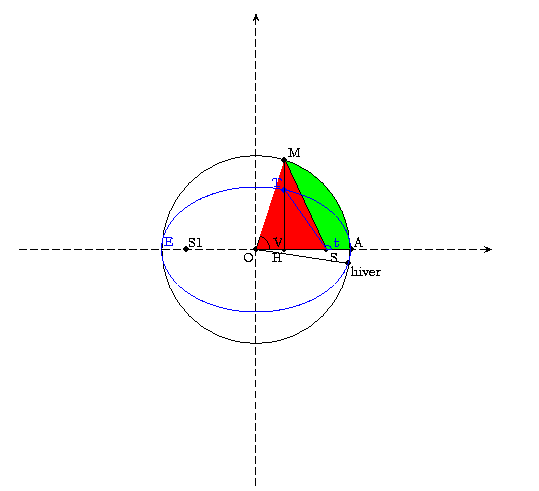
\includegraphics[width=\textwidth]{ellipse}
\caption{Ellipse et \'equation du temps}
\end{figure}
La trajectoire elliptique $E$ de la Terre autour du Soleil est
représentée sur la figure \ref{fig:ell}
en bleu, l'excentricité de l'orbite a été énormément exagérée, il
s'agit d'une ellipse de foyers $S$ (le Soleil) et $S'$. Le point $A$ désigne
le p\'erihélie de l'orbite (passage de la Terre au plus proche du Soleil), 
qui a lieu
vers le 4 janvier. En noir, on a dessiné le grand cercle de l'ellipse
(l'ellipse s'obtient par contraction du grand cercle de rapport $\sqrt{1-e^2}$
où $e$ est l'excentricité de l'orbite).
L'aire décrite par le rayon Soleil-Terre ($ST$)
est proportionnelle au temps (loi des aires qui découle de la conservation
du moment cinétique), 
il en est donc de même de l'aire (en vert) du
décrite par le rayon $SM$. Si on ajoute à cette aire verte l'aire en 
rouge du triangle $OSM$, on obtient l'aire de l'arc de cercle $OAM$.
Donc
\[ \frac{1}{2} V \times OA^2 - \frac{1}{2} OS \times HM \]
est proportionnel au temps écoulé depuis le passage au p\'erihélie.
Comme $HM=OM \sin(V)$ et $OS= e \times OA$, on en déduit que 
\begin{equation} \label{eq:tempsV}
 V - e \sin(V) = C t = 2\pi \frac{t}{T}
\end{equation}
où la constante $C$ s'obtient en faisant varier $V$ de 0 à $2\pi$
ce qui correspond à la durée $T$ d'une révolution de la Terre 
autour du Soleil (1 an).

La relation entre $\theta$ (not\'e $t$ sur la figure)
et $V$ s'obtient par exemple en calculant 
l'abscisse de $M$ 
\begin{eqnarray*} 
x &= &a \cos(V) \\
 &= & ea + \rho \cos(\theta) \\
 &= & ea + a\frac{1-e^2}{1+e\cos(\theta)} \cos(\theta)
\end{eqnarray*}
Les angles $V$ et $\theta$ sont de même signe et
\begin{equation} \label{eq:Vt}
 \cos(V) = \frac{\cos(\theta)+e}{1+e\cos(\theta)}
\end{equation}
et réciproquement~:
\begin{equation} \label{eq:tV}
 \cos(\theta)=\frac{\cos(V)-e}{1-e \cos(V)} 
\end{equation}

{\bf Durée des saisons~}:\\
Il suffit de connaitre l'angle $\theta$ lors du solstice d'hiver et
de lui ajouter $k\pi/2$ pour $k=1,2,3$ pour connaitre l'angle $\theta$
au printemps, en été et à l'automne, on en déduit $V$ par (\ref{eq:Vt}) 
puis le temps écoulé depuis le p\'erihélie avec (\ref{eq:tempsV}).

{\bf Calcul de $\theta$ en fonction du temps écoulé depuis le passage
au p\'erihélie}~:\\
Il faut calculer $V$ par des méthodes numériques (point fixe ou 
méthode de Newton) en appliquant (\ref{eq:tempsV}), on en déduit
$\theta$ avec (\ref{eq:tV}).
En résumé, on a le~:
\begin{thm}
Soit $\theta$ l'angle entre le demi grand axe de l'ellipse et 
la direction Soleil-Terre, $t\in [-T/2,T/2]$ le temps écoulé depuis le passage
au périhélie ($t=0$ lorsque $\theta=0$, $T=1$ an). Soit $V\in [-\pi,\pi]$ 
la solution de 
\[  V - e \sin(V) = 2\pi \frac{t}{T} \]
où $e$ est l'excentricité de l'ellipse.
Alors $\theta$ est donné par
\[  \cos(\theta)=\frac{\cos(V)-e}{1-e \cos(V)}  \]
\end{thm}

\subsection{Les variations des paramètres orbitaux}
La Terre n'est pas une sphère idéale, elle a un renflement au niveau
de l'équateur, due à rotation de la Terre sur elle-même (la force
centrifuge y est plus importante). Ce renflement est dans un plan
qui fait un angle avec le plan de l'écliptique, le Soleil exerce
donc un couple sur ce renflement. Ce phénomène est à l'origine
de la précession des équinoxes, le passage au p\'erihélie de la Terre
se décale dans le temps.
De plus, la Terre n'est pas seulement soumise à l'influence du Soleil,
mais aussi des autres planètes, en particulier Jupiter. Cela
modifie sur de très longues périodes tous les paramètres
de l'orbite terrestre, en particulier l'excentricité, la précession
des équinoxes, mais aussi l'obliquité (inclinaison de l'axe de
rotation terrestre par rapport à la perpendiculaire au plan de
l'écliptique).
Le calcul de ces variations est bien au-delà des prétentions de ce texte,
le lecteur intéressé pourra se référer par exemple aux publications
de Laskar (chercher ce mot-clef ou des mots comme orbite,
perturbation, symplectique, hamiltonien, ...). On se bornera ici
\`a indiquer que le demi-grand axe ne varie pas, ce qui donne
une relation entre les variations de la constante des aires et 
de l'excentricit\'e 
\[ L \mbox{ est proportionnel \`a } \sqrt{1-e^2}\]

Les variations des paramètre orbitaux
modifient à long terme l'ensolleillement de la Terre (la valeur
de l'énergie reçue en un lieu sur une surface horizontale $s.v/\rho^2$
dépend de la latitude, de la position de la Terre sur son orbite
mais aussi de l'excentricité de l'orbite, de l'obliquité
et de la date du p\'erihélie par rapport aux saisons) et
sa répartition sur le globe par latitude, il est naturel de supposer
qu'elles influent sur le climat de la Terre.
Par exemple, l'\'energie moyenne recue par la Terre au cours d'une
p\'eriode $T$ de une ann\'ee est donn\'ee par
\[ \frac{1}{T}\int_0^{T} \frac{dt}{\rho^2} = 
\frac{1}{T}\int_0^{2\pi} \frac{d\theta}{L} = \frac{2 \pi}{T L}  \]
est proportionnelle \`a $\frac{1}{(T L)}$ donc \`a $(1-e^2)^{-1/2}$ (car
$T$ est aussi constant d'apr\`es la 3\`eme loi de K\'epler).
Au premier ordre, la variation de $e$ entraine donc une variation de 
l'ensolleillement global de
\[ \frac{1}{2} e^2\]
Pour la Terre, cela repr\'esente au plus 2.5 pour mille (la p\'eriode
la plus favorable aux glaciations \'etant celle o\`u l'orbite est
circulaire), soit, sans r\'etroactions, une variation globale
de 0.2 degr\'es Kelvin.


\section{La moyenne arithm\'etico-g\'eom\'etrique.}
\label{sec:agm}
\index{moyenne arithm\'etico-g\'eom\'etrique}
La moyenne arithm\'etico-g\'eom\'etrique est un processus it\'eratif
qui converge tr\`es rapidement et est tr\`es utile pour calculer
les fonctions transcendantes r\'eciproques en multi-pr\'ecision. 
On peut alors trouver les fonctions transcendantes directes
par application de la m\'ethode de Newton.

\subsection{D\'efinition et convergence}
Soient $a$ et $b$ deux r\'eels positifs,
on d\'efinit les 2 suites 
\begin{equation} \label{eq:agm}
 u_0=a, v_0=b, \quad u_{n+1}=\frac{u_n+v_n}{2}, v_{n+1}=\sqrt{u_nv_n} 
\end{equation}
On va montrer que ces 2 suites sont adjacentes et convergent donc vers
une limite commune not\'ee $M(a,b)$ et il se trouve que la convergence
est tr\`es rapide, en raison de l'identit\'e~:
\begin{equation} \label{eq:agm1}
u_{n+1}-v_{n+1}=\frac{1}{2}(\sqrt{u_n}-\sqrt{v_n})^2
=\frac{1}{2(\sqrt{u_n}+\sqrt{v_n})^2}(u_n-v_n)^2
\end{equation}
la convergence est quadratique.

On suppose dans la suite que $a\geq b$ sans changer la généralité puisque échanger $a$ et $b$
ne change pas la valeur de $u_n$ et $v_n$ pour $n>0$. On a alors $u_n \geq v_n$ 
(d'après (\ref{eq:agm1}) pour $n>0$) et $u_{n+1} \leq u_n$ car
\[ u_{n+1}-u_n=\frac{1}{2}(v_n-u_{n}) \leq 0\]
et $v_{n+1}=\sqrt{u_nv_n} \geq \sqrt{v_nv_n}=v_n$. Donc $(u_n)$ est décroissante 
minorée (par $v_0$), $(v_n)$ est croissante majorée (par $u_0$), ces 2 suites sont 
convergentes et comme $u_{n+1}=\frac{u_n+v_n}{2}$, elles convergent vers la même limite 
$l$ qui d\'epend de $a$ et $b$ et que l'on note $M(a,b)$.
On remarque aussi que $M(a,b)=bM(a/b,1)=aM(1,b/a)$. 

Précisons maintenant la vitesse de convergence lorsque $a \geq b>0$. 
On va commencer par estimer le nombre
d'itérations nécessaires pour que $u_n$ et $v_n$ soient du même ordre de grandeur.
Pour cela, on utilise la majoration
\[ \ln(u_{n+1})-\ln(v_{n+1}) \leq \ln(u_{n})-\ln(v_{n+1}) = \frac{1}{2}
(\ln(u_{n})-\ln(v_{n})) \]
donc
\[ \ln \frac{u_n}{v_n} = \ln(u_n)-\ln(v_n) \leq 
\frac{1}{2^n} (\ln(a)-\ln(b)) = \frac{1}{2^n} \ln \frac{a}{b} \]
Donc si $n \geq \frac{\ln( \ln(a/b)/m)}{\ln(2)}$ alors
$\ln \frac{u_n}{v_n} \leq m$ (par exemple, on peut prendre $m=0.1$ pour 
avoir $u_n/v_n \in [1,e^{0.1}])$. Le nombre minimum d'itérations $n_0$ est proportionnel
au log du log du rapport $a/b$.
Ensuite on est ramené à étudier la convergence de la suite arithmético-géométrique
de premiers termes $a=u_{n_0}$ et $b=v_{n_0}$ et même en tenant compte
de $M(a,b)=aM(1,b/a)$ à $a=1$ et $b=v_n/u_n$ donc $0\leq a-b \leq 1-e^{-0.1}$.
Alors l'équation (\ref{eq:agm1}) entraine 
\[ u_{n+1}-v_{n+1} \leq \frac{1}{8}(u_n-v_n)^2 \]
puis (par récurrence)
\[ 0 \leq u_n-v_n \leq \frac{1}{8^{2^n-1}}(a-b)^{2^n} \]
Donc comme $M(a,b)$ est compris entre $v_n$ et $u_n$, l'erreur relative sur la limite
commune est inférieure à une précision donnée $\epsilon$
au bout d'un nombre d'itérations proportionnel au $\ln(\ln(1/\epsilon))$.

Typiquement dans la suite, on souhaitera calculer $M(1,b)$ avec $b$ de l'ordre
de $2^{-n}$ en déterminant $n$ chiffres significatifs,
il faudra alors $O(\ln(n))$ itérations pour se ramener à $M(1,b)$ avec $b\in [e^{-0.1},1]$ 
puis $O(\ln(n))$ itérations pour avoir la limite avec $n$ chiffres significatifs.

{\bf Le cas complexe}\\
On suppose maintenant que $a, b \in \C$ avec $\Re(a)>0, \Re(b)>0$. On va voir que
la suite arithmético-géométrique converge encore. \\
{\bf \'Etude de l'argument}\\
On voit aisément (par récurrence)
que $\Re(u_n)>0$ ; de plus $\Re(v_n) > 0$ car par définition de la racine carrée
$\Re(v_n)\geq 0$ et est de plus non nul car le produit de deux complexes d'arguments dans 
$]-\pi/2,\pi/2[$ ne peut pas être un réel négatif.
On en déduit que
$\arg(u_{n+1})=\arg(u_n+v_n)$ se trouve dans l'intervalle de bornes
$\arg(u_n)$ et $\arg(v_n)$ et que $\arg(v_{n+1})=\frac{1}{2}(\arg(u_n)+\arg(v_n))$
donc
\[ | \arg(u_{n+1}-\arg(v_{n+1}) | \leq \frac{1}{2}|\arg(u_n)-\arg(v_n)| \]
Après $n$ itérations, on a 
\[ |\arg(u_n)-\arg(v_n)| \leq \frac{\pi}{2^n} \]
Après quelques itérations, $u_n$ et $v_n$ seront donc presque alignés. 
Faisons 4 itérations.
On peut factoriser par exemple $v_n$ et on
est ramené à l'étude de la suite de termes initiaux $a=u_n/v_n$ d'argument 
$\arg(u_n)-\arg(v_n)$ petit 
(inférieur en valeur absolue à $\pi/16$) et $b=1$. On suppose donc dans la suite que
\[ |\arg(\frac{u_n}{v_n})| \leq \frac{\pi/16}{2^n} \]
{\bf \'Etude du module}\\
On a~:
\[ \frac{u_{n+1}}{v_{n+1}}= \frac{1}{2}\left(\sqrt{\frac{u_{n}}{v_{n}}}+\frac{1}{\sqrt{\frac{u_{n}}{v_{n}}}}\right)  \]
Posons $ \frac{u_{n}}{v_{n}}=\rho_n e^{i\theta_n}$, on a~:
\begin{eqnarray*} 
|\frac{u_{n+1}}{v_{n+1}}| &= & \frac{1}{2}\left|\sqrt{\rho_n} e^{i\theta_n/2}
+ \frac{1}{\sqrt{\rho_n}} e^{-i\theta_n/2} \right| \\
&=& \frac{1}{2} \left| (\sqrt{\rho_n}+ \frac{1}{\sqrt{\rho_n}})\cos\frac{\theta_n}{2}
+ i (\sqrt{\rho_n}- \frac{1}{\sqrt{\rho_n}})\sin\frac{\theta_n}{2} \right| \\
&=& \frac{1}{2} \sqrt{ (\sqrt{\rho_n}+ \frac{1}{\sqrt{\rho_n}})^2\cos^2\frac{\theta_n}{2}
+ (\sqrt{\rho_n}- \frac{1}{\sqrt{\rho_n}})^2\sin^2\frac{\theta_n}{2} } \\
&=& \frac{1}{2} \sqrt{ \rho_n+ \frac{1}{\rho_n} +2\cos \theta_n }
\end{eqnarray*}
Si $\rho$ désigne le max de $\rho_n$ et $1/\rho_n$, on a alors la majoration
\[ |\frac{u_{n+1}}{v_{n+1}}| \leq \frac{1}{2} \sqrt{ \rho + \rho + 2 \rho } 
= \sqrt{\rho} \]
donc en prenant les logarithmes
\begin{equation} \label{eq:lnrhon}
\ln \rho_{n+1} \leq \frac{1}{2}  \ln \rho=\frac{1}{2}  |\ln \rho_n| 
\end{equation}
On rappelle qu'on a la majoration 
\[ |\arg(\frac{u_n}{v_n})| = |\theta_n| \leq \frac{\pi/16}{2^n} \leq \frac{1}{2^{n+1}} \]
qui va nous donner la minoration de $\rho_{n+1}$ 
\begin{eqnarray*}
\rho_{n+1}=|\frac{u_{n+1}}{v_{n+1}}| & = & \frac{1}{2}
\sqrt{ \rho_n+ \frac{1}{\rho_n} +2 - 2 (1-\cos \theta_n) } \\
& = &  \frac{1}{2} \sqrt{ \rho_n+ \frac{1}{\rho_n} +2 - 4 \sin^2 (\frac{\theta_n}{2}) } \\
& \geq &  \frac{1}{2} \sqrt{ \rho_n+ \frac{1}{\rho_n} +2 - \theta_n^2} \\
& \geq &  \frac{1}{2} \sqrt{ \rho_n+ \frac{1}{\rho_n} +2} \times 
\sqrt{1 - \frac{\theta_n^2}{\rho_n+ \frac{1}{\rho_n} +2}} \\
& \geq &  \frac{1}{2} \sqrt{ \frac{1}{\rho} + \frac{1}{\rho} +2\frac{1}{\rho}} \times 
\sqrt{1 - \frac{\theta_n^2}{4}} \\
& \geq & \frac{1}{\sqrt{\rho}} \sqrt{1 - \frac{\theta_n^2}{4}} \\
& \geq & \frac{1}{\sqrt{\rho}} \sqrt{1 - \frac{1} {4 \times 2^{2n+2}}}
\end{eqnarray*}
en prenant les log et en minorant $\ln(1-x)$ par $-2x$
\[ \ln \rho_{n+1} \geq \frac{1}{2} (-|\ln \rho_n|+\ln(1 -\frac{1} {4 \times 2^{2n+2}} ))
\geq -\frac{1}{2} (|\ln \rho_n|+\frac{1} {2^{2n+3}} )  \]
Finalement avec (\ref{eq:lnrhon})
\[ |\ln \rho_{n+1}|
\leq \frac{1}{2} (|\ln \rho_n|+\frac{1}{2^{2n+3}} ) \]
On en déduit
\[ |\ln \rho_n| \leq \frac{1}{2^n} \ln \rho_0 + \frac{1}{2^{n+3}} + ... +
\frac{1}{2^{2n+1}} +  \frac{1}{2^{2n+2}}
= \frac{1}{2^n} \ln \rho_0 + \frac{1}{2^{n+2}} \]
La convergence du $\ln(u_n/v_n)$ vers 0 est donc géométrique, donc $u_n$ et $v_n$ convergent
quadratiquement.

\subsection{Lien avec les int\'egrales elliptiques}\index{elliptique, int\'egrale}
Le calcul de la limite commune des suites $u_n$ et $v_n$ en fonction
de $a$ et $b$ n'est pas trivial
au premier abord. Il est reli\'e aux int\'egrales elliptiques, plus
pr\'ecis\'ement on peut construire une int\'egrale d\'ependant
de deux param\`etres $a$ et $b$ et qui est invariante par
la transformation $u_n,v_n \rightarrow u_{n+1},v_{n+1}$ (\ref{eq:agm})
\[ I(a,b)=\int_{-\infty}^{+\infty}  \frac{dt} {\sqrt{(a^2+t^2)(b^2+t^2)}}
\]
On a en effet
\[ I(\frac{a+b}{2},\sqrt{ab})
= \int_{-\infty}^{+\infty}  \frac{du}{\sqrt{((\frac{a+b}{2})^2+u^2)(ab+u^2)}} \]
On pose alors 
\[ u=\frac{1}{2} (t-\frac{ab}{t}), \quad t>0 \]
o\`u $t \rightarrow u$ est une bijection croissante de $t\in]0,+\infty[$ vers 
$u \in ]-\infty,+\infty[$, donc
\begin{eqnarray*}
I(\frac{a+b}{2},\sqrt{ab})
&=& \int_{0}^{+\infty}  \frac{dt/2(1+ab/t^2)}{\sqrt{((\frac{a+b}{2})^2+1/4(t-ab/t)^2)(ab+1/4(t-ab/t)^2)}}\\
&=& 2 \int_{0}^{+\infty} \frac{dt}{\sqrt{(a^2+t^2)(b^2+t^2)}}
= I(a,b)
\end{eqnarray*}
On note au passage que $I$ est définie si $a,b \in \C$ vérifient $\Re(a)>0, \Re(b)>0$,
on peut montrer que la relation ci-dessus s'étend (par holomorphie).

Lorsque $a=b=l$ (par exemple lorsqu'on est \`a la limite), 
le calcul de $I(l,l)$ est explicite
\[ I(l,l)=\int_{-\infty}^{+\infty}  \frac{dt}{(l^2+t^2)} = \frac{\pi}{l}\]
donc
\[ I(a,b)=I(M(a,b),M(a,b))=\frac{\pi}{M(a,b)}\]
On peut transformer $I(a,b)$ en posant $t=bu$
\[ I(a,b)=2\int_{0}^{+\infty}  \frac{du}{\sqrt{(a^2+b^2u^2)(1+u^2)}}
= \frac{2}{a} \int_{0}^{+\infty}  \frac{du}{\sqrt{(1+(b/a)^2u^2)(1+u^2)}} \]
Puis en posant $u=\tan(x)$ ($du=(1+u^2) dx$)
\[ I(a,b)=\frac{2}{a} \int_0^{\frac{\pi}{2}} 
\sqrt{\frac{1+\tan(x)^2}{1+(b/a)^2\tan(x)^2}} \ dx \]
et enfin en posant $\tan^2(x)=\frac{\sin(x)^2}{1-\sin(x)^2}$
\[ I(a,b)= \frac{2}{a} \int_0^{\frac{\pi}{2}}  
\sqrt{ \frac{1}{1-(1-\frac{b^2}{a^2})\sin(x)^2} } \ dx\]
Si on d\'efinit pour $m<1$
\[ K(m)=\int_0^{\frac{\pi}{2}} \frac{dx}{\sqrt{1-m \sin(x)^2}} \]
alors on peut calculer $K$ en fonction de $I$, en posant
$m=1-b^2/a^2$ soit $b^2/a^2=1-m$
\[ K(m)=\frac{a}{2} I(a,a\sqrt{1-m})=\frac{a}{2}\frac{\pi}{M(a,a\sqrt{1-m})}
=\frac{\pi}{2M(1,\sqrt{1-m})} 
\]
d'o\`u l'on d\'eduit la valeur de l'int\'egrale elliptique en fonction
de la moyenne arithm\'etico-g\'eom\'etrique~:
\begin{equation} \label{eq:K}
K(m)=\int_0^{\frac{\pi}{2}} \frac{dx}{\sqrt{1-m \sin(x)^2}}= 
\frac{\pi}{2M(1,\sqrt{1-m})} 
\end{equation}
Dans l'autre sens, pour $x$ et $y$ positifs
\[ K( (\frac{x-y}{x+y})^2 )=  \frac{\pi}{2M(1,\sqrt{1-(\frac{x-y}{x+y})^2})}
=  \frac{\pi}{2M(1,\frac{2}{x+y}\sqrt{xy})}
= \frac{\pi}{2 \frac{2}{x+y} M(\frac{x+y}{2},\sqrt{xy}) }
= \frac{\pi}{4} \frac{x+y}{M(x,y)}
\]
et finalement
\[ M(x,y)=\frac{\pi}{4} \frac{x+y}{ K\left( (\frac{x-y}{x+y}\right)^2 )}\]

\subsection{Application~: calcul efficace du logarithme.}\index{logarithme}
On peut utiliser la moyenne arithm\'etico-g\'eom\'etrique pour
calculer le logarithme efficacement, pour cela on cherche le d\'eveloppement
asymptotique de $K(m)$ lorsque $m$ tend vers 1. Plus pr\'ecis\'ement,
on va poser $1-m=k^2$ avec $k \in ]0,1]$, donc
\[ K(m)= \int_0^{\frac{\pi}{2}} \frac{dx}{\sqrt{1-(1-k^2) \sin(x)^2}}
=\int_0^{\frac{\pi}{2}} \frac{dy}{\sqrt{1-(1-k^2) \cos(y)^2}}
\]
en posant $y=\pi/2-x$, et
\[ K(m)=\int_0^{\frac{\pi}{2}} \frac{dy}{\sqrt{\sin(y)^2+k^2 \cos(y)^2}}\]
la singularit\'e de l'int\'egrale pour $k$ proche
de 0 apparait lorsque $y$ est proche de 0.
Si on effectue un d\'eveloppement de Taylor en $y=0$, on trouve
\[ \sin(y)^2+k^2 \cos(y)^2 = k^2 + (1-k^2) y^2 + O(y^4)\]
Il est donc naturel de comparer $K(m)$ \`a l'int\'egrale
\[ J=\int_0^{\frac{\pi}{2}} \frac{dy}{\sqrt{k^2 + (1-k^2) y^2}} \]
qui se calcule en faisant par exemple le changement de variables
\[ y=\frac{k}{\sqrt{1-k^2}} \sinh(t)\]
ou directement avec Xcas, 
\begin{center}
\verb|supposons(k>0 && k<1);|\\
\verb|J:=int(1/sqrt(k^2+(1-k^2)*y^2),y,0,pi/2)|
\end{center}
qui donne apr\`es r\'e\'ecriture~:
\begin{equation} \label{eq:J}
 J= \frac{1}{\sqrt{1-k^{2}}}
\left( \ln\left(\frac{\pi}{k}\right) +
\ln\left( \frac{1}{2} \left(\sqrt{ 1-k^{2} +4 \frac{k^{2}}{\pi^2}} 
+\sqrt{1-k^{2}} \right) \right) \right)
\end{equation}
et on peut calculer le d\'eveloppement asymptotique de $J$ en 0
\begin{center}
\verb|series(J,k=0,5,1)|
\end{center}
qui renvoie~:
\[ J =\ln\left(\frac{\pi}{k}\right) +O( \left(\frac{-1}{\ln(k)}\right)^5)\]
on peut alors pr\'eciser ce d\'eveloppement par
\begin{center}
\verb|series(J+ln(k)-ln(pi),k=0,5,1)|
\end{center}
qui renvoie (apr\`es simplifications et où la notation $\tilde{O}$ peut contenir des logarithmes)
\[ \left(\frac{1}{\pi^2} + \frac{\ln(\pi)-\ln(k)-1}{2}\right) k^{2} + 
\tilde{O}(k^4)\]
donc
\begin{equation}
J=-\ln(k)+\ln(\pi)+\left(\frac{1}{\pi^2} + 
\frac{\ln(\pi)-\ln(k)-1}{2}\right) k^{2} + \tilde{O}(k^4)
\end{equation}
Examinons maintenant $K-J$, il n'a plus de singularit\'e en $y=0$, et il admet une limite
lorsque $k \rightarrow 0$, obtenue en remplacant $k$ par 0
\[ (K-J)_{|k=0} = \int_0^{\frac{\pi}{2}} \left(\frac{1}{\sin(y)}-\frac{1}{y}\right)
\ dy = \left[\ln\left(\tan\left(\frac{y}{2}\right)\right) - \ln(y) \right]_0^{\frac{\pi}{2}} =
\ln(\frac{4}{\pi})\]
D'o\`u pour $K$
\[ K_{k \rightarrow 0} = \ln\left(\frac{4}{k}\right) + O( \left(\frac{-1}{\ln(k)}\right)^5)\]
Pour pr\'eciser la partie du d\'eveloppement de $K$ en puissances de $k$, nous allons
majorer $K-J-\ln(4/\pi)$, puis $J-\ln(\pi/k)$.
Posons
\[ A=\sin(y)^2+k^2 \cos(y)^2, \quad B=y^2+(1-y^2)k^2\]
{\bf Majoration de $K-J-\ln(4/\pi)$}\\
L'int\'egrand de la diff\'erence $K-J-\ln(\frac{4}{\pi})$ est
\begin{eqnarray}  
\frac{1}{\sqrt{A}} - \frac{1}{\sqrt{B}} - 
\left( \frac{1}{\sin(y)}-\frac{1}{y} \right)
&= &
\frac{\sqrt{B}-\sqrt{A}}{\sqrt{A} \sqrt{B}} -
\frac{y-\sin(y)}{y\sin(y)} 
 \\
&= &
\frac{B-A}{\sqrt{A} \sqrt{B} (\sqrt{A}+\sqrt{B})} -
\frac{y-\sin(y)}{y\sin(y)} \label{eq:maj0}
 \\
&=& \frac{(y^2-\sin(y)^2)(1-k^2)}{\sqrt{A} \sqrt{B} (\sqrt{A}+\sqrt{B})}
- \frac{y-\sin(y)}{y\sin(y)} \label{eq:maj1}
\end{eqnarray}
Soit
\begin{equation} \label{eq:maj2}
 K-J-\ln(\frac{4}{\pi})= \int_0^{\frac{\pi}{2}} 
\frac{(y-\sin(y))[(1-k^2)y \sin(y)(y+\sin(y))-\sqrt{AB}(\sqrt{A}+\sqrt{B})]}
{\sqrt{A} \sqrt{B} (\sqrt{A}+\sqrt{B})y\sin(y)}
\end{equation}
On décompose l'intégrale en 2 parties $[0,k]$ et $[k,\pi/2]$.
Sur $[0,k]$ on utilise (\ref{eq:maj0}), on majore chaque terme séparément
et on minore $A$ et $B$ par
\[ A=k^2+(1-k^2)\sin(y)^2 \geq k^2, \quad B=k^2+(1-k^2)y^2 \geq k^2\]
Donc
\begin{eqnarray*} 
| \int_0^{k} | &\leq &\int_0^k \frac{|B-A|}{2k^3} \ dy + \int_0^k ( \frac{1}{\sin(y)}-\frac{1}{y} ) 
\ dy \\
&\leq& \int_0^k \frac{y^2-\sin(y)^2}{2k^3} \ dy + \ln (\tan(\frac{k}{2})) -\ln(\frac{k}{2}) \\
&\leq & \frac{\frac{1}{3} k^{3}+\frac{-1}{2} k+\frac{1}{4} \sin(2 k)}{2 k^{3}} 
+ \ln (\sin(\frac{k}{2})) -\ln(\frac{k}{2}) - \ln (\cos(\frac{k}{2}))
\\
&\leq & \frac{\frac{1}{3} k^{3}+\frac{-1}{2} k+\frac{1}{4} (2k-\frac{8k^3}{6}+\frac{32k^5}{5!}}{2 k^{3}} - \ln (\cos(\frac{k}{2})) \\
&\leq & \frac{k^2}{30}-  \ln (1- \frac{1}{2!}\left(\frac{k}{2}\right)^2) \\
&\leq &  \frac{k^2}{30} +\frac{k^2}{4}
\end{eqnarray*}
Sur $[k,\pi/2]$, on utilise (\ref{eq:maj2})
et on minore $A$ et $B$ par
\[ A=\sin(y)^2+k^2 \cos(y)^2 \geq \sin(y)^2, \quad B=y^2+(1-y^2)k^2 \geq y^2\]
on obtient
\[ 
| \int_k^{\frac{\pi}{2}} | \leq  \int_k^{\frac{\pi}{2}}
\frac{(y-\sin(y))|C|}
{y \sin(y) (y+\sin(y))} , 
\]
où~:
\begin{eqnarray*}
C&=&(1-k^2)y \sin(y)(y+\sin(y))-A\sqrt{B}+B\sqrt{A} \\
&=& -A(\sqrt{B}-y)-B(\sqrt{A}-\sin(y))
-Ay-B\sin(y) + (1-k^2)y \sin(y)(y+\sin(y)) \\
&=& -A(\sqrt{B}-y)-B(\sqrt{A}-\sin(y)) - k^2(y+\sin(y))
\end{eqnarray*}
Donc
\begin{eqnarray*}
 |C| &\leq& A(\sqrt{B}-y)+B(\sqrt{A}-\sin(y)) + k^2(y+\sin(y)) \\
&\leq& A \frac{B-y^2}{\sqrt{B}+y}
+ B \frac{A-\sin(y)^2}{\sqrt{A}+\sin(y)} + k^2(y+\sin(y)) \\
&\leq & A \frac{k^2}{2y} + B \frac{k^2}{2\sin(y)} + k^2(y+\sin(y))
\end{eqnarray*}
et
\[ 
| \int_k^{\frac{\pi}{2}} | \leq 
\int_k^{\frac{\pi}{2} }
\frac{(y-\sin(y))k^2(\frac{A}{2y} + \frac{B}{2\sin(y)} + (y+\sin(y))) }
{y \sin(y) (y+\sin(y))}
\]
On peut majorer $y-\sin(y) \leq y^3/6$, donc
\[ 
| \int_k^{\frac{\pi}{2}} | \leq 
\frac{k^2}{6} \int_k^{\frac{\pi}{2}}
 \frac{Ay}{2\sin(y) (\sin(y)+y)} + \frac{By^2}{\sin(y)^2(\sin(y)+y)} + \frac{y^2}{\sin(y)}
\]
On majore enfin $A$ et $B$ par 1, 
\[ | \int_k^{\frac{\pi}{2}} |
\leq \frac{k^2}{6} \int_k^{\frac{\pi}{2}}
\frac{y}{2\sin(y)^2} + \frac{y^2}{\sin(y)}
\]
Le premier morceau se calcule par intégration par parties
\begin{eqnarray*}
\frac{k^2}{6} \int_k^{\frac{\pi}{2}}
\frac{y}{2\sin(y)^2}
&=&
\frac{k^2}{6} \left( [-\frac{y}{\tan(y)}]_k^{\pi/2} 
+ \int_k^{\frac{\pi}{2}} \frac{1}{\tan(y)}
\right) \\
&=& \frac{k^2}{6} \left(\frac{k}{\tan(k)}+ [\ln(\sin(y))]_k^{\frac{\pi}{2}} \right)\\
&=& \frac{k^2}{6} \left(\frac{k}{\tan(k)}-\ln(\sin(k)) \right)\\
&\leq &  \frac{k^2}{6}(1-\ln(k))
\end{eqnarray*}
Le deuxième morceau se majore en minorant $\sin(y)\geq (2y)/\pi$
\[ 
\frac{k^2}{6} \int_k^{\frac{\pi}{2}} \frac{y^2}{\sin(y)}
\leq \frac{k^2}{6} \int_0^{\frac{\pi}{2}} \frac{\pi}{2} y
= \frac{k^2\pi^3}{96} 
\]
Finalement
\[ |K-J-\ln(\frac{4}{\pi})| 
\leq k^2 \left( -\frac{1}{6} \ln(k) + \frac{\pi^3}{96} + \frac{1}{6} + \frac{1}{30}+ 
\frac{1}{4} \right)
\]
où $J$ est donné en (\ref{eq:J}).

{\bf Majoration de $J-ln(\pi/k)$}\\
On a
\[ |J - \ln\left(\frac{\pi}{k}\right)|
= \left| (\frac{1}{\sqrt{1-k^2}}-1) \ln\left(\frac{\pi}{k}\right)
+ \frac{1}{\sqrt{1-k^2}}
\ln\left( \frac{1}{2} \left(\sqrt{ 1-k^{2} +4 \frac{k^{2}}{\pi^2}} 
+\sqrt{1-k^{2}} \right) \right) \right| \]
et on va majorer la valeur absolue de chaque terme de la somme.
Pour $k\leq 1/2$, on a
\[ \frac{1}{\sqrt{1-k^2}}-1=\frac{k^2}{\sqrt{1-k^2}+1-k^2} \leq \frac{k^2}{3/4+\sqrt{3}/2} \]
Pour le second terme, on majore le facteur $\frac{1}{\sqrt{1-k^2}}$ par $\frac{2}{\sqrt{3}}$,
l'argument du logarithme est inférieur à 1 et supérieur à
\[ 
\frac{1}{2}(1 - \frac{k^2}{2} +1- \frac{k^2(1-\frac{4}{\pi^2})}{2})
= 1 - k^2 ( 1-\frac{1}{\pi^2}) > 1-k^2
\]
donc le logarithme en valeur absolue est inférieur à
\[ 2 k^2 \]
donc, pour $k\leq 1/2$,
\[ |J-\ln\left(\frac{\pi}{k}\right)| \leq 
\frac{k^2}{3/4+\sqrt{3}/2} \ln\left(\frac{\pi}{k}\right)
+ k^2 \frac{4}{\sqrt{3}} 
\]
Finalement, pour $k<1/2$
\begin{equation} \label{eq:ln_agm0}
 |K-\ln\left(\frac{4}{k}\right) | 
\leq k^2 \left( \frac{\ln \pi}{3/4+\sqrt{3}/2}  + \frac{4}{\sqrt{3} }
+ \frac{\pi^3}{96} + \frac{9}{20}
- (\frac{1}{3/4+\sqrt{3}/2}+\frac{1}{6}) \ln(k) \right) 
\end{equation}
que l'on peut réécrire
\begin{equation} \label{eq:ln_agm}
|\frac{\pi}{2M(1,k)}-\ln\left(\frac{4}{k}\right) |
\leq  k^2(3.8-0.8\ln(k))
\end{equation}
La formule (\ref{eq:ln_agm}) 
permet de calculer le logarithme d'un r\'eel positif
avec (presque) $n$ bits 
lorsque $k \leq 2^{-n/2}$ (ce \`a quoi on peut toujours se ramener
en calculant le logarithme d'une puissance $2^m$-i\`eme de $x$ ou
le logarithme de $2^{m}x$, en calculant au pr\'ealable $\ln(2)$).
Par exemple, prenons $k=2^{-27}$, on trouve (en 8 itérations)
$M(1,2^-{27})=M_1=0.0781441403763$. 
On a, avec une erreur inférieure à $19 \times 2^{-54}=1.1\times 10^{-15}$
\[ 
M(1,2^-{27})=M_1=\frac{\pi}{2\ln(2^{29})}=\frac{\pi}{58\ln(2)},
\] 
On peut donc d\'eduire une valeur approch\'ee de $\pi $ si on connait
la valeur approchée de $\ln(2)$ et réciproquement.
Si on veut calculer les deux simultan\'ement, comme les relations entre $\ln$
et $\pi$ seront des \'equations homog\`enes, on est oblig\'e
d'introduire une autre relation. Par exemple pour calculer une
valeur approch\'ee de $\pi$ on calcule la diff\'erence
$\ln(2^{29}+1)-\ln(2^{29})$ dont on connait le d\'eveloppement au premier
ordre, et on applique la formule de la moyenne arithm\'etico-g\'eom\'etrique.
Il faut faire attention \`a la perte de pr\'ecision lorsqu'on fait
la diff\'erence des deux logarithmes qui sont tr\`es proches, ainsi
on va perdre une trentaine de bits (de m\^eme pour les moyennes).
On peut aussi calculer $\pi$ directement avec $M(1,\sqrt(2))$ en
utilisant des propri\'et\'es des int\'egrales elliptiques\index{pi,
  calcul de}
\begin{verbatim}
f(n):={
  local x,y,z,p;
  x:=evalf(1/sqrt(2),2^n);
  y:=(1+x)/2/sqrt(x);
  z:=1/sqrt(x);
  p:=evalf(2+sqrt(2),2^n);
  for k from 1 to n do
    p,y,z:=p*(1+y)/(1+z),(1+y)/sqrt(y)/2,(1+y*z)/(1+z)/sqrt(y);
  od;
  retourne p;
}:;
\end{verbatim}

L'int\'er\^et de cet algorithme apparait lorsqu'on veut calculer
le logarithme avec beaucoup de pr\'ecision, en raison de la
convergence quadratique de la moyenne arithm\'etico-g\'eom\'etrique
(qui est nettement meilleure que la convergence lin\'eaire
pour les d\'eveloppements en s\'erie, ou logarithmiquement
meilleure pour l'exponentielle), par contre elle n'est pas
performante si on ne veut qu'une dizaine de chiffres significatifs. 
On peut alors calculer les autres
fonctions transcendantes usuelles, telle l'exponentielle,
\`a partir du logarithme, ou les fonctions trigonom\'etriques
inverses (en utilisant des complexes) et directes.

On trouvera dans Brent-Zimmermann quelques consid\'erations permettant
d'am\'eliorer les constantes dans les temps de calcul par rapport
\`a cette m\'ethode (cela n\'ecessite d'introduire des fonctions 
sp\'eciales $\theta$) et d'autres formules pour calculer $\pi$.

On peut ensuite \`a partir du logarithme, calculer l'exponentielle
en utilisant la m\'ethode de Newton.

\section{Les générateurs de nombres pseudo-aléatoires.}
\label{sec:random}
\index{al\'eatoire}
\subsection{Selon la loi uniforme}
Les générateurs d'entiers dans une plage donnée selon la loi
uniforme servent en général de base pour générer des 
nombres aléatoires entiers ou non selon des lois classiques.
Ils doivent à la fois être rapides, avoir une période égale à
la plage donnée et avoir de bonnes propriétés statistiques.

Xcas utilise un ``tiny'' Mersenne Twister (de période environ $2^{127}$),
certaines implantations de Giac utilisent un générateur congruentiel.

\subsubsection{Les générateurs congruentiels \`a 1 cran.}\index{g\'en\'erateur congruentiel}
\index{congruentiel, g\'en\'erateur} 
Etant donnés trois entiers $a, c$ et $m$ on considère la suite
$$ u_{n+1}=au_n+c \pmod m $$
où on choisit (par exemple) comme représentant de $u_n$
le reste de la division euclidienne par $m$. La valeur de $u_0$
est appelée seed en anglais, elle est initialisée usuellement
soit à 0 (ce qui permet de reproduire des bugs dans un programme
dépendant du hasard), soit avec l'horloge système ou tout autre
entrée de l'ordinateur (par exemple périphériques).

On supposera que $a\neq 1$, le cas $a=1$ n'est pas tr\`es
int\'eressant. On a alors~:
$$ u_n=a^n u_0 + \frac{a^n-1}{a-1} c \pmod m$$
On cherche \`a r\'ealiser une p\'eriode la plus grande possible
id\'ealement $m$, mais $m-1$ peut fort bien convenir, et c'est
possible si $m$ est premier en choisissant 
$a$ g\'en\'erateur du groupe cyclique, car on a alors $a\neq 1 \pmod m$ et~:
$$ u_n=a^n (u_0 + \frac{c}{a-1}) - \frac{c}{a-1}  \pmod m$$
donc la suite est stationnaire ou prend toutes les valeurs sauf $- \frac{c}{a-1} $.

Exemple~: choisir pour $m$ une puissance de 2 permet d'effectuer
la division euclidienne tr\`es rapidement, mais cela a un
inconv\'enient assez important~: les bits de poids faible
de $u_n$ ont une p\'eriodicit\'e tr\`es (trop) petite.
Il est alors int\'eressant de prendre $m=2^k \pm 1$, parce
que la division euclidienne par $m$ peut se coder efficacement en base
2, on divise par $2^k$ (d\'ecalage de $k$ bits) et on ajuste
$x=(2^k \pm 1)q+r=2^k q + (r \pm q)$.
Ainsi pour $k=4$ et $m=2^4+1=17$, $m$ est premier.
On peut construire une suite de p\'eriode 16 en choisissant $a$ g\'en\'erateur
de $(\Z/17\Z)^*$, par exemple $a=3$ et $c=2$ donne la suite
$0,2,8,9,12,4,14,10,15,13,7,6,3,11,1,5$.

On a le~:
\begin{thm}
La suite $(u_n)$ définie ci-dessus est de périodicité maximale $m$ si
et seulement si~:
\begin{enumerate}
\item $c$ et $m$ sont premiers entre eux
\item $a-1$ est divisible par tous les facteurs premiers de $m$
\item $a-1$ est multiple de 4 si $m$ l'est.
\end{enumerate}
\end{thm}
On observe d'abord que vouloir la périodicité maximale revient
à pouvoir supposer que $u_0=0$. 
Il est donc nécessaire d'avoir $c$
et $m$ premiers entre eux, sinon tous les $u_n$ sont multiples du
pgcd de $c$ et $m$. Ensuite, on pose $m=\prod p_i^{r_i}$ la
décomposition en facteurs premiers de $m$ et on raisonne modulo
chaque premier (par le lemme chinois, la p\'eriodicit\'e
est le PPCM des p\'eriodicit\'es modulo chaque $p_i^{r_i}$). 
Si $a\neq 1 \pmod p_i$
alors $a-1$ est inversible modulo $p_i$ donc modulo 
$p_i^{r_i}$ on a
$$ u_n=a^n (u_0 + \frac{c}{a-1}) + \frac{-c}{a-1}  $$
et la valeur $-c/(a-1)$ ne peut pas \^etre atteinte
(ou alors la suite est stationnaire).
Donc $a-1$ doit \^etre divisible par tous les facteurs premiers de $m$
pour avoir la p\'eriodicit\'e maximale.
R\'eciproquement, il faut trouver le premier ordre $n$ tel que
$(a^n-1)/(a-1)=0 \pmod{p^r}$. On pose $a=b+1$, on a
$$ \frac{a^n-1}{a-1}=\frac{(b+1)^n-1}{b} = \sum_{k=1}^n
\left(^n_k\right) b^{k-1} = n +\frac{n(n-1)}{2}b +... $$
On sait que $b=a-1$ est un multiple de $p$, disons $b=qp$, on en d\'eduit que
pour $n=p^r$, on a bien $(a^n-1)/(a-1)=0 \pmod{p^r}$, alors que
pour $n=p^{r-1}$ et $p\neq 2$, $(a^n-1)/(a-1)=n \pmod{p^r} \neq 0$.
Le m\^eme calcul pour $p=2$ (prise en compte de la division par 2 de
$n(n-1)$) donne la condition $b=a-1$ est multiple de 4 si $m$ l'est.

On trouvera dans Knuth une discussion détaillée du choix de $a,b,m$.


Exemple~: $m=2^{31}-1$ est premier, on peut donc construire un
g\'en\'erateur congruentiel de p\'eriode $m-1$ en choisissant $a$
g\'en\'erateur de $\Z/m\Z^*$. Pour en trouver un, on peut tester
$a$ pris au hasard et voir si $a^{\frac{m-1}{j}} \neq 1 \pmod m$
pour tous les diviseurs premiers de $m-1$. Par exemple\\
\verb|F:=ifactors(b:=m-1); G:=seq(F[2*j],j,0,iquo(size(F)-1,2))|\\
\verb|a:=456783546; for k in G do afficher(powmod(a,b/k,m)); od|\\
\verb|etat:=1;| initialise l'\'etat du g\'en\'erateur\\
\verb|r():=return etat:=irem(a*etat,n);|\\
Un appel \`a \verb|r()| renvoie un entier entre 1 et $m-1$, pour avoir
un g'en\'erateur pseudo-al\'eatoire selon la loi uniforme sur $]0,1[$, on tape
\verb|evalf(r()/m)|.
Ainsi \\
\verb|L:=seq(evalf(r()/m),j,1,10000);histogramme(L,0,.01)|\\
permet de v\'erifier visuellement si les r\'eels g\'en\'er\'es sont
bien r\'epartis, ou bien\\
\verb|seq(point(evalf(r()/n,r()/n),affichage=point_point),j,1,10000)|\\
qui d\'etecte des biais invisibles avec le test pr\'ec\'edent, par
exemple pour $a=7$.

\subsubsection{R\'ecurrence \`a $k$ \'el\'ements}
Au lieu d'une r\'ecurrence $u_{k+1}=au_k+c$ on conserve en m\'emoire
$k+1$ valeurs successives de la suite et on calcule
$$ u_{n+k+1} = a_0 u_n+...+a_{k}u_{n+k} \pmod p$$
Si on note $U_n$ le vecteur $(u_n,...,u_{n+k})$ et $A$
la matrice companion du polyn\^ome $a_0+a_1x+...+a_kx^k$,
on a $U_{n+1}=AU_n$. Rechercher un g\'en\'erateur de p\'eriode
maximale revient \`a chercher $A$ d'ordre le plus grand possible, donc
les valeurs propres de $A$, i.e. les racines de $P$, doivent \^etre
racines de l'unit\'e d'ordre le plus grand possible donc $p^k-1$. 
Ce que l'on peut faire en construire un polyn\^ome $P$ irr\'eductible
primitif (cf. la section \ref{sec:gf} sur la construction de repr\'esentation
des corps finis).

\subsubsection{Mersenne twister.}
Ce sont des générateurs plus performants, avec un état interne
en général plus grand, dont l'état initial est généré par
un générateur congruentiel. Ils utilisent une relation
de r\'ecurrence qui ressemble aux g\'en\'erateurs
congruentiels, mais au lieu de travailler sur de grands
entiers, on d\'ecoupe l'entier en mots de taille g\'er\'ee
par le CPU, et on fait des op\'erations de type matriciels
avec des op\'erations bit \`a bit (ou exclusif par exemple)
au lieu d'op\'erations arithm\'etiques.

\subsection{Selon plusieurs lois classiques}
La m\'ethode g\'en\'erale consiste \`a calculer la distribution
cumul\'ee de la loi et \`a prendre la fonction r\'eciproque
d'un r\'eel g\'en\'er\'e al\'eatoirement entre 0 et 1 selon
la loi uniforme. Lorsqu'on a un nombre discret de valeurs possibles
pas trop grand et que l'on veut g\'en\'erer plusieurs
nombres selon la m\^eme loi, on peut pr\'ecalculer la distribution cumul\'ee
en chaque valeur, et faire une dichotomie pour trouver
la valeur de la fonction r\'eciproque du nombre al\'eatoire
g\'en\'er\'e. Les calculs peuvent être rendus difficiles
par des dépassement de capacité des flottants si on utilise
des méthodes naives pour estimer les fonction de répartition.
On trouvera dans Abramowitz-Stegun diverses formules 
pour initialiser les méthodes de Newton pour inverser les
fonction de répartition courante.

Il existe aussi quelques cas particuliers o\`u
on peut obtenir plus facilement un r\'eel selon la loi
donn\'ee~:
\begin{itemize}
\item Pour la loi normale\index{normale, loi}, on g\'en\`ere 2 r\'eels $u,d$
entre 0 et 1, on calcule \\
$\sqrt{-2 \log(u)} \cos(2\pi d)$\\
En effet si on considère un couple de variables qui
suivent une loi normale centrée réduite, la densité de probabilité
au point $(x,y)$ (coordonnées cartésiennes) ou $(r,\theta)$ est~:
$$ \frac{1}{\sqrt{2\pi}^2} e^{-\frac{x^2+y^2}{2}} \, dx \, dy
=  \left( e^{-\frac{r^2}{2}} r  \, dr \right)
\left( \frac{1}{2\pi} \, d\theta \right)
= \left( \frac12 e^{-\frac s2} \, ds \right)
\left( \frac{1}{2\pi} \, d\theta \right)$$
où $r^2=s$. Donc $s$ suit une loi exponentielle (générée
par la réciproque de la distribution cumulée) et $\theta$
uniforme, les deux sont indépendantes. On écrit 
alors $x=r\cos(\theta)$. On peut pour le même prix
générer $y=r\sin(\theta)$. \\
Pour éviter de calculer
des lignes trigonométriques, on peut aussi tirer
$x$ et $y$ uniformément dans $[-1,1]$, accepter le tirage
si $s=x^2+y^2 \in ]0,1]$ et renvoyer deux valeurs
aléatoires selon la loi normale
$$ x \sqrt{\frac{-2\ln(s)}{s}}, \quad y \sqrt{\frac{-2\ln(s)}{s}} $$
\item Pour la loi du $\chi^2$ \`a $k$ degr\'es de libert\'e, 
on fait la somme
des carr\'es de $k$ r\'eels al\'eatoires selon la loi normale
\item Pour la loi de Student, on fait le quotient d'un réel
selon la loi normale par la racine carrée
d'un réel selon la loi du $\chi^2$ divisé par le nombre
de degré de liberté
\item Pour la loi de Fisher, on fait le quotient d'un réel
selon la loi du $\chi^2$ en $k_1$ degrés de liberté divisé par
$k_1$ et d'un réel
selon la loi du $\chi^2$ en $k_2$ degrés de liberté divisé par
$k_2$
\end{itemize}

%\end{document}

\pagebreak

\appendix

\section{Bonus~: le ``making of'' de Giac/Xcas}

\subsection{Comment le projet Giac/Xcas est n\'e.}
Lorsque j'\'etais au lyc\'ee au d\'ebut des ann\'ees 80,
nous avions des calculatrices
scientifiques mais les calculatrices graphiques n'existaient pas
encore, et les
particuliers n'avaient pas d'ordinateurs ni de t\'el\'ephone
portable (cela doit paraitre incroyable \`a un lyc\'een actuel,
pourtant cela fait \`a peine plus de 30 ans!). On pouvait
programmer le calcul d'une fonction pour faire un tableau
de valeurs, par une suite d'op\'erations ressemblant un peu
\`a de la programmation en langage assembleur,
avec quelques r\'egistres pour stocker des r\'esultats
interm\'ediaires et un nombre tr\`es
limit\'e de m\'emoires et de pas de programmes (environ
50 instructions).
J'ai ensuite appris \`a programmer sur un Apple II en Basic puis en
assembleur, puis en Pascal sur un PC compatible IBM (avec 512K de RAM,
pour plus de 10kg),
mais sans jamais essayer de logiciels de maths, tout cela
en amateur, puisque je faisais mes \'etudes de maths, conclues
en 1992 par un doctorat en physique math\'ematique \`a Orsay~:
je n'ai donc jamais suivi un seul cours d'informatique ni
m\^eme de cours o\`u
on utilise l'outil informatique, j'ai sans doute perdu quelques
enseignements utiles, mais je n'ai pas \'et\'e d\'eform\'e par
l'enseignement de certains, je pense par exemple
\`a ceux qui n'ont jamais \'ecrit de
gros programmes et pr\'econisent de ne pas
utiliser \verb|break| ou \verb|return| dans une boucle
alors que cela rend le code beaucoup plus lisible que
d'ajouter un bool\'een artificiel, ou qui
sont incapables de mettre au point un programme.

Je n'avais donc jamais entendu parler de calcul formel
avant 1993, et c'est Gilles, un de mes \'etudiants de Deug (on
dirait licence 1\`ere ann\'ee aujourd'hui) qui m'a montr\'e
le calcul d'une d\'eriv\'ee symbolique et d'un inverse
de matrice sur une calculatrice HP (qui \'etait le leader du march\'e
haut de gamme avant que TI ne sorte la TI92 puis la TI89).
L'id\'ee de pouvoir faire ce type de calculs sur calculatrices
m'a s\'eduit, j'\'etais assez insatisfait des exercices
que l'on donnait en examen aux \'etudiants o\`u la
diff\'erence entre un 8 et un 12 se fait souvent sur une petite
\'etourderie dans une r\'esolution de syst\`eme lin\'eaire
et pas du tout sur la compr\'ehension des notions au programme.
J'ai donc d\'ecid\'e de rattraper mon retard dans le domaine,
d'acheter une calculatrice et de la documentation pour la
programmer l'\'et\'e suivant. C'\'etait indispensable, car le moteur
de calcul formel fourni sur les HP48 \'etait tr\`es limit\'e. D'un
certain point de vue, c'\'etait une chance, puisqu'il y avait
tout \`a faire donc tout \`a apprendre.
Au cours des ann\'ees qui ont suivi, j'ai am\'elior\'e ces programmes,
et je les ai mis \`a disposition de la communaut\'e des utilisateurs
de calculatrices HP sous le nom d'Erable (clin d'oeil \`a Maple).
Erable fait partie de ce que l'on peut qualifier de syst\`eme de
calcul formel ``jouets'', j'entends par l\`a capable de r\'esoudre
les exercices calculatoires donn\'es du lyc\'ee \`a la licence de maths.
En m\^eme temps, j'enseignais
l'algorithmique en licence (avec toute
une \'equipe tr\`es sympathique~: Ren\'ee, Roland,
G\'erard, Fr\'ed\'eric). On programmait en Pascal au d\'ebut, puis
rapidement on a bascul\'e les enseignements en C/C++.
Ren\'ee s'int\'eressait
aussi aux calculatrices et pensait qu'il faut contacter HP (il
y a un centre HP en banlieue de Grenoble),
ce qui ne fut pas \'evident mais finit par d\'eboucher sur
la cr\'eation d'un module optionnel calculatrices en Deug
(avec des calculatrices pr\^et\'ees par HP),
puis en 1997 des contacts avec la nouvelle \'equipe calculatrices
de HP en Australie. En 1998/99, j'ai effectu\'e une d\'el\'egation
pour mettre au point la HP49 avec l'\'equipe australienne,
afin d'y intégrer Erable.
Un an plus tard nous sortons
la HP40, version lyc\'ee simplifi\'ee et moins ch\`ere de la HP49,
projet port\'e par Jean Tavenas chez HP Grenoble.
Mais HP d\'ecide alors que les calculatrices graphiques
ne sont pas assez rentables, les efforts de Jean pour
faire la publicit\'e de la HP40 sont stopp\'es juste au
moment o\`u ils commen\c{c}aient \`a porter leurs fruits
(avec une calculatrice formelle au prix de la TI83,
la HP40 avait pourtant toutes ses chances, c'est
d'ailleurs encore vrai en 2014,
la HP40GS est la calculatrice formelle
la moins ch\`ere du march\'e, on la trouve cette rentr\'ee 2014
\`a un prix \'equivalent aux graphiques d'entr\'ee de gamme de TI et Casio).

C'est cette exp\'erience avec HP
qui m'a fait prendre conscience qu'il \'etait possible d'\'ecrire un logiciel
de calcul formel comp\'etitif. Ma d\'ecision
d'abandonner le d\'eveloppement sur HP49/40 fut alors
la cons\'equence d'une part de la mise en retrait de HP du march\'e,
d'autre part de la modification de l'\'epreuve d'option de l'agr\'egation
de maths, qui devenait un oral de mod\'elisation avec utilisation
de logiciels. \`A l'\'epoque seuls les logiciels propri\'etaires
``leaders du march\'e'' \'etaient autoris\'es (Maple et Mathematica
pour ne pas les nommer), il n'y avait pas
un seul logiciel libre de calcul formel et
cela m'avait beaucoup choqu\'e. Au d\'ebut
j'argumentais pour l'ajout de Mupad qui \'etait sinon libre au moins
gratuit (Mupad n'existe plus isol\'ement aujourd'hui).
Quelques ann\'ees plus tard, Maxima et d'autres logiciels libres
ont \'et\'e rajout\'es \`a la liste des logiciels, mais sans connaitre beaucoup
de succ\`es parmi les candidats. Au lancement du projet Giac/Xcas en 2000,
j'avais comme objectif que Xcas soit un jour int\'egr\'e dans la liste des
logiciels de l'oral de mod\'elisation (ce fut le cas en 2005, mais
les premiers candidats \`a l'utiliser ne l'ont fait que vers 2007 ou
2008...).

\subsection{L'enfance d'Xcas: 2000-2006}
L'ann\'ee 2000 marque sans doute un tournant dans ma carri\`ere,
je viens d'achever l'ann\'ee de d\'el\'egation pour mettre au point
la HP49, et le travail se poursuit pour sortir la HP40 \`a la
rentr\'ee scolaire. Le tandem se met en place avec Ren\'ee qui
r\'edige le manuel de calcul formel de la HP40G.
C'est la derni\`ere ann\'ee o\`u je travaille activement en recherche sur
des th\`emes de physique math\'ematique.
Au moment o\`u nous avions d\'ecider de basculer l'enseignement
d'algorithmique du Pascal au C (fin des ann\'ees 90),
j'avais regard\'e les possibilit\'es
de biblioth\`eque pour faire un peu de calcul en pr\'ecision
arbitraire \`a d\'efaut de faire du calcul formel
(on a essay\'e LiDiA, PARI, mais sans vraiment \^etre satisfait).
En mai 2000, alors que le projet HP40 s'ach\`eve,
je me lance dans un projet d'extension de la librairie C++
de calcul symbolique GiNaC,
il s'agissait dans un premier temps d'am\'eliorer les fonctions
polyn\^omiales avec des repr\'esentations non symboliques,
pour avoir de la simplification et de la factorisation. Apr\`es
plusieurs mois, je me rends compte que la philosophie de GiNaC
ne me convient pas, je bascule vers un projet compl\`etement
ind\'ependant, que je nomme Giac, en r\'ef\'erence \`a GiNaC
\footnote{acronyme r\'ecursif de GiNac Is Not A Cas,
jeu de mot identique \`a Gnu is Not Unix, alors que Giac est
l'acronyme de Giac Is A Cas}. Au d\'ebut il s'agissait juste
d'avoir une librairie C++ capable de faire des op\'erations
sur les polyn\^omes de mani\`ere efficace. Pendant 2 ans,
j'impl\'emente les algorithmes de base d'un CAS pour la
licence de maths (pgcd, factorisation, int\'egration, limites...),
puis je cr\'ee une petite interface pour pouvoir tester le tout
sans avoir \`a \'ecrire un programme C++ \`a chaque fois.
La premi\`ere version publique de Xcas est disponible en 2002,
elle est tr\`es influenc\'ee par les interfaces de calculatrices.
En 2003/2004, premier contact avec le milieu de la recherche
en calcul formel, dont certains membres veulent cr\'eer une
alternative aux grands logiciels propri\'etaires du domaine, soit
par conviction, soit tout simplement pour des raisons de budget.
Une conf\'erence a lieu \`a Lyon puis une \'ecole d'\'et\'e,
o\`u sont pr\'esents
de mombreux d\'eveloppeurs de logiciels libres
(Axiom, Fricas, Maxima, texmacs, pari, gap,
MPFR... mais aussi des gens de Mupad m\^eme s'il n'est pas libre). Cette
conf\'erence n'a de mon point de vue abouti \`a rien de concret,
chacun tirant pour sa chapelle. La pr\'esentation des objectifs du projet 
Giac/Xcas n'a pas du tout attir\'e les autres participants,
d'une part \`a cause de mes d\'eficiences en anglais,
d'autre part parce que l'objectif prioritaire de Xcas (pour l'enseignement)
est souvent assez \'eloign\'e des objectifs d'un logiciel
pour la recherche en calcul formel, sans parler de l'orientation
calculatrice de l'interface de Xcas \`a l'\'epoque.
C'est plut\^ot vers le projet Sage que la
communaut\'e recherche de calcul formel ``libre'' se tournera un peu
plus tard. Les deux projets Giac/Xcas et Sage sont
aujourd'hui concurrents (m\^eme si on peut appeler Giac
depuis Sage), voir plus bas section \ref{sec:concurrents}.

Parall\`element, Ren\'ee a lanc\'e \`a l'IREM de Grenoble
un groupe de travail sur l'utilisation des calculatrices
formelles au lyc\'ee, \`a l'automne 2000~:
HP mettait \`a disposition
des profs de lyc\'ee participants des valises de HP40G
pr\^et\'ees aux \'el\`eves. Peu apr\`es, HP se d\'esint\'eresse
des calculatrices, l'id\'ee de tester le Xcas (d'alors) en classe
est venue tout naturellement. Ce sont Mich\`ele Gandit et
Christianne Serret qui se lancent dans l'aventure, c'est bien
le mot, parce qu'il fallait y croire avec les tr\`es nombreux
bugs et manques de l'interface de l'\'epoque. C'est
l'observation des probl\`emes rencontr\'es par les \'el\`eves
qui m'a fait prendre conscience qu'une r\'evision compl\`ete
de l'interface s'imposait, et j'y ai consacr\'e une bonne ann\'ee
de travail, aboutissant \`a une interface proche de l'actuelle.
C'est cette nouvelle interface qui a permis le
d\'ecollage de Xcas, que l'on peut juger
au nombre de t\'el\'echargements, ainsi que par
les interactions avec des utilisateurs inconnus.

\subsection{La mont\'ee en puissance: 2007-2013}
En 2007, Xcas participe aux Troph\'ees du Libre, (concours
de logiciels libres qui n'existe plus aujourd'hui), et obtient
la 3i\`eme place dans la cat\'egorie logiciels scientifiques.
J'esp\'erais que cela marquerait une \'etape
d\'ecisive dans la mont\'ee en puissance,
par exemple en faisant entrer Xcas dans
des distributions Linux, mais cela n'a pas servi (et encore
aujourd'hui Giac n'a pas r\'eussi \`a entrer dans les distributions
Linux majeures, m\^eme si l'entr\'ee dans Fedora semble
imminente). En fait la mont\'ee en puissance s'est faite
progressivement, avec environ une dizaine de \% d'utilisateurs
en plus chaque ann\'ee, gr\^ace aux am\'eliorations
impl\'ement\'ees par l'interaction avec les profs
de maths sur le forum de Xcas ou par email. C'est aussi
vers 2008 que l'interface est devenue suffisamment
intuitive pour que les \'etudiants de la pr\'eparation
\`a l'agr\'egation de Grenoble option calcul formel
basculent de Maple vers Xcas
(avec une p\'eriode de transition o\`u certains travaillaient
avec Maple en m\^eme temps que d'autres avec Xcas). Suivis
peu de temps apr\`es par Jussieu (F. Han). Puis progressivement
dans certains enseignements de licence \`a Grenoble et
sans doute ailleurs.

Le projet Giac va aussi prendre en 2011 une direction un peu
impr\'evue, c'est la valorisation. Le noyau de Giac va
en effet pour la premi\`ere fois \^etre int\'egr\'e
\`a une application commerciale, PocketCAS. Ce qui n\'ecessitera
de contacter les services de valorisation de l'universit\'e, d\'ebut d'un \'episode
difficile que je ne peux pas commenter plus pour des
raisons de confidentialit\'e.

\subsection{Le pr\'esent et le futur proche}
Le nombre de t\'el\'echargements de Xcas d\'epasse maintenant
les 50 000 par an avec des pointes mensuelles en septembre et octobre
\`a plus de 12 000 (principalement sous Windows). Xcas est
pr\'esent dans la grande majorit\'e des livres de maths de Terminale
S, on en parle aussi en ES (une copie d'\'ecran de Xcas se trouve
d'ailleurs dans le sujet du bac ES 2014).
La couverture en France est donc plut\^ot bonne, c'est
vers l'\'etranger qu'il faut maintenant gagner des parts de march\'e
(ce qui n\'ecessitera une am\'elioration de la documentation
en anglais).

Au concours de l'agr\'egation externe,
Xcas est choisi par une fraction
significative des candidats en mod\'elisation option C
(un tiers environ en 2012).
Parall\`element \`a la mont\'ee en
puissance de Xcas, l'arriv\'ee de Sage, la fin de Maple (et
Mathematica) en classes pr\'eparatoires
et le succ\`es de Scilab en calcul num\'erique et probabilit\'es, ont
fait que la situation s'est renvers\'ee, en 2015,
seuls les logiciels libres sont autoris\'es
\`a cette \'epreuve de mod\'elisation, on peut
dire que c'est un beau succ\`es pour les logiciels libres,
auquel Xcas a contribu\'e.
En 2013/14, j'ai retravaill\'e pour les candidats
aux options A et surtout B~: refonte de
la page agr\'egation externe, ajout de fonctionnalit\'es,
test\'ees dans un cours de m\'ethodes num\'eriques
niveau licence 3i\`eme ann\'ee. Il y a en effet une part de march\'e
\`a conqu\'erir parmi tous les candidats qui utilisaient auparavant
Maple, en particulier pour tous les certifi\'es qui
ne sont pas inscrits \`a une pr\'eparation, Xcas est un choix
qui semble rationnel~: ceux qui ont appris Maple peuvent
utiliser leurs connaissances, Xcas est aussi propos\'e
\`a l'agr\'egation interne et les professeurs peuvent utiliser Xcas avec
leurs \'el\`eves ce qui est certainement un excellent entrainement
pour la mise au point d'un petit programme le jour du concours.
Xcas est aussi pr\'esent pour les oraux du Capes, mais je n'ai
pas de retour sur son utilisation r\'eelle par les candidats,
m\^eme si plusieurs pr\'eparations semblent utiliser Xcas.

La collaboration entam\'ee avec Geogebra en 2013
se concr\'etise avec la version 4.4 sortie en d\'ecembre 2013
qui interface Giac (module natif java et version
web) avec l'\'ecran CAS de Geogebra.
Les interfaces vers d'autres langages s'am\'eliorent,
module Python, interface avec Sage (F. Han),
utilisation depuis javascript. Plusieurs projets
libres utilisent Giac comme moteur de calcul~: Qcas (interface
alternative, qui pourrait remplacer Xcas un jour),
Smartcas (calculatrice CAS dans votre navigateur),
Xcas Pad (sur tablettes)...

Cot\'e valorisation, Giac fait aujourd'hui l'objet de
plusieurs contrats de
commercialisation (en dual-licensing), dont un avec HP
pour le CAS des calculatrices HP-Prime.

\subsection{Les concurrents open-source.} \label{sec:concurrents}
Les principaux concurrents open-source de Giac/Xcas sont Maxima et
Sage. Il existe d'autres logiciels libres de calcul formel g\'en\'eralistes, mais ils
ne semblent pas avoir beaucoup d'utilisateurs.

L'utilisation de Giac et de Maxima est assez proche, ce sont
tous deux des logiciels qui fonctionnent localement (sans
avoir besoin de connexion Internet),
installables facilement sous Windows, Linux
et Mac OS, avec une prise en main rapide
aid\'ee par un typage faible et par l'interface
(Xcas ou Wxmaxima). Maxima est plus connu dans le monde anglo-saxon
car il est plus ancien, alors que Xcas est maintenant bien
implant\'e en France (et sans doute dans d'autres pays francophones)
grace \`a la documentation en fran\c{c}ais. Xcas \'evolue plus vite.
Giac dispose d'algorithmes beaucoup plus
performants pour de (gros) calculs polynomiaux pour la recherche
(meilleur moteur open-source de calcul de bases de Groebner 
\`a l'heure actuelle par exemple)
et est bien adapt\'e \`a un usage
en enseignement d\`es le lyc\'ee (en particulier 
par son int\'egration comme CAS de geogebra). Un challenge pour Xcas
pour les ann\'ees \`a venir va \^etre d'augmenter la part
de march\'e dans le monde anglo-saxon, il nous faudrait
un amateur motiv\'e parlant nativement anglais pr\^et \`a consacrer
du temps pour am\'eliorer la documentation en anglais.

Sage est tr\`es diff\'erent de Xcas et Maxima. On peut certes l'utiliser
comme un logiciel local en ligne de commande, mais
pour une interface plus conviviale il faut utiliser une 
client-serveur, l'interface \'etant alors dans le navigateur. Les
ressources n\'ecessaires sont significativement plus importantes
si on l'installe localement, et l'acc\`es Internet est indispensable
sinon\footnote{Il serait d'ailleurs int\'eressant de calculer le 
cout \'energ\'etique d'un m\^eme calcul fait par Sage, Maxima, 
Xcas et une calculatrice formelle! Pour avoir un ordre
de grandeur, une recherche sur google \'emettrait 7g de CO2, 
soit environ 16Wh, de quoi faire fonctionner un ordinateur 
portable un quart d'heure et une calculatrice haut de gamme
pendant une journ\'ee}. Le langage de 
Sage est beaucoup plus typ\'e que celui de Giac, il est
philosophiquement
plus proche de Magma que de Maple ou Mathematica,
donc plus difficile \`a apprendre pour qui n'est pas alg\'ebriste.
Sage se fonde sur un \'enorme corpus de logiciels et
biblioth\`eques (dont Maxima, appel\'e pour les calculs symboliques,
Giac peut d'ailleurs en \^etre un composant
optionnel), qu'il fait communiquer entre eux, un peu \`a la
mani\`ere d'une distribution linux qui fait cohabiter des composants
logiciels, mais de mani\`ere plus intime, Python servant
de colle entre les briques logicielles \'ecrits en diff\'erents
langages (c'est aussi l\`a une diff\'erence importante avec Giac
qui utilise C/C++ pour dialoguer avec d'autres biblioth\`eques
ou logiciels, tout en restant utilisable comme module
Python). C'est la force et la
faiblesse de Sage, car on b\'en\'eficie de certains composants tr\`es
performants, mais le code propre de Sage est tr\`es d\'ependant
de l'\'evolution de ces composants~:
\begin{itemize}
\item son composant d'infrastructure le plus fondamental, 
la version de Python utilis\'ee est
fig\'ee depuis plusieurs ann\'ees en 2.7 (alors que le module
giacpy pour acc\'eder \`a giac depuis Python fonctionne
en versions 2.7 et 3.x),
\item toutes les op\'erations de calcul formel non
sp\'ecialis\'e font tr\`es souvent appel \`a Maxima,
si une int\'egrale rend un r\'esultat incorrect, il faut en informer
les d\'eveloppeurs de Maxima
\item
les op\'erations polynomiales rapides font appel \`a des
biblioth\`eques C/C++ et d\'ependent donc des performances
de ces biblioth\`eques~: par exemple le calcul de base
de Groebner sur les entiers utilise Singular, dont la version
actuelle est tr\`es inefficace sur $\Z$
\end{itemize} 
De ce fait, le portage est difficile~: sans m\^eme parler des OS de tablettes
et smartphones, il n'y a pas de version native Windows,
on fait communiquer le navigateur sous Windows avec un serveur
sage dans une machine virtuelle sous linux, ce qui n\'ecessite
significativement plus de ressources\footnote{512M de RAM pour la
machine virtuelle linux, \`a quoi il faut ajouter 
le logiciel VirtualBox et le navigateur. De plus la taille des
calculs possibles est limit\'ee par la RAM allou\'ee \`a
la machine virtuelle.} que pour Giac, 
qui peut m\^eme tourner sur des calculatrices.

Les deux strat\'egies de d\'eveloppement de Giac et Sage
sont assez oppos\'ees\footnote{Ce qui est peut-\^etre une bonne chose,
on peut le voir comme deux strat\'egies compl\'ementaires pour le
calcul formel libre}~: Giac se contente de peu de ressources et cible le 
public enseignement d\`es le lyc\'ee (calculatrices, geogebra) alors
que W. Stein, le fondateur de Sage se tourne vers le cloud computing~:
``Measured by the mission statement, Sage has overall failed. The core
goal is to provide similar functionality to Magma (and [Maple,
Mathematica Matlab]) across the board, and the Sage development model
and community has failed to do this across the board, since after 9
years, based on our current progress, we will never get there. There
are numerous core areas of research mathematics that I'm personally
familiar with (in arithmetic geometry), where Sage has barely moved in
years and Sage does only a few percent of what Magma does.''
``The longterm plan is to start a separate for-profit company if we
build a sufficient customer base. If this company is successful, it
would also support fulltime development of Sage (e.g., via teaching
buyouts for faculty, support of students, etc.), similar to how Magma
(and Mathematica, etc.) development is funded.'' ({\tt \tiny
  http://sagemath.blogspot.co.uk/2014/08/what-is-sagemathcloud-lets-clear-some.html}).

\section{Quelques opinions.}
\subsection{Languages}
La question du choix de langage en informatique est r\'ecurrente.
J'ai choisi C++ pour Giac/Xcas, en fait c'est plut\^ot du C-- (au
sens o\`u Giac d\'efinit tr\`es peu de classes lui-m\^eme, mais
utilise les facilit\'es de la biblioth\`eque C++).

Lorsque j'ai d\'evelopp\'e pour la HP48 dans les ann\'ees 90, le langage
\'etait du RPL, un d\'eriv\'e du Forth, sorte de Lisp restreint \'ecrit
en polonaise invers\'e, sp\'ecialement con\c{c}u pour cr\'eer
des programmes compacts (le CAS de la HP49 occupe environ
200K, l'ensemble du syst\`eme environ 1M).
C'\'etait un langage o\`u on pouvait
tout manipuler, y compris la pile des retours de fonction.
Mais c'\'etait un langage difficile \`a maitriser et o\`u le
moindre changement n\'ecessitait de reconcevoir compl\`etement
le programme. C'\'etait aussi un langage interpr\'et\'e donc lent,
et comme pour tout langage interpr\'et\'e, optimiser n\'ecessite
une longue pratique et rend le programme optimis\'e encore plus
incompr\'ehensible que dans d'autres langages.
Et bien sur c'est un langage propri\'etaire, compl\`etement
inutilisable en-dehors des HP48/49/50.

C'est donc avec ces d\'efauts en t\^ete que j'ai choisi le
langage de Giac~: portabilit\'e, facilit\'es pour optimiser,
mettre au point et modifier, vitesse. Ce qui excluait
tout langage interpr\'et\'e. Le choix
de C/C++ c'\'etait aussi la possibilit\'e d'utiliser des op\'erateurs
sur le type g\'en\'erique de giac, pour pouvoir \'ecrire
\verb|b*b-4*a*c| et pas \verb|sub(mult(b,b),mult(4,mult(a,c)))|
comme en Java.

Je ne regrette pas un instant ce choix. Si on regarde les logiciels
de calcul formel, on a essentiellement 3 langages~:
\begin{itemize}
\item Lisp utilis\'e par Maxima. Cela affecte
le nombre de d\'eveloppeurs potentiels du syst\`eme,
et n\'ecessite d'avoir un interpr\'eteur Lisp sur
certaines plateformes (avec des probl\`emes de lenteur)
\item C/C++ utilis\'e par Xcas, Maple, Mathematica
mais aussi par de nombreux logiciels et librairies
math\'ematiques~: GMP, MPFR, NTL,
Pari-GP, Singular...
\item Python utilis\'e par Sage et Sympy. Sage doit toutefois
\^etre un peu mis \`a part, la plupart de ses fonctionnalit\'es
sont en fait h\'erit\'ees de biblioth\`eques C ou logiciels
interfac\'es et les d\'eveloppeurs ont recours \`a une
sorte de traducteur C (cython) pour optimiser certaines portions de code
Python natif. Sympy se classe pour le moment encore dans les
syst\`emes de calcul formel jouets,
et est structurellement tr\`es lent compar\'e \`a giacpy.
\end{itemize}
Je pense que le potentiel de portabilit\'e
et r\'eutilisation de code est maximal en C/C++,
on peut s'int\'egrer dans du Python (module giacpy
et interface giac/sage de F. Han, l'inverse est beaucoup plus difficile et
n\'ecessite plus de ressources, essayez d'appeler
du code sage depuis un programme C/C++!),
du java (module natif javagiac utilis\'e par geogebra),
du Javascript (le langage de base du web! Giac se compile en
Javascript),
du code natif pour le navigateur google-chrome,
en embarqu\'e (sur les HP Prime, mais aussi ailleurs,
la plus petite version de giac existante \`a ce jour
occupe moins de 5M et tourne sur calculatrices TI nspire) ou
enfoui dans un autre programme (C/C++ ou avec
un langage interfa\c{c}able, par exemple de la liste fournie par SWIG).
La dur\'ee de vie de code C/C++ est aussi excellente, le
langage C/C++ est au coeur de la tr\`es grande majorit\'e
des applications utilis\'ees aujourd'hui. L'avenir de Javascript
ou de Python parait aujourd'hui assur\'e, mais c'\'etait
la situation de Java il y a une dizaine d'ann\'ees, alors
qu'aujourd'hui on ne peut plus en dire autant.

Bien sur, \'ecrire un programme en C/C++ n\'ecessite
un peu plus d'apprentissage qu'\'ecrire un programme
en Python ou en tout autre langage interpr\'et\'e,
mais c'est je pense aussi plus formateur, on
comprend mieux les avantages et inconv\'enients
d'utiliser un conteneur, un type de donn\'ee pr\'ecis
ou un algorithme avec un langage plus proche de la machine
r\'eelle qu'avec une machine abstraite filtr\'ee par les
possibilit\'es mises \`a disposition par l'interpr\'eteur
(avec souvent un biais lorsqu'on optimise, on favorise
l'instruction impl\'ement\'ee le plus efficacement par
l'interpr\'eteur au d\'etriment de l'algorithme le plus
efficace, ce qui conduit par exemple \`a choisir un style fonctionnel
plus difficile \`a concevoir, relire et modifier et moins
efficace dans un langage compil\'e).


\subsection{Le libre, la recherche et l'\'education}
Le logiciel libre a fini par se faire une place au soleil,
mais cela n'a pas \'et\'e facile. Au sein de l'\'education
nationale, c'est probablement les restrictions budg\'etaires qui ont \'et\'e
le meilleur alli\'e du libre, et Open Office ou LIbre Office,
Geogebra, Xcas sont maintenant bien pr\'esents dans
les lyc\'ees et manuels, mais l'OS reste Windows et
l'\'evolution dans le monde des calculatrices va dans le mauvais sens.

L'id\'ee de mettre en place un mode examen en 2018 va \`a l'encontre
de la possibilit\'e pour l'acheteur de tirer parti de sa calculatrice
comme il l'entend, il suffit de voir la guerre entre les
d\'eveloppeurs de TI et la communaut\'e Ndless, digne
de la lutte men\'ee par Apple contre les``jailbreaks''
qui permettent d'utiliser l'Ipad avec des logiciels en-dehors
du march\'e control\'e par Apple ou avec d'autres op\'erateurs
t\'el\'ephoniques. L'institution devrait bien r\'efl\'echir avant de
se lancer dans l'aventure. Certes, le mode examen \'evitera le
recours parfois abusif aux anti-s\`eches, mais cela va d\'ecourager
le d\'eveloppement de programmes par les \'el\`eves sur leurs
calculatrices (car ces programmes seront effac\'es le jour de
l'examen) et renforcer les in\'egalit\'es, en particulier pour
l'acc\`es au calcul formel (qui est possible sur des mod\`eles
d'entr\'ee de gamme aujourd'hui).

Je pense que si on veut vraiment des calculatrices avec mode examen,
alors c'est \`a l'institution de les acheter, puis de les 
pr\^eter aux \'el\`eves. L'\'education nationale devrait aussi
avoir plus de contr\^ole sur les logiciels
embarqu\'es, qui ne devraient pas tant
d\'ependre des constructeurs
et donc des programmes de l'enseignement US. Cela permettrait
aussi de mettre fin \`a des rentes pour les constructeurs
en situation de position dominante, que l'on songe par
exemple au b\'en\'efice sur les mod\`eles de calculatrices les plus
conseill\'ees et vendues, calculatrices qui ne se sont
gu\`ere am\'elior\'ees depuis 20 ans.

Si ce sont les \'el\`eves qui sont propri\'etaires du mat\'eriel, alors
ils doivent pouvoir y installer les logiciels de leur choix.
En fait, avec la baisse du prix des tablettes et autres
netbooks o\`u chacun peut installer le logiciel de son
choix, est-il raisonnable de continuer \`a utiliser
des calculatrices graphiques (\`a plus de disons 20 euros)~? Il vaudrait
peut-\^etre mieux pr\'evoir des dispositifs de brouillage
des communications de type wifi, ou/et des sujets avec
une partie sans outil informatique pour controler les questions
de cours.

Cot\'e recherche, l'esprit ``libre'' progresse mais il y a encore
beaucoup de chemin \`a accomplir. L'\'edition scientifique
est encore essentiellement bas\'ee sur le paradigme du 20i\`eme
si\`ecle~: revue papier vendue \`a prix d'or aux biblioth\`eques,
droits d'auteurs c\'ed\'es par les auteurs des articles sans aucune
contrepartie, acc\`es en ligne payant. Les \'editeurs priv\'es
s'approprient ainsi la connaissance financ\'ee par les fonds publics,
un comble!
Heureusement les archives en ligne permettent la plupart
du temps de contourner ces acc\`es payants. Il reste
que les cr\'edits utilis\'es pour payer les abonnements seraient
bien mieux utilis\'es \`a financer les journaux en ligne et en
les rendant publics.

Concernant le d\`eveloppement logiciel,
il y a beaucoup de logiciels scientifiques libres de qualit\'e aujourd'hui, mais
il y a des freins~:
\begin{itemize}
\item la publication de code source de logiciel scientifique n'est pas
consid\'er\'e comme \'equivalent \`a la publication d'un article~:
certains qualifient d'ailleurs cette activit\'e par ``pisser du
code''. 
Cons\'equence, l'auteur d'un morceau de code n'a pas int\'er\^et
\`a en diffuser le source car cela n'acc\'el\'erera en rien
sa carri\`ere, il est souvent plus rentable
de diffuser un article qui parle du code source,
sans rentrer trop dans les
d\'etails qui rendent un algorithme efficace. \'Eventuellement
on diffuse un ex\'ecutable,
comme cela toute personne utilisant le code pour un autre
travail de recherche devra collaborer
ou remercier d'une autre mani\`ere. Dans certains
domaines, on me dit que la situation en arrive au point
o\`u il faut communiquer
les donn\'ees \`a l'auteur du code qui renvoie le r\'esultat.
On est vraiment aux antipodes de la d\'emarche scientifique,
encore plus en maths o\`u on attend de pouvoir consulter
tous les d\'etails d'une preuve.
\item On peut sans doute dire la m\^eme chose concernant
le d\'eveloppement de logiciels
\'educatifs. Il n'y a pas de reconnaissance de l'institution et
les encouragements sont rares (en tout cas c'est le ressenti
de notre visite de pr\'esentation de Xcas
au minist\`ere de l'Education Nationale
il y a quelques ann\'ees, peut-\^etre que ce serait diff\'erent
aujourd'hui).
\item Un autre frein au libre, c'est le droit qui est diff\'erent pour les logiciels
et pour les \'ecrits scientifiques, la personne qui dispose des droits
patrimomiaux sur un logiciel c'est l'employeur de l'auteur et
pas l'auteur lui-m\^eme, or les responsables de projets,
universit\'es et autres organismes
publics de recherche sont beaucoup plus r\'eticentes au logiciel
libre que les auteurs eux-m\^emes ... surtout s'ils ont des organismes
de valorisation. Ce n'est pas seulement une question financi\`ere
mais tout simplement de qui controle quoi, une fois un logiciel
lib\'er\'e, le contr\^ole est dans les mains des personnes qui codent,
et \'echappe aux services de valorisation ou aux scientifiques
qui dirigent le projet\footnote{ainsi Allan Steel, le principal codeur du logiciel 
Magma, dont l'attractivit\'e doit tout au g\'enie algorithmique de cet
auteur, n'apparait m\^eme pas dans la citation recommend\'ee
du logiciel.}.
\item Plus g\'en\'eralement, le financement de la recherche
aujourd'hui n'est pas favorable aux projets de long terme.
Le manque de confiance des d\'ecideurs envers les chercheurs
est une cause majeure de perte d'efficacit\'e des chercheurs,
en raison de l'inflation du temps pass\'e \`a chercher des cr\'edits,
\`a \'evaluer des projets, \`a \'evaluer les coll\`egues
(pour les nominations et promotions aujourd'hui, bientot peut-\^etre pour les services
d'enseignement!). Le syst\`eme actuel favorise d'ailleurs la politique
d'\'edition d\'enonc\'ee plus haut, avec une floraison d'indices utilisant
les publications dans les journaux prestigieux. Il serait bien plus
rentable de faire confiance aux chercheurs avec des financements
p\'erennes et la fin des contr\^oles syst\'ematiques, bien sur il y aura
toujours quelques abus, mais globalement on gagnerait en efficacit\'e.
\end{itemize}

\subsection{Les maths et les outils de calcul.}
En un demi-si\`ecle les outils de calcul informatiques ont
gagn\'e en puissance de mani\`ere radicale. Aujourd'hui,
pour une centaine d'euros, on a la puissance de calcul
qui \'etait r\'eserv\'ee, il y a une vingtaine d'ann\'ees, 
aux centres de calculs sp\'ecialis\'es. 

Cela a des cons\'equences
visibles dans tous les domaines de la vie quotidienne, il
est impossible de les ignorer en maths sauf peut-\^etre
dans certains domaines de recherche. En tout
cas pas dans le domaine de l'enseignement. Bien entendu,
les maths c'est pour partie du raisonnement, mais pour
l'\'ecrasante majorit\'e des gens, y compris scientifiques,
c'est surtout un outil et pas une fin en soi (sur une classe
d'age, deux \`a trois pour mille vont
\^etre des professionnels des maths, en comptant tous les
enseignants de maths). Je pense que si les matheux veulent survivre
en tant que discipline, il faut qu'ils adaptent leur enseignement
pour un usage {\em intelligent} des outils de calcul, sinon ils finiront
comme les langues anciennes. On ne devrait par exemple 
plus \'etudier les courbes sans utiliser un logiciel ou une
calculatrice pour en avoir une repr\'esentation graphique~: 
avant on faisait l'\'etude compl\`ete pour aboutir au trac\'e 
parce qu'on n'avait pas le choix de faire autrement, aujourd'hui il faut
faire le trac\'e et l'\'etude simultan\'ement, l\'etude analytique
servant \`a expliquer les particularit\'es du trac\'e.

Utiliser des outils de calcul n'est pas contradictoire avec faire
du calcul, en particulier faire un peu de calcul mental pour avoir
une id\'ee de la plausibilit\'e d'un r\'esultat obtenu par
un logiciel (ordre de grandeur). C'est
de l'hygi\`ene intellectuelle, analogue \`a faire de l'exercice
physique. Faire quelques calculs \`a la main est aussi une
fa\c{c}on de s'approprier de nouveaux concepts. Mais une fois
cette \'etape franchie, je ne vois aucune raison de devoir
continuer \`a apprendre \`a faire des calculs fastidieux
ou techniques, alors que l'ordinateur fait cela beaucoup mieux
que nous. Il est beaucoup plus judicieux de savoir diriger
un logiciel pour cela, et donc de passer un peu de temps
(autrefois consacr\'e \`a faire des calculs techniques)
\`a connaitre leurs possibilit\'es
et limites (\`a la fois en termes de fonctionnalit\'es et
de temps de calcul).

Prenons l'exemple de la r\'esolution des \'equations du second
degr\'e. Au moment o\`u on enseigne cette technique, je pense
qu'il est important de faire faire quelques calculs de racines 
de trin\^omes (sans
calculatrices), et d'expliquer comment ce genre de calculs peut
se faire avec un logiciel de calcul formel (ce qui d'ailleurs
permettra aux \'el\`eves de v\'erifier les r\'esultats
de leurs calculs faits \`a la main).
Un an ou deux ans apr\`es, je ne vois pas l'int\'er\^et de forcer
des \'el\`eves \`a continuer \`a faire ces calculs \`a la main
s'ils savent les faire avec un logiciel ou une calculatrice. En les
bloquant sur un point technique, on ne fera
que les braquer et on les emp\^echera de comprendre \`a quoi
cela peut servir (par exemple ici faire un tableau de variations).
Il faut arr\^eter de croire que tous les
scientifiques fonctionnent comme les matheux qui veulent
comprendre de A \`a Z, c'est d'ailleurs souvent devenu
impossible en recherche en maths, les autres disciplines
ont leurs propres r\`egles (je pense par exemple qu'un
bon physicien n'a pas forc\'ement besoin de savoir
d\'emontrer rigoureusement quelque chose, l'essentiel
est qu'il ait une bonne intuition des bonnes approximations
\`a faire pour calculer correctement, calcul qu'il n'h\'esitera
par \`a d\'el\'eguer \`a la machine). Interdire les outils
de calculs (ou les r\'eserver \`a ceux qui savent d\'ej\`a
les faire \`a la main), c'est pour moi une pratique \'elitiste,
on donne l'acc\`es \`a certaines connaissances non pas
\`a ceux qui sont capables de les comprendre, mais \`a
ceux qui sont suffisamment virtuoses du calcul \`a la main.

Certains enseignants mettent sur le dos de l'usage des outils de
calcul tous les maux du syst\`eme actuel alors qu'\`a mon avis cela n'a rien
\`a voir. Je pense que le probl\`eme principal des maths au lyc\'ee, 
c'est que les maths de S sont \`a la fois dures pour des non matheux
et inint\'eressantes pour des matheux (au sens large), cons\'equence
de l'universalit\'e des d\'ebouch\'es accessibles en sortant de S.
Dans le sup\'erieur (hors pr\'epas), le probl\`eme principal c'est
la multiplication des parcours, la semestrialisation 
et l'atomisation des enseignements
en unit\'es beaucoup trop petites, qui augmentent les effets
fronti\`eres, sont contradictoires avec les \'echelles de temps
pour assimiler des notions, cr\'eent des casses-t\^etes pour faire
les emplois du temps, multiplient les sessions d'examens. 
A cela s'ajoute la perte d'attractivit\'e des m\'etiers de
l'enseignement et de la recherche en maths, que ce soit
dans le secondaire (conditions de travail, reconnaissance
par la soci\'et\'e) ou dans le sup\'erieur (d\'egradation
des conditions d'exercice de la recherche, mais aussi
de l'enseignement). Rien d'\'etonnant \`a ce que les jurys
du CAPES et de l'agr\'egation n'arrivent pas \`a
pourvoir tous les postes.

Les programmes des classes pr\'eparatoires aux grandes \'ecoles
ont supprim\'e r\'ecemment l'apprentissage d'un logiciel de calcul
formel, peut-\^etre une victoire des enseignants qui sont contre
l'usage des outils de calcul formel. Ce sont les m\^emes qui conseillent
\`a leurs \'el\`eves l'achat de calculatrices graphiques non formelles
au lyc\'ee (ce qui arrange bien les constructeurs qui peuvent ainsi
faire payer au prix fort le mod\`ele formel). 
Je pense que ce combat d'arri\`ere-garde est vou\'e \`a l'\'echec~:
les calculatrices graphiques de milieu de gamme commencent
\`a avoir des logiciels de calcul formel jouets (comme
par exemple Eigenmath sur Casio Graph 35+USB et 75/85/95),
et \`a moyen terme (10 ans?), ces calculatrices 
auront suffisamment de capacit\'e m\'emoire pour
permettre le portage de logiciels de calcul formel complets comme Giac.

\subsection{Calculatrices, tablettes ou PC~?}
Si on est convaincu de l'int\'er\^et d'utiliser un outil de calcul,
se pose alors la question du choix de l'outil. Voici quelques
\'el\'ements de r\'eflexion.
\begin{itemize}
\item Les calculatrices ont pour avantages~: la disponibilit\'e
imm\'ediate (on appuie sur ON, en 1 seconde on peut
travailler), l'encombrement faible, la robustesse,
le clavier scientifique
d\'edi\'e (avec sur les calculatrices graphiques haut
de gamme une interface facilitant la saisie d'int\'egrales,
limites, etc.), la consommation faible (des piles qui durent
plusieurs mois ou des batteries dont la charge tient plusieurs
semaines), l'absence de connection Internet (pour les examens).\\ 
Les inconv\'enients~: prix \'elev\'e, taille d'\'ecran trop petite
pour faire des gros calculs (et puissance parfois insuffisante), 
plus difficile de charger/sauvegarder
des donn\'ees dans des fichiers, pas de souris, l'utilisation du clavier peut
\^etre p\'enible pour programmer ou saisir une ligne de commandes
un peu longue (le clavier des TI92 et des TI Nspire CX est
un bon compromis, l'\'ecran tactile des HP Prime permet
de se passer de souris, il faudrait un hybride des deux!) \\
Bien adapt\'e \`a l'enseignement (y compris dans le sup\'erieur
m\^eme si elles y sont souvent d\'enigr\'ees par les enseignants).
\item Les avantages des ordinateurs (portables)~: clavier, \'ecran,
puissance de calcul, convient pour d'autres usages que le calcul.\\
Les inconv\'enients~: poids/encombrement/fragilit\'e, dur\'ee de charge
des batteries (souvent 3-4h), connectivit\'e Internet pour les
examens.\\
Id\'eal en usage stationnaire.
\item Les avantages des tablettes~: disponibilit\'e imm\'ediate,
\'ecran large, convient pour d'autres usages que le calcul.\\
Les inconv\'enients~: saisie de donn\'ees fastidieuse, encombrement
et fragilit\'e, usage sans recharge limit\'e \`a une (petite) 
journ\'ee, connectivit\'e Internet en examen.\\
Peut \^etre int\'eressant en mobilit\'e
si on a beaucoup de documents \`a
consulter en ligne avec de temps en temps un petit calcul \`a
faire. Les tablettes avec possibilit\'e de branchement
de clavier ont un potentiel int\'eressant pour un usage
en mobilit\'e avec un peu plus de donn\'ees \`a saisir.
\end{itemize}

%\end{giacjsonline}
\end{giacjs}

\end{document}


